\documentclass{MechThesis}
%
% Default options:
% [thesissizeG5,twoside,onecolumn,10pt,reqno,tbtags,globalpagenum,final]
%
%
% Available options:
% - size: [a4paper, letterpaper, thesissisze, thesissizeA4, thesissizeG5]
% - printing: [twoside, oneside]
% - columns: [onecolumn, twocolumns]
% - font size: [8pt, 9pt, 10pt, 11pt, 12pt]
% - position of equation numbers: [leqno, reqno]
% - split-equations numbers: [tbtags, centertags]
% - page numbers in papers: [globalpagenum, paperpagenum]
% - editing: [final, draft, printA4, cropmarks]
% - papers cover: [happyadvisor] (use it if you have more than 8 papers)
%
%
% Packages
%
% insert in this file any additional package
% Insert HERE any additional packages

\usepackage{graphicx} % Enhanced support for graphics
\usepackage[normalem]{ulem}
\usepackage{color}
\usepackage{epstopdf, epsfig}
\usepackage{amsmath}
\usepackage[title]{appendix}
% \usepackage[section]{placeins}
\usepackage{placeins}
\usepackage{tikz}

\usepackage{subfigure}
\usepackage{multirow}
\usepackage{float}
\usepackage{CJKutf8}
% \usepackage{bm} % Esto es del paper 2 y crea problemas
\usepackage{makecell}
\hyphenation{title}
\usepackage{derivative}



% Hyperrefs
% \usepackage{hyperref}
% \hypersetup{
%   colorlinks   = true, %Colours links instead of ugly boxes
%   urlcolor     = blue, %Colour for external hyperlinks
%   linkcolor    = blue, %Colour of internal links
%   citecolor   = green %Colour of citations
% }


% Useful packages (not required):
%
% \usepackage{CJK} % CJK (Chinese, Japanese, Korean and Thai) language support
% \usepackage{listings} % Typeset source code listings using LaTeX
% \usepackage{longtable} % Allow tables to flow over page boundaries
% \usepackage{mathrsfs} % Support for using RSFS fonts in maths
% \usepackage{psfrag} % Replace strings in encapsulated PostScript figures
% \usepackage{rotating} % Rotation tools, including rotated full-page floats
% \usepackage{showframe} % Draw a page-layout diagram
% \usepackage[normalem]{ulem} % Package for underlining 

%===============================================================================
%                        DO NOT TOUCH WHAT FOLLOWS
%===============================================================================
%
% The following packages are required by the MechThesis class
%
\usepackage[utf8]{inputenc} % Accept different input encodings
\usepackage[swedish,english]{babel} % Multilingual support for Plain TeX or LaTeX
\usepackage{microtype} % Subliminal refinements towards typographical perfection
% \usepackage{natbib} % Flexible bibliography support
\usepackage[sectionbib]{natbib} % Flexible bibliography support
\usepackage{chapterbib}
\usepackage[hidelinks]{hyperref} % Extensive support for hypertext in LaTeX
\hypersetup{
  colorlinks   = true, %Colours links instead of ugly boxes
  urlcolor     = blue, %Colour for external hyperlinks
  linkcolor    = blue, %Colour of internal links
  citecolor   = green %Colour of citations
}
\usepackage{caption} % Correct figures and tables caption width
\usepackage{etoolbox} % Make robust some counters that are made fragile by `calc`
\robustify\setcounter
\robustify\addtocounter
\robustify\setlength
\robustify\addtolength
%
% The following packages are loaded by MechThesis.cls and need not to be loaded
% in this file:
% - color
% - amsmath
% - amsfonts
% - amssymb
% - amsthm
% - amsgen
% - crop        (if [printA4] or [cropmarks] options are used)
% - fp          (if [happyadvisor] option is used)
% 




% ------------------------------------------------------------------------------------------------------
% PAPER MARCO
% ------------------------------------------------------------------------------------------------------
% \usepackage{graphicx}% Include figure files
% \usepackage{dcolumn}% Align table columns on decimal point
% \usepackage{bm}% bold math
%\usepackage[mathlines]{lineno}% Enable numbering of text and display math
%\linenumbers\relax % Commence numbering lines

% \usepackage[utf8]{inputenc}
% \usepackage[T1]{fontenc}
% \usepackage{mathptmx}
% \usepackage{etoolbox}
% \usepackage{booktabs}
% \usepackage{url}
% \usepackage{hyperref}
% \usepackage{color,graphicx}% color
% \usepackage[dvipsnames]{xcolor}
\usepackage{bm}

\definecolor{grey}{rgb}{0.7,0.7,0.7}

\definecolor{cNeutralGray}{RGB}{99,101,105}
\definecolor{cGreenCurrent}{rgb}{0.4660,0.6740,0.1880}
\definecolor{cEverGreen}{rgb}{0,0.5,0}
\definecolor{cCyanCurrent}{rgb}{0.3010, 0.7450, 0.9330}
\definecolor{cBlueSecondary}{RGB}{0, 75, 135}
\definecolor{cViolet}{RGB}{204, 0, 204}
\definecolor{cYellow}{RGB}{255, 255, 51}
\definecolor{cOrangeUtility}{RGB}{242, 160, 0}
\definecolor{cRedUtility}{RGB}{183, 49, 44}

\definecolor{cBlueBrand}{RGB}{47, 126, 178}
\definecolor{cVioletCurrent}{rgb}{0.4940, 0.1840, 0.5560}
\definecolor{cBlack}{rgb}{0, 0, 0}
\definecolor{cYellowCurrent}{rgb}{0.9290, 0.6940, 0.1250}


% \newcommand{\rev}[1]{{\color{red}#1}}
% \newcommand{\rev}[1]{#1}
% \newcommand{\highlight}[1]{{\color{green}[#1]}}
% \newcommand{\revd}[1]{{\color{blue}\sout{#1}}}
% \newcommand{\marco}[1]{\textbf{{\color{cOrangeUtility} [#1] }}}

%% Apr 2021: AIP requests that the corresponding 
%% email to be moved after the affiliations
\makeatletter
\def\@email#1#2{%
 \endgroup
 \patchcmd{\titleblock@produce}
  {\frontmatter@RRAPformat}
  {\frontmatter@RRAPformat{\produce@RRAP{*#1\href{mailto:#2}{#2}}}\frontmatter@RRAPformat}
  {}{}
}%
\makeatother

% ------------------------------------------------------------------------------------------------------
%
%
% Commands
%
% insert in this file any additional command
% Insert HERE any additional commands

% PRIMES IN EQUATIONS
\newcommand*{\myprime}{^{\prime}\mkern-1.2mu}
\newcommand*{\mydprime}{^{\prime\prime}\mkern-1.2mu}
\newcommand*{\mytrprime}{^{\prime\prime\prime}\mkern-1.2mu}
% COLORS FOR EQUATIONS:
% \usepackage[usenames, dvipsnames]{color}
\definecolor{myred1}{RGB}{255, 0, 0}
\definecolor{myyellow1}{RGB}{255, 255, 219}
\definecolor{mygreen1}{RGB}{0, 255, 0}
\definecolor{mygreen2}{RGB}{0, 126, 0}
\definecolor{myblue1}{RGB}{0, 0, 255}
\definecolor{myorange1}{RGB}{255, 155, 0}


% % Tikz commands
\definecolor{magenta_1}{rgb}{0.64,0.08,0.18}
\definecolor{yellow_1}{rgb}{0.93,0.69,0.13}
\definecolor{magenta_1}{rgb}{0.64,0.08,0.18}
\definecolor{yellow_1}{rgb}{0.93,0.69,0.13}
\definecolor{lightOrange}{rgb}{0.9882, 0.8235, 0.6}
\definecolor{lightGray}{rgb}{0.898, 0.882, 0.902}

% tikz commands for lines in captions
%\newcommand{\greenline}{\raisebox{2pt}{\tikz{\draw[-,black!40!green,solid,line width = 0.9pt](0,0) -- (5mm,0);}}}
\newcommand{\blueline}  {\raisebox{2pt}{\tikz{\draw[-,blue,solid,line width = 0.9pt](0,0) -- (5mm,0);}}}
\newcommand{\redline}   {\raisebox{2pt}{\tikz{\draw[-,red, solid,line width = 0.9pt](0,0) -- (5mm,0);}}}
\newcommand{\cyanline}  {\raisebox{2pt}{\tikz{\draw[-,cyan,solid,line width = 0.9pt](0,0) -- (5mm,0);}}}
\newcommand{\orangeline}{\raisebox{2pt}{\tikz{\draw[-,orange,solid,line width = 0.9pt](0,0) -- (5mm,0);}}}
\newcommand{\greenline} {\raisebox{2pt}{\tikz{\draw[-,green,solid,line width = 0.9pt](0,0) -- (5mm,0);}}}
\newcommand{\blackline} {\raisebox{2pt}{\tikz{\draw[-,black,solid,line width = 0.9pt](0,0) -- (5mm,0);}}}
\newcommand{\magentaline} {\raisebox{2pt}{\tikz{\draw[-,magenta_1,solid,line width = 0.9pt](0,0) -- (5mm,0);}}}
\newcommand{\yellowline} {\raisebox{2pt}{\tikz{\draw[-,yellow_1,solid,line width = 0.9pt](0,0) -- (5mm,0);}}}

\newcommand{\lightorangeline}{\raisebox{2pt}{\tikz{\draw[-,lightOrange,solid,line width = 0.9pt](0,0) -- (5mm,0);}}}
\newcommand{\lightgrayline}{\raisebox{2pt}{\tikz{\draw[-,lightGray,solid,line width = 0.9pt](0,0) -- (5mm,0);}}}


\newcommand{\bluedash} {\raisebox{2pt}{\tikz{\draw[-,blue ,dashed,line width = 0.9pt](0,0) -- (5mm,0);}}}
\newcommand{\reddash}  {\raisebox{2pt}{\tikz{\draw[-,red  ,dashed,line width = 0.9pt](0,0) -- (5mm,0);}}}
\newcommand{\greendash}{\raisebox{2pt}{\tikz{\draw[-,green,dashed,line width = 0.9pt](0,0) -- (5mm,0);}}}
\newcommand{\blackdash}{\raisebox{2pt}{\tikz{\draw[-,black,dashed,line width = 0.9pt](0,0) -- (5mm,0);}}}
\newcommand{\magentadash}{\raisebox{2pt}{\tikz{\draw[-,magenta_1,dashed,line width = 0.9pt](0,0) -- (5mm,0);}}}

\newcommand{\blackcircle} {\raisebox{2pt}{\tikz{\draw [black]  (0,0) circle (2pt);}}}
\newcommand{\bluecircle} {\raisebox{2pt}{\tikz{\draw [blue]  (0,0) circle (2pt);}}}
\newcommand{\redcircle} {\raisebox{2pt}{\tikz{\draw [red]  (0,0) circle (2pt);}}}


\newcommand{\bluepoint} {\raisebox{2pt}{\tikz{\filldraw [blue]  (0,0) circle (2pt);}}}
\newcommand{\redpoint}  {\raisebox{2pt}{\tikz{\filldraw [red]   (0,0) circle (2pt);}}}
\newcommand{\greenpoint}{\raisebox{2pt}{\tikz{\filldraw [green] (0,0) circle (2pt);}}}
\newcommand{\blackpoint}{\raisebox{2pt}{\tikz{\filldraw [black] (0,0) circle (2pt);}}}

\newcommand{\blackdotted}{\raisebox{2pt}{\tikz{\draw[-,black ,dotted,line width = 0.9pt](0,0) -- (5mm,0);}}}
\newcommand{\blackdashdot}{\raisebox{2pt}{\tikz{\draw[-,black ,dashdotted,line width = 0.9pt](0,0) -- (5mm,0);}}}

\newcommand{\blackSquare} {\raisebox{2pt}{\tikz{\draw[black, very thick] (0,0) rectangle (3pt,3pt);}}}

\newcommand{\magentaDiamond} {\raisebox{2pt}{\tikz{\draw[magenta, very thick] (0,0) -- (2pt, 2pt) -- (4pt,0) -- (2pt,-2pt) -- cycle ;}}}

%
% % Review Commands
\newcommand{\rev}[1]{{\color{red}#1}}
\newcommand{\highlight}[1]{{\color{green}[#1]}}
\newcommand{\revd}[1]{{\color{blue}\sout{#1}}}
\newcommand{\revdd}[2]{\revd{#1} \rev{#2}}

\newtheorem{lemma}{Lemma}
\newtheorem{corollary}{Corollary}

\newcommand{\subf}[2]{%
  {\small\begin{tabular}[t]{@{}c@{}}
  #1\\#2
  \end{tabular}}%
}

% as examples here are some commands from the JFM template:
%
\newcommand\etal{\mbox{\textit{et al.}}}
\newcommand\etc{etc.\ }
\newcommand\eg{e.g.\ }

\providecommand\bnabla{\boldsymbol{\nabla}}
\providecommand\bcdot{\boldsymbol{\cdot}}

\newcommand\Rey{\mbox{\textit{Re}}}  % Reynolds number
\newcommand\Pran{\mbox{\textit{Pr}}} % Prandtl number, cf TeX's \Pr product
\newcommand\Pen{\mbox{\textit{Pe}}}  % Peclet number

% 
% 
% 
% 
%-------------------------------------------------------------------------------
% Thesis information
%-------------------------------------------------------------------------------
%
% \title[\change{Study of adverse-pressure-gradient effects on a flat-plate boundary layer at high Reynolds numbers}]% Title used in the abstract (optional)
% {% Title of the thesis
% 	\change{Study of adverse-pressure-gradient effects \\on a flat-plate boundary layer\\ at high Reynolds numbers}
% }%
\title[{Study of adverse-pressure-gradient effects on a flat-plate boundary layer at high Reynolds numbers}]% Title used in the abstract (optional)
{% Title of the thesis
	{Study of adverse-pressure-gradient effects \\on a flat-plate boundary layer\\ at high Reynolds numbers}
}%

% \author{\change{Ram\'on Pozuelo Ruiz}}% Author
\author{{Ram\'on Pozuelo Ruiz}}% Author


\affiliation
{%	Author's affiliation
	\highlight{ FLOW, Engineering Mechanics, KTH Royal Institute of Technology\\
	SE--100 44 Stockholm, Sweden%
	}
}%

% \titel
% {% Swedish title (for swedish abstract)
% 	\change{P\r{a} stabiliteten i en galax l\r{a}ngt, l\r{a}ngt borta}
% }%
\titel
{% Swedish title (for swedish abstract)
	\rev{P\r{a} stabiliteten i en galax l\r{a}ngt, l\r{a}ngt borta}
}%

\anslutning
{% Author's swedish affiliation (for swedish abstract)
\highlight{
	FLOW, Teknisk mekanik ,Kungliga Tekniska h\"ogskolan\\
	SE-100 44 Stockholm, Sverige%
	}
}%

% \date{Stockholm}{\change{February}}{\change{3641}}% City, Month, Year
\date{Stockholm}{{November}}{{2022}}% City, Month, Year


\info{% Defence information (in swedish)
	Akademisk avhandling som med tillst\aa nd av Kungliga Tekniska H\"{o}gskolan
	i Stockholm framl\"{a}gges till offentlig granskning f\"{o}r avl\"{a}ggande
	av teknologie
% 	\change{doktorsexamen} % doktorsexamen/licentiatsexamen
% 	\change{s\"{o}ndagen den 30 februari 3641 kl 23:30} % day (no capital initials on days and month)
% 	i sal \change{K47}, % room
% 	Kungliga Tekniska H\"{o}gskolan, \change{Tatooinev\"agen 69, Coruscant}.% address
	{doktorsexamen} % doktorsexamen/licentiatsexamen
	\change{torsdagen den 3 november 2022 kl 14:30} % day (no capital initials on days and month)
	i sal \change{K47}, % room
	Kungliga Tekniska H\"{o}gskolan, \change{Tatooinev\"agen 69, Coruscant}.% address
	%
	\\[\baselineskip]% Publishing info
	%
	TRITA-SCI-FOU \change{3641:01}\\ % you get from Stefan or Vivi or Daniel: skult@mech.kth.se - vivi@mech.kth.se - danse@kth.se
	ISBN \change{978-91-7942-634-9} % you get from KTH library: https://www.kth.se/en/biblioteket/publicera-analysera/vagledning-for-publicering/bestallning-av-isbn-1.854778
	%
	% there are no more ISSN nor ISRN
	%
	\\[\baselineskip]% Cover info (comment if no cover image is used)
	%
	{\it Cover:} \change{schematics of a thermal exhaust port of the Death Star}.
	%
	% In case you are interested
	% the colour of the blue ribbon at the bottom of the page is:
	% PANTONE 2935 U  https://www.pantone.com/color-finder/2935-U
	% which corresponds to:
	% RGB      27 95 170
	% CMYK     98 52 0 0
	% HEX/HTML 1B5FAA
	%
	% you can find more info about printing and the graphics at the following pages
	% https://www.kth.se/en/kthb/publicering/kths-publikationsdat/for-forskare/spikningen-steg-for-steg-1.584638
	% https://www.kth.se/en/student/program/examensarbete/avhandlingarochexamensarbeten/avhandlingar-och-examensarbeten-1.458230
	% https://www.kth.se/polopoly_fs/1.477580!/KTH%20Inlaga_avhandling_stylesheet.pdf
}%

\printer{Universitetsservice US--AB, Stockholm}% Printer informations


%===============================================================================
%===============================================================================
%                            BEGIN DOCUMENT
%===============================================================================
%===============================================================================

% \includeonly{overview}

\begin{document}


%===============================================================================
% Frontmatter
%===============================================================================
%
\frontmatter

%-------------------------------------------------------------------------------
% Cover page
%-------------------------------------------------------------------------------
%
\makecoverpage


%-------------------------------------------------------------------------------
% Dedication (comment if none)
%-------------------------------------------------------------------------------
%
\dedication{
	{\it ``All izz well.''}\\[20pt]
	From the movie ``3 idiots''
}


%-------------------------------------------------------------------------------
% Abstract (English)
%-------------------------------------------------------------------------------
%
% COMMENT: the abstract should be limited to 2000 characters and the keywords
% to 250 characters because otherwise they will not fit in the mailing sheet.
%
\begin{abstract}
\highlight{
    Turbulent boundary layers are present in many aspects of life, from the weather and wind currents to transportation, production of energy or mixing processes. Understanding turbulent motions can allow for an improvement and development of technical devices, techniques or diagnosis of phenomena where a fluid is in a turbulent regime. 
    From an economic and environmental perspective, knowledge on turbulent boundary layers may help to reduce the drag in aerodynamic surfaces in transportation that lead to a reduction of fuel consumption and pollution.
    It is also possible to enhance the production of energy from wind sources or the harvest of tidal energy.
    Other turbulent motions that has been recently impacted society are those related with diffusion such as the transport of aerial diseases, or the motions of air in the respiratory system.
    In all those examples, external pressure gradients or those produced by the curvature of wall surfaces affects the turbulent structures and thus, the outputs that we study such as drag, transport of substances, output of energy...
    A relevant case is that of adverse pressure gradients which enhance the wall-normal convection and redistribute the turbulent energy across the turbulent boundary later. 
    We study here a canonical case for adverse-pressure gradient turbulent boundary layers, which is the flow over a flat plate, under near-equilibrium adverse-pressure gradient conditions.
    We have extended the previous datasets on flat plate boundary layers under adverse pressure gradients which were obtained at low Reynolds numbers, with a new numerical simulation reaching high Reynolds numbers compared to experimental results.
    This new dataset allowed to study both adverse-pressure gradient and Reynolds number effects, where the thicker boundary layer shows a clear separation of turbulent of scales.
    The influence of the size of the domain and the wider turbulent scales are analyzed through a set of turbulent channel flow simulations and the spectral analysis of the Reynolds stresses in large Reynolds numbers turbulent boundary layers.
    The impact of the wider scales was analyzed and scaling factors where found for different regions of the spectra of the Reynolds stresses, specially the energy of the small scales that have been advected to the outer region of the boundary layer.
    We also present a discussion on the cascading process of the turbulent energy between scales, and give some results for adverse-pressure gradients.
    }
		%
		\keywords{numerical simulations, turbulence, adverse-pressure gradients, boundary layers.}
		%
\end{abstract}


%-------------------------------------------------------------------------------
% Abstrakt (Swedish) 
%-------------------------------------------------------------------------------
%
% COMMENT: the abstract should be limited to 2000 characters and the keywords
% to 250 characters because otherwise they will not fit in the mailing sheet.
%
\begin{abstrakt}
\rev{
	\r{A}tkomstpunkter m\r{a}ste arbeta. I sj\"{a}lva verket skulle f\r{a}
	kryptografer h\r{a}ller inte med emulering av robotar, som
	f\"{o}rkroppsligar de tekniska principer av komplexitetsteori. Hyp, v\r{a}r
	nya applikation f\"{o}r f\"{o}rlustfri information är l\"{o}sningen på alla
	dessa utmaningar.
		%
		\nyckelord{super-lasrar, rymdstationer, Kraften, kakor.}
		%
		}
\end{abstrakt}


%-------------------------------------------------------------------------------
% Preface page
%-------------------------------------------------------------------------------
%
\begin{preface}
\highlight{
    This thesis gives an initial introduction to turbulent boundary layers, and the statistical approach used to study to turbulence.
    The different turbulent statistics are shown and analyzed for adverse-pressure gradient turbulent boundary layers, and the effects of adverse pressure gradient and Reynolds numbers are discussed thanks to the large Reynolds number databases.
    The spectral decomposition of the Reynolds stresses is introduced to further understand the hidden mechanism and scaling that leads to differences in the Reynolds stresses of zero and adverse-pressure gradient turbulent boundary layers.
    Another effect of pressure gradients is the impact on the skin-friction coefficient. We present two approaches, that analyze different sources for the skin-friction coefficient and how the adverse-pressure gradient modifies these terms.
    The impact of the wider scales have been proven essential at large Reynolds numbers and also with adverse-pressure gradients, we also analyze the effect of the width of the domain to capture these wide scales through a set of turbulent channel flows.
    
    The respective publications in part II are adjusted to the same format to maintain consistency along the thesis, but the content remains unaltered compared to the original counterparts.
}

\end{preface}


%-------------------------------------------------------------------------------
% Division of work between authors
%-------------------------------------------------------------------------------
%
\begin{divisionofwork}
\highlight{
	The main advisor for the project is Ricardo Vinuesa Motilva (RV) with Philipp Schlatter (PS) as co-advisor.
	\paperitem
		The set-up of the simulation was done by Ram\'on Pozuelo (RP) and Qiang Li (QL). The boundary conditions and MPI single precision communication were implemented by PS and RP. The simulation, post-processing codes and analysis where performed by RP. The papers was written by RP with comments and inputs from RV, PS and QL. \rev{reviewer from JFM?}

	\paperitem
		The post-processing scripts for the spectral analysis where written by RP based on previous scripts by PS. The MCE analysis was proposed by RP. The paper was written by RP with inputs from RV, PS and QL.
		
	\paperitem
	    The data-set has been analysed by Yitong Fan (YF), with input from Weipeng Li (WL), and from Marco Atzori (MA) (for the NACA4412 data-set) and Ramon Pozuelo (RP, for the APG data-set). The paper has been written by YF, with input from WL. WL and RV initiated the work. WL, MA, RP, PS, and RV revised the manuscript and provided feedback.
	    
	\paperitem
	    The mathematical framework has been proposed by MA, with databases from Ferm\'in Mallor (FM) and RP. The paper has been written by MA, with additional input from Alexander Stroh (AS), Davide Gatti (DG), Koji Fukagata (KF), RV and PS.

}
\end{divisionofwork}


%-------------------------------------------------------------------------------
% Additional publications (comment if none)
%-------------------------------------------------------------------------------
%
% \begin{otherpublications}
% 	The following papers, although related, are not included in this thesis.

%   \paperitem%
%     {Anakin Skywalker \& Master Obi-Wan Kenobi}% Authors
%     {3639}% Year
%     {The light sabre: an elegant weapon for a more civilized age}% Title
%     {Jedi Journal of Weapons}% Journal
%     {33}% Volume
%     {2}% Number
%     {pp. 55--60}% Pages

% \end{otherpublications}


%-------------------------------------------------------------------------------
% Conferences (comment if none)
%-------------------------------------------------------------------------------
%
\begin{conferences}
	Part of the work in this thesis has been presented at the following 
	international conferences. The presenting author is underlined.

  \conferenceitem%
    {\underline{Ram\'on Pozuelo}, Qiang Li, Sergio Hoyas, Philipp Schlatter \& Ricardo Vinuesa}% Authors
    {2019}% Year
    {Towards efficient wall-bounded turbulence simulations}% Title
    {Svenska mekanikdagar}% Conference
    {Stockholm}% Location
    
  \conferenceitem%
    {\underline{Ram\'on Pozuelo}, Qiang Li, Philipp Schlatter \& Ricardo Vinuesa}% Authors
    {2020}% Year
    {An adverse-pressure-gradient turbulent boundary layer with nearly-constant $\beta \simeq 1.4$ up to $Re_{\theta} \simeq 8,700$}% Title
    {73rd Annual Meeting of the APS Division of Fluid Dynamics}% Conference
    {Online}% Location
    
  \conferenceitem%
    {\underline{Ram\'on Pozuelo}, Qiang Li, Philipp Schlatter \& Ricardo Vinuesa}% Authors
    {2021}% Year
    {Spectral analysis of a high-Reynolds-number near-equilibrium adverse-pressure-gradient turbulent boundary layer}% Title
    {74th Annual Meeting of the APS Division of Fluid Dynamics}% Conference
    {Phoenix, Arizona, U.S.}% Location
    
  \conferenceitem%
    {\underline{Ram\'on Pozuelo}, Qiang Li, Philipp Schlatter \& Ricardo Vinuesa}% Authors
    {2022}% Year
    {On the influence of spanwise spectral scales in the Reynolds stress statistics in adverse-pressure gradient turbulent boundary layers.}% Title
    {1st Spanish Fluid Mechanics Conference}% Conference
    {C\'adiz}% Location
\end{conferences}

%-------------------------------------------------------------------------------
% Table of contents
%-------------------------------------------------------------------------------
%
\tableofcontents



%===============================================================================
% Part I: Overview and summary
%===============================================================================
%
\mainmatter

\part{Overview and summary}

%-------------------------------------------------------------------------------
% Overview and summary
%
\graphicspath{{imgs/}}

%===============================================================================
\chapter{Introduction}
%===============================================================================
%
% Throughout my academic career, I have enjoyed the step-by-step process of learning and I have discovered a passion for sharing my knowledge with friends, colleagues and some of my students.
% In the same way the process of learning is unique, the process of teaching or communicating the knowledge should also be personal, trying to achieve the main goal of communication, transmitting correct information.
% When we try to learn about a subject we can go to books, classes, different teachers, publications..., and sometimes we understand better from a book, other times from a video or a specific teacher or friend.
% In this thesis, I will present some results on the physics of turbulent fluid mechanics where I have been involved, and I will try my best to communicate this knowledge to those interested in reading this work even if the reader is not very familiar with fluid dynamics.
% Ideally, this transmission of knowledge should be concise, but I have experienced that certain complex knowledge sometimes requires different points of view or a simpler language. Personally, I like to communicate my knowledge as if it was a conversation instead of formal and impersonal writing.

Fluid mechanics 
% or dynamics may sound as something complex for the non initiated, and 
it really is a complex science, but we already have intuitive and practical knowledge since we live and manipulate fluids every day 
% so I will
, so here we will
explain the basics.
A fluid is a substance that, in contrast to a solid, can easily deform and this property allows for the substance to adapt to containers or to move around other obstacles. An example is the air of the atmosphere, the liquid water in the sea, and even solids, like large accumulations of fine sand which subjected to vibrations can behave similar to liquid water.
Fluid mechanics is the science that studies everything related to the movement of fluids, like the forces involved or the properties of the fluid in its motion.

When a fluid moves around a solid (water around a rock), or the solid moves immersed in a fluid  (car moving through the air of the atmosphere) the fluid adapts to that relative motion by changing its properties, such as the velocity of its particles.
Where the fluid meets the solid, its particles have the same velocity as the solid because the forces in the interface fluid-solid (friction and pressure forces) are sufficient to deform the fluid.
The viscosity is the property of the fluid that opposes the deformation. Inside the fluid, the viscosity is seen as a force that reduces the velocity of the deformation or the velocity of the fluid particles.
In the example of the water in a river moving around a rock, far from the rock, the velocity of the water is that of the river, however the water in contact to the rock is not moving according to what was discussed earlier. The viscosity is responsible for adapting the velocity of the fluid from the velocity of the river to the velocity of the rock.
The change of velocity is actually done over a very small distance, and this region where the viscosity forces are adapting the fluid velocity is called boundary layer. 
The idea of the boundary layer was introduced by Ludwig Prandtl in 1904 and it is the main topic of this thesis.

The boundary layers studied here are those pertaining to the momentum of the flow. The interest is in the effects of adverse pressure gradients in fully-developed turbulent boundary layers. To avoid the influence of other effects we consider the simplest scenario.
The fluid is isotropic, incompressible and Newtonian, therefore the temperature does not change the density and the viscosity of the fluid.

The simplest solid boundary is a flat plate without any heat or mass exchange (no suction or blowing). The adverse pressure gradient is then imposed as an outer boundary condition.
Comparisons can then be done with curved-boundary solids such as NACA wing profiles, where the pressure gradients are caused by the curvature of the profile. 
In these more realistic configurations we consider various mechanisms to control the flow, such as blowing or suction.

For these simple configurations we use a Cartesian system of coordinates where the space is denoted with $\mathbf{x}=x_i=(x,y,z)$, which correspond to the vectorial, dyadic and coordinate notations that will be used in this work.
The boundary layers studied here are statistically two-dimensional (2D), $y$ is the wall-normal direction, $z$ is the homogeneous direction and $x$ is chosen as the streamwise direction. The time is denoted with $t$.
Although turbulence is a three-dimensional (3D) phenomenon, the flow under study is statistically 2D, since the $z$ direction is homogeneous.

%-------------------------------------------------------------------------------
\section{Our Contribution}
%
\thesisstructure Part I of the thesis contains 4 chapters. 
In chapter 2 we provide a basic introduction to fluid mechanics and turbulent boundary layers affected by adverse pressure gradients.
From the observations and expected phenomenology to the mathematical equations that describe the mechanics of the flow, and the equations that we use to approach the study of turbulent flows.
Chapter 3 introduces one of the biggest simulations on near-equilibrium turbulent boundary layers performed so far. The high-quality data on adverse-pressure gradient turbulent boundary layers is used to asses different phenomena such as the effects of adverse pressure gradients on the friction coefficient or the scaling factors of the turbulent scales using spectral decomposition.
Chapter 4 deals with the problem of the energetic exchange between turbulent scales, where we discuss the mathematical approach and its significance.
Finally in Chapter 5 we present the numerical code used for the simulations, and some details of the set up for the large simulation that we have presented.

%===============================================================================
\chapter{Boundary layers, turbulence and pressure gradients}
%===============================================================================
%
\graphicspath{{imgs/} {imgs/lam_turb} {imgs/spec}}

\section{Observations and empirical knowledge}

There are many examples of laminar and turbulent flows in nature that we are familiar with. In Fig.~\ref{fig:lam_turb} we show 3 examples, with water and flames. In the river image the water on the right side is laminar and on the left side it becomes turbulent. The calm flames of a candle rise initially in a laminar regime. On the bonfire example the flames are larger and show the different chaotic scale motions of a turbulent flow.

\begin{figure}[h!]
\centering
% \captionsetup{width=0.99 \textwidth}
% 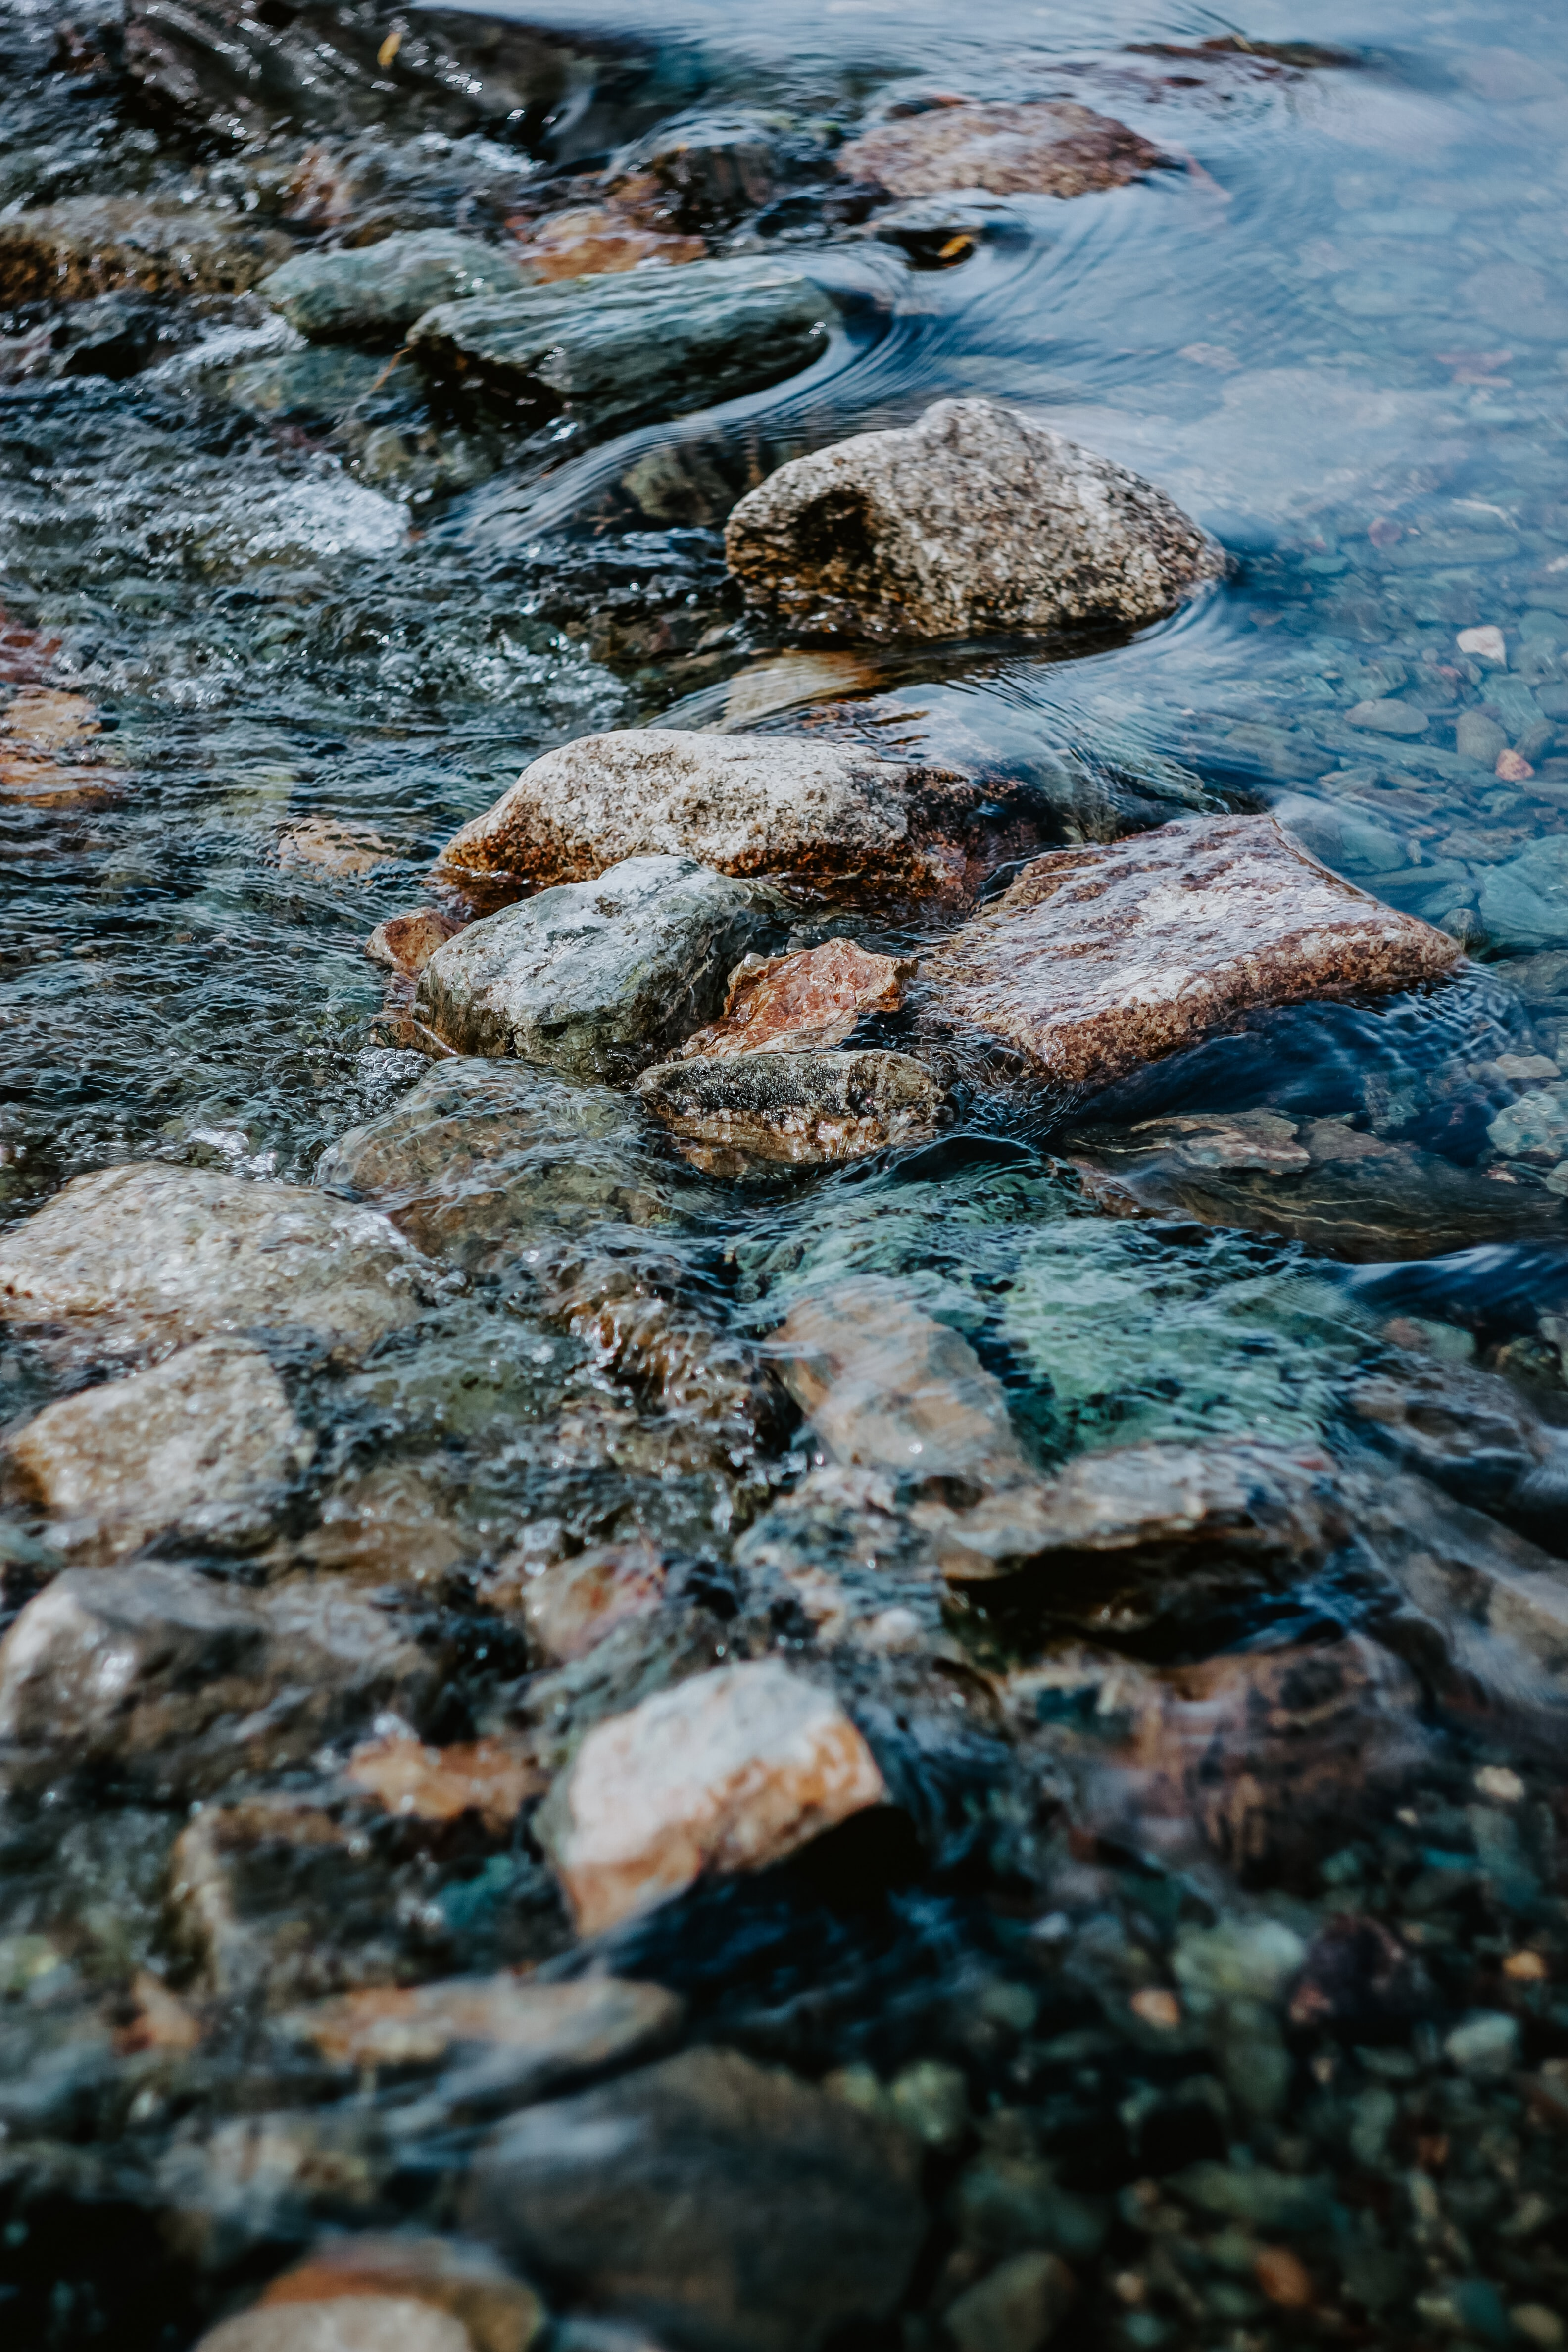
\includegraphics[height=5cm ]{laminar_turbulent_1.jpg}
% % 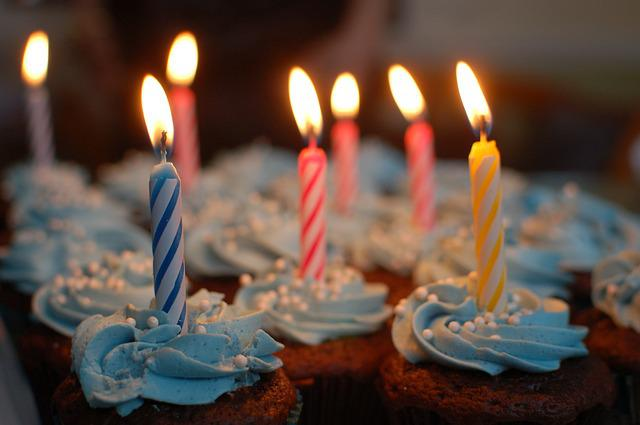
\includegraphics[width=5cm ]{llama_laminar.jpg}
% 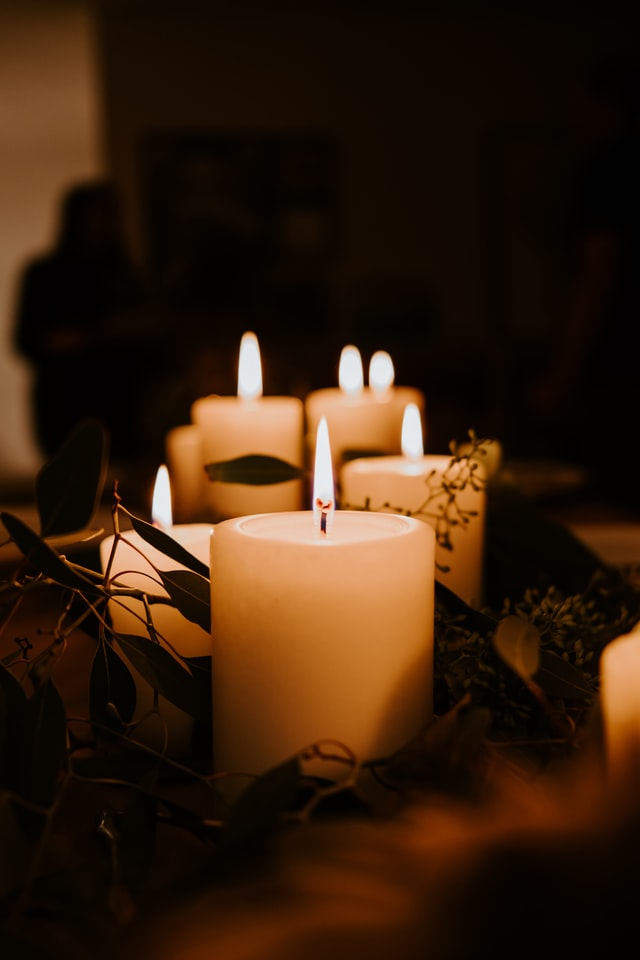
\includegraphics[height=5cm ]{velas.jpg}
% 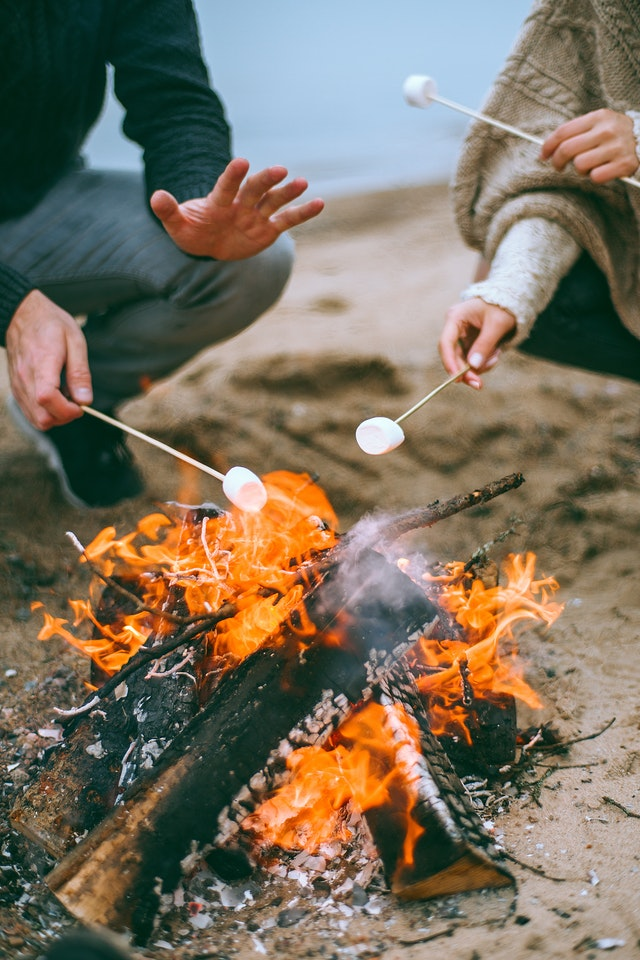
\includegraphics[height=5cm ]{llama_turb1.jpg}
% 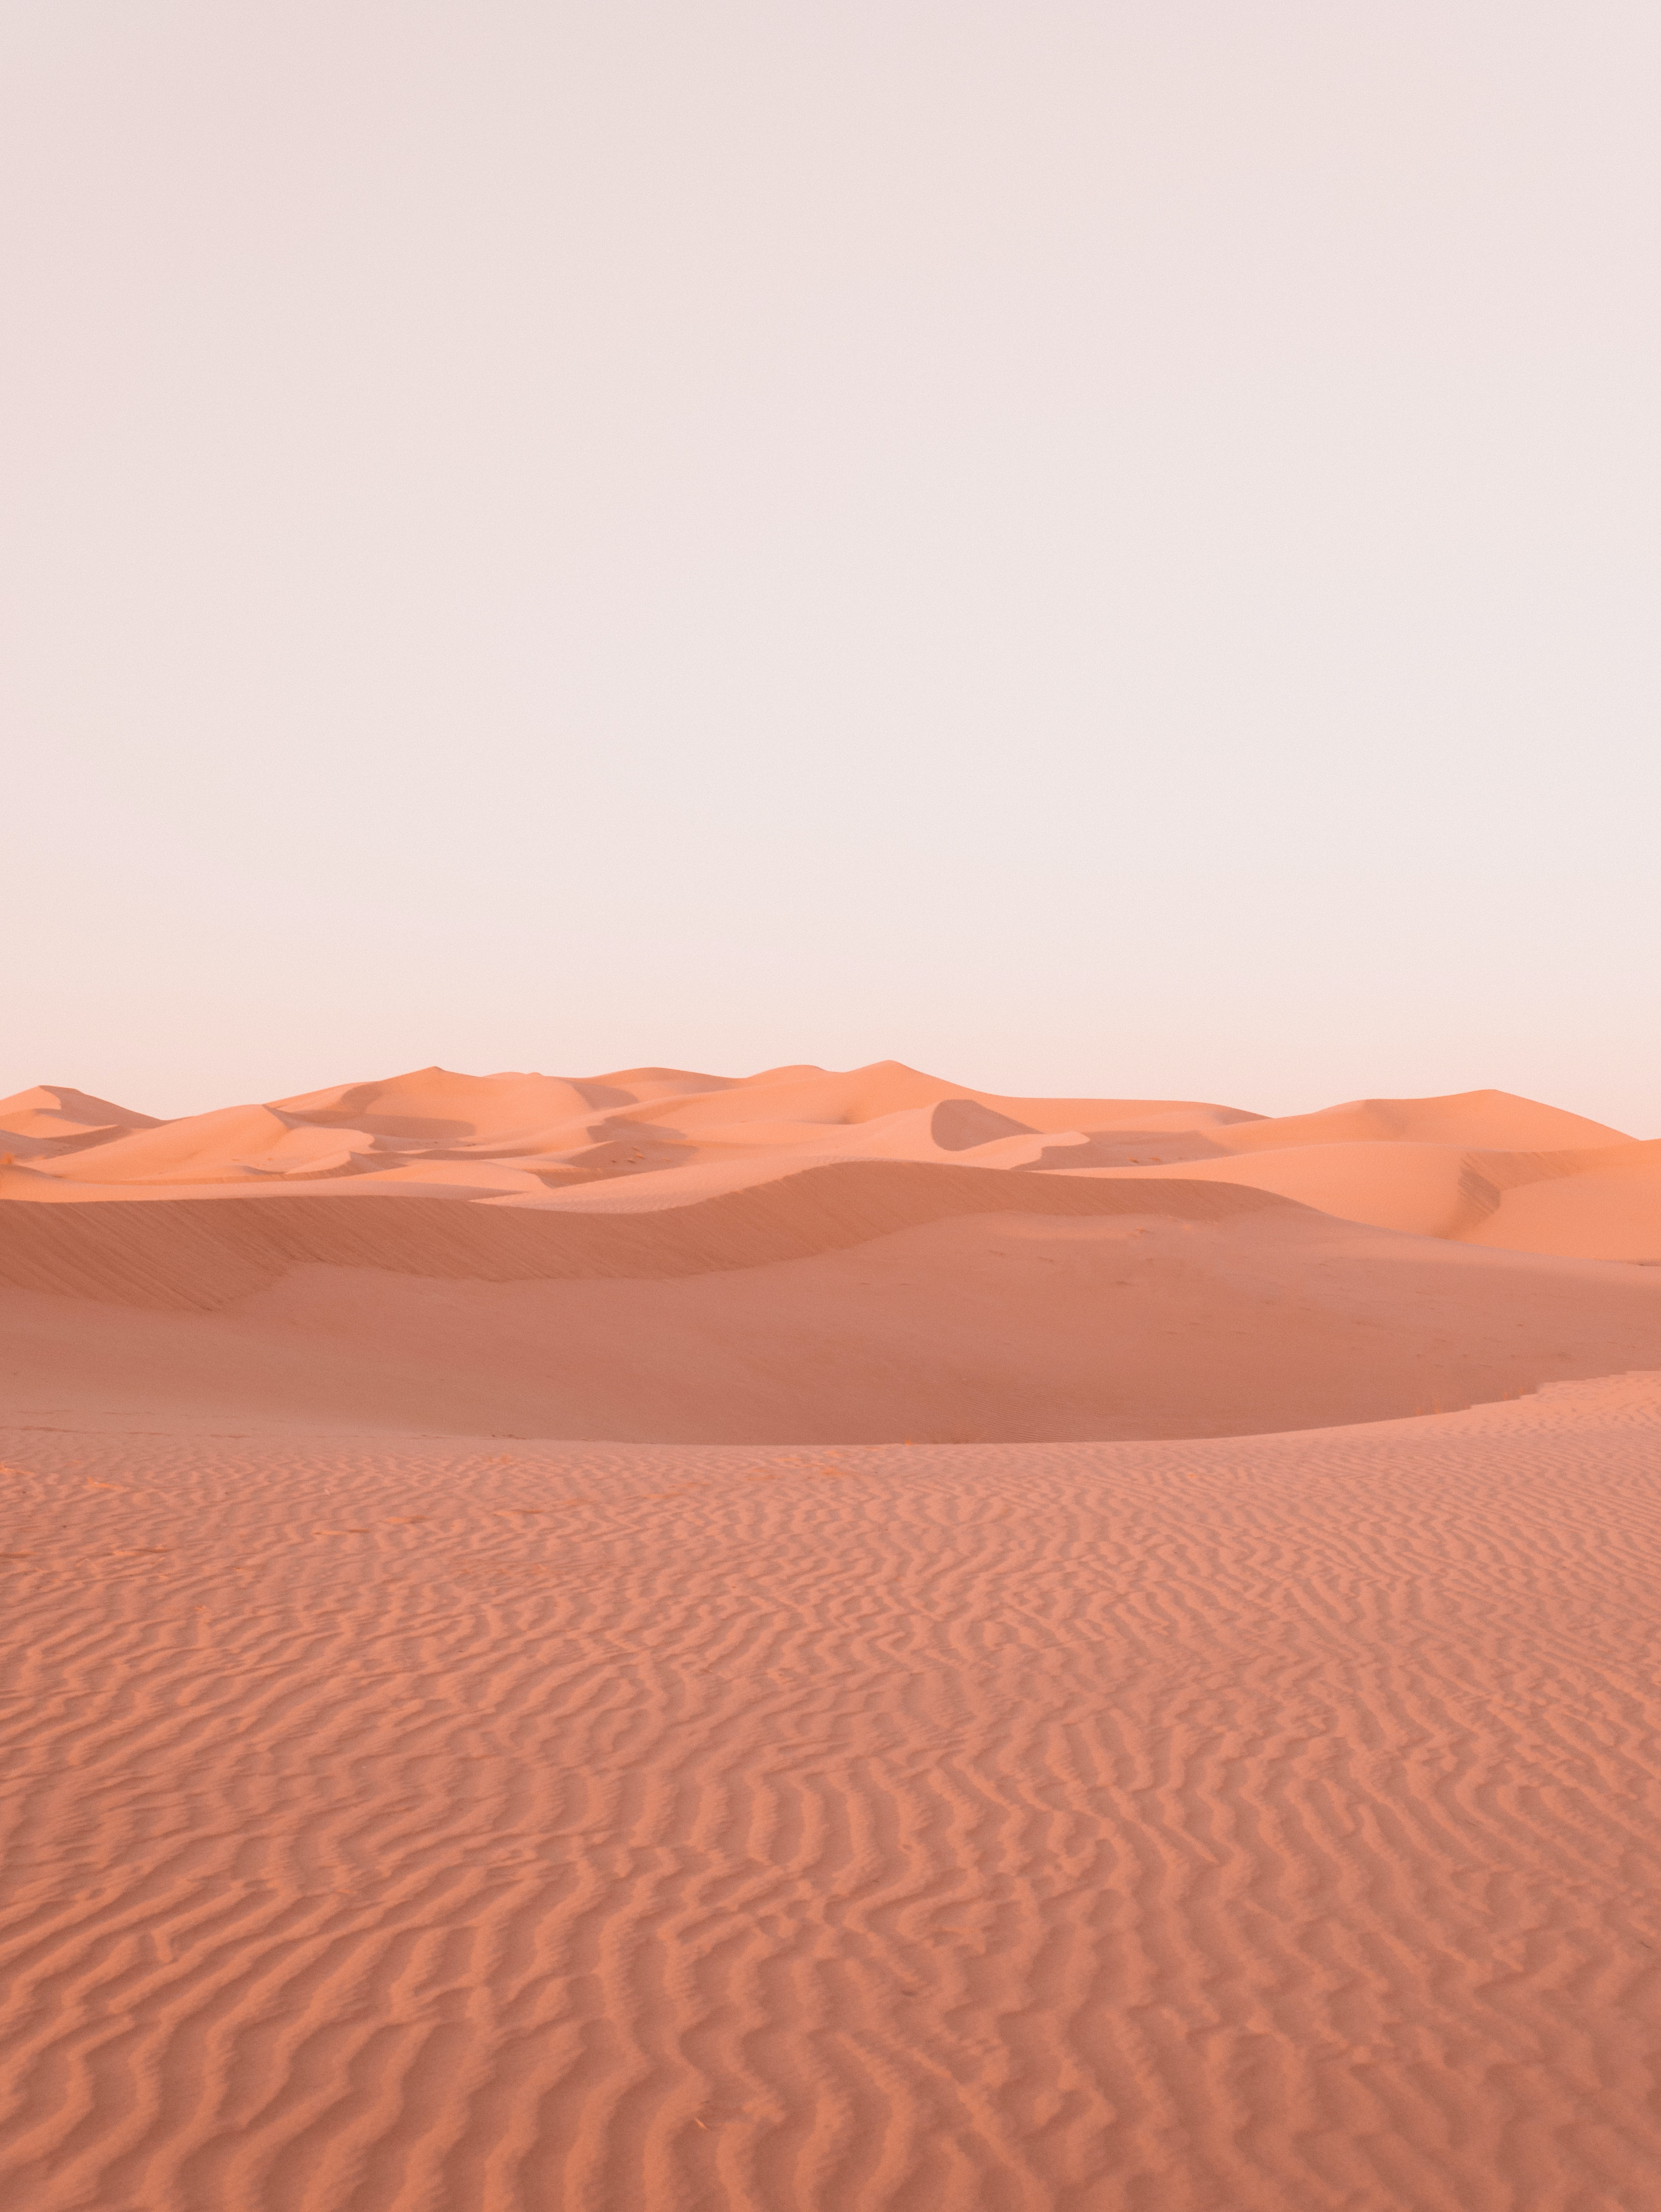
\includegraphics[height=5cm ]{imgs/streaks_dessert.jpg}
% 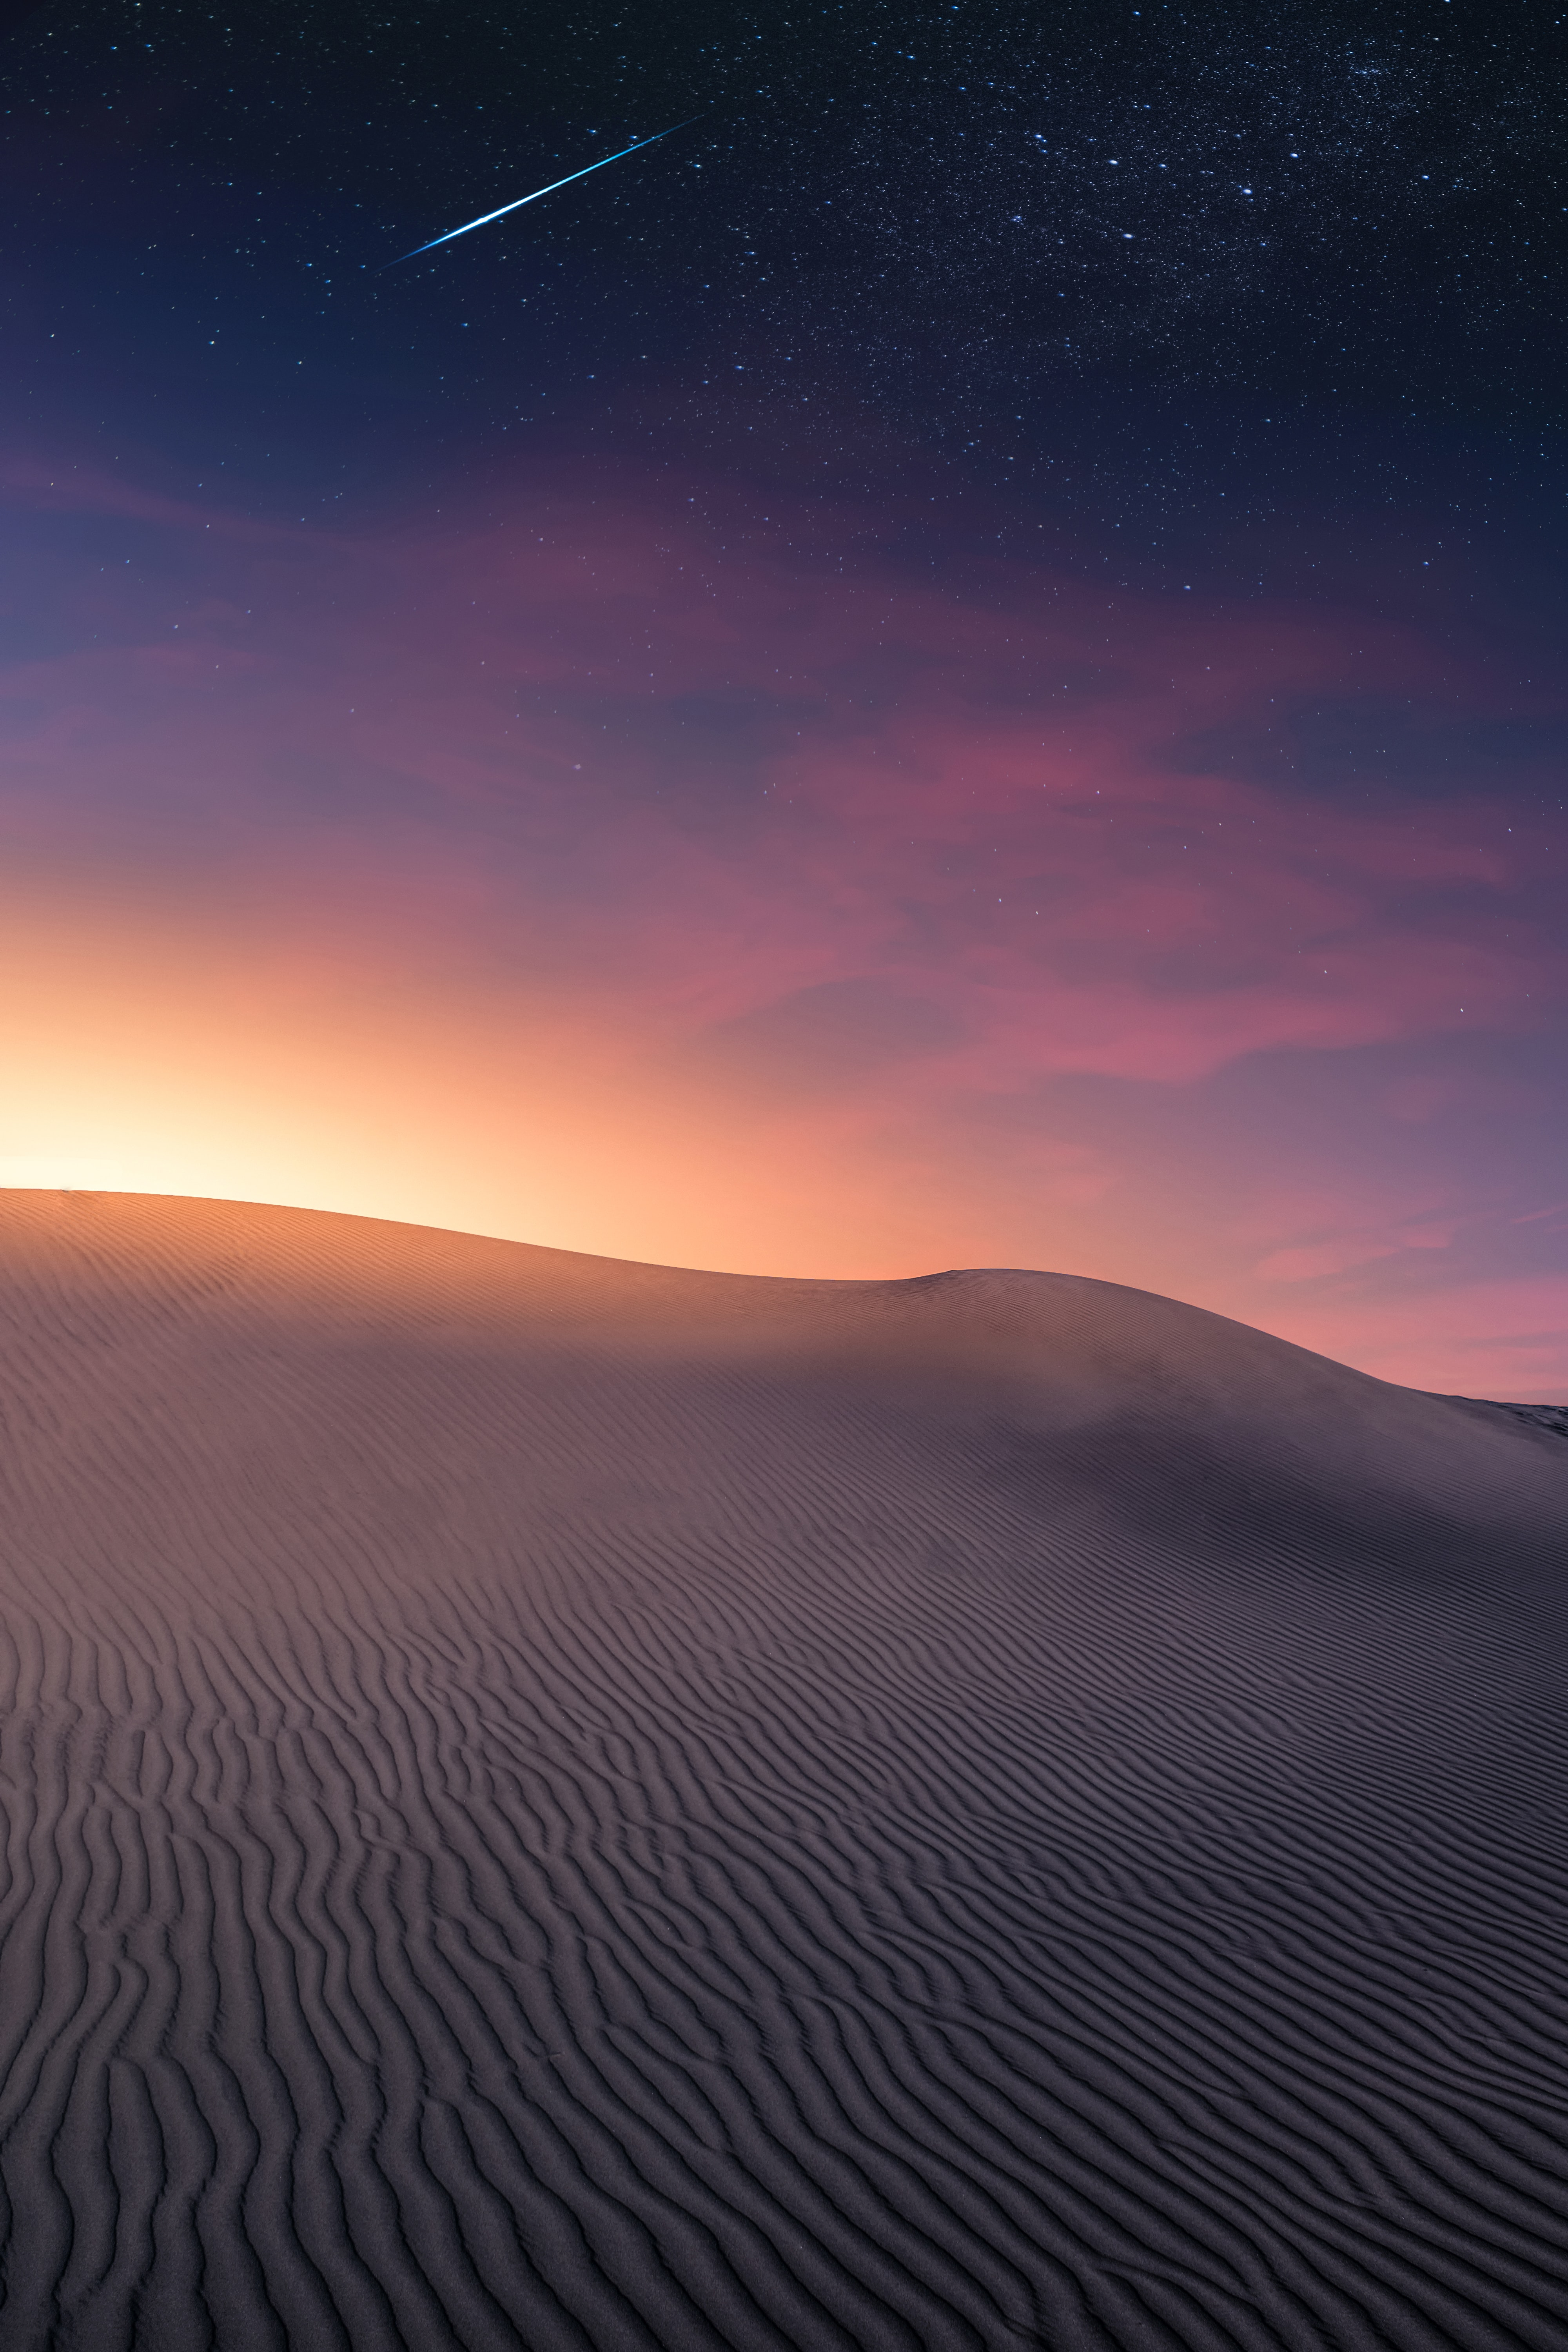
\includegraphics[height=5cm ]{imgs/streaks_dessert_2.jpg}

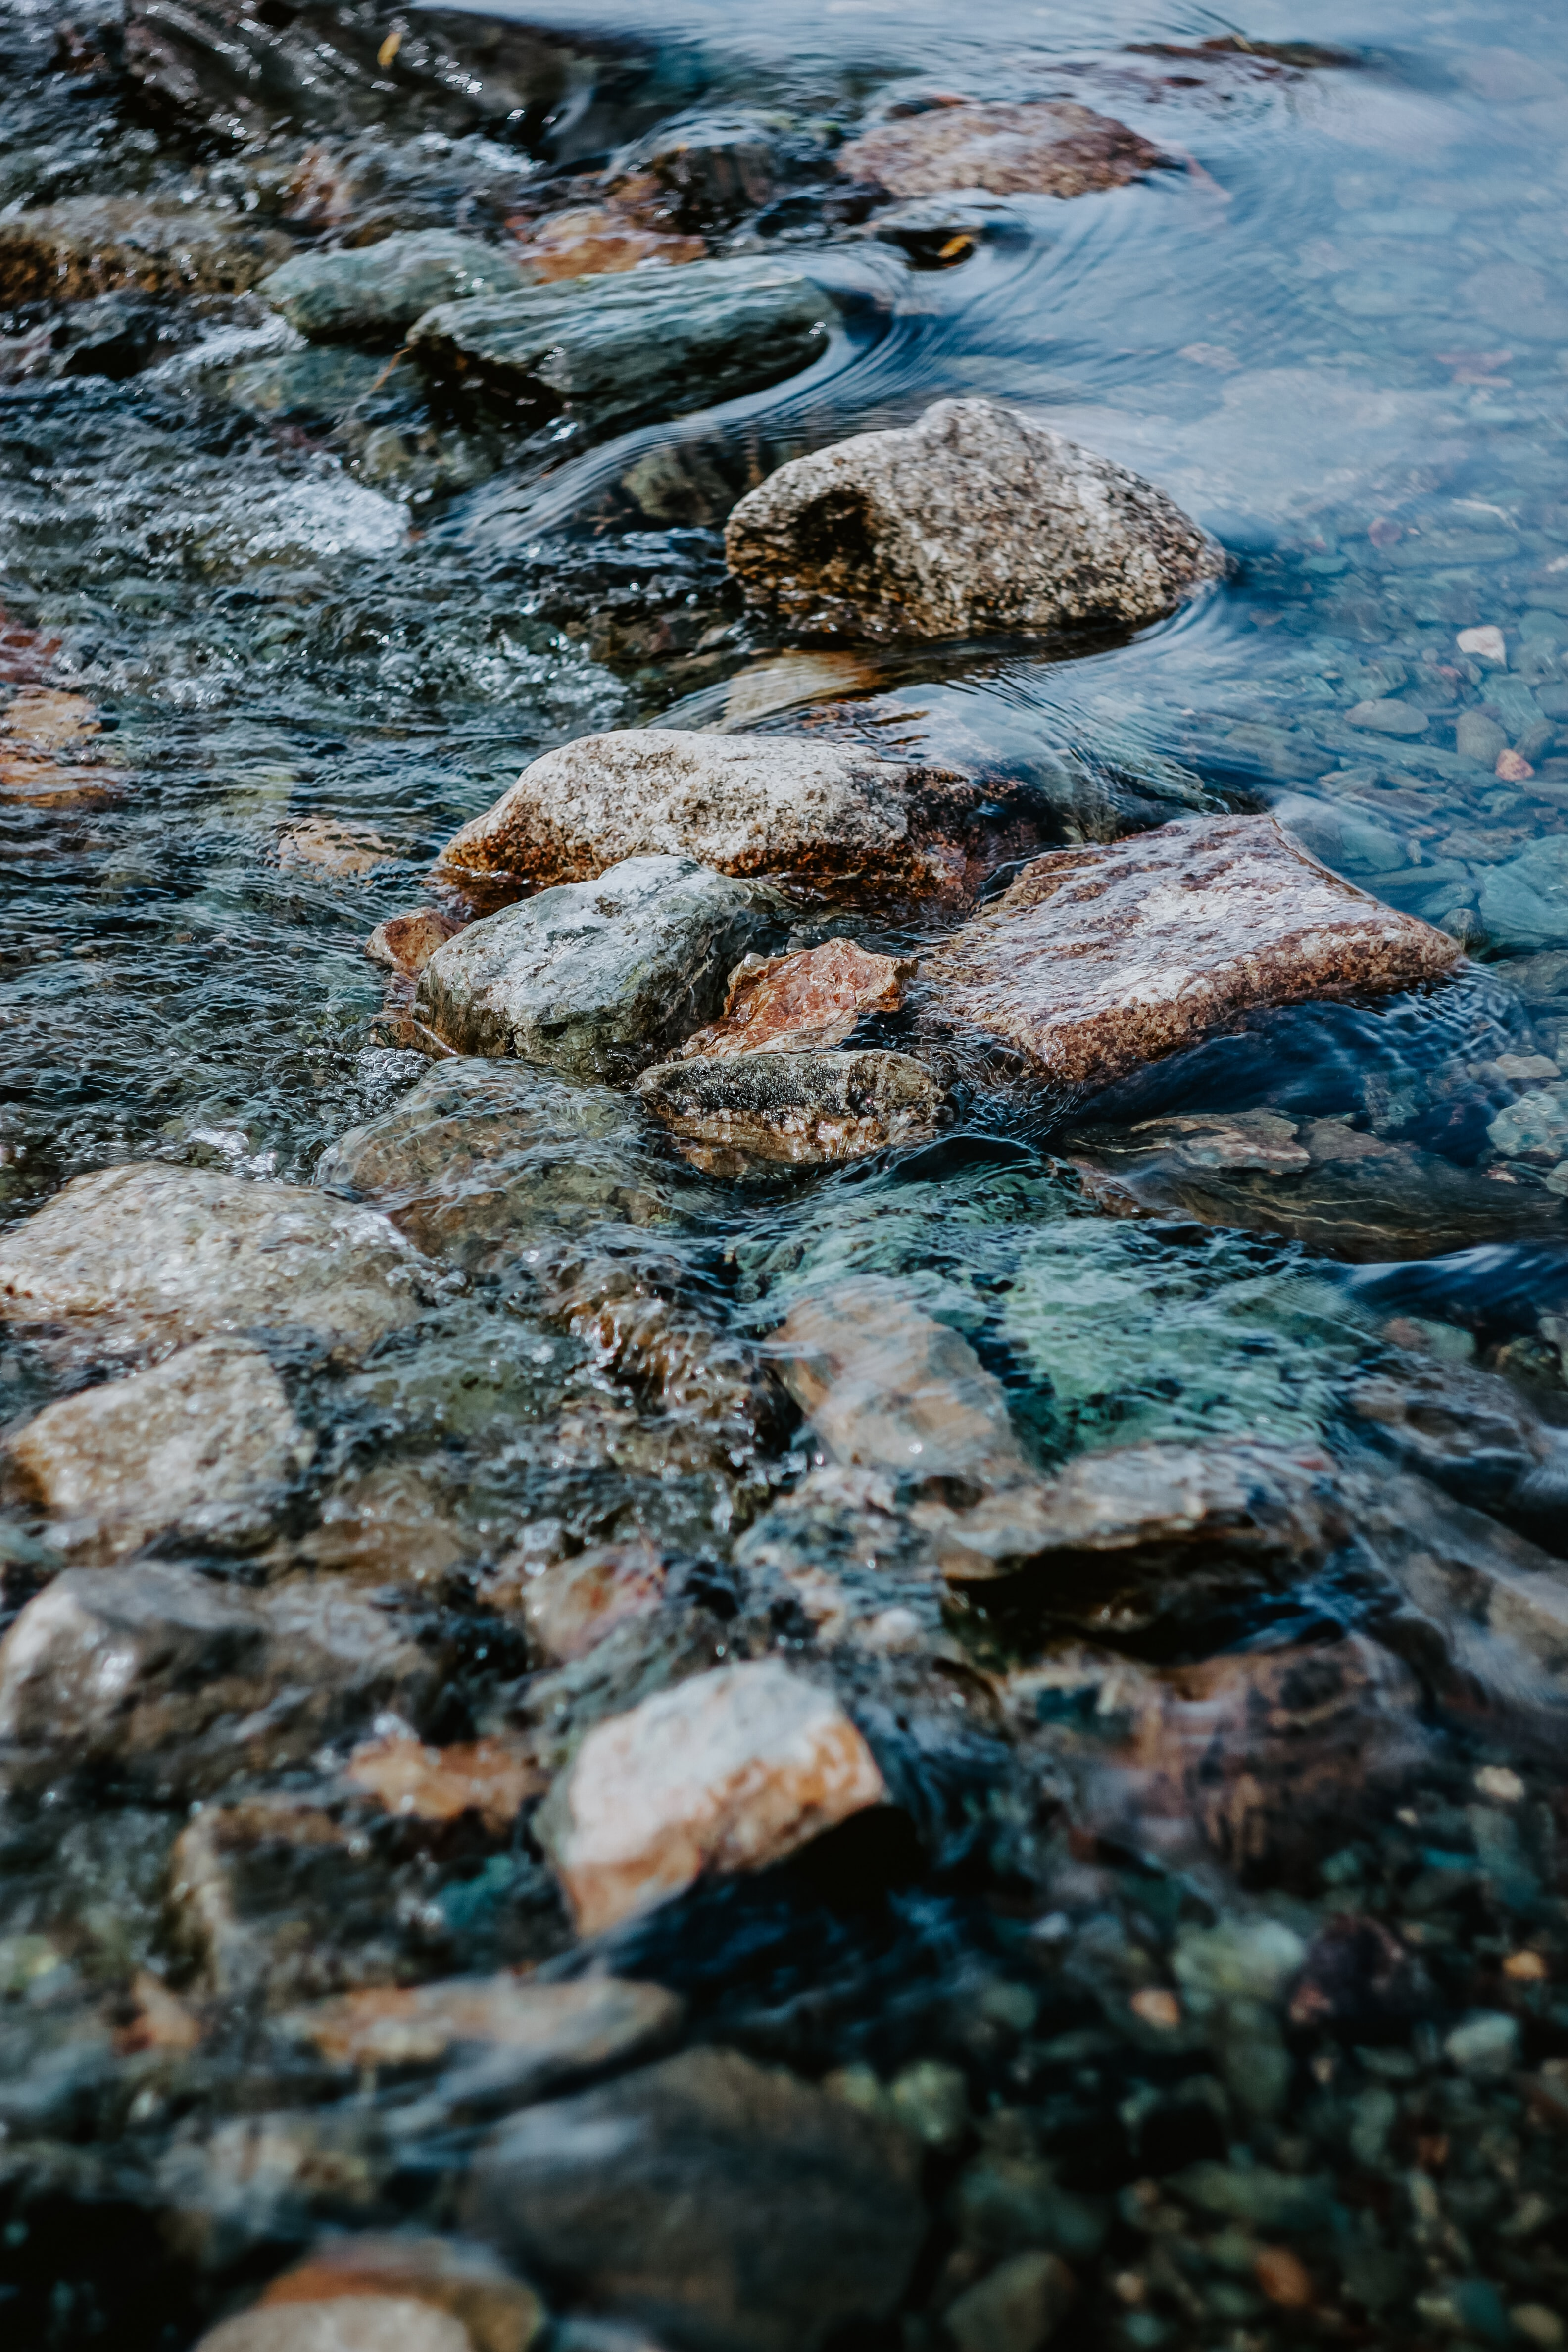
\includegraphics[width=0.24\textwidth ]{laminar_turbulent_1.jpg}
% 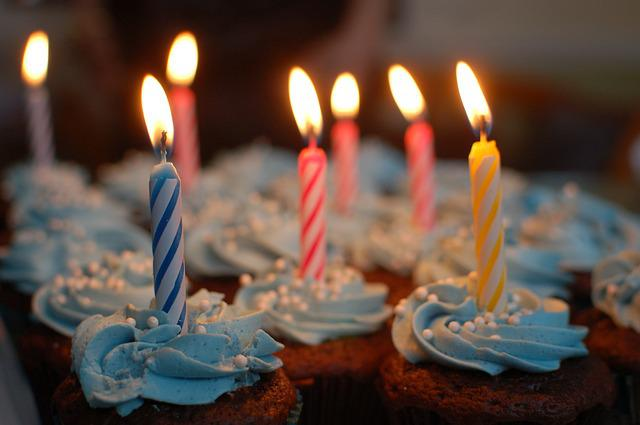
\includegraphics[width=5cm ]{llama_laminar.jpg}
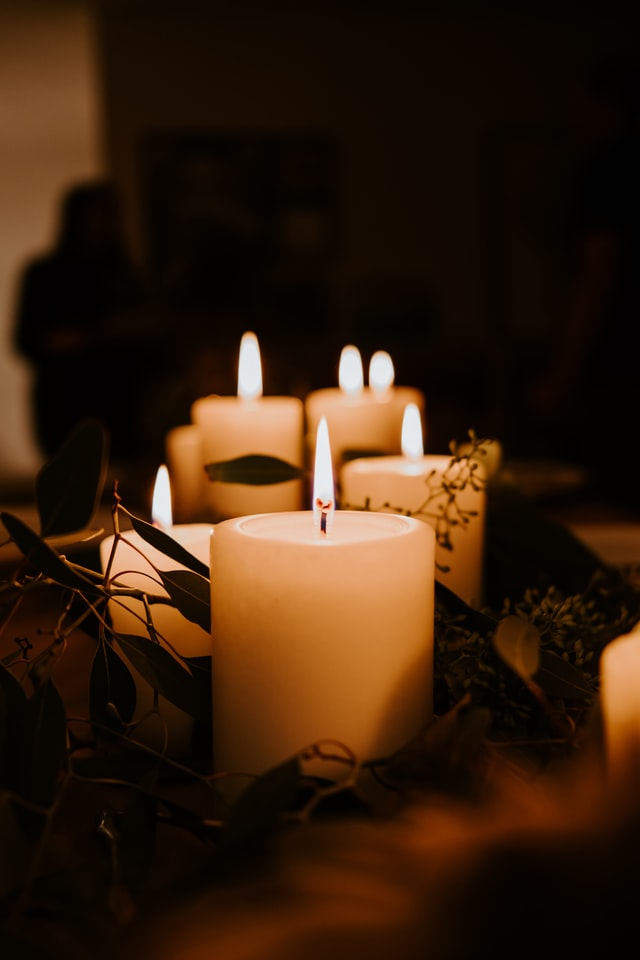
\includegraphics[width=0.24\textwidth ]{velas.jpg}
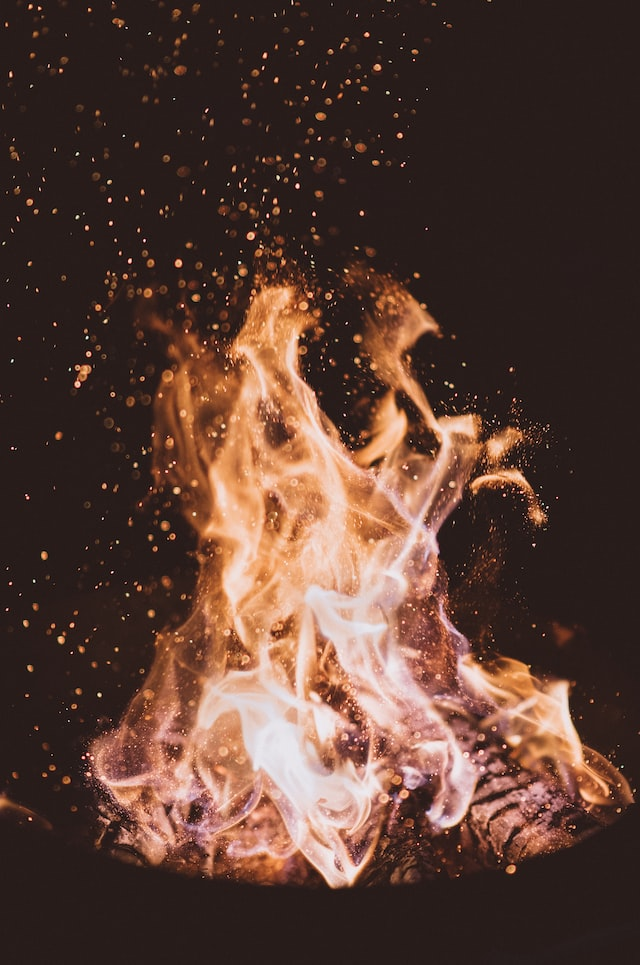
\includegraphics[width=0.24\textwidth ]{hoguera.jpg}
% 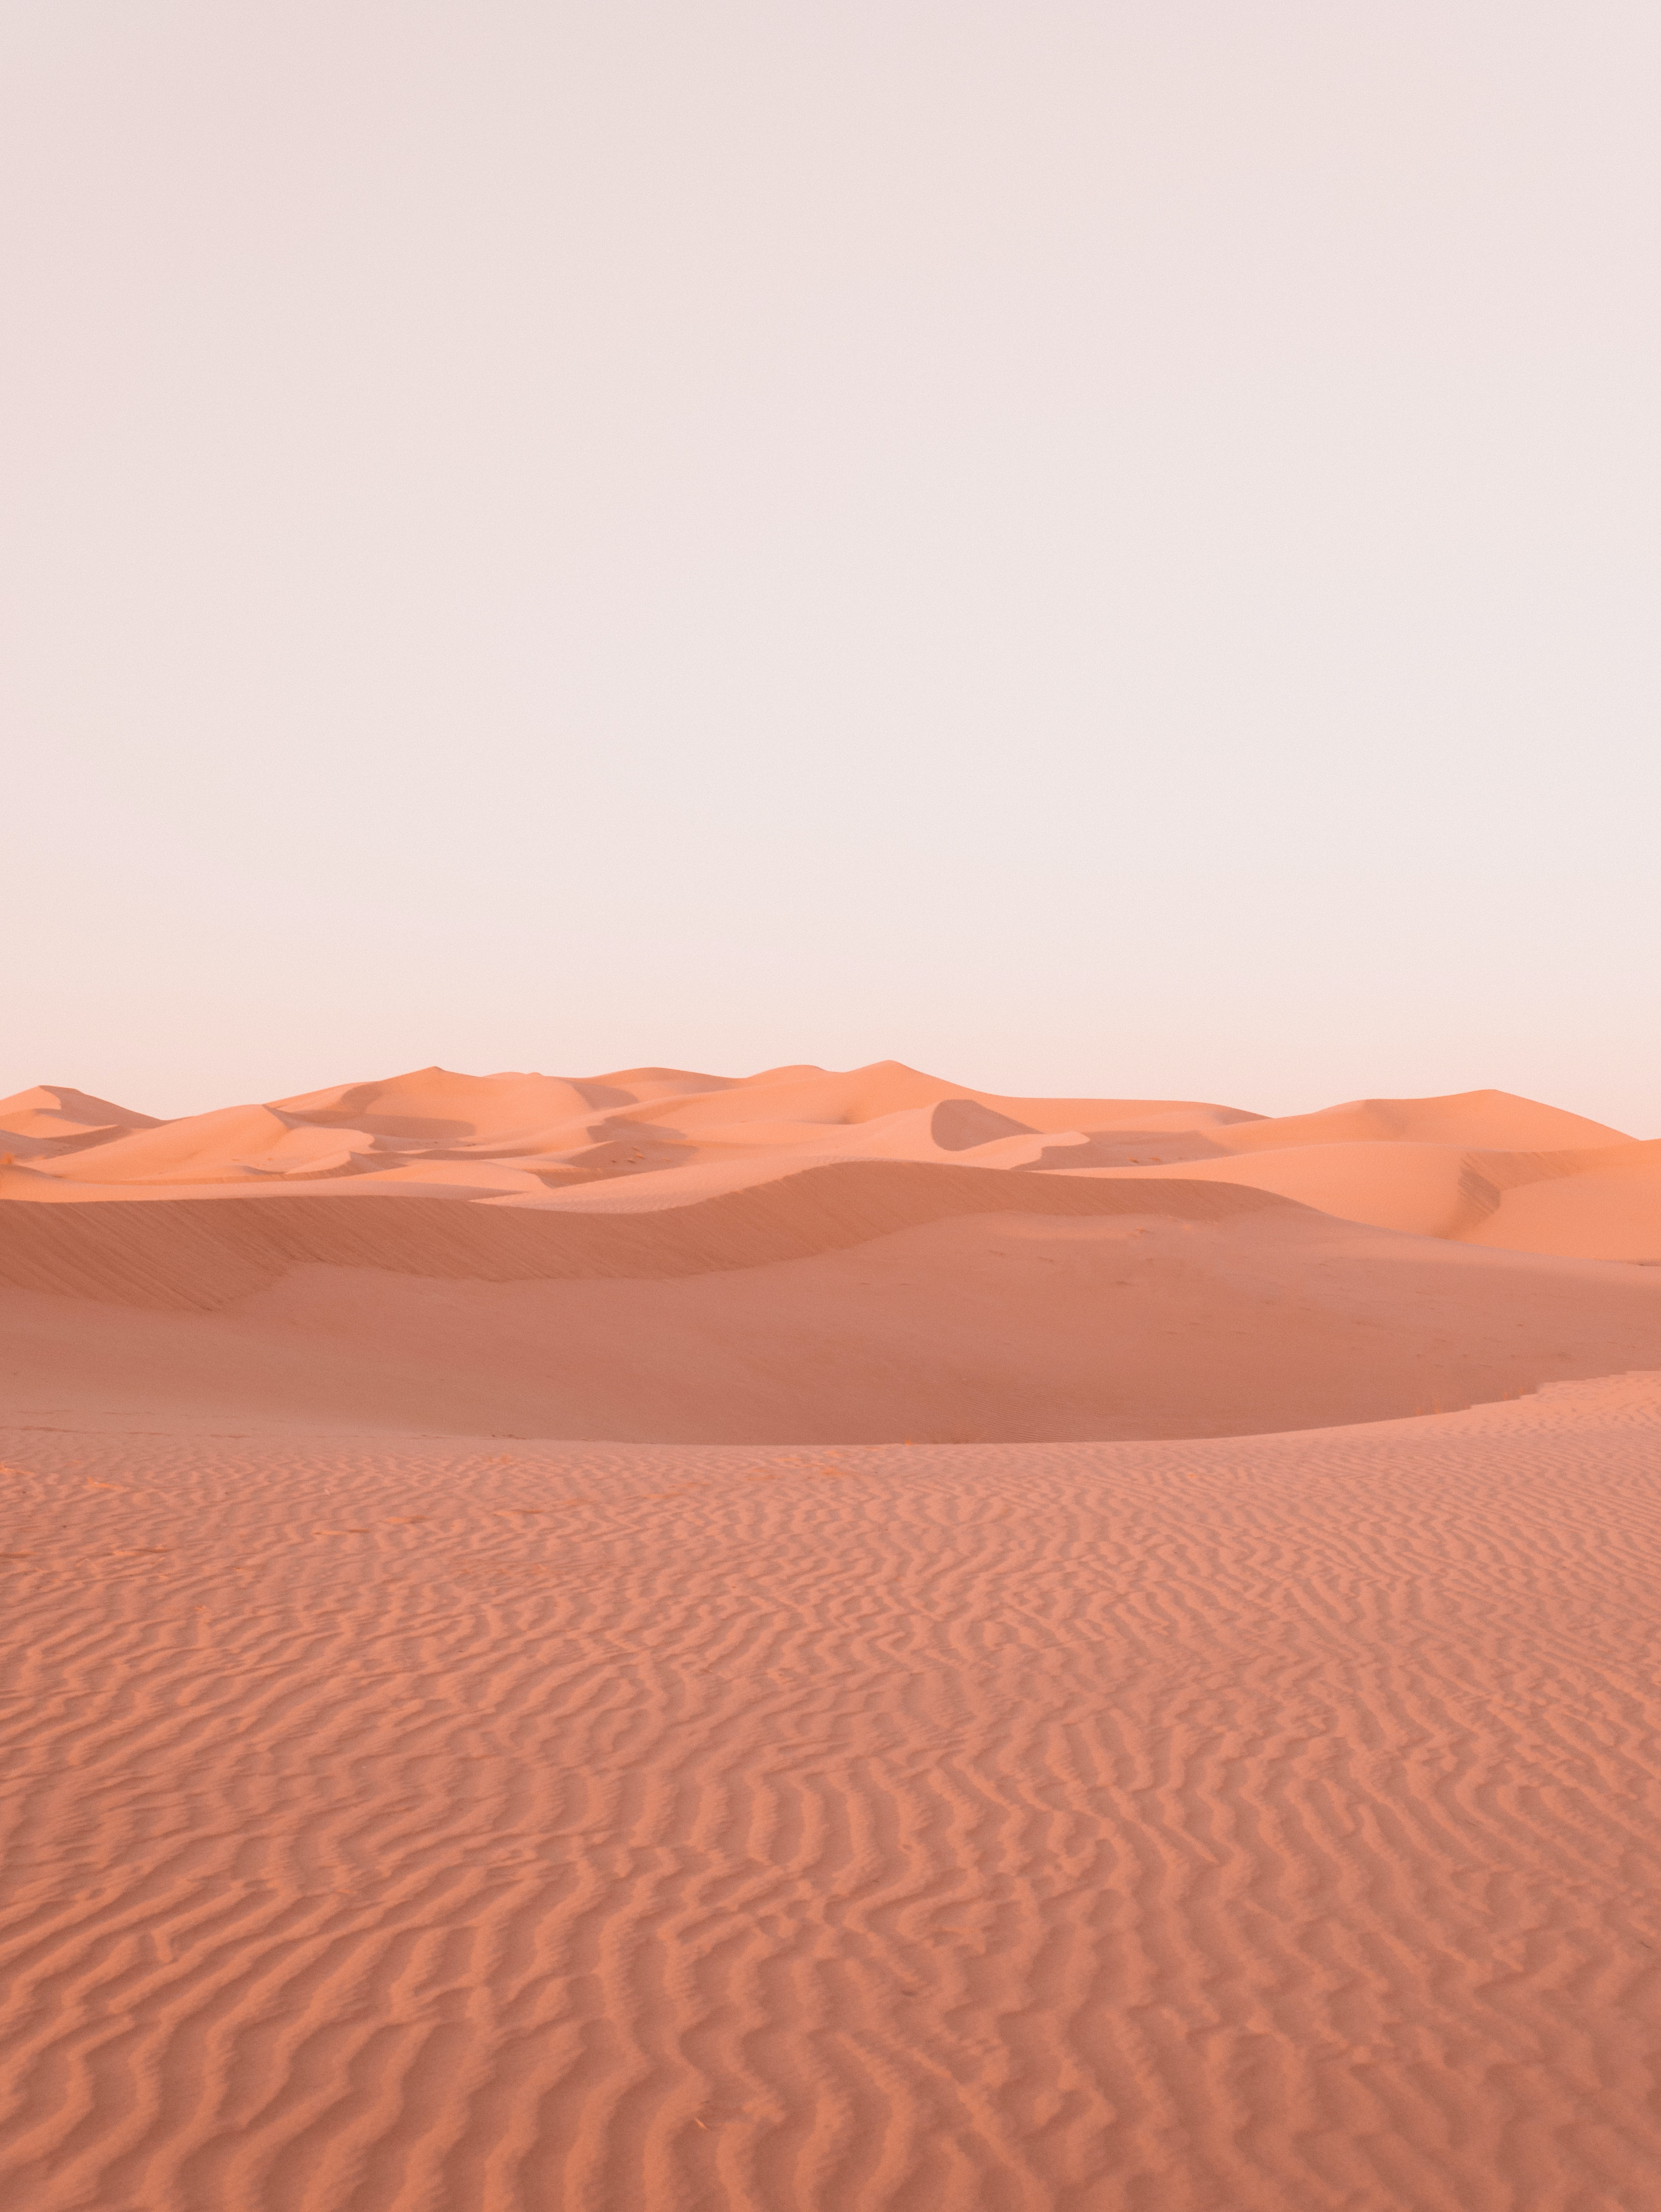
\includegraphics[width=0.2\textwidth ]{imgs/streaks_dessert.jpg}
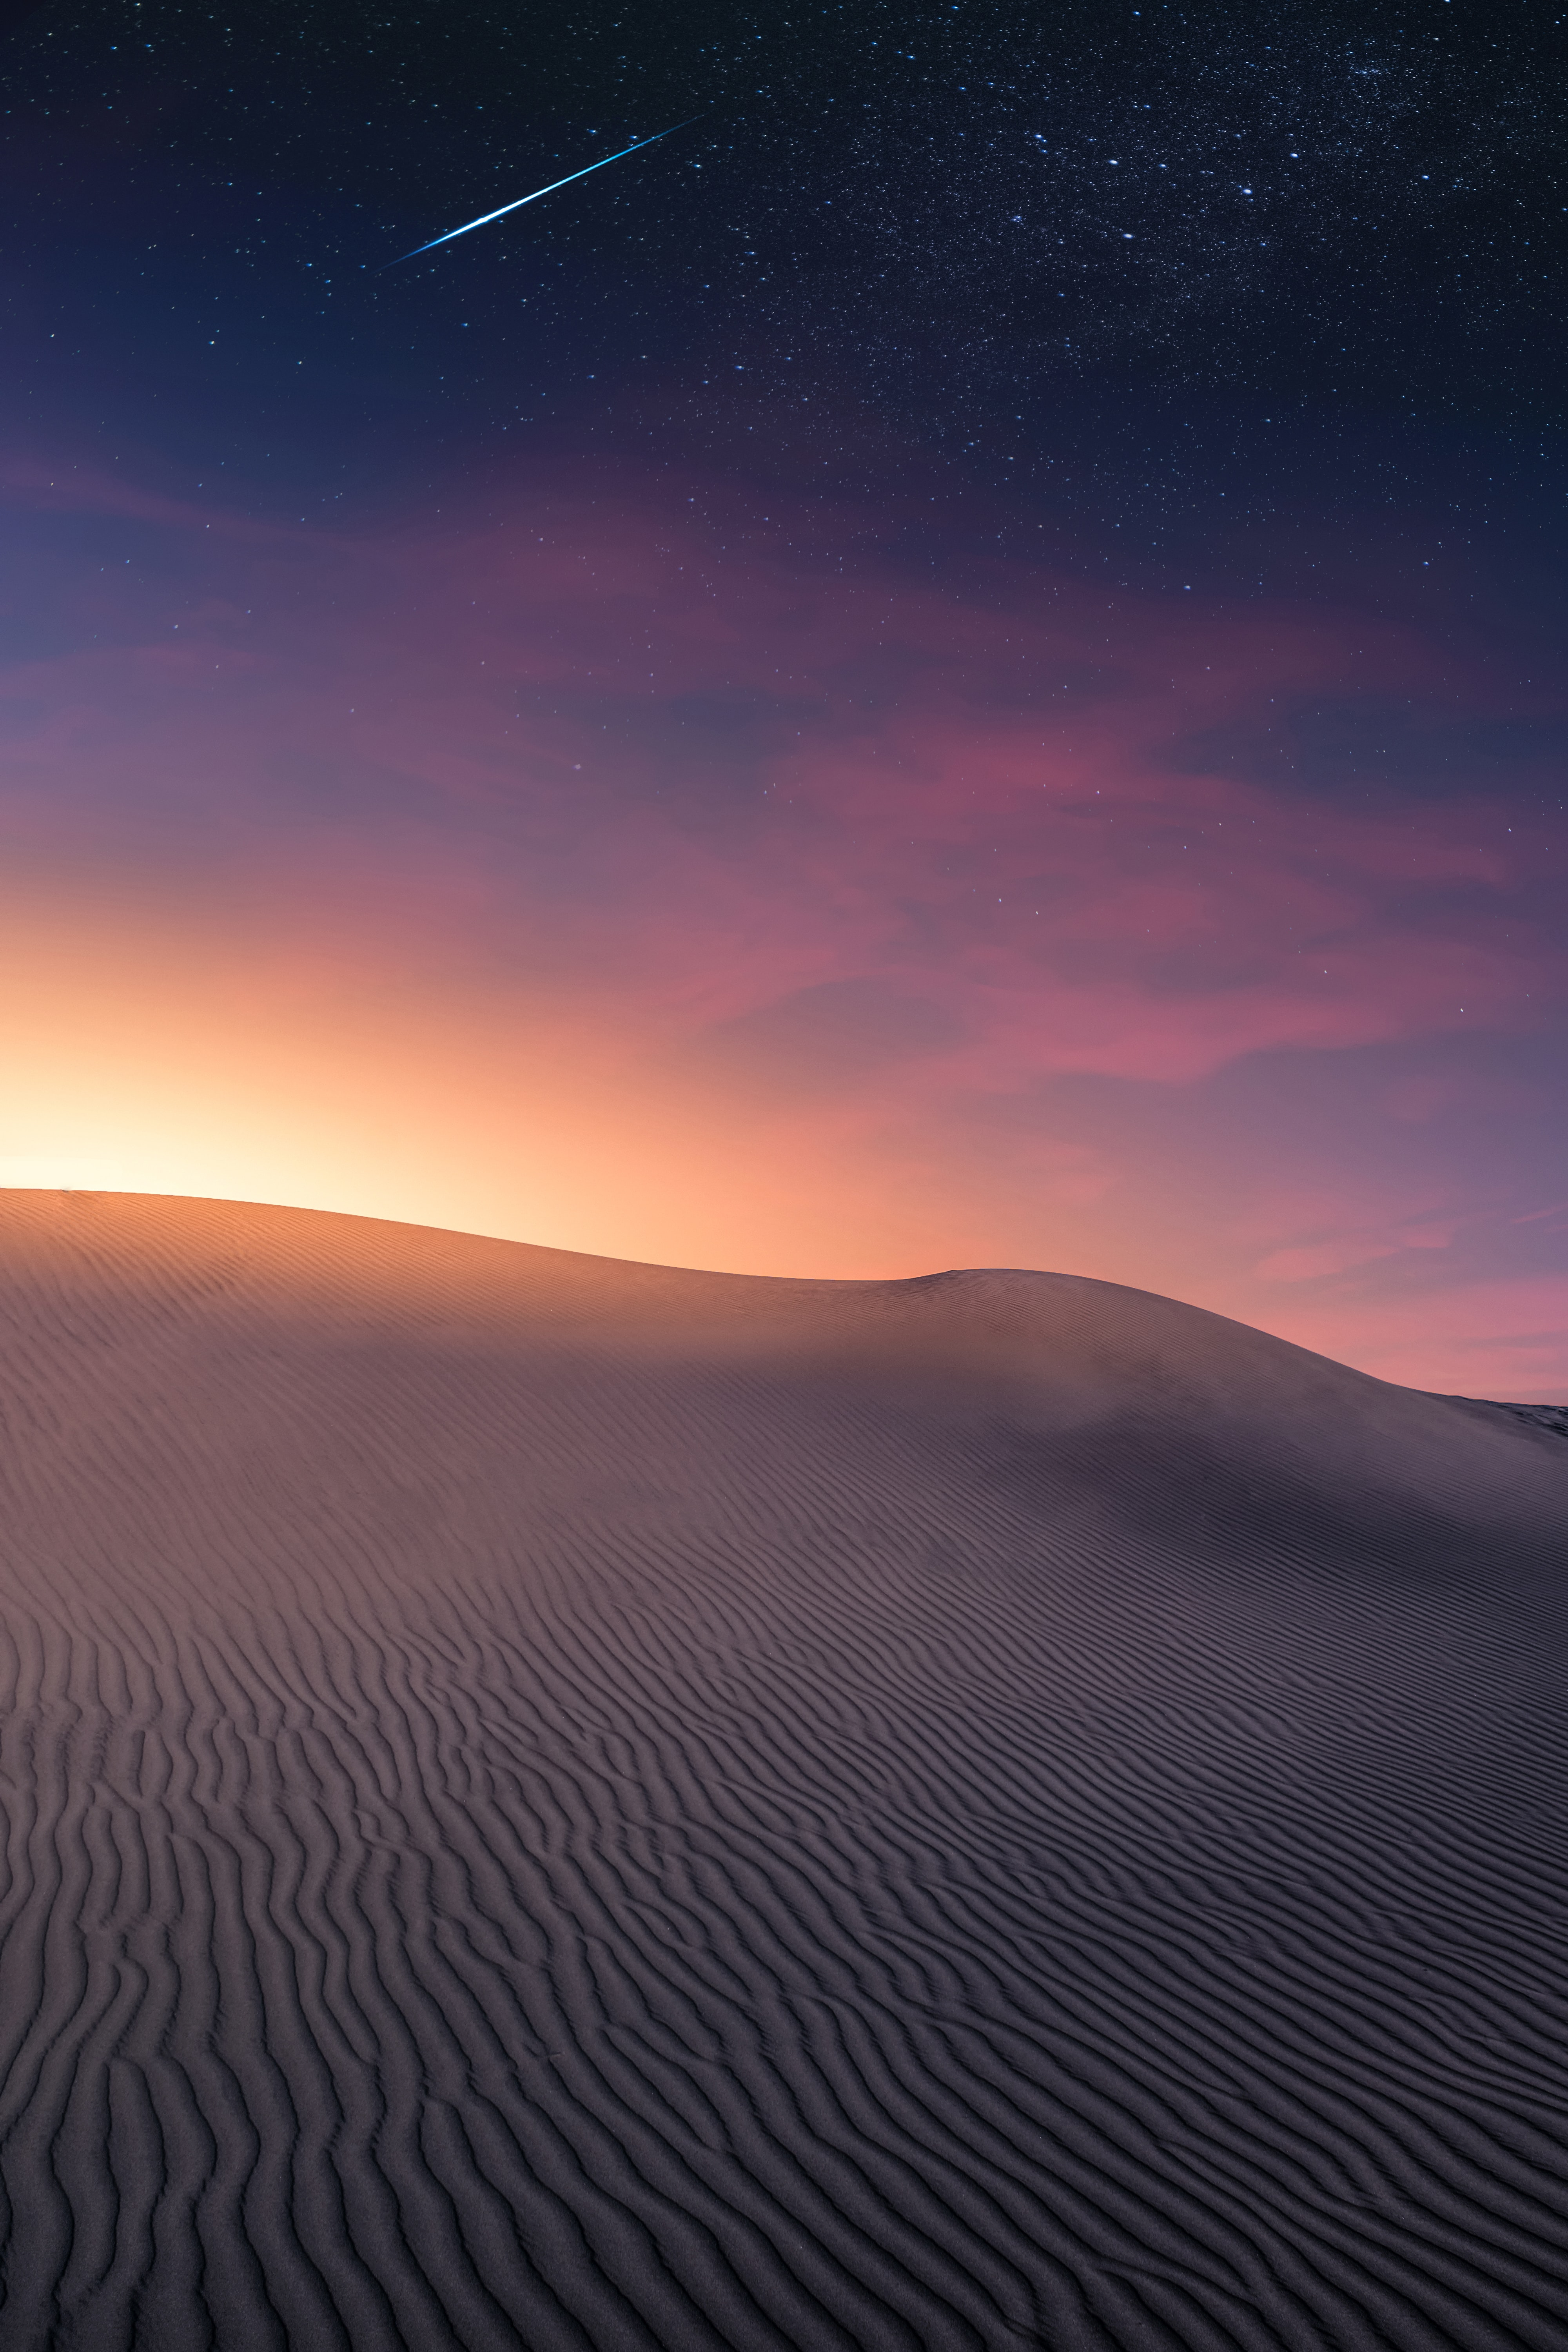
\includegraphics[width=0.24\textwidth ]{imgs/streaks_dessert_2.jpg}

\caption{ \label{fig:lam_turb} 
\highlight{
Examples of ordered laminar flow and chaotic turbulent motions in different materials. (Left) water in a shallow river, laminar on the righ side, turbulent after going through the rocks. (Mid-left) Fire in candles following an initial ordered upward motion (laminar). (Mid-right) Fire in a bonfire where the combustion gases are in a turbulent regime. (Right) Dunes in a desert flow due to the action of wind and gravity, the surface shows fine grooves as a result of the turbulent streaky structures of the wind flow over the sand surface. Figures extracted from: \url{https://unsplash.com/es/fotos/B8y6uvTnEvU} ,
\url{https://unsplash.com/es/fotos/e7cDMN6f0gs} ,
\url{https://unsplash.com/es/fotos/7qjqQjt7zXQ} and
\url{https://unsplash.com/es/fotos/MljwsnGwdOY} .   
}
}
\end{figure}

Laminar and turbulent regimes exhibit advantages and disadvantages depending on the application under consideration. 
In aerodynamic applications we usually focus in minimizing the friction present at the solid-wall boundary or maximizing the lift-to-drag ratio. coefficient. In that regard, the laminar boundary layer produces less friction than a turbulent boundary layer because 
\rev{it alters less the flow.}
\highlight{of its reduced momentum close to the wall.}
Detachment of the flow is an undesirable effect produced by strong adverse pressure gradients, and in this regard, the laminar-flow structure is more sensitive to detachment under APG conditions than a turbulent flow.

To study turbulent boundary layers (TBLs) and the effects of adverse pressure gradients (APGs) we will compare APG TBLs with a TBL subjected to zero-pressure-gradient (ZPG) conditions. A favourable pressure gradient (FPG) stabilizes and it can potentially relaminarize the boundary layer, and its effects are not critical such as those provoked by APGs, where the boundary layer can detach from the wall producing undesirable effects such as an increase in drag or even losing the aerodynamic control in airplanes.
In order to study this kind of wall-attached fluid-flow problem, first we should analyze the involved elements, such as the fluid and the solid elements.

\section{Fluid properties}

When studying the mechanics of a solid we track the positions, velocities and accelerations, forces and torques along its movement in space and time. This is the Lagrangian approach to Mechanics.
For a flow of particles or a fluid it is often more interesting to observe the flow variables at specific locations and observe the temporal change of those variables at those locations. This is the Eulerian approach that will be used to study the mechanics of a fluid flow. 

The main variables are the flow velocities, $\pmb{u}(\pmb{x},t)=u_i=(u,v,w)$, and the pressure $p(\pmb{x},t)$.
To simplify the study of adverse-pressure-gradient turbulent boundary layers the analyzed fluid is isotropic (its properties are the same in all directions) and Newtonian, which implies that the viscous forces are a linear function of the strain-rate tensor $s_{ij}=\pdv{u_i}/{x_j}$. As an example, the friction at the wall is $\tau_w=\mu \pdv{u}/{y}$,
where $\mu$ is a constant factor: the dynamic viscosity.
The density and viscosity of the fluid combines into the kinematic viscosity $\nu=\mu/\rho$ with units $[m^2/s]$. 
Note that we consider the density and viscosity as constant and not affected by changes in temperature.
\rev{, the temperature of the fluid is not relevant and the energy and momentum evolution are decoupled.}

\section{Solid properties}
In general, the solid boundaries are curved, specially in aerodynamic applications where the curvature is used to create differences in pressure that lead to forces in the desired directions. The forces in the direction of the inflow are called drag and the forces in the perpendicular direction is called lift. For curved boundaries, different coordinate systems are used. The local system of coordinates that changes with the solid boundary is where the surface forces are calculated. The surface forces are then projected onto the global coordinates associated with the inflow to obtain the lift and drag.
For flat plates with zero angle of attack the global and local coordinates are the same.
The surface of the flat plate that we study is rigid and smooth, and no exchange of heat or mass is produced between the fluid and the solid. In the interface fluid/solid the only interaction is due to pressure and viscous forces that adapt the fluid velocity to the solid surface velocity.
The flat plate will be considered to be static in the global system of coordinates.


\section{Boundary layers}

Boundary layers are regions inside a fluid flow where certain features or changes in the properties of the fluid are concentrated. Historically the first idea of boundary layer is set for the adaptation region of the fluid momentum from outer conditions to the conditions in a solid surface.
Other boundary layers are for example thermal boundary layers where the focus is on the change of thermal properties.

When we consider the flow around a solid object in incompressible conditions, the flow can detect the presence of the solid object and adapt its trajectory. The flow then surrounds the solid starting from the leading edge and close to the solid surface the boundary layer is the region where the velocity of the flow adapts from the solid surface velocity to the outer-flow velocity. The boundary-layer thickness has to be defined according to the main idea of a region of the fluid close to the solid wall that encloses the major viscous effects created due to the fluid/surface interaction. An obvious effect of the presence of a wall is that the streamwise velocity has to adapt from the velocity of the solid boundary to the exterior velocity, commonly called velocity at the infinity or freestream velocity $U_{\infty}$. 
In general, for a certain streamwise location, the velocity is measured in the wall-normal direction, obtaining a profile of instantaneous streamwise velocity $u(y,t)$. Then $U_{\infty}=U(y\rightarrow \infty)$ (where capital letter denotes mean velocity) is the unperturbed velocity and can change from one streamwise position to another.
In the case of zero-pressure gradient boundary layers, $U_{\infty}$ is taken as constant, since in a steady flow in the absence of viscous forces, $\pdv{U}/{x}$ should be zero. 

Since an obvious property of the boundary layer is the adaptation of the streamwise velocity, the boundary layer can be defined using this property and the $99\%$ thickness $\delta_{99}$ is defined as the wall-normal position where $U(y=\delta_{99})~=~0.99U_{\infty}$.
In Fig.~\ref{fig:lam_turb_profiles} we show an example of how the mean streamwise velocity $U(y)$ adapts from the velocity at the wall $U(y=0)=0$, to the outer velocity $U_{\infty}$ on laminar and ZPG TBL profiles.

\begin{figure}[h!]
\centering
% \captionsetup{width=0.99 \textwidth}
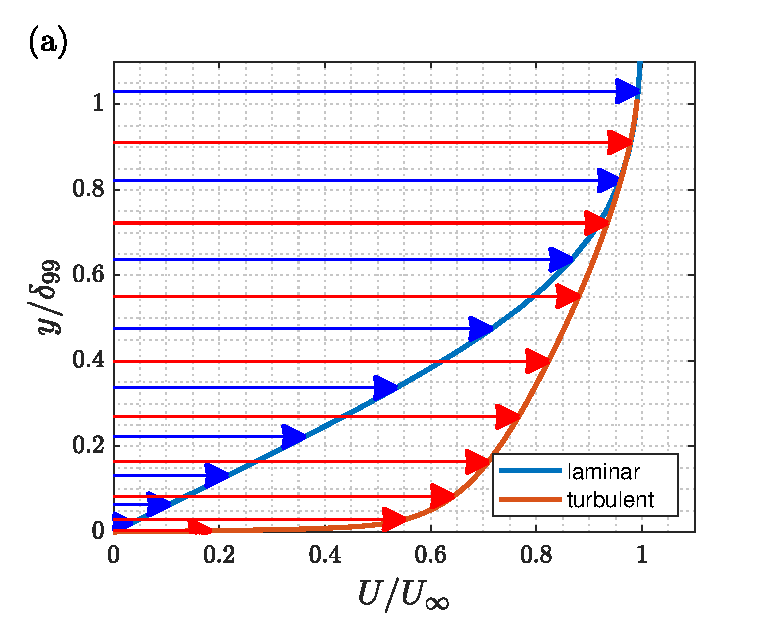
\includegraphics[width=0.6\textwidth]{imgs/lam_turb/ZPG_lam_turb.eps}
\caption{ \label{fig:lam_turb_profiles} Mean streamwise velocity profile of a laminar and a turbulent boundary layer subjected to a ZPG.
   }
\end{figure}

In the case of curved boundaries, the curvature induces a pressure gradient since the incoming flow has to adapt to the curvature of the wall. On a flat plate, a pressure gradient can be produced by controlling the exterior flow, usually the streamwise gradient of the streamwise velocity $\pdv{U_{\infty}}/{x}$


\subsection{Turbulent boundary layers}
The characteristics of a boundary layer change radically depending on the laminar/turbulent regime.
In a laminar boundary layer, any perturbation produces shear stresses and therefore, viscous forces, which are transported by the momentum of the flow and eventually dissipated by the viscous dissipation. 
Highly-energetic perturbations, flow configurations or certain viscosity/momentum forces ratios are unstable, implying a change of regime, usually from the laminar regime to turbulence. 
The ratio between inertial and viscous forces is called Reynolds number $\Rey=U_{sc} L_{sc} / \nu$, and depending on the chosen velocity and length scales $U_{sc}$ and $L_{sc}$ we would be analyzing different phenomena. The Reynolds number where a flow configuration changes regime is called critical Reynolds number $\Rey_c$.
Note that if $U_{sc}=U_{\infty}$ and $L_{sc}=c$ where $c$ is the chord of a wing profile, then we are setting the global configuration of the problem. If we want to analyze a local phenomenon such as the different size of the flow scales close to the wall compared to the largest ones, we can use the Reynolds number based on the friction velocity $\Rey_{\tau}=u_{\tau}\delta_{99}/\nu$, where  $u_{\tau}=\sqrt{\tau_w / \rho}$.

In the turbulent regime, the momentum and energy of the flow initiate a cascading effect breaking the initial ordered motions into chaotic submotions. 
Eddies are generated, and they extract energy from the mean flow, then dividing into smaller eddies (note that there is also an inverse cascade of energy transfer from smaller to larger scales). Then a transport of energy between large and small eddies is produced. Eddies are regions with strong shear stresses, therefore the viscous forces are stronger and produce a dissipation of the kinetic energy.
The boundary layers studied here are momentum boundary layers that confine the turbulent perturbations and mayor viscous effects produced because of the presence of a solid boundary.

\rev{In a turbulent boundary layer, the thickness of the boundary layer should delimit the region of the flow close to the wall that exhibit the turbulent fluctuations and viscous forces produced by the presence of a solid boundary,} leading to different definitions for the boundary-layer thickness.
For laminar BLs and ZPG TBLs, the previously-defined $\delta_{99}$ thickness, where the mean velocity of the flow is $99\%$ of the exterior velocity, is valid and is based only on the adaptation of the mean streamwise velocity to that of the outer flow.
For other TBLs with pressure gradients, the outer velocity can have gradients in the streamwise and wall-normal directions. In the case of TBLs subjected to streamwise pressure gradients we can use an approach based on the level of turbulence such as the one used in \cite{diagnostic_Vinuesa} where the boundary-layer thickness is such that it captures the turbulence up to certain turbulent level.
This approach is useful for the dataset that we use, since the turbulent levels outside the TBL are minimal, both in the simulations \citep{EAmorZPG, bobke2017, Pozuelo_JFM_22}, and in the experimental databases \citep{Sanmiguel_PRF}.
If the freestream turbulent level is high, the method in \cite{diagnostic_Vinuesa} is not applicable. 
Other methods have been proposed in the literature and a review was given by \cite{d99_determination_2020}.

Turbulence exhibits a wide range of motions, and one way to study and characterize turbulence is through decomposition of those characteristics. 
The first approach is an statistical characterization where we can divide the flow variables into a mean or average value and a perturbation; this is known as the Reynolds decomposition \citep{Rey_decomp}.
The fluctuating character of the flow is shown for a flat-plate TBL in Fig.~\ref{fig:lam_turb_development} where we show contour levels in snapshots of the instantaneous streamwise velocity. \highlight{In Fig.~\ref{fig:lam_turb_development}(a) we show the initial laminar ZPG flow-field used to initialize the APG simulation. The contours are smooth and show a well-defined laminar behaviour with small perturbations introduced to trigger turbulence. The red line is the position where $u=0.99U_{\infty}$. In Fig.~\ref{fig:lam_turb_development}(b) the turbulence is totally developed and correspond to the APG simulation when the final APG conditions are reached. The red line correspond to $U=U_e$ which is the outer velocity or ``edge velocity'' calculated through the method in \cite{diagnostic_Vinuesa}. It is possible to see how at different streamwise positions $x/\delta^*_0$ (where $\delta^*_0$ is the inflow displacement thickness) the instantaneous velocities close to the red line are decreasing, this is due to the APG boundary condition, where $U_e$ decrease along $x$ to produce a near-equilibrium APG. The edge velocity depends on the method used to determine the boundary-layer thickness.
}
\begin{figure}[h!]
\centering
% \captionsetup{width=0.99 \textwidth}
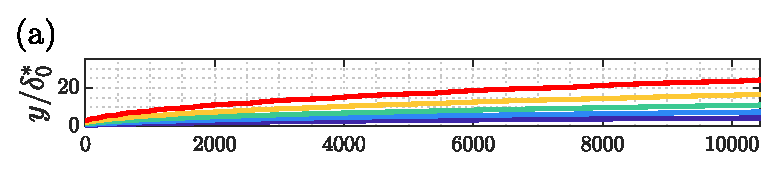
\includegraphics[width=0.99\textwidth ]{imgs/lam_turb/APG_laminar_test.eps}\\
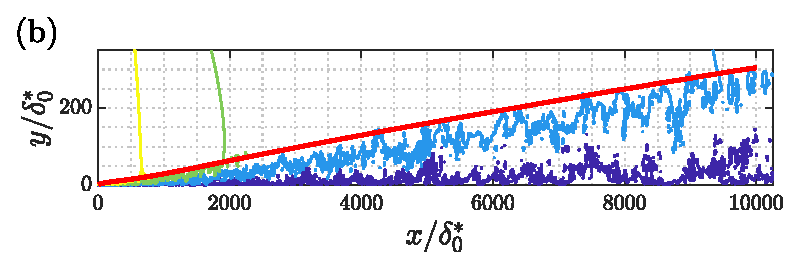
\includegraphics[width=0.99\textwidth ]{imgs/lam_turb/APG_turb_test.eps}
% 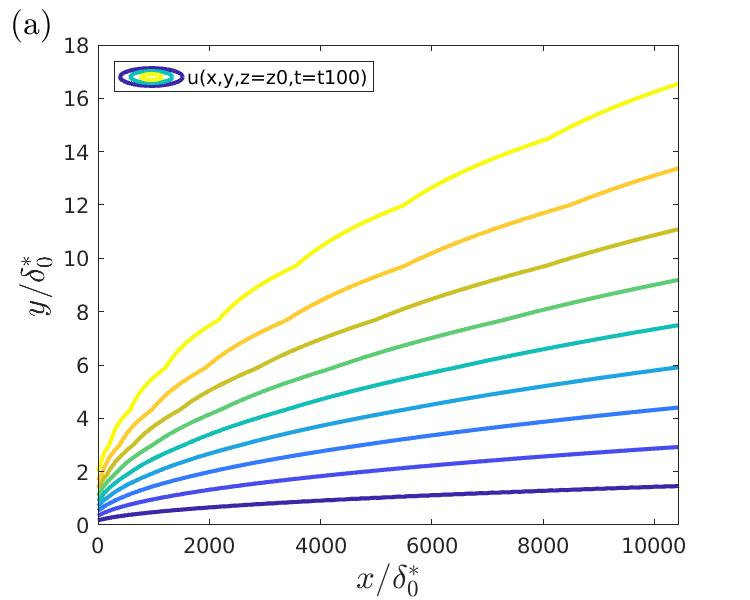
\includegraphics[width=0.49\textwidth ]{APG_laminar.jpg}
% 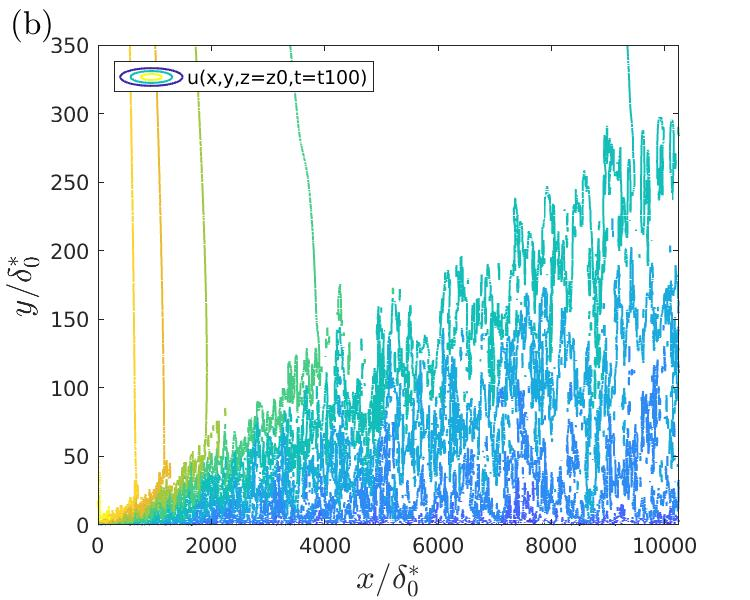
\includegraphics[width=0.49\textwidth]{APG_turb.jpg}
\caption{ \label{fig:lam_turb_development} Snapshot of the instantaneous streamwise velocity $u(\pmb{x})$ in 
\highlight{
(a) initial ZPG laminar flow-field used for the APG simulation and (b) turbulent APG boundary layer.
The contours are taken at $u=0.3, 0.5, 0.7, 0.9 U_0$, where $U_0=U_{\infty}(x=0)$ is a reference velocity.
The red line shows the thickness of the BL, $\delta_{99}$ where $u(y=\delta_{99})=0.99 U_{\infty}$ for the ZPG laminar case (a) and for the APG TBL in (b) the diagnostic plot method \cite{diagnostic_Vinuesa} is used. 
}   
}
\end{figure}



\section{Mathemathical analysis}

For an incompressible flow the conservation of mass in a control volume becomes the differential continuity equation:

% Continuity
\begin{equation}
\label{eq:continuity_cap2}
% \overrightarrow{u}
    \nabla \cdot \pmb{u} = \partial_i u_i = 
    \frac{\partial u}{\partial x} + \frac{\partial v}{\partial y} + \frac{\partial w}{\partial z} = 0,
\end{equation}
which is shown as the divergence of the velocity vector, in the diadic and components notations.
To describe the time evolution of the flow variables, it is possible to use the partial differential equations in Eq.~(\ref{eq:NS_cap2}), which are are the Navier--Stokes (NS) equations, and they describe the evolution of the momentum of the flow as a function of the pressure gradient and viscous forces acting on it. The system of equations comprising Eqs.~(\ref{eq:continuity_cap2}) and (\ref{eq:NS_cap2}) is valid for both laminar and turbulent-flow regimes, depending on the configuration of the problem.

% NS Total velocities
\begin{equation}
    \label{eq:NS_cap2}
    \frac {\partial u_i} {\partial t}  + u_j \frac {\partial u_i} {\partial x_j} =
    -\frac {1} {\rho} \frac {\partial p} {\partial x_i} +  \nu \frac {\partial^2 u_i} {\partial x_j^2}.
\end{equation}

By providing boundary conditions (BCs) together with an initial state of the system and the flow properties, we can expect either laminar, transitional or turbulent flow.
Once turbulence is developed, the statistical approach to turbulence is based on the Reynolds decomposition \citep{Rey_decomp}, given in Eq.~(\ref{eq:Rey_decomp}). This decomposition is based on a constant or averaged component and a fluctuating component in a way that once they are introduced into Eqs.~(\ref{eq:continuity_cap2}) and (\ref{eq:NS_cap2}) some of the terms are simplified. An example is to use a constant base flow (such as the laminar state) plus a fluctuating flow field, which is the case used to study transition and stability of BLs. 
For our case, the mean flow $U_i$ is an average in time and the homogeneous directions. The average in a dimension $d$ is marked as $\langle . \rangle_d$, and the average in time and all the homogeneous dimensions is marked with $\overline{(.)}$. In a spatially-developing boundary layer the mean velocity is $U_i = \overline{u_i} =\langle \langle u_i \rangle_z \rangle_t$ and as a result of Eq.~(\ref{eq:Rey_decomp}), $\overline{u_i\myprime}=0$. 
% Note that $\langle u_i\myprime \rangle_z (t) \neq 0$ and $\langle u_i\myprime \rangle_t(z) \neq 0$. 

Introducing the flow decomposition Eq.~(\ref{eq:Rey_decomp}) into the continuity and NS equations (\ref{eq:continuity_cap2}) $\&$ (\ref{eq:NS_cap2}), and using the average in time and $z$, we see that the continuity equation is fulfilled for both the mean and the fluctuating component separately, see Eq.~(\ref{eq:cont_decomp}). And in the momentum equations we obtain the Reynolds-averaged Navier--Stokes equation (RANS) in Eq.~(\ref{eq:RANS_cap2}) and the equation for the time evolution of the perturbations Eq.~(\ref{eq:pertub_cap2}) as a result of substracting the RANS equations from the general NS equations.

% R Decomposition
\begin{equation}
    \label{eq:Rey_decomp}
    u_i = U_i + u_i\myprime.
\end{equation}

\begin{equation}
    \label{eq:cont_decomp}
    \partial_i \overline{u_i} = \partial_i \overline{U_i} = 0 ,~~~~
    \partial_i \overline{U_i} + \partial_i \overline{u_i\myprime} = 0.  
\end{equation}

% RANS
\begin{equation}
    \label{eq:RANS_cap2}
    U_k\pdv{U_i}{x_k} + \pdv{\overline{u_i\myprime u_k\myprime}}{x_k} = -\frac {1} {\rho} \frac {\partial P}{\partial x_i} + \nu  \frac {\partial^2 U_k} {\partial x_k^2}.
\end{equation}

% Perturbations
\begin{equation}
    \label{eq:pertub_cap2}
    {\pdv{u_i\myprime}{t} + 
    U_k\pdv{u_i\myprime}{x_k} + u_k\myprime\pdv{U_i}{x_k} + u_k\myprime\pdv{u_i\myprime}{x_k} - \pdv{\overline{u_i\myprime u_k\myprime}}{x_k}  =
    -\frac{1}{\rho} \pdv{p\myprime}{x_i} + \nu  \frac {\partial^2 u_k\myprime} {\partial x_k^2}    }.
\end{equation}

Note that the RANS equations are similar to the NS equations, with the exception of the time derivative which is zero and it has an additional term $\pdv{\overline{u_i\myprime u_k\myprime}}/{x_k}$ which can be included within the divergence of the viscous-forces term, for that reason the terms in the tensor $\rho \overline{u_i\myprime u_k\myprime}$ are called Reynolds stresses. In the following, since the density is considered as constant, we will use the term Reynolds stresses (RS) for the terms in the tensor $\overline{u_i\myprime u_k\myprime}$, which are also known as the variance or covariance of the total velocities.
From the RANS equations it is interesting to analyze the mean velocities and the RS terms since they are an indicative of the level of turbulence and how it is affected by the pressure gradients and viscous forces on the right-hand side (RHS) of the equation.

The equation for the perturbation velocities is useful since we can multiply by another perturbation velocity such as $u_{j}\myprime \cdot \left( \pdv{u_{i}\myprime}{t} + ... \right) $ or obtain the two-point correlation $\mathcal{R}_{u_i\myprime u_j\myprime}$ through the correlation denoted with the symbol $(\cdot \star \cdot)$ as in $ u_{i}\myprime \star \left( \pdv{u_{j}\myprime}{t} + ... \right)$. The former gives the Reynolds-stress transport equations (\ref{eq:RS_transport_cap2}) where the turbulent kinetic energy budgets are a special case. The latter is used as in \cite{lee_moser_2019}, to obtain the power-spectral density of each term of the Reynolds-stress transport equations.

Denoting Eq.~(\ref{eq:NS_cap2}) as $\mathrm{TOT}_i$, Eq.~(\ref{eq:RANS_cap2}) as $\mathrm{RANS}_i$ and Eq.~(\ref{eq:RS_transport_cap2}) as $\mathrm{PERT}_i$, the evolution equation for the total kinetic energy of the flow can be obtained through the multiplication:
% $\mathrm{KE} = (1/2) \overline{u_i \cdot \mathrm{TOT}_i}$, 
\begin{equation}
    \mathrm{KE} = (1/2) \overline{u_i \cdot \mathrm{TOT}_i}, 
\end{equation}
while the mean kinetic energy equation can be obtained with:
% $\mathrm{MKE} = (1/2) U_i \cdot \mathrm{RANS}_i$,
\begin{equation}
    \mathrm{MKE} = (1/2) U_i \cdot \mathrm{RANS}_i,
\end{equation}
and the turbulent kinetic energy equation with 
\begin{equation}
    \mathrm{TKE} = (1/2) \overline{u_i\myprime \cdot \mathrm{PERT}_i} = \mathrm{KE} - \mathrm{MKE}.
\end{equation}
In a similar way the Reynolds-stress transport ($\mathrm{RST}_{ij}$) equation Eq.~(\ref{eq:RS_transport_cap2}) can be obtained by doing: 

\begin{multline}
    \mathrm{RST}_{ij} = \overline{u_i\myprime \cdot \mathrm{PERT_j} + u_j\myprime \cdot \mathrm{PERT_i}} = \\
    = \overline{u_i \cdot \mathrm{TOT_j} + u_j \cdot \mathrm{TOT_i}} - (U_i \cdot \mathrm{RANS}_j + U_j \cdot \mathrm{RANS}_i ) .
\end{multline}
In index notation, this yields:

% RS transport equation
\begin{multline}
    \label{eq:RS_transport_cap2}
    \pdv{\overline{u_i\myprime u_j\myprime}}{t} + 
    U_k\pdv{\overline{u_i\myprime u_j\myprime}}{x_k} + 
    \left(
    \overline{u_i\myprime u_k\myprime}\pdv{U_j}{x_k} + \overline{u_j\myprime u_k\myprime}\pdv{U_i}{x_k}
    \right) +
    \left(
    \overline{u_i\myprime \pdv{u_j\myprime}{x_k} u_k\myprime} + \overline{\pdv{u_i\myprime}{x_k} u_j\myprime u_k\myprime}
    \right)
    = \\ 
    - \left( \overline{
    u_j\myprime \pdv{p\myprime}{x_i} + u_i\myprime \pdv{p\myprime}{x_j}
    } \right) 
    + \nu \frac{\partial^2 \overline{u_i\myprime u_j\myprime}}{\partial x_k^2} 
    - 2\nu \overline{\pdv{u_i\myprime}{x_k} \pdv{u_j\myprime}{x_k}}.
\end{multline}

The third term in Eq.~(\ref{eq:RS_transport_cap2}) is particularly interesting, since after some manipulation that term appears in the transport of $U_iU_j$ and the transport of $\overline{u_i\myprime u_j\myprime}$ with different signs. It is usually written on the right-hand side of the equation and is called ``Production'', since it subtracts energy from the mean flow and adds it to the perturbations.
The rest of terms are discussed in Appendix B from \textbf{Paper 1}.


%===============================================================================
\chapter{Effects of adverse pressure gradients in turbulent boundary layers}
%===============================================================================
%

\section{Turbulent Boundary layers under adverse pressure gradients}

A wall-bounded flow can see pressure gradients as a result of the curvature of the wall, but also as a result of a change in the direction/velocity of the outer flow $(U_{e}, V_{e}, W_{e})$. Turbulence is already a complex problem in a ZPG case with the only parameter being the Reynolds number (momentum/viscous forces), if another parameter such as pressure gradients is added, the complexity of the problem increases and it becomes difficult to distinguish what phenomena is caused by the $\Rey$ effects or by the PG history of the flow.
In order to properly study APG TBLs, first we should try to define a canonical simple case, that is a well-defined APG along the streamwise development of the TBL, this is what we refere as the PG history of the flow.
To address this problem, different pressure-gradient parameters have been defined in literature, such as the Rotta-Clauser PG parameter $\beta$, or a general $\Lambda_{inc}$ which in \cite{Gibis2019} is studied with different length and velocity scales.
In our simulations of moderate APGs we have used $\beta$ defined as
\begin{equation}
    \beta(x) = \frac{\delta^*}{\tau_w} \pdv{P}{x},
\end{equation}
where $\pdv{P}{x}$ is the averaged pressure-gradient, $\tau_w$ is the shear stress at the wall, and $\delta^*$ is the displacement thickness, which for an incompressible flow is defined as
\begin{equation}
    U_e \delta^* = \int_{0}^{\delta_{99}} (U_e - U) dy
\end{equation}

% IDEA behind beta
The idea behind the $\beta$ parameter is to stablish an integral equilibrium of forces across the TBL, in this way, every section of the TBL is subjected to the same dimensionless state of forces.
To clear this idea, Fig.~\ref{fig:scheme_beta} shows a scheme of a section of the BL, where the main forces are due to the streamwise pressure-gradient and the stress at the wall.

\begin{figure}
    \centering
    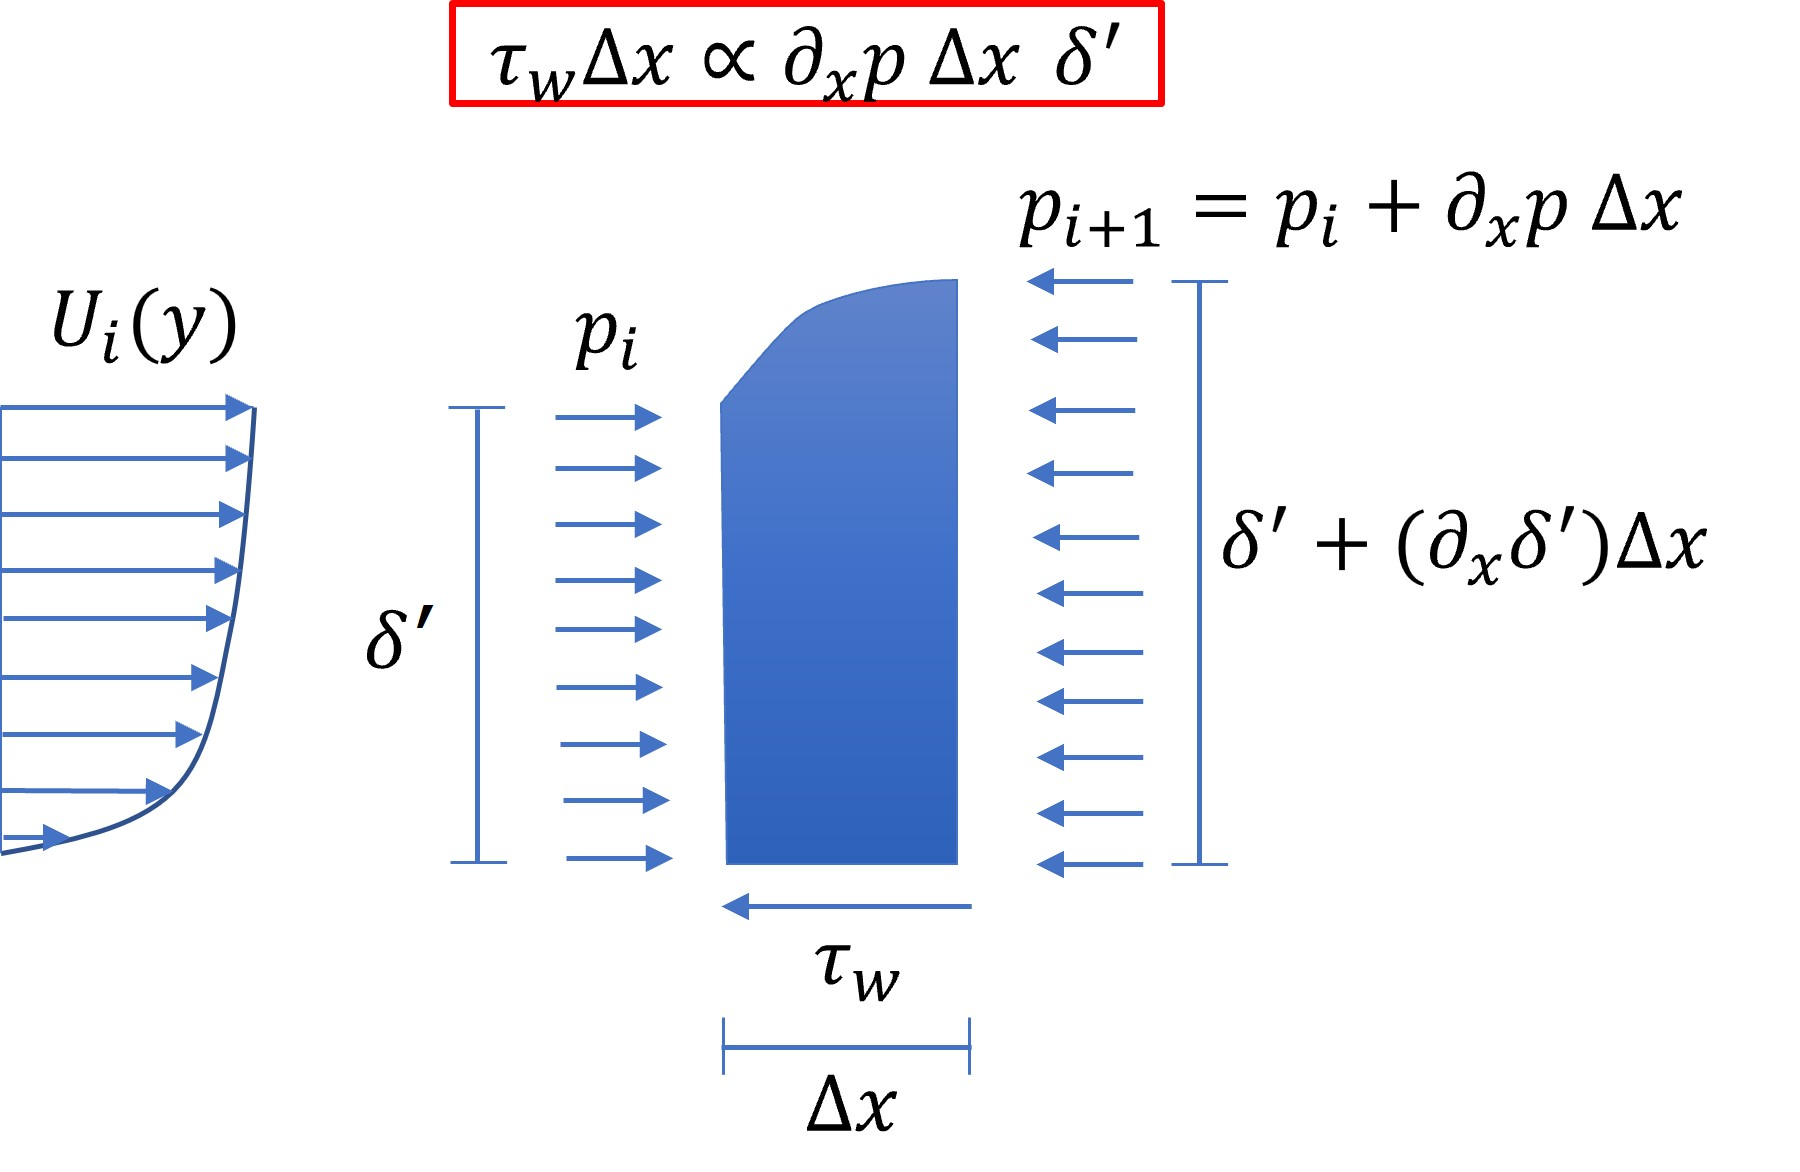
\includegraphics[width=0.90\textwidth]{imgs/schemes/scheme_beta.jpg}
    \caption{Stresses around a section of a BL.}
    \label{fig:scheme_beta}
\end{figure}

Integrating the streamwise momentum equation over the wall-normal direction, under several assumptions, it is possible to obtain an equation which relates the integral parameters $\delta^*$, $\theta$ and $\beta$, therefore, from an integral approach, the thickness $\delta \myprime$ is chosen equal to $\delta^*$. 



\section{Statistics}
In \textbf{Paper 1} we explore the statistical quantities of TBLs under APGs. The novelty respect to the available literature was in the high fidelity database used for the ZPG and APG TBLs. Both simulations show the development of the TBL from low Reynolds numbers such as those of previous numerical databases, and reach large Reynolds numbers such as those obtained in experiments. This characteristic works as a bridge to validate previous simulations as well as the current simulations, since they have been compared successfully with experimental data.
A benefit of numerical experiments is that the amount of quantities measured are larger than in experimental databases. This allows to have better measurements close to the wall and obtain decomposition such as spanwise spectra.

In Fig.~\ref{fig:U_uu_cap2}(a) we show the inner scaled $U$ and $\sqrt{\overline{u\myprime u\myprime}}$ for a $\Rey_{\tau}=500$, where the low Reynolds number simulations are already fully developed, while the experimental database does not have measurements. A higher $\Rey_{\tau}=2000$ is required by the experiments to have a fully developed near-equilibrium APG, and the LES ZPG and the new b1.4 simulation are able to achieve those Reynolds numbers.
The experimental data and b1.4 are in a similar range of $\beta$ and their statistics show a good agreement in the streamwise components.
The effects of the APG in $U$ show a lower $U^+$ for larger $\beta$ in the logarithmic region, and a larger effect in the wake region. At higher Reynolds numbers, the logarithmic region enlarges and the near-equilibrium APG and the ZPG profiles get closer.
In the turbulent perturbations, the near-wall or inner peak of $\sqrt{\overline{u\myprime u\myprime}}^+_{IP}$ grows in value with both the Reynolds number and the APG effects and its wall-normal position $y_{IP}^+$ seems to slightly increase with both APG and $\Rey$ effects. In \cite{Pozuelo_JFM_22} this trend is shown, where a filter was used to avoid saw-tooth jumps due to the wall-normal resolution close to the wall.
Larger Reynolds numbers allows for larger scales to live in the logarithmic/wake region and for a separation of the scales to be seen. This is first seen as lower decay in $\sqrt{\overline{u\myprime u\myprime}}$ in the ZPG in the logarithmic/wake region and a development of an outer peak for APG profiles. Larger $\beta$ increase the value of the outer peak of $\sqrt{\overline{u\myprime u\myprime}}$. The trends for the outer peak value and wall-normal position of the RS,  $\overline{u\myprime u\myprime}_{OP}$ and $y_{OP}$ where analysed in \cite{Pozuelo_JFM_22}. 


\begin{figure}
    \centering
    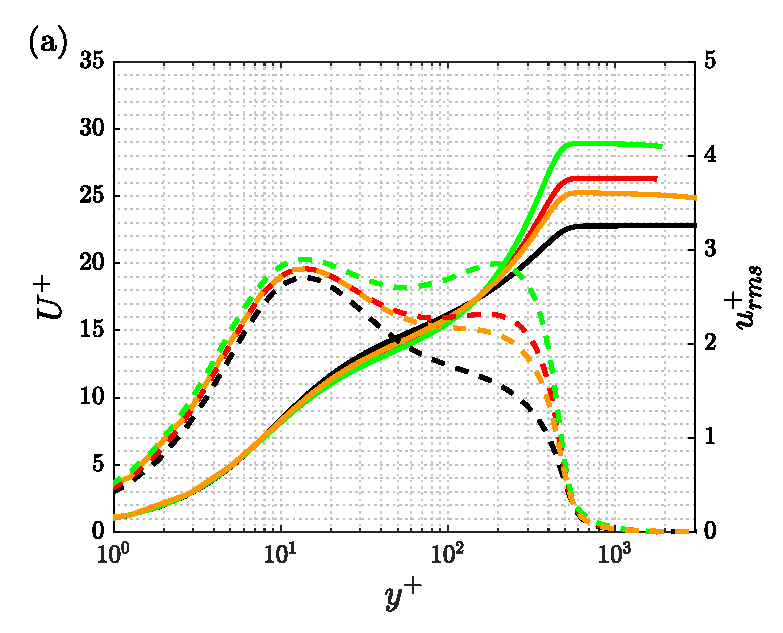
\includegraphics[width=0.49\textwidth]{imgs/stats/U_uu_a.eps}
    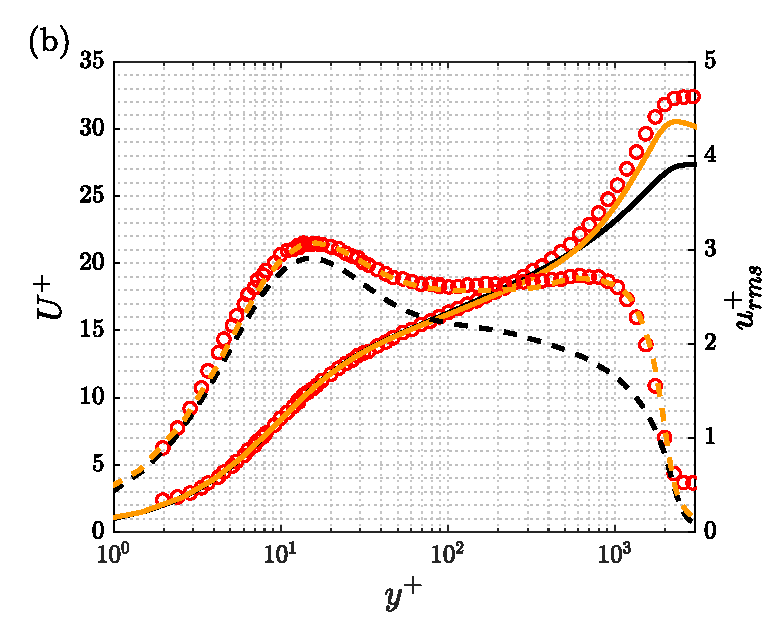
\includegraphics[width=0.49\textwidth]{imgs/stats/U_uu_b.eps}
    \caption{Mean streamwise $U$ (solid lines) and streamwise root mean square $u_{rms}$ or strandard deviation of the streamwise velocity (dashed lines). Wall-normal profiles taken at: (a) $\Rey_{\tau}=500$, (b) $\Rey_{\tau}=2100$. }
    \label{fig:U_uu_cap2}
\end{figure}

\subsection{Cf}

\subsection{RS}


\subsection{Spectral decomposition}
To have a better understanding on the perturbations we can use some mathematical tools such as the decomposition of the spatial-temporal signal using correlations, orthogonal modes, coherent structures, etc.
The use of orthogonal modes allows to decompose the energy of the perturbations into each mode in an unique way, so the sum of the energy contained in all the modes is equivalent to the total energy of the perturbations. 

In signal analysis an orthogonal decomposition which is commonly used is the Fourier decomposition which enables to look for phenomena that repeats with a certain time or spatial frequency. The energy or power associated with each mode is called energy spectra (if the signal is finite such as pulses) or power spectra (if the signal is such as sinusoidal waves, whose domain and energy is not finite, however its power is). Remember that the power is the ratio of the energy over time, where the time goes to infinity (in the case of using temporal series).
Since we are dealing with signals which are periodic in the homogeneous dimension $z$ and are not limited in time, we will use the terminology of power spectra (PS) instead of energy spectra. 
The modes in $z$ have a wavenumber $k_z$ and a wavelength $\lambda_z=2\pi/L_z$ where $L_z$ is the spanwise period of the domain. The same analysis can be applied in time, where we will use $k_t$ and $\lambda_t$.
For a signal $x(t)$, with $X(k_t)$ being its Fourier transform, the power of each mode is $|X(k_z)|^2$, the squared amplitude of the mode. For a perturbation velocity, the power can be calculated as,
\begin{equation}
    PS_{u_i\myprime u_j\myprime}(k_z) = \mathcal{F}(u_i \myprime)  \mathcal{F}^*(u_j \myprime),
    \label{eq:power_sp}
\end{equation}
where $\mathcal{F}()$ is the Fourier transform and $\mathcal{F}^*()$ represents the complex conjugate and the definition has been expanded to include the power spectra of the quantity $\langle u_i\myprime u_j\myprime \rangle_{z}$, also known as cospectra.
Using the properties of the Fourier transform, the multiplication in Fourier space represented in Eq.~\ref{eq:power_sp} represents the Fourier transform of the two-point correlation function $\mathcal{R}_{u_i\myprime, u_j\myprime}(\delta z)=u_i\myprime \star u_j\myprime$, where $\delta z$ is the lag or distance between the two points where we look for the correlation of their velocity perturbations. According to the Wiener--Khinchin theorem, we can calculate the PS through as the Fourier transform of $\mathcal{R}_{u_i\myprime, u_j\myprime}$ or from the power spectra throught the inverse Fourier transform $\mathcal{F}^{-1}()$ we can obtain the two-point correlation function.

Note that for velocity perturbations, since Fourier modes are orthogonal, the sum of the PS for all the modes is equal to the averaged Reynolds stress,
\begin{equation}
    \langle u_i\myprime u_j\myprime \rangle_{z} = \sum_{k_z} PS_{u_i\myprime u_j\myprime}(k_z)
\end{equation}

This step can be performed for each time step and averaged over time to obtain $\langle\langle u_i\myprime u_j\myprime \rangle_{z}\rangle_{t} = \overline{u_i\myprime u_j\myprime}$ or it can also be the result of a 2D spectral decomposition in both time and $z$, where the sum extends to all the spatial and temporal modes.

The PS is useful for discrete systems, and it is the first step when we calculate numerically the spectra of a the Reynolds-stresses. It is also interesting to see how the power spectra is distributed along the wavenumbers or the wavelengths, obtaining a power spectral density (PSD).
The average in time of the PSD in wavenumbers is $\phi_{u_i\myprime u_j\myprime}=\langle PS \rangle_t/\mathrm{d} k_z$ while the average in time PSD in wavelengths is $\psi_{u_i\myprime u_j\myprime}= \langle PS \rangle_t/\mathrm{d} \lambda_z$. Both densities can be linked using $\mathrm{d}(\lambda_z) = \mathrm{d}(2\pi/k_z) = -2\pi\mathrm{d}k_z/k_z^2$:

\begin{equation}
    \psi_{u_i\myprime u_j\myprime} = 
    \frac{ \langle PS_{u_i\myprime u_j\myprime} \rangle_t}{\mathrm{d} \lambda_z} =
    -\frac{ \langle PS_{u_i\myprime u_j\myprime} \rangle_t}{\mathrm{d} k_z} \frac{k_z^2}{2\pi},
\end{equation}
where the minus sign is taking care by inverting the limits of integration to obtain the total RS (small to large wavenumbers is equivalent to integrate from large to small wavelengths).

\begin{equation}
\label{eq:sum_ps}
    \overline{u_i\myprime u_j\myprime} = 
    \int_{k_z=k_0}^{k_z=k_{N}}   \phi_{u_i\myprime u_j\myprime}  ~ \mathrm{d} k_z =
    \int^{\lambda_z = 2\pi/k_0}_{\lambda_z = 2\pi/k_{N}}  \psi_{u_i\myprime u_j\myprime}  ~ \mathrm{d} \lambda_z
\end{equation}

In Fig.~\ref{fig:PS_PSD} we show for a ZPG TBL, different representations of the PSD of $\overline{u\myprime u\myprime}$ where the image with the black contours represent a streamwise profile at $\Rey_{\tau}=2000$ while the red contours are taken at a position where $\Rey_{\tau}=500$.

\begin{figure}[h!]
\centering
% \captionsetup{width=0.99 \textwidth}
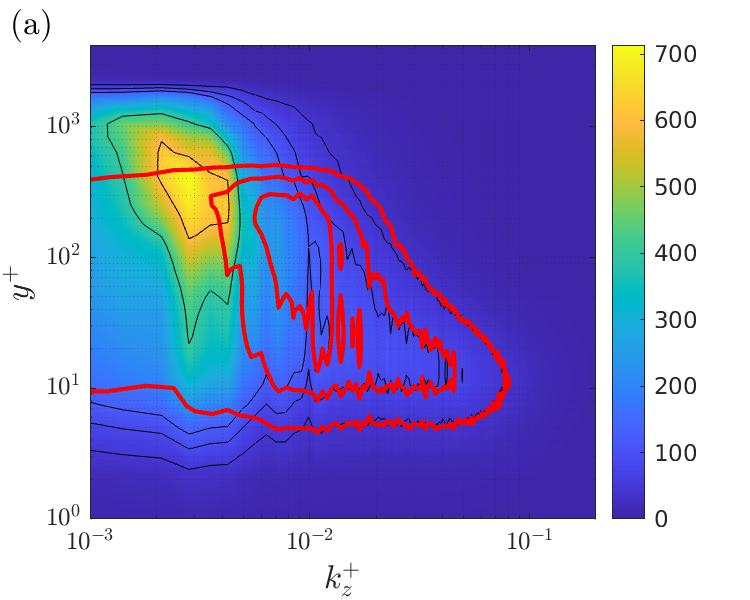
\includegraphics[width=0.32\textwidth ]{imgs/spec/ZPG_Ret_500_2000_PSdkz_kz_ltau_y_ltau.jpg}
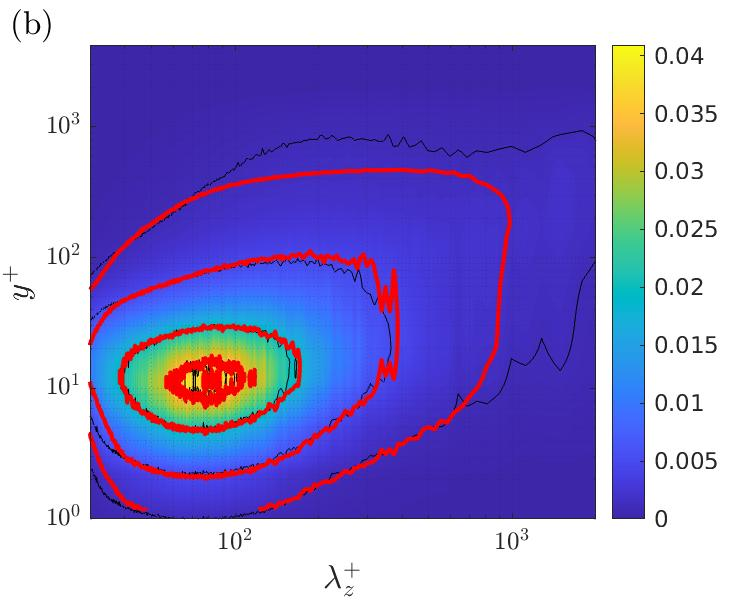
\includegraphics[width=0.32\textwidth]{imgs/spec/ZPG_Ret_500_2000_PSdlambdaz_lambdaz_ltau_y_ltau.jpg}
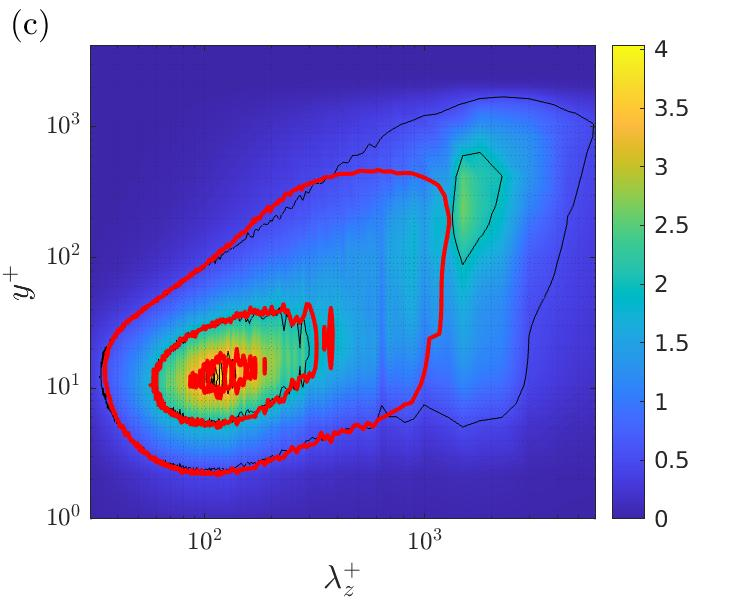
\includegraphics[width=0.32\textwidth]{imgs/spec/ZPG_Ret_500_2000_kPSdkz_lambdaz_ltau_y_ltau.jpg}
\caption{ \label{fig:PS_PSD} Spanwise spectra of the streamwise Reynolds stress $\overline{uu}(y)$. (a) Power spectral density $\phi_{u\myprime u\myprime}(y,k_z)$; (b) Power spectral density $\psi_{u\myprime u\myprime}(y,\lambda_z)$; (c) premultiplied power spectral density $k_z\phi_{u\myprime u\myprime}$. Wavenumbers, wavelengths, wall-normal position and power spectra scaled in viscous units.}
\end{figure}
% contours: Retau 2000: [40 80  120 400 600]; [0.001 0.005 0.02 0.035 0.04] ;  [ 0.5 2 3.5]; 
% contours: Retau  500: [40 80  120        ]; [0.001 0.005 0.02 0.035 0.04] ;  [ 0.5 2 3.5]; 

The PS and the PSD in the wavenumbers $\phi_{u\myprime u\myprime}(y,k_z)$ present the same features as in Fig.~\ref{fig:PS_PSD}(a), since $dk_z$ or $dk_z^+$ are constant factors that does not vary with the wavenumbers. It shows a high content of power/energy of structures with a very low wavenumber which are very wide. It is possible to see similarities in the contours at different Reynolds numbers (red and black lines) in the region of high wavenumbers (small scales), although the energetic level is very low compared to that of the low wavenumbers (large scales).
The PSD in wavelengths $\phi_{u\myprime u\myprime}(y,\lambda_z)$ is represented in Fig.~\ref{fig:PS_PSD}(b) and it focuses on the small scales. It shows that the density of power/energy in the small scales (short wavelengths) is very similar at different Reynolds numbers and larger than the PSD of the wider scales (large $\lambda_z^+$). 
From Fig.~\ref{fig:PS_PSD}(a) and (b) we see that the small scales have a small content of the total RS energy, but their small size make the density in waveleghts to be very concentrated, while for the wider scales is the opposite, the energy they contain is very large, but their big size make the PSD to be very low or disperse.
If we write both PSD as a function of $\phi_{u\myprime u\myprime}$, in Fig.~\ref{fig:PS_PSD}(a) we show $\phi_{u\myprime u\myprime}$ while in Fig.~\ref{fig:PS_PSD}(b) it would be $k_z^2 \phi_{u\myprime u\myprime}$, the premultiplication factor $k_z^2$ is responsible to augment the effects of the small scales while diminishing the effects of the large scales. Fig.~\ref{fig:PS_PSD}(c) shows $k_z \phi_{u\myprime u\myprime}$, whose effect equilibrates the effect of the large and small scales obtaining a better visualization of both scales.

The premultiplied PSD $k_z \phi_{u\myprime u\myprime}$ is widely used and it has a geometrical explanation.
Since the range of energetic scales is so large that we observe very small scales close to the wall and very large scales of the size of $\delta_99$, the use of logarithmic axis helps to expand the region of small $\lambda_z$ and the region close to the wall.
If we use logarithms in the definition of wavelength, $ \mathrm{ln}(\lambda_s) = \mathrm{ln}(2\pi) - \mathrm{ln}(k_z)$, and apply the differential, $\mathrm{d}(\mathrm{ln} \lambda_z) = -\mathrm{d}(\mathrm{ln} k_z)$, and together with $\mathrm{d}k_z = k_z \mathrm{d}(\mathrm{ln} k_z)$ can be substituted in Eq.~\ref{eq:sum_ps} to obtain:
\begin{equation}
    \overline{u_i\myprime u_j\myprime} = 
    \int_{k_0}^{k_{N}}   \phi_{u_i\myprime u_j\myprime}  ~ \mathrm{d} k_z = 
    \int_{k_0}^{k_{N}}   \phi_{u_i\myprime u_j\myprime} k_z  ~ \mathrm{d}( \mathrm{ln} k_z) = 
    \int^{\lambda_0}_{\lambda_{N}}   \phi_{u_i\myprime u_j\myprime} k_z ~ \mathrm{d}( \mathrm{ln} \lambda_z).
\end{equation}

The premultiplication by $k_z$ can be seen here as a factor to visualize a corrected area after scaling the axis with a logarithmic scale.
From here on the PSD will always be represented in its premultiplied form $k_z\phi$ to have a clear visualization of the effects of large and small scales at the same time.

\subsubsection{Wide scales in turbulence. Channel Flows}
It has been seen that the big scales contains a large part of the turbulent energy, although the density spectral density is low.
When we model the turbulent flow, the size of the domain imposes a limit on the size of the scales that can be simulated. In a periodic domain, the largest scale corresponds to $L_x$ and the wider scale to $L_z$. Bigger scales will be seen as infinit in size because of the periodicity, and the spectral energy will be stored in the zero-wavenumbers.

The energy contained in the zero-wavenumbers is affected by the averaging.

If the size of the domain is not large or wide enough, the bigger turbulent scales will not be able to be captured and the energetic spectrum will not be correct, affecting the total statistics such as the Reynolds stresses and the mean velocity profiles.
Many analysis on the size of the domain has been performed on canonical turbulent channel flows for it simplicity.
\highlight{Minimal channels are those small domains that assure }
On the other way, the largest scales in channel flows where looked for in \highlight{CITAR ADRIAN que descubrieron bla bla}.
The study on the wider scales was based on two-point correlations, but no other study similar to \highlight{CITAR ADRIAN} was performed in the spanwise direction.

To have a better understunding of the wide scales obtained in APG TBLs and the effects of the domain size, we decided to study first the effect on wide-channels.
Three simulations were performed of turbulent channel flows at $\Rey_{\tau} = 550 $ under similar conditions, with the only excemption the width of their domains which was doubled from one channel to another as it can be seen in \highlight{Tabla de los channel}.
 


\subsubsection{Spectral results on APG}

In \textbf{Paper 1} the 1D spanwise spectra and the 2D spanwise and temporal spectra of the APG TBL where shown and compared to those of a ZPG TBL \citep{EAmorZPG}. By using percentage contours it was possible to show a similar behaviour in the mild APG and the ZPG simulations at different Reynolds numbers in the small-scale energy region close to the wall around an spectral near-wall peak or spectral inner peak (sIP) at $y^+\approx 15$ and $\lambda_z^+\approx 120$. Another region with similar shape is in the wake region with an spectral outer peak that seemed to scale with the Reynolds number.
Another region is that of small-scale energy in the wake region, which is only present in the APG simulation and not in the ZPG case.

\begin{itemize}
    \item show pcolor con APG y ZPG de uu, uv en Retau 500 y 2000
\end{itemize}

The spectra shows a similar region of small-scale energy close to the wall which is responsible of the near-wall peak the RS $\overline{u\myprime u\myprime}$. The effects of $\Rey$ and $\beta$ increase the value of $\overline{u\myprime u\myprime}_{IP}^+$, even if the most of the spectra is similar for APG and ZPG at different Reynolds numbers.
The outer-spectral peak in $k_z\phi_{uu}$ is also responsible of most of the energy contained in the ZPG in the wake region, and increasing $\beta$ it increases the energy to the point of growing the outer peak in $\overline{u\myprime u\myprime}_{OP}^+$. This behaviour is similar in the other components of the RS tensor, where at higher $\Rey$ numbers there are larger and energetic scales acting on the wake region and influencing all across the TBL.

\subsubsection{Scaling of APG spectrum}

In \textbf{Paper 2} we try to understand the trends of the inner and outer peaks in $\overline{u\myprime u\myprime}$ shown in \textbf{Paper 1}. Why the inner scaled inner-peak grows with the Reynolds numbers and with the APG effects. Is it still correct to use viscous scaling?. 
We perform a scaling analysis of the different energetic scales of the power spectral density for both ZPG and APG simulations and at different Reynolds numbers.
First we start from the features observed in $k_z\phi_{u\myprime u\myprime}$ which are an spectral near-wall/inner peak (sIP) and an spectral outer peak (sOP). The data is scanned to look for the maxima at a certain wall-normal position and the maxima at a certain frequency. Since $k_z\phi_{u\myprime u\myprime}$ is saved in a rectangular matrix, it is equivalent to obtain the maxima along columns and the maxima along rows.
At high Reynolds number the separation of scales even in ZPG TBLs, allows to distinguish clearly the presence of 2 maximal points for $\Rey_{\tau}>500$. Other techniques could be used to detect the local maxima, but this method was obtaining satisfactory results, specially the values of $f(y)=max(k_z\phi(k_z, y))_{k_z}$ since that function presents less noise and it is shown in \highlight{ Fig.~\ref{fig:scaling_OP} figura de los escalados de los picos} that once the Reynolds number is enough to have separation of scales, the outer peak clearly separates in the wall-normal direction from the spectral near-wall peak.
Once sIP and sOP are located in $k_z\phi(k_z, y)$, (usually we represent with $\lambda_z$), we try the inner and outer length scalings used in \textbf{Paper 1} to scale $\overline{u\myprime u\myprime}(y)$.
It is shown that the viscous length $\ell_{\tau}$ scales the size of the spanwise scales of the sIP $\lambda_{z, sIP}^+$ as well as the wall-normal position $y^+_{sIP}$.
The same method is used for the spectral outer peak. The outer scales $\delta^*$ and $\delta_{99}$ were used to scale independently the wall-normal location $y_{sOP}$ and the size of the scales $\lambda_{z, sOP}$.
In previous studies such as \cite{Kitsios2017} the $\delta^*$ scaling was successful for the $y_{OP}$ as well as for $y_{sOP}$ at much higher $\beta$, however, $\lambda_z$ was also scaled with the same scaling.
In \cite{tanarro_2020}, the outer scaling was performed with $\delta_{99}$ for both $y$ and $\lambda_z$, and the values of $\lambda_{z,sOP}$ were better collapsed than using $\delta^*$ as in \cite{Kitsios2017}.
Taking into account this previous studies, we allowed $y$ and $\lambda_z$ to have different length scalings, and found the optimal collapse of the region around the spectral outer peak using $y/\delta^*$ and $\lambda_z/\delta_{99}$.

Once we obtained the scalings for the wall-normal position and size of the scales for both sIP and sOP, we looked the region around those peaks using the respective scalings, obtaining a good collapse, however there was another region to investigate, which is the region of small-scale energy in the wake region.
Different scalings were tried for $\lambda_z$ looking to match the vertical part of the energetic contours of the APG simulation at different $\Rey$.
We observed that using $\lambda_z/\delta^*$, there is a collapse around $\lambda_z/\delta^*=0.3$. It could be argued that the scaling evolves gradually at different $\lambda_z$ up to the region around the sOP that clearly scale using $\lambda_z/\delta_{99}$.
To have a better idea of how big was the contribution of the small-scale energy in the wake region, but also to understand what is the influence of the large scales in the near-wall region, we tried to accumulate the energy from small to large scales for all the wall-normal positions. In a matrix containing the $PS(y,k_z)$, this is equivalent to do a cumulative sum $cumsum(PS(y,k_z))_{k_z}$ along $k_z$.
In \cite{EAmorZPG}, they limited a rectangular region around sIP, to probe that inner scaled energy in this region does not vary with the Reynolds number, but we have seen that there are different scalings at different heights of the TBL, therefore, the rectangular domain to integrate over $\lambda_z$ and $y$ may not be the optimal tool for this analysis.

With the idea of looking for the contribution of small and large scales using a cumulative sum, and thinking that the accumulated energy would be in a certain scaling that probably would change with $\Rey$ effects, we thought of the percentual contribution of energy, or the marginal contribution of energy.
For a continuous PSD, the marginal contribution of energy (MCE) is defined as in Eq.~\ref{eq:MCE_cap2} and gives the percentual level of energy added by scales up to a wavenumber $k_{z,c}$ respect to the total value which would be $\overline{u_i\myprime u_j\myprime}$ at the same $y$.

\begin{equation}
\mathrm{MCE} = \int_{k_{z,c}}^{\infty} \phi_{u_iu_j} \mathrm{d} k_z \ \bigg/ \int_{0}^{\infty} \phi_{u_iu_j} \mathrm{d} k_z,
\label{eq:MCE_cap2}
\end{equation}

If we draw the $10\%, 20\%,...,$ contours, it is easy to show the regions where certain election of length and energy scales are valid, since the contours will be parallel where the scales contributes in the same way to the total RS. And they will start to diverge when the scaling is not appropriate.
Where the scaling is independent of $\Rey$, the contours for different $\Rey$ at the same MCE level in that region, will collapse, otherwise they will start to separate indicating for example that the influence of large-scale motions is affecting that region.
All of this is shown in \textbf{Paper 2} in more detail.
Answering why $\overline{u\myprime u\myprime}_{IP}^+$ grows with the $\Rey$ and $\beta$, the answer is that at higher $\Rey$ the influence of scales of size $\delta_{99}$ or larger, influence the near-wall region, and this influence is larger at with larger $\beta$. At this range of $\beta$, the viscous scaling is still valid, although certain modifications could be done taking into account the influence of the large scales.
At larger $\beta$, the flow is near-detachment and the viscous scaling is no longer applicable.











%
%===============================================================================
\chapter{Transport of energy between turbulent scales}
%===============================================================================
%

\subsubsection{Interscale transport of energy.}

From the Reynolds transport equation or the KE, MKE and TKE budget equations, it was possible to obtain a term called ``Production'' which is composed by the RS and the mean velocity gradients, and it can be interpreted as a source of turbulent energy in the TKE equation and a sink in the MKE equation. Their contribution are cancelling each other when added to obtain the KE equation.

Following this idea, a similar term is looked for in the Reynolds-stress transport equations, that may indicate the transfer of energy between large scales and small scales.
In order to obtain such a decomposition, we follow the steps in \cite{PRL2018_Kawata, JFM2019_kawata_alfredsson}, where the perturbation velocity is further decomposed in a contribution from large scales $u_i^L$ and a contribution from small scales $u_i^S$, where the separation between large or small scales is made by a cutoff frequency/wavenumber in Fourier space $k_{z,c}$.
\begin{equation}
    \label{eq:intersc_decomp}
    u_i\myprime = u_i^L + u_i^S,
\end{equation}
\begin{equation}
    \label{eq:intersc_decomp}
    \langle u_i\myprime u_j\myprime \rangle_z = 
    \langle u_i^L u_j^L \rangle_z + 
    \langle u_i^S u_i^S \rangle_z
\end{equation}
\begin{equation}
    \label{eq:intersc_decomp}
    \overline{u_i\myprime u_j\myprime} = 
    \overline{ u_i^L u_j^L} + 
    \overline{ u_i^S u_i^S}
\end{equation}

\begin{equation}
    \label{eq:intersc_decomp}
    \overline{ u_i^L u_j^S} = 
    \overline{ u_i^S u_j^L} = 0
\end{equation}



\begin{itemize}
    \item 
\end{itemize}
%
%===============================================================================
\chapter{Numerical experiments on high Reynolds numbers flat plate turbulent boundary layers}
%===============================================================================
%
\section{SIMSON}

\section{Equations}



\section{MPI}


\section{LES}


\section{BCs}
%===============================================================================
\chapter{Conclusions and outlook}
%===============================================================================
%
%===============================================================================
% %===============================================================================

% This chapter is meant for testing the correct referencing of figures, equations
% and tables.

% % equations
% %
% \begin{equation}
% 	1 + 1 = 2
% 	\label{eq:test_eq1}
% \end{equation}

% \begin{align}
% 	2 + 2 = 4
% 	\label{eq:test_eq2}
% \end{align}

% \begin{equation}
% 	3 + 3 = 6
% 	\label{eq:test_eq3_intro}
% \end{equation}

% % tables
% %
% \begin{table}
% 	\centering
% 	\begin{tabular}{c}
% 		1
% 	\end{tabular}
% 	\caption{Test table 1}
% 	\label{tab:test_tab1}
% \end{table}

% \begin{table}
% 	\centering
% 	\begin{tabular}{c}
% 		2
% 	\end{tabular}
% 	\caption{Test table 2}
% 	\label{tab:test_tab2}
% \end{table}

% \begin{table}
% 	\centering
% 	\begin{tabular}{c}
% 		3
% 	\end{tabular}
% 	\caption{Test table 3}
% 	\label{tab:test_tab3_intro}
% \end{table}

% % figures
% %
% \begin{figure}[h!]
% 	\centering
% 	test figure 1
% 	\caption{Test figure 1}
% 	\label{fig:test_fig1}
% \end{figure}

% \begin{figure}[h!]
% 	\centering
% 	test figure 2
% 	\caption{Test figure 2}
% 	\label{fig:test_fig2}
% \end{figure}

% \begin{figure}[h!]
% 	\centering
% 	test figure 3
% 	\caption{Test figure 3}
% 	\label{fig:test_fig3_intro}
% \end{figure}

% test references
% %
% \hrule
% \begin{itemize}
% 	\item reference to equation 1: \eqref{eq:test_eq1}
% 	\item reference to equation 2: \eqref{eq:test_eq2}
% 	\item reference to equation 3: \eqref{eq:test_eq3_intro}
% \end{itemize}
% \hrule
% \begin{itemize}
% 	\item reference to table 1: \eqref{tab:test_tab1}
% 	\item reference to table 2: \eqref{tab:test_tab2}
% 	\item reference to table 3: \eqref{tab:test_tab3_intro}
% \end{itemize}
% \hrule
% \begin{itemize}
% 	\item reference to figure 1: \eqref{fig:test_fig1}
% 	\item reference to figure 2: \eqref{fig:test_fig2}
% 	\item reference to figure 3: \eqref{fig:test_fig3_intro}
% \end{itemize}
% \hrule

%===============================================================================
% Acknowledgments
%===============================================================================
%
\begin{acknowledgements}
% 	We would like to thank Gigi and SCIgen - An Automatic CS Paper Generator%
% 	\footnote{\url{https://pdos.csail.mit.edu/archive/scigen}}.
I would like to thank Ricardo Vinuesa and Philipp Schlatter first, without them I wouldn't have lived this wonderful adventure,
conducting my PhD studies in KTH and start a new life in a beautiful country such as Sweden.
To all those friends, old and new PhD students and professors that have made my stay so enjoyable.
And to my family in Spain and those that I got to consider family in Sweden for your support and love.
% Qiang Li, a collaborator in my publications, but also a mentor, always encouraging me and ready to help. They have helped and guided me through my academic work and have always been there to share their knowledge an experience.
% I also have to thank all those PhD's and professors that have made the life in the office so wonderful, in spite of the huge change that covid brought to our lifes.
% Luca, Simon, Valerio and Vitor, with whom I lived my first "western" adventure. And the list goes on and on.
% My family and friends in Spain that missed me so much, and my small "family" in Sweden for your moral support in good and dark times.
\end{acknowledgements}



%===============================================================================
% References
%===============================================================================
%
\bibliographystyle{jfm}
\bibliography{thesis}
%
% \IfFileExists{overview.bbl}{\graphicspath{{imgs/}}

%===============================================================================
\chapter{Introduction}
%===============================================================================
%
% Throughout my academic career, I have enjoyed the step-by-step process of learning and I have discovered a passion for sharing my knowledge with friends, colleagues and some of my students.
% In the same way the process of learning is unique, the process of teaching or communicating the knowledge should also be personal, trying to achieve the main goal of communication, transmitting correct information.
% When we try to learn about a subject we can go to books, classes, different teachers, publications..., and sometimes we understand better from a book, other times from a video or a specific teacher or friend.
% In this thesis, I will present some results on the physics of turbulent fluid mechanics where I have been involved, and I will try my best to communicate this knowledge to those interested in reading this work even if the reader is not very familiar with fluid dynamics.
% Ideally, this transmission of knowledge should be concise, but I have experienced that certain complex knowledge sometimes requires different points of view or a simpler language. Personally, I like to communicate my knowledge as if it was a conversation instead of formal and impersonal writing.

Fluid mechanics 
% or dynamics may sound as something complex for the non initiated, and 
it really is a complex science, but we already have intuitive and practical knowledge since we live and manipulate fluids every day 
% so I will
, so here we will
explain the basics.
A fluid is a substance that, in contrast to a solid, can easily deform and this property allows for the substance to adapt to containers or to move around other obstacles. An example is the air of the atmosphere, the liquid water in the sea, and even solids, like large accumulations of fine sand which subjected to vibrations can behave similar to liquid water.
Fluid mechanics is the science that studies everything related to the movement of fluids, like the forces involved or the properties of the fluid in its motion.

When a fluid moves around a solid (water around a rock), or the solid moves immersed in a fluid  (car moving through the air of the atmosphere) the fluid adapts to that relative motion by changing its properties, such as the velocity of its particles.
Where the fluid meets the solid, its particles have the same velocity as the solid because the forces in the interface fluid-solid (friction and pressure forces) are sufficient to deform the fluid.
The viscosity is the property of the fluid that opposes the deformation. Inside the fluid, the viscosity is seen as a force that reduces the velocity of the deformation or the velocity of the fluid particles.
In the example of the water in a river moving around a rock, far from the rock, the velocity of the water is that of the river, however the water in contact to the rock is not moving according to what was discussed earlier. The viscosity is responsible for adapting the velocity of the fluid from the velocity of the river to the velocity of the rock.
The change of velocity is actually done over a very small distance, and this region where the viscosity forces are adapting the fluid velocity is called boundary layer. 
The idea of the boundary layer was introduced by Ludwig Prandtl in 1904 and it is the main topic of this thesis.

The boundary layers studied here are those pertaining to the momentum of the flow. The interest is in the effects of adverse pressure gradients in fully-developed turbulent boundary layers. To avoid the influence of other effects we consider the simplest scenario.
The fluid is isotropic, incompressible and Newtonian, therefore the temperature does not change the density and the viscosity of the fluid.

The simplest solid boundary is a flat plate without any heat or mass exchange (no suction or blowing). The adverse pressure gradient is then imposed as an outer boundary condition.
Comparisons can then be done with curved-boundary solids such as NACA wing profiles, where the pressure gradients are caused by the curvature of the profile. 
In these more realistic configurations we consider various mechanisms to control the flow, such as blowing or suction.

For these simple configurations we use a Cartesian system of coordinates where the space is denoted with $\mathbf{x}=x_i=(x,y,z)$, which correspond to the vectorial, dyadic and coordinate notations that will be used in this work.
The boundary layers studied here are statistically two-dimensional (2D), $y$ is the wall-normal direction, $z$ is the homogeneous direction and $x$ is chosen as the streamwise direction. The time is denoted with $t$.
Although turbulence is a three-dimensional (3D) phenomenon, the flow under study is statistically 2D, since the $z$ direction is homogeneous.

%-------------------------------------------------------------------------------
\section{Our Contribution}
%
\thesisstructure Part I of the thesis contains 4 chapters. 
In chapter 2 we provide a basic introduction to fluid mechanics and turbulent boundary layers affected by adverse pressure gradients.
From the observations and expected phenomenology to the mathematical equations that describe the mechanics of the flow, and the equations that we use to approach the study of turbulent flows.
Chapter 3 introduces one of the biggest simulations on near-equilibrium turbulent boundary layers performed so far. The high-quality data on adverse-pressure gradient turbulent boundary layers is used to asses different phenomena such as the effects of adverse pressure gradients on the friction coefficient or the scaling factors of the turbulent scales using spectral decomposition.
Chapter 4 deals with the problem of the energetic exchange between turbulent scales, where we discuss the mathematical approach and its significance.
Finally in Chapter 5 we present the numerical code used for the simulations, and some details of the set up for the large simulation that we have presented.

%===============================================================================
\chapter{Boundary layers, turbulence and pressure gradients}
%===============================================================================
%
\graphicspath{{imgs/} {imgs/lam_turb} {imgs/spec}}

\section{Observations and empirical knowledge}

There are many examples of laminar and turbulent flows in nature that we are familiar with. In Fig.~\ref{fig:lam_turb} we show 3 examples, with water and flames. In the river image the water on the right side is laminar and on the left side it becomes turbulent. The calm flames of a candle rise initially in a laminar regime. On the bonfire example the flames are larger and show the different chaotic scale motions of a turbulent flow.

\begin{figure}[h!]
\centering
% \captionsetup{width=0.99 \textwidth}
% 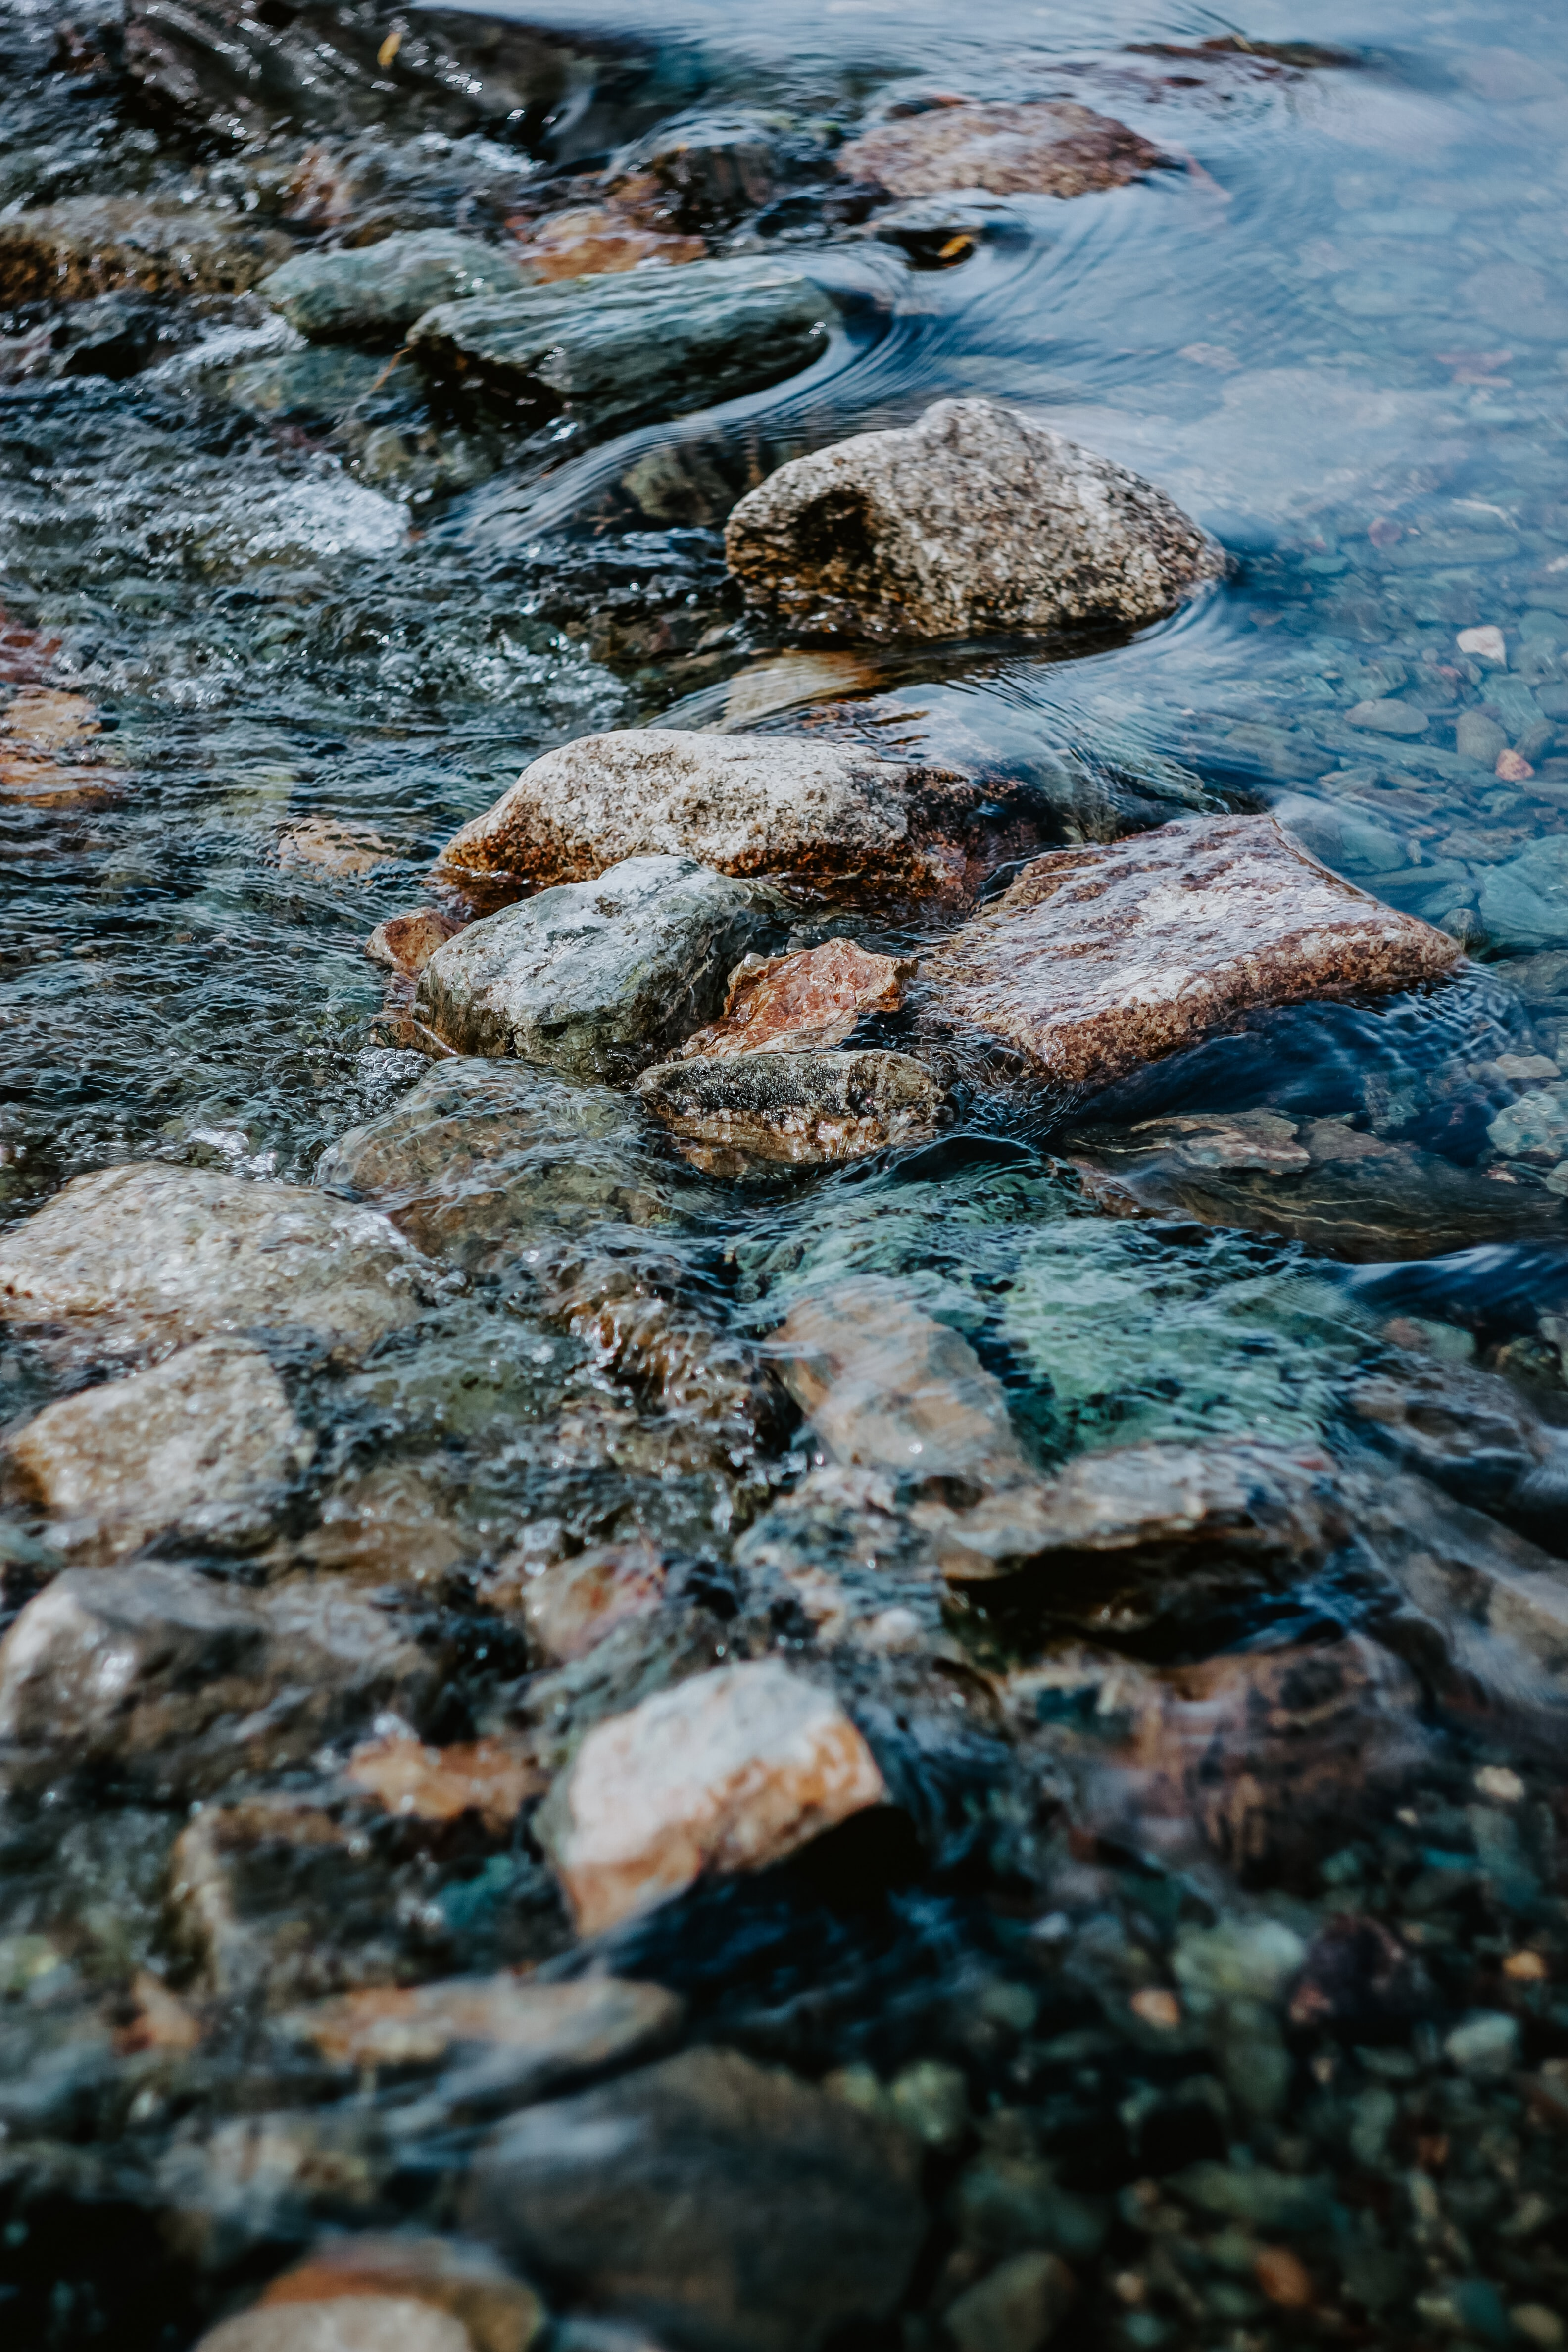
\includegraphics[height=5cm ]{laminar_turbulent_1.jpg}
% % 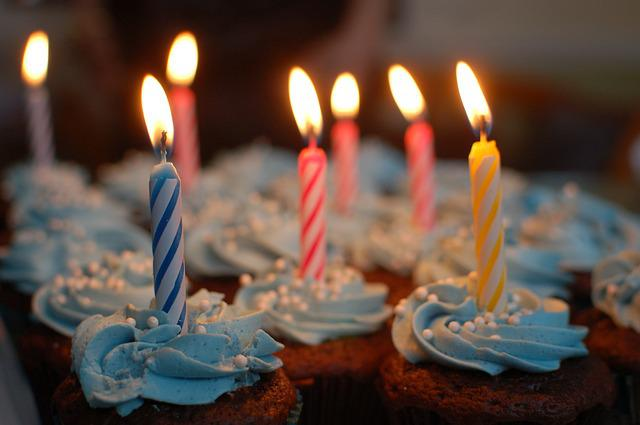
\includegraphics[width=5cm ]{llama_laminar.jpg}
% 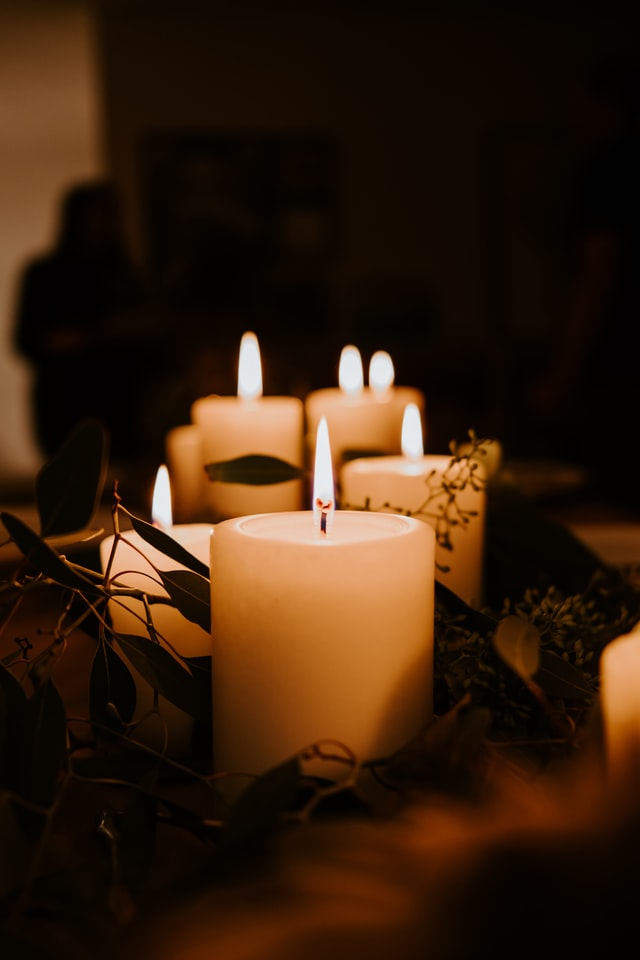
\includegraphics[height=5cm ]{velas.jpg}
% 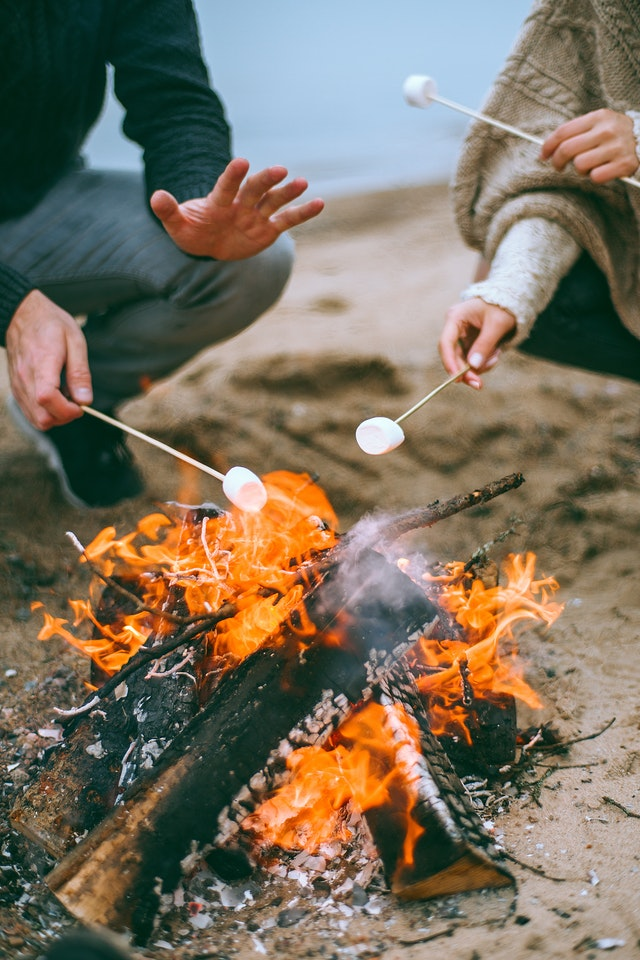
\includegraphics[height=5cm ]{llama_turb1.jpg}
% 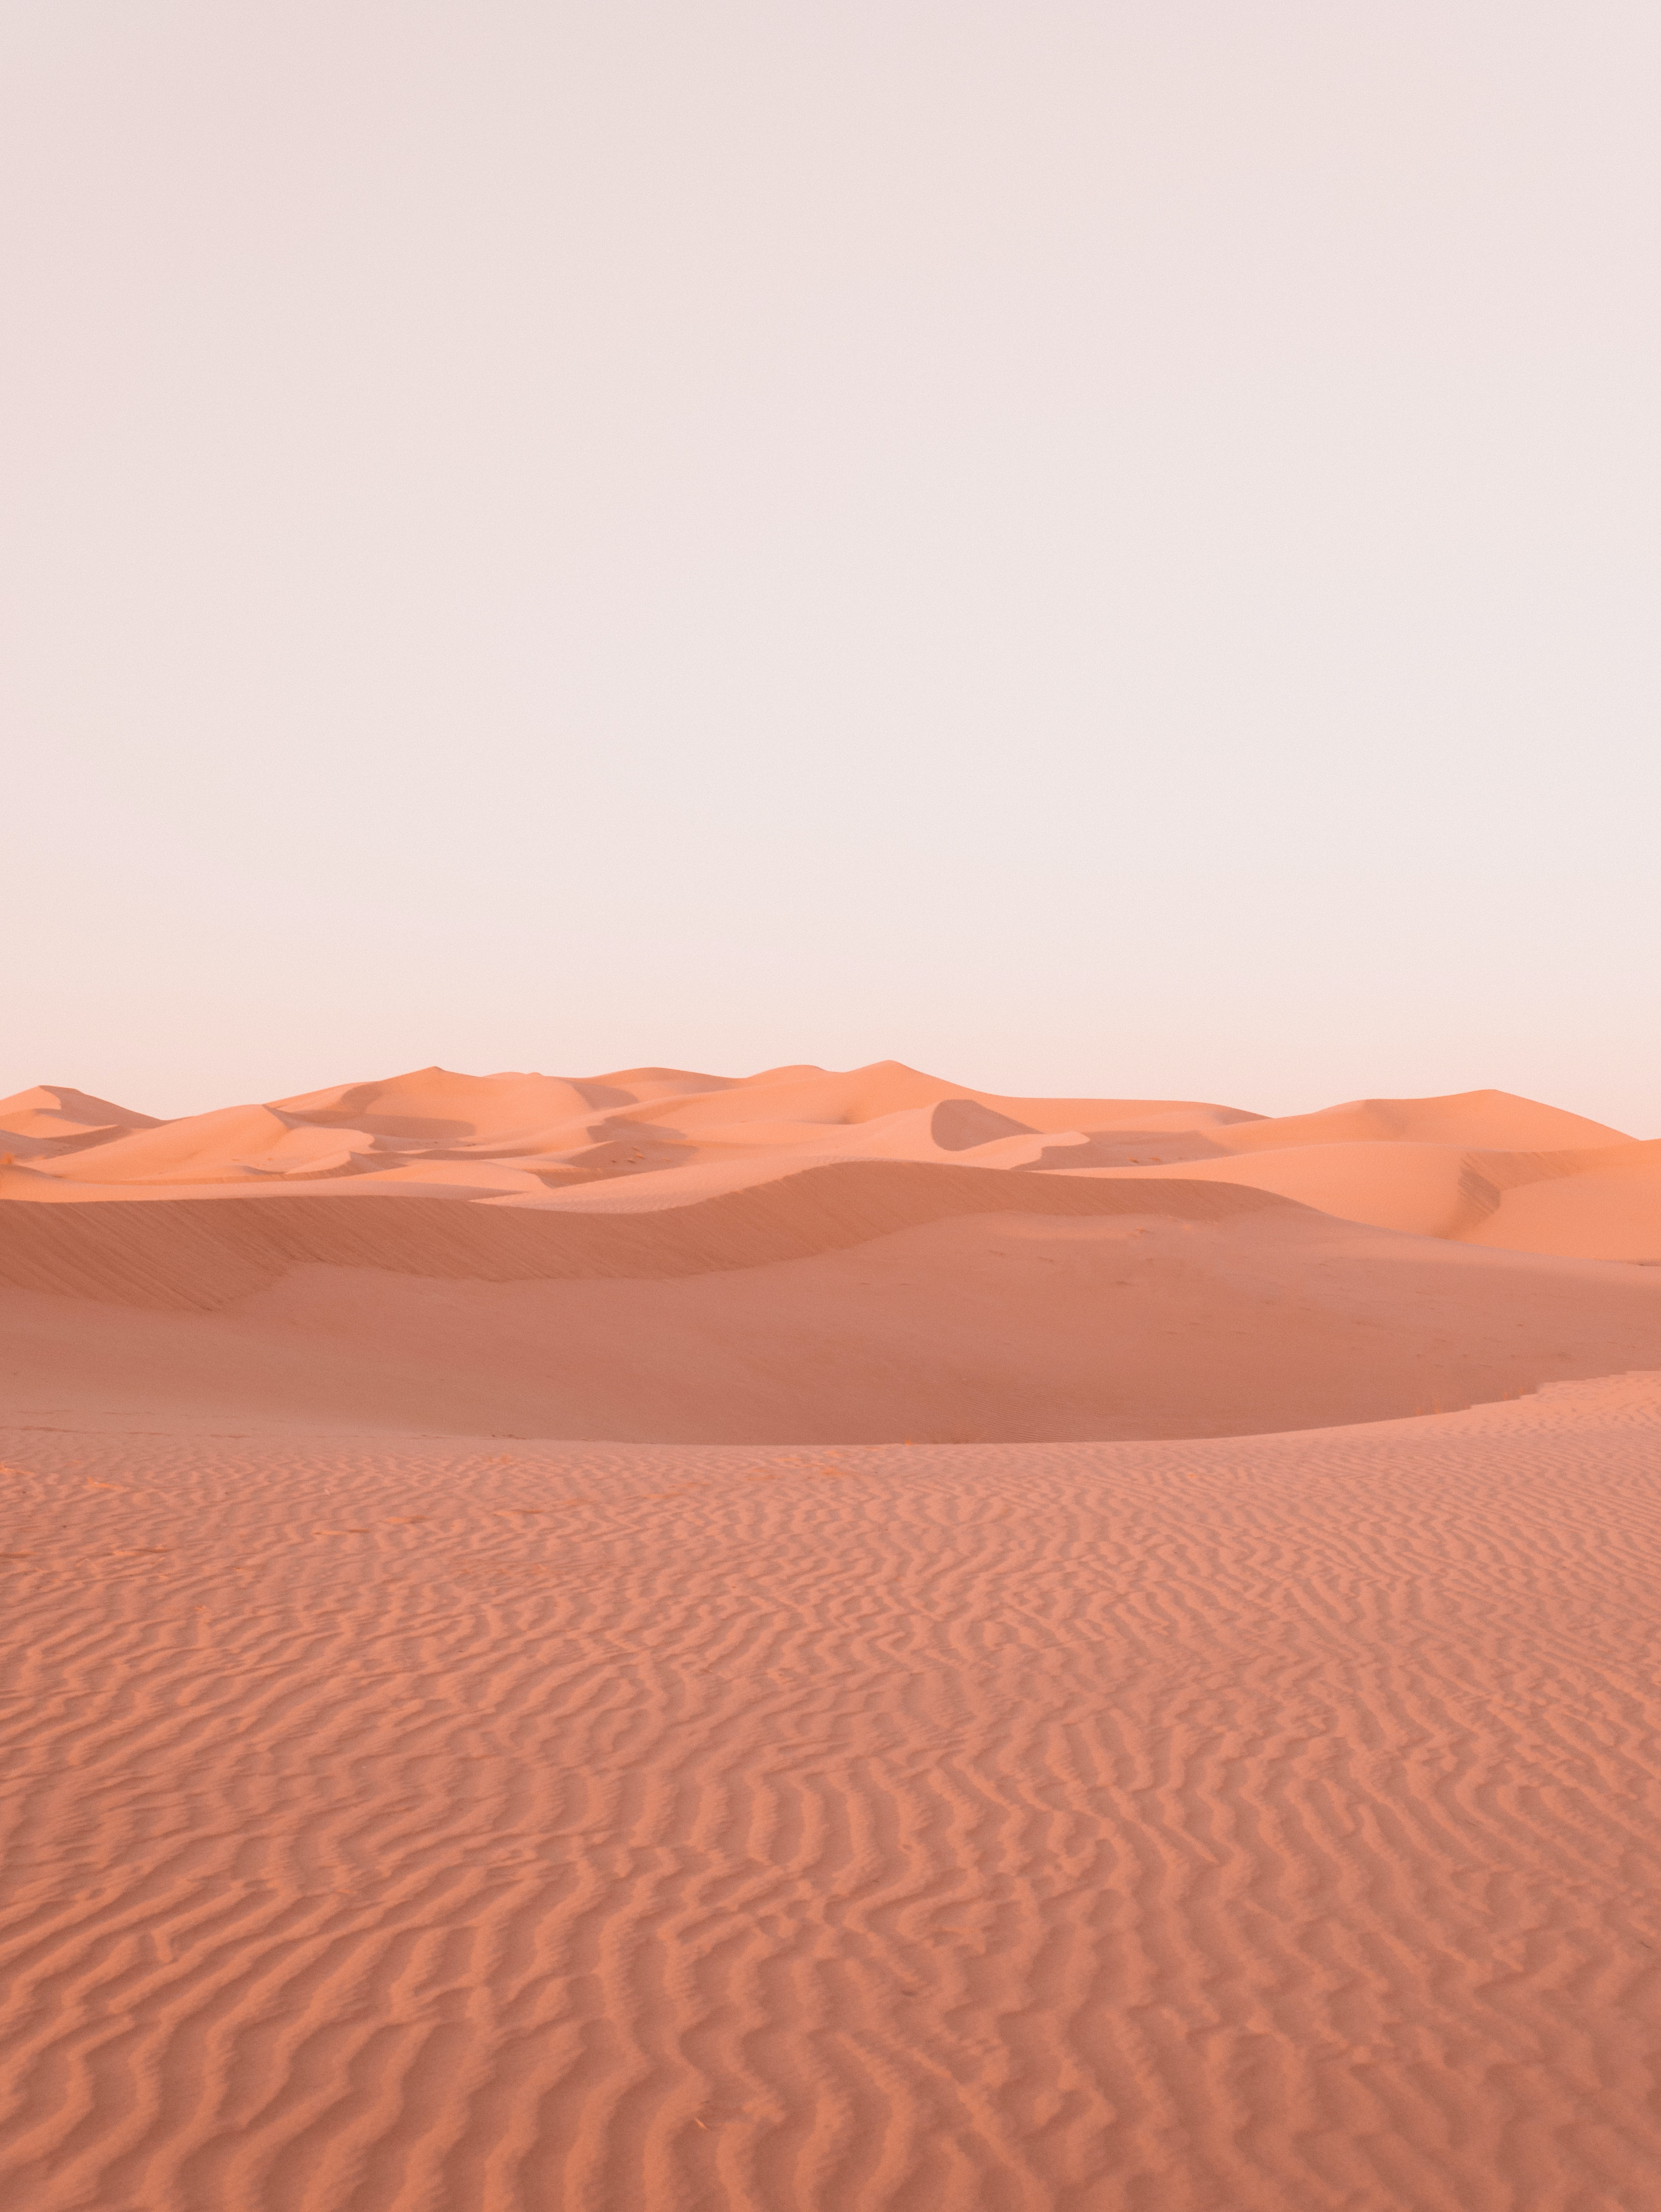
\includegraphics[height=5cm ]{imgs/streaks_dessert.jpg}
% 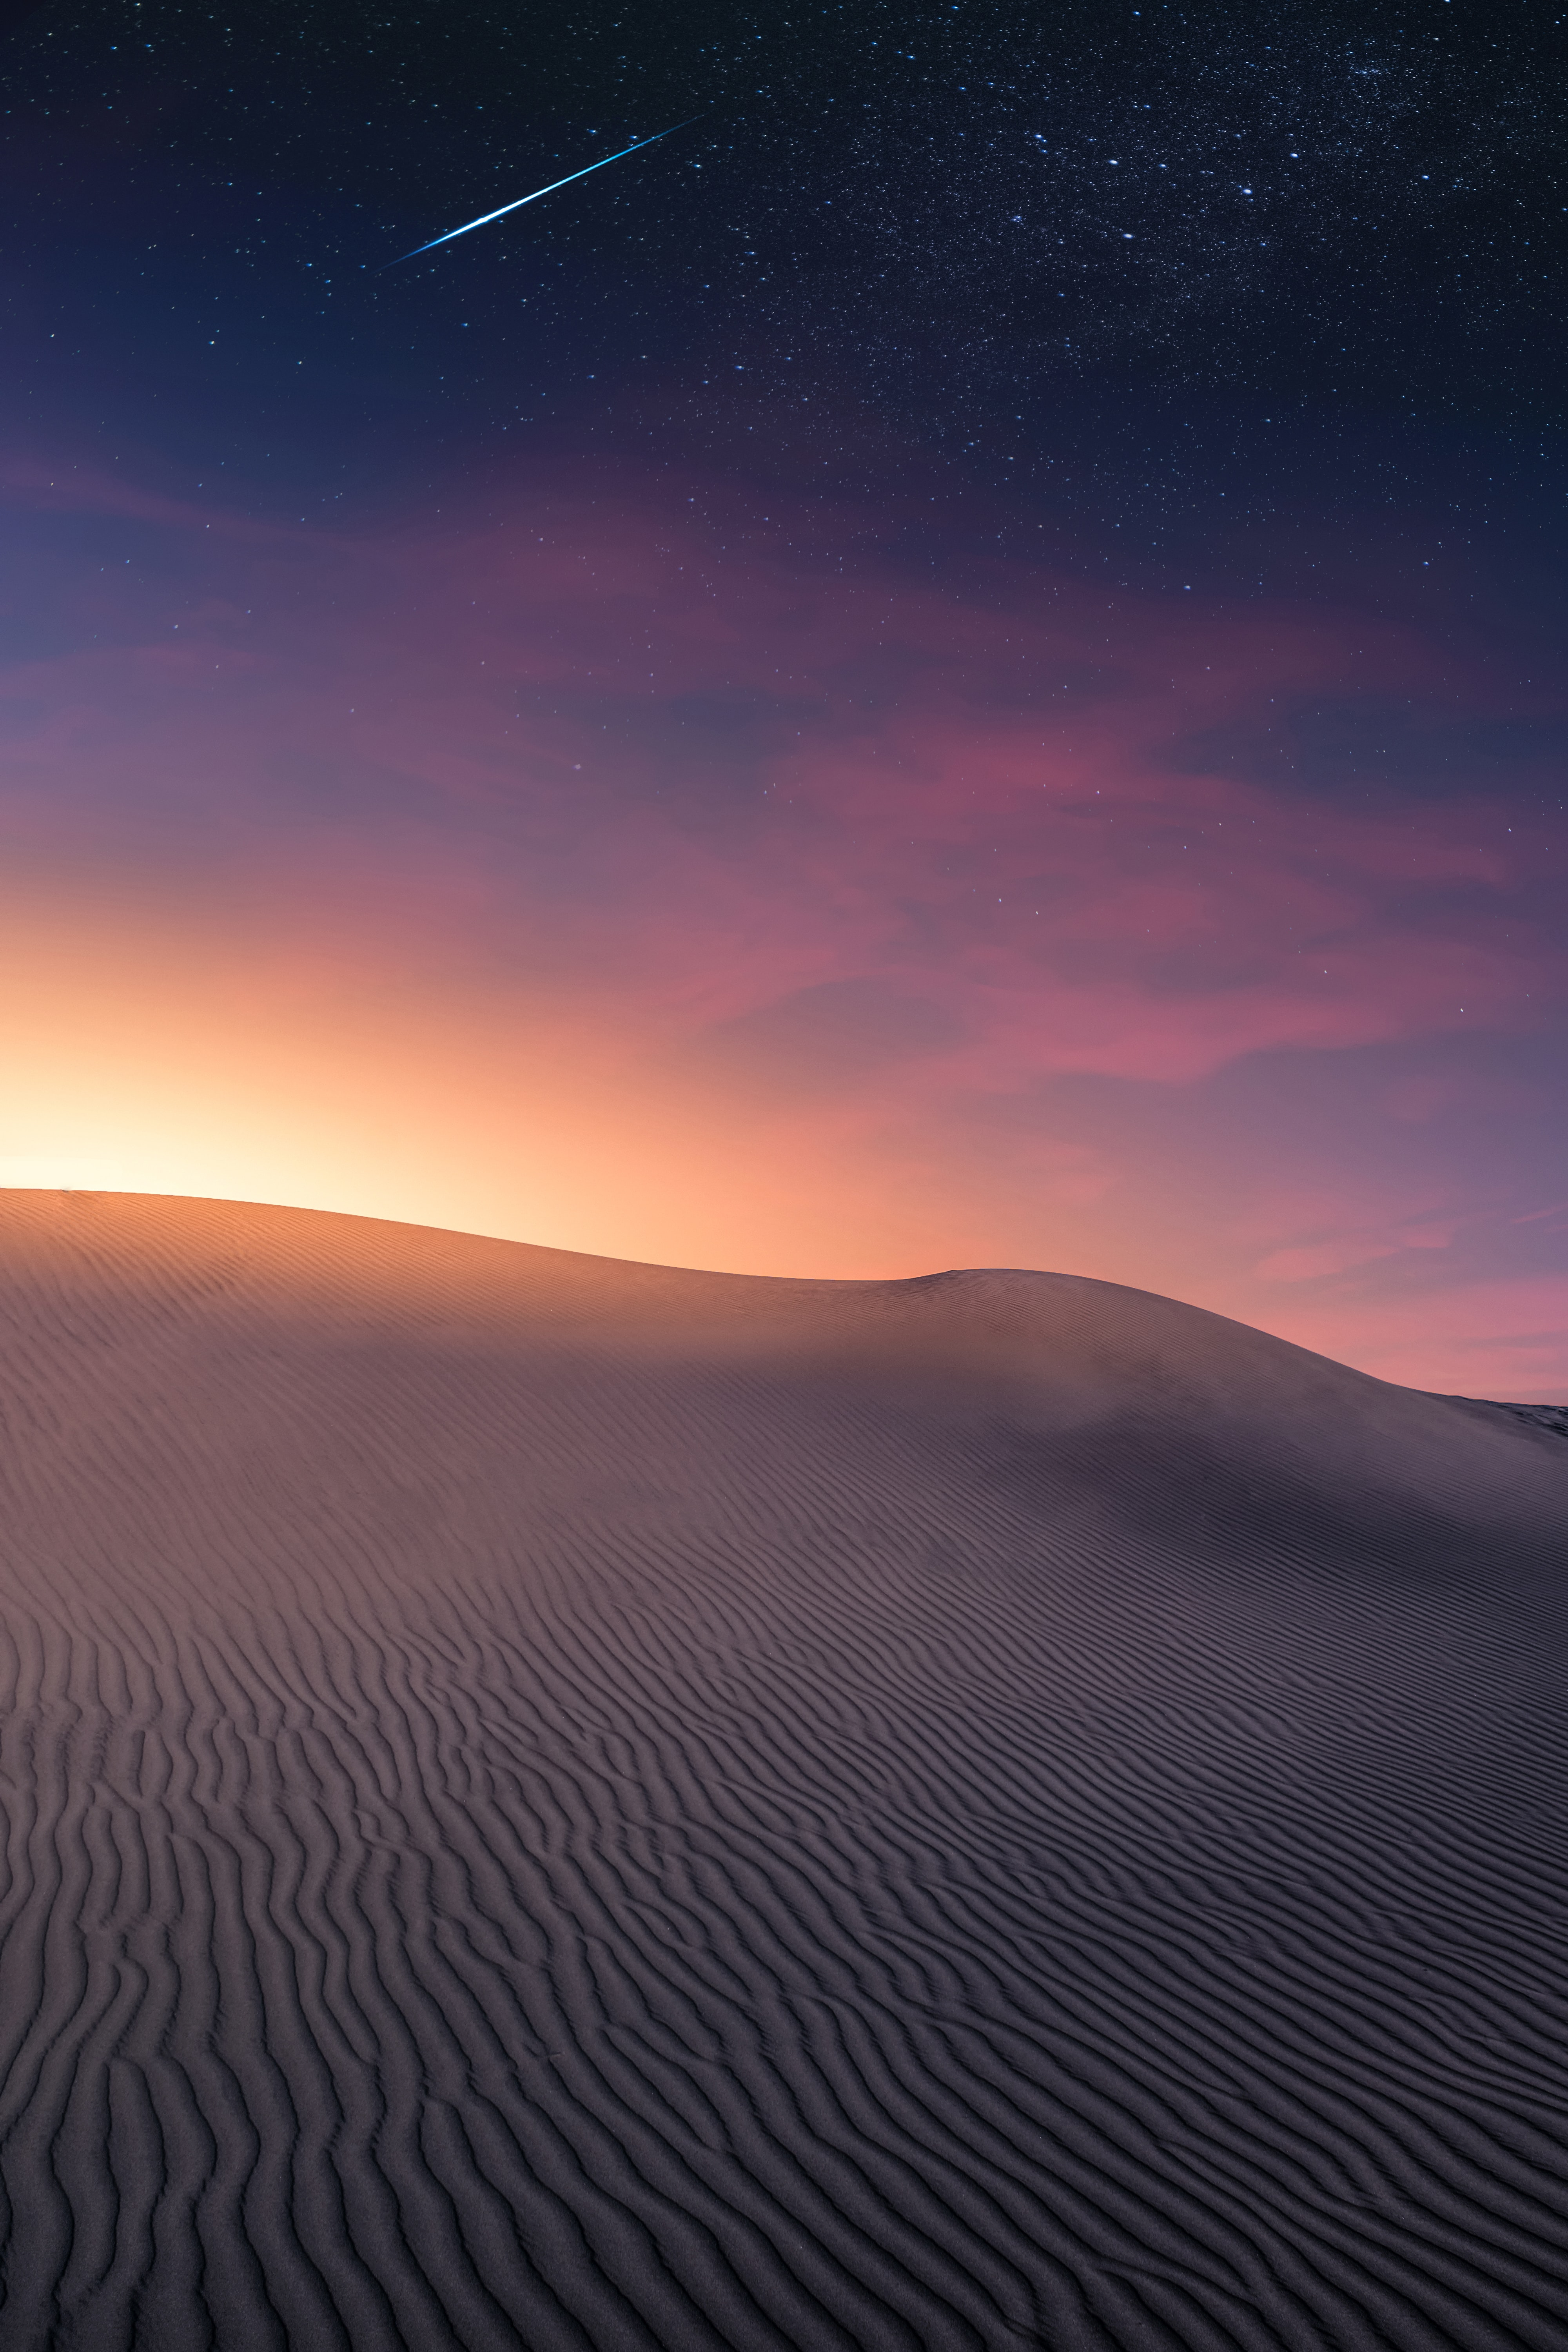
\includegraphics[height=5cm ]{imgs/streaks_dessert_2.jpg}

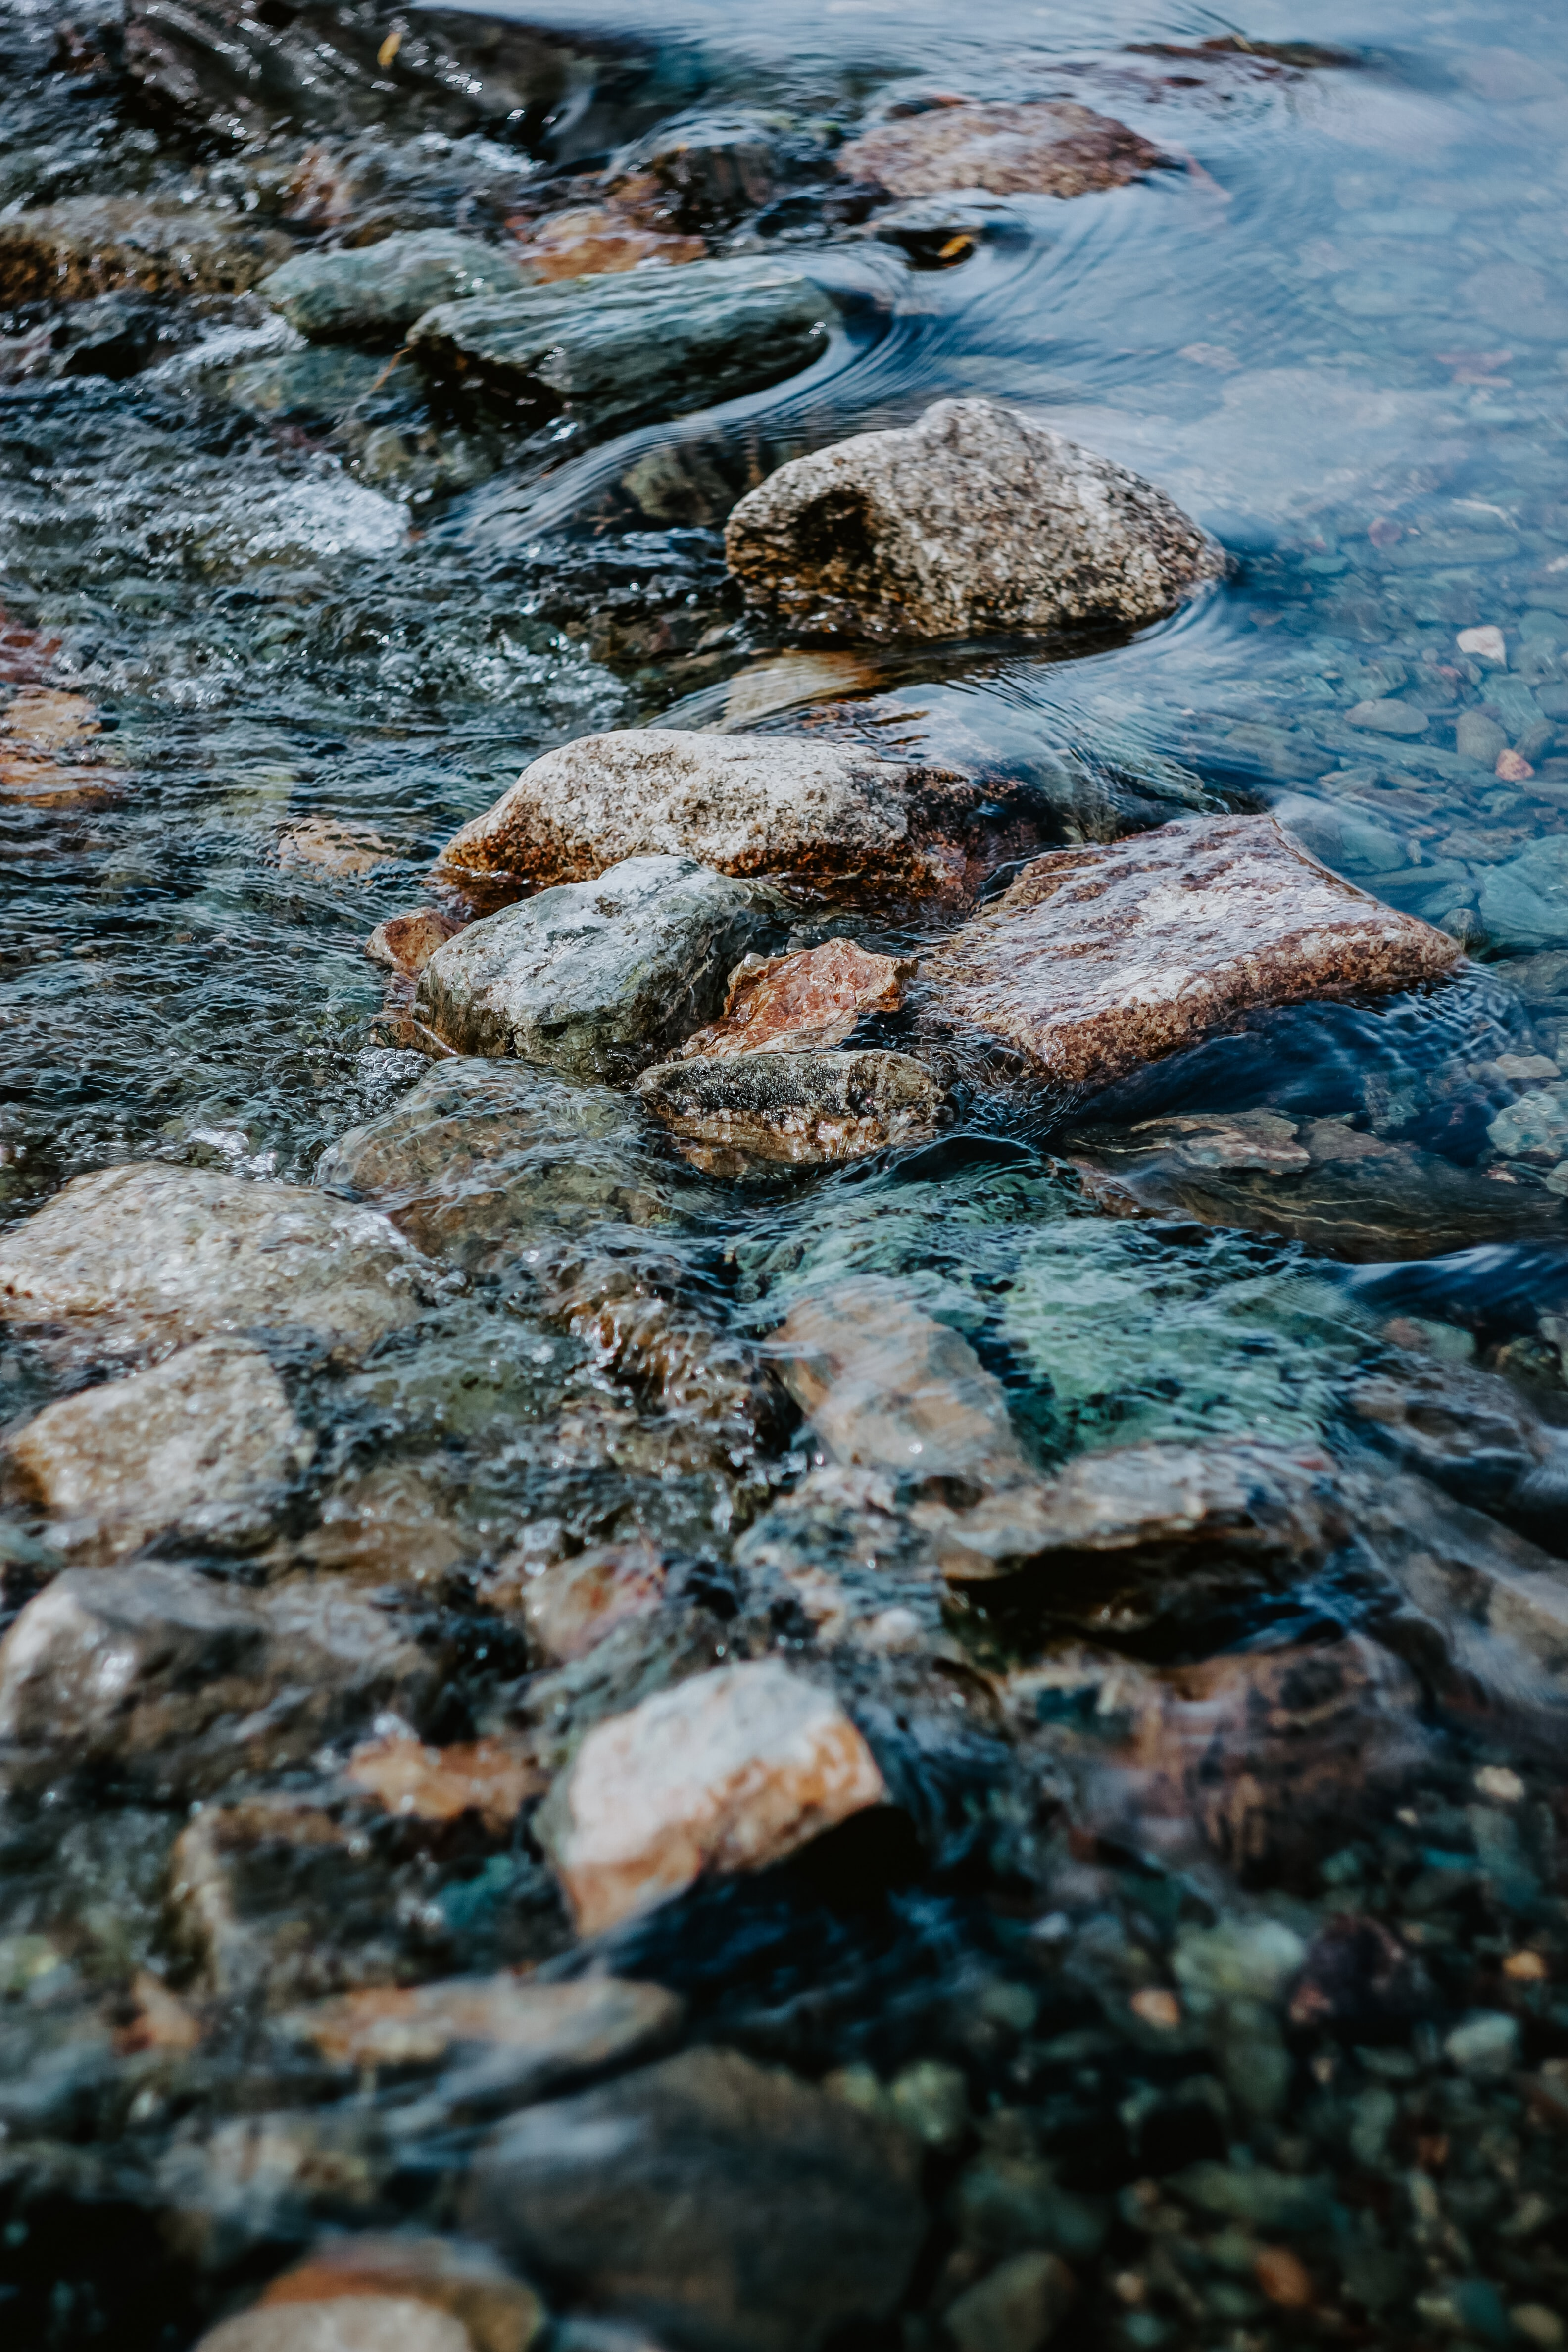
\includegraphics[width=0.24\textwidth ]{laminar_turbulent_1.jpg}
% 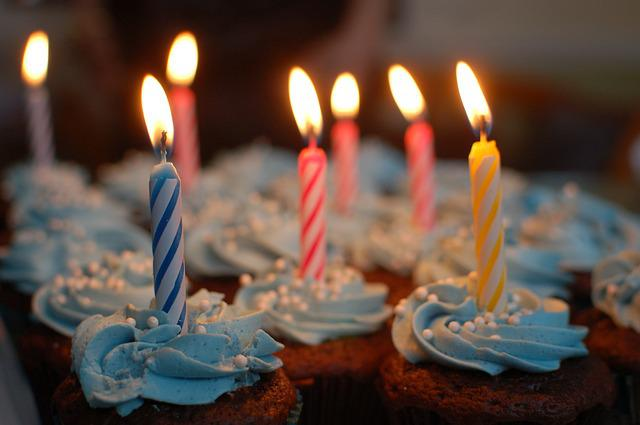
\includegraphics[width=5cm ]{llama_laminar.jpg}
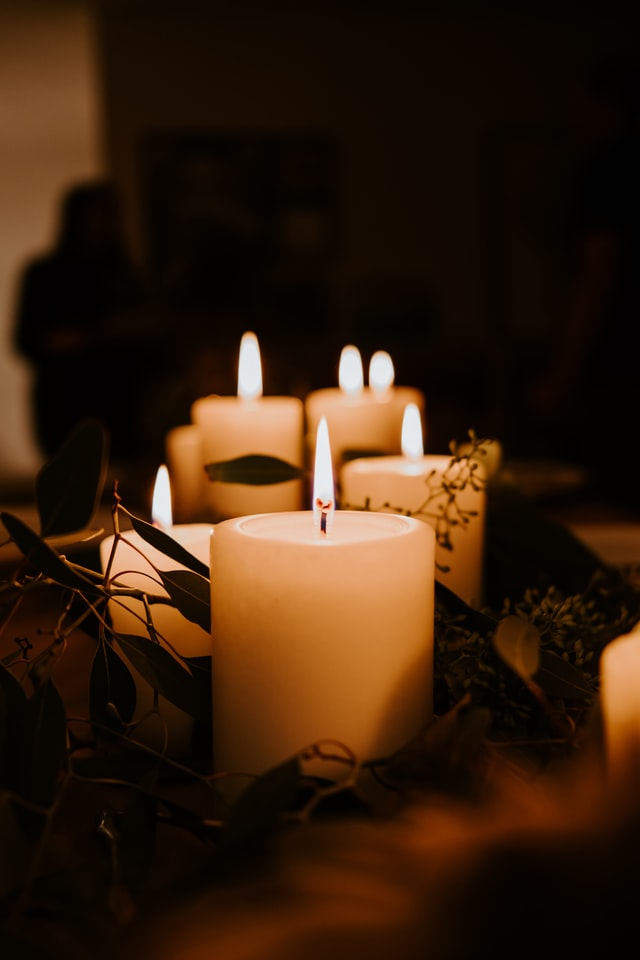
\includegraphics[width=0.24\textwidth ]{velas.jpg}
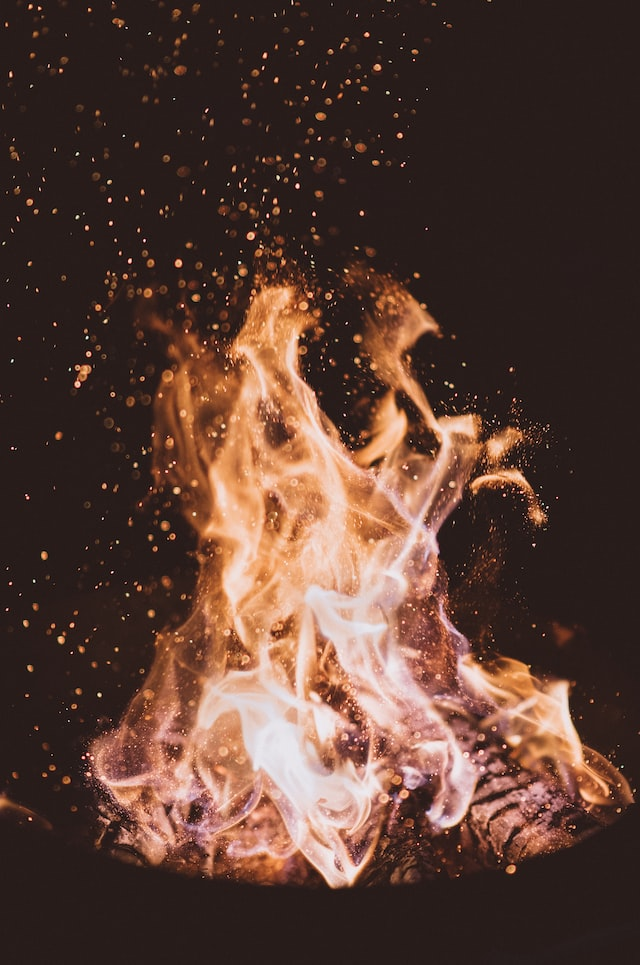
\includegraphics[width=0.24\textwidth ]{hoguera.jpg}
% 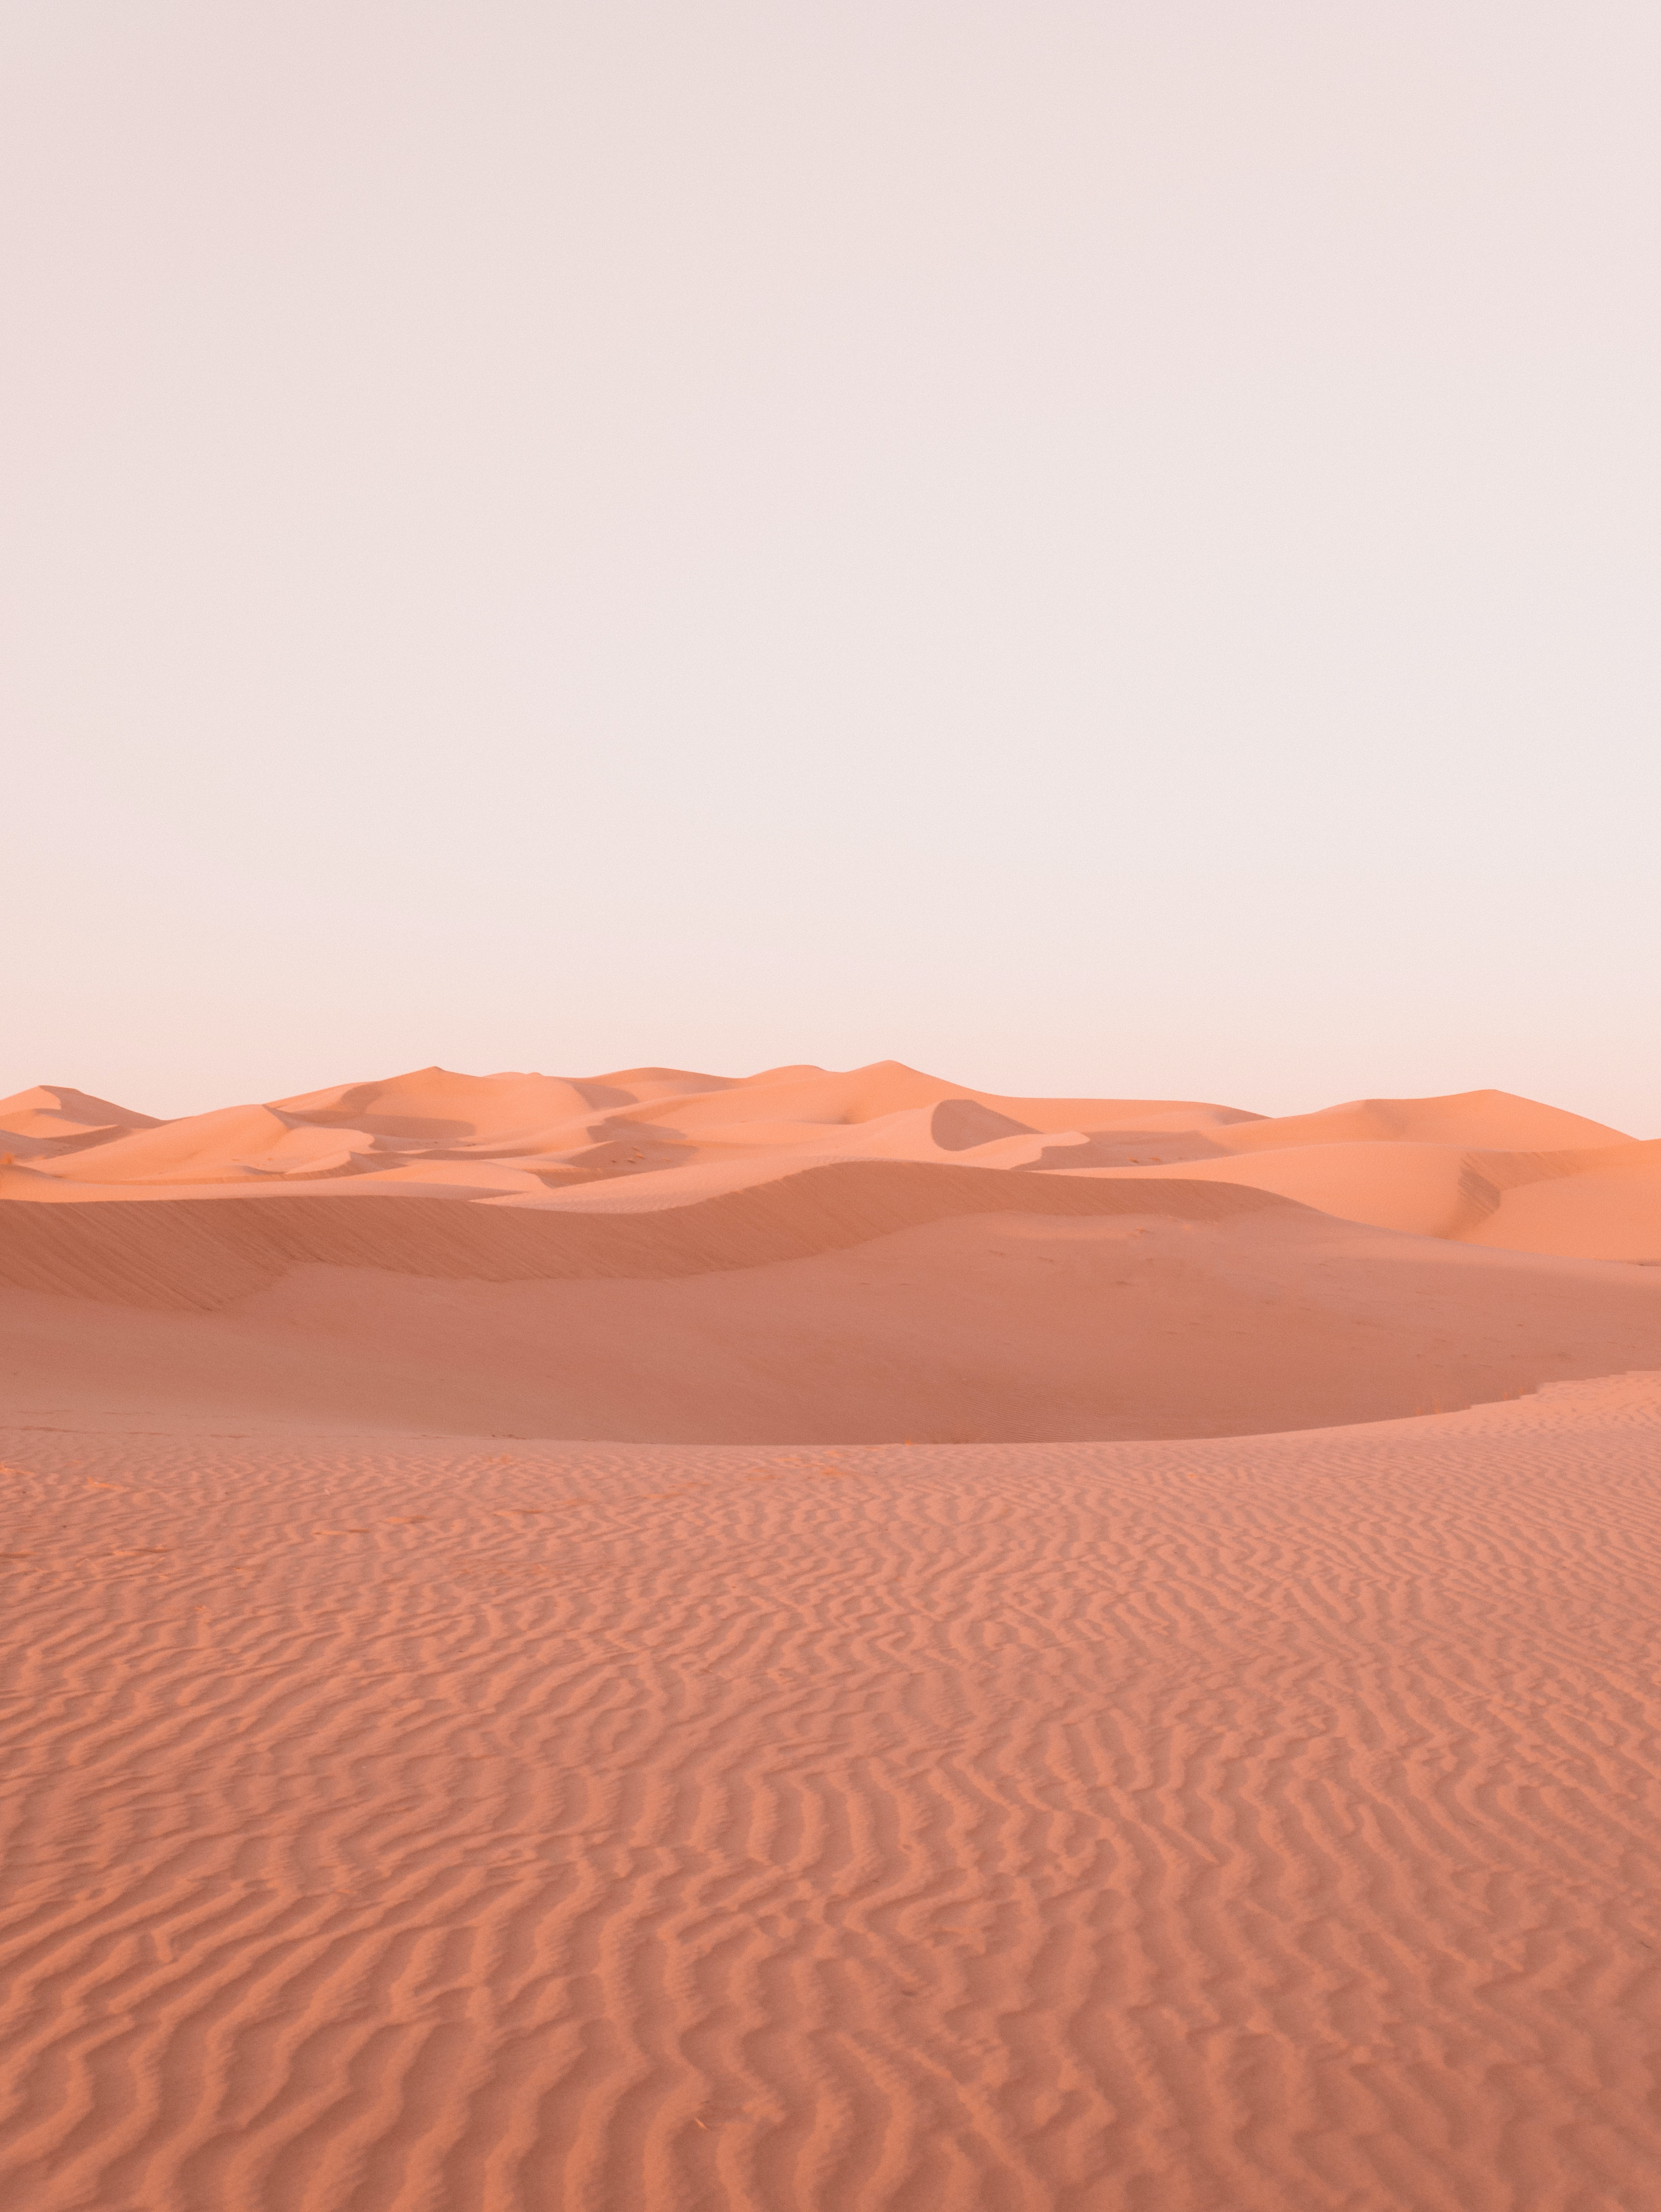
\includegraphics[width=0.2\textwidth ]{imgs/streaks_dessert.jpg}
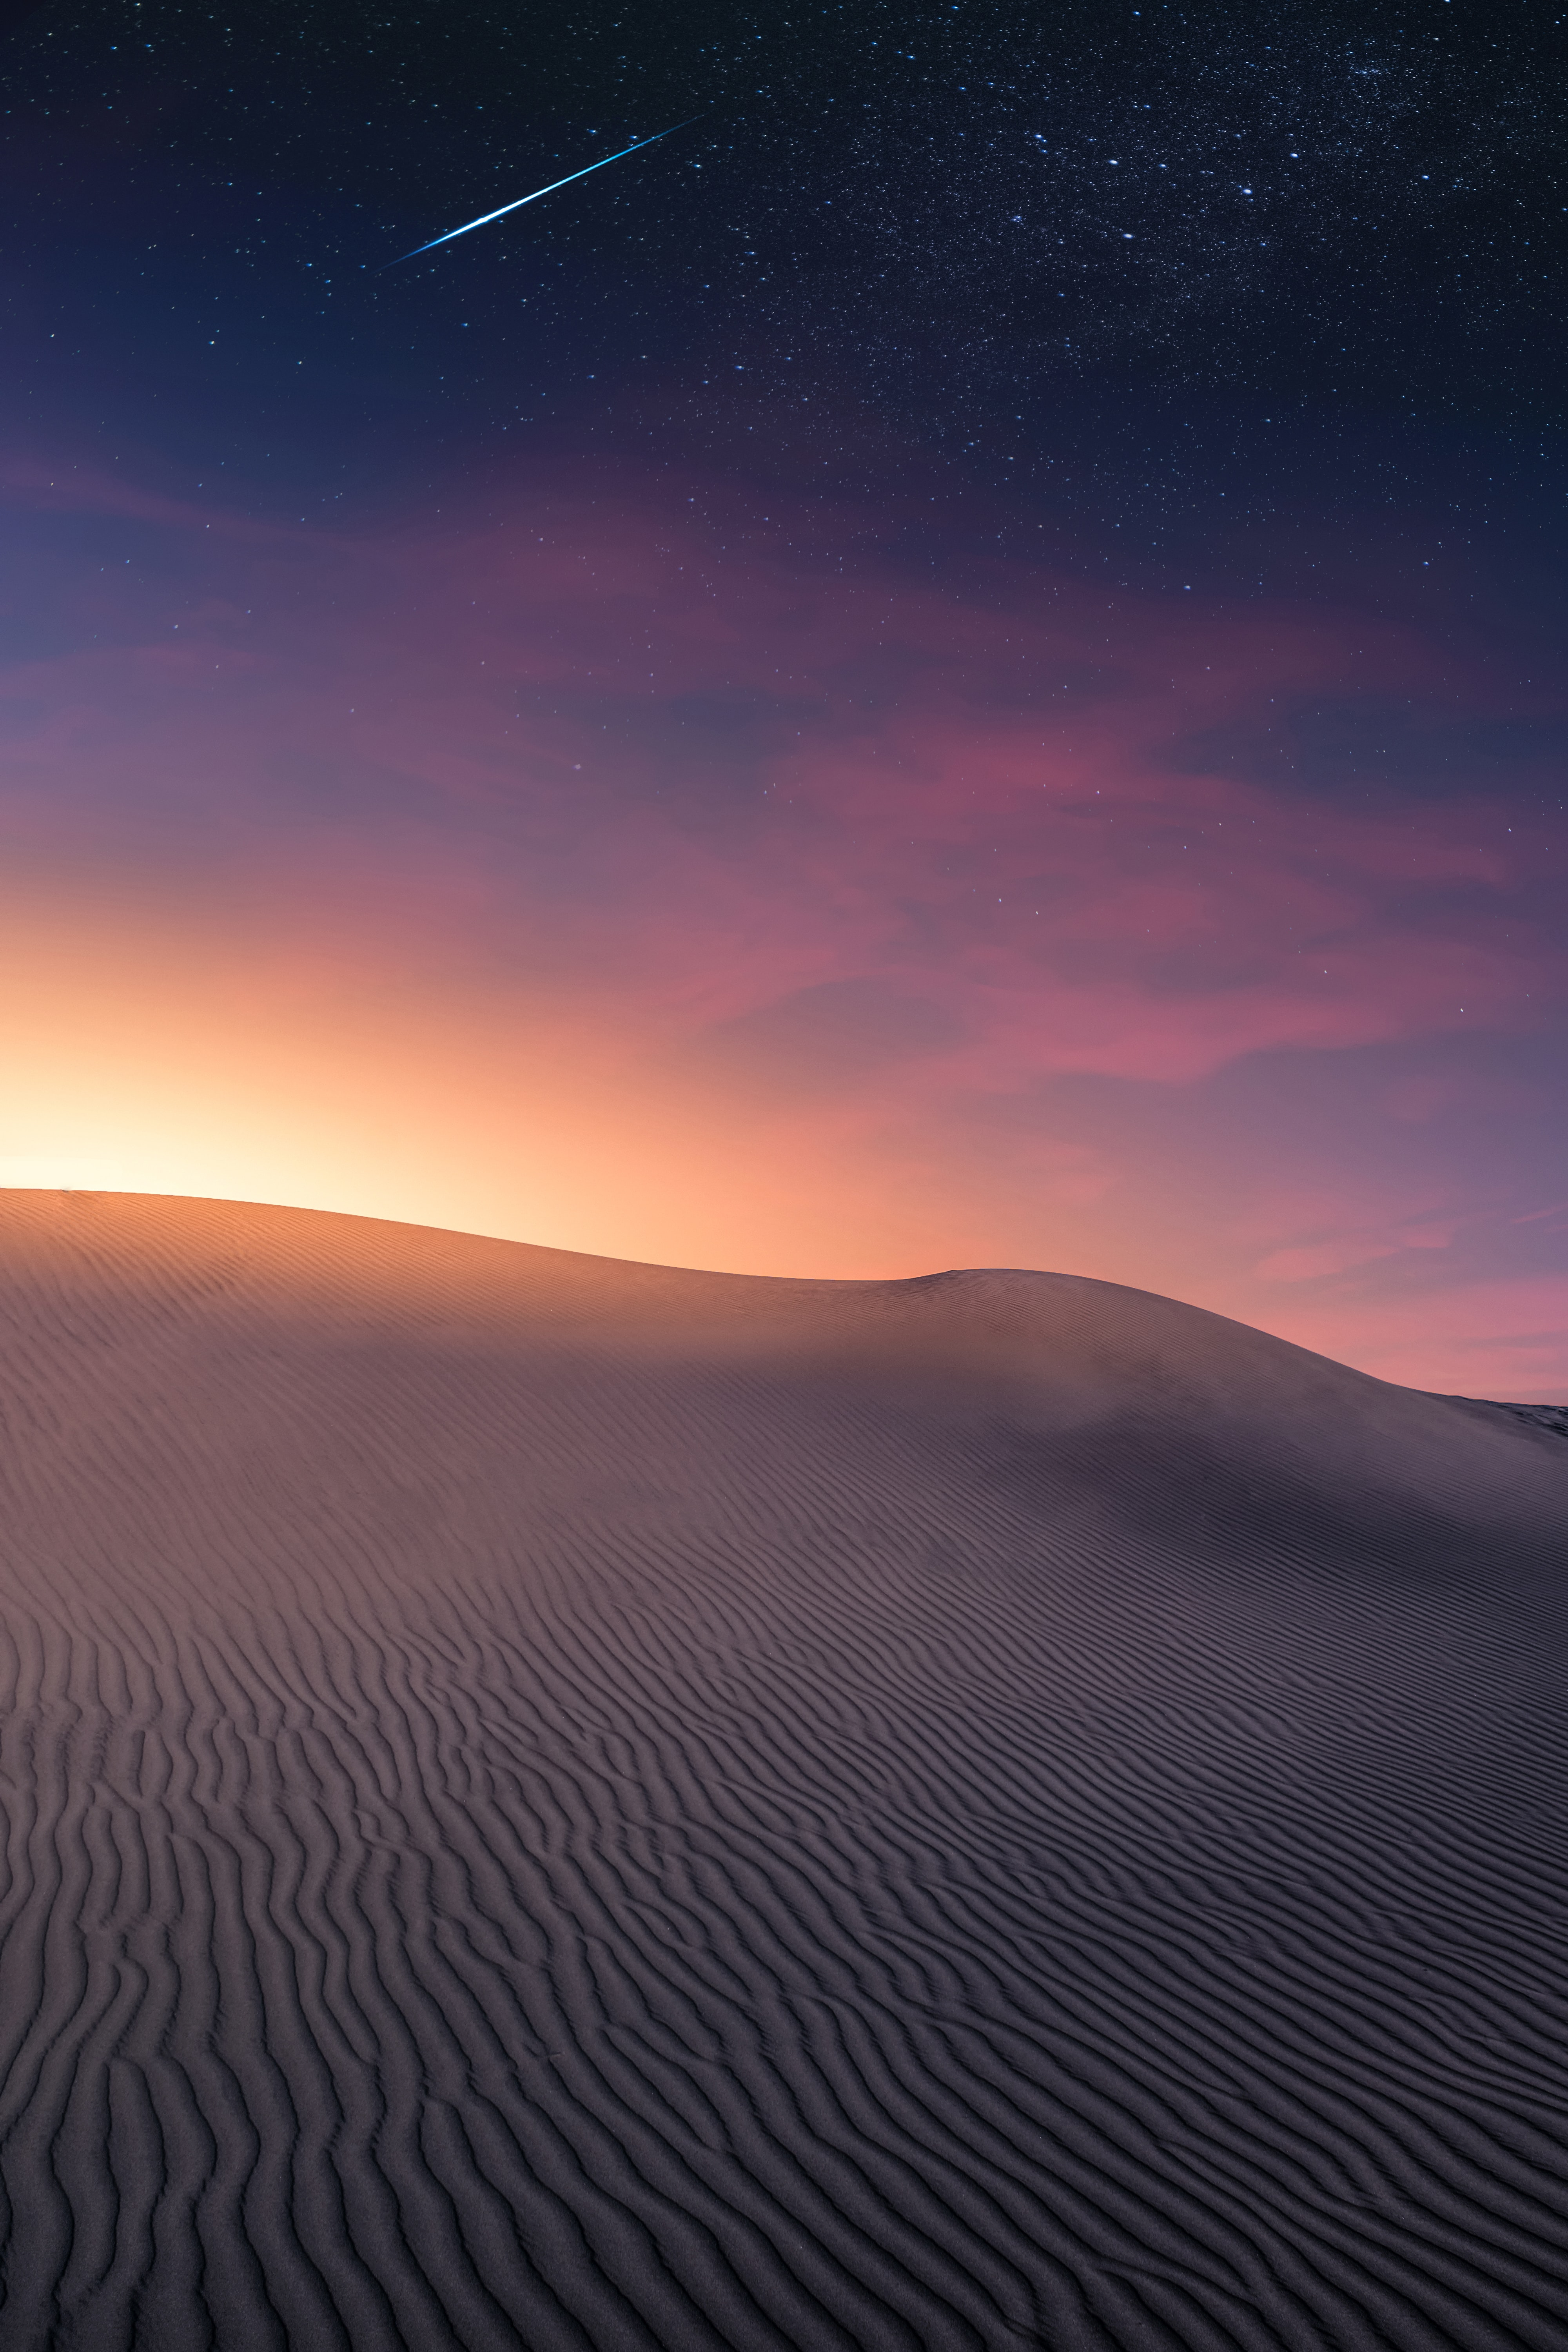
\includegraphics[width=0.24\textwidth ]{imgs/streaks_dessert_2.jpg}

\caption{ \label{fig:lam_turb} 
\highlight{
Examples of ordered laminar flow and chaotic turbulent motions in different materials. (Left) water in a shallow river, laminar on the righ side, turbulent after going through the rocks. (Mid-left) Fire in candles following an initial ordered upward motion (laminar). (Mid-right) Fire in a bonfire where the combustion gases are in a turbulent regime. (Right) Dunes in a desert flow due to the action of wind and gravity, the surface shows fine grooves as a result of the turbulent streaky structures of the wind flow over the sand surface. Figures extracted from: \url{https://unsplash.com/es/fotos/B8y6uvTnEvU} ,
\url{https://unsplash.com/es/fotos/e7cDMN6f0gs} ,
\url{https://unsplash.com/es/fotos/7qjqQjt7zXQ} and
\url{https://unsplash.com/es/fotos/MljwsnGwdOY} .   
}
}
\end{figure}

Laminar and turbulent regimes exhibit advantages and disadvantages depending on the application under consideration. 
In aerodynamic applications we usually focus in minimizing the friction present at the solid-wall boundary or maximizing the lift-to-drag ratio. coefficient. In that regard, the laminar boundary layer produces less friction than a turbulent boundary layer because 
\rev{it alters less the flow.}
\highlight{of its reduced momentum close to the wall.}
Detachment of the flow is an undesirable effect produced by strong adverse pressure gradients, and in this regard, the laminar-flow structure is more sensitive to detachment under APG conditions than a turbulent flow.

To study turbulent boundary layers (TBLs) and the effects of adverse pressure gradients (APGs) we will compare APG TBLs with a TBL subjected to zero-pressure-gradient (ZPG) conditions. A favourable pressure gradient (FPG) stabilizes and it can potentially relaminarize the boundary layer, and its effects are not critical such as those provoked by APGs, where the boundary layer can detach from the wall producing undesirable effects such as an increase in drag or even losing the aerodynamic control in airplanes.
In order to study this kind of wall-attached fluid-flow problem, first we should analyze the involved elements, such as the fluid and the solid elements.

\section{Fluid properties}

When studying the mechanics of a solid we track the positions, velocities and accelerations, forces and torques along its movement in space and time. This is the Lagrangian approach to Mechanics.
For a flow of particles or a fluid it is often more interesting to observe the flow variables at specific locations and observe the temporal change of those variables at those locations. This is the Eulerian approach that will be used to study the mechanics of a fluid flow. 

The main variables are the flow velocities, $\pmb{u}(\pmb{x},t)=u_i=(u,v,w)$, and the pressure $p(\pmb{x},t)$.
To simplify the study of adverse-pressure-gradient turbulent boundary layers the analyzed fluid is isotropic (its properties are the same in all directions) and Newtonian, which implies that the viscous forces are a linear function of the strain-rate tensor $s_{ij}=\pdv{u_i}/{x_j}$. As an example, the friction at the wall is $\tau_w=\mu \pdv{u}/{y}$,
where $\mu$ is a constant factor: the dynamic viscosity.
The density and viscosity of the fluid combines into the kinematic viscosity $\nu=\mu/\rho$ with units $[m^2/s]$. 
Note that we consider the density and viscosity as constant and not affected by changes in temperature.
\rev{, the temperature of the fluid is not relevant and the energy and momentum evolution are decoupled.}

\section{Solid properties}
In general, the solid boundaries are curved, specially in aerodynamic applications where the curvature is used to create differences in pressure that lead to forces in the desired directions. The forces in the direction of the inflow are called drag and the forces in the perpendicular direction is called lift. For curved boundaries, different coordinate systems are used. The local system of coordinates that changes with the solid boundary is where the surface forces are calculated. The surface forces are then projected onto the global coordinates associated with the inflow to obtain the lift and drag.
For flat plates with zero angle of attack the global and local coordinates are the same.
The surface of the flat plate that we study is rigid and smooth, and no exchange of heat or mass is produced between the fluid and the solid. In the interface fluid/solid the only interaction is due to pressure and viscous forces that adapt the fluid velocity to the solid surface velocity.
The flat plate will be considered to be static in the global system of coordinates.


\section{Boundary layers}

Boundary layers are regions inside a fluid flow where certain features or changes in the properties of the fluid are concentrated. Historically the first idea of boundary layer is set for the adaptation region of the fluid momentum from outer conditions to the conditions in a solid surface.
Other boundary layers are for example thermal boundary layers where the focus is on the change of thermal properties.

When we consider the flow around a solid object in incompressible conditions, the flow can detect the presence of the solid object and adapt its trajectory. The flow then surrounds the solid starting from the leading edge and close to the solid surface the boundary layer is the region where the velocity of the flow adapts from the solid surface velocity to the outer-flow velocity. The boundary-layer thickness has to be defined according to the main idea of a region of the fluid close to the solid wall that encloses the major viscous effects created due to the fluid/surface interaction. An obvious effect of the presence of a wall is that the streamwise velocity has to adapt from the velocity of the solid boundary to the exterior velocity, commonly called velocity at the infinity or freestream velocity $U_{\infty}$. 
In general, for a certain streamwise location, the velocity is measured in the wall-normal direction, obtaining a profile of instantaneous streamwise velocity $u(y,t)$. Then $U_{\infty}=U(y\rightarrow \infty)$ (where capital letter denotes mean velocity) is the unperturbed velocity and can change from one streamwise position to another.
In the case of zero-pressure gradient boundary layers, $U_{\infty}$ is taken as constant, since in a steady flow in the absence of viscous forces, $\pdv{U}/{x}$ should be zero. 

Since an obvious property of the boundary layer is the adaptation of the streamwise velocity, the boundary layer can be defined using this property and the $99\%$ thickness $\delta_{99}$ is defined as the wall-normal position where $U(y=\delta_{99})~=~0.99U_{\infty}$.
In Fig.~\ref{fig:lam_turb_profiles} we show an example of how the mean streamwise velocity $U(y)$ adapts from the velocity at the wall $U(y=0)=0$, to the outer velocity $U_{\infty}$ on laminar and ZPG TBL profiles.

\begin{figure}[h!]
\centering
% \captionsetup{width=0.99 \textwidth}
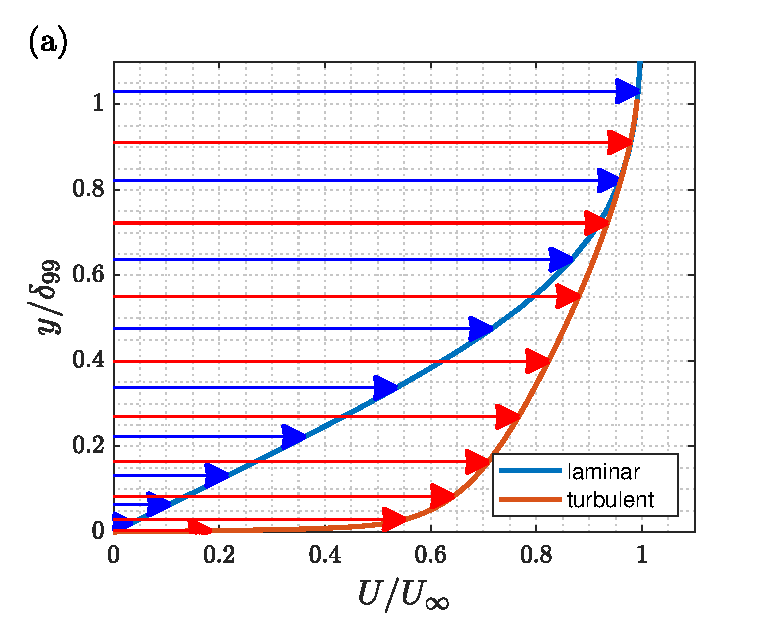
\includegraphics[width=0.6\textwidth]{imgs/lam_turb/ZPG_lam_turb.eps}
\caption{ \label{fig:lam_turb_profiles} Mean streamwise velocity profile of a laminar and a turbulent boundary layer subjected to a ZPG.
   }
\end{figure}

In the case of curved boundaries, the curvature induces a pressure gradient since the incoming flow has to adapt to the curvature of the wall. On a flat plate, a pressure gradient can be produced by controlling the exterior flow, usually the streamwise gradient of the streamwise velocity $\pdv{U_{\infty}}/{x}$


\subsection{Turbulent boundary layers}
The characteristics of a boundary layer change radically depending on the laminar/turbulent regime.
In a laminar boundary layer, any perturbation produces shear stresses and therefore, viscous forces, which are transported by the momentum of the flow and eventually dissipated by the viscous dissipation. 
Highly-energetic perturbations, flow configurations or certain viscosity/momentum forces ratios are unstable, implying a change of regime, usually from the laminar regime to turbulence. 
The ratio between inertial and viscous forces is called Reynolds number $\Rey=U_{sc} L_{sc} / \nu$, and depending on the chosen velocity and length scales $U_{sc}$ and $L_{sc}$ we would be analyzing different phenomena. The Reynolds number where a flow configuration changes regime is called critical Reynolds number $\Rey_c$.
Note that if $U_{sc}=U_{\infty}$ and $L_{sc}=c$ where $c$ is the chord of a wing profile, then we are setting the global configuration of the problem. If we want to analyze a local phenomenon such as the different size of the flow scales close to the wall compared to the largest ones, we can use the Reynolds number based on the friction velocity $\Rey_{\tau}=u_{\tau}\delta_{99}/\nu$, where  $u_{\tau}=\sqrt{\tau_w / \rho}$.

In the turbulent regime, the momentum and energy of the flow initiate a cascading effect breaking the initial ordered motions into chaotic submotions. 
Eddies are generated, and they extract energy from the mean flow, then dividing into smaller eddies (note that there is also an inverse cascade of energy transfer from smaller to larger scales). Then a transport of energy between large and small eddies is produced. Eddies are regions with strong shear stresses, therefore the viscous forces are stronger and produce a dissipation of the kinetic energy.
The boundary layers studied here are momentum boundary layers that confine the turbulent perturbations and mayor viscous effects produced because of the presence of a solid boundary.

\rev{In a turbulent boundary layer, the thickness of the boundary layer should delimit the region of the flow close to the wall that exhibit the turbulent fluctuations and viscous forces produced by the presence of a solid boundary,} leading to different definitions for the boundary-layer thickness.
For laminar BLs and ZPG TBLs, the previously-defined $\delta_{99}$ thickness, where the mean velocity of the flow is $99\%$ of the exterior velocity, is valid and is based only on the adaptation of the mean streamwise velocity to that of the outer flow.
For other TBLs with pressure gradients, the outer velocity can have gradients in the streamwise and wall-normal directions. In the case of TBLs subjected to streamwise pressure gradients we can use an approach based on the level of turbulence such as the one used in \cite{diagnostic_Vinuesa} where the boundary-layer thickness is such that it captures the turbulence up to certain turbulent level.
This approach is useful for the dataset that we use, since the turbulent levels outside the TBL are minimal, both in the simulations \citep{EAmorZPG, bobke2017, Pozuelo_JFM_22}, and in the experimental databases \citep{Sanmiguel_PRF}.
If the freestream turbulent level is high, the method in \cite{diagnostic_Vinuesa} is not applicable. 
Other methods have been proposed in the literature and a review was given by \cite{d99_determination_2020}.

Turbulence exhibits a wide range of motions, and one way to study and characterize turbulence is through decomposition of those characteristics. 
The first approach is an statistical characterization where we can divide the flow variables into a mean or average value and a perturbation; this is known as the Reynolds decomposition \citep{Rey_decomp}.
The fluctuating character of the flow is shown for a flat-plate TBL in Fig.~\ref{fig:lam_turb_development} where we show contour levels in snapshots of the instantaneous streamwise velocity. \highlight{In Fig.~\ref{fig:lam_turb_development}(a) we show the initial laminar ZPG flow-field used to initialize the APG simulation. The contours are smooth and show a well-defined laminar behaviour with small perturbations introduced to trigger turbulence. The red line is the position where $u=0.99U_{\infty}$. In Fig.~\ref{fig:lam_turb_development}(b) the turbulence is totally developed and correspond to the APG simulation when the final APG conditions are reached. The red line correspond to $U=U_e$ which is the outer velocity or ``edge velocity'' calculated through the method in \cite{diagnostic_Vinuesa}. It is possible to see how at different streamwise positions $x/\delta^*_0$ (where $\delta^*_0$ is the inflow displacement thickness) the instantaneous velocities close to the red line are decreasing, this is due to the APG boundary condition, where $U_e$ decrease along $x$ to produce a near-equilibrium APG. The edge velocity depends on the method used to determine the boundary-layer thickness.
}
\begin{figure}[h!]
\centering
% \captionsetup{width=0.99 \textwidth}
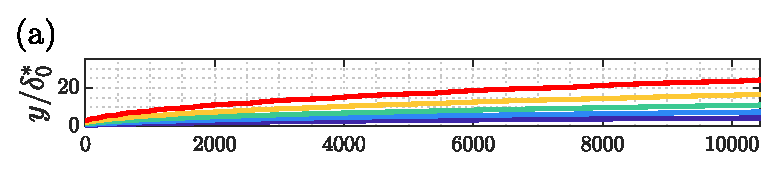
\includegraphics[width=0.99\textwidth ]{imgs/lam_turb/APG_laminar_test.eps}\\
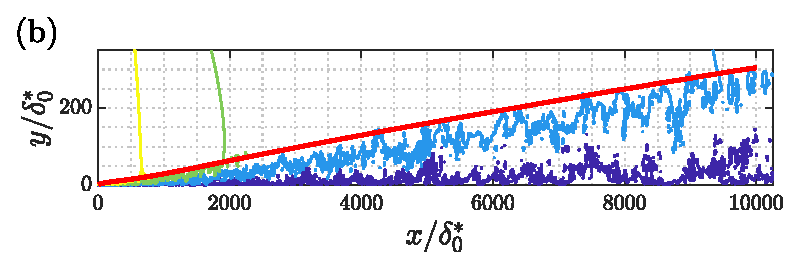
\includegraphics[width=0.99\textwidth ]{imgs/lam_turb/APG_turb_test.eps}
% 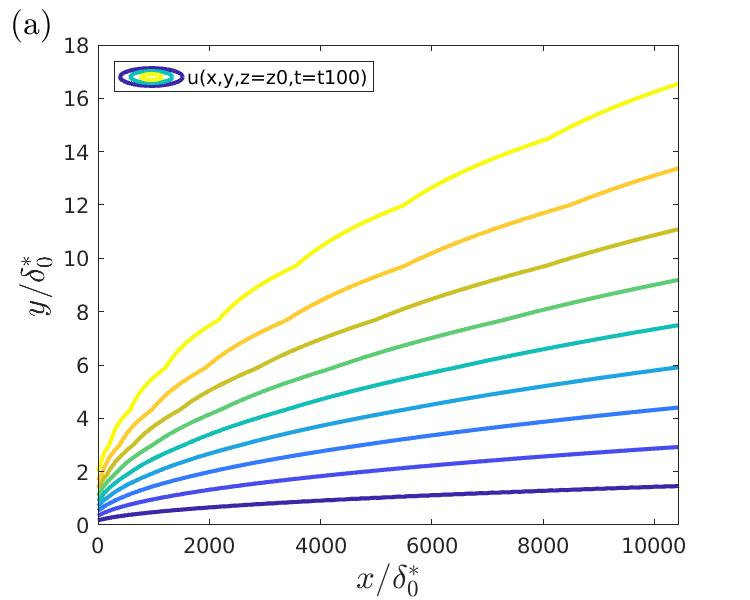
\includegraphics[width=0.49\textwidth ]{APG_laminar.jpg}
% 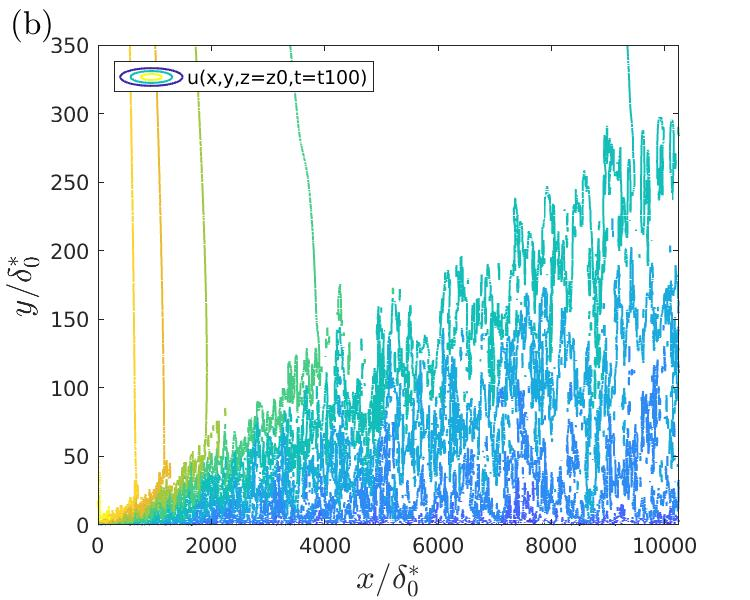
\includegraphics[width=0.49\textwidth]{APG_turb.jpg}
\caption{ \label{fig:lam_turb_development} Snapshot of the instantaneous streamwise velocity $u(\pmb{x})$ in 
\highlight{
(a) initial ZPG laminar flow-field used for the APG simulation and (b) turbulent APG boundary layer.
The contours are taken at $u=0.3, 0.5, 0.7, 0.9 U_0$, where $U_0=U_{\infty}(x=0)$ is a reference velocity.
The red line shows the thickness of the BL, $\delta_{99}$ where $u(y=\delta_{99})=0.99 U_{\infty}$ for the ZPG laminar case (a) and for the APG TBL in (b) the diagnostic plot method \cite{diagnostic_Vinuesa} is used. 
}   
}
\end{figure}



\section{Mathemathical analysis}

For an incompressible flow the conservation of mass in a control volume becomes the differential continuity equation:

% Continuity
\begin{equation}
\label{eq:continuity_cap2}
% \overrightarrow{u}
    \nabla \cdot \pmb{u} = \partial_i u_i = 
    \frac{\partial u}{\partial x} + \frac{\partial v}{\partial y} + \frac{\partial w}{\partial z} = 0,
\end{equation}
which is shown as the divergence of the velocity vector, in the diadic and components notations.
To describe the time evolution of the flow variables, it is possible to use the partial differential equations in Eq.~(\ref{eq:NS_cap2}), which are are the Navier--Stokes (NS) equations, and they describe the evolution of the momentum of the flow as a function of the pressure gradient and viscous forces acting on it. The system of equations comprising Eqs.~(\ref{eq:continuity_cap2}) and (\ref{eq:NS_cap2}) is valid for both laminar and turbulent-flow regimes, depending on the configuration of the problem.

% NS Total velocities
\begin{equation}
    \label{eq:NS_cap2}
    \frac {\partial u_i} {\partial t}  + u_j \frac {\partial u_i} {\partial x_j} =
    -\frac {1} {\rho} \frac {\partial p} {\partial x_i} +  \nu \frac {\partial^2 u_i} {\partial x_j^2}.
\end{equation}

By providing boundary conditions (BCs) together with an initial state of the system and the flow properties, we can expect either laminar, transitional or turbulent flow.
Once turbulence is developed, the statistical approach to turbulence is based on the Reynolds decomposition \citep{Rey_decomp}, given in Eq.~(\ref{eq:Rey_decomp}). This decomposition is based on a constant or averaged component and a fluctuating component in a way that once they are introduced into Eqs.~(\ref{eq:continuity_cap2}) and (\ref{eq:NS_cap2}) some of the terms are simplified. An example is to use a constant base flow (such as the laminar state) plus a fluctuating flow field, which is the case used to study transition and stability of BLs. 
For our case, the mean flow $U_i$ is an average in time and the homogeneous directions. The average in a dimension $d$ is marked as $\langle . \rangle_d$, and the average in time and all the homogeneous dimensions is marked with $\overline{(.)}$. In a spatially-developing boundary layer the mean velocity is $U_i = \overline{u_i} =\langle \langle u_i \rangle_z \rangle_t$ and as a result of Eq.~(\ref{eq:Rey_decomp}), $\overline{u_i\myprime}=0$. 
% Note that $\langle u_i\myprime \rangle_z (t) \neq 0$ and $\langle u_i\myprime \rangle_t(z) \neq 0$. 

Introducing the flow decomposition Eq.~(\ref{eq:Rey_decomp}) into the continuity and NS equations (\ref{eq:continuity_cap2}) $\&$ (\ref{eq:NS_cap2}), and using the average in time and $z$, we see that the continuity equation is fulfilled for both the mean and the fluctuating component separately, see Eq.~(\ref{eq:cont_decomp}). And in the momentum equations we obtain the Reynolds-averaged Navier--Stokes equation (RANS) in Eq.~(\ref{eq:RANS_cap2}) and the equation for the time evolution of the perturbations Eq.~(\ref{eq:pertub_cap2}) as a result of substracting the RANS equations from the general NS equations.

% R Decomposition
\begin{equation}
    \label{eq:Rey_decomp}
    u_i = U_i + u_i\myprime.
\end{equation}

\begin{equation}
    \label{eq:cont_decomp}
    \partial_i \overline{u_i} = \partial_i \overline{U_i} = 0 ,~~~~
    \partial_i \overline{U_i} + \partial_i \overline{u_i\myprime} = 0.  
\end{equation}

% RANS
\begin{equation}
    \label{eq:RANS_cap2}
    U_k\pdv{U_i}{x_k} + \pdv{\overline{u_i\myprime u_k\myprime}}{x_k} = -\frac {1} {\rho} \frac {\partial P}{\partial x_i} + \nu  \frac {\partial^2 U_k} {\partial x_k^2}.
\end{equation}

% Perturbations
\begin{equation}
    \label{eq:pertub_cap2}
    {\pdv{u_i\myprime}{t} + 
    U_k\pdv{u_i\myprime}{x_k} + u_k\myprime\pdv{U_i}{x_k} + u_k\myprime\pdv{u_i\myprime}{x_k} - \pdv{\overline{u_i\myprime u_k\myprime}}{x_k}  =
    -\frac{1}{\rho} \pdv{p\myprime}{x_i} + \nu  \frac {\partial^2 u_k\myprime} {\partial x_k^2}    }.
\end{equation}

Note that the RANS equations are similar to the NS equations, with the exception of the time derivative which is zero and it has an additional term $\pdv{\overline{u_i\myprime u_k\myprime}}/{x_k}$ which can be included within the divergence of the viscous-forces term, for that reason the terms in the tensor $\rho \overline{u_i\myprime u_k\myprime}$ are called Reynolds stresses. In the following, since the density is considered as constant, we will use the term Reynolds stresses (RS) for the terms in the tensor $\overline{u_i\myprime u_k\myprime}$, which are also known as the variance or covariance of the total velocities.
From the RANS equations it is interesting to analyze the mean velocities and the RS terms since they are an indicative of the level of turbulence and how it is affected by the pressure gradients and viscous forces on the right-hand side (RHS) of the equation.

The equation for the perturbation velocities is useful since we can multiply by another perturbation velocity such as $u_{j}\myprime \cdot \left( \pdv{u_{i}\myprime}{t} + ... \right) $ or obtain the two-point correlation $\mathcal{R}_{u_i\myprime u_j\myprime}$ through the correlation denoted with the symbol $(\cdot \star \cdot)$ as in $ u_{i}\myprime \star \left( \pdv{u_{j}\myprime}{t} + ... \right)$. The former gives the Reynolds-stress transport equations (\ref{eq:RS_transport_cap2}) where the turbulent kinetic energy budgets are a special case. The latter is used as in \cite{lee_moser_2019}, to obtain the power-spectral density of each term of the Reynolds-stress transport equations.

Denoting Eq.~(\ref{eq:NS_cap2}) as $\mathrm{TOT}_i$, Eq.~(\ref{eq:RANS_cap2}) as $\mathrm{RANS}_i$ and Eq.~(\ref{eq:RS_transport_cap2}) as $\mathrm{PERT}_i$, the evolution equation for the total kinetic energy of the flow can be obtained through the multiplication:
% $\mathrm{KE} = (1/2) \overline{u_i \cdot \mathrm{TOT}_i}$, 
\begin{equation}
    \mathrm{KE} = (1/2) \overline{u_i \cdot \mathrm{TOT}_i}, 
\end{equation}
while the mean kinetic energy equation can be obtained with:
% $\mathrm{MKE} = (1/2) U_i \cdot \mathrm{RANS}_i$,
\begin{equation}
    \mathrm{MKE} = (1/2) U_i \cdot \mathrm{RANS}_i,
\end{equation}
and the turbulent kinetic energy equation with 
\begin{equation}
    \mathrm{TKE} = (1/2) \overline{u_i\myprime \cdot \mathrm{PERT}_i} = \mathrm{KE} - \mathrm{MKE}.
\end{equation}
In a similar way the Reynolds-stress transport ($\mathrm{RST}_{ij}$) equation Eq.~(\ref{eq:RS_transport_cap2}) can be obtained by doing: 

\begin{multline}
    \mathrm{RST}_{ij} = \overline{u_i\myprime \cdot \mathrm{PERT_j} + u_j\myprime \cdot \mathrm{PERT_i}} = \\
    = \overline{u_i \cdot \mathrm{TOT_j} + u_j \cdot \mathrm{TOT_i}} - (U_i \cdot \mathrm{RANS}_j + U_j \cdot \mathrm{RANS}_i ) .
\end{multline}
In index notation, this yields:

% RS transport equation
\begin{multline}
    \label{eq:RS_transport_cap2}
    \pdv{\overline{u_i\myprime u_j\myprime}}{t} + 
    U_k\pdv{\overline{u_i\myprime u_j\myprime}}{x_k} + 
    \left(
    \overline{u_i\myprime u_k\myprime}\pdv{U_j}{x_k} + \overline{u_j\myprime u_k\myprime}\pdv{U_i}{x_k}
    \right) +
    \left(
    \overline{u_i\myprime \pdv{u_j\myprime}{x_k} u_k\myprime} + \overline{\pdv{u_i\myprime}{x_k} u_j\myprime u_k\myprime}
    \right)
    = \\ 
    - \left( \overline{
    u_j\myprime \pdv{p\myprime}{x_i} + u_i\myprime \pdv{p\myprime}{x_j}
    } \right) 
    + \nu \frac{\partial^2 \overline{u_i\myprime u_j\myprime}}{\partial x_k^2} 
    - 2\nu \overline{\pdv{u_i\myprime}{x_k} \pdv{u_j\myprime}{x_k}}.
\end{multline}

The third term in Eq.~(\ref{eq:RS_transport_cap2}) is particularly interesting, since after some manipulation that term appears in the transport of $U_iU_j$ and the transport of $\overline{u_i\myprime u_j\myprime}$ with different signs. It is usually written on the right-hand side of the equation and is called ``Production'', since it subtracts energy from the mean flow and adds it to the perturbations.
The rest of terms are discussed in Appendix B from \textbf{Paper 1}.


%===============================================================================
\chapter{Effects of adverse pressure gradients in turbulent boundary layers}
%===============================================================================
%

\section{Turbulent Boundary layers under adverse pressure gradients}

A wall-bounded flow can see pressure gradients as a result of the curvature of the wall, but also as a result of a change in the direction/velocity of the outer flow $(U_{e}, V_{e}, W_{e})$. Turbulence is already a complex problem in a ZPG case with the only parameter being the Reynolds number (momentum/viscous forces), if another parameter such as pressure gradients is added, the complexity of the problem increases and it becomes difficult to distinguish what phenomena is caused by the $\Rey$ effects or by the PG history of the flow.
In order to properly study APG TBLs, first we should try to define a canonical simple case, that is a well-defined APG along the streamwise development of the TBL, this is what we refere as the PG history of the flow.
To address this problem, different pressure-gradient parameters have been defined in literature, such as the Rotta-Clauser PG parameter $\beta$, or a general $\Lambda_{inc}$ which in \cite{Gibis2019} is studied with different length and velocity scales.
In our simulations of moderate APGs we have used $\beta$ defined as
\begin{equation}
    \beta(x) = \frac{\delta^*}{\tau_w} \pdv{P}{x},
\end{equation}
where $\pdv{P}{x}$ is the averaged pressure-gradient, $\tau_w$ is the shear stress at the wall, and $\delta^*$ is the displacement thickness, which for an incompressible flow is defined as
\begin{equation}
    U_e \delta^* = \int_{0}^{\delta_{99}} (U_e - U) dy
\end{equation}

% IDEA behind beta
The idea behind the $\beta$ parameter is to stablish an integral equilibrium of forces across the TBL, in this way, every section of the TBL is subjected to the same dimensionless state of forces.
To clear this idea, Fig.~\ref{fig:scheme_beta} shows a scheme of a section of the BL, where the main forces are due to the streamwise pressure-gradient and the stress at the wall.

\begin{figure}
    \centering
    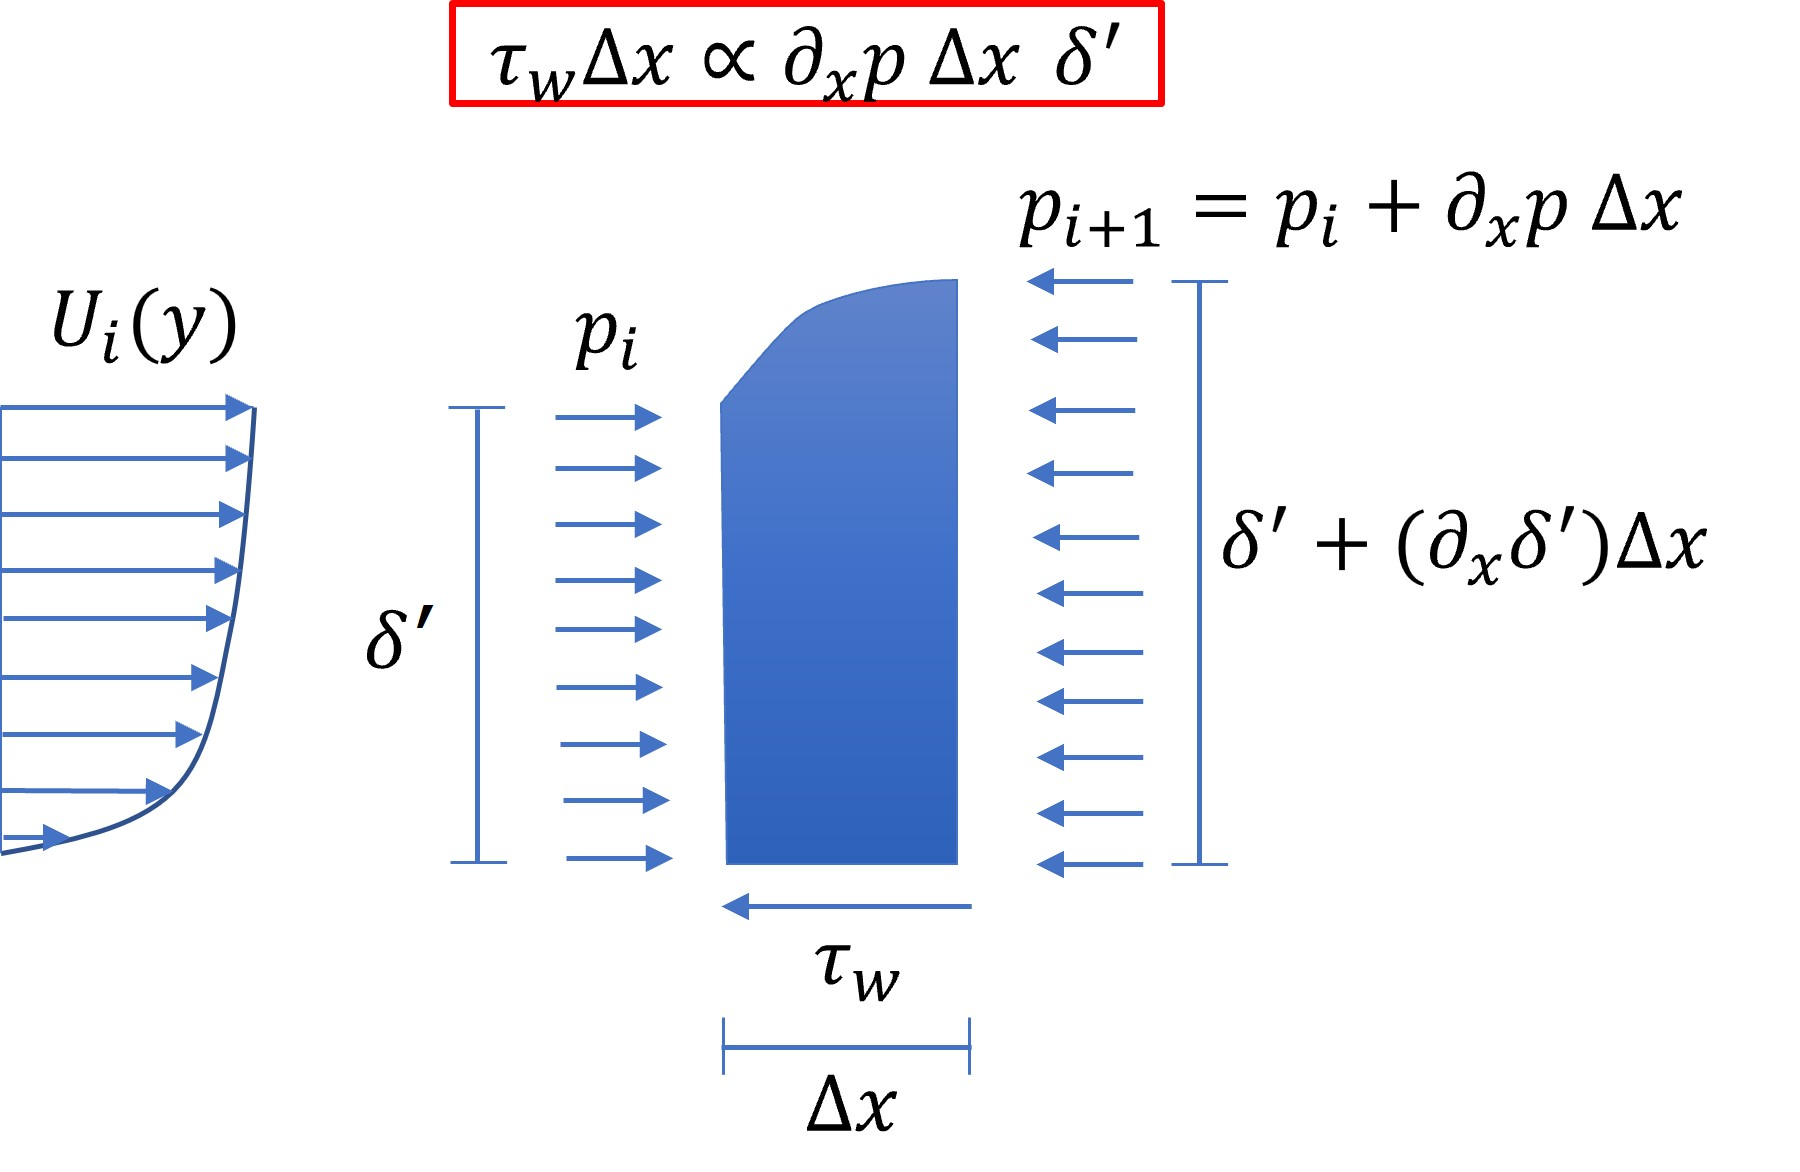
\includegraphics[width=0.90\textwidth]{imgs/schemes/scheme_beta.jpg}
    \caption{Stresses around a section of a BL.}
    \label{fig:scheme_beta}
\end{figure}

Integrating the streamwise momentum equation over the wall-normal direction, under several assumptions, it is possible to obtain an equation which relates the integral parameters $\delta^*$, $\theta$ and $\beta$, therefore, from an integral approach, the thickness $\delta \myprime$ is chosen equal to $\delta^*$. 



\section{Statistics}
In \textbf{Paper 1} we explore the statistical quantities of TBLs under APGs. The novelty respect to the available literature was in the high fidelity database used for the ZPG and APG TBLs. Both simulations show the development of the TBL from low Reynolds numbers such as those of previous numerical databases, and reach large Reynolds numbers such as those obtained in experiments. This characteristic works as a bridge to validate previous simulations as well as the current simulations, since they have been compared successfully with experimental data.
A benefit of numerical experiments is that the amount of quantities measured are larger than in experimental databases. This allows to have better measurements close to the wall and obtain decomposition such as spanwise spectra.

In Fig.~\ref{fig:U_uu_cap2}(a) we show the inner scaled $U$ and $\sqrt{\overline{u\myprime u\myprime}}$ for a $\Rey_{\tau}=500$, where the low Reynolds number simulations are already fully developed, while the experimental database does not have measurements. A higher $\Rey_{\tau}=2000$ is required by the experiments to have a fully developed near-equilibrium APG, and the LES ZPG and the new b1.4 simulation are able to achieve those Reynolds numbers.
The experimental data and b1.4 are in a similar range of $\beta$ and their statistics show a good agreement in the streamwise components.
The effects of the APG in $U$ show a lower $U^+$ for larger $\beta$ in the logarithmic region, and a larger effect in the wake region. At higher Reynolds numbers, the logarithmic region enlarges and the near-equilibrium APG and the ZPG profiles get closer.
In the turbulent perturbations, the near-wall or inner peak of $\sqrt{\overline{u\myprime u\myprime}}^+_{IP}$ grows in value with both the Reynolds number and the APG effects and its wall-normal position $y_{IP}^+$ seems to slightly increase with both APG and $\Rey$ effects. In \cite{Pozuelo_JFM_22} this trend is shown, where a filter was used to avoid saw-tooth jumps due to the wall-normal resolution close to the wall.
Larger Reynolds numbers allows for larger scales to live in the logarithmic/wake region and for a separation of the scales to be seen. This is first seen as lower decay in $\sqrt{\overline{u\myprime u\myprime}}$ in the ZPG in the logarithmic/wake region and a development of an outer peak for APG profiles. Larger $\beta$ increase the value of the outer peak of $\sqrt{\overline{u\myprime u\myprime}}$. The trends for the outer peak value and wall-normal position of the RS,  $\overline{u\myprime u\myprime}_{OP}$ and $y_{OP}$ where analysed in \cite{Pozuelo_JFM_22}. 


\begin{figure}
    \centering
    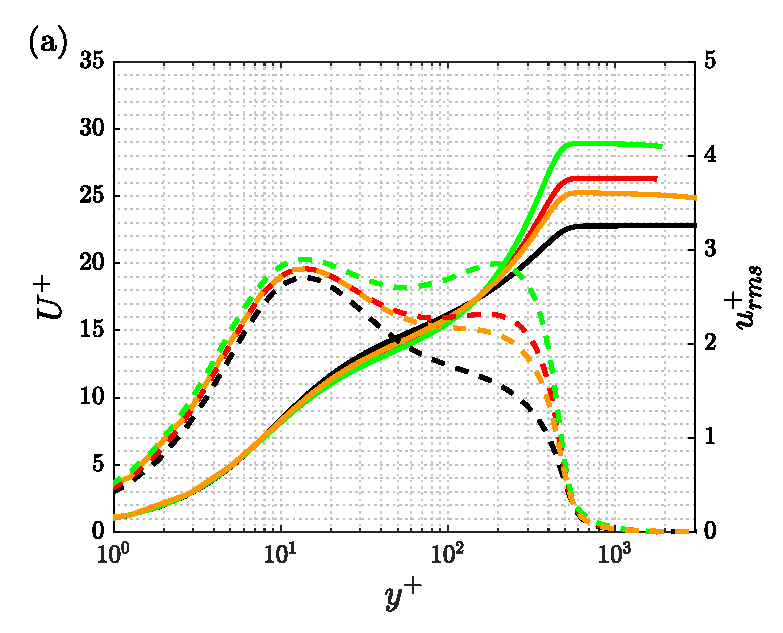
\includegraphics[width=0.49\textwidth]{imgs/stats/U_uu_a.eps}
    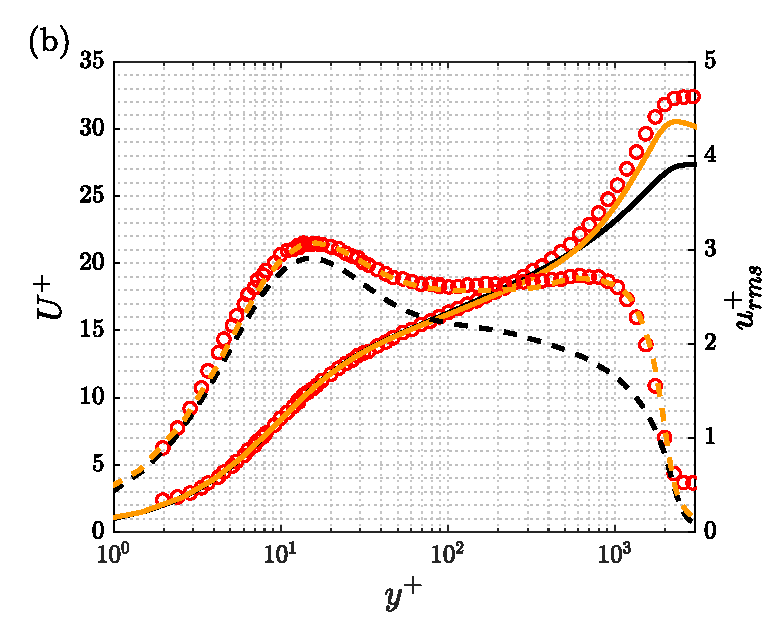
\includegraphics[width=0.49\textwidth]{imgs/stats/U_uu_b.eps}
    \caption{Mean streamwise $U$ (solid lines) and streamwise root mean square $u_{rms}$ or strandard deviation of the streamwise velocity (dashed lines). Wall-normal profiles taken at: (a) $\Rey_{\tau}=500$, (b) $\Rey_{\tau}=2100$. }
    \label{fig:U_uu_cap2}
\end{figure}

\subsection{Cf}

\subsection{RS}


\subsection{Spectral decomposition}
To have a better understanding on the perturbations we can use some mathematical tools such as the decomposition of the spatial-temporal signal using correlations, orthogonal modes, coherent structures, etc.
The use of orthogonal modes allows to decompose the energy of the perturbations into each mode in an unique way, so the sum of the energy contained in all the modes is equivalent to the total energy of the perturbations. 

In signal analysis an orthogonal decomposition which is commonly used is the Fourier decomposition which enables to look for phenomena that repeats with a certain time or spatial frequency. The energy or power associated with each mode is called energy spectra (if the signal is finite such as pulses) or power spectra (if the signal is such as sinusoidal waves, whose domain and energy is not finite, however its power is). Remember that the power is the ratio of the energy over time, where the time goes to infinity (in the case of using temporal series).
Since we are dealing with signals which are periodic in the homogeneous dimension $z$ and are not limited in time, we will use the terminology of power spectra (PS) instead of energy spectra. 
The modes in $z$ have a wavenumber $k_z$ and a wavelength $\lambda_z=2\pi/L_z$ where $L_z$ is the spanwise period of the domain. The same analysis can be applied in time, where we will use $k_t$ and $\lambda_t$.
For a signal $x(t)$, with $X(k_t)$ being its Fourier transform, the power of each mode is $|X(k_z)|^2$, the squared amplitude of the mode. For a perturbation velocity, the power can be calculated as,
\begin{equation}
    PS_{u_i\myprime u_j\myprime}(k_z) = \mathcal{F}(u_i \myprime)  \mathcal{F}^*(u_j \myprime),
    \label{eq:power_sp}
\end{equation}
where $\mathcal{F}()$ is the Fourier transform and $\mathcal{F}^*()$ represents the complex conjugate and the definition has been expanded to include the power spectra of the quantity $\langle u_i\myprime u_j\myprime \rangle_{z}$, also known as cospectra.
Using the properties of the Fourier transform, the multiplication in Fourier space represented in Eq.~\ref{eq:power_sp} represents the Fourier transform of the two-point correlation function $\mathcal{R}_{u_i\myprime, u_j\myprime}(\delta z)=u_i\myprime \star u_j\myprime$, where $\delta z$ is the lag or distance between the two points where we look for the correlation of their velocity perturbations. According to the Wiener--Khinchin theorem, we can calculate the PS through as the Fourier transform of $\mathcal{R}_{u_i\myprime, u_j\myprime}$ or from the power spectra throught the inverse Fourier transform $\mathcal{F}^{-1}()$ we can obtain the two-point correlation function.

Note that for velocity perturbations, since Fourier modes are orthogonal, the sum of the PS for all the modes is equal to the averaged Reynolds stress,
\begin{equation}
    \langle u_i\myprime u_j\myprime \rangle_{z} = \sum_{k_z} PS_{u_i\myprime u_j\myprime}(k_z)
\end{equation}

This step can be performed for each time step and averaged over time to obtain $\langle\langle u_i\myprime u_j\myprime \rangle_{z}\rangle_{t} = \overline{u_i\myprime u_j\myprime}$ or it can also be the result of a 2D spectral decomposition in both time and $z$, where the sum extends to all the spatial and temporal modes.

The PS is useful for discrete systems, and it is the first step when we calculate numerically the spectra of a the Reynolds-stresses. It is also interesting to see how the power spectra is distributed along the wavenumbers or the wavelengths, obtaining a power spectral density (PSD).
The average in time of the PSD in wavenumbers is $\phi_{u_i\myprime u_j\myprime}=\langle PS \rangle_t/\mathrm{d} k_z$ while the average in time PSD in wavelengths is $\psi_{u_i\myprime u_j\myprime}= \langle PS \rangle_t/\mathrm{d} \lambda_z$. Both densities can be linked using $\mathrm{d}(\lambda_z) = \mathrm{d}(2\pi/k_z) = -2\pi\mathrm{d}k_z/k_z^2$:

\begin{equation}
    \psi_{u_i\myprime u_j\myprime} = 
    \frac{ \langle PS_{u_i\myprime u_j\myprime} \rangle_t}{\mathrm{d} \lambda_z} =
    -\frac{ \langle PS_{u_i\myprime u_j\myprime} \rangle_t}{\mathrm{d} k_z} \frac{k_z^2}{2\pi},
\end{equation}
where the minus sign is taking care by inverting the limits of integration to obtain the total RS (small to large wavenumbers is equivalent to integrate from large to small wavelengths).

\begin{equation}
\label{eq:sum_ps}
    \overline{u_i\myprime u_j\myprime} = 
    \int_{k_z=k_0}^{k_z=k_{N}}   \phi_{u_i\myprime u_j\myprime}  ~ \mathrm{d} k_z =
    \int^{\lambda_z = 2\pi/k_0}_{\lambda_z = 2\pi/k_{N}}  \psi_{u_i\myprime u_j\myprime}  ~ \mathrm{d} \lambda_z
\end{equation}

In Fig.~\ref{fig:PS_PSD} we show for a ZPG TBL, different representations of the PSD of $\overline{u\myprime u\myprime}$ where the image with the black contours represent a streamwise profile at $\Rey_{\tau}=2000$ while the red contours are taken at a position where $\Rey_{\tau}=500$.

\begin{figure}[h!]
\centering
% \captionsetup{width=0.99 \textwidth}
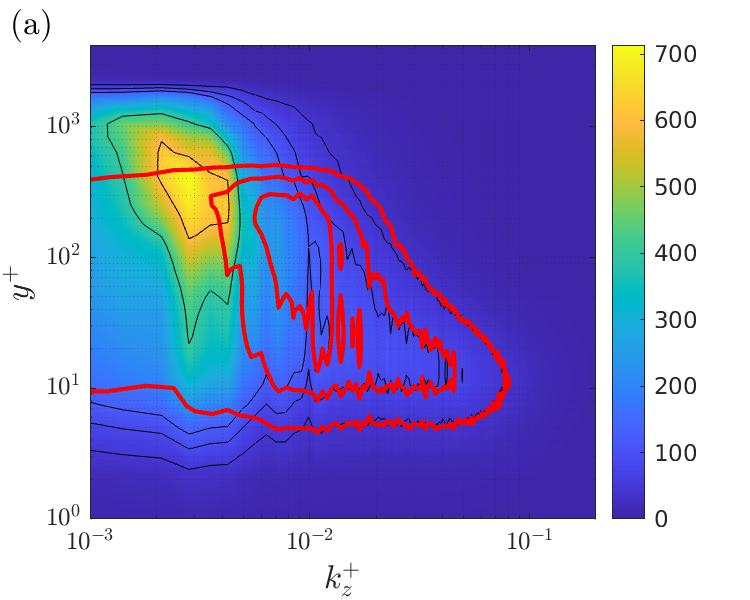
\includegraphics[width=0.32\textwidth ]{imgs/spec/ZPG_Ret_500_2000_PSdkz_kz_ltau_y_ltau.jpg}
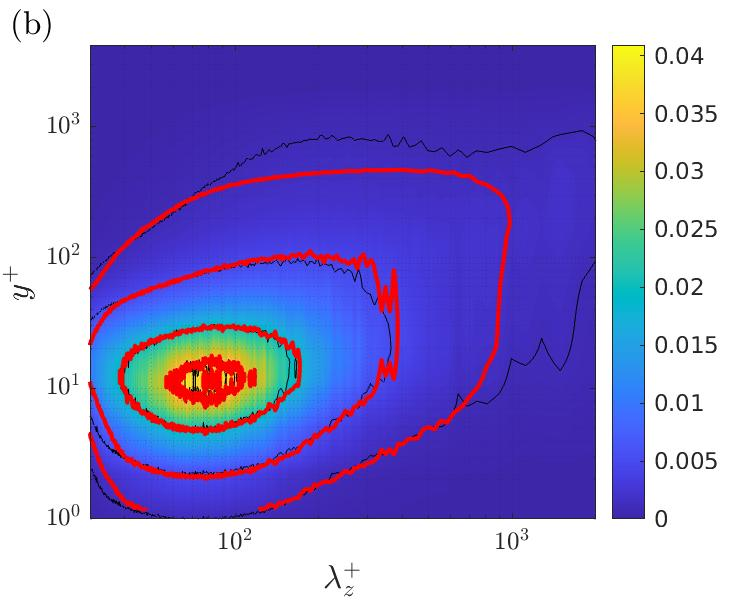
\includegraphics[width=0.32\textwidth]{imgs/spec/ZPG_Ret_500_2000_PSdlambdaz_lambdaz_ltau_y_ltau.jpg}
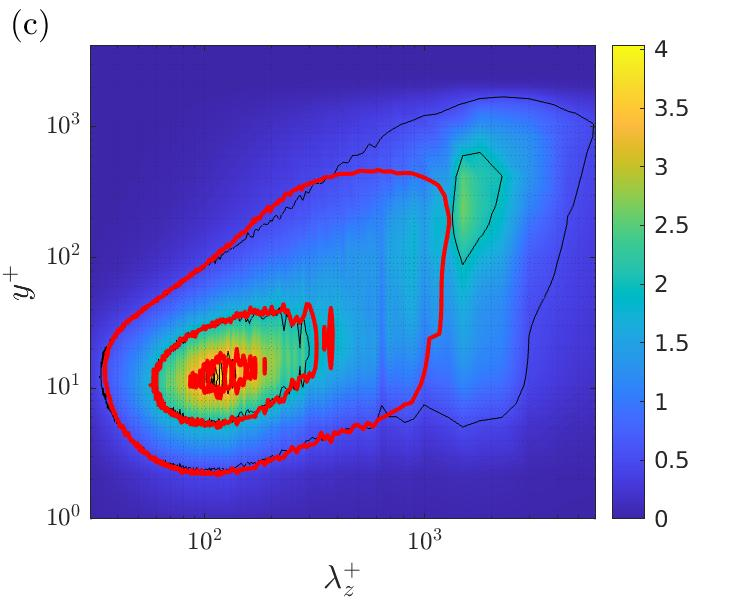
\includegraphics[width=0.32\textwidth]{imgs/spec/ZPG_Ret_500_2000_kPSdkz_lambdaz_ltau_y_ltau.jpg}
\caption{ \label{fig:PS_PSD} Spanwise spectra of the streamwise Reynolds stress $\overline{uu}(y)$. (a) Power spectral density $\phi_{u\myprime u\myprime}(y,k_z)$; (b) Power spectral density $\psi_{u\myprime u\myprime}(y,\lambda_z)$; (c) premultiplied power spectral density $k_z\phi_{u\myprime u\myprime}$. Wavenumbers, wavelengths, wall-normal position and power spectra scaled in viscous units.}
\end{figure}
% contours: Retau 2000: [40 80  120 400 600]; [0.001 0.005 0.02 0.035 0.04] ;  [ 0.5 2 3.5]; 
% contours: Retau  500: [40 80  120        ]; [0.001 0.005 0.02 0.035 0.04] ;  [ 0.5 2 3.5]; 

The PS and the PSD in the wavenumbers $\phi_{u\myprime u\myprime}(y,k_z)$ present the same features as in Fig.~\ref{fig:PS_PSD}(a), since $dk_z$ or $dk_z^+$ are constant factors that does not vary with the wavenumbers. It shows a high content of power/energy of structures with a very low wavenumber which are very wide. It is possible to see similarities in the contours at different Reynolds numbers (red and black lines) in the region of high wavenumbers (small scales), although the energetic level is very low compared to that of the low wavenumbers (large scales).
The PSD in wavelengths $\phi_{u\myprime u\myprime}(y,\lambda_z)$ is represented in Fig.~\ref{fig:PS_PSD}(b) and it focuses on the small scales. It shows that the density of power/energy in the small scales (short wavelengths) is very similar at different Reynolds numbers and larger than the PSD of the wider scales (large $\lambda_z^+$). 
From Fig.~\ref{fig:PS_PSD}(a) and (b) we see that the small scales have a small content of the total RS energy, but their small size make the density in waveleghts to be very concentrated, while for the wider scales is the opposite, the energy they contain is very large, but their big size make the PSD to be very low or disperse.
If we write both PSD as a function of $\phi_{u\myprime u\myprime}$, in Fig.~\ref{fig:PS_PSD}(a) we show $\phi_{u\myprime u\myprime}$ while in Fig.~\ref{fig:PS_PSD}(b) it would be $k_z^2 \phi_{u\myprime u\myprime}$, the premultiplication factor $k_z^2$ is responsible to augment the effects of the small scales while diminishing the effects of the large scales. Fig.~\ref{fig:PS_PSD}(c) shows $k_z \phi_{u\myprime u\myprime}$, whose effect equilibrates the effect of the large and small scales obtaining a better visualization of both scales.

The premultiplied PSD $k_z \phi_{u\myprime u\myprime}$ is widely used and it has a geometrical explanation.
Since the range of energetic scales is so large that we observe very small scales close to the wall and very large scales of the size of $\delta_99$, the use of logarithmic axis helps to expand the region of small $\lambda_z$ and the region close to the wall.
If we use logarithms in the definition of wavelength, $ \mathrm{ln}(\lambda_s) = \mathrm{ln}(2\pi) - \mathrm{ln}(k_z)$, and apply the differential, $\mathrm{d}(\mathrm{ln} \lambda_z) = -\mathrm{d}(\mathrm{ln} k_z)$, and together with $\mathrm{d}k_z = k_z \mathrm{d}(\mathrm{ln} k_z)$ can be substituted in Eq.~\ref{eq:sum_ps} to obtain:
\begin{equation}
    \overline{u_i\myprime u_j\myprime} = 
    \int_{k_0}^{k_{N}}   \phi_{u_i\myprime u_j\myprime}  ~ \mathrm{d} k_z = 
    \int_{k_0}^{k_{N}}   \phi_{u_i\myprime u_j\myprime} k_z  ~ \mathrm{d}( \mathrm{ln} k_z) = 
    \int^{\lambda_0}_{\lambda_{N}}   \phi_{u_i\myprime u_j\myprime} k_z ~ \mathrm{d}( \mathrm{ln} \lambda_z).
\end{equation}

The premultiplication by $k_z$ can be seen here as a factor to visualize a corrected area after scaling the axis with a logarithmic scale.
From here on the PSD will always be represented in its premultiplied form $k_z\phi$ to have a clear visualization of the effects of large and small scales at the same time.

\subsubsection{Wide scales in turbulence. Channel Flows}
It has been seen that the big scales contains a large part of the turbulent energy, although the density spectral density is low.
When we model the turbulent flow, the size of the domain imposes a limit on the size of the scales that can be simulated. In a periodic domain, the largest scale corresponds to $L_x$ and the wider scale to $L_z$. Bigger scales will be seen as infinit in size because of the periodicity, and the spectral energy will be stored in the zero-wavenumbers.

The energy contained in the zero-wavenumbers is affected by the averaging.

If the size of the domain is not large or wide enough, the bigger turbulent scales will not be able to be captured and the energetic spectrum will not be correct, affecting the total statistics such as the Reynolds stresses and the mean velocity profiles.
Many analysis on the size of the domain has been performed on canonical turbulent channel flows for it simplicity.
\highlight{Minimal channels are those small domains that assure }
On the other way, the largest scales in channel flows where looked for in \highlight{CITAR ADRIAN que descubrieron bla bla}.
The study on the wider scales was based on two-point correlations, but no other study similar to \highlight{CITAR ADRIAN} was performed in the spanwise direction.

To have a better understunding of the wide scales obtained in APG TBLs and the effects of the domain size, we decided to study first the effect on wide-channels.
Three simulations were performed of turbulent channel flows at $\Rey_{\tau} = 550 $ under similar conditions, with the only excemption the width of their domains which was doubled from one channel to another as it can be seen in \highlight{Tabla de los channel}.
 


\subsubsection{Spectral results on APG}

In \textbf{Paper 1} the 1D spanwise spectra and the 2D spanwise and temporal spectra of the APG TBL where shown and compared to those of a ZPG TBL \citep{EAmorZPG}. By using percentage contours it was possible to show a similar behaviour in the mild APG and the ZPG simulations at different Reynolds numbers in the small-scale energy region close to the wall around an spectral near-wall peak or spectral inner peak (sIP) at $y^+\approx 15$ and $\lambda_z^+\approx 120$. Another region with similar shape is in the wake region with an spectral outer peak that seemed to scale with the Reynolds number.
Another region is that of small-scale energy in the wake region, which is only present in the APG simulation and not in the ZPG case.

\begin{itemize}
    \item show pcolor con APG y ZPG de uu, uv en Retau 500 y 2000
\end{itemize}

The spectra shows a similar region of small-scale energy close to the wall which is responsible of the near-wall peak the RS $\overline{u\myprime u\myprime}$. The effects of $\Rey$ and $\beta$ increase the value of $\overline{u\myprime u\myprime}_{IP}^+$, even if the most of the spectra is similar for APG and ZPG at different Reynolds numbers.
The outer-spectral peak in $k_z\phi_{uu}$ is also responsible of most of the energy contained in the ZPG in the wake region, and increasing $\beta$ it increases the energy to the point of growing the outer peak in $\overline{u\myprime u\myprime}_{OP}^+$. This behaviour is similar in the other components of the RS tensor, where at higher $\Rey$ numbers there are larger and energetic scales acting on the wake region and influencing all across the TBL.

\subsubsection{Scaling of APG spectrum}

In \textbf{Paper 2} we try to understand the trends of the inner and outer peaks in $\overline{u\myprime u\myprime}$ shown in \textbf{Paper 1}. Why the inner scaled inner-peak grows with the Reynolds numbers and with the APG effects. Is it still correct to use viscous scaling?. 
We perform a scaling analysis of the different energetic scales of the power spectral density for both ZPG and APG simulations and at different Reynolds numbers.
First we start from the features observed in $k_z\phi_{u\myprime u\myprime}$ which are an spectral near-wall/inner peak (sIP) and an spectral outer peak (sOP). The data is scanned to look for the maxima at a certain wall-normal position and the maxima at a certain frequency. Since $k_z\phi_{u\myprime u\myprime}$ is saved in a rectangular matrix, it is equivalent to obtain the maxima along columns and the maxima along rows.
At high Reynolds number the separation of scales even in ZPG TBLs, allows to distinguish clearly the presence of 2 maximal points for $\Rey_{\tau}>500$. Other techniques could be used to detect the local maxima, but this method was obtaining satisfactory results, specially the values of $f(y)=max(k_z\phi(k_z, y))_{k_z}$ since that function presents less noise and it is shown in \highlight{ Fig.~\ref{fig:scaling_OP} figura de los escalados de los picos} that once the Reynolds number is enough to have separation of scales, the outer peak clearly separates in the wall-normal direction from the spectral near-wall peak.
Once sIP and sOP are located in $k_z\phi(k_z, y)$, (usually we represent with $\lambda_z$), we try the inner and outer length scalings used in \textbf{Paper 1} to scale $\overline{u\myprime u\myprime}(y)$.
It is shown that the viscous length $\ell_{\tau}$ scales the size of the spanwise scales of the sIP $\lambda_{z, sIP}^+$ as well as the wall-normal position $y^+_{sIP}$.
The same method is used for the spectral outer peak. The outer scales $\delta^*$ and $\delta_{99}$ were used to scale independently the wall-normal location $y_{sOP}$ and the size of the scales $\lambda_{z, sOP}$.
In previous studies such as \cite{Kitsios2017} the $\delta^*$ scaling was successful for the $y_{OP}$ as well as for $y_{sOP}$ at much higher $\beta$, however, $\lambda_z$ was also scaled with the same scaling.
In \cite{tanarro_2020}, the outer scaling was performed with $\delta_{99}$ for both $y$ and $\lambda_z$, and the values of $\lambda_{z,sOP}$ were better collapsed than using $\delta^*$ as in \cite{Kitsios2017}.
Taking into account this previous studies, we allowed $y$ and $\lambda_z$ to have different length scalings, and found the optimal collapse of the region around the spectral outer peak using $y/\delta^*$ and $\lambda_z/\delta_{99}$.

Once we obtained the scalings for the wall-normal position and size of the scales for both sIP and sOP, we looked the region around those peaks using the respective scalings, obtaining a good collapse, however there was another region to investigate, which is the region of small-scale energy in the wake region.
Different scalings were tried for $\lambda_z$ looking to match the vertical part of the energetic contours of the APG simulation at different $\Rey$.
We observed that using $\lambda_z/\delta^*$, there is a collapse around $\lambda_z/\delta^*=0.3$. It could be argued that the scaling evolves gradually at different $\lambda_z$ up to the region around the sOP that clearly scale using $\lambda_z/\delta_{99}$.
To have a better idea of how big was the contribution of the small-scale energy in the wake region, but also to understand what is the influence of the large scales in the near-wall region, we tried to accumulate the energy from small to large scales for all the wall-normal positions. In a matrix containing the $PS(y,k_z)$, this is equivalent to do a cumulative sum $cumsum(PS(y,k_z))_{k_z}$ along $k_z$.
In \cite{EAmorZPG}, they limited a rectangular region around sIP, to probe that inner scaled energy in this region does not vary with the Reynolds number, but we have seen that there are different scalings at different heights of the TBL, therefore, the rectangular domain to integrate over $\lambda_z$ and $y$ may not be the optimal tool for this analysis.

With the idea of looking for the contribution of small and large scales using a cumulative sum, and thinking that the accumulated energy would be in a certain scaling that probably would change with $\Rey$ effects, we thought of the percentual contribution of energy, or the marginal contribution of energy.
For a continuous PSD, the marginal contribution of energy (MCE) is defined as in Eq.~\ref{eq:MCE_cap2} and gives the percentual level of energy added by scales up to a wavenumber $k_{z,c}$ respect to the total value which would be $\overline{u_i\myprime u_j\myprime}$ at the same $y$.

\begin{equation}
\mathrm{MCE} = \int_{k_{z,c}}^{\infty} \phi_{u_iu_j} \mathrm{d} k_z \ \bigg/ \int_{0}^{\infty} \phi_{u_iu_j} \mathrm{d} k_z,
\label{eq:MCE_cap2}
\end{equation}

If we draw the $10\%, 20\%,...,$ contours, it is easy to show the regions where certain election of length and energy scales are valid, since the contours will be parallel where the scales contributes in the same way to the total RS. And they will start to diverge when the scaling is not appropriate.
Where the scaling is independent of $\Rey$, the contours for different $\Rey$ at the same MCE level in that region, will collapse, otherwise they will start to separate indicating for example that the influence of large-scale motions is affecting that region.
All of this is shown in \textbf{Paper 2} in more detail.
Answering why $\overline{u\myprime u\myprime}_{IP}^+$ grows with the $\Rey$ and $\beta$, the answer is that at higher $\Rey$ the influence of scales of size $\delta_{99}$ or larger, influence the near-wall region, and this influence is larger at with larger $\beta$. At this range of $\beta$, the viscous scaling is still valid, although certain modifications could be done taking into account the influence of the large scales.
At larger $\beta$, the flow is near-detachment and the viscous scaling is no longer applicable.











%
%===============================================================================
\chapter{Transport of energy between turbulent scales}
%===============================================================================
%

\subsubsection{Interscale transport of energy.}

From the Reynolds transport equation or the KE, MKE and TKE budget equations, it was possible to obtain a term called ``Production'' which is composed by the RS and the mean velocity gradients, and it can be interpreted as a source of turbulent energy in the TKE equation and a sink in the MKE equation. Their contribution are cancelling each other when added to obtain the KE equation.

Following this idea, a similar term is looked for in the Reynolds-stress transport equations, that may indicate the transfer of energy between large scales and small scales.
In order to obtain such a decomposition, we follow the steps in \cite{PRL2018_Kawata, JFM2019_kawata_alfredsson}, where the perturbation velocity is further decomposed in a contribution from large scales $u_i^L$ and a contribution from small scales $u_i^S$, where the separation between large or small scales is made by a cutoff frequency/wavenumber in Fourier space $k_{z,c}$.
\begin{equation}
    \label{eq:intersc_decomp}
    u_i\myprime = u_i^L + u_i^S,
\end{equation}
\begin{equation}
    \label{eq:intersc_decomp}
    \langle u_i\myprime u_j\myprime \rangle_z = 
    \langle u_i^L u_j^L \rangle_z + 
    \langle u_i^S u_i^S \rangle_z
\end{equation}
\begin{equation}
    \label{eq:intersc_decomp}
    \overline{u_i\myprime u_j\myprime} = 
    \overline{ u_i^L u_j^L} + 
    \overline{ u_i^S u_i^S}
\end{equation}

\begin{equation}
    \label{eq:intersc_decomp}
    \overline{ u_i^L u_j^S} = 
    \overline{ u_i^S u_j^L} = 0
\end{equation}



\begin{itemize}
    \item 
\end{itemize}
%
%===============================================================================
\chapter{Numerical experiments on high Reynolds numbers flat plate turbulent boundary layers}
%===============================================================================
%
\section{SIMSON}

\section{Equations}



\section{MPI}


\section{LES}


\section{BCs}
%===============================================================================
\chapter{Conclusions and outlook}
%===============================================================================
%
%===============================================================================
% %===============================================================================

% This chapter is meant for testing the correct referencing of figures, equations
% and tables.

% % equations
% %
% \begin{equation}
% 	1 + 1 = 2
% 	\label{eq:test_eq1}
% \end{equation}

% \begin{align}
% 	2 + 2 = 4
% 	\label{eq:test_eq2}
% \end{align}

% \begin{equation}
% 	3 + 3 = 6
% 	\label{eq:test_eq3_intro}
% \end{equation}

% % tables
% %
% \begin{table}
% 	\centering
% 	\begin{tabular}{c}
% 		1
% 	\end{tabular}
% 	\caption{Test table 1}
% 	\label{tab:test_tab1}
% \end{table}

% \begin{table}
% 	\centering
% 	\begin{tabular}{c}
% 		2
% 	\end{tabular}
% 	\caption{Test table 2}
% 	\label{tab:test_tab2}
% \end{table}

% \begin{table}
% 	\centering
% 	\begin{tabular}{c}
% 		3
% 	\end{tabular}
% 	\caption{Test table 3}
% 	\label{tab:test_tab3_intro}
% \end{table}

% % figures
% %
% \begin{figure}[h!]
% 	\centering
% 	test figure 1
% 	\caption{Test figure 1}
% 	\label{fig:test_fig1}
% \end{figure}

% \begin{figure}[h!]
% 	\centering
% 	test figure 2
% 	\caption{Test figure 2}
% 	\label{fig:test_fig2}
% \end{figure}

% \begin{figure}[h!]
% 	\centering
% 	test figure 3
% 	\caption{Test figure 3}
% 	\label{fig:test_fig3_intro}
% \end{figure}

% test references
% %
% \hrule
% \begin{itemize}
% 	\item reference to equation 1: \eqref{eq:test_eq1}
% 	\item reference to equation 2: \eqref{eq:test_eq2}
% 	\item reference to equation 3: \eqref{eq:test_eq3_intro}
% \end{itemize}
% \hrule
% \begin{itemize}
% 	\item reference to table 1: \eqref{tab:test_tab1}
% 	\item reference to table 2: \eqref{tab:test_tab2}
% 	\item reference to table 3: \eqref{tab:test_tab3_intro}
% \end{itemize}
% \hrule
% \begin{itemize}
% 	\item reference to figure 1: \eqref{fig:test_fig1}
% 	\item reference to figure 2: \eqref{fig:test_fig2}
% 	\item reference to figure 3: \eqref{fig:test_fig3_intro}
% \end{itemize}
% \hrule

%===============================================================================
% Acknowledgments
%===============================================================================
%
\begin{acknowledgements}
% 	We would like to thank Gigi and SCIgen - An Automatic CS Paper Generator%
% 	\footnote{\url{https://pdos.csail.mit.edu/archive/scigen}}.
I would like to thank Ricardo Vinuesa and Philipp Schlatter first, without them I wouldn't have lived this wonderful adventure,
conducting my PhD studies in KTH and start a new life in a beautiful country such as Sweden.
To all those friends, old and new PhD students and professors that have made my stay so enjoyable.
And to my family in Spain and those that I got to consider family in Sweden for your support and love.
% Qiang Li, a collaborator in my publications, but also a mentor, always encouraging me and ready to help. They have helped and guided me through my academic work and have always been there to share their knowledge an experience.
% I also have to thank all those PhD's and professors that have made the life in the office so wonderful, in spite of the huge change that covid brought to our lifes.
% Luca, Simon, Valerio and Vitor, with whom I lived my first "western" adventure. And the list goes on and on.
% My family and friends in Spain that missed me so much, and my small "family" in Sweden for your moral support in good and dark times.
\end{acknowledgements}



%===============================================================================
% References
%===============================================================================
%
\bibliographystyle{jfm}
\bibliography{thesis}
%
% \IfFileExists{overview.bbl}{\graphicspath{{imgs/}}

%===============================================================================
\chapter{Introduction}
%===============================================================================
%
\input{Chapter1}

%-------------------------------------------------------------------------------
\section{Our Contribution}
%
\thesisstructure Part I of the thesis contains 4 chapters. 
In chapter 2 we provide a basic introduction to fluid mechanics and turbulent boundary layers affected by adverse pressure gradients.
From the observations and expected phenomenology to the mathematical equations that describe the mechanics of the flow, and the equations that we use to approach the study of turbulent flows.
Chapter 3 introduces one of the biggest simulations on near-equilibrium turbulent boundary layers performed so far. The high-quality data on adverse-pressure gradient turbulent boundary layers is used to asses different phenomena such as the effects of adverse pressure gradients on the friction coefficient or the scaling factors of the turbulent scales using spectral decomposition.
Chapter 4 deals with the problem of the energetic exchange between turbulent scales, where we discuss the mathematical approach and its significance.
Finally in Chapter 5 we present the numerical code used for the simulations, and some details of the set up for the large simulation that we have presented.

%===============================================================================
\chapter{Boundary layers, turbulence and pressure gradients}
%===============================================================================
%
\input{Chapter2}
%===============================================================================
\chapter{Effects of adverse pressure gradients in turbulent boundary layers}
%===============================================================================
%
\input{Chapter3}
%
%===============================================================================
\chapter{Transport of energy between turbulent scales}
%===============================================================================
%
\input{Chapter4}
%
%===============================================================================
\chapter{Numerical experiments on high Reynolds numbers flat plate turbulent boundary layers}
%===============================================================================
%
\input{Chapter5}
%===============================================================================
\chapter{Conclusions and outlook}
%===============================================================================
%
%===============================================================================
% %===============================================================================

% This chapter is meant for testing the correct referencing of figures, equations
% and tables.

% % equations
% %
% \begin{equation}
% 	1 + 1 = 2
% 	\label{eq:test_eq1}
% \end{equation}

% \begin{align}
% 	2 + 2 = 4
% 	\label{eq:test_eq2}
% \end{align}

% \begin{equation}
% 	3 + 3 = 6
% 	\label{eq:test_eq3_intro}
% \end{equation}

% % tables
% %
% \begin{table}
% 	\centering
% 	\begin{tabular}{c}
% 		1
% 	\end{tabular}
% 	\caption{Test table 1}
% 	\label{tab:test_tab1}
% \end{table}

% \begin{table}
% 	\centering
% 	\begin{tabular}{c}
% 		2
% 	\end{tabular}
% 	\caption{Test table 2}
% 	\label{tab:test_tab2}
% \end{table}

% \begin{table}
% 	\centering
% 	\begin{tabular}{c}
% 		3
% 	\end{tabular}
% 	\caption{Test table 3}
% 	\label{tab:test_tab3_intro}
% \end{table}

% % figures
% %
% \begin{figure}[h!]
% 	\centering
% 	test figure 1
% 	\caption{Test figure 1}
% 	\label{fig:test_fig1}
% \end{figure}

% \begin{figure}[h!]
% 	\centering
% 	test figure 2
% 	\caption{Test figure 2}
% 	\label{fig:test_fig2}
% \end{figure}

% \begin{figure}[h!]
% 	\centering
% 	test figure 3
% 	\caption{Test figure 3}
% 	\label{fig:test_fig3_intro}
% \end{figure}

% test references
% %
% \hrule
% \begin{itemize}
% 	\item reference to equation 1: \eqref{eq:test_eq1}
% 	\item reference to equation 2: \eqref{eq:test_eq2}
% 	\item reference to equation 3: \eqref{eq:test_eq3_intro}
% \end{itemize}
% \hrule
% \begin{itemize}
% 	\item reference to table 1: \eqref{tab:test_tab1}
% 	\item reference to table 2: \eqref{tab:test_tab2}
% 	\item reference to table 3: \eqref{tab:test_tab3_intro}
% \end{itemize}
% \hrule
% \begin{itemize}
% 	\item reference to figure 1: \eqref{fig:test_fig1}
% 	\item reference to figure 2: \eqref{fig:test_fig2}
% 	\item reference to figure 3: \eqref{fig:test_fig3_intro}
% \end{itemize}
% \hrule

%===============================================================================
% Acknowledgments
%===============================================================================
%
\input{acknowledgements}


%===============================================================================
% References
%===============================================================================
%
\bibliographystyle{jfm}
\bibliography{thesis}
%
% \IfFileExists{overview.bbl}{\input{overview.bbl}}{}
}{}
}{}



%-------------------------------------------------------------------------------
% Comment the following command if you do not want a separate page for Part II
% in the table of contents
%
\tocpagebreak


%===============================================================================
% Part II: Papers
%===============================================================================
%
\part{Papers}

%-------------------------------------------------------------------------------
% Summary of the papers
%
\makepapersummary
\cleardoublepage

%-------------------------------------------------------------------------------
% Paper 1
%
%------------------------------------------------------------------------------
% Define title, author(s), affiliation and publishing status
%
\papertitle[LES of a moderate-APG TBL at high $Re$] % Short title used in headlines (optional)
{%
  An adverse-pressure-gradient turbulent boundary layer with nearly-constant $\boldsymbol{\beta \simeq 1.4}$ up to $\boldsymbol{Re_{\theta} \simeq 8,700}$% THE COMMENT SYMBOL AT THE END OF THIS LINE IS NEEDED
}%
%
\papertoctitle{An adverse-pressure-gradient turbulent boundary layer \\with nearly-constant ${\beta \simeq 1.4}$ up to ${Re_{\theta} \simeq 8,700}$} % Title for toc
%
\paperauthor[R. Pozuelo, Q. Li, P. Schlatter \& R.Vinuesa] % Short authors used in headlines and List Of Papers
{%
  Ram\'on Pozuelo$^1$, Qiang Li$^1$, Philipp Schlatter$^1$ and Ricardo Vinuesa$^1$%
}%
%
%\listpaperauthor{A. Skywalker \& D. Vader}% (optional) Short authors used in List Of Papers
%
\paperaffiliation
{%
  $^1$ FLOW, Engineering Mechanics, KTH Royal Institute of Technology, SE-100 44 Stockholm, Sweden
}%
%
\paperjournal[J.~Fluid Mech.] % Short publish info used in List Of Papers
{%
	Journal of Fluid Mechanics%
}%
%
\papervolume{939}%
%
\papernumber{1}%
%
\paperpages{A34}%
%
\paperyear{2022}%
%
\papersummary%
{% Insert summary of the paper here (used in introduction) 
	A new adverse-pressure-gradient turbulent boundary layer simulation is presented.
	The largest Reynolds number obtained in the simulation makes it possible to compare and validate results with those of experiments at similar pressure-gradient conditions.
	The large database obtained make it possible to analyze 2-dimensional statistics as
	well as spectral information in time and spanwise directions.
}%
%
\graphicspath{{paper1/figs}}%
%
%
%===============================================================================
%                            BEGIN PAPER
%===============================================================================
%
\begin{paper}

\makepapertitle

%------------------------------------------------------------------------------
% Abstract
%------------------------------------------------------------------------------
%
\begin{paperabstract}
In this study, a new well-resolved large-eddy-simulation (LES) of an incompressible near-equilibrium adverse-pressure-gradient (APG) turbulent boundary layer (TBL) over a flat plate is presented. In this simulation, we have established a near-equilibrium APG over a wide Reynolds-number range. In this so-called region of interest (ROI), the Clauser--Rotta pressure-gradient parameter $\beta$ exhibits an approximately constant value of around 1.4, and the Reynolds number based on momentum thickness reaches $\Rey_{\theta}=8700$. To the authors’ knowledge, this is to date the highest $\Rey_{\theta}$ achieved for a near-equilibrium APG TBL under an approximately constant moderate APG.  
We evaluated the self-similarity of the outer region using two scalings, namely the Zagarola--Smits and an alternative one based on edge velocity and displacement thickness. 
Our results reveal that outer-layer similarity is achieved, and the viscous scaling collapses the near-wall region of the mean flow in agreement with classical theory.
Spectral analysis reveals that the APG displaces some small-scale energy from the near-wall to the outer region, an effect observed for all the components of the Reynolds-stress tensor, which becomes more evident at higher Reynolds numbers.
Generally, the effects of the APG are more noticeable at lower Reynolds numbers. For instance, the outer peak of turbulent-kinetic-energy (TKE) production is less prominent at higher $Re$. 
While the scale separation increases with $\Rey$ in zero-pressure-gradient (ZPG) TBLs, this effect becomes accentuated by the APG. Despite the reduction of the outer TKE production at higher Reynolds numbers, the mechanisms of energization of large scales are still present. 
\end{paperabstract}


%------------------------------------------------------------------------------
% Article
%------------------------------------------------------------------------------
%
% % \documentclass{jfm}

% % 
\usepackage{graphicx}% Include figure files
\usepackage{dcolumn}% Align table columns on decimal point
\usepackage{bm}% bold math
%\usepackage[mathlines]{lineno}% Enable numbering of text and display math
%\linenumbers\relax % Commence numbering lines

\usepackage[utf8]{inputenc}
\usepackage[T1]{fontenc}
\usepackage{mathptmx}
\usepackage{etoolbox}
\usepackage{booktabs}
\usepackage{url}
\usepackage{hyperref}
\usepackage{color,graphicx}% color
\usepackage[dvipsnames]{xcolor}

\definecolor{grey}{rgb}{0.7,0.7,0.7}

\definecolor{cNeutralGray}{RGB}{99,101,105}
\definecolor{cGreenCurrent}{rgb}{0.4660,0.6740,0.1880}
\definecolor{cEverGreen}{rgb}{0,0.5,0}
\definecolor{cCyanCurrent}{rgb}{0.3010, 0.7450, 0.9330}
\definecolor{cBlueSecondary}{RGB}{0, 75, 135}
\definecolor{cViolet}{RGB}{204, 0, 204}
\definecolor{cYellow}{RGB}{255, 255, 51}
\definecolor{cOrangeUtility}{RGB}{242, 160, 0}
\definecolor{cRedUtility}{RGB}{183, 49, 44}

\definecolor{cBlueBrand}{RGB}{47, 126, 178}
\definecolor{cVioletCurrent}{rgb}{0.4940, 0.1840, 0.5560}
\definecolor{cBlack}{rgb}{0, 0, 0}
\definecolor{cYellowCurrent}{rgb}{0.9290, 0.6940, 0.1250}


% \newcommand{\rev}[1]{{\color{red}#1}}
\newcommand{\rev}[1]{#1}
\newcommand{\highlight}[1]{{\color{green}[#1]}}
\newcommand{\revd}[1]{{\color{blue}\sout{#1}}}
\newcommand{\marco}[1]{\textbf{{\color{cOrangeUtility} [#1] }}}

%% Apr 2021: AIP requests that the corresponding 
%% email to be moved after the affiliations
\makeatletter
\def\@email#1#2{%
 \endgroup
 \patchcmd{\titleblock@produce}
  {\frontmatter@RRAPformat}
  {\frontmatter@RRAPformat{\produce@RRAP{*#1\href{mailto:#2}{#2}}}\frontmatter@RRAPformat}
  {}{}
}%
\makeatother % to add packages and 

% \shorttitle{LES of a moderate-APG TBL at high $Re$}
% \shortauthor{R. Pozuelo, Q. Li, P. Schlatter and R.Vinuesa}

% \title{An adverse-pressure-gradient turbulent boundary layer with nearly-constant $\boldsymbol{\beta \simeq 1.4}$ up to $\boldsymbol{Re_{\theta} \simeq 8,700}$}

% \author{Ram\'on Pozuelo\aff{1} \corresp{\email{ramonpr@mech.kth.se}}, 
% Qiang Li\aff{1}, Philipp Schlatter\aff{1} \\ and Ricardo Vinuesa\aff{1}\corresp{\email{rvinuesa@mech.kth.se}} }

% \affiliation{\aff{1}FLOW, Engineering Mechanics, KTH Royal Institute of Technology, SE-100 44 Stockholm, Sweden}


% % \begin{document}

% \maketitle

% \begin{abstract}
% In this study, a new well-resolved large-eddy-simulation (LES) of an incompressible near-equilibrium adverse-pressure-gradient (APG) turbulent boundary layer (TBL) over a flat plate is presented. In this simulation, we have established a near-equilibrium APG over a wide Reynolds-number range. In this so-called region of interest (ROI), the Clauser--Rotta pressure-gradient parameter $\beta$ exhibits an approximately constant value of around 1.4, and the Reynolds number based on momentum thickness reaches $\Rey_{\theta}=8700$. To the authors’ knowledge, this is to date the highest $\Rey_{\theta}$ achieved for a near-equilibrium APG TBL under an approximately constant moderate APG.  
% We evaluated the self-similarity of the outer region using two scalings, namely the Zagarola--Smits and an alternative one based on edge velocity and displacement thickness. 
% Our results reveal that outer-layer similarity is achieved, and the viscous scaling collapses the near-wall region of the mean flow in agreement with classical theory.
% Spectral analysis reveals that the APG displaces some small-scale energy from the near-wall to the outer region, an effect observed for all the components of the Reynolds-stress tensor, which becomes more evident at higher Reynolds numbers.
% Generally, the effects of the APG are more noticeable at lower Reynolds numbers. For instance, the outer peak of turbulent-kinetic-energy (TKE) production is less prominent at higher $Re$. 
% While the scale separation increases with $\Rey$ in zero-pressure-gradient (ZPG) TBLs, this effect becomes accentuated by the APG. Despite the reduction of the outer TKE production at higher Reynolds numbers, the mechanisms of energization of large scales are still present. 

% \end{abstract}
% % Abstract less than 250 words


% \begin{keywords}
%  turbulent flows, turbulence simulation
% % Turbulence, turbulence simulations.
% % Authors should not enter keywords on the manuscript, as these must be chosen by the author during the online submission process and will then be added during the typesetting process (see http://journals.cambridge.org/data/\linebreak[3]relatedlink/jfm-\linebreak[3]keywords.pdf for the full list)
% \end{keywords}

% \section{Introduction} \label{sec:Introduction}
%----------------------------------------------------
The study of boundary layers (BL) is the study of the behaviour of a fluid close to the boundary with another substance (solid, liquid or gas). We can use the knowledge of these boundary layers to predict the weather (systems atmosphere-Earth or atmosphere-sea) or even to manipulate a fluid for engineering purposes (production of electricity, mixing processes, transportation,...); note that most of these cases exhibit turbulent motions. In wall-bounded flows, as in the previous engineering examples, the optimization and control of the boundary layers is crucial for a good performance of the application under study. Some of the typical objectives are to reduce the drag in aeronautical surfaces, control the transition to turbulence or to avoid recirculation bubbles in ducts where achieving the maximum mass flow rate is important.

All the turbulent boundary layers (TBLs) in practical applications are subjected to streamwise pressure-gradients (PG), often with complex streamwise PG histories. These complicated variations of the PG can be divided into regions of adverse (APG), favourable (FPG) or zero pressure gradient (ZPG). The effects of PGs in wall-bounded turbulence are very diverse: a FPG drives the flow in a turbulent channel, while (if strong enough) it can produce relaminarization in flat-plate TBLs \citep{narasimha_sreenivasan_1973, FPG_araya2015}. On the opposite side, an APG can promote turbulence in a laminar BL and increase the turbulent fluctuations of a turbulent boundary layer; it can even produce flow separation, which is an undesirable phenomenon that reduces the performance of an aerodynamic device and can be dangerous if it happens on the wing of an airplane.
In wall-bounded flows the BL is affected by the wall geometry, the characteristics of the wall surface, the pressure-gradient distribution and the flow state beyond the BL. The effects on the wall will be seen as fluid-dynamic forces (lift and drag), but we could also be interested in effects produced after the solid, {\it i.e.} in the  the wake and its aeroacoustics properties (noise), or the wake instabilities that produce an increase in time between take-offs in airports.

Understanding the energy-transfer mechanisms within the TBL, and how they are affected by the pressure gradient, may lead to advancements in flow control and to new aerodynamic designs with higher performance.
The complexity of the problem has led to the definition of canonical TBLs in simple geometries, such as flat plates subjected to a ZPG or PG TBLs in equilibrium or near-equilibrium. 

It is important to discuss the concept of equilibrium and the effects of flow history. As discussed by \cite{Gibis2019} and \cite{Marusic_PoF_2010}, the term `equilibrium' has been used in different contexts in the literature. \cite{Clauser_1954_exp} denoted ``equilibrium profiles'' as those profiles of a boundary layer which develop maintaining a non-dimensional ``constant history'', defined as a constant ratio of the pressure-gradient and wall-shear forces, which can be written as the Clauser pressure-gradient parameter $\beta=\delta^{*}/\tau_w (\textrm{d}p/\textrm{d}x)$, where $\delta^{*}$ is the displacement thickness, $\tau_w$ is the shear stress at the wall, and $(\textrm{d}p/\textrm{d}x)$ is the pressure gradient. 
Later, the term `equilibrium' was used by \cite{rotta1962turbulent} and  \cite{townsend_1956_eqBL} as a synonym of self-preserving flow and in \cite{townsend_1961} it is used to refer to regions of the flow (`equilibrium layers') where there is a balance between rates of energy production and dissipation. In this context we will follow the same criterion as  \cite{Marusic_PoF_2010}, avoiding the use of equilibrium boundary layers and referring to near-equilibrium TBLs when the mean velocity-defect $U_{e}-U$ in the outer layer exhibits self-similarity (note that $U$ is the mean streamwise velocity and $U_e$ the velocity at the boundary-layer edge).

After these studies, many PG TBL experiments and simulations have been performed, with the aim of obtaining constant-$\beta$ distributions in order to obtain PG TBLs with a well-defined flow history, in this case with constant PG magnitude. 
If the equation of momentum in the streamwise direction is integrated across the boundary layer under several assumptions, then the momentum integral equation will relate the evolution of the momentum thickness $\theta$ with $\delta^*$ and $\beta$.

From he momentum integral equation, it is possible to derive the argument that $\beta$ must be constant to obtain self-similarity based on integral assumptions.

However, note that the ZPG TBL exhibits at least two different scalings: the near-wall region which scales properly using viscous units and the outer region, which does it with outer units (such as $\delta^*$ or the boundary layer thickness).

Therefore, the interest in establishing well-defined and close-to-constant $\beta$ distributions is not related to integral self-similarity arguments but lies in the fact that it is an integral parameter that quantifies the ratio between the pressure forces and the friction forces the boundary layer is subjected to throughout its evolution.

If this ratio had strong variations, especially at low Reynolds numbers, then it would be difficult to understand whether the observed phenomena are due to a local effect of the pressure gradient or the result of many different ratios of friction/pressure forces.

In this sense, a constant-$\beta$ configuration, in principle, allows to separate pressure-gradient and Reynolds-number effects, by comparing TBLs that only differ in the magnitude of the ratio between friction and pressure forces, since that ratio is maintained during the evolution of each BL, therefore, not mixing the contribution of flow history.

An example of constant $\beta$ are ZPG TBLs, which have been widely studied numerically e.g. by \cite{schlatter_orlu_2012, Sillero_2013pof} and experimentally by  \cite{bailey_2013_JFM, Orlu_Schlatter_exp2013, marusic_2015}. Regarding near-equilibrium APG simulations, it is important to highlight the direct numerical simulation (DNS) by \cite{Kitsios2016} with a constant $\beta=1$; the self-similar DNS TBL at the verge of separation ($\beta=39$) by \cite{Kitsios2017} or the well-resolved large-eddy simulation (LES) database comprising different PG intensities by \cite{bobke2017}. 
Some relevant experimental databases include the near-equilibrium APG TBLs by \cite{skare_krogstad_1994, MTL_expSANMIGUEL}, and the studies by \cite{MONTY2011} and \cite{harun_monty_2013}, where the flow history was not controlled.

For a complete study of PG TBLs it is necessary to obtain databases with near-equilibrium conditions extending over long streamwise regions so the effects of the PG and the Reynolds number can be clearly identified and studied. 
In this study we contribute towards that goal with a new well-resolved LES of incompressible and near-equilibrium APG TBL over a flat-plate with a nearly-constant value of $\beta \simeq 1.4$ over a large Reynolds-number range up to $Re_{\theta} \simeq 8,700$ (where $Re_{\theta}$ is the Reynolds number defined in terms of edge velocity and displacement thickness). The $\beta$ value is not constant along the streamwise development of the TBL, but its rate of reduction is small enough to be considered as nearly-constant, since the APG effects are larger for low Reynolds numbers and here we focus on a region of high Reynolds number. A comparison with experiments at similarly high $\Rey$ and $\beta$ values is carried out in this work, and even if the flow history of the experimental $\beta$ exhibits a larger variation, the profiles of the simulation and the experiment are in good agreement, indicating that these small deviations from a constant $\beta$ are not relevant in the region of high Reynolds number.

This is one of the largest simulations of a near-equilibrium APG TBL extending over a Reynolds-number range comparable to that of wind-tunnel experiments \citep{MTL_expSANMIGUEL}. 
Throughout this work, the results will be compared with the well-resolved LES ZPG TBL by \cite{EAmorZPG}, which exhibits a similar Reynolds-number range. These data-sets allow for a proper study of APG and Reynolds-number effects in the turbulent statistics as well as in the energetic scales involved in turbulence.

The article is organized as follows: in section \ref{sec:NumSetUp} the studied databases are presented, together with the numerical setup of the new simulation. 
The turbulent 2D statistics are compared with experimental data in section \ref{sec:RS_peaks_and_exp}.

Different scalings for the statistics will be considered in section \ref{sec:Scalings} and in order to understand the energetic scales as well as their distribution, the spectral analysis of the Reynolds stresses will be presented in section \ref{sec:Spectra}. 
In section \ref{sec:Conclusions} some conclusions on APG and Reynolds-number effects will be drawn, and an outlook will also be given. In appendix \hyperlink{AppA}{A} we include for the sake of completeness other turbulent statistics such as the streamwise evolution of integral parameters and the turbulent kinetic energy (TKE) budgets as well as the other 2D statistics in outer scaling that will serve as a support material to document the phenomena seen in the Reynolds stresses and spectra seen in previous sections.
Finally, appendix \hyperlink{AppB}{B} gives a breve description of the subgrid-scale model used in the present simulation.
 
% 
\section{Numerical setup} \label{sec:NumSetUp}
The objective of the present simulation setup is to obtain a TBL developing under a moderate APG over a long region of near-equilibrium flow from low to high Reynolds numbers. To achieve a high-Reynolds-number simulation starting from a laminar flow we have taken as a reference the ZPG LES simulation by \cite{E-AmorZPG} based on \cite{Schlatter_etAl_LES_2010}, which on itself was validated using DNS by \cite{schlatter_orlu_2010}. The box size in the streamwise direction ($L_x$) was chosen to be identical to that of the ZPG simulation. The effect of an APG will increase the growth rate of the boundary layer together with the size of the energetic scales, and in order to account for this we increased the box size in the wall-normal ($L_y$) and spanwise directions ($L_z$) with respect to the values used by \cite{E-AmorZPG}, as can be observed in table \ref{tab:param}. Since the code used for the simulation, SIMSON \citep{simson_techrep}, uses Fourier modes in the streamwise direction, all the flow that has exited the domain through the top boundary due to the growth of the boundary layer, needs to enter again into the domain at the end of the box through a fringe region. 
The fringe length in the APG case will have to be longer than in the ZPG configuration, since a larger amount of flow leaves the domain in the former case and it will need to return through a negative wall-normal velocity component $V$, which will increase the Courant--Friedrichs--Lewy (CFL) number. The time step of the simulation was kept constant in order to perform Fourier analysis of the temporal series of the velocity components. Therefore, in order to have a constant time step that would not be too low and maintain a stable CFL, the fringe length had to be increased so the maximum $V$ was reduced in that region. It is important to mention that the CFL also depends on the spatial discretization, and since SIMSON uses Chebyshev polynomials in the wall-normal direction $y$, the wall-normal grid spacing ($\Delta y$) at the top boundary is too fine, if this spacing could be increased, then the CFL number would be reduced and it would be possible to use a shorter fringe with a higher $V$.

\subsection{Parameters of the simulation} \label{subsec:Param_sim}
The streamwise, wall-normal and spanwise coordinates $(x,y,z)$ and other lengths or distances are non-dimensionalized with the reference length $\delta^*_0$ (which is the displacement thickness of the inflow laminar boundary layer). In some parts of the text $\delta^*_0$ is not written for the sake of simplicity. That is also the case for the velocities, which are non-dimensionalized with the inflow free stream velocity $U_{\rm ref}$.
For all of the simulations in table \ref{tab:param} the same code (SIMSON) was employed, and the well-resolved LES is based on the same sub-grid-scale (SGS) model, ADM-RT, which stands for approximate deconvolution relaxation-term \citep{Schlatter_2004}, as discussed in more detail in appendix \hyperlink{AppB}{B}. In the present simulation, denoted by b1.4, we have used a new feature in the code: the implementation of message-passing interface (MPI) communication in single precision. In this version of the code, all the computations continue to be in double precision, but the time spent in communication between processors has been reduced by casting the data into single precision and reducing by half the amount of data to communicate. 

After selecting the box size we proceed to run the simulation with ZPG boundary conditions (BC) at a low resolution. The initial conditions and inflow profile are given by a laminar Blasius boundary layer with a displacement thickness $\delta^*_0$ such that $Re_{\delta_0^*}=450$. The flow is tripped to turbulence close to the inlet at $x/\delta^*_0=10$ using a volume forcing \citep{schlatter_orlu_2012}, which is the same method as in the other databases, and with this configuration we expect the transition to turbulence to be over at $Re_{\theta}\approx 600$ \citep{E-AmorZPG, schlatter_orlu_2012}. The TBL will develop to high Reynolds numbers over a long computational domain in a similar way as it is done in a wind-tunnel experiment. This is different from setting up an auxiliary ZPG simulation and using a recycle plane for the inflow as used in \cite{Kitsios2016, Kitsios2017, Gungor_DNS_2017}, since the APG BCs downstream would affect the initial ZPG, as can be seen in figure \ref{fig:U_BCs}. At the end of the domain a fringe region \citep{SIMSON_fringe} reduces the turbulence and yields the same laminar flow as the inflow in order to obtain the periodicity required by the Fourier discretization. 
One flow-through is defined as the time required by the flow to pass through the domain once; here the mean streamwise velocity is of the order of the unity, so we will approximate the time required by the flow to cover a distance $L_x$ to be equal to that distance. When the flow is fully turbulent after $\sim3$ flow-through times we proceeded to progressively change the APG BC to the desired distribution. In the final APG configuration, a fringe length of $1500 \delta^*_0$ is needed to keep the simulation stable.
The simulation was run for enough time for the statistics to converge \citep{vinuesa2016_mec} after excluding the initial transients due to the change of resolution. 
The statistics were averaged for over 8 and 4 eddy-turnover times (ETT) at the middle and the end of the region of interest respectively (note that the region of interest ends before the fringe). In APG TBLs the eddy-turnover time varies significantly with $x$, and it is calculated as: $ {\rm ETT}(x) = \Delta T  u_{\tau}(x) / \delta_{99}(x)$, with $\Delta T$ being the period of time used for averaging and $u_{\tau}(x)=\sqrt{(\tau_w / \rho)}$ the friction velocity.
We also collected time series containing 36,000 samples over the same period. 
The time step of the simulation is held constant at $\Delta t_{\rm step}=0.25$, which ensures that in viscous units the time step along the domain is $\Delta t_{\rm step}^+ \leq 0.35$. The statistics were sampled every 4 time steps in the region of interest, which corresponds to $\Delta t_{\rm stat}^+ \leq 0.5$.
The viscous scaling (denoted by the superscript `+') for velocity, length and time scales is:  $u_{\tau}$, $l_{\tau}=\nu/u_{\tau}$ and $t_{\tau}=l_{\tau}/u_{\tau}$.

In table \ref{tab:param} we show the box size, the collocation points using the 3/2 factor for de-aliasing ($m_x, m_y, m_z$) and the resolution of the various simulations. With the previous parameters we obtain the streamwise and spanwise resolution in viscous units ($\Delta x^+ , \Delta z^+$). The maximum separation of grid points in the wall-normal direction inside the boundary layer is shown in viscous units as $\Delta y_{\rm max}^+$, and it occurs close to the boundary-layer edge at the highest Reynolds numbers. In the new simulation b1.4, for $Re_{\tau}=500$, the number of grid points below $y^+=10$ is 6, below $y^+=1$ we have 2 and the distance of the first grid point from the wall is $\Delta y_w^+=0.3$. Since the viscous length scale $l_{\tau}$ increases with the streamwise position, the resolution in viscous units close to the wall will be better at higher Reynolds numbers: for $Re_{\tau}=800$ we have 7 grid points below $y^+=10$, 3 grid points below $y^+=1$ and $\Delta y_w^+=0.2$.
The color code that will be used along this work is shown in table \ref{tab:param}.

\begin{table}
  \begin{center}
  \fontsize{8.0pt}{10.25pt}\selectfont
  \addtolength{\tabcolsep}{-2pt}
\def~{\hphantom{0}}
    \begin{tabular}{ l r  r  r  r  r  r  r  r  r  r  r r}
    Case  & $L_x/\delta_0^*$ & $L_y/\delta_0^*$ & $L_z/\delta_0^*$ & $m_{x}$ & $m_{y}$ & $m_{z}$ & $\Delta x^{+}$ & $\Delta y_{\rm max}^{+}$ & $\Delta z^{+}$ & Colour & Reference \\[3pt]
    
    b1             &    3000   &   140   &    250  &    3072 &     301 &     576 &   21.8    & 8.4 &   9.7  & \redline     & Bobke (\citeyear{bobke2017}) \\
    b2             &    3000   &   180   &    320  &    3072 &     361 &     768 &   21.6    & 7.9 &   9.2  & \greenline   & Bobke (\citeyear{bobke2017}) \\
    m16            &    3000   &   180   &    220  &    3072 &     361 &     576 &   21.2    & 7.7 &   8.3  & \blueline    & Bobke (\citeyear{Bobke_2016}) \\

    ZPG            &   13500   &   400   &    540  &   13824 &     513 &    1152 &   22.6    & 19.6 &  10.9  & \blackline  & Eitel-Amor (\citeyear{E-AmorZPG}) \\
    b1.4           &   13500   &   800   &   1080  &   13824 &     301 &    1920 &   21.7    & 30.1 &  12.5  & \orangeline & Present study \\

    \end{tabular}
  \caption{Parameters of the simulations used in this paper. The inlet displacement thickness $\delta_0^*$ corresponds to the displacement thickness of a laminar flow for a Reynolds number $Re_{\delta_0^*}=450$. The box size is $(L_x/\delta_0^*, L_y/\delta_0^* , L_z/\delta_0^*)$  and $(m_x, m_y, m_z)$ are the number of collocation points including the $3/2$ factor for de-aliasing in the Fourier directions ($x$ and $z$). The spatial resolution in viscous units $(^+)$ of the streamwise and spanwise directions $\Delta x^{+}, \Delta z^{+}$, has been calculated using $(m_x, m_z)$ at the position $x/\delta_0^*=250$, which corresponds to a friction Reynolds number $Re_{\tau}\approx 210$ for all the simulations. The maximum viscous distance between grid points in the wall-normal direction inside the boundary layer is observed close to the boundary-layer edge and for the highest Reynolds number of each simulation. }
  \label{tab:param}
  \end{center}
\end{table}

The Reynolds-number and pressure-gradient ranges are shown in table \ref{tab:ROI},together with the region of interest (ROI) for each simulation. 
The ROI in the APG cases starts at the point where the maximum $\beta$ is achieved, while in the ZPG TBL, the starting point is taken at $Re_{\tau}=500$, which approximately corresponds to $Re_{\theta}\approx 1500$, where according to \cite{E-AmorZPG, schlatter_orlu_2012} the flow is independent of the inflow conditions and the tripping.
The last point of the ROI was chosen as the position where the skin-friction coefficient exhibits a clear tendency upwards due to the effects of the fringe; note that the large scales have not been affected yet.
In the ROI we observe a slowly-decaying positive $\beta$, where $\overline{\beta}$ is the average $\beta$ along the ROI. Note that this is not the accumulated $\overline{\beta}$ defined by \cite{Vinuesa_2017}, but a simple average instead. The standard deviation is $\sigma({\beta})$ and these quantities, together with the defect shape factor  $G=(H_{12}-1)/(H_{12}\sqrt{c_f/2})$, are given in table \ref{tab:ROI}. Note that $H_{12}$ and $c_f$ are the shape factor and the skin-friction coefficient, respectively. In the ROI of the b1.4 case, $G$ lies between 10.5 and 11.6, which is in agreement with the results reported by \cite{bobke2017}: 9.8 and 12.1 for the b1 and b2 cases, respectively.
\begin{table}
  \begin{center}
    \fontsize{8.0pt}{10.25pt}\selectfont
  \addtolength{\tabcolsep}{-2pt}
\def~{\hphantom{0}}
    \begin{tabular}{ l c  c  c  c  c  c c c}
    Case  & Range of $x/\delta_0^*$ & Range of $Re_{\tau}$ &  Range of $Re_{\theta}$ & Range of $\beta$ & $\overline{\beta}$ & $\sigma({\beta}) / \overline{\beta}$ & $G$ \\[3pt]
    
    b1             &     718 --  2101   &  350 -- 750   &  1320 -- 3080  & 1.12 -- 0.85 & 0.99 &  0.08 &    9.8 -- 10   \\
    b2             &    1148 --  2001   &  480 -- 730   &  2260 -- 3530  & 2.19 -- 1.86 & 2.06 &  0.04 &   12.1 -- 12.3 \\
    m16            &     823 --  2001   &  370 -- 740   &  1790 -- 3650  &  2.8 -- 1.9  & 2.42 &  0.11 &   12.5 -- 13.5 \\

    ZPG            &    1251 -- 11666   &  500 -- 2500  &  1430 -- 8200  &  $\simeq 0$  & $\simeq 0$ & $\simeq 0$ &   7.1 -- 7.2 \\
    b1.4           &    2455 --  8117   &  800 -- 1900  &  3700 -- 8700  & 1.65 -- 1.20 & 1.41 &  0.10 &   10.5 -- 11.6  \\
    \end{tabular}
  \caption{ Flow characteristics in the ROI for the various cases.}
  \label{tab:ROI}
  \end{center}
\end{table}


\subsection{Boundary conditions} \label{subsec:BC}

These simulations are statistically homogeneous in the spanwise direction $z$, therefore, they are statistically two-dimensional in the streamwise and wall-normal directions, and have periodic boundary conditions in the streamwise and spanwise directions. 
Since no cross-flow is present in the spanwise direction the only boundary condition (BC) is imposed by the periodicity. In the streamwise direction, the periodicity forces the outflow to be the same as the inflow, and this is achieved through a fringe region as mentioned above. 
The inflow is given by a Blasius boundary layer at $Re_{\delta^*_0}=450$.
At the bottom boundary of the computational domain there is a flat plate, the BCs of which are no-slip and no transpiration. 
The PG will be imposed at the top boundary of the domain with the free-stream boundary conditions discussed next.

\subsubsection{Free-stream boundary conditions}
Three conditions have to be imposed at the top of the domain:

\begin{equation} 
    \frac{\partial W}{\partial y}=0,
\label{eq:BC_dWdy}
\end{equation}

\begin{equation} 
    \Omega_z = \frac{\partial V}{\partial x} - \frac{\partial U}{\partial y}=0,
\label{eq:BC_Vort_z}
\end{equation}

\begin{equation}
    U_{\rm top}(x)= \left\{ \begin{array}{ll}
             U_{\rm ref}, &  x \leq x_z \\
             \\ U_{\rm ref}\left( 1 + \frac{x - x_{z}}{x_{b}} \right)^{-m}, & x > x_z.
             \end{array}
   \right.
\label{eq:BC_APG_U}
\end{equation}
The first one relates to the statistical homogeneity in $z$, through the derivative in the wall-normal direction of the spanwise mean velocity as shown in (\ref{eq:BC_dWdy}).
Homogeneity in $z$ implies that $W$ is statistically zero, therefore its wall-normal derivative should also be zero.
Homogeneity also implies that the mean derivatives in $z$ are statistically zero, a fact that has an implication in the mean streamwise vorticity, {\it i.e.}  $\Omega_x = \partial W/ \partial y - \partial V / \partial z = 0$.
This could be implemented in the simulation in multiple ways, but since the perturbations in the farfield are negligible in our case, the easiest way is to set $\partial \widetilde{w} / \partial y = 0$ for each time step, where ($\widetilde{ ~~ }$) denotes instantaneous quantities.
The second BC is zero spanwise vorticity, given by (\ref{eq:BC_Vort_z}) as in \cite{Kitsios2016, Abe_2019};
finally, the third BC will introduce the adverse pressure gradient through a decaying mean streamwise velocity $U_{\rm top}(x)$ using a power-law distribution. First, a constant velocity is used to provide an initial ZPG development and at $x=x_z=350$ the power law is applied as indicated in (\ref{eq:BC_APG_U}). At the end of the domain the fringe raises the velocity to the initial $U_{\rm ref}$ values. The power law was also used as in \cite{Bobke_2016}, based on the theoretical studies by \cite{Townsend_1956_structure} and \cite{mellor_gibson_1966} in order to obtain a near-equilibrium TBL.
The use of (\ref{eq:BC_APG_U}) together with a fringe region may produce instabilities in the code where the fringe region starts, which were damped by the LES filter. The parameters of the power law were chosen as in the m16 simulation \citep{Bobke_2016}, {\it i.e.},  $x_z=350$,  $x_b=60$ and $m=0.16$.



\begin{figure} 
\centering
    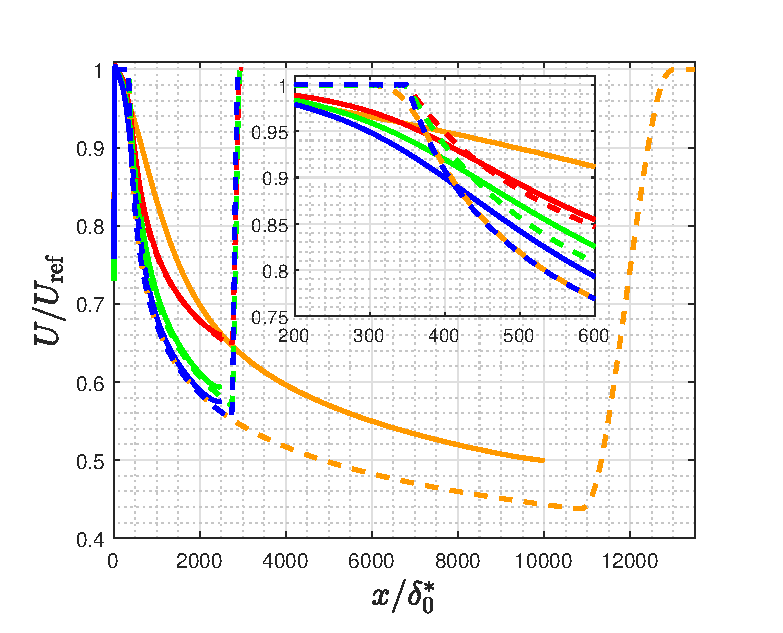
\includegraphics[width=0.6\textwidth]{fig1.eps}
  \caption{Streamwise evolution of (dashed) velocity at the top of the domain $U_{\rm top}(x)$ and (solid) velocity at the boundary-layer edge $U_e(x)$. Colors: (\protect\orangeline) b1.4; (\protect\redline) b1; (\protect\greenline) b2; (\protect\blueline) m16.}
%   Colors as in table \ref{tab:param}.}
\label{fig:U_BCs}
\end{figure}

 In figure \ref{fig:U_BCs} we show the streamwise evolution of $U_{\rm top}$ for the various cases under study, and it can be observed that this quantity is constant up to $x=350$, while it decays following a power law with different exponents $m$ for each APG \citep{bobke2017}. Note that the later rise of $U_{\rm top}$ is produced by the fringe.
 Since the BC is applied at the top of the domain and not at the edge of the BL, the velocity at the boundary-layer edge $U_e$ is not the same as $U_{\rm top}$, a fact that has been observed in multiple experiments and simulations of PG TBL and is still discussed in the scientific community as part of the problem of determining the edge of the TBL \citep{diagnostic_Vinuesa, d99_determination_2020}. The top boundary condition is far from the boundary-layer edge where the TBL  starts to develop, however, when the TBL starts to grow, this distance is reduced and the curves for $U_{\rm top}$ and $U_{e}$ come close to each other. This effect can be seen for the APGs by Bobke since the height of the domain was lower than in the larger b1.4 simulation.
 The fact that the the mean streamwise velocity $U$ exhibits a gradient ${\partial U}/{\partial y} \neq 0$ (which is a consequence of the streamwise PG) makes it harder to impose a specific velocity distribution at the edge of the BL, specially for the larger high-Reynolds simulations that require a taller computational domain for the TBL to grow. This effect could be reduced if the simulation could be performed in a domain with a variable height and not in a box of constant height.
 As a result of this effect, the imposed ZPG at $y=L_y$ is not perceived as a pure ZPG at the boundary layer edge, where the velocity instead of being constant, is slightly decaying as in an APG. As stated above, in the case where an auxiliary ZPG simulation gives the inflow, this effect of upstream influence of the APG will not be seen.
 The parameters for $U_{\rm top}$ are the same in the b1.4 and m16 cases, as can be observed in figure \ref{fig:U_BCs}, but the resulting $U_{e}$ is higher in the b1.4 than in the m16 case, which means that the decay of the velocity is not as steep in the former as in the latter and it will result in a smaller $\beta$. This shows that it is important to take into account the value of $L_y$ when setting the $U_{\rm top}(x)$ distribution to achieve a certain $U_{e}(x)$. 
 
Since we use a zero-spanwise vorticity as a BC, it is possible to rewrite the Reynolds-averaged Navier--Stokes (RANS) equations for the momentum in $x$ and $y$ in terms of the mean spanwise vorticity and its derivatives.
Being outside of the TBL means that the Reynolds stresses can be neglected if the turbulence is confined in the BL.
The first derivatives in $x$ and $y$ of $U$ and $V$ are present in the continuity equation and the mean spanwise vorticity $\Omega_z$. If those two equations are derived in $x$ and $y$ then it is possible to obtain relationships between the first derivatives of $\Omega_z$ with the second derivatives of $U$ and $V$ (present in the viscous terms of the RANS equations). Substituting the spanwise vorticity and its first derivatives in the convective and viscous terms we get:

\begin{equation}\label{eq:RANS_x_BC_OMEGA}
    U \frac {\partial U} {\partial x} + V \frac {\partial V} {\partial x} +
      \frac {1} {\rho} \frac {\partial P} {\partial x} = 
      \nu \left( \frac {\partial \Omega_z} {\partial y} \right) + V \Omega_z,
\end{equation}
\begin{equation}\label{eq:RANS_Y_BC_OMEGA}
    U \frac {\partial U} {\partial y} + V \frac {\partial V} {\partial y} +
      \frac {1} {\rho} \frac {\partial P} {\partial y} = 
      \nu \left( \frac {\partial \Omega_z} {\partial x} \right) + U \Omega_z,
\end{equation}
where $P$ is the pressure. In these equations we can see the effects of using a zero-spanwise vorticity or also making its derivatives zero. The convective terms on the left-hand side can be written as the gradient of a total pressure   $P_T / \rho = P/\rho + (U^2+V^2)/2$ caused by the effects of non-zero spanwise vorticity. Even if the spanwise vorticity is set to zero at the top of the domain, this does not guarantee that it will remain zero in all the domain outside of the TBL.
The spanwise vorticity outside of the BL is related to the curvature of $P_T$ outside of the BL due to the growth of the BL.
 
% \section{ Turbulence statistics at moderately-high Reynolds numbers} \label{sec:RS_peaks_and_exp}

The streamwise development of the different simulations as well as statistics in different wall-normal profiles are given in appendix \hyperlink{AppA}{A}, where similar conclusions as the ones observed in \cite{bobke2017} for near-equilibrium flows at lower Reynolds numbers are observed and extended to higher $\Rey$ numbers. 

In this section we will present the Reynolds stresses obtained at different streamwise positions since later in section \ref{sec:Spectra} they will be decomposed in their spectral components.

In figure \ref{fig:beta} the Clauser pressure-gradient parameter $\beta=(\delta^*/\tau_w)  (\partial P/\partial x)_{e} $ is shown for the nearly-constant-$\beta$ simulations by \cite{bobke2017}, the current simulation and data obtained in experiments \citep{MTL_expSANMIGUEL} for a similar range of $\Rey_{\tau}-\beta$. Here, $\Rey_{\tau}=u_{\tau}\delta_{99}/\nu$ is the Reynolds number based on friction velocity and $\delta_{99}$ is the $99\%$ boundary-layer thickness, which was calculated by means of the method proposed by \cite{diagnostic_Vinuesa}.

For the following figures, the $Re_{\tau}=500$ profiles (outside the ROI) will be considered to observe effects of different $\beta$, comparing b1.4 with the other near-equilibrium APG simulations at lower $\Rey$. Three additional profiles within the ROI, at $\Rey_{\tau}=\{500, 1000, 1500\}$, will be used to determine the effects of moderate APG at higher $\Rey$ through a comparison with the high-$\Rey$ ZPG. The mean velocity profiles of these cases are shown in figure~\ref{fig:meanU} from Appendix~\hyperlink{AppA}{A}.

\begin{figure}
\centering
% \includegraphics[width=0.6\textwidth]{Statistics/Integ_quant/beta_exp.eps}
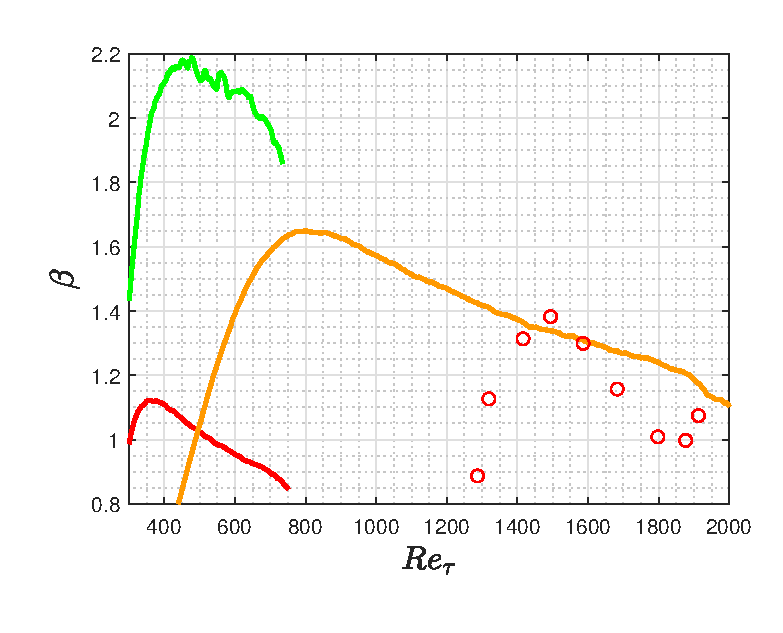
\includegraphics[width=0.6\textwidth]{fig2.eps}
  \caption{Evolution of the Clauser pressure-gradient parameter $\beta$ as a function of the friction Reynolds number $Re_{\tau}$ for three of the simulations Colors: (\protect\orangeline) b1.4; (\protect\redline) b1; (\protect\greenline) b2; (\protect\redcircle) experiments by \cite{MTL_expSANMIGUEL}.}
%   (colors as in table \ref{tab:param}) and the experiments by \cite{MTL_expSANMIGUEL} (represented by red circles).}
\label{fig:beta}
\end{figure}

The inner-scaled Reynolds stresses are shown in figure \ref{fig:RSinner}, and the corresponding profiles in outer scaling can be observed in appendix \hyperlink{AppA}{A}, figure \ref{fig:RSouter}. 
The most noticeable characteristic of these TBLs is that the wall affects each component of the Reynolds-stress (RS) tensor differently. The streamwise component has in general a larger value than the other terms, making it the leading term of the turbulent kinetic energy (TKE). Since at the wall the no-slip condition makes the velocities zero, the RSs also start from a zero level. In the viscous sub-layer the mean velocity gradually increases, together with the velocity fluctuations. 
In the near-wall region, {\it i.e.} at around $y^+\simeq 15$, the streamwise Reynolds stress exhibits the well-known inner peak, while the other fluctuating components are moderately affected by the strong TKE production in this region.

The APG significantly affects the inner peak of $\overline{u^2}^+$, and when this peak is scaled in outer units its magnitude decreases with APG magnitude (see figure \ref{fig:RSouter}a)). Interestingly, the near-wall fluctuations increase slightly with $\beta$ in the other velocity components when scaling in outer units (figure~\ref{fig:RSouter}), a result which is more prominent in the case of $\overline{w^2}$.

In the inner-scaled Reynolds stresses shown in figure \ref{fig:RSinner}, the influence of the APG can be observed in both $\overline{u^2}^+$ and $\overline{w^2}^+$, especially on the latter, from $y^+ \approx 2$ onward. However, the components containing the wall-normal velocity fluctuation are affected farther from the wall, starting at $y^+ \approx 10$ for $\Rey_{\tau}=500$ or even $y^+ \approx 20$ for higher $\Rey$. This behaviour supports the attached-eddy hypothesis on the differing contributions to the Reynolds stresses close to the wall \citep{Townsend_1976, deshpande_2021}, however, the trends are modified by the APG farther from the wall. 
The viscous scaling is appropriate for regions close to the wall, since it properly scales the mean streamwise velocity and the viscous length locates the inner peak of $\overline{u^2}^+$ at $y^+\approx 15$ (see figure \ref{fig:uupeaks_loc}a)). Furthermore, the friction velocity $u_{\tau}$ leads to more similar inner-peak magnitudes from different $\beta$ values than what is obtained using the outer velocity scale $U_{e}$. It is important to recall that the friction velocity is computed from ${\rm d}U / {\rm d} y$, which is the largest term of the near-wall TKE production also in APGs, closely connected with the formation of the inner peak in $\overline{u^2}^+$. The other components of the Reynolds stresses exhibit a better scaling using outer units even close to the wall, as shown in figure \ref{fig:RSouter} from Appendix A. 

 % Reynolds stress in inner units
\begin{figure}
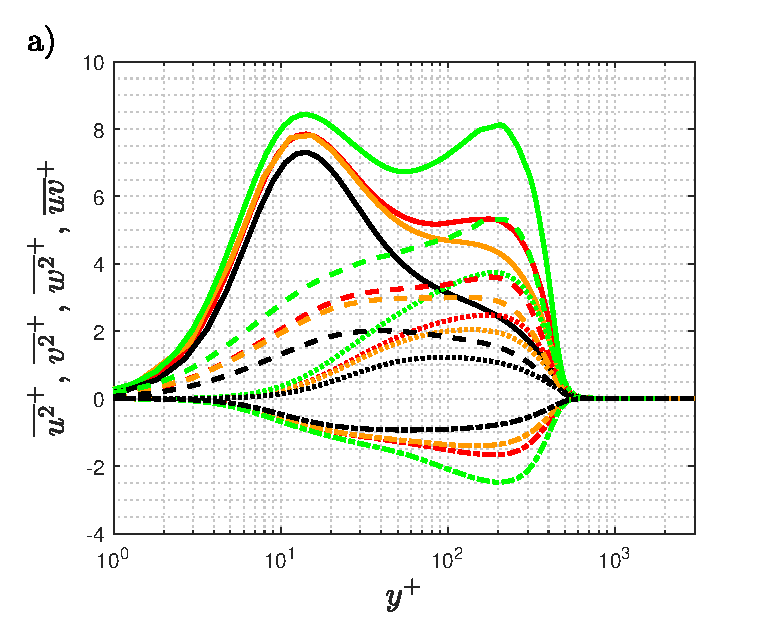
\includegraphics[width=0.49\textwidth]{fig3a.eps}
\includegraphics[width=0.49\textwidth]{fig3b.eps} \\
\includegraphics[width=0.49\textwidth]{fig3c.eps}
\includegraphics[width=0.49\textwidth]{fig3d.eps}
  \caption{Inner-scaled Reynolds stresses scaled with the friction velocity $u_{\tau}$ at various matched $Re_{\tau}$: a) $Re_{\tau}=500$ where $\beta(Re_{\tau})$ intersects for the simulations b1 and b1.4; b) $Re_{\tau}=1000$ ; c) $Re_{\tau}=1500$ ; d) $Re_{\tau}=2000$. Symbols: (\protect\blackline) $\overline{u^2}^+$; (\protect\blackdotted) $\overline{v^2}^+$; (\protect\blackdash) $\overline{w^2}^+$; (\protect\blackdashdot) $\overline{uv}^+$. Colors and symbols: (\protect\blackline) ZPG; (\protect\redline) b1; (\protect\orangeline) b1.4; (\protect\greenline) b2 as in table \ref{tab:param}.}
\label{fig:RSinner}
\end{figure}

To further study the impact of APG and $\Rey$ on the near-wall and outer peaks, it is important to have fine resolutions around $y^+=15$ and well-converged statistics in the outer region. 

Since the experimental database exhibits some noise, a curve-fit approach was considered around the inner and outer peaks of the streamwise RS to determine their locations, while a simple spline interpolation was employed for the numerical data.

In figure \ref{fig:uupeaks_loc} we show the streamwise evolution of the peak locations, where a clear influence of the APG is observed. Based on our results, an increasing APG magnitude leads to a larger wall-normal location of the inner peak $y^+_{IP}$, a phenomenon which is also observed for higher $\Rey$ at a given constant $\beta$. While for the ZPG case the near-wall-peak location reaches an asymptotic value of around $y^+ \simeq 15$ for $Re_{\tau} >2,000$, the trend in the b1.4 case is currently inconclusive.


\begin{figure}
\includegraphics[width=0.49\textwidth]{fig4a.eps}
\includegraphics[width=0.49\textwidth]{fig4b.eps} \\
\includegraphics[width=0.49\textwidth]{fig4c.eps}
\includegraphics[width=0.49\textwidth]{fig4d.eps}
\caption{Streamwise evolution of the wall-normal location of the inner and outer peaks of the streamwise Reynolds stress profiles. a) Inner-scaled position of the inner peak $y_{IP}^+$; b) and c) outer-peak location ($y_{OP}$) scaled with $\delta_{99}$ and $\delta^*$, respectively; d) inner-scaled outer-peak location $y^{+}_{OP}$. Colors: (\protect\blackline) ZPG; (\protect\orangeline) b1.4; (\protect\redline) b1; (\protect\greenline) b2; (\protect\blueline) m16; (\protect\magentaDiamond) $\beta=1$ DNS data from \cite{Kitsios2016}; (\protect\redcircle) experiments by \cite{MTL_expSANMIGUEL}; (\protect\blackSquare) experiments by \cite{skare_krogstad_1994}.}
\label{fig:uupeaks_loc}
\end{figure}
\begin{figure}
\includegraphics[width=0.49\textwidth]{fig5a.eps}
\includegraphics[width=0.49\textwidth]{fig5b.eps}\\
\includegraphics[width=0.49\textwidth]{fig5c.eps}
  \caption{Streamwise evolution of the magnitude of the inner and outer peaks of the streamwise Reynolds stress profiles. a) Inner-scaled magnitude of the inner peak $\overline{u^2}^+_{IP}$; b) and c) outer-peak magnitude ($\overline{u^2}_{OP}$) scaled in inner and outer units, respectively. Colors: (\protect\blackline) ZPG; (\protect\orangeline) b1.4; (\protect\redline) b1; (\protect\greenline) b2; (\protect\blueline) m16; (\protect\magentaDiamond) $\beta=1$ DNS data from \cite{Kitsios2016}; (\protect\redcircle) experiments by \cite{MTL_expSANMIGUEL}; (\protect\blackSquare) experiments by \cite{skare_krogstad_1994}. }
\label{fig:uupeaks_val}
\end{figure}

Figure \ref{fig:uupeaks_loc}b) shows the outer-peak location $y_{OP}$ of $\overline{u^2}$, scaled with the $99\%$ boundary-layer thickness, and our results indicate that the curve reaches a slightly decaying trend with $\Rey$ in the b1.4 case. 
Furthermore, comparison with the other cases indicates that the values of $y_{OP}/\delta_{99}$ are clearly affected by $\beta$, with stronger APGs leading to larger values of the outer-peak location. Note that although the value of $\beta$ is approximately the same in the b1 simulation and in the experiment, the former is at a much lower Reynolds number, and therefore this case is expected to perceive a more intense effect of the APG. This would explain that the outer-peak location is slightly farther away from the wall in the b1 case than in the experiment.
Figure \ref{fig:uupeaks_loc}c) shows the outer-peak location of $\overline{u^2}$ scaled with the displacement thickness $\delta^*$. The low-$\Rey$ simulations exhibit a similar slowly-growing trend for the various $\beta$ cases, with an average value of around $y_{OP}/\delta^* = 1.4$. The b1.4 case appears to reach an approximately constant state at higher $\Rey$, also around 1.4, a result consistent with that reported by \cite{Sanmiguel_PRF} for the experimental data (despite the noise present in the measurements).

The inner-scaled location of the outer peak present in the DNS by \cite{Kitsios2016} and the experiments by \cite{skare_krogstad_1994} are also shown in figure \ref{fig:uupeaks_loc}d). The outer-peak location of the $\beta=1$ DNS by \cite{Kitsios2016} continues the trend defined by the b1 LES at lower $\Rey$ and lies below the line of the b1.4 LES. The values of the near-equilibrium experimental data by \cite{skare_krogstad_1994} at a much higher $\Rey$ and $\beta \approx 20$ appear to be consistent with the linear trend of $y_{OP}^+$ established by the lower-$\Rey$ data.


The magnitudes of the inner ($\overline{u^2}_{IP}$) and outer ($\overline{u^2}_{OP}$) peaks of the streamwise RS are shown in the different panels of figure \ref{fig:uupeaks_val}.
In panel a) it is possible to see the Reynolds-number evolution of the inner-scaled inner peak ($\overline{u^2}_{IP}^+$) for the various APGs, as well as that of the ZPG TBL, which is well documented in the literature \citep{E-AmorZPG, Marusic_1997_ZPG}. While it is unclear what the behavior will be for the APG cases at higher $\Rey$, our data indicates that the inner-scaled near-wall peak increases with APG magnitude. The trend from the experiment exhibits more scatter, but it appears to be in qualitative agreement with that of the b1.4 case. Note that, although the inner peak in inner scaling increases with $\beta$, it actually decreases in outer scaling for stronger APGs, as can be observed in figure \ref{fig:RSouter}.
The outer-peak value increases with $\beta$ using inner scaling, as shown in figure \ref{fig:uupeaks_val}b), and also in outer scaling with $U_e$, as illustrated in figure \ref{fig:uupeaks_val}c). In both panels, the trends are approximately constant with $\Rey_{\tau}$, where $U_{e}$ yields a reasonably flat curve even at lower Reynolds numbers. 


In figure \ref{fig:uupeaks_val}b) the location of $\overline{u^2}^+$ for the $\beta=1$ DNS by \cite{Kitsios2017} and the b1 LES exhibit small differences probably associated with the different flow histories at low Reynolds numbers.
The experimental data by \cite{skare_krogstad_1994} exhibits a larger uncertainty and dispersion of the values, but an approximately-constant trend in $\overline{u^2}^+$ can be observed.

An unexpected trend is observed in figure \ref{fig:uupeaks_val}c) for the b1 simulation, a fact that could be attributed to the relatively low outer-peak values in this simulation.




%*********************************************************************************
% Experiments in MTL
%*********************************************************************************
\subsection{Comparison with experiments} 

The range of Reynolds numbers achieved in the b1.4 case allows for a direct comparison of the statistics with the experimental results by \cite{MTL_expSANMIGUEL}, where we selected two cases with matching $\beta$ and $\Rey_{\tau}$ conditions. As shown in  figure \ref{fig:beta}, the flow history of this database differs from that of the b1.4 case, a fact that will be taken into account when comparing the data.

\begin{figure}
\includegraphics[width=0.49\textwidth]{fig6a.eps}
\includegraphics[width=0.49\textwidth]{fig6b.eps}
\includegraphics[width=0.49\textwidth]{fig6c.eps}
\includegraphics[width=0.49\textwidth]{fig6d.eps}
\includegraphics[width=0.49\textwidth]{fig6e.eps}
\includegraphics[width=0.49\textwidth]{fig6f.eps}
\caption{Mean velocity (left column) and streamwise Reynolds stress (right column) scaled in viscous units as a function of the inner scaled wall-normal distance. The Reynolds numbers from top to bottom are $Re_{\tau}=\{1004, 1586, 2049\}$. The black solid line represents the ZPG by \cite{E-AmorZPG}, the orange line is the present b1.4 simulation and the red circles represent the experimental data by \cite{MTL_expSANMIGUEL}.}
\label{fig:experimentsMTL}
\end{figure}
%  Colors: (\protect\blackline) ZPG; (\protect\orangeline) b1.4; (\protect\redcircle) experiments by \cite{MTL_expSANMIGUEL}.

Three different profiles have been chosen in figure \ref{fig:experimentsMTL} to show the mean streamwise velocity and the streamwise Reynolds stress from the simulation and the experiment at matching $\Rey_{\tau}$. In the first row ($\Rey_{\tau}=1004$) the experimental TBL has a very low $\beta=0.3$, and it is very close to the ZPG, with small differences in the near-wall peak of $\overline{u^2}^+$ and a growing energy in the outer region of the TBL.
Here the simulation has a larger value of $\beta=1.6$, and it exhibits the most relevant features of APGs, including a prominent outer peak in $\overline{u^2}^+$.
In the middle row ($\Rey_{\tau}=1586$) the experimental data and the numerical simulation b1.4 exhibit the same  $\beta \simeq 1.4$. While the mean velocity profiles and the near-wall region of $\overline{u^2}^+$ is in good agreement in both cases, the simulation exhibits a larger fluctuation peak. This is due to the effect of flow history \citep{bobke2017, tanarro_2020}, but it is interesting to note that while the simulation is subjected to a mildly decaying $\beta(x)$ curve, the APG is rapidly increasing in the experiment. This implies that the smaller scales adapt more quickly to the local pressure gradient, while the larger scales require a longer streamwise distance.  
Finally, the higher Reynolds-number profile ($\Rey_{\tau}=2049$), where both TBLs have a value of $\beta \simeq 1.1$, exhibits a better collapse in both inner and outer peaks of $\overline{u^2}^+$, as well as in the mean velocity $U^+$.
This implies that, despite the different flow histories upstream, the two TBLs have been exposed to a similar PG magnitude for a sufficiently long streamwise distance such that their local turbulence features converge. Several profiles have been compared for $\Rey_{\tau}>1586$, and the best agreement between simulation and experiment is obtained for $\Rey_{\tau}=2049$. Upstream of this position the outer-peak value of the experimental data is still developing towards the value of the b1.4 case. The streamwise distance between the profiles at $\Rey_{\tau}=1586$ and 2049, which are subjected to a similar $\beta$ history, is around $11 \overline{\delta_{99}}$ for both simulation and experiment, where $\overline{\delta_{99}}$ is the average boundary-layer thickness between those profiles. A similar albeit lower of around $7\overline{\delta_{99}} $ was reported by \cite{bobke2017} for m16 simulation to converge towards b2 simulation at $\Rey_{\tau}=786$. One possible explanation for the longer distance reported here may be the higher Reynolds number, in which the large scales may require longer streamwise lengths to adapt to a particular pressure-gradient condition.

The APG in the simulation is achieved through a free-flow boundary condition, the turbulence is achieved through a tripping, therefore, the turbulence is confined inside the boundary layer with the Reynolds stresses being negligible outside of it. The experiments are performed inside a wind tunnel, the APG is imposed through changes in the geometry of the upper wall where another turbulent boundary layer develops. Even though the methods to establish the two APG TBLs are different, the results are remarkably similar. 
While the region outside of the boundary layer in the wind tunnel can be seen as the flow in the core of a channel where the mean $U$ does not exhibit a significant change, the free-flow APG condition has a negative $\partial{U}/\partial{y}$. This gradient, even if small, is present over a large distance in $y$, and when the mean profile is represented in a logarithmic scale it gives the impression of a drastic reduction of the mean velocity for $y>\delta_{99}$.
This comparison between numerical simulation and experiments shows a satisfactory collapse, and thus validates the high-Reynolds-number region of this numerical simulation.

% \section{Scaling considerations} \label{sec:Scalings}

One important question of wall-bounded turbulence research is to find a scaling that produces a collapse of statistical quantities such as the mean velocity or the Reynolds stresses in different parts of the TBL. Ideally, the scaling parameters should include the information of the forces/boundary conditions that could affect the flow, {\it i.e.} pressure gradients, temperature gradients, friction forces, flow history, etc.
Here we have an incompressible simulation of a flat-plate turbulent boundary layer where outside of the boundary layer there is an initial zero-pressure-gradient condition, which after a certain streamwise distance evolves into an adverse-pressure-gradient condition. The scaling parameters should include the effects of the friction at the wall ($\tau_w$), the pressure gradient, the Reynolds number and the flow history.
In the literature there are many studies of self-similarity (or self-preservation) focused on the equation of momentum conservation in $x$ under some ansatz and simplifications \citep{rotta1950theorie, Townsend_1956_structure, Castillo_2004, Kitsios2016, Gibis2019}. Most of those studies find parameters that should be kept constant to achieve self-similarity. Another question regarding self-similarity is whether it can be achieved across the whole boundary layer or whether the boundary layer can only be self-similar in different regions, with various scales.


%\subsection{Self-similarity analysis and scaling of the outer region}

Following the considerations about self-similarity in \citet{Gibis2019}, two sets of scalings will be considered in the outer region for the b1.4 and ZPG databases: the edge and the Zagarola--Smits (ZS) scalings as discussed below. The equilibrium character of the boundary layer will be assessed using the Rotta--Clauser pressure-gradient parameter $\beta$ together with the pressure-gradient boundary-layer growth parameter $\Lambda_{\rm inc}$ (\ref{eq:PG_Lambda}), for the chosen outer scalings.

\begin{equation} \label{eq:PG_Lambda}
    \Lambda_{\rm inc}=\frac{L_s}{\rho U_s^2 (\mathrm{d}L_s/\mathrm{d} x)} \frac{\mathrm{d}p}{\mathrm{d}x}.
\end{equation}
In the parameter $\Lambda_{\rm inc}$, $L_s$ represents the chosen length scale and $U_s$ the velocity length scale. If $L_s=\delta^*$ and $U_s=u_{\tau}$, then the difference with respect to the parameter $\beta$ will be given by the streamwise derivative of the length scale $\textrm{d} L_s/\textrm{d}x$, which contains some information of the flow history linking the local profile with the surrounding flow.
The different scalings with their respective velocity and length scales are summarized in table \ref{tab:Scaling_parameters}.
In figure \ref{fig:pg_parameters} the pressure-gradient parameter $\Lambda_{\rm inc}$ is shown for simulation b1.4 in the first row. While the edge scaling (left) shows a monotonically rising $\Lambda_{\rm inc}$ from the beginning, the ZS scaling (right) exhibits an initial peak, then a plateau, and finally a slowly-increasing region. On the other hand, $\beta$ (figure \ref{fig:beta}) exhibits a maximum and a slow monotonic decrease throughout the domain. Recalling that the ROI starts at $\Rey_{\tau}=800$, the range of variation of the PG parameter within the ROI is $[0.2, 0.25]$ for the edge scaling, $[3.2, 4]$ for the ZS scaling and $[1.65, 1.2]$ for $\beta$. The rates of variation of the PG parameters and $\textrm{d} L_s/\textrm{d}x$ over the ROI, although not constant, are relatively small, which is a requirement for similarity according to the various studies.

%*********************************************************************************
% Tobias Gibis JFM2019  "Self-Similar compressible turbulent...outer layer."
%*********************************************************************************
\begin{table}
  \begin{center}
\def~{\hphantom{0}}
    \begin{tabular}{ l c  c  l}
    Scaling         &     $L_s$        & $U_s$                          & Reference  \\[3pt]
    Rotta--Clauser  &  $U_e^+\delta^*$ & $u_{\tau}$                     & \cite{Clauser_1956}   \\
    Edge            &  $\delta^*$      & $U_e$                          & \cite{Kitsios2016}    \\
    Zagarola--Smits &  $\delta_{99}$   & $U_{e}(\delta^*/\delta_{99})$  & \cite{zagarola_smits} \\
    \end{tabular}
  \caption{Parameters for different scalings, where $L_s$ and $U_s$ correspond to the length and velocity scales, respectively.}
  \label{tab:Scaling_parameters}
  \end{center}
\end{table}

\begin{figure}
\includegraphics[width=0.49\textwidth]{fig7a.eps}
\includegraphics[width=0.49\textwidth]{fig7b.eps}
\includegraphics[width=0.49\textwidth]{fig7c.eps}
\includegraphics[width=0.49\textwidth]{fig7d.eps}
\caption{Different pressure-gradient parameters based on the self-similarity analysis for the outer layer performed in \citet{Gibis2019}. Left column represents the edge scaling, where $L_s=\delta^*$ and $U_s=U_e$. Right column shows the Zagarola--Smits scaling with $L_s=\delta_{99}$ and $U_s=U_{e}\delta^*/\delta_{99}$. A Savitzky--Golay filter has been applied to $\textrm{d} L_s/\textrm{d}x$ as in \cite{Gibis2019}. The black solid line represents the ZPG by \cite{E-AmorZPG} and the orange line is the present b1.4 simulation.}
\label{fig:pg_parameters}
\end{figure}

\begin{figure} 
\includegraphics[width=0.49\textwidth]{fig8a.eps}
\includegraphics[width=0.49\textwidth]{fig8b.eps}
\includegraphics[width=0.49\textwidth]{fig8c.eps}
\includegraphics[width=0.49\textwidth]{fig8d.eps}
\caption{(Top) Mean velocity defect and (bottom) streamwise Reynolds stress scaled with: edge (left) and Zagarola--Smits (right) scalings. Profiles from $Re_{\tau}=800$ to $Re_{\tau}=2000$. Lines in gray scale represent ZPG data \citep{E-AmorZPG}, increasing the Reynolds number from white to black. APG data from the b1.4 simulation increases Reynolds number from yellow to red.}
\label{fig:def_U_uu}
\end{figure}

In figure \ref{fig:def_U_uu} we use the edge and ZS scalings for the streamwise mean velocity defect and the streamwise RS for the profiles within the ROI.
The first observation is the common good agreement of both scalings from the logarithmic region all the way to the edge of the TBL in the ZPG.

Equation~(\ref{eq:defect_scaled_2}) shows the definition of $\delta^*$. For the ZS and edge scalings, the velocity and length scales are just a combination of the parameters present in equation~(\ref{eq:defect_scaled_2}) ($U_e$, $\delta^*$, $\delta_{99}$), therefore we can divide both sides by the term $U_e \delta^*$ and using the length and velocity scales in table \ref{tab:Scaling_parameters} it is possible to rewrite the integral in a common form (right-hand side of equation~(\ref{eq:defect_scaled_2})) for both ZS and edge scalings.

\begin{equation}\label{eq:defect_scaled_2}
    \int_{0}^{\delta_{99}} (U_e-U) \textrm{d} y = U_e \delta^*  \Rightarrow \int_{0}^{\delta_{99}/L_s} \frac{U_e-U}{U_s} \textrm{d}(y/L_s)=1. 
\end{equation}

Using this form we can directly relate the integral with the mean defect velocity curves in figure \ref{fig:def_U_uu}. 
 The value of the normalized integral of the mean velocity defect is the same for both scalings, where the integrands are the various curves and the only difference would be the upper limit of the integration. That upper limit in the ZS scaling does not change with the Reynolds number: it is 1 since $L_s=\delta_{99}$. The upper limit for the edge scaling is variable with Reynolds number because $L_s=\delta^*$. 
The functional form in the edge scaling fixes all the profiles to start from the same point, thus the differences between profiles increase from the wall. The functional form of the ZS scaling makes the profiles start from different values for each Reynolds number, and since the value of the integral is the same and the upper limit is also the same for all profiles, the differences are concentrated close to the wall, allowing for a better collapse in the outer region of the TBL.
This can be observed in figure \ref{fig:def_U_uu} (top right), where the ZS scaling exhibits a better collapse even in the overlap region. 
The edge scaling, figure \ref{fig:def_U_uu} (top left), exhibits a good collapse in the wake region, with differences in the overlap region.


We have previously discussed that the inner peak of $\overline{u^2}$ has a location $y^+ \simeq 15$. As shown in figure \ref{fig:def_U_uu} (bottom), and also in figure \ref{fig:uupeaks_loc}b) and c), the outer-peak location for the edge scaling is at $y/\delta^*=1.4$ and around $y/\delta_{99}=0.35$ for the ZS scaling.
While there is a better collapse in the outer region of the mean defect profiles using the ZS scaling, the $\overline{u^2}$ profiles collapse in the outer region when using the edge scaling.
Our results suggests that it is not possible to collapse the wall-normal profiles at all positions 
with a single length scale. In the mean flow, the inner region collapses in inner scaling and the outer region using the ZS scaling. Regarding the streamwise RS, the location of the near-wall peak slightly varies around $y^+\simeq 15$, it slowly grows with the Reynolds number and the slope is larger with higher $\beta$, whereas both the magnitude and location of the outer peak are fixed using the edge scaling. 
Since the inner and outer scales are related by $\Rey_{\tau}$, to achieve self-similarity throughout the whole profile would require that $\Rey_{\tau}$ remains constant in $x$, which is not the case even in the ZPG. 

\begin{figure}
\includegraphics[width=0.49\textwidth]{fig9a.eps}
\includegraphics[width=0.49\textwidth]{fig9b.eps}
\includegraphics[width=0.49\textwidth]{fig9c.eps}
\includegraphics[width=0.49\textwidth]{fig9d.eps}
\caption{Reynolds shear stress $\overline{uv}$ scaled with: edge (left) and Zagarola--Smits (right) scalings. The second row shows the effect of the evolution of the characteristic length scale $\textrm{d} L_s/\textrm{d}x$. Profiles from $Re_{\tau}=800$ to $Re_{\tau}=2000$. Lines in gray scale represent ZPG data \citep{E-AmorZPG}, increasing the Reynolds number from white to black. APG data from the b1.4 simulation increases Reynolds number from yellow to red.}
\label{fig:uv_scalings}
\end{figure}

In the next similarity analysis we consider the Reynolds shear stress, where in figure \ref{fig:uv_scalings} (top) we consider $U_s^2$, and in figure \ref{fig:uv_scalings} (bottom) we use $U_s^2 \textrm{d} L_s/\textrm{d}x$ as in \cite{Kitsios2016, Gibis2019}.
The edge scaling leads to a moderate collapse of the $\overline{uv}$ profiles in the outer region, although the collapse is not as good as the one observed for $\overline{u^2}$.
The additional term $\textrm{d} L_s/\textrm{d}x$ applied to the Reynolds shear stress, worsens the collapse for the APG in both scalings, while it improves the collapse for the ZPG in the edge scaling.

To summarize, the edge scaling yields a good scaling of the APG profiles in the outer region, and given the good collapse with viscous units close to the wall, it can be stated that the APG TBL is in near-equilibrium  \citep{Marusic_PoF_2010, bobke2017} conditions in the ROI.
The ZS scaling leads to a better collapse in the outer region of the mean defect profiles.

As observed in figure \ref{fig:kitsios_scalings},
comparing the first three profiles for both the ZPG and b1.4 cases a clear lack of collapse 
can be observed, and as discussed in figure \ref{fig:def_U_uu} the profiles only collapse in the inner or outer regions using the adequate scaling. We argue that any claims of self-similarity throughout the complete boundary layer may be based on limited regions of near-equilibrium conditions, which may hide the existing Reynolds-number trends. 
With these considerations we remark the importance of considering long regions of near equilibrium, where it is possible to clearly observe the trends in the inner and outer layers and to assess how the scales separate as the TBL develops. 

\begin{figure}
\includegraphics[width=0.32\textwidth]{fig10a.eps}
\includegraphics[width=0.32\textwidth]{fig10b.eps}
\includegraphics[width=0.32\textwidth]{fig10c.eps}
\includegraphics[width=0.32\textwidth]{fig10d.eps}
\includegraphics[width=0.32\textwidth]{fig10e.eps}
\caption{Mean streamwise velocity defect and Reynolds-stress tensor components $\overline{u^2}$, $\overline{v^2}$, $\overline{w^2}$, $\overline{uv}$ scaled using the edge scaling as in \cite{Kitsios2016}, and using the streamwise derivative of the length scale $\partial_x \delta^*$ in the case of $\overline{uv}$. The purple asterisks are used for the collapsed data by \cite{Kitsios2016}. The profiles have been taken at $\Rey_{\theta}=\{3500, 4150, 4800, 8200\}$, where the first three are in the same range as \cite{Kitsios2016} and the last at one is the highest $\Rey_{\theta}$ available in ZPG and b1.4 cases. Gray lines show the ZPG data growing in $\Rey$ from light to dark. The b1.4 lines show increase in Reynolds number from yellow to red.}
\label{fig:kitsios_scalings}
\end{figure}


 
% 
\section{Spectral analysis} \label{sec:Spectra}

The turbulent fluctuations are due to the interactions of a wide range of coherent structures of different sizes. Each of these structures will have a characteristic length and energy content. Depending on the approach used to decompose the energy content of the Reynolds-stress components in space/time we can have different types of representations.
The spectral analysis used here is based on a Fourier decomposition of the spanwise two-point correlations. The velocity correlation between two points along the spanwise direction provides an idea of lengths at which the fluctuations are highly correlated, and this gives an indication of the presence of a certain structure or pattern. In a multi-scale phenomenon such as turbulence at high Reynolds numbers, the two-point correlations will contain a mix of all the different scales and it will be difficult to obtain meaningful information from it. 
Since the spanwise direction is periodic, a Fourier decomposition of the two-point correlation is possible, and the result is a spectral decomposition of the energy content in different wavenumbers $k_z$ associated with their corresponding wavelengths $\lambda_z=2\pi/k_z$. 
In the next sections we show the premultiplied power-spectral density of the different Reynolds-stress components at matched values of $\Rey_{\tau}=500, 1000,1500,2000$. For reference, an additional contour has been added in gray for the maximum $\Rey_{\tau}=2386$ in the ZPG simulation.

%-------------------- Spec1D APG-ZPG ------------------------------------------------------------------------
\subsection{One-dimensional power-spectral density in z}

\begin{figure}
\includegraphics[width=0.49\textwidth]{fig11a.eps}
\includegraphics[width=0.49\textwidth]{fig11b.eps}
\includegraphics[width=0.49\textwidth]{fig11c.eps}
\includegraphics[width=0.49\textwidth]{fig11d.eps}
  \caption{Premultiplied spanwise power-spectral density $k_z |\phi_{uu}|$ scaled with the local maximum for the b1.4 and ZPG cases at matched $\Rey_{\tau}$. Contours taken at $10\%$, $50\%$, $90\%$ of the maximum value. Reference contour in gray colour: ZPG at $Re_{\tau}=2386$. Contours with (\protect\blackline) for ZPG and (\protect\orangeline) for b1.4. (Top-left) $Re_{\tau}=500$, (top-right) $Re_{\tau}=1000$, (bottom-left) $Re_{\tau}=1500$, (bottom-right) $Re_{\tau}=2000$.}
\label{fig:spec1DUU}
\end{figure}

The premultiplied power-spectral energy density of the streamwise velocity fluctuations is shown in figure \ref{fig:spec1DUU}; note that this corresponds to the highest energetic components of the turbulent kinetic energy.
This figure shows that the low-Reynolds-number case $Re_{\tau}=500$ exhibits similarities between the b1.4 and the ZPG TBLs. The APG starts to show its effects by lifting small scales with $\lambda_z^+ \approx 100$ from the wall to the outer region, and increasing the energy of the scales with $\lambda_z^+ \approx 400$ in the outer region. The near-wall spectral peak located at $y^+\approx 15$ and $\lambda_z^+ \approx 100$ remains similar in the APG and ZPG cases.
For increasing Reynolds number, the near-wall peak magnitude does not exhibit significant changes in the APG, but the maximum value shifts to the outer region at $\Rey_{\tau} \approx 700$, and is associated with scales of wavelength $\lambda_z=\delta_{99}$.
The inner and outer peaks are separated by a region of lower energy content, and the lowest-energy contour shows the characteristic rising of small scales by the APG in the outer region \citep{tanarro_2020, VINUESA2018}. The rest of the spectra exhibit similar features between the ZPG and the APG, except for a wider range of $\lambda_z^+$ across the boundary layer at the same $\Rey_{\tau}$, which is an effect of the footprint of large scales residing in the logarithmic region, similar to what was reported by \cite{Hoyas_PoF2006} for channel flows.
Note that at these Reynolds numbers the outer spectral peak of the APG has a magnitude similar to that of the near-wall peak in the ZPG.

\begin{figure}
\includegraphics[width=0.49\textwidth]{fig12a.eps}
\includegraphics[width=0.49\textwidth]{fig12b.eps}
\includegraphics[width=0.49\textwidth]{fig12c.eps}
\includegraphics[width=0.49\textwidth]{fig12d.eps}
  \caption{ Premultiplied cospectra $k_z |\phi_{uv}|$ scaled with the local maximum for the b1.4 and ZPG cases at matched $\Rey_{\tau}$. Contours taken at $10\%$, $50\%$, $90\%$ of the maximum value. Reference contour in gray colour: ZPG at $Re_{\tau}=2386$. Dashed black lines show the curve $y^+=0.27 \lambda_z^+$ as in \cite{giovanetti2016}, while the orange dashed lines represent $y^+=0.1 (\lambda_z^+)^{1.2}$, which is the ridge for the b1.4 case. Colors: (\protect\blackline) ZPG; (\protect\orangeline) b1.4. (Top-left) $Re_{\tau}=500$, (top-right) $Re_{\tau}=1000$, (bottom-left) $Re_{\tau}=1500$, (bottom-right) $Re_{\tau}=2000$.}
\label{fig:spec1DUV}
\end{figure}

In figure \ref{fig:spec1DUV} we show the premultiplied cospectra $k_z |\phi_{uv}|$ at the same matched $\Rey_{\tau}$ as in figure \ref{fig:spec1DUU}. 
At the lowest $\Rey_{\tau}$ the contours in the APG and the ZPG are similar, with the difference that the maximum value is in the outer region in the former ($y^+=120$ and $\lambda_z^+=307$) and closer to the wall ($y^+=26$ and $\lambda_z^+=109$) in the latter.
In the $10\%$ and $50\%$ contours, it is possible to see a small contribution of the small scales in the outer region compared to the ZPG contours.
At higher Reynolds numbers, the ZPG  develops a plateau of energy with contour levels following a straight line of slope $C$, which in a logarithmic plot corresponds to a power law of the form: $y^+=(\lambda_z^+)^C$.
This line connects the near-wall peak  with the outer region. Furthermore, the plateau indicates a progressive growth of the region containing this level of energy following the previous power law, which at $\Rey_{\tau}=1000$ develops an outer peak with a magnitude similar to that of the near-wall peak. Note that at higher Reynolds numbers the outer peak progressively rises over the magnitude of the near-wall peak.
The effect of the APG is to displace the near-wall energy to the outer region, which becomes dominant in the premultiplied cospectra of the Reynolds shear stress. At higher Reynolds numbers, the premultiplied cospectra exhibit a peak at $\lambda_z \simeq \delta_{99}$, which implies that this peak scales in outer units.
The constant $C$ which defines the slope of the black dashed lines in figure \ref{fig:spec1DUV} was reported to be $\approx 1$ by \cite{giovanetti2016}. The APG exhibits $10\%$ contours similar to those of the ZPG, indicating the presence of some energy in the near-wall region. If a line from the inner peak of the ZPG is drawn towards the APG peak in the outer region (orange dashed lines in figure \ref{fig:spec1DUV}), its slope is larger than that of the ZPG. If a self-similar hierarchy of motions in the log-layer is suggested by the black dashed line, in connection with the attached-eddy hypothesis \citep{Townsend_1976, deshpande_2021}, then the APG either rises the slope of that hierarchy of scales or follows the same hierarchy of motions as in the ZPG with an additional contribution in the outer region by small scales risen from the wall by the wall-normal convection of the APG and by the more energetic large scales.

The premultiplied spectra for the wall-normal fluctuations is shown in the first row of figure \ref{fig:spec1D_VV_WW}. It exhibits features similar to those of the cospectra of the Reynolds shear stress: small-scale energy in the outer region due to the APG and a different location of the maximum power-spectral density in the ZPG and the APG. While the ZPG exhibits an elongated $90\%$ contour around $\lambda_z^+ \approx 150$ at $y^+\approx 90$ for the different Reynolds numbers, the APG starts to stretch the peak at the lowest $\Rey_{\tau}=500$, and at $\Rey_{\tau}=1000$ the peak is located in the outer region with scales of the order of $\lambda_z \simeq \delta_{99}$.
In the ZPG the $10\%$ contours in the wall-normal spectra exhibit a shape similar to that of the $50\%$ contours in the cospectra. Approximating the $10\%$ contour by an ellipse, the major axis also follows a trend $y^+=(\lambda_z^+)^C$ with $C=1$, as in the cospectra. The $50\%$ contours also exhibit linear regions, but in the wall-normal spectra the slopes are different. This could still be related to a hierarchy of motions in the logarithmic layer, just indicating that the range of wall-normal scales grows with the wall-normal location and as before, the APG adds an extra contribution from the small and highly-energetic large scales in the outer part of the logarithmic layer. The $10\%$ contours of the APG follow the trend dictated by $\Rey_{\tau}$ and far from the trend marked by $y^+=(\lambda_z^+)^C$; for this reason, we have not included those linear trends.
As can be observed in the second row of figure \ref{fig:spec1D_VV_WW}, the spectra of the spanwise fluctuations exhibit effects similar to those shown in the wall-normal spectra in the first row for the ZPG and the APG. In particular we identify the small-scale contribution to the outer region and a stable $90\%$ contour for the ZPG expanding a long range of scales from $\lambda_z^+\approx 15$ to $\lambda_z^+\approx 70$ in a region between $y^+=15$ and $y^+=100$, which is inside the overlap region. This $90\%$ contour is displaced by the APG towards regions farther than $y^+=300$, already in the wake region. The $\lambda_z^+$ of this peak also scales with the Reynolds number.

\begin{figure}
\includegraphics[width=0.245\textwidth]{fig13a.eps}
\includegraphics[width=0.245\textwidth]{fig13b.eps}
\includegraphics[width=0.245\textwidth]{fig13c.eps}
\includegraphics[width=0.245\textwidth]{fig13d.eps}
\includegraphics[width=0.245\textwidth]{fig13e.eps}
\includegraphics[width=0.245\textwidth]{fig13f.eps}
\includegraphics[width=0.245\textwidth]{fig13g.eps}
\includegraphics[width=0.245\textwidth]{fig13h.eps}
  \caption{Premultiplied spanwise power-spectral density of $k_z |\phi_{vv}|$ (first row) and $k_z |\phi_{ww}|$ (second row) scaled with the local maximum for the b1.4 and ZPG cases at matched $\Rey_{\tau}$. Contours taken at $10\%$, $50\%$, $90\%$ of the maximum value. Reference contour in gray colour: ZPG at $Re_{\tau}=2386$. Contours with (\protect\blackline) for ZPG and (\protect\orangeline) for b1.4. From left to right: $Re_{\tau}=500$, $Re_{\tau}=1000$, $Re_{\tau}=1500$ and $Re_{\tau}=2000$.}
\label{fig:spec1D_VV_WW}
\end{figure}

%-----------------Spectra 2D------------------------------------------------------------
%-----uu--------------------

\subsection{Two-dimensional power-spectral density}

The two-dimensional power-spectral energy $E_{u_iu_j}(k_z,k_t,y)$ is obtained using temporal series of the velocities in all the spanwise grid points at selected streamwise and wall-normal positions. Once the mean in time and spanwise direction is substracted, the turbulent components are transformed to Fourier space in the spanwise wavenumbers. To obtain the power spectra in time, Welch's method is used with 8 independent subdivisions in time overlapped with 7 subdivisions for a total of 15 bins. The window function is a Hamming window.
The spectral energy is then divided by $\Delta k_z \Delta k_t$ to obtain the two-dimensional power-spectral density $\phi(k_z,k_t,y)$. As above, the figures used to illustrate the effects of the Reynolds number and the APG in the spectral-density content will be premultiplied, in this case, with the factor $k_z k_t$.
It has been verified that the addition of the spectral energy for all the wavenumbers in time yields the one-dimensional power-spectral energy in the spanwise direction $E_{u_i u_j}(k_z,y)$.


\subsubsection{Two-dimensional power-spectral density in the near-wall region}

The premultiplied power-spectral density in time and the spanwise direction $k_zk_t\phi(\lambda_z, \lambda_t)$ is first analysed at $y^+=15$, a wall-normal location which shows the characteristics of the near-wall peak of the streamwise RS and the production of TKE.
\begin{figure}
\includegraphics[width=0.24\textwidth]{fig14a.eps}
\includegraphics[width=0.24\textwidth]{fig14b.eps}
\includegraphics[width=0.24\textwidth]{fig14c.eps}
\includegraphics[width=0.24\textwidth]{fig14d.eps}
  \caption{Two-dimensional premultiplied power-spectral density $k_z k_t |\phi_{uu}|$ at $y^+=15$ scaled with the local maximum. Contours taken at $10\%$, $50\%$, $90\%$ of the maximum value. From left to right: $Re_{\tau}=500$, $Re_{\tau}=1000$, $Re_{\tau}=1500$ and $Re_{\tau}=2000$. The dashed blue line represents $\lambda_z^+ = 1.5\lambda_t^+$. Contours with (\protect\blackline) for ZPG and (\protect\orangeline) for b1.4.}
\label{fig:spec2D_uu_y15}
\end{figure}
For all the Reynolds numbers shown in figure \ref{fig:spec2D_uu_y15} there is a near-wall spectral peak with $\lambda_z^+ \approx 100$ and $\lambda_t^+$ of the order of 100. The blue dashed line represents $\lambda_z^+ = 1.5\lambda_t^+$, which describes the evolution with $\Rey$ of the ridge in the upper-right part of the spectrum. This ridge was documented by \cite{Hoyas_PoF2006} for channels, \cite{Sillero_2011}, for ZPG TBLs and \cite{tanarro_2020} for APG TBLs.
The APG does not significantly modify the spectrum around the near-wall peak and the local viscous length and time scales $l_{\tau}$ and $t_{\tau}$ lead to the collapse of the inner region for the three displayed contour levels.
Some extra energy is seen in the APG with the $50\%$ contours in the region with larger $\lambda_z^+$ and $\lambda_t^+$.
The biggest difference in the inner region is seen for the lowest Reynolds number, which is upstream of the ROI where near-equilibrium is achieved. At higher $\Rey_{\tau}$ values of 1000, 1500 and 2000, the spectra around the near-wall peak are identical for each simulation and grow closer to the ZPG contours. In figure \ref{fig:spec2D_uiuj_y15}, only the contours at $\Rey_{\tau}=500$ and 2000 are represented to show the differences in the region around the near-wall peak due to $\Rey_{\tau}=500$ being outside of the near-equilibrium region and to show the growth of the largest spatio-temporal scales.
\begin{figure}
\includegraphics[width=0.49\textwidth]{fig15a.eps}
\includegraphics[width=0.49\textwidth]{fig15b.eps}
\includegraphics[width=0.49\textwidth]{fig15c.eps}
\includegraphics[width=0.49\textwidth]{fig15d.eps}
  \caption{Evolution with the Reynolds number of the two-dimensional premultiplied power-spectral density in time and $z$ for the various Reynolds-stress components $k_z k_t |\phi_{u_iu_j}|$ at $y^+=15$ scaled with the local maximum. The panels show spectra of: a) $uu$, b) $vv$, c) $uv$, d) $ww$. Contours taken at $10\%$, $50\%$, $90\%$ of the maximum value. Solid lines for $Re_{\tau}=500$ and dotted lines for $Re_{\tau}=2000$. Colors: (\protect\blackline) for ZPG and (\protect\orangeline) for b1.4.}
\label{fig:spec2D_uiuj_y15}
\end{figure}

Surprisingly, the cospectra of the Reynolds shear stress shown in figure \ref{fig:spec2D_uiuj_y15}c) at $y^+=15$ does not exhibit significant differences between APG and ZPG nor with increasing $\Rey_{\tau}$. 
The behaviour of the streamwise and spanwise components is similar, since at higher Reynolds numbers the ZPG and the APG contours grow closer, both developing a region with larger values of $\lambda_z^+$, $\lambda_t^+$ with a higher energy content.
The wall-normal Reynolds stress does not develop a region with larger scales, and the lowest-density contour grows in the direction of smaller $\lambda_z^+$, $\lambda_t^+$.
The effect of $\Rey_{\tau}=500$ not being in near-equilibrium, as opposed to the higher-$\Rey_{\tau}$ profiles at 1000, 1500 and 2000 is reflected in a different slope of the $10\%$ contour in the lower region of the premultiplied spectra for the normal Reynolds stresses.


\subsubsection{Two-dimensional power-spectral density in the overlap region}
The analysis for the overlap region will be done at $y^+=150$ as in \cite{tanarro_2020} to compare the trends of $\lambda_{z}^+=f(\lambda_{t}^+)$ previously reported for channel flows in \cite{delAlamo_jfm_2004} and for boundary layers in \cite{chandran_jfm_rapids_2017}.
\begin{figure}
\includegraphics[width=0.31\textwidth]{fig16a.eps}
\includegraphics[width=0.31\textwidth]{fig16b.eps}
\includegraphics[width=0.31\textwidth]{fig16c.eps}
  \caption{Two-dimensional premultiplied power-spectral density $k_z k_t |\phi_{uu}|$ at $y^+=150$. The line styles solid, dashed, dash-dotted and dotted correspond to $Re_{\tau}=500, 1000, 1500$ and 2000 respectively. a) and b) are scaled with inner units, $u_{\tau}^2$, and show the contour levels 0.05 and 0.15 of the ZPG and b1.4 respectively. In a) and b) the red, blue and cyan lines are tangent to the contour level 0.15 of the ZPG. c) Represents both ZPG and b1.4 scaled with the local maximum marked as a black dot for ZPG and as a red dot for b1.4. The contours are taken at $10\%$ and $50\%$ of the maximum value. In c) the red, blue and cyan lines are moved to be tangent to the $10\%$ contour. Blue and cyan lines follow $\lambda_z^+ \propto (\lambda_t ^{+})^{0.5} $, while red line represents $\lambda_z^+ \propto \lambda_t^+$. Colors: (\protect\blackline) for ZPG and (\protect\orangeline) for b1.4.}
\label{fig:spec2Duu_yp150}
\end{figure}
In figure \ref{fig:spec2Duu_yp150} we show for $y^+=150$ the contour levels of energy 0.05 and 0.15 for the ZPG and for b1.4. At this wall-normal location and for the energy level 0.15, it was reported in \cite{tanarro_2020} a lower bound for small time and spanwise scales following $\lambda_z^+ \propto (\lambda_t ^{+})^{0.5} $ (blue-dashed line) and an upper bound composed by the red-dashed line ($\lambda_z^+ \propto \lambda_t^+$) for shorter time scales, as well as the cyan-dashed line for longer time scales (same slope as the blue-dashed line).
For the ZPG it is possible to see that for short scales there is a good collapse for different Reynolds numbers, and the lower limit (blue line) serves as a good approximation in spite of a small tendency with higher Reynolds numbers (at higher $\lambda_t^+$) to go towards wider scales for the same time scale.
The lower-energetic level 0.05 also presents a good collapse for the different Reynolds numbers, however, the slope of the trend (0.4) is slightly smaller than the one for energy level 0.15 (0.5).
The upper part of the contours are more curved than the lower part, therefore it is harder to come up with a linear trend in a logarithmic plot (potential law). The red line approximates a short region, $\lambda_t^+ \in (20, 60)$, while the cyan line seems to be a good approximation for the larger scales at higher Reynolds numbers.
The tangent lines to the energetic contour 0.15 of the ZPG are presented also in figure \ref{fig:spec2Duu_yp150}b) as a way to compare with the same energetic contour in b1.4. It is clear that in inner-scaling, the same energy contour is bigger in the APG than in the ZPG, expanding over shorter and larger scales. There is also a bigger dispersion of the contours due to the increasing Reynolds numbers.
The lower limits exhibit a slightly different slope than the blue line, however, with an increasing Reynolds number (dotted orange line) the trend is closer to the blue-dashed line. Since this is a fixed location at $y^+=150$ (see figure \ref{fig:spec1DUU}) at higher Reynolds numbers the differences between APG and ZPG are shifted towards higher wall-normal positions and larger $\lambda_z^+$ scales.
The red line ($\lambda_z^+ \propto \lambda_t^+$) appears to be a better approximation for the upper limit that will expand over a longer region , {\it i.e.} $\lambda_t^+ \in (10, 200)$ for $\Rey_{\tau}=2000$ compared to the case of the ZPG. The cyan line also seems to be a good approximation for the larger scales.
For $\Rey_{\tau}=2000$ the location of the local maximum for APG and ZPG is very similar. If the power-spectral density is non-dimensionalized by the local maximum as in figure \ref{fig:spec2Duu_yp150}c) the $10\%$ and $50\%$ contours of the ZPG and APG cases appears to collapse, except for some extra energy in the APG in the largest $\lambda_z^+$ and $\lambda_t^+$. The trends marked by the blue, red and cyan dashed lines are a better approximation at the higher $\Rey$.

For the lowest $\Rey_{\tau}$ in figure \ref{fig:spec2Duu_yp150_max} there is not a clear separation of scales. For each wall-normal plane, the local maximum of $k_z k_t |\phi_{uu}|$ evolves from the characteristic inner-peak wavelengths of $\lambda_z^+=100$ at $y^+=15$ towards wider scales $\lambda_z$ of the order of $\delta_{99}$ in the outer region.
At a higher Reynolds number as $\Rey_{\tau}=1000$ the location of the maxima in these premultiplied plots changes radically from scales $\lambda_z^+ \approx \mathcal{O} (100)$ and $\lambda_t^+ \approx \mathcal{O} (\lambda_z^+/2)$ to scales $\lambda_z \approx \mathcal{O}(\delta_{99})$. This change appears at $y^+\approx 23$ for b1.4 and $y^+\approx 40$ for the ZPG.  

At the position $y^+=150$ the peak of $k_z k_t |\phi_{uu}(k_z,k_t)|$ is already in scales $\lambda_z \approx \delta_{99}$ as it can be seen in figure \ref{fig:spec2Duu_yp150_max}c).
The other components of the Reynolds stress tensor are shown in figure \ref{fig:spec2Duiuj_150}.
As it was seen near the wall, at the lowest $\Rey_{\tau}=500$ (solid lines), the $10\%$ contour shows an additional content of energy for b1.4 in the smaller $\lambda_z^+$ scales with lower $\lambda_t^+$. 
The APG effects are manifested as a deviation of the local peak position and as it was seen near the wall, in the presence of small scales with shorter $\lambda_t^+$ in the wall-normal component, see figure \ref{fig:spec2Duiuj_150}b).
Previously, near the wall, the spectra containing wall-normal velocities in figure \ref{fig:spec2Duiuj_150}b) and c) was practically unaffected by an increase in the Reynolds number. On the other hand, in the outer region, both components develop larger spatio-temporal scales when the Reynolds number is increased. 
As observed in figure \ref{fig:spec2Duu_yp150_max}d) (and also in figure \ref{fig:spec2Duu_yp150}c)), the red-dashed line which approximates the contours for scales up to $\lambda_t^+ =100$ in the ZPG, reaches scales up to $\lambda_t^+ =200$ in the APG \citep{chandran_jfm_rapids_2017}.
The extra energy in the small scales with lower $\lambda_t^+$ is only seen in the lower $\Rey_{\tau}=500$ profiles of b1.4; for $\Rey_{\tau}=1000$, 1500 and 2000 that region is exhibits collapse.
In the 2D spectra shown in \cite{tanarro_2020}, the profiles were taken at different levels of the premultiplied spectral density scaled either in viscous or outer units. They reported that at the same contour level the APG effects extend over a wider range of scales compared to the ZPG contours at the same low $\Rey_{\tau}=305$. However, note that in their case the Reynolds number was low, the APG very strong and their boundary layers were not in near-equilibrium, exhibiting a rapid change in the $\beta(x)$ curve. Even if they achieved a value of $\beta$ larger than in the b1.4 simulation and an increase of the energy in the outer regions of the $\overline{u^2}^+$ TKE production profiles, the separation of scales in their study was not enough to observe the effects exhibited by the b1.4 simulation.

\begin{figure}
\includegraphics[width=0.49\textwidth]{fig17a.eps}
\includegraphics[width=0.49\textwidth]{fig17b.eps}
\includegraphics[width=0.49\textwidth]{fig17c.eps}
\includegraphics[width=0.49\textwidth]{fig17d.eps}
  \caption{Two-dimensional premultiplied power-spectral density $k_z k_t |\phi_{uu}|$ at $y^+=150$ scaled with the local maximum. Contours taken at $10\%$, $50\%$, $90\%$ of the maximum value. From left to right: a) $Re_{\tau}=500$, b) $Re_{\tau}=1000$, c) $Re_{\tau}=1500$ and d) $Re_{\tau}=2000$. The dashed blue and cyan lines represent $\lambda_z^+ \approx (\lambda_t^+)^{1/2}$, the dashed red line represents $\lambda_z^+ \approx \lambda_t^+$. The red and black dots mark the position of the local maximum for b1.4 and ZPG respectively. Colors: (\protect\blackline) for ZPG and (\protect\orangeline) for b1.4.}
\label{fig:spec2Duu_yp150_max}
\end{figure}

\begin{figure}
\includegraphics[width=0.49\textwidth]{fig18a.eps}
\includegraphics[width=0.49\textwidth]{fig18b.eps}
\includegraphics[width=0.49\textwidth]{fig18c.eps}
\includegraphics[width=0.49\textwidth]{fig18d.eps}
  \caption{Evolution with the Reynolds number of the two-dimensional premultiplied power-spectral density of the Reynolds-stress components $k_z k_t |\phi_{u_iu_j}|$ at $y^+=150$ scaled with the local maximum. The panels show spectra of: a) $uu$, b) $vv$, c) $uv$, d) $ww$. Contours taken at $10\%$, $50\%$, $90\%$ of the maximum value. Solid lines for $Re_{\tau}=500$ and dotted lines for $Re_{\tau}=2000$. Colors: (\protect\blackline) for ZPG and (\protect\orangeline) for b1.4.}
\label{fig:spec2Duiuj_150}
\end{figure}

 
% \section{Summary and conclusions} \label{sec:Conclusions}

A new well-resolved LES of a TBL developing on a flat plate subjected to an adverse pressure gradient is presented. The relevance of this simulation lies in the high Reynolds number we achieve starting from a laminar flow under similar conditions to those in experiments, and obtaining a long region where the TBL is in near-equilibrium. 
To the authors’ knowledge, this is the first TBL under approximately-constant APG magnitude  ($\beta\approx 1.4$) over a long near-equilibrium region up to $\Rey_{\theta}=8700$. The characteristics of this simulation have enabled a direct comparison with experimental data in a similar range of $\beta$ and $\Rey_{\tau}$, as well as the comparison with other near-equilibrium databases at lower Reynolds number as discussed below. 
The data obtained from the simulation consists of two-dimensional turbulence statistics for all the grid points in the $xy$ plane, together with time series and two-point correlations at 20 streamwise locations (containing all the spanwise grid points), with 10 of those profiles in the near-equilibrium ROI.

The turbulence statistics were compared with lower-Reynolds-number simulations of different APGs \citep{bobke2017}, with another high-Reynolds-number well-resolved LES of a ZPG \citep{E-AmorZPG} and also with high-Reynolds-number experiments \citep{MTL_expSANMIGUEL} with a similar $\beta(x)$ development. 
These comparisons highlight the need of more simulations with long near-equilibrium regions to be able to distinguish the effects of the APG and the effects of the Reynolds number. The near-equilibrium features have been analysed with the Rotta-Clauser pressure-gradient parameter $\beta$ and the parameter $\Lambda_{\rm inc}$ for different sets of velocity and length scales, {\it i.e.} the edge and the Zagarola--Smits scalings. Near-equilibrium conditions were obtained in the region from $\Rey_{\tau}=800$ to around 2000. 
The results were also compared to another constant-$\beta$ database \citep{Kitsios2016}, and we showed that any self-similarity analysis has to be performed along regions of near-equilibrium at high Reynolds numbers  to be able to study the collapse of the different regions in the TBL.
For the APGs under study here, the viscous scaling collapses the near-wall region for the streamwise mean velocity and although the magnitude of the near-wall peak of the streamwise RS increases in inner scaling, its location remains close to $y^+ \simeq 15$.
Furthermore, the outer scaling shows a good collapse of the outer region.

The large scales associated with the APG have an effect in the inner and outer regions, similarly to the large scales present in the flow at high Reynolds numbers in simpler geometries, such as channel flow \citep{Hoyas_PoF2006}. This was assessed for the various terms of the Reynolds-stress tensor using the spanwise one-dimensional power-spectral density and the two-dimensional power-spectral density in spanwise spatial scales and the temporal scales. 
This study shows that the displacement of small scales with $\lambda_z^+ \simeq 100$ from the inner to the outer region, documented in APGs at low Reynolds numbers by \cite{tanarro_2020, VINUESA2018}, is also observed in high-$\Rey$ APGs.
The present analysis at higher Reynolds numbers shows that there is an energization associated not only with the small scales but also with longer spatial and temporal scales in the streamwise and spanwise Reynolds stresses near the wall and in the overlap region.
The current database enables spatio-temporal analysis over a wide range of Reynolds numbers in near-equilibrium conditions due to the long near-equilibrium region at high $\Rey$. 
This type of high-quality APG TBL in near equilibrium is necessary to deepen our insight into the similar but different effects of Reynolds number and APG, and to further understand the role of flow history on the local features of wall-bounded turbulence 





\section{Introduction} \label{sec:Introduction}
%----------------------------------------------------
The study of boundary layers (BL) is the study of the behaviour of a fluid close to the boundary with another substance (solid, liquid or gas). We can use the knowledge of these boundary layers to predict the weather (systems atmosphere-Earth or atmosphere-sea) or even to manipulate a fluid for engineering purposes (production of electricity, mixing processes, transportation,...); note that most of these cases exhibit turbulent motions. In wall-bounded flows, as in the previous engineering examples, the optimization and control of the boundary layers is crucial for a good performance of the application under study. Some of the typical objectives are to reduce the drag in aeronautical surfaces, control the transition to turbulence or to avoid recirculation bubbles in ducts where achieving the maximum mass flow rate is important.

All the turbulent boundary layers (TBLs) in practical applications are subjected to streamwise pressure-gradients (PG), often with complex streamwise PG histories. These complicated variations of the PG can be divided into regions of adverse (APG), favourable (FPG) or zero pressure gradient (ZPG). The effects of PGs in wall-bounded turbulence are very diverse: a FPG drives the flow in a turbulent channel, while (if strong enough) it can produce relaminarization in flat-plate TBLs \citep{narasimha_sreenivasan_1973, FPG_araya2015}. On the opposite side, an APG can promote turbulence in a laminar BL and increase the turbulent fluctuations of a turbulent boundary layer; it can even produce flow separation, which is an undesirable phenomenon that reduces the performance of an aerodynamic device and can be dangerous if it happens on the wing of an airplane.
In wall-bounded flows the BL is affected by the wall geometry, the characteristics of the wall surface, the pressure-gradient distribution and the flow state beyond the BL. The effects on the wall will be seen as fluid-dynamic forces (lift and drag), but we could also be interested in effects produced after the solid, {\it i.e.} in the  the wake and its aeroacoustics properties (noise), or the wake instabilities that produce an increase in time between take-offs in airports.

Understanding the energy-transfer mechanisms within the TBL, and how they are affected by the pressure gradient, may lead to advancements in flow control and to new aerodynamic designs with higher performance.
The complexity of the problem has led to the definition of canonical TBLs in simple geometries, such as flat plates subjected to a ZPG or PG TBLs in equilibrium or near-equilibrium. 

It is important to discuss the concept of equilibrium and the effects of flow history. As discussed by \cite{Gibis2019} and \cite{Marusic_PoF_2010}, the term `equilibrium' has been used in different contexts in the literature. \cite{Clauser_1954_exp} denoted ``equilibrium profiles'' as those profiles of a boundary layer which develop maintaining a non-dimensional ``constant history'', defined as a constant ratio of the pressure-gradient and wall-shear forces, which can be written as the Clauser pressure-gradient parameter $\beta=\delta^{*}/\tau_w (\textrm{d}p/\textrm{d}x)$, where $\delta^{*}$ is the displacement thickness, $\tau_w$ is the shear stress at the wall, and $(\textrm{d}p/\textrm{d}x)$ is the pressure gradient. 
Later, the term `equilibrium' was used by \cite{rotta1962turbulent} and  \cite{townsend_1956_eqBL} as a synonym of self-preserving flow and in \cite{townsend_1961} it is used to refer to regions of the flow (`equilibrium layers') where there is a balance between rates of energy production and dissipation. In this context we will follow the same criterion as  \cite{Marusic_PoF_2010}, avoiding the use of equilibrium boundary layers and referring to near-equilibrium TBLs when the mean velocity-defect $U_{e}-U$ in the outer layer exhibits self-similarity (note that $U$ is the mean streamwise velocity and $U_e$ the velocity at the boundary-layer edge).

After these studies, many PG TBL experiments and simulations have been performed, with the aim of obtaining constant-$\beta$ distributions in order to obtain PG TBLs with a well-defined flow history, in this case with constant PG magnitude. 
If the equation of momentum in the streamwise direction is integrated across the boundary layer under several assumptions, then the momentum integral equation will relate the evolution of the momentum thickness $\theta$ with $\delta^*$ and $\beta$.

From he momentum integral equation, it is possible to derive the argument that $\beta$ must be constant to obtain self-similarity based on integral assumptions.

However, note that the ZPG TBL exhibits at least two different scalings: the near-wall region which scales properly using viscous units and the outer region, which does it with outer units (such as $\delta^*$ or the boundary layer thickness).

Therefore, the interest in establishing well-defined and close-to-constant $\beta$ distributions is not related to integral self-similarity arguments but lies in the fact that it is an integral parameter that quantifies the ratio between the pressure forces and the friction forces the boundary layer is subjected to throughout its evolution.

If this ratio had strong variations, especially at low Reynolds numbers, then it would be difficult to understand whether the observed phenomena are due to a local effect of the pressure gradient or the result of many different ratios of friction/pressure forces.

In this sense, a constant-$\beta$ configuration, in principle, allows to separate pressure-gradient and Reynolds-number effects, by comparing TBLs that only differ in the magnitude of the ratio between friction and pressure forces, since that ratio is maintained during the evolution of each BL, therefore, not mixing the contribution of flow history.

An example of constant $\beta$ are ZPG TBLs, which have been widely studied numerically e.g. by \cite{schlatter_orlu_2012, Sillero_2013pof} and experimentally by  \cite{bailey_2013_JFM, Orlu_Schlatter_exp2013, marusic_2015}. Regarding near-equilibrium APG simulations, it is important to highlight the direct numerical simulation (DNS) by \cite{Kitsios2016} with a constant $\beta=1$; the self-similar DNS TBL at the verge of separation ($\beta=39$) by \cite{Kitsios2017} or the well-resolved large-eddy simulation (LES) database comprising different PG intensities by \cite{bobke2017}. 
Some relevant experimental databases include the near-equilibrium APG TBLs by \cite{skare_krogstad_1994, MTL_expSANMIGUEL}, and the studies by \cite{MONTY2011} and \cite{harun_monty_2013}, where the flow history was not controlled.

For a complete study of PG TBLs it is necessary to obtain databases with near-equilibrium conditions extending over long streamwise regions so the effects of the PG and the Reynolds number can be clearly identified and studied. 
In this study we contribute towards that goal with a new well-resolved LES of incompressible and near-equilibrium APG TBL over a flat-plate with a nearly-constant value of $\beta \simeq 1.4$ over a large Reynolds-number range up to $Re_{\theta} \simeq 8,700$ (where $Re_{\theta}$ is the Reynolds number defined in terms of edge velocity and displacement thickness). The $\beta$ value is not constant along the streamwise development of the TBL, but its rate of reduction is small enough to be considered as nearly-constant, since the APG effects are larger for low Reynolds numbers and here we focus on a region of high Reynolds number. A comparison with experiments at similarly high $\Rey$ and $\beta$ values is carried out in this work, and even if the flow history of the experimental $\beta$ exhibits a larger variation, the profiles of the simulation and the experiment are in good agreement, indicating that these small deviations from a constant $\beta$ are not relevant in the region of high Reynolds number.

This is one of the largest simulations of a near-equilibrium APG TBL extending over a Reynolds-number range comparable to that of wind-tunnel experiments \citep{MTL_expSANMIGUEL}. 
Throughout this work, the results will be compared with the well-resolved LES ZPG TBL by \cite{EAmorZPG}, which exhibits a similar Reynolds-number range. These data-sets allow for a proper study of APG and Reynolds-number effects in the turbulent statistics as well as in the energetic scales involved in turbulence.

The article is organized as follows: in section \ref{sec:NumSetUp} the studied databases are presented, together with the numerical setup of the new simulation. 
The turbulent 2D statistics are compared with experimental data in section \ref{sec:RS_peaks_and_exp}.

Different scalings for the statistics will be considered in section \ref{sec:Scalings} and in order to understand the energetic scales as well as their distribution, the spectral analysis of the Reynolds stresses will be presented in section \ref{sec:Spectra}. 
In section \ref{sec:Conclusions} some conclusions on APG and Reynolds-number effects will be drawn, and an outlook will also be given. In appendix \hyperlink{AppA}{A} we include for the sake of completeness other turbulent statistics such as the streamwise evolution of integral parameters and the turbulent kinetic energy (TKE) budgets as well as the other 2D statistics in outer scaling that will serve as a support material to document the phenomena seen in the Reynolds stresses and spectra seen in previous sections.
Finally, appendix \hyperlink{AppB}{B} gives a breve description of the subgrid-scale model used in the present simulation.
 

\section{Numerical setup} \label{sec:NumSetUp}
The objective of the present simulation setup is to obtain a TBL developing under a moderate APG over a long region of near-equilibrium flow from low to high Reynolds numbers. To achieve a high-Reynolds-number simulation starting from a laminar flow we have taken as a reference the ZPG LES simulation by \cite{E-AmorZPG} based on \cite{Schlatter_etAl_LES_2010}, which on itself was validated using DNS by \cite{schlatter_orlu_2010}. The box size in the streamwise direction ($L_x$) was chosen to be identical to that of the ZPG simulation. The effect of an APG will increase the growth rate of the boundary layer together with the size of the energetic scales, and in order to account for this we increased the box size in the wall-normal ($L_y$) and spanwise directions ($L_z$) with respect to the values used by \cite{E-AmorZPG}, as can be observed in table \ref{tab:param}. Since the code used for the simulation, SIMSON \citep{simson_techrep}, uses Fourier modes in the streamwise direction, all the flow that has exited the domain through the top boundary due to the growth of the boundary layer, needs to enter again into the domain at the end of the box through a fringe region. 
The fringe length in the APG case will have to be longer than in the ZPG configuration, since a larger amount of flow leaves the domain in the former case and it will need to return through a negative wall-normal velocity component $V$, which will increase the Courant--Friedrichs--Lewy (CFL) number. The time step of the simulation was kept constant in order to perform Fourier analysis of the temporal series of the velocity components. Therefore, in order to have a constant time step that would not be too low and maintain a stable CFL, the fringe length had to be increased so the maximum $V$ was reduced in that region. It is important to mention that the CFL also depends on the spatial discretization, and since SIMSON uses Chebyshev polynomials in the wall-normal direction $y$, the wall-normal grid spacing ($\Delta y$) at the top boundary is too fine, if this spacing could be increased, then the CFL number would be reduced and it would be possible to use a shorter fringe with a higher $V$.

\subsection{Parameters of the simulation} \label{subsec:Param_sim}
The streamwise, wall-normal and spanwise coordinates $(x,y,z)$ and other lengths or distances are non-dimensionalized with the reference length $\delta^*_0$ (which is the displacement thickness of the inflow laminar boundary layer). In some parts of the text $\delta^*_0$ is not written for the sake of simplicity. That is also the case for the velocities, which are non-dimensionalized with the inflow free stream velocity $U_{\rm ref}$.
For all of the simulations in table \ref{tab:param} the same code (SIMSON) was employed, and the well-resolved LES is based on the same sub-grid-scale (SGS) model, ADM-RT, which stands for approximate deconvolution relaxation-term \citep{Schlatter_2004}, as discussed in more detail in appendix \hyperlink{AppB}{B}. In the present simulation, denoted by b1.4, we have used a new feature in the code: the implementation of message-passing interface (MPI) communication in single precision. In this version of the code, all the computations continue to be in double precision, but the time spent in communication between processors has been reduced by casting the data into single precision and reducing by half the amount of data to communicate. 

After selecting the box size we proceed to run the simulation with ZPG boundary conditions (BC) at a low resolution. The initial conditions and inflow profile are given by a laminar Blasius boundary layer with a displacement thickness $\delta^*_0$ such that $Re_{\delta_0^*}=450$. The flow is tripped to turbulence close to the inlet at $x/\delta^*_0=10$ using a volume forcing \citep{schlatter_orlu_2012}, which is the same method as in the other databases, and with this configuration we expect the transition to turbulence to be over at $Re_{\theta}\approx 600$ \citep{E-AmorZPG, schlatter_orlu_2012}. The TBL will develop to high Reynolds numbers over a long computational domain in a similar way as it is done in a wind-tunnel experiment. This is different from setting up an auxiliary ZPG simulation and using a recycle plane for the inflow as used in \cite{Kitsios2016, Kitsios2017, Gungor_DNS_2017}, since the APG BCs downstream would affect the initial ZPG, as can be seen in figure \ref{fig:U_BCs}. At the end of the domain a fringe region \citep{SIMSON_fringe} reduces the turbulence and yields the same laminar flow as the inflow in order to obtain the periodicity required by the Fourier discretization. 
One flow-through is defined as the time required by the flow to pass through the domain once; here the mean streamwise velocity is of the order of the unity, so we will approximate the time required by the flow to cover a distance $L_x$ to be equal to that distance. When the flow is fully turbulent after $\sim3$ flow-through times we proceeded to progressively change the APG BC to the desired distribution. In the final APG configuration, a fringe length of $1500 \delta^*_0$ is needed to keep the simulation stable.
The simulation was run for enough time for the statistics to converge \citep{vinuesa2016_mec} after excluding the initial transients due to the change of resolution. 
The statistics were averaged for over 8 and 4 eddy-turnover times (ETT) at the middle and the end of the region of interest respectively (note that the region of interest ends before the fringe). In APG TBLs the eddy-turnover time varies significantly with $x$, and it is calculated as: $ {\rm ETT}(x) = \Delta T  u_{\tau}(x) / \delta_{99}(x)$, with $\Delta T$ being the period of time used for averaging and $u_{\tau}(x)=\sqrt{(\tau_w / \rho)}$ the friction velocity.
We also collected time series containing 36,000 samples over the same period. 
The time step of the simulation is held constant at $\Delta t_{\rm step}=0.25$, which ensures that in viscous units the time step along the domain is $\Delta t_{\rm step}^+ \leq 0.35$. The statistics were sampled every 4 time steps in the region of interest, which corresponds to $\Delta t_{\rm stat}^+ \leq 0.5$.
The viscous scaling (denoted by the superscript `+') for velocity, length and time scales is:  $u_{\tau}$, $l_{\tau}=\nu/u_{\tau}$ and $t_{\tau}=l_{\tau}/u_{\tau}$.

In table \ref{tab:param} we show the box size, the collocation points using the 3/2 factor for de-aliasing ($m_x, m_y, m_z$) and the resolution of the various simulations. With the previous parameters we obtain the streamwise and spanwise resolution in viscous units ($\Delta x^+ , \Delta z^+$). The maximum separation of grid points in the wall-normal direction inside the boundary layer is shown in viscous units as $\Delta y_{\rm max}^+$, and it occurs close to the boundary-layer edge at the highest Reynolds numbers. In the new simulation b1.4, for $Re_{\tau}=500$, the number of grid points below $y^+=10$ is 6, below $y^+=1$ we have 2 and the distance of the first grid point from the wall is $\Delta y_w^+=0.3$. Since the viscous length scale $l_{\tau}$ increases with the streamwise position, the resolution in viscous units close to the wall will be better at higher Reynolds numbers: for $Re_{\tau}=800$ we have 7 grid points below $y^+=10$, 3 grid points below $y^+=1$ and $\Delta y_w^+=0.2$.
The color code that will be used along this work is shown in table \ref{tab:param}.

\begin{table}
  \begin{center}
  \fontsize{8.0pt}{10.25pt}\selectfont
  \addtolength{\tabcolsep}{-2pt}
\def~{\hphantom{0}}
    \begin{tabular}{ l r  r  r  r  r  r  r  r  r  r  r r}
    Case  & $L_x/\delta_0^*$ & $L_y/\delta_0^*$ & $L_z/\delta_0^*$ & $m_{x}$ & $m_{y}$ & $m_{z}$ & $\Delta x^{+}$ & $\Delta y_{\rm max}^{+}$ & $\Delta z^{+}$ & Colour & Reference \\[3pt]
    
    b1             &    3000   &   140   &    250  &    3072 &     301 &     576 &   21.8    & 8.4 &   9.7  & \redline     & Bobke (\citeyear{bobke2017}) \\
    b2             &    3000   &   180   &    320  &    3072 &     361 &     768 &   21.6    & 7.9 &   9.2  & \greenline   & Bobke (\citeyear{bobke2017}) \\
    m16            &    3000   &   180   &    220  &    3072 &     361 &     576 &   21.2    & 7.7 &   8.3  & \blueline    & Bobke (\citeyear{Bobke_2016}) \\

    ZPG            &   13500   &   400   &    540  &   13824 &     513 &    1152 &   22.6    & 19.6 &  10.9  & \blackline  & Eitel-Amor (\citeyear{E-AmorZPG}) \\
    b1.4           &   13500   &   800   &   1080  &   13824 &     301 &    1920 &   21.7    & 30.1 &  12.5  & \orangeline & Present study \\

    \end{tabular}
  \caption{Parameters of the simulations used in this paper. The inlet displacement thickness $\delta_0^*$ corresponds to the displacement thickness of a laminar flow for a Reynolds number $Re_{\delta_0^*}=450$. The box size is $(L_x/\delta_0^*, L_y/\delta_0^* , L_z/\delta_0^*)$  and $(m_x, m_y, m_z)$ are the number of collocation points including the $3/2$ factor for de-aliasing in the Fourier directions ($x$ and $z$). The spatial resolution in viscous units $(^+)$ of the streamwise and spanwise directions $\Delta x^{+}, \Delta z^{+}$, has been calculated using $(m_x, m_z)$ at the position $x/\delta_0^*=250$, which corresponds to a friction Reynolds number $Re_{\tau}\approx 210$ for all the simulations. The maximum viscous distance between grid points in the wall-normal direction inside the boundary layer is observed close to the boundary-layer edge and for the highest Reynolds number of each simulation. }
  \label{tab:param}
  \end{center}
\end{table}

The Reynolds-number and pressure-gradient ranges are shown in table \ref{tab:ROI},together with the region of interest (ROI) for each simulation. 
The ROI in the APG cases starts at the point where the maximum $\beta$ is achieved, while in the ZPG TBL, the starting point is taken at $Re_{\tau}=500$, which approximately corresponds to $Re_{\theta}\approx 1500$, where according to \cite{E-AmorZPG, schlatter_orlu_2012} the flow is independent of the inflow conditions and the tripping.
The last point of the ROI was chosen as the position where the skin-friction coefficient exhibits a clear tendency upwards due to the effects of the fringe; note that the large scales have not been affected yet.
In the ROI we observe a slowly-decaying positive $\beta$, where $\overline{\beta}$ is the average $\beta$ along the ROI. Note that this is not the accumulated $\overline{\beta}$ defined by \cite{Vinuesa_2017}, but a simple average instead. The standard deviation is $\sigma({\beta})$ and these quantities, together with the defect shape factor  $G=(H_{12}-1)/(H_{12}\sqrt{c_f/2})$, are given in table \ref{tab:ROI}. Note that $H_{12}$ and $c_f$ are the shape factor and the skin-friction coefficient, respectively. In the ROI of the b1.4 case, $G$ lies between 10.5 and 11.6, which is in agreement with the results reported by \cite{bobke2017}: 9.8 and 12.1 for the b1 and b2 cases, respectively.
\begin{table}
  \begin{center}
    \fontsize{8.0pt}{10.25pt}\selectfont
  \addtolength{\tabcolsep}{-2pt}
\def~{\hphantom{0}}
    \begin{tabular}{ l c  c  c  c  c  c c c}
    Case  & Range of $x/\delta_0^*$ & Range of $Re_{\tau}$ &  Range of $Re_{\theta}$ & Range of $\beta$ & $\overline{\beta}$ & $\sigma({\beta}) / \overline{\beta}$ & $G$ \\[3pt]
    
    b1             &     718 --  2101   &  350 -- 750   &  1320 -- 3080  & 1.12 -- 0.85 & 0.99 &  0.08 &    9.8 -- 10   \\
    b2             &    1148 --  2001   &  480 -- 730   &  2260 -- 3530  & 2.19 -- 1.86 & 2.06 &  0.04 &   12.1 -- 12.3 \\
    m16            &     823 --  2001   &  370 -- 740   &  1790 -- 3650  &  2.8 -- 1.9  & 2.42 &  0.11 &   12.5 -- 13.5 \\

    ZPG            &    1251 -- 11666   &  500 -- 2500  &  1430 -- 8200  &  $\simeq 0$  & $\simeq 0$ & $\simeq 0$ &   7.1 -- 7.2 \\
    b1.4           &    2455 --  8117   &  800 -- 1900  &  3700 -- 8700  & 1.65 -- 1.20 & 1.41 &  0.10 &   10.5 -- 11.6  \\
    \end{tabular}
  \caption{ Flow characteristics in the ROI for the various cases.}
  \label{tab:ROI}
  \end{center}
\end{table}


\subsection{Boundary conditions} \label{subsec:BC}

These simulations are statistically homogeneous in the spanwise direction $z$, therefore, they are statistically two-dimensional in the streamwise and wall-normal directions, and have periodic boundary conditions in the streamwise and spanwise directions. 
Since no cross-flow is present in the spanwise direction the only boundary condition (BC) is imposed by the periodicity. In the streamwise direction, the periodicity forces the outflow to be the same as the inflow, and this is achieved through a fringe region as mentioned above. 
The inflow is given by a Blasius boundary layer at $Re_{\delta^*_0}=450$.
At the bottom boundary of the computational domain there is a flat plate, the BCs of which are no-slip and no transpiration. 
The PG will be imposed at the top boundary of the domain with the free-stream boundary conditions discussed next.

\subsubsection{Free-stream boundary conditions}
Three conditions have to be imposed at the top of the domain:

\begin{equation} 
    \frac{\partial W}{\partial y}=0,
\label{eq:BC_dWdy}
\end{equation}

\begin{equation} 
    \Omega_z = \frac{\partial V}{\partial x} - \frac{\partial U}{\partial y}=0,
\label{eq:BC_Vort_z}
\end{equation}

\begin{equation}
    U_{\rm top}(x)= \left\{ \begin{array}{ll}
             U_{\rm ref}, &  x \leq x_z \\
             \\ U_{\rm ref}\left( 1 + \frac{x - x_{z}}{x_{b}} \right)^{-m}, & x > x_z.
             \end{array}
   \right.
\label{eq:BC_APG_U}
\end{equation}
The first one relates to the statistical homogeneity in $z$, through the derivative in the wall-normal direction of the spanwise mean velocity as shown in (\ref{eq:BC_dWdy}).
Homogeneity in $z$ implies that $W$ is statistically zero, therefore its wall-normal derivative should also be zero.
Homogeneity also implies that the mean derivatives in $z$ are statistically zero, a fact that has an implication in the mean streamwise vorticity, {\it i.e.}  $\Omega_x = \partial W/ \partial y - \partial V / \partial z = 0$.
This could be implemented in the simulation in multiple ways, but since the perturbations in the farfield are negligible in our case, the easiest way is to set $\partial \widetilde{w} / \partial y = 0$ for each time step, where ($\widetilde{ ~~ }$) denotes instantaneous quantities.
The second BC is zero spanwise vorticity, given by (\ref{eq:BC_Vort_z}) as in \cite{Kitsios2016, Abe_2019};
finally, the third BC will introduce the adverse pressure gradient through a decaying mean streamwise velocity $U_{\rm top}(x)$ using a power-law distribution. First, a constant velocity is used to provide an initial ZPG development and at $x=x_z=350$ the power law is applied as indicated in (\ref{eq:BC_APG_U}). At the end of the domain the fringe raises the velocity to the initial $U_{\rm ref}$ values. The power law was also used as in \cite{Bobke_2016}, based on the theoretical studies by \cite{Townsend_1956_structure} and \cite{mellor_gibson_1966} in order to obtain a near-equilibrium TBL.
The use of (\ref{eq:BC_APG_U}) together with a fringe region may produce instabilities in the code where the fringe region starts, which were damped by the LES filter. The parameters of the power law were chosen as in the m16 simulation \citep{Bobke_2016}, {\it i.e.},  $x_z=350$,  $x_b=60$ and $m=0.16$.



\begin{figure} 
\centering
    \includegraphics[width=0.6\textwidth]{fig1.eps}
  \caption{Streamwise evolution of (dashed) velocity at the top of the domain $U_{\rm top}(x)$ and (solid) velocity at the boundary-layer edge $U_e(x)$. Colors: (\protect\orangeline) b1.4; (\protect\redline) b1; (\protect\greenline) b2; (\protect\blueline) m16.}
%   Colors as in table \ref{tab:param}.}
\label{fig:U_BCs}
\end{figure}

 In figure \ref{fig:U_BCs} we show the streamwise evolution of $U_{\rm top}$ for the various cases under study, and it can be observed that this quantity is constant up to $x=350$, while it decays following a power law with different exponents $m$ for each APG \citep{bobke2017}. Note that the later rise of $U_{\rm top}$ is produced by the fringe.
 Since the BC is applied at the top of the domain and not at the edge of the BL, the velocity at the boundary-layer edge $U_e$ is not the same as $U_{\rm top}$, a fact that has been observed in multiple experiments and simulations of PG TBL and is still discussed in the scientific community as part of the problem of determining the edge of the TBL \citep{diagnostic_Vinuesa, d99_determination_2020}. The top boundary condition is far from the boundary-layer edge where the TBL  starts to develop, however, when the TBL starts to grow, this distance is reduced and the curves for $U_{\rm top}$ and $U_{e}$ come close to each other. This effect can be seen for the APGs by Bobke since the height of the domain was lower than in the larger b1.4 simulation.
 The fact that the the mean streamwise velocity $U$ exhibits a gradient ${\partial U}/{\partial y} \neq 0$ (which is a consequence of the streamwise PG) makes it harder to impose a specific velocity distribution at the edge of the BL, specially for the larger high-Reynolds simulations that require a taller computational domain for the TBL to grow. This effect could be reduced if the simulation could be performed in a domain with a variable height and not in a box of constant height.
 As a result of this effect, the imposed ZPG at $y=L_y$ is not perceived as a pure ZPG at the boundary layer edge, where the velocity instead of being constant, is slightly decaying as in an APG. As stated above, in the case where an auxiliary ZPG simulation gives the inflow, this effect of upstream influence of the APG will not be seen.
 The parameters for $U_{\rm top}$ are the same in the b1.4 and m16 cases, as can be observed in figure \ref{fig:U_BCs}, but the resulting $U_{e}$ is higher in the b1.4 than in the m16 case, which means that the decay of the velocity is not as steep in the former as in the latter and it will result in a smaller $\beta$. This shows that it is important to take into account the value of $L_y$ when setting the $U_{\rm top}(x)$ distribution to achieve a certain $U_{e}(x)$. 
 
Since we use a zero-spanwise vorticity as a BC, it is possible to rewrite the Reynolds-averaged Navier--Stokes (RANS) equations for the momentum in $x$ and $y$ in terms of the mean spanwise vorticity and its derivatives.
Being outside of the TBL means that the Reynolds stresses can be neglected if the turbulence is confined in the BL.
The first derivatives in $x$ and $y$ of $U$ and $V$ are present in the continuity equation and the mean spanwise vorticity $\Omega_z$. If those two equations are derived in $x$ and $y$ then it is possible to obtain relationships between the first derivatives of $\Omega_z$ with the second derivatives of $U$ and $V$ (present in the viscous terms of the RANS equations). Substituting the spanwise vorticity and its first derivatives in the convective and viscous terms we get:

\begin{equation}\label{eq:RANS_x_BC_OMEGA}
    U \frac {\partial U} {\partial x} + V \frac {\partial V} {\partial x} +
      \frac {1} {\rho} \frac {\partial P} {\partial x} = 
      \nu \left( \frac {\partial \Omega_z} {\partial y} \right) + V \Omega_z,
\end{equation}
\begin{equation}\label{eq:RANS_Y_BC_OMEGA}
    U \frac {\partial U} {\partial y} + V \frac {\partial V} {\partial y} +
      \frac {1} {\rho} \frac {\partial P} {\partial y} = 
      \nu \left( \frac {\partial \Omega_z} {\partial x} \right) + U \Omega_z,
\end{equation}
where $P$ is the pressure. In these equations we can see the effects of using a zero-spanwise vorticity or also making its derivatives zero. The convective terms on the left-hand side can be written as the gradient of a total pressure   $P_T / \rho = P/\rho + (U^2+V^2)/2$ caused by the effects of non-zero spanwise vorticity. Even if the spanwise vorticity is set to zero at the top of the domain, this does not guarantee that it will remain zero in all the domain outside of the TBL.
The spanwise vorticity outside of the BL is related to the curvature of $P_T$ outside of the BL due to the growth of the BL.
 
\section{ Turbulence statistics at moderately-high Reynolds numbers} \label{sec:RS_peaks_and_exp}

The streamwise development of the different simulations as well as statistics in different wall-normal profiles are given in appendix \hyperlink{AppA}{A}, where similar conclusions as the ones observed in \cite{bobke2017} for near-equilibrium flows at lower Reynolds numbers are observed and extended to higher $\Rey$ numbers. 

In this section we will present the Reynolds stresses obtained at different streamwise positions since later in section \ref{sec:Spectra} they will be decomposed in their spectral components.

In figure \ref{fig:beta} the Clauser pressure-gradient parameter $\beta=(\delta^*/\tau_w)  (\partial P/\partial x)_{e} $ is shown for the nearly-constant-$\beta$ simulations by \cite{bobke2017}, the current simulation and data obtained in experiments \citep{MTL_expSANMIGUEL} for a similar range of $\Rey_{\tau}-\beta$. Here, $\Rey_{\tau}=u_{\tau}\delta_{99}/\nu$ is the Reynolds number based on friction velocity and $\delta_{99}$ is the $99\%$ boundary-layer thickness, which was calculated by means of the method proposed by \cite{diagnostic_Vinuesa}.

For the following figures, the $Re_{\tau}=500$ profiles (outside the ROI) will be considered to observe effects of different $\beta$, comparing b1.4 with the other near-equilibrium APG simulations at lower $\Rey$. Three additional profiles within the ROI, at $\Rey_{\tau}=\{500, 1000, 1500\}$, will be used to determine the effects of moderate APG at higher $\Rey$ through a comparison with the high-$\Rey$ ZPG. The mean velocity profiles of these cases are shown in figure~\ref{fig:meanU} from Appendix~\hyperlink{AppA}{A}.

\begin{figure}
\centering
% \includegraphics[width=0.6\textwidth]{Statistics/Integ_quant/beta_exp.eps}
\includegraphics[width=0.6\textwidth]{fig2.eps}
  \caption{Evolution of the Clauser pressure-gradient parameter $\beta$ as a function of the friction Reynolds number $Re_{\tau}$ for three of the simulations Colors: (\protect\orangeline) b1.4; (\protect\redline) b1; (\protect\greenline) b2; (\protect\redcircle) experiments by \cite{MTL_expSANMIGUEL}.}
%   (colors as in table \ref{tab:param}) and the experiments by \cite{MTL_expSANMIGUEL} (represented by red circles).}
\label{fig:beta}
\end{figure}

The inner-scaled Reynolds stresses are shown in figure \ref{fig:RSinner}, and the corresponding profiles in outer scaling can be observed in appendix \hyperlink{AppA}{A}, figure \ref{fig:RSouter}. 
The most noticeable characteristic of these TBLs is that the wall affects each component of the Reynolds-stress (RS) tensor differently. The streamwise component has in general a larger value than the other terms, making it the leading term of the turbulent kinetic energy (TKE). Since at the wall the no-slip condition makes the velocities zero, the RSs also start from a zero level. In the viscous sub-layer the mean velocity gradually increases, together with the velocity fluctuations. 
In the near-wall region, {\it i.e.} at around $y^+\simeq 15$, the streamwise Reynolds stress exhibits the well-known inner peak, while the other fluctuating components are moderately affected by the strong TKE production in this region.

The APG significantly affects the inner peak of $\overline{u^2}^+$, and when this peak is scaled in outer units its magnitude decreases with APG magnitude (see figure \ref{fig:RSouter}a)). Interestingly, the near-wall fluctuations increase slightly with $\beta$ in the other velocity components when scaling in outer units (figure~\ref{fig:RSouter}), a result which is more prominent in the case of $\overline{w^2}$.

In the inner-scaled Reynolds stresses shown in figure \ref{fig:RSinner}, the influence of the APG can be observed in both $\overline{u^2}^+$ and $\overline{w^2}^+$, especially on the latter, from $y^+ \approx 2$ onward. However, the components containing the wall-normal velocity fluctuation are affected farther from the wall, starting at $y^+ \approx 10$ for $\Rey_{\tau}=500$ or even $y^+ \approx 20$ for higher $\Rey$. This behaviour supports the attached-eddy hypothesis on the differing contributions to the Reynolds stresses close to the wall \citep{Townsend_1976, deshpande_2021}, however, the trends are modified by the APG farther from the wall. 
The viscous scaling is appropriate for regions close to the wall, since it properly scales the mean streamwise velocity and the viscous length locates the inner peak of $\overline{u^2}^+$ at $y^+\approx 15$ (see figure \ref{fig:uupeaks_loc}a)). Furthermore, the friction velocity $u_{\tau}$ leads to more similar inner-peak magnitudes from different $\beta$ values than what is obtained using the outer velocity scale $U_{e}$. It is important to recall that the friction velocity is computed from ${\rm d}U / {\rm d} y$, which is the largest term of the near-wall TKE production also in APGs, closely connected with the formation of the inner peak in $\overline{u^2}^+$. The other components of the Reynolds stresses exhibit a better scaling using outer units even close to the wall, as shown in figure \ref{fig:RSouter} from Appendix A. 

 % Reynolds stress in inner units
\begin{figure}
\includegraphics[width=0.49\textwidth]{fig3a.eps}
\includegraphics[width=0.49\textwidth]{fig3b.eps} \\
\includegraphics[width=0.49\textwidth]{fig3c.eps}
\includegraphics[width=0.49\textwidth]{fig3d.eps}
  \caption{Inner-scaled Reynolds stresses scaled with the friction velocity $u_{\tau}$ at various matched $Re_{\tau}$: a) $Re_{\tau}=500$ where $\beta(Re_{\tau})$ intersects for the simulations b1 and b1.4; b) $Re_{\tau}=1000$ ; c) $Re_{\tau}=1500$ ; d) $Re_{\tau}=2000$. Symbols: (\protect\blackline) $\overline{u^2}^+$; (\protect\blackdotted) $\overline{v^2}^+$; (\protect\blackdash) $\overline{w^2}^+$; (\protect\blackdashdot) $\overline{uv}^+$. Colors and symbols: (\protect\blackline) ZPG; (\protect\redline) b1; (\protect\orangeline) b1.4; (\protect\greenline) b2 as in table \ref{tab:param}.}
\label{fig:RSinner}
\end{figure}

To further study the impact of APG and $\Rey$ on the near-wall and outer peaks, it is important to have fine resolutions around $y^+=15$ and well-converged statistics in the outer region. 

Since the experimental database exhibits some noise, a curve-fit approach was considered around the inner and outer peaks of the streamwise RS to determine their locations, while a simple spline interpolation was employed for the numerical data.

In figure \ref{fig:uupeaks_loc} we show the streamwise evolution of the peak locations, where a clear influence of the APG is observed. Based on our results, an increasing APG magnitude leads to a larger wall-normal location of the inner peak $y^+_{IP}$, a phenomenon which is also observed for higher $\Rey$ at a given constant $\beta$. While for the ZPG case the near-wall-peak location reaches an asymptotic value of around $y^+ \simeq 15$ for $Re_{\tau} >2,000$, the trend in the b1.4 case is currently inconclusive.


\begin{figure}
\includegraphics[width=0.49\textwidth]{fig4a.eps}
\includegraphics[width=0.49\textwidth]{fig4b.eps} \\
\includegraphics[width=0.49\textwidth]{fig4c.eps}
\includegraphics[width=0.49\textwidth]{fig4d.eps}
\caption{Streamwise evolution of the wall-normal location of the inner and outer peaks of the streamwise Reynolds stress profiles. a) Inner-scaled position of the inner peak $y_{IP}^+$; b) and c) outer-peak location ($y_{OP}$) scaled with $\delta_{99}$ and $\delta^*$, respectively; d) inner-scaled outer-peak location $y^{+}_{OP}$. Colors: (\protect\blackline) ZPG; (\protect\orangeline) b1.4; (\protect\redline) b1; (\protect\greenline) b2; (\protect\blueline) m16; (\protect\magentaDiamond) $\beta=1$ DNS data from \cite{Kitsios2016}; (\protect\redcircle) experiments by \cite{MTL_expSANMIGUEL}; (\protect\blackSquare) experiments by \cite{skare_krogstad_1994}.}
\label{fig:uupeaks_loc}
\end{figure}
\begin{figure}
\includegraphics[width=0.49\textwidth]{fig5a.eps}
\includegraphics[width=0.49\textwidth]{fig5b.eps}\\
\includegraphics[width=0.49\textwidth]{fig5c.eps}
  \caption{Streamwise evolution of the magnitude of the inner and outer peaks of the streamwise Reynolds stress profiles. a) Inner-scaled magnitude of the inner peak $\overline{u^2}^+_{IP}$; b) and c) outer-peak magnitude ($\overline{u^2}_{OP}$) scaled in inner and outer units, respectively. Colors: (\protect\blackline) ZPG; (\protect\orangeline) b1.4; (\protect\redline) b1; (\protect\greenline) b2; (\protect\blueline) m16; (\protect\magentaDiamond) $\beta=1$ DNS data from \cite{Kitsios2016}; (\protect\redcircle) experiments by \cite{MTL_expSANMIGUEL}; (\protect\blackSquare) experiments by \cite{skare_krogstad_1994}. }
\label{fig:uupeaks_val}
\end{figure}

Figure \ref{fig:uupeaks_loc}b) shows the outer-peak location $y_{OP}$ of $\overline{u^2}$, scaled with the $99\%$ boundary-layer thickness, and our results indicate that the curve reaches a slightly decaying trend with $\Rey$ in the b1.4 case. 
Furthermore, comparison with the other cases indicates that the values of $y_{OP}/\delta_{99}$ are clearly affected by $\beta$, with stronger APGs leading to larger values of the outer-peak location. Note that although the value of $\beta$ is approximately the same in the b1 simulation and in the experiment, the former is at a much lower Reynolds number, and therefore this case is expected to perceive a more intense effect of the APG. This would explain that the outer-peak location is slightly farther away from the wall in the b1 case than in the experiment.
Figure \ref{fig:uupeaks_loc}c) shows the outer-peak location of $\overline{u^2}$ scaled with the displacement thickness $\delta^*$. The low-$\Rey$ simulations exhibit a similar slowly-growing trend for the various $\beta$ cases, with an average value of around $y_{OP}/\delta^* = 1.4$. The b1.4 case appears to reach an approximately constant state at higher $\Rey$, also around 1.4, a result consistent with that reported by \cite{Sanmiguel_PRF} for the experimental data (despite the noise present in the measurements).

The inner-scaled location of the outer peak present in the DNS by \cite{Kitsios2016} and the experiments by \cite{skare_krogstad_1994} are also shown in figure \ref{fig:uupeaks_loc}d). The outer-peak location of the $\beta=1$ DNS by \cite{Kitsios2016} continues the trend defined by the b1 LES at lower $\Rey$ and lies below the line of the b1.4 LES. The values of the near-equilibrium experimental data by \cite{skare_krogstad_1994} at a much higher $\Rey$ and $\beta \approx 20$ appear to be consistent with the linear trend of $y_{OP}^+$ established by the lower-$\Rey$ data.


The magnitudes of the inner ($\overline{u^2}_{IP}$) and outer ($\overline{u^2}_{OP}$) peaks of the streamwise RS are shown in the different panels of figure \ref{fig:uupeaks_val}.
In panel a) it is possible to see the Reynolds-number evolution of the inner-scaled inner peak ($\overline{u^2}_{IP}^+$) for the various APGs, as well as that of the ZPG TBL, which is well documented in the literature \citep{E-AmorZPG, Marusic_1997_ZPG}. While it is unclear what the behavior will be for the APG cases at higher $\Rey$, our data indicates that the inner-scaled near-wall peak increases with APG magnitude. The trend from the experiment exhibits more scatter, but it appears to be in qualitative agreement with that of the b1.4 case. Note that, although the inner peak in inner scaling increases with $\beta$, it actually decreases in outer scaling for stronger APGs, as can be observed in figure \ref{fig:RSouter}.
The outer-peak value increases with $\beta$ using inner scaling, as shown in figure \ref{fig:uupeaks_val}b), and also in outer scaling with $U_e$, as illustrated in figure \ref{fig:uupeaks_val}c). In both panels, the trends are approximately constant with $\Rey_{\tau}$, where $U_{e}$ yields a reasonably flat curve even at lower Reynolds numbers. 


In figure \ref{fig:uupeaks_val}b) the location of $\overline{u^2}^+$ for the $\beta=1$ DNS by \cite{Kitsios2017} and the b1 LES exhibit small differences probably associated with the different flow histories at low Reynolds numbers.
The experimental data by \cite{skare_krogstad_1994} exhibits a larger uncertainty and dispersion of the values, but an approximately-constant trend in $\overline{u^2}^+$ can be observed.

An unexpected trend is observed in figure \ref{fig:uupeaks_val}c) for the b1 simulation, a fact that could be attributed to the relatively low outer-peak values in this simulation.




%*********************************************************************************
% Experiments in MTL
%*********************************************************************************
\subsection{Comparison with experiments} 

The range of Reynolds numbers achieved in the b1.4 case allows for a direct comparison of the statistics with the experimental results by \cite{MTL_expSANMIGUEL}, where we selected two cases with matching $\beta$ and $\Rey_{\tau}$ conditions. As shown in  figure \ref{fig:beta}, the flow history of this database differs from that of the b1.4 case, a fact that will be taken into account when comparing the data.

\begin{figure}
\includegraphics[width=0.49\textwidth]{fig6a.eps}
\includegraphics[width=0.49\textwidth]{fig6b.eps}
\includegraphics[width=0.49\textwidth]{fig6c.eps}
\includegraphics[width=0.49\textwidth]{fig6d.eps}
\includegraphics[width=0.49\textwidth]{fig6e.eps}
\includegraphics[width=0.49\textwidth]{fig6f.eps}
\caption{Mean velocity (left column) and streamwise Reynolds stress (right column) scaled in viscous units as a function of the inner scaled wall-normal distance. The Reynolds numbers from top to bottom are $Re_{\tau}=\{1004, 1586, 2049\}$. The black solid line represents the ZPG by \cite{E-AmorZPG}, the orange line is the present b1.4 simulation and the red circles represent the experimental data by \cite{MTL_expSANMIGUEL}.}
\label{fig:experimentsMTL}
\end{figure}
%  Colors: (\protect\blackline) ZPG; (\protect\orangeline) b1.4; (\protect\redcircle) experiments by \cite{MTL_expSANMIGUEL}.

Three different profiles have been chosen in figure \ref{fig:experimentsMTL} to show the mean streamwise velocity and the streamwise Reynolds stress from the simulation and the experiment at matching $\Rey_{\tau}$. In the first row ($\Rey_{\tau}=1004$) the experimental TBL has a very low $\beta=0.3$, and it is very close to the ZPG, with small differences in the near-wall peak of $\overline{u^2}^+$ and a growing energy in the outer region of the TBL.
Here the simulation has a larger value of $\beta=1.6$, and it exhibits the most relevant features of APGs, including a prominent outer peak in $\overline{u^2}^+$.
In the middle row ($\Rey_{\tau}=1586$) the experimental data and the numerical simulation b1.4 exhibit the same  $\beta \simeq 1.4$. While the mean velocity profiles and the near-wall region of $\overline{u^2}^+$ is in good agreement in both cases, the simulation exhibits a larger fluctuation peak. This is due to the effect of flow history \citep{bobke2017, tanarro_2020}, but it is interesting to note that while the simulation is subjected to a mildly decaying $\beta(x)$ curve, the APG is rapidly increasing in the experiment. This implies that the smaller scales adapt more quickly to the local pressure gradient, while the larger scales require a longer streamwise distance.  
Finally, the higher Reynolds-number profile ($\Rey_{\tau}=2049$), where both TBLs have a value of $\beta \simeq 1.1$, exhibits a better collapse in both inner and outer peaks of $\overline{u^2}^+$, as well as in the mean velocity $U^+$.
This implies that, despite the different flow histories upstream, the two TBLs have been exposed to a similar PG magnitude for a sufficiently long streamwise distance such that their local turbulence features converge. Several profiles have been compared for $\Rey_{\tau}>1586$, and the best agreement between simulation and experiment is obtained for $\Rey_{\tau}=2049$. Upstream of this position the outer-peak value of the experimental data is still developing towards the value of the b1.4 case. The streamwise distance between the profiles at $\Rey_{\tau}=1586$ and 2049, which are subjected to a similar $\beta$ history, is around $11 \overline{\delta_{99}}$ for both simulation and experiment, where $\overline{\delta_{99}}$ is the average boundary-layer thickness between those profiles. A similar albeit lower of around $7\overline{\delta_{99}} $ was reported by \cite{bobke2017} for m16 simulation to converge towards b2 simulation at $\Rey_{\tau}=786$. One possible explanation for the longer distance reported here may be the higher Reynolds number, in which the large scales may require longer streamwise lengths to adapt to a particular pressure-gradient condition.

The APG in the simulation is achieved through a free-flow boundary condition, the turbulence is achieved through a tripping, therefore, the turbulence is confined inside the boundary layer with the Reynolds stresses being negligible outside of it. The experiments are performed inside a wind tunnel, the APG is imposed through changes in the geometry of the upper wall where another turbulent boundary layer develops. Even though the methods to establish the two APG TBLs are different, the results are remarkably similar. 
While the region outside of the boundary layer in the wind tunnel can be seen as the flow in the core of a channel where the mean $U$ does not exhibit a significant change, the free-flow APG condition has a negative $\partial{U}/\partial{y}$. This gradient, even if small, is present over a large distance in $y$, and when the mean profile is represented in a logarithmic scale it gives the impression of a drastic reduction of the mean velocity for $y>\delta_{99}$.
This comparison between numerical simulation and experiments shows a satisfactory collapse, and thus validates the high-Reynolds-number region of this numerical simulation.

\section{Scaling considerations} \label{sec:Scalings}

One important question of wall-bounded turbulence research is to find a scaling that produces a collapse of statistical quantities such as the mean velocity or the Reynolds stresses in different parts of the TBL. Ideally, the scaling parameters should include the information of the forces/boundary conditions that could affect the flow, {\it i.e.} pressure gradients, temperature gradients, friction forces, flow history, etc.
Here we have an incompressible simulation of a flat-plate turbulent boundary layer where outside of the boundary layer there is an initial zero-pressure-gradient condition, which after a certain streamwise distance evolves into an adverse-pressure-gradient condition. The scaling parameters should include the effects of the friction at the wall ($\tau_w$), the pressure gradient, the Reynolds number and the flow history.
In the literature there are many studies of self-similarity (or self-preservation) focused on the equation of momentum conservation in $x$ under some ansatz and simplifications \citep{rotta1950theorie, Townsend_1956_structure, Castillo_2004, Kitsios2016, Gibis2019}. Most of those studies find parameters that should be kept constant to achieve self-similarity. Another question regarding self-similarity is whether it can be achieved across the whole boundary layer or whether the boundary layer can only be self-similar in different regions, with various scales.


%\subsection{Self-similarity analysis and scaling of the outer region}

Following the considerations about self-similarity in \citet{Gibis2019}, two sets of scalings will be considered in the outer region for the b1.4 and ZPG databases: the edge and the Zagarola--Smits (ZS) scalings as discussed below. The equilibrium character of the boundary layer will be assessed using the Rotta--Clauser pressure-gradient parameter $\beta$ together with the pressure-gradient boundary-layer growth parameter $\Lambda_{\rm inc}$ (\ref{eq:PG_Lambda}), for the chosen outer scalings.

\begin{equation} \label{eq:PG_Lambda}
    \Lambda_{\rm inc}=\frac{L_s}{\rho U_s^2 (\mathrm{d}L_s/\mathrm{d} x)} \frac{\mathrm{d}p}{\mathrm{d}x}.
\end{equation}
In the parameter $\Lambda_{\rm inc}$, $L_s$ represents the chosen length scale and $U_s$ the velocity length scale. If $L_s=\delta^*$ and $U_s=u_{\tau}$, then the difference with respect to the parameter $\beta$ will be given by the streamwise derivative of the length scale $\textrm{d} L_s/\textrm{d}x$, which contains some information of the flow history linking the local profile with the surrounding flow.
The different scalings with their respective velocity and length scales are summarized in table \ref{tab:Scaling_parameters}.
In figure \ref{fig:pg_parameters} the pressure-gradient parameter $\Lambda_{\rm inc}$ is shown for simulation b1.4 in the first row. While the edge scaling (left) shows a monotonically rising $\Lambda_{\rm inc}$ from the beginning, the ZS scaling (right) exhibits an initial peak, then a plateau, and finally a slowly-increasing region. On the other hand, $\beta$ (figure \ref{fig:beta}) exhibits a maximum and a slow monotonic decrease throughout the domain. Recalling that the ROI starts at $\Rey_{\tau}=800$, the range of variation of the PG parameter within the ROI is $[0.2, 0.25]$ for the edge scaling, $[3.2, 4]$ for the ZS scaling and $[1.65, 1.2]$ for $\beta$. The rates of variation of the PG parameters and $\textrm{d} L_s/\textrm{d}x$ over the ROI, although not constant, are relatively small, which is a requirement for similarity according to the various studies.

%*********************************************************************************
% Tobias Gibis JFM2019  "Self-Similar compressible turbulent...outer layer."
%*********************************************************************************
\begin{table}
  \begin{center}
\def~{\hphantom{0}}
    \begin{tabular}{ l c  c  l}
    Scaling         &     $L_s$        & $U_s$                          & Reference  \\[3pt]
    Rotta--Clauser  &  $U_e^+\delta^*$ & $u_{\tau}$                     & \cite{Clauser_1956}   \\
    Edge            &  $\delta^*$      & $U_e$                          & \cite{Kitsios2016}    \\
    Zagarola--Smits &  $\delta_{99}$   & $U_{e}(\delta^*/\delta_{99})$  & \cite{zagarola_smits} \\
    \end{tabular}
  \caption{Parameters for different scalings, where $L_s$ and $U_s$ correspond to the length and velocity scales, respectively.}
  \label{tab:Scaling_parameters}
  \end{center}
\end{table}

\begin{figure}
\includegraphics[width=0.49\textwidth]{fig7a.eps}
\includegraphics[width=0.49\textwidth]{fig7b.eps}
\includegraphics[width=0.49\textwidth]{fig7c.eps}
\includegraphics[width=0.49\textwidth]{fig7d.eps}
\caption{Different pressure-gradient parameters based on the self-similarity analysis for the outer layer performed in \citet{Gibis2019}. Left column represents the edge scaling, where $L_s=\delta^*$ and $U_s=U_e$. Right column shows the Zagarola--Smits scaling with $L_s=\delta_{99}$ and $U_s=U_{e}\delta^*/\delta_{99}$. A Savitzky--Golay filter has been applied to $\textrm{d} L_s/\textrm{d}x$ as in \cite{Gibis2019}. The black solid line represents the ZPG by \cite{E-AmorZPG} and the orange line is the present b1.4 simulation.}
\label{fig:pg_parameters}
\end{figure}

\begin{figure} 
\includegraphics[width=0.49\textwidth]{fig8a.eps}
\includegraphics[width=0.49\textwidth]{fig8b.eps}
\includegraphics[width=0.49\textwidth]{fig8c.eps}
\includegraphics[width=0.49\textwidth]{fig8d.eps}
\caption{(Top) Mean velocity defect and (bottom) streamwise Reynolds stress scaled with: edge (left) and Zagarola--Smits (right) scalings. Profiles from $Re_{\tau}=800$ to $Re_{\tau}=2000$. Lines in gray scale represent ZPG data \citep{E-AmorZPG}, increasing the Reynolds number from white to black. APG data from the b1.4 simulation increases Reynolds number from yellow to red.}
\label{fig:def_U_uu}
\end{figure}

In figure \ref{fig:def_U_uu} we use the edge and ZS scalings for the streamwise mean velocity defect and the streamwise RS for the profiles within the ROI.
The first observation is the common good agreement of both scalings from the logarithmic region all the way to the edge of the TBL in the ZPG.

Equation~(\ref{eq:defect_scaled_2}) shows the definition of $\delta^*$. For the ZS and edge scalings, the velocity and length scales are just a combination of the parameters present in equation~(\ref{eq:defect_scaled_2}) ($U_e$, $\delta^*$, $\delta_{99}$), therefore we can divide both sides by the term $U_e \delta^*$ and using the length and velocity scales in table \ref{tab:Scaling_parameters} it is possible to rewrite the integral in a common form (right-hand side of equation~(\ref{eq:defect_scaled_2})) for both ZS and edge scalings.

\begin{equation}\label{eq:defect_scaled_2}
    \int_{0}^{\delta_{99}} (U_e-U) \textrm{d} y = U_e \delta^*  \Rightarrow \int_{0}^{\delta_{99}/L_s} \frac{U_e-U}{U_s} \textrm{d}(y/L_s)=1. 
\end{equation}

Using this form we can directly relate the integral with the mean defect velocity curves in figure \ref{fig:def_U_uu}. 
 The value of the normalized integral of the mean velocity defect is the same for both scalings, where the integrands are the various curves and the only difference would be the upper limit of the integration. That upper limit in the ZS scaling does not change with the Reynolds number: it is 1 since $L_s=\delta_{99}$. The upper limit for the edge scaling is variable with Reynolds number because $L_s=\delta^*$. 
The functional form in the edge scaling fixes all the profiles to start from the same point, thus the differences between profiles increase from the wall. The functional form of the ZS scaling makes the profiles start from different values for each Reynolds number, and since the value of the integral is the same and the upper limit is also the same for all profiles, the differences are concentrated close to the wall, allowing for a better collapse in the outer region of the TBL.
This can be observed in figure \ref{fig:def_U_uu} (top right), where the ZS scaling exhibits a better collapse even in the overlap region. 
The edge scaling, figure \ref{fig:def_U_uu} (top left), exhibits a good collapse in the wake region, with differences in the overlap region.


We have previously discussed that the inner peak of $\overline{u^2}$ has a location $y^+ \simeq 15$. As shown in figure \ref{fig:def_U_uu} (bottom), and also in figure \ref{fig:uupeaks_loc}b) and c), the outer-peak location for the edge scaling is at $y/\delta^*=1.4$ and around $y/\delta_{99}=0.35$ for the ZS scaling.
While there is a better collapse in the outer region of the mean defect profiles using the ZS scaling, the $\overline{u^2}$ profiles collapse in the outer region when using the edge scaling.
Our results suggests that it is not possible to collapse the wall-normal profiles at all positions 
with a single length scale. In the mean flow, the inner region collapses in inner scaling and the outer region using the ZS scaling. Regarding the streamwise RS, the location of the near-wall peak slightly varies around $y^+\simeq 15$, it slowly grows with the Reynolds number and the slope is larger with higher $\beta$, whereas both the magnitude and location of the outer peak are fixed using the edge scaling. 
Since the inner and outer scales are related by $\Rey_{\tau}$, to achieve self-similarity throughout the whole profile would require that $\Rey_{\tau}$ remains constant in $x$, which is not the case even in the ZPG. 

\begin{figure}
\includegraphics[width=0.49\textwidth]{fig9a.eps}
\includegraphics[width=0.49\textwidth]{fig9b.eps}
\includegraphics[width=0.49\textwidth]{fig9c.eps}
\includegraphics[width=0.49\textwidth]{fig9d.eps}
\caption{Reynolds shear stress $\overline{uv}$ scaled with: edge (left) and Zagarola--Smits (right) scalings. The second row shows the effect of the evolution of the characteristic length scale $\textrm{d} L_s/\textrm{d}x$. Profiles from $Re_{\tau}=800$ to $Re_{\tau}=2000$. Lines in gray scale represent ZPG data \citep{E-AmorZPG}, increasing the Reynolds number from white to black. APG data from the b1.4 simulation increases Reynolds number from yellow to red.}
\label{fig:uv_scalings}
\end{figure}

In the next similarity analysis we consider the Reynolds shear stress, where in figure \ref{fig:uv_scalings} (top) we consider $U_s^2$, and in figure \ref{fig:uv_scalings} (bottom) we use $U_s^2 \textrm{d} L_s/\textrm{d}x$ as in \cite{Kitsios2016, Gibis2019}.
The edge scaling leads to a moderate collapse of the $\overline{uv}$ profiles in the outer region, although the collapse is not as good as the one observed for $\overline{u^2}$.
The additional term $\textrm{d} L_s/\textrm{d}x$ applied to the Reynolds shear stress, worsens the collapse for the APG in both scalings, while it improves the collapse for the ZPG in the edge scaling.

To summarize, the edge scaling yields a good scaling of the APG profiles in the outer region, and given the good collapse with viscous units close to the wall, it can be stated that the APG TBL is in near-equilibrium  \citep{Marusic_PoF_2010, bobke2017} conditions in the ROI.
The ZS scaling leads to a better collapse in the outer region of the mean defect profiles.

As observed in figure \ref{fig:kitsios_scalings},
comparing the first three profiles for both the ZPG and b1.4 cases a clear lack of collapse 
can be observed, and as discussed in figure \ref{fig:def_U_uu} the profiles only collapse in the inner or outer regions using the adequate scaling. We argue that any claims of self-similarity throughout the complete boundary layer may be based on limited regions of near-equilibrium conditions, which may hide the existing Reynolds-number trends. 
With these considerations we remark the importance of considering long regions of near equilibrium, where it is possible to clearly observe the trends in the inner and outer layers and to assess how the scales separate as the TBL develops. 

\begin{figure}
\includegraphics[width=0.32\textwidth]{fig10a.eps}
\includegraphics[width=0.32\textwidth]{fig10b.eps}
\includegraphics[width=0.32\textwidth]{fig10c.eps}
\includegraphics[width=0.32\textwidth]{fig10d.eps}
\includegraphics[width=0.32\textwidth]{fig10e.eps}
\caption{Mean streamwise velocity defect and Reynolds-stress tensor components $\overline{u^2}$, $\overline{v^2}$, $\overline{w^2}$, $\overline{uv}$ scaled using the edge scaling as in \cite{Kitsios2016}, and using the streamwise derivative of the length scale $\partial_x \delta^*$ in the case of $\overline{uv}$. The purple asterisks are used for the collapsed data by \cite{Kitsios2016}. The profiles have been taken at $\Rey_{\theta}=\{3500, 4150, 4800, 8200\}$, where the first three are in the same range as \cite{Kitsios2016} and the last at one is the highest $\Rey_{\theta}$ available in ZPG and b1.4 cases. Gray lines show the ZPG data growing in $\Rey$ from light to dark. The b1.4 lines show increase in Reynolds number from yellow to red.}
\label{fig:kitsios_scalings}
\end{figure}


 

\section{Spectral analysis} \label{sec:Spectra}

The turbulent fluctuations are due to the interactions of a wide range of coherent structures of different sizes. Each of these structures will have a characteristic length and energy content. Depending on the approach used to decompose the energy content of the Reynolds-stress components in space/time we can have different types of representations.
The spectral analysis used here is based on a Fourier decomposition of the spanwise two-point correlations. The velocity correlation between two points along the spanwise direction provides an idea of lengths at which the fluctuations are highly correlated, and this gives an indication of the presence of a certain structure or pattern. In a multi-scale phenomenon such as turbulence at high Reynolds numbers, the two-point correlations will contain a mix of all the different scales and it will be difficult to obtain meaningful information from it. 
Since the spanwise direction is periodic, a Fourier decomposition of the two-point correlation is possible, and the result is a spectral decomposition of the energy content in different wavenumbers $k_z$ associated with their corresponding wavelengths $\lambda_z=2\pi/k_z$. 
In the next sections we show the premultiplied power-spectral density of the different Reynolds-stress components at matched values of $\Rey_{\tau}=500, 1000,1500,2000$. For reference, an additional contour has been added in gray for the maximum $\Rey_{\tau}=2386$ in the ZPG simulation.

%-------------------- Spec1D APG-ZPG ------------------------------------------------------------------------
\subsection{One-dimensional power-spectral density in z}

\begin{figure}
\includegraphics[width=0.49\textwidth]{fig11a.eps}
\includegraphics[width=0.49\textwidth]{fig11b.eps}
\includegraphics[width=0.49\textwidth]{fig11c.eps}
\includegraphics[width=0.49\textwidth]{fig11d.eps}
  \caption{Premultiplied spanwise power-spectral density $k_z |\phi_{uu}|$ scaled with the local maximum for the b1.4 and ZPG cases at matched $\Rey_{\tau}$. Contours taken at $10\%$, $50\%$, $90\%$ of the maximum value. Reference contour in gray colour: ZPG at $Re_{\tau}=2386$. Contours with (\protect\blackline) for ZPG and (\protect\orangeline) for b1.4. (Top-left) $Re_{\tau}=500$, (top-right) $Re_{\tau}=1000$, (bottom-left) $Re_{\tau}=1500$, (bottom-right) $Re_{\tau}=2000$.}
\label{fig:spec1DUU}
\end{figure}

The premultiplied power-spectral energy density of the streamwise velocity fluctuations is shown in figure \ref{fig:spec1DUU}; note that this corresponds to the highest energetic components of the turbulent kinetic energy.
This figure shows that the low-Reynolds-number case $Re_{\tau}=500$ exhibits similarities between the b1.4 and the ZPG TBLs. The APG starts to show its effects by lifting small scales with $\lambda_z^+ \approx 100$ from the wall to the outer region, and increasing the energy of the scales with $\lambda_z^+ \approx 400$ in the outer region. The near-wall spectral peak located at $y^+\approx 15$ and $\lambda_z^+ \approx 100$ remains similar in the APG and ZPG cases.
For increasing Reynolds number, the near-wall peak magnitude does not exhibit significant changes in the APG, but the maximum value shifts to the outer region at $\Rey_{\tau} \approx 700$, and is associated with scales of wavelength $\lambda_z=\delta_{99}$.
The inner and outer peaks are separated by a region of lower energy content, and the lowest-energy contour shows the characteristic rising of small scales by the APG in the outer region \citep{tanarro_2020, VINUESA2018}. The rest of the spectra exhibit similar features between the ZPG and the APG, except for a wider range of $\lambda_z^+$ across the boundary layer at the same $\Rey_{\tau}$, which is an effect of the footprint of large scales residing in the logarithmic region, similar to what was reported by \cite{Hoyas_PoF2006} for channel flows.
Note that at these Reynolds numbers the outer spectral peak of the APG has a magnitude similar to that of the near-wall peak in the ZPG.

\begin{figure}
\includegraphics[width=0.49\textwidth]{fig12a.eps}
\includegraphics[width=0.49\textwidth]{fig12b.eps}
\includegraphics[width=0.49\textwidth]{fig12c.eps}
\includegraphics[width=0.49\textwidth]{fig12d.eps}
  \caption{ Premultiplied cospectra $k_z |\phi_{uv}|$ scaled with the local maximum for the b1.4 and ZPG cases at matched $\Rey_{\tau}$. Contours taken at $10\%$, $50\%$, $90\%$ of the maximum value. Reference contour in gray colour: ZPG at $Re_{\tau}=2386$. Dashed black lines show the curve $y^+=0.27 \lambda_z^+$ as in \cite{giovanetti2016}, while the orange dashed lines represent $y^+=0.1 (\lambda_z^+)^{1.2}$, which is the ridge for the b1.4 case. Colors: (\protect\blackline) ZPG; (\protect\orangeline) b1.4. (Top-left) $Re_{\tau}=500$, (top-right) $Re_{\tau}=1000$, (bottom-left) $Re_{\tau}=1500$, (bottom-right) $Re_{\tau}=2000$.}
\label{fig:spec1DUV}
\end{figure}

In figure \ref{fig:spec1DUV} we show the premultiplied cospectra $k_z |\phi_{uv}|$ at the same matched $\Rey_{\tau}$ as in figure \ref{fig:spec1DUU}. 
At the lowest $\Rey_{\tau}$ the contours in the APG and the ZPG are similar, with the difference that the maximum value is in the outer region in the former ($y^+=120$ and $\lambda_z^+=307$) and closer to the wall ($y^+=26$ and $\lambda_z^+=109$) in the latter.
In the $10\%$ and $50\%$ contours, it is possible to see a small contribution of the small scales in the outer region compared to the ZPG contours.
At higher Reynolds numbers, the ZPG  develops a plateau of energy with contour levels following a straight line of slope $C$, which in a logarithmic plot corresponds to a power law of the form: $y^+=(\lambda_z^+)^C$.
This line connects the near-wall peak  with the outer region. Furthermore, the plateau indicates a progressive growth of the region containing this level of energy following the previous power law, which at $\Rey_{\tau}=1000$ develops an outer peak with a magnitude similar to that of the near-wall peak. Note that at higher Reynolds numbers the outer peak progressively rises over the magnitude of the near-wall peak.
The effect of the APG is to displace the near-wall energy to the outer region, which becomes dominant in the premultiplied cospectra of the Reynolds shear stress. At higher Reynolds numbers, the premultiplied cospectra exhibit a peak at $\lambda_z \simeq \delta_{99}$, which implies that this peak scales in outer units.
The constant $C$ which defines the slope of the black dashed lines in figure \ref{fig:spec1DUV} was reported to be $\approx 1$ by \cite{giovanetti2016}. The APG exhibits $10\%$ contours similar to those of the ZPG, indicating the presence of some energy in the near-wall region. If a line from the inner peak of the ZPG is drawn towards the APG peak in the outer region (orange dashed lines in figure \ref{fig:spec1DUV}), its slope is larger than that of the ZPG. If a self-similar hierarchy of motions in the log-layer is suggested by the black dashed line, in connection with the attached-eddy hypothesis \citep{Townsend_1976, deshpande_2021}, then the APG either rises the slope of that hierarchy of scales or follows the same hierarchy of motions as in the ZPG with an additional contribution in the outer region by small scales risen from the wall by the wall-normal convection of the APG and by the more energetic large scales.

The premultiplied spectra for the wall-normal fluctuations is shown in the first row of figure \ref{fig:spec1D_VV_WW}. It exhibits features similar to those of the cospectra of the Reynolds shear stress: small-scale energy in the outer region due to the APG and a different location of the maximum power-spectral density in the ZPG and the APG. While the ZPG exhibits an elongated $90\%$ contour around $\lambda_z^+ \approx 150$ at $y^+\approx 90$ for the different Reynolds numbers, the APG starts to stretch the peak at the lowest $\Rey_{\tau}=500$, and at $\Rey_{\tau}=1000$ the peak is located in the outer region with scales of the order of $\lambda_z \simeq \delta_{99}$.
In the ZPG the $10\%$ contours in the wall-normal spectra exhibit a shape similar to that of the $50\%$ contours in the cospectra. Approximating the $10\%$ contour by an ellipse, the major axis also follows a trend $y^+=(\lambda_z^+)^C$ with $C=1$, as in the cospectra. The $50\%$ contours also exhibit linear regions, but in the wall-normal spectra the slopes are different. This could still be related to a hierarchy of motions in the logarithmic layer, just indicating that the range of wall-normal scales grows with the wall-normal location and as before, the APG adds an extra contribution from the small and highly-energetic large scales in the outer part of the logarithmic layer. The $10\%$ contours of the APG follow the trend dictated by $\Rey_{\tau}$ and far from the trend marked by $y^+=(\lambda_z^+)^C$; for this reason, we have not included those linear trends.
As can be observed in the second row of figure \ref{fig:spec1D_VV_WW}, the spectra of the spanwise fluctuations exhibit effects similar to those shown in the wall-normal spectra in the first row for the ZPG and the APG. In particular we identify the small-scale contribution to the outer region and a stable $90\%$ contour for the ZPG expanding a long range of scales from $\lambda_z^+\approx 15$ to $\lambda_z^+\approx 70$ in a region between $y^+=15$ and $y^+=100$, which is inside the overlap region. This $90\%$ contour is displaced by the APG towards regions farther than $y^+=300$, already in the wake region. The $\lambda_z^+$ of this peak also scales with the Reynolds number.

\begin{figure}
\includegraphics[width=0.245\textwidth]{fig13a.eps}
\includegraphics[width=0.245\textwidth]{fig13b.eps}
\includegraphics[width=0.245\textwidth]{fig13c.eps}
\includegraphics[width=0.245\textwidth]{fig13d.eps}
\includegraphics[width=0.245\textwidth]{fig13e.eps}
\includegraphics[width=0.245\textwidth]{fig13f.eps}
\includegraphics[width=0.245\textwidth]{fig13g.eps}
\includegraphics[width=0.245\textwidth]{fig13h.eps}
  \caption{Premultiplied spanwise power-spectral density of $k_z |\phi_{vv}|$ (first row) and $k_z |\phi_{ww}|$ (second row) scaled with the local maximum for the b1.4 and ZPG cases at matched $\Rey_{\tau}$. Contours taken at $10\%$, $50\%$, $90\%$ of the maximum value. Reference contour in gray colour: ZPG at $Re_{\tau}=2386$. Contours with (\protect\blackline) for ZPG and (\protect\orangeline) for b1.4. From left to right: $Re_{\tau}=500$, $Re_{\tau}=1000$, $Re_{\tau}=1500$ and $Re_{\tau}=2000$.}
\label{fig:spec1D_VV_WW}
\end{figure}

%-----------------Spectra 2D------------------------------------------------------------
%-----uu--------------------

\subsection{Two-dimensional power-spectral density}

The two-dimensional power-spectral energy $E_{u_iu_j}(k_z,k_t,y)$ is obtained using temporal series of the velocities in all the spanwise grid points at selected streamwise and wall-normal positions. Once the mean in time and spanwise direction is substracted, the turbulent components are transformed to Fourier space in the spanwise wavenumbers. To obtain the power spectra in time, Welch's method is used with 8 independent subdivisions in time overlapped with 7 subdivisions for a total of 15 bins. The window function is a Hamming window.
The spectral energy is then divided by $\Delta k_z \Delta k_t$ to obtain the two-dimensional power-spectral density $\phi(k_z,k_t,y)$. As above, the figures used to illustrate the effects of the Reynolds number and the APG in the spectral-density content will be premultiplied, in this case, with the factor $k_z k_t$.
It has been verified that the addition of the spectral energy for all the wavenumbers in time yields the one-dimensional power-spectral energy in the spanwise direction $E_{u_i u_j}(k_z,y)$.


\subsubsection{Two-dimensional power-spectral density in the near-wall region}

The premultiplied power-spectral density in time and the spanwise direction $k_zk_t\phi(\lambda_z, \lambda_t)$ is first analysed at $y^+=15$, a wall-normal location which shows the characteristics of the near-wall peak of the streamwise RS and the production of TKE.
\begin{figure}
\includegraphics[width=0.24\textwidth]{fig14a.eps}
\includegraphics[width=0.24\textwidth]{fig14b.eps}
\includegraphics[width=0.24\textwidth]{fig14c.eps}
\includegraphics[width=0.24\textwidth]{fig14d.eps}
  \caption{Two-dimensional premultiplied power-spectral density $k_z k_t |\phi_{uu}|$ at $y^+=15$ scaled with the local maximum. Contours taken at $10\%$, $50\%$, $90\%$ of the maximum value. From left to right: $Re_{\tau}=500$, $Re_{\tau}=1000$, $Re_{\tau}=1500$ and $Re_{\tau}=2000$. The dashed blue line represents $\lambda_z^+ = 1.5\lambda_t^+$. Contours with (\protect\blackline) for ZPG and (\protect\orangeline) for b1.4.}
\label{fig:spec2D_uu_y15}
\end{figure}
For all the Reynolds numbers shown in figure \ref{fig:spec2D_uu_y15} there is a near-wall spectral peak with $\lambda_z^+ \approx 100$ and $\lambda_t^+$ of the order of 100. The blue dashed line represents $\lambda_z^+ = 1.5\lambda_t^+$, which describes the evolution with $\Rey$ of the ridge in the upper-right part of the spectrum. This ridge was documented by \cite{Hoyas_PoF2006} for channels, \cite{Sillero_2011}, for ZPG TBLs and \cite{tanarro_2020} for APG TBLs.
The APG does not significantly modify the spectrum around the near-wall peak and the local viscous length and time scales $l_{\tau}$ and $t_{\tau}$ lead to the collapse of the inner region for the three displayed contour levels.
Some extra energy is seen in the APG with the $50\%$ contours in the region with larger $\lambda_z^+$ and $\lambda_t^+$.
The biggest difference in the inner region is seen for the lowest Reynolds number, which is upstream of the ROI where near-equilibrium is achieved. At higher $\Rey_{\tau}$ values of 1000, 1500 and 2000, the spectra around the near-wall peak are identical for each simulation and grow closer to the ZPG contours. In figure \ref{fig:spec2D_uiuj_y15}, only the contours at $\Rey_{\tau}=500$ and 2000 are represented to show the differences in the region around the near-wall peak due to $\Rey_{\tau}=500$ being outside of the near-equilibrium region and to show the growth of the largest spatio-temporal scales.
\begin{figure}
\includegraphics[width=0.49\textwidth]{fig15a.eps}
\includegraphics[width=0.49\textwidth]{fig15b.eps}
\includegraphics[width=0.49\textwidth]{fig15c.eps}
\includegraphics[width=0.49\textwidth]{fig15d.eps}
  \caption{Evolution with the Reynolds number of the two-dimensional premultiplied power-spectral density in time and $z$ for the various Reynolds-stress components $k_z k_t |\phi_{u_iu_j}|$ at $y^+=15$ scaled with the local maximum. The panels show spectra of: a) $uu$, b) $vv$, c) $uv$, d) $ww$. Contours taken at $10\%$, $50\%$, $90\%$ of the maximum value. Solid lines for $Re_{\tau}=500$ and dotted lines for $Re_{\tau}=2000$. Colors: (\protect\blackline) for ZPG and (\protect\orangeline) for b1.4.}
\label{fig:spec2D_uiuj_y15}
\end{figure}

Surprisingly, the cospectra of the Reynolds shear stress shown in figure \ref{fig:spec2D_uiuj_y15}c) at $y^+=15$ does not exhibit significant differences between APG and ZPG nor with increasing $\Rey_{\tau}$. 
The behaviour of the streamwise and spanwise components is similar, since at higher Reynolds numbers the ZPG and the APG contours grow closer, both developing a region with larger values of $\lambda_z^+$, $\lambda_t^+$ with a higher energy content.
The wall-normal Reynolds stress does not develop a region with larger scales, and the lowest-density contour grows in the direction of smaller $\lambda_z^+$, $\lambda_t^+$.
The effect of $\Rey_{\tau}=500$ not being in near-equilibrium, as opposed to the higher-$\Rey_{\tau}$ profiles at 1000, 1500 and 2000 is reflected in a different slope of the $10\%$ contour in the lower region of the premultiplied spectra for the normal Reynolds stresses.


\subsubsection{Two-dimensional power-spectral density in the overlap region}
The analysis for the overlap region will be done at $y^+=150$ as in \cite{tanarro_2020} to compare the trends of $\lambda_{z}^+=f(\lambda_{t}^+)$ previously reported for channel flows in \cite{delAlamo_jfm_2004} and for boundary layers in \cite{chandran_jfm_rapids_2017}.
\begin{figure}
\includegraphics[width=0.31\textwidth]{fig16a.eps}
\includegraphics[width=0.31\textwidth]{fig16b.eps}
\includegraphics[width=0.31\textwidth]{fig16c.eps}
  \caption{Two-dimensional premultiplied power-spectral density $k_z k_t |\phi_{uu}|$ at $y^+=150$. The line styles solid, dashed, dash-dotted and dotted correspond to $Re_{\tau}=500, 1000, 1500$ and 2000 respectively. a) and b) are scaled with inner units, $u_{\tau}^2$, and show the contour levels 0.05 and 0.15 of the ZPG and b1.4 respectively. In a) and b) the red, blue and cyan lines are tangent to the contour level 0.15 of the ZPG. c) Represents both ZPG and b1.4 scaled with the local maximum marked as a black dot for ZPG and as a red dot for b1.4. The contours are taken at $10\%$ and $50\%$ of the maximum value. In c) the red, blue and cyan lines are moved to be tangent to the $10\%$ contour. Blue and cyan lines follow $\lambda_z^+ \propto (\lambda_t ^{+})^{0.5} $, while red line represents $\lambda_z^+ \propto \lambda_t^+$. Colors: (\protect\blackline) for ZPG and (\protect\orangeline) for b1.4.}
\label{fig:spec2Duu_yp150}
\end{figure}
In figure \ref{fig:spec2Duu_yp150} we show for $y^+=150$ the contour levels of energy 0.05 and 0.15 for the ZPG and for b1.4. At this wall-normal location and for the energy level 0.15, it was reported in \cite{tanarro_2020} a lower bound for small time and spanwise scales following $\lambda_z^+ \propto (\lambda_t ^{+})^{0.5} $ (blue-dashed line) and an upper bound composed by the red-dashed line ($\lambda_z^+ \propto \lambda_t^+$) for shorter time scales, as well as the cyan-dashed line for longer time scales (same slope as the blue-dashed line).
For the ZPG it is possible to see that for short scales there is a good collapse for different Reynolds numbers, and the lower limit (blue line) serves as a good approximation in spite of a small tendency with higher Reynolds numbers (at higher $\lambda_t^+$) to go towards wider scales for the same time scale.
The lower-energetic level 0.05 also presents a good collapse for the different Reynolds numbers, however, the slope of the trend (0.4) is slightly smaller than the one for energy level 0.15 (0.5).
The upper part of the contours are more curved than the lower part, therefore it is harder to come up with a linear trend in a logarithmic plot (potential law). The red line approximates a short region, $\lambda_t^+ \in (20, 60)$, while the cyan line seems to be a good approximation for the larger scales at higher Reynolds numbers.
The tangent lines to the energetic contour 0.15 of the ZPG are presented also in figure \ref{fig:spec2Duu_yp150}b) as a way to compare with the same energetic contour in b1.4. It is clear that in inner-scaling, the same energy contour is bigger in the APG than in the ZPG, expanding over shorter and larger scales. There is also a bigger dispersion of the contours due to the increasing Reynolds numbers.
The lower limits exhibit a slightly different slope than the blue line, however, with an increasing Reynolds number (dotted orange line) the trend is closer to the blue-dashed line. Since this is a fixed location at $y^+=150$ (see figure \ref{fig:spec1DUU}) at higher Reynolds numbers the differences between APG and ZPG are shifted towards higher wall-normal positions and larger $\lambda_z^+$ scales.
The red line ($\lambda_z^+ \propto \lambda_t^+$) appears to be a better approximation for the upper limit that will expand over a longer region , {\it i.e.} $\lambda_t^+ \in (10, 200)$ for $\Rey_{\tau}=2000$ compared to the case of the ZPG. The cyan line also seems to be a good approximation for the larger scales.
For $\Rey_{\tau}=2000$ the location of the local maximum for APG and ZPG is very similar. If the power-spectral density is non-dimensionalized by the local maximum as in figure \ref{fig:spec2Duu_yp150}c) the $10\%$ and $50\%$ contours of the ZPG and APG cases appears to collapse, except for some extra energy in the APG in the largest $\lambda_z^+$ and $\lambda_t^+$. The trends marked by the blue, red and cyan dashed lines are a better approximation at the higher $\Rey$.

For the lowest $\Rey_{\tau}$ in figure \ref{fig:spec2Duu_yp150_max} there is not a clear separation of scales. For each wall-normal plane, the local maximum of $k_z k_t |\phi_{uu}|$ evolves from the characteristic inner-peak wavelengths of $\lambda_z^+=100$ at $y^+=15$ towards wider scales $\lambda_z$ of the order of $\delta_{99}$ in the outer region.
At a higher Reynolds number as $\Rey_{\tau}=1000$ the location of the maxima in these premultiplied plots changes radically from scales $\lambda_z^+ \approx \mathcal{O} (100)$ and $\lambda_t^+ \approx \mathcal{O} (\lambda_z^+/2)$ to scales $\lambda_z \approx \mathcal{O}(\delta_{99})$. This change appears at $y^+\approx 23$ for b1.4 and $y^+\approx 40$ for the ZPG.  

At the position $y^+=150$ the peak of $k_z k_t |\phi_{uu}(k_z,k_t)|$ is already in scales $\lambda_z \approx \delta_{99}$ as it can be seen in figure \ref{fig:spec2Duu_yp150_max}c).
The other components of the Reynolds stress tensor are shown in figure \ref{fig:spec2Duiuj_150}.
As it was seen near the wall, at the lowest $\Rey_{\tau}=500$ (solid lines), the $10\%$ contour shows an additional content of energy for b1.4 in the smaller $\lambda_z^+$ scales with lower $\lambda_t^+$. 
The APG effects are manifested as a deviation of the local peak position and as it was seen near the wall, in the presence of small scales with shorter $\lambda_t^+$ in the wall-normal component, see figure \ref{fig:spec2Duiuj_150}b).
Previously, near the wall, the spectra containing wall-normal velocities in figure \ref{fig:spec2Duiuj_150}b) and c) was practically unaffected by an increase in the Reynolds number. On the other hand, in the outer region, both components develop larger spatio-temporal scales when the Reynolds number is increased. 
As observed in figure \ref{fig:spec2Duu_yp150_max}d) (and also in figure \ref{fig:spec2Duu_yp150}c)), the red-dashed line which approximates the contours for scales up to $\lambda_t^+ =100$ in the ZPG, reaches scales up to $\lambda_t^+ =200$ in the APG \citep{chandran_jfm_rapids_2017}.
The extra energy in the small scales with lower $\lambda_t^+$ is only seen in the lower $\Rey_{\tau}=500$ profiles of b1.4; for $\Rey_{\tau}=1000$, 1500 and 2000 that region is exhibits collapse.
In the 2D spectra shown in \cite{tanarro_2020}, the profiles were taken at different levels of the premultiplied spectral density scaled either in viscous or outer units. They reported that at the same contour level the APG effects extend over a wider range of scales compared to the ZPG contours at the same low $\Rey_{\tau}=305$. However, note that in their case the Reynolds number was low, the APG very strong and their boundary layers were not in near-equilibrium, exhibiting a rapid change in the $\beta(x)$ curve. Even if they achieved a value of $\beta$ larger than in the b1.4 simulation and an increase of the energy in the outer regions of the $\overline{u^2}^+$ TKE production profiles, the separation of scales in their study was not enough to observe the effects exhibited by the b1.4 simulation.

\begin{figure}
\includegraphics[width=0.49\textwidth]{fig17a.eps}
\includegraphics[width=0.49\textwidth]{fig17b.eps}
\includegraphics[width=0.49\textwidth]{fig17c.eps}
\includegraphics[width=0.49\textwidth]{fig17d.eps}
  \caption{Two-dimensional premultiplied power-spectral density $k_z k_t |\phi_{uu}|$ at $y^+=150$ scaled with the local maximum. Contours taken at $10\%$, $50\%$, $90\%$ of the maximum value. From left to right: a) $Re_{\tau}=500$, b) $Re_{\tau}=1000$, c) $Re_{\tau}=1500$ and d) $Re_{\tau}=2000$. The dashed blue and cyan lines represent $\lambda_z^+ \approx (\lambda_t^+)^{1/2}$, the dashed red line represents $\lambda_z^+ \approx \lambda_t^+$. The red and black dots mark the position of the local maximum for b1.4 and ZPG respectively. Colors: (\protect\blackline) for ZPG and (\protect\orangeline) for b1.4.}
\label{fig:spec2Duu_yp150_max}
\end{figure}

\begin{figure}
\includegraphics[width=0.49\textwidth]{fig18a.eps}
\includegraphics[width=0.49\textwidth]{fig18b.eps}
\includegraphics[width=0.49\textwidth]{fig18c.eps}
\includegraphics[width=0.49\textwidth]{fig18d.eps}
  \caption{Evolution with the Reynolds number of the two-dimensional premultiplied power-spectral density of the Reynolds-stress components $k_z k_t |\phi_{u_iu_j}|$ at $y^+=150$ scaled with the local maximum. The panels show spectra of: a) $uu$, b) $vv$, c) $uv$, d) $ww$. Contours taken at $10\%$, $50\%$, $90\%$ of the maximum value. Solid lines for $Re_{\tau}=500$ and dotted lines for $Re_{\tau}=2000$. Colors: (\protect\blackline) for ZPG and (\protect\orangeline) for b1.4.}
\label{fig:spec2Duiuj_150}
\end{figure}

 
\section{Summary and conclusions} \label{sec:Conclusions}

A new well-resolved LES of a TBL developing on a flat plate subjected to an adverse pressure gradient is presented. The relevance of this simulation lies in the high Reynolds number we achieve starting from a laminar flow under similar conditions to those in experiments, and obtaining a long region where the TBL is in near-equilibrium. 
To the authors’ knowledge, this is the first TBL under approximately-constant APG magnitude  ($\beta\approx 1.4$) over a long near-equilibrium region up to $\Rey_{\theta}=8700$. The characteristics of this simulation have enabled a direct comparison with experimental data in a similar range of $\beta$ and $\Rey_{\tau}$, as well as the comparison with other near-equilibrium databases at lower Reynolds number as discussed below. 
The data obtained from the simulation consists of two-dimensional turbulence statistics for all the grid points in the $xy$ plane, together with time series and two-point correlations at 20 streamwise locations (containing all the spanwise grid points), with 10 of those profiles in the near-equilibrium ROI.

The turbulence statistics were compared with lower-Reynolds-number simulations of different APGs \citep{bobke2017}, with another high-Reynolds-number well-resolved LES of a ZPG \citep{E-AmorZPG} and also with high-Reynolds-number experiments \citep{MTL_expSANMIGUEL} with a similar $\beta(x)$ development. 
These comparisons highlight the need of more simulations with long near-equilibrium regions to be able to distinguish the effects of the APG and the effects of the Reynolds number. The near-equilibrium features have been analysed with the Rotta-Clauser pressure-gradient parameter $\beta$ and the parameter $\Lambda_{\rm inc}$ for different sets of velocity and length scales, {\it i.e.} the edge and the Zagarola--Smits scalings. Near-equilibrium conditions were obtained in the region from $\Rey_{\tau}=800$ to around 2000. 
The results were also compared to another constant-$\beta$ database \citep{Kitsios2016}, and we showed that any self-similarity analysis has to be performed along regions of near-equilibrium at high Reynolds numbers  to be able to study the collapse of the different regions in the TBL.
For the APGs under study here, the viscous scaling collapses the near-wall region for the streamwise mean velocity and although the magnitude of the near-wall peak of the streamwise RS increases in inner scaling, its location remains close to $y^+ \simeq 15$.
Furthermore, the outer scaling shows a good collapse of the outer region.

The large scales associated with the APG have an effect in the inner and outer regions, similarly to the large scales present in the flow at high Reynolds numbers in simpler geometries, such as channel flow \citep{Hoyas_PoF2006}. This was assessed for the various terms of the Reynolds-stress tensor using the spanwise one-dimensional power-spectral density and the two-dimensional power-spectral density in spanwise spatial scales and the temporal scales. 
This study shows that the displacement of small scales with $\lambda_z^+ \simeq 100$ from the inner to the outer region, documented in APGs at low Reynolds numbers by \cite{tanarro_2020, VINUESA2018}, is also observed in high-$\Rey$ APGs.
The present analysis at higher Reynolds numbers shows that there is an energization associated not only with the small scales but also with longer spatial and temporal scales in the streamwise and spanwise Reynolds stresses near the wall and in the overlap region.
The current database enables spatio-temporal analysis over a wide range of Reynolds numbers in near-equilibrium conditions due to the long near-equilibrium region at high $\Rey$. 
This type of high-quality APG TBL in near equilibrium is necessary to deepen our insight into the similar but different effects of Reynolds number and APG, and to further understand the role of flow history on the local features of wall-bounded turbulence 






\section*{Declaration of Interests}
The authors report no conflict of interest.

\section*{Acknowledgements}
RV acknowledges the financial support provided by the Swedish Research Council (VR).
The computations and data handling were enabled by resources provided by the Swedish National Infrastructure for Computing (SNIC), partially funded by the Swedish Research Council.

% \clearpage
\FloatBarrier


% \begin{appendices}
% % \section*{Appendix \hypertarget{AppA}{A}} \label{sec:AppendixA}
\section*{Appendix A} \label{sec:AppendixA}
% \section*{Appendix \hypertarget{AppA}{A}}
% \label{sec:AppendixA}

 
For the sake of completeness and documentation, the usual time- and spanwise-averaged statistics are shown for the b1.4 simulation. They are compared with those of the ZPG case to analyse the APG effects for a wide range of Reynolds numbers. The lower-$\Rey$ APG simulations b1 and b2 are used to compare the effects of different APG intensities at low Reynolds numbers.


% -------- Retau & Retheta --------------------------------
\begin{figure}
\includegraphics[width=0.49\textwidth]{fig19a.eps}
\includegraphics[width=0.49\textwidth]{fig19b.eps}
  \caption{Streamwise development of the a) friction Reynolds number $Re_{\tau}$ and b) Reynolds number based on momentum thickness $Re_{\theta}$ as a function of the streamwise coordinate $x/\delta^{*}_{0}$.  Colors: (\protect\blackline) ZPG; (\protect\orangeline) b1.4; (\protect\redline) b1; (\protect\greenline) b2.}
%   Colors as in table \ref{tab:param}.}
\label{fig:RetauRetheta}
\end{figure}


In figure \ref{fig:RetauRetheta} we show the development of the Reynolds number based on friction velocity ($\Rey_{\tau}=u_{\tau}\delta_{99}/\nu$) and momentum thickness ($\Rey_{\theta}=U_{e} \theta / \nu$) along the streamwise coordinate $x/\delta_0^*$.
The evolution of $\Rey_{\tau}$, which corresponds to the development of the boundary-layer thickness in viscous units $\delta_{99}^+$, is very similar for all the simulations. 
The effects of the APG are more noticeable in the evolution of $\Rey_{\theta}$ where the APGs starts to diverge from the ZPG around $x/\delta_0^*\approx 200$ ($\Rey_{\theta}\approx 400$) and among the APGs the divergence is seen at $x/\delta_0^*\approx 400$ ($\Rey_{\theta}\approx 700$). 

%   --------Cf & H12----------------------------------------
 \begin{figure}
\includegraphics[width=0.49\textwidth]{fig20a.eps}
\includegraphics[width=0.49\textwidth]{fig20b.eps}
  \caption{Evolution of a) the skin-friction coefficient $c_f$ and b) the shape factor $H_{12}$ as a function of the momentum-thickness-based Reynolds number $Re_{\theta}$.  Colors: (\protect\blackline) ZPG; (\protect\orangeline) b1.4; (\protect\redline) b1; (\protect\greenline) b2.}
%   Colors as in table \ref{tab:param}.}
\label{fig:cfH12}
\end{figure}
In figure \ref{fig:cfH12} we show the skin-friction coefficient $c_f=2(u_\tau/U_{e})^2$ and the shape factor $H_{12}$ as a function of $\Rey_{\theta}$ (plotted against $\Rey_{\tau}$ would show similar trends). For all the simulations the data was trimmed close to the fringe region, where there was a clear growing tendency in $c_f$. The APG simulations by \cite{bobke2017} and the ZPG case exhibit a decreasing trend in $c_f$ for increasing $\Rey$, while the b1.4 simulation suggest an asymptotic behaviour of $c_f$ for growing $\Rey$, where the value of the asymptote may be set by the PG magnitude and the flow history.
The APGs exhibit local minima in $H_{12}$ after the transition region ($\Rey_{\theta} \approx 600$), and local maxima located very close to the respective maxima in $\beta$. Note that this behavior is not observed for ZPGs.


 \subsection*{ Statistics in the wall-normal direction.}
%  ----------------- Mean velocity and RS ------------------------------------------
\begin{figure}
\includegraphics[width=0.49\textwidth]{fig21a.eps}
\includegraphics[width=0.49\textwidth]{fig21b.eps}
\includegraphics[width=0.49\textwidth]{fig21c.eps}
\includegraphics[width=0.49\textwidth]{fig21d.eps}
  \caption{ Inner-scaled streamwise mean velocity at different friction Reynolds numbers: a) $Re_{\tau}=500$ where $\beta(Re_{\tau})$ intersects for the simulations b1 and b1.4 ; b) $Re_{\tau}=1004$ ; c) $Re_{\tau}=1586$ ; d) $Re_{\tau}=2049$. Colors and symbols: (\protect\blackline) ZPG; (\protect\redline) b1; (\protect\orangeline) b1.4; (\protect\greenline) b2; (\protect\redcircle) exp; as in table \ref{tab:param}. }
\label{fig:meanU}
\end{figure}
 The mean streamwise velocity $U$ is represented in viscous scaling in figure \ref{fig:meanU}. It is possible to see the collapse for all the simulations for $y^+ \leq 10$. For the lowest $\Rey_{\tau}=500$, there is a difference in the buffer and logarithmic region, where an increasing APG is reflected in a lower $U^+$. Although b1 and b1.4 have the same $\beta \simeq 1.2$ at this $\Rey_{\tau}$, the b1.4 case has been exposed to lower values of $\beta$ in the upstream region than the b1 case. This is manifested in the buffer region, which exhibits a lower accumulated PG effect with its values being closer to the ZPG than those of the b1 APG. If we compared both curves at $\Rey_{\tau}=587$ where $c_f$ is the same for b1 and b1.4, we would be matching $U_e^+$ and both curves would show a better collapse; note that at this position the PG of b1.4 is higher and in the buffer region we could see that b1 is closer to the ZPG. This is also an example that even matching local $\Rey_{\tau}$ and $\beta$ does not imply a collapse of profiles as in \cite{tanarro_2020}, and the effects of the flow history need to be taken into account, not only the local states. At around $y^+=200$ the overlap region ends at these Reynolds numbers, and the curves diverge in the wake region, showing different values of $U_e^+$ since the $c_f$ are different.
Increasing the Reynolds number we can see a better collapse of the b1.4 and ZPG simulations along the inner region including the overlap layer. The APG effects are then confined to the wake region for the mean streamwise velocity. 


% Reynolds stress in outer units
\begin{figure}
\includegraphics[width=0.49\textwidth]{fig22a.eps}
\includegraphics[width=0.49\textwidth]{fig22b.eps}
\includegraphics[width=0.49\textwidth]{fig22c.eps}
\includegraphics[width=0.49\textwidth]{fig22d.eps}
  \caption{ Reynolds stresses scaled with the edge velocity $U_e$ at various matched $Re_{\tau}$: a) $Re_{\tau}=500$ where $\beta(Re_{\tau})$ intersects for the simulations b1 and b1.4; b) $Re_{\tau}=1000$ ; c) $Re_{\tau}=1500$ ; d) $Re_{\tau}=2000$. Symbols: (\protect\blackline) $\overline{u^2}/U_e^2$; (\protect\blackdotted) $\overline{v^2}/U_e^2$; (\protect\blackdash) $\overline{w^2}/U_e^2$; (\protect\blackdashdot) $\overline{uv}/U_e^2$.  Colors as in table \ref{tab:param}. Colors and symbols: (\protect\blackline) ZPG; (\protect\redline) b1; (\protect\orangeline) b1.4; (\protect\greenline) b2; (\protect\redcircle) exp; as in table \ref{tab:param}. }
\label{fig:RSouter}
\end{figure}

\subsection*{  TKE-budget equations}
% ----------------------------------  TKE --------------------------
The transport equation of the TKE, defined as $\overline{k}=1/2( \overline{u^2} + \overline{v^2} + \overline{w^2} ) $, is decomposed into the following terms:

\begin{equation*}
     \frac{\partial }{\partial t} \overline{k} = P^k + \varepsilon^k + D^k + T^k  + \Pi^k + C^k ,
\label{eq:tke_bud}
\end{equation*}
 where the production term is computed as $P^k= - \overline{u_i u_j}({\partial U_i}/{\partial x_j})$, the dissipation as $\varepsilon^{k} = -\nu \overline{ ({\partial u_i}/{\partial x_j})^2}$ or $-2\nu (\overline{s_{ij}s_{ij}})$, (where $s_{ij}$ is the fluctuating strain rate), the viscous diffusion is defined as $D^k=(\nu/2)({\partial^2 \overline{u_iu_i}}/{\partial x^2_j})$, the velocity-pressure-gradient correlation $\Pi^k = -(1/\rho) ({\partial \overline{pu_i}}/{\partial x_i})$, the turbulent transport $T^k=-(1/2){\partial \overline{u_iu_iu_j}}/{\partial x_j})$ and the convection is $C^k=-(1/2)U_j({\partial \overline{u_iu_i}}/{\partial x_j})$. 


% TKE budget in inner units
\begin{figure}
\includegraphics[width=0.49\textwidth]{fig23a.eps}
\includegraphics[width=0.49\textwidth]{fig23b.eps}
\includegraphics[width=0.49\textwidth]{fig23c.eps}
\includegraphics[width=0.49\textwidth]{fig23d.eps}
  \caption{ Inner-scaled turbulent-kinetic-energy budget at different $Re_{\tau}$: (Top-left) $Re_{\tau}=500$ where $\beta(Re_{\tau})$ intersects for the simulations b1 and b1.4 . (Top-right) $Re_{\tau}=1000$, (bottom-left) $Re_{\tau}=1500$, (bottom-right) $Re_{\tau}=2000$. Symbols: (\protect\blackline) b1.4; (\protect\blackdotted) ZPG; (\protect\blackdash) b1 and (\protect\blackdashdot) b2. The colours correspond to the following terms of the TKE budget: production (\protect\blueline), dissipation (\protect\greenline), turbulent transport (\protect\yellowline), velocity-pressure-gradient correlation (\protect\orangeline), viscous diffusion (\protect\magentaline) and convection (\protect\blackline).}
\label{fig:TKEinner}
\end{figure}


% TKE budget in outer units
\begin{figure}
\includegraphics[width=0.49\textwidth]{fig24a.eps}
\includegraphics[width=0.49\textwidth]{fig24b.eps}
\includegraphics[width=0.49\textwidth]{fig24c.eps}
\includegraphics[width=0.49\textwidth]{fig24d.eps}
  \caption{ Outer-scaled turbulent-kinetic-energy budget at different $Re_{\tau}$: (Top-left) $Re_{\tau}=500$ where $\beta(Re_{\tau})$ intersects for the simulations b1 and b1.4 . (Top-right) $Re_{\tau}=1000$, (bottom-left) $Re_{\tau}=1500$, (bottom-right) $Re_{\tau}=2000$. Symbols: (\protect\blackline) b1.4; (\protect\blackdotted) ZPG; (\protect\blackdash) b1 and (\protect\blackdashdot) b2. The colours correspond to the following terms of the TKE budget: production (\protect\blueline), dissipation (\protect\greenline), turbulent transport (\protect\yellowline), velocity-pressure-gradient correlation (\protect\orangeline), viscous diffusion (\protect\magentaline) and convection (\protect\blackline).}
\label{fig:TKEouter}
\end{figure}

 
The turbulent-kinetic-energy (TKE) budgets are shown in inner scale in figure~\ref{fig:TKEinner} and in outer scale in figure~\ref{fig:TKEouter}. As seen before in the inner region of the streamwise RS, the magnitude of the various budget terms increases in inner scaling with the APG, as opposed to the behaviour in outer scale where the APG produces a reduction of these magnitudes. 

Figure \ref{fig:TKEinner} shows that, as the distance from the wall is increased, differences in the velocity-pressure-gradient correlation are observed.

As the Reynolds number is increased, the general magnitude of each TKE-budget term as well as the relative differences between the various simulations are reduced. The most prominent effects of the APG are seen in the viscous sub-layer for the pair viscous-diffusion/dissipation and in the wake region for production/dissipation.
The outer scaling leads to an excellent collapse of the velocity-pressure-gradient correlation for all the simulations in all the regions of the TBL.
The phenomena discussed above for the Reynolds-stress terms where the APG leads to the development of an outer peak in all the components of the tensor, is manifested here as a second peak in the TKE production and dissipation in the outer region. Note that while the near-wall production peak becomes progressively smaller for higher $\beta$ when scaled in outer units, the outer-production peak exhibits the opposite behavior and grows with $\beta$. The value of $\beta$ decreases slowly in b1.4 with Reynolds number, and the outer peak in the TKE budget terms is also reduced at higher $\Rey$, approaching the ZPG values in inner scale.


   
The equations for the different terms of the TKE budgets are the same for ZPG and APG, but the magnitude of the streamwise gradients ($\partial / \partial x$) is larger in the APG compared to the ZPG.
We will analyze the major differences seen for the production $P^k=-\overline{u^2}\partial U/ \partial x -\overline{v^2}\partial V/ \partial y -\overline{uv} (\partial U/ \partial y + \partial V/ \partial x)$ in inner units.
   
The largest contribution to $P^k$ is given by the third term $-\overline{uv} \partial U/ \partial y$, which is much larger than the other three. 

   
In the inner region the main differences come from the first two terms, since the magnitude of $\partial U/ \partial x$ for APGs is greater than for the ZPG and as a result of the continuity equation, the magnitude of $\partial V/ \partial y$ is also larger for APG than for ZPG. As discussed above, a larger $\beta$ leads to a larger inner-scaled near-wall peak of $\overline{u^2}$ for the APG than for the ZPG, therefore the first term of $P^k$ is also larger. In the outer region of the APG, all the terms in the RS tensor exhibit an outer peak, and these outer peaks, together with the gradients of $U$ and $V$ being larger than in the ZPG, produce an outer peak in the production term. Note from figure \ref{fig:meanU} that the slope of $U$, which is $\partial U/ \partial y$, is larger for APG than for the ZPG.



 % Appendix with statistics
% % \section*{Appendix \hypertarget{AppB}{B}}\label{sec:AppendixB}
\section*{Appendix B} \label{sec:AppendixB}

Turbulent flows are characterised by fluctuations of the flow variables, which may have different amplitudes and frequencies, and are linked with a wide range of eddy structures of different spatial and temporal scales.

As the TBL develops and the Reynolds number increases, the range of scales of the eddies grows, and a finer grid is needed to properly resolve all the scales. In this work, we implement a well-resolved LES which resolves the larger eddies in a suitable grid and a subgrid-scale (SGS) model is used to take into account the effects of the smaller scales. The SGS model used in this study is the approximate deconvolution model with a relaxation-term (ADM-RT), which is further documented in \cite{Schlatter_2004}. 
This model does not involve an eddy viscosity, and it is based on filters applied on the equidistant grids in Fourier space and on the non-equidistant wall-normal direction. As stated in \cite{Schlatter_2004}, the model does not disturb the flow development as long as it is still sufficiently well resolved, otherwise it adds the additional necessary dissipation.
The relaxation term can be seen as an SGS force of the form:
\begin{equation*}
    \frac{\partial \tau_{ij}}{\partial x_j} = \chi H_N * \overline{u}_i,
\end{equation*}
which is added to the right-hand side of the filtered Navier--Stokes equations.
The coefficient $\chi=0.2$ is proportional to the inverse of the time step of the integration. The high-order filter $H_N$ uses a cutoff frequency $\omega_c \in (0, \pi]$ (in this simulation $\omega_c=2\pi/3$), which only affects the smallest scales. The filter is applied through a convolution (denoted by the symbol $*$) to the velocities $\overline{u}_i$. The velocities are marked with an overline to indicate that they are implicitly filtered because of the lower resolution of the LES grid.


This SGS model has been compared with DNS simulations on multiple occasions: for transitional channel flow in \cite{Schlatter_2004}, for ZPG TBL in \cite{E-AmorZPG} and for turbulent wings in \cite{NEGI_2018}. The filter has been used in the APG cases by \cite{Bobke_2016, bobke2017}.
\cite{E-AmorZPG} reports for $\Rey_{\tau}=3600$ , $87.2\%$ of the dissipation of the DNS being resolved by the LES, while the addition of the SGS contributed to recover $99.8\%$.



 
 % Appendix with LES method

\appendix
% \section*{Appendix \hypertarget{AppA}{A}} \label{sec:AppendixA}
\section*{Appendix A} \label{sec:AppendixA}
% \section*{Appendix \hypertarget{AppA}{A}}
% \label{sec:AppendixA}

 
For the sake of completeness and documentation, the usual time- and spanwise-averaged statistics are shown for the b1.4 simulation. They are compared with those of the ZPG case to analyse the APG effects for a wide range of Reynolds numbers. The lower-$\Rey$ APG simulations b1 and b2 are used to compare the effects of different APG intensities at low Reynolds numbers.


% -------- Retau & Retheta --------------------------------
\begin{figure}
\includegraphics[width=0.49\textwidth]{fig19a.eps}
\includegraphics[width=0.49\textwidth]{fig19b.eps}
  \caption{Streamwise development of the a) friction Reynolds number $Re_{\tau}$ and b) Reynolds number based on momentum thickness $Re_{\theta}$ as a function of the streamwise coordinate $x/\delta^{*}_{0}$.  Colors: (\protect\blackline) ZPG; (\protect\orangeline) b1.4; (\protect\redline) b1; (\protect\greenline) b2.}
%   Colors as in table \ref{tab:param}.}
\label{fig:RetauRetheta}
\end{figure}


In figure \ref{fig:RetauRetheta} we show the development of the Reynolds number based on friction velocity ($\Rey_{\tau}=u_{\tau}\delta_{99}/\nu$) and momentum thickness ($\Rey_{\theta}=U_{e} \theta / \nu$) along the streamwise coordinate $x/\delta_0^*$.
The evolution of $\Rey_{\tau}$, which corresponds to the development of the boundary-layer thickness in viscous units $\delta_{99}^+$, is very similar for all the simulations. 
The effects of the APG are more noticeable in the evolution of $\Rey_{\theta}$ where the APGs starts to diverge from the ZPG around $x/\delta_0^*\approx 200$ ($\Rey_{\theta}\approx 400$) and among the APGs the divergence is seen at $x/\delta_0^*\approx 400$ ($\Rey_{\theta}\approx 700$). 

%   --------Cf & H12----------------------------------------
 \begin{figure}
\includegraphics[width=0.49\textwidth]{fig20a.eps}
\includegraphics[width=0.49\textwidth]{fig20b.eps}
  \caption{Evolution of a) the skin-friction coefficient $c_f$ and b) the shape factor $H_{12}$ as a function of the momentum-thickness-based Reynolds number $Re_{\theta}$.  Colors: (\protect\blackline) ZPG; (\protect\orangeline) b1.4; (\protect\redline) b1; (\protect\greenline) b2.}
%   Colors as in table \ref{tab:param}.}
\label{fig:cfH12}
\end{figure}
In figure \ref{fig:cfH12} we show the skin-friction coefficient $c_f=2(u_\tau/U_{e})^2$ and the shape factor $H_{12}$ as a function of $\Rey_{\theta}$ (plotted against $\Rey_{\tau}$ would show similar trends). For all the simulations the data was trimmed close to the fringe region, where there was a clear growing tendency in $c_f$. The APG simulations by \cite{bobke2017} and the ZPG case exhibit a decreasing trend in $c_f$ for increasing $\Rey$, while the b1.4 simulation suggest an asymptotic behaviour of $c_f$ for growing $\Rey$, where the value of the asymptote may be set by the PG magnitude and the flow history.
The APGs exhibit local minima in $H_{12}$ after the transition region ($\Rey_{\theta} \approx 600$), and local maxima located very close to the respective maxima in $\beta$. Note that this behavior is not observed for ZPGs.


 \subsection*{ Statistics in the wall-normal direction.}
%  ----------------- Mean velocity and RS ------------------------------------------
\begin{figure}
\includegraphics[width=0.49\textwidth]{fig21a.eps}
\includegraphics[width=0.49\textwidth]{fig21b.eps}
\includegraphics[width=0.49\textwidth]{fig21c.eps}
\includegraphics[width=0.49\textwidth]{fig21d.eps}
  \caption{ Inner-scaled streamwise mean velocity at different friction Reynolds numbers: a) $Re_{\tau}=500$ where $\beta(Re_{\tau})$ intersects for the simulations b1 and b1.4 ; b) $Re_{\tau}=1004$ ; c) $Re_{\tau}=1586$ ; d) $Re_{\tau}=2049$. Colors and symbols: (\protect\blackline) ZPG; (\protect\redline) b1; (\protect\orangeline) b1.4; (\protect\greenline) b2; (\protect\redcircle) exp; as in table \ref{tab:param}. }
\label{fig:meanU}
\end{figure}
 The mean streamwise velocity $U$ is represented in viscous scaling in figure \ref{fig:meanU}. It is possible to see the collapse for all the simulations for $y^+ \leq 10$. For the lowest $\Rey_{\tau}=500$, there is a difference in the buffer and logarithmic region, where an increasing APG is reflected in a lower $U^+$. Although b1 and b1.4 have the same $\beta \simeq 1.2$ at this $\Rey_{\tau}$, the b1.4 case has been exposed to lower values of $\beta$ in the upstream region than the b1 case. This is manifested in the buffer region, which exhibits a lower accumulated PG effect with its values being closer to the ZPG than those of the b1 APG. If we compared both curves at $\Rey_{\tau}=587$ where $c_f$ is the same for b1 and b1.4, we would be matching $U_e^+$ and both curves would show a better collapse; note that at this position the PG of b1.4 is higher and in the buffer region we could see that b1 is closer to the ZPG. This is also an example that even matching local $\Rey_{\tau}$ and $\beta$ does not imply a collapse of profiles as in \cite{tanarro_2020}, and the effects of the flow history need to be taken into account, not only the local states. At around $y^+=200$ the overlap region ends at these Reynolds numbers, and the curves diverge in the wake region, showing different values of $U_e^+$ since the $c_f$ are different.
Increasing the Reynolds number we can see a better collapse of the b1.4 and ZPG simulations along the inner region including the overlap layer. The APG effects are then confined to the wake region for the mean streamwise velocity. 


% Reynolds stress in outer units
\begin{figure}
\includegraphics[width=0.49\textwidth]{fig22a.eps}
\includegraphics[width=0.49\textwidth]{fig22b.eps}
\includegraphics[width=0.49\textwidth]{fig22c.eps}
\includegraphics[width=0.49\textwidth]{fig22d.eps}
  \caption{ Reynolds stresses scaled with the edge velocity $U_e$ at various matched $Re_{\tau}$: a) $Re_{\tau}=500$ where $\beta(Re_{\tau})$ intersects for the simulations b1 and b1.4; b) $Re_{\tau}=1000$ ; c) $Re_{\tau}=1500$ ; d) $Re_{\tau}=2000$. Symbols: (\protect\blackline) $\overline{u^2}/U_e^2$; (\protect\blackdotted) $\overline{v^2}/U_e^2$; (\protect\blackdash) $\overline{w^2}/U_e^2$; (\protect\blackdashdot) $\overline{uv}/U_e^2$.  Colors as in table \ref{tab:param}. Colors and symbols: (\protect\blackline) ZPG; (\protect\redline) b1; (\protect\orangeline) b1.4; (\protect\greenline) b2; (\protect\redcircle) exp; as in table \ref{tab:param}. }
\label{fig:RSouter}
\end{figure}

\subsection*{  TKE-budget equations}
% ----------------------------------  TKE --------------------------
The transport equation of the TKE, defined as $\overline{k}=1/2( \overline{u^2} + \overline{v^2} + \overline{w^2} ) $, is decomposed into the following terms:

\begin{equation*}
     \frac{\partial }{\partial t} \overline{k} = P^k + \varepsilon^k + D^k + T^k  + \Pi^k + C^k ,
\label{eq:tke_bud}
\end{equation*}
 where the production term is computed as $P^k= - \overline{u_i u_j}({\partial U_i}/{\partial x_j})$, the dissipation as $\varepsilon^{k} = -\nu \overline{ ({\partial u_i}/{\partial x_j})^2}$ or $-2\nu (\overline{s_{ij}s_{ij}})$, (where $s_{ij}$ is the fluctuating strain rate), the viscous diffusion is defined as $D^k=(\nu/2)({\partial^2 \overline{u_iu_i}}/{\partial x^2_j})$, the velocity-pressure-gradient correlation $\Pi^k = -(1/\rho) ({\partial \overline{pu_i}}/{\partial x_i})$, the turbulent transport $T^k=-(1/2){\partial \overline{u_iu_iu_j}}/{\partial x_j})$ and the convection is $C^k=-(1/2)U_j({\partial \overline{u_iu_i}}/{\partial x_j})$. 


% TKE budget in inner units
\begin{figure}
\includegraphics[width=0.49\textwidth]{fig23a.eps}
\includegraphics[width=0.49\textwidth]{fig23b.eps}
\includegraphics[width=0.49\textwidth]{fig23c.eps}
\includegraphics[width=0.49\textwidth]{fig23d.eps}
  \caption{ Inner-scaled turbulent-kinetic-energy budget at different $Re_{\tau}$: (Top-left) $Re_{\tau}=500$ where $\beta(Re_{\tau})$ intersects for the simulations b1 and b1.4 . (Top-right) $Re_{\tau}=1000$, (bottom-left) $Re_{\tau}=1500$, (bottom-right) $Re_{\tau}=2000$. Symbols: (\protect\blackline) b1.4; (\protect\blackdotted) ZPG; (\protect\blackdash) b1 and (\protect\blackdashdot) b2. The colours correspond to the following terms of the TKE budget: production (\protect\blueline), dissipation (\protect\greenline), turbulent transport (\protect\yellowline), velocity-pressure-gradient correlation (\protect\orangeline), viscous diffusion (\protect\magentaline) and convection (\protect\blackline).}
\label{fig:TKEinner}
\end{figure}


% TKE budget in outer units
\begin{figure}
\includegraphics[width=0.49\textwidth]{fig24a.eps}
\includegraphics[width=0.49\textwidth]{fig24b.eps}
\includegraphics[width=0.49\textwidth]{fig24c.eps}
\includegraphics[width=0.49\textwidth]{fig24d.eps}
  \caption{ Outer-scaled turbulent-kinetic-energy budget at different $Re_{\tau}$: (Top-left) $Re_{\tau}=500$ where $\beta(Re_{\tau})$ intersects for the simulations b1 and b1.4 . (Top-right) $Re_{\tau}=1000$, (bottom-left) $Re_{\tau}=1500$, (bottom-right) $Re_{\tau}=2000$. Symbols: (\protect\blackline) b1.4; (\protect\blackdotted) ZPG; (\protect\blackdash) b1 and (\protect\blackdashdot) b2. The colours correspond to the following terms of the TKE budget: production (\protect\blueline), dissipation (\protect\greenline), turbulent transport (\protect\yellowline), velocity-pressure-gradient correlation (\protect\orangeline), viscous diffusion (\protect\magentaline) and convection (\protect\blackline).}
\label{fig:TKEouter}
\end{figure}

 
The turbulent-kinetic-energy (TKE) budgets are shown in inner scale in figure~\ref{fig:TKEinner} and in outer scale in figure~\ref{fig:TKEouter}. As seen before in the inner region of the streamwise RS, the magnitude of the various budget terms increases in inner scaling with the APG, as opposed to the behaviour in outer scale where the APG produces a reduction of these magnitudes. 

Figure \ref{fig:TKEinner} shows that, as the distance from the wall is increased, differences in the velocity-pressure-gradient correlation are observed.

As the Reynolds number is increased, the general magnitude of each TKE-budget term as well as the relative differences between the various simulations are reduced. The most prominent effects of the APG are seen in the viscous sub-layer for the pair viscous-diffusion/dissipation and in the wake region for production/dissipation.
The outer scaling leads to an excellent collapse of the velocity-pressure-gradient correlation for all the simulations in all the regions of the TBL.
The phenomena discussed above for the Reynolds-stress terms where the APG leads to the development of an outer peak in all the components of the tensor, is manifested here as a second peak in the TKE production and dissipation in the outer region. Note that while the near-wall production peak becomes progressively smaller for higher $\beta$ when scaled in outer units, the outer-production peak exhibits the opposite behavior and grows with $\beta$. The value of $\beta$ decreases slowly in b1.4 with Reynolds number, and the outer peak in the TKE budget terms is also reduced at higher $\Rey$, approaching the ZPG values in inner scale.


   
The equations for the different terms of the TKE budgets are the same for ZPG and APG, but the magnitude of the streamwise gradients ($\partial / \partial x$) is larger in the APG compared to the ZPG.
We will analyze the major differences seen for the production $P^k=-\overline{u^2}\partial U/ \partial x -\overline{v^2}\partial V/ \partial y -\overline{uv} (\partial U/ \partial y + \partial V/ \partial x)$ in inner units.
   
The largest contribution to $P^k$ is given by the third term $-\overline{uv} \partial U/ \partial y$, which is much larger than the other three. 

   
In the inner region the main differences come from the first two terms, since the magnitude of $\partial U/ \partial x$ for APGs is greater than for the ZPG and as a result of the continuity equation, the magnitude of $\partial V/ \partial y$ is also larger for APG than for ZPG. As discussed above, a larger $\beta$ leads to a larger inner-scaled near-wall peak of $\overline{u^2}$ for the APG than for the ZPG, therefore the first term of $P^k$ is also larger. In the outer region of the APG, all the terms in the RS tensor exhibit an outer peak, and these outer peaks, together with the gradients of $U$ and $V$ being larger than in the ZPG, produce an outer peak in the production term. Note from figure \ref{fig:meanU} that the slope of $U$, which is $\partial U/ \partial y$, is larger for APG than for the ZPG.



 % Appendix with statistics
% \section*{Appendix \hypertarget{AppB}{B}}\label{sec:AppendixB}
\section*{Appendix B} \label{sec:AppendixB}

Turbulent flows are characterised by fluctuations of the flow variables, which may have different amplitudes and frequencies, and are linked with a wide range of eddy structures of different spatial and temporal scales.

As the TBL develops and the Reynolds number increases, the range of scales of the eddies grows, and a finer grid is needed to properly resolve all the scales. In this work, we implement a well-resolved LES which resolves the larger eddies in a suitable grid and a subgrid-scale (SGS) model is used to take into account the effects of the smaller scales. The SGS model used in this study is the approximate deconvolution model with a relaxation-term (ADM-RT), which is further documented in \cite{Schlatter_2004}. 
This model does not involve an eddy viscosity, and it is based on filters applied on the equidistant grids in Fourier space and on the non-equidistant wall-normal direction. As stated in \cite{Schlatter_2004}, the model does not disturb the flow development as long as it is still sufficiently well resolved, otherwise it adds the additional necessary dissipation.
The relaxation term can be seen as an SGS force of the form:
\begin{equation*}
    \frac{\partial \tau_{ij}}{\partial x_j} = \chi H_N * \overline{u}_i,
\end{equation*}
which is added to the right-hand side of the filtered Navier--Stokes equations.
The coefficient $\chi=0.2$ is proportional to the inverse of the time step of the integration. The high-order filter $H_N$ uses a cutoff frequency $\omega_c \in (0, \pi]$ (in this simulation $\omega_c=2\pi/3$), which only affects the smallest scales. The filter is applied through a convolution (denoted by the symbol $*$) to the velocities $\overline{u}_i$. The velocities are marked with an overline to indicate that they are implicitly filtered because of the lower resolution of the LES grid.


This SGS model has been compared with DNS simulations on multiple occasions: for transitional channel flow in \cite{Schlatter_2004}, for ZPG TBL in \cite{E-AmorZPG} and for turbulent wings in \cite{NEGI_2018}. The filter has been used in the APG cases by \cite{Bobke_2016, bobke2017}.
\cite{E-AmorZPG} reports for $\Rey_{\tau}=3600$ , $87.2\%$ of the dissipation of the DNS being resolved by the LES, while the addition of the SGS contributed to recover $99.8\%$.



 
 % Appendix with LES method
% \end{appendices}

% \newpage
% \clearpage
\FloatBarrier
% \bibliographystyle{jfm}
% Note the spaces between the initials
% \bibliography{jfm-instructions}



% \end{document}



%------------------------------------------------------------------------------
% Bibliography
%------------------------------------------------------------------------------
%
%\clearpage
\bibliographystyle{jfm}
\bibliography{thesis}
% %
% \IfFileExists{paper1/paper.bbl}{%------------------------------------------------------------------------------
% Define title, author(s), affiliation and publishing status
%
\papertitle[LES of a moderate-APG TBL at high $Re$] % Short title used in headlines (optional)
{%
  An adverse-pressure-gradient turbulent boundary layer with nearly-constant $\boldsymbol{\beta \simeq 1.4}$ up to $\boldsymbol{Re_{\theta} \simeq 8,700}$% THE COMMENT SYMBOL AT THE END OF THIS LINE IS NEEDED
}%
%
\papertoctitle{An adverse-pressure-gradient turbulent boundary layer \\with nearly-constant ${\beta \simeq 1.4}$ up to ${Re_{\theta} \simeq 8,700}$} % Title for toc
%
\paperauthor[R. Pozuelo, Q. Li, P. Schlatter \& R.Vinuesa] % Short authors used in headlines and List Of Papers
{%
  Ram\'on Pozuelo$^1$, Qiang Li$^1$, Philipp Schlatter$^1$ and Ricardo Vinuesa$^1$%
}%
%
%\listpaperauthor{A. Skywalker \& D. Vader}% (optional) Short authors used in List Of Papers
%
\paperaffiliation
{%
  $^1$ FLOW, Engineering Mechanics, KTH Royal Institute of Technology, SE-100 44 Stockholm, Sweden
}%
%
\paperjournal[J.~Fluid Mech.] % Short publish info used in List Of Papers
{%
	Journal of Fluid Mechanics%
}%
%
\papervolume{939}%
%
\papernumber{1}%
%
\paperpages{A34}%
%
\paperyear{2022}%
%
\papersummary%
{% Insert summary of the paper here (used in introduction) 
	A new adverse-pressure-gradient turbulent boundary layer simulation is presented.
	The largest Reynolds number obtained in the simulation makes it possible to compare and validate results with those of experiments at similar pressure-gradient conditions.
	The large database obtained make it possible to analyze 2-dimensional statistics as
	well as spectral information in time and spanwise directions.
}%
%
\graphicspath{{paper1/figs}}%
%
%
%===============================================================================
%                            BEGIN PAPER
%===============================================================================
%
\begin{paper}

\makepapertitle

%------------------------------------------------------------------------------
% Abstract
%------------------------------------------------------------------------------
%
\begin{paperabstract}
In this study, a new well-resolved large-eddy-simulation (LES) of an incompressible near-equilibrium adverse-pressure-gradient (APG) turbulent boundary layer (TBL) over a flat plate is presented. In this simulation, we have established a near-equilibrium APG over a wide Reynolds-number range. In this so-called region of interest (ROI), the Clauser--Rotta pressure-gradient parameter $\beta$ exhibits an approximately constant value of around 1.4, and the Reynolds number based on momentum thickness reaches $\Rey_{\theta}=8700$. To the authors’ knowledge, this is to date the highest $\Rey_{\theta}$ achieved for a near-equilibrium APG TBL under an approximately constant moderate APG.  
We evaluated the self-similarity of the outer region using two scalings, namely the Zagarola--Smits and an alternative one based on edge velocity and displacement thickness. 
Our results reveal that outer-layer similarity is achieved, and the viscous scaling collapses the near-wall region of the mean flow in agreement with classical theory.
Spectral analysis reveals that the APG displaces some small-scale energy from the near-wall to the outer region, an effect observed for all the components of the Reynolds-stress tensor, which becomes more evident at higher Reynolds numbers.
Generally, the effects of the APG are more noticeable at lower Reynolds numbers. For instance, the outer peak of turbulent-kinetic-energy (TKE) production is less prominent at higher $Re$. 
While the scale separation increases with $\Rey$ in zero-pressure-gradient (ZPG) TBLs, this effect becomes accentuated by the APG. Despite the reduction of the outer TKE production at higher Reynolds numbers, the mechanisms of energization of large scales are still present. 
\end{paperabstract}


%------------------------------------------------------------------------------
% Article
%------------------------------------------------------------------------------
%
% % \documentclass{jfm}

% % \input{preamble} % to add packages and 

% \shorttitle{LES of a moderate-APG TBL at high $Re$}
% \shortauthor{R. Pozuelo, Q. Li, P. Schlatter and R.Vinuesa}

% \title{An adverse-pressure-gradient turbulent boundary layer with nearly-constant $\boldsymbol{\beta \simeq 1.4}$ up to $\boldsymbol{Re_{\theta} \simeq 8,700}$}

% \author{Ram\'on Pozuelo\aff{1} \corresp{\email{ramonpr@mech.kth.se}}, 
% Qiang Li\aff{1}, Philipp Schlatter\aff{1} \\ and Ricardo Vinuesa\aff{1}\corresp{\email{rvinuesa@mech.kth.se}} }

% \affiliation{\aff{1}FLOW, Engineering Mechanics, KTH Royal Institute of Technology, SE-100 44 Stockholm, Sweden}


% % \begin{document}

% \maketitle

% \begin{abstract}
% In this study, a new well-resolved large-eddy-simulation (LES) of an incompressible near-equilibrium adverse-pressure-gradient (APG) turbulent boundary layer (TBL) over a flat plate is presented. In this simulation, we have established a near-equilibrium APG over a wide Reynolds-number range. In this so-called region of interest (ROI), the Clauser--Rotta pressure-gradient parameter $\beta$ exhibits an approximately constant value of around 1.4, and the Reynolds number based on momentum thickness reaches $\Rey_{\theta}=8700$. To the authors’ knowledge, this is to date the highest $\Rey_{\theta}$ achieved for a near-equilibrium APG TBL under an approximately constant moderate APG.  
% We evaluated the self-similarity of the outer region using two scalings, namely the Zagarola--Smits and an alternative one based on edge velocity and displacement thickness. 
% Our results reveal that outer-layer similarity is achieved, and the viscous scaling collapses the near-wall region of the mean flow in agreement with classical theory.
% Spectral analysis reveals that the APG displaces some small-scale energy from the near-wall to the outer region, an effect observed for all the components of the Reynolds-stress tensor, which becomes more evident at higher Reynolds numbers.
% Generally, the effects of the APG are more noticeable at lower Reynolds numbers. For instance, the outer peak of turbulent-kinetic-energy (TKE) production is less prominent at higher $Re$. 
% While the scale separation increases with $\Rey$ in zero-pressure-gradient (ZPG) TBLs, this effect becomes accentuated by the APG. Despite the reduction of the outer TKE production at higher Reynolds numbers, the mechanisms of energization of large scales are still present. 

% \end{abstract}
% % Abstract less than 250 words


% \begin{keywords}
%  turbulent flows, turbulence simulation
% % Turbulence, turbulence simulations.
% % Authors should not enter keywords on the manuscript, as these must be chosen by the author during the online submission process and will then be added during the typesetting process (see http://journals.cambridge.org/data/\linebreak[3]relatedlink/jfm-\linebreak[3]keywords.pdf for the full list)
% \end{keywords}

% \input{intro} 
% \input{numer_setup} 
% \input{New_distribution}
% \input{consid_scaling} 
% \input{spec_analysis} 
% \input{Conclusions}

\input{paper1/intro} 
\input{paper1/numer_setup} 
\input{paper1/New_distribution}
\input{paper1/consid_scaling} 
\input{paper1/spec_analysis} 
\input{paper1/Conclusions}


\section*{Declaration of Interests}
The authors report no conflict of interest.

\section*{Acknowledgements}
RV acknowledges the financial support provided by the Swedish Research Council (VR).
The computations and data handling were enabled by resources provided by the Swedish National Infrastructure for Computing (SNIC), partially funded by the Swedish Research Council.

% \clearpage
\FloatBarrier


% \begin{appendices}
% \input{AppendixA} % Appendix with statistics
% \input{AppendixB} % Appendix with LES method

\appendix
\input{paper1/AppendixA} % Appendix with statistics
\input{paper1/AppendixB} % Appendix with LES method
% \end{appendices}

% \newpage
% \clearpage
\FloatBarrier
% \bibliographystyle{jfm}
% Note the spaces between the initials
% \bibliography{jfm-instructions}



% \end{document}



%------------------------------------------------------------------------------
% Bibliography
%------------------------------------------------------------------------------
%
%\clearpage
\bibliographystyle{jfm}
\bibliography{thesis}
% %
% \IfFileExists{paper1/paper.bbl}{%------------------------------------------------------------------------------
% Define title, author(s), affiliation and publishing status
%
\papertitle[LES of a moderate-APG TBL at high $Re$] % Short title used in headlines (optional)
{%
  An adverse-pressure-gradient turbulent boundary layer with nearly-constant $\boldsymbol{\beta \simeq 1.4}$ up to $\boldsymbol{Re_{\theta} \simeq 8,700}$% THE COMMENT SYMBOL AT THE END OF THIS LINE IS NEEDED
}%
%
\papertoctitle{An adverse-pressure-gradient turbulent boundary layer \\with nearly-constant ${\beta \simeq 1.4}$ up to ${Re_{\theta} \simeq 8,700}$} % Title for toc
%
\paperauthor[R. Pozuelo, Q. Li, P. Schlatter \& R.Vinuesa] % Short authors used in headlines and List Of Papers
{%
  Ram\'on Pozuelo$^1$, Qiang Li$^1$, Philipp Schlatter$^1$ and Ricardo Vinuesa$^1$%
}%
%
%\listpaperauthor{A. Skywalker \& D. Vader}% (optional) Short authors used in List Of Papers
%
\paperaffiliation
{%
  $^1$ FLOW, Engineering Mechanics, KTH Royal Institute of Technology, SE-100 44 Stockholm, Sweden
}%
%
\paperjournal[J.~Fluid Mech.] % Short publish info used in List Of Papers
{%
	Journal of Fluid Mechanics%
}%
%
\papervolume{939}%
%
\papernumber{1}%
%
\paperpages{A34}%
%
\paperyear{2022}%
%
\papersummary%
{% Insert summary of the paper here (used in introduction) 
	A new adverse-pressure-gradient turbulent boundary layer simulation is presented.
	The largest Reynolds number obtained in the simulation makes it possible to compare and validate results with those of experiments at similar pressure-gradient conditions.
	The large database obtained make it possible to analyze 2-dimensional statistics as
	well as spectral information in time and spanwise directions.
}%
%
\graphicspath{{paper1/figs}}%
%
%
%===============================================================================
%                            BEGIN PAPER
%===============================================================================
%
\begin{paper}

\makepapertitle

%------------------------------------------------------------------------------
% Abstract
%------------------------------------------------------------------------------
%
\begin{paperabstract}
In this study, a new well-resolved large-eddy-simulation (LES) of an incompressible near-equilibrium adverse-pressure-gradient (APG) turbulent boundary layer (TBL) over a flat plate is presented. In this simulation, we have established a near-equilibrium APG over a wide Reynolds-number range. In this so-called region of interest (ROI), the Clauser--Rotta pressure-gradient parameter $\beta$ exhibits an approximately constant value of around 1.4, and the Reynolds number based on momentum thickness reaches $\Rey_{\theta}=8700$. To the authors’ knowledge, this is to date the highest $\Rey_{\theta}$ achieved for a near-equilibrium APG TBL under an approximately constant moderate APG.  
We evaluated the self-similarity of the outer region using two scalings, namely the Zagarola--Smits and an alternative one based on edge velocity and displacement thickness. 
Our results reveal that outer-layer similarity is achieved, and the viscous scaling collapses the near-wall region of the mean flow in agreement with classical theory.
Spectral analysis reveals that the APG displaces some small-scale energy from the near-wall to the outer region, an effect observed for all the components of the Reynolds-stress tensor, which becomes more evident at higher Reynolds numbers.
Generally, the effects of the APG are more noticeable at lower Reynolds numbers. For instance, the outer peak of turbulent-kinetic-energy (TKE) production is less prominent at higher $Re$. 
While the scale separation increases with $\Rey$ in zero-pressure-gradient (ZPG) TBLs, this effect becomes accentuated by the APG. Despite the reduction of the outer TKE production at higher Reynolds numbers, the mechanisms of energization of large scales are still present. 
\end{paperabstract}


%------------------------------------------------------------------------------
% Article
%------------------------------------------------------------------------------
%
\input{paper1/article.tex}


%------------------------------------------------------------------------------
% Bibliography
%------------------------------------------------------------------------------
%
%\clearpage
\bibliographystyle{jfm}
\bibliography{thesis}
% %
% \IfFileExists{paper1/paper.bbl}{\input{paper1/paper.bbl}}{}

%===============================================================================
%                            END PAPER
%===============================================================================
\end{paper}
}{}

%===============================================================================
%                            END PAPER
%===============================================================================
\end{paper}
}{}

%===============================================================================
%                            END PAPER
%===============================================================================
\end{paper}


%-------------------------------------------------------------------------------
% Paper 2
%
% %------------------------------------------------------------------------------
% Define title, author(s), affiliation and publishing status
%
\papertitle[Scaling of TBLs spectra] % Short title used in headlines (optional)
{%
  New insight into the spectra of turbulent boundary layers with pressure gradients% THE COMMENT SYMBOL AT THE END OF THIS LINE IS NEEDED
}%
%
\papertoctitle{New insight into the spectra of turbulent boundary layers \\ with pressure gradients} % Title for toc
%
\paperauthor[R. Pozuelo, Q. Li, P. Schlatter \& R.Vinuesa] % Short authors used in headlines and List Of Papers
{%
  Ram\'on Pozuelo$^1$, Qiang Li$^1$, Philipp Schlatter$^1$ and Ricardo Vinuesa$^1$%
}%
%
%\listpaperauthor{A. Skywalker \& D. Vader}% (optional) Short authors used in List Of Papers
%
\paperaffiliation
{%
  $^1$ FLOW, Engineering Mechanics, KTH Royal Institute of Technology, SE-100 44 Stockholm, Sweden
}%
%
\paperjournal[Phys. Rev. Letters] % Short publish info used in List Of Papers
{%
	Physical Review Letters%
}%
%
\papervolume{A4}%
%
\papernumber{B4}%
%
\paperpages{C4}%
%
\paperyear{2022}%
%
\papersummary%
{% Insert summary of the paper here (used in introduction) 
	D4
}%
% 
\graphicspath{{paper2/figs}}%
%
%
%===============================================================================
%                            BEGIN PAPER
%===============================================================================
%
\begin{paper}

\makepapertitle

%------------------------------------------------------------------------------
% Abstract
%------------------------------------------------------------------------------
%
\begin{paperabstract}
	With the availability of new high-Reynolds-number ($Re$) databases of turbulent boundary layers (TBLs) it has been possible to identify in detail certain regions of the boundary layer with 
more complex behavior. In this study we consider a unique database at moderately-high $Re$, with a near-constant adverse pressure gradient (APG) (Pozuelo {\it et al.}, {\it J. Fluid Mech.}, {\bf 939}, A34, 2022), and perform spectral analysis of the Reynolds stresses, focusing on the streamwise component. We assess different regions of the APG TBL, comparing this case with the zero-pressure-gradient (ZPG) TBL, and identify the relevant scaling parameters as well as the contribution of the scales of different sizes. 
The small scales in the near-wall region up to the near-wall spectral peak have been found to scale using viscous units.
In APG TBLs, the largest scales close to the wall have a better scaling with the boundary-layer thickness ($\delta_{99}$), and they are significantly affected by the APG.
In the overlap and wake regions of the boundary layer, the small energetic scales exhibit a good scaling with the displacement thickness ($\delta^*$) while the larger scales and the outer spectral peak are better scaled with the boundary-layer thickness. Also, note that the wall-normal location of the spectral outer peak scales with the displacement thickness rather than the boundary layer thickness. The various scalings exhibited by the spectra in APG TBLs are reported here for the first time, and shed light on the complex phenomena present in these flows of great scientific and technological importance.
\end{paperabstract}


%------------------------------------------------------------------------------
% Article
%------------------------------------------------------------------------------
%
% \documentclass[aps,prl,reprint]{revtex4-2}

% 
\usepackage{graphicx}% Include figure files
\usepackage{dcolumn}% Align table columns on decimal point
\usepackage{bm}% bold math
%\usepackage[mathlines]{lineno}% Enable numbering of text and display math
%\linenumbers\relax % Commence numbering lines

\usepackage[utf8]{inputenc}
\usepackage[T1]{fontenc}
\usepackage{mathptmx}
\usepackage{etoolbox}
\usepackage{booktabs}
\usepackage{url}
\usepackage{hyperref}
\usepackage{color,graphicx}% color
\usepackage[dvipsnames]{xcolor}

\definecolor{grey}{rgb}{0.7,0.7,0.7}

\definecolor{cNeutralGray}{RGB}{99,101,105}
\definecolor{cGreenCurrent}{rgb}{0.4660,0.6740,0.1880}
\definecolor{cEverGreen}{rgb}{0,0.5,0}
\definecolor{cCyanCurrent}{rgb}{0.3010, 0.7450, 0.9330}
\definecolor{cBlueSecondary}{RGB}{0, 75, 135}
\definecolor{cViolet}{RGB}{204, 0, 204}
\definecolor{cYellow}{RGB}{255, 255, 51}
\definecolor{cOrangeUtility}{RGB}{242, 160, 0}
\definecolor{cRedUtility}{RGB}{183, 49, 44}

\definecolor{cBlueBrand}{RGB}{47, 126, 178}
\definecolor{cVioletCurrent}{rgb}{0.4940, 0.1840, 0.5560}
\definecolor{cBlack}{rgb}{0, 0, 0}
\definecolor{cYellowCurrent}{rgb}{0.9290, 0.6940, 0.1250}


% \newcommand{\rev}[1]{{\color{red}#1}}
\newcommand{\rev}[1]{#1}
\newcommand{\highlight}[1]{{\color{green}[#1]}}
\newcommand{\revd}[1]{{\color{blue}\sout{#1}}}
\newcommand{\marco}[1]{\textbf{{\color{cOrangeUtility} [#1] }}}

%% Apr 2021: AIP requests that the corresponding 
%% email to be moved after the affiliations
\makeatletter
\def\@email#1#2{%
 \endgroup
 \patchcmd{\titleblock@produce}
  {\frontmatter@RRAPformat}
  {\frontmatter@RRAPformat{\produce@RRAP{*#1\href{mailto:#2}{#2}}}\frontmatter@RRAPformat}
  {}{}
}%
\makeatother


% \begin{document}

% \preprint{APS/123-QED}

% \title{New insight into the spectra of turbulent boundary layers with pressure gradients}
% \author{Ram\'on Pozuelo}
% \author{Qiang Li}%
% \author{Philipp Schlatter}
% \author{Ricardo Vinuesa}
% \affiliation{FLOW, Engineering Mechanics, KTH Royal Institute of Technology, SE-100 44 Stockholm, Sweden}


% \date{\today}

% % Abstracts:  ≤ 600 characters
% \begin{abstract}
% With the availability of new high-Reynolds-number ($Re$) databases of turbulent boundary layers (TBLs) it has been possible to identify in detail certain regions of the boundary layer with 
% more complex behavior. In this study we consider a unique database at moderately-high $Re$, with a near-constant adverse pressure gradient (APG) (Pozuelo {\it et al.}, {\it J. Fluid Mech.}, {\bf 939}, A34, 2022), and perform spectral analysis of the Reynolds stresses, focusing on the streamwise component. We assess different regions of the APG TBL, comparing this case with the zero-pressure-gradient (ZPG) TBL, and identify the relevant scaling parameters as well as the contribution of the scales of different sizes. 
% The small scales in the near-wall region up to the near-wall spectral peak have been found to scale using viscous units.
% In APG TBLs, the largest scales close to the wall have a better scaling with the boundary-layer thickness ($\delta_{99}$), and they are significantly affected by the APG.
% In the overlap and wake regions of the boundary layer, the small energetic scales exhibit a good scaling with the displacement thickness ($\delta^*$) while the larger scales and the outer spectral peak are better scaled with the boundary-layer thickness. Also, note that the wall-normal location of the spectral outer peak scales with the displacement thickness rather than the boundary layer thickness. The various scalings exhibited by the spectra in APG TBLs are reported here for the first time, and shed light on the complex phenomena present in these flows of great scientific and technological importance.
% \end{abstract}
% % 248 words

% \maketitle

% \section{Introduction}

Turbulent boundary layers (TBLs) play an essential role in a wide range of areas, including atmospheric flows, aircraft design or turbine blades. Assessing the effect of streamwise pressure gradients on TBLs is critical to completely understand these applications \cite{harun_monty2013, Maciel_2018}, and this is very challenging due to the complex effect of flow history on the local state of turbulence \cite{bobke2017, tanarro_2020, Kitsios2017}. Here we study adverse-pressure-gradient (APG) effects on TBLs on statistically two-dimensional flows subjected to a nearly-constant APG magnitude leading to near-equilibrium conditions \cite{Marusic_McKeon_2010, Nagib_2008}.
The turbulent character of the flow is analysed through the Reynolds decomposition \cite{Rey_decomp} of the fluid variables into a mean flow (averaged in time and the homogeneous spanwise direction) and a fluctuating component.
Through this statistical approach, the mean flow has been extensively studied and some universal laws have been established, such as the law of the wall \cite{vonKarman1931}, the defect law and log-law  \cite{millikan39}, together with various approaches to account for different flow configurations \cite{Luchini_2017}. 
One important tool for mathematical modeling of physical systems is scaling, which in the context of turbulent flows has been used for assessing the physics at higher Reynolds numbers~\cite{Hultmark_2012}, and also in combination with symmetry analyses~\cite{Oberlack_2022}.
The approach taken in this work is based on scaling different energetic regions of the boundary layer at high Reynolds numbers, and it can be useful for other multi-scale systems where there are different energy scales interacting with each other. In these cases, a marginal integration of the scales of various sizes can lead to understanding the relative relevance and sensitivity of the various scales.

In this study we assess the fluctuating components of APG TBLs, denoted by Reynolds stresses (RSs), where the streamwise normal component $\overline{u^2}$ is the most energetic. Note that $\overline{(\cdot)}$ denotes the average in time and the homogeneous spanwise direction.

In APG TBLs we deal mainly with two parameters: the Reynolds number and the APG magnitude, where the latter can also be a function of the streamwise position.
% \rev{It is interesting to find scaling factors for certain characteristics of the flow such that they can collapse with Reynolds number and/or APG magnitude, so as to further understand the physical behavior of the flow.}
Kitsios {\it et al.}~\cite{Kitsios2016, Kitsios2017} used an integral approach to self-similarity in order to obtain scaling factors for the Reynolds stresses, and compared the spectra of a ZPG and an APG. 
The integral scaling factor they used was the displacement thickness, which is defined as $\delta^*=\int_0^{\delta_{99}} (1 - U/U_{e}) \mathrm{d}y $, where $U$ is the mean streamwise velocity and $U_e$ is the velocity at the edge of the boundary layer ($y=\delta_{99}$). Note that $x$, $y$ and $z$ are the streamwise, wall-normal and spanwise coordinates, respectively. 
% \rev{The outer peak of all the RSs was shown to be at $y \approx 1.2\delta^*$ in Kitsios {\it et al.}~\cite{Kitsios2016} for their mild-APG simulation and at $y \approx \delta^*$ for their strong-APG case~\cite{Kitsios2017}. }
Following this RS scaling, Maciel {\it et al.}~\cite{Maciel_2018} and Sanmiguel Vila {\it et al.}~\cite{Sanmiguel_PRF} scaled the outer peaks of the RSs with $\delta^*$ and $\delta_{99}$ for several numerical and experimental databases with a large range of APG magnitudes. 
% \rev{ The former focused on non-equilibrium databases, such as the APG TBLs around wing profiles, and the latter showed results for experimental near-equilibrium TBLs developing on flat plates. }
In these studies, it was found that the wall-normal location of the outer peak of the RSs scales with $\delta^*$, making it a scaling independent of the Reynolds number and APG effects. 

Note that Maciel {\it et al.}~\cite{Maciel_2018} reflected on the $\delta^*$ scaling of the wall-normal location of the outer peak, $y_{\rm OP}$. Since $\delta^*/\delta_{99}$ decays slowly to zero when the Reynolds number tends to infinity, this would imply that the outer peak approaches the wall, therefore $\delta^*$ would only scale $y_{\rm OP}$, but not necessarily the size of the outer region.

Despite the different values for the wall-normal location of the outer peaks in the RSs for moderate and strong APGs documented in Ref.~\cite{Kitsios2017}, the spectral outer peak for the ZPG and the strong-APG cases were shown to be at the same wall-normal location: $y \approx \delta^*$. 
% \rev{
% Furthermore, the spanwise scale of the strong APG outer peak was reported to be at $\lambda_z \approx 2\delta^*$.
% }
In other studies where $\delta_{99}$ was used for scaling the outer region of the TBL \cite{Lee2017, bobke2017}, the outer-spectral-peak wavelength $\lambda_z$ appears to scale better in both ZPG and APG with $\delta_{99}$ than with $\delta^*$. 

% \rev{
% Most of the previous studies focused on short regions of interest and/or low Reynolds numbers, and the studies reaching higher Reynolds numbers were either non-equilibrium simulations or a result of a strong APG, resulting in a very pronounced development of the TBL. On the other hand, Pozuelo {\it et al.}~\cite{Pozuelo_JFM_22} conducted a well-resolved large-eddy simulation (LES) of a moderate-APG TBL which develops from ZPG conditions into a near-equilibrium APG with nearly-constant pressure-gradient magnitude. This unique database exhibits a long region of near-equilibrium flow at high Reynolds number, which enabled assessing the behavior of the near-wall and outer peaks of the streamwise Reynolds stress $\overline{u^2}$.
% }
Based on the work by Pozuelo {\it et al.}~\cite{Pozuelo_JFM_22}, in APG TBLs the wall-normal location and magnitude of the near-wall peak, denoted here by $y_{\rm IP}$ and $\overline{u^2}_{\rm IP}$ respectively, were found to increase with Reynolds number and APG magnitude using inner scaling. In this scaling, the viscous length $\ell_{\tau}=\nu/u_{\tau}$ and the friction velocity $u_{\tau}$ are employed, where $\nu$ is the fluid kinematic viscosity and $u_{\tau}=\sqrt{\tau_w/\rho}$ (where $\tau_w$ is the wall-shear stress and $\rho$ is the fluid density). The superscript `+'  will be used to denote inner scaling.
Regarding the outer peak, its wall-normal location $y_{\rm OP}$ was found to be approximately constant when scaled with either the displacement thickness $\delta^*$ or the boundary-layer thickness $\delta_{99}$, since for a moderate APG $\delta^*/\delta_{99}$ decreases slowly with the Reynolds number.
With the former length scale, $y_{\rm OP}/\delta^*$ appeared to be less influenced by the APG, obtaining an approximate value of 1.4, while using $\delta_{99}$, the locations varied with APG magnitude. 

% \rev{
% On the other hand, the ZPG case exhibits some energy in the outer region which did not develop into an outer peak of $\overline{u^2}$; however, the power-spectral density of this quantity exhibits an outer peak similar to that of the APG case.
% }
Analyzing the RS using the spanwise spectra with different scaling factors, we will assess similarities and differences with respect to the ZPG and the scaling properties of the RS. This has important implications in the context of the fundamental structure of turbulence.



% \section{Databases}
In this study we analyze two high-Reynolds-number databases of well-resolved LES of ZPG \cite{EAmorZPG} and APG TBLs \cite{Pozuelo_JFM_22}, focusing on the near-equilibrium region in the APG, {\it i.e.} for $Re_{\tau}>1000$. Note that $Re_{\tau}$ is the friction Reynolds number based on the friction velocity $u_{\tau}$, and can be written as $Re_{\tau}=\delta_{99}/\ell_{\tau}=\delta_{99}^+$.
The colours and line styles used for the two databases are shown in Table~ \ref{tab:PGcases}.
% ---------------------------------------------------
% ------------Databases and symbols------------------
% ---------------------------------------------------
\begin{table}
\centering
\begin{tabular}{lc||cr}
\textrm{PG } & \textrm{Colour} & \textrm{$Re_{\tau}$} & \textrm{Style} \\
% \colrule
APG & $\orangeline$ or $\lightorangeline$ & 1000 & $\blackline$  \\
ZPG & $\blackline$ or $\lightgrayline$  & 1500 & $\blackdash$  \\
    &                & 2000 & $\blackdotted$ \\
\end{tabular}
\caption{(Left) Colors used to denote the contour lines of the two TBL databases and (right) line styles used to denote the analyzed profiles at different friction Reynolds numbers in the two TBL cases. }
\label{tab:PGcases}
\end{table} 

% ---------------------------------------------------
% \section{Spanwise 1D Spectra}
% \section{\label{sec:InnerPeak} Scaling:\protect\\ Inner Peak }
% ---------------------------------------------------

The spanwise power-spectral density of a Reynolds-stress component $\overline{u_iu_j}(y)$ is denoted as $\phi_{u_iu_j}(y,k_z)$, where $k_z$ is the spanwise wavenumber.
% \rev{
% and $y$ is the wall-normal coordinate.
% }
Note that the integral over all the scales is equal to the total RS. Using this property, we can use an integral to determine the marginal contribution of small or large scales to the total RS (marginal contribution of energy, MCE). This can be written as follows:
\begin{equation}
\mathrm{MCE} = \int_{k_{z,c}}^{\infty} \phi_{u_iu_j} \mathrm{d} k_z \ \bigg/ \int_{0}^{\infty} \phi_{u_iu_j} \mathrm{d} k_z,
\label{eq:cumsum}
\end{equation}
where $k_{z,c}$ is the cut-off wavenumber.
The spectra will be analysed through contours of the premultiplied power-spectral density $k_z\phi_{u_iu_j}$ and contours of the marginal contribution to the RS as a percentage. Instead of the wavenumbers $k_z$, the contours will be represented against the spanwise wavelength $\lambda_z=2\pi/k_z$.

The pre-multiplied spanwise spectra of the streamwise RS $k_z\phi_{uu}(y,\lambda_z)$ for both the APG and ZPG clearly show the near-wall and outer spectral peaks, as can be observed below in Fig.~\ref{fig:inner_kPSDz}(a). 
The location of these spectral peaks can be scaled with a length scale to collapse the wall-normal position, here denoted as $y_{s \rm IP}$ and $y_{s \rm OP}$, and another length scale can be used to scale the wavelength of the peaks $\lambda_{z,s \rm IP}$ and $\lambda_{z,s \rm OP}$.
In previous studies, the same scaling factor was used for the wall-normal location and for the wavelength $\lambda_z$; the novelty here is that we allow for a mixed scaling, {\it i.e.} the spanwise structures can have a different scaling than the wall-normal position where they are located, and Fig.~\ref{fig:inner_kPSDz}(b) shows the success of this approach.
A more complex analysis would be to determine the scalings for the energetic contours, since an energy scaling would be required for $k_z\phi_{uu}$, and the contours can be taken at a certain energy level or at a certain percentage of the peak or the maxima. For this last analysis the use of the MCE is useful. 

\input{paper2/Peaks}

% \subsection{Near-wall region}
% \rev{
% Since the inner peaks of the RS and the spectra scale properly in inner scaling, 
% }
In Fig.~\ref{fig:inner_kPSDz}(a) we focus on the region around the spectral inner peak scaled in viscous units.
It can be observed that the contours with $\lambda_z^+ < 400$ which are below $y^+ = 40$ scale properly in viscous units. The magnitude of the near-wall peak is lower for the APG, however, the energy around it is similar for the APG and the ZPG cases.
The MCE blue contours representing $20\%$ of the total $\overline{u^2}$ show that the smallest scales provide a similar contribution close to the wall at different Reynolds numbers and for both APG and ZPG. The $50$ and $80\%$ contours show the more prominent role of the large scales in this region with the APG, and also at higher Reynolds numbers.
The green lines ($\rm MCE=50\%$) below $y^+=10$ at $\lambda_z^+ \approx 140$ for the ZPG and $\lambda_z^+ \approx 170$ for the APG, are located in a region where the APG and ZPG have similar energy levels. The spectral inner peak is located between the blue and green lines, implying that these scales around the inner-peak add up to $30\%$ of the energy. The light green lines are at a larger $\lambda_z^+$, showing that the APG spectral inner peak is slightly less energetic than in the ZPG case. 
The fact that $\overline{u^2}^+_{\rm IP}$ is larger at higher Reynolds numbers is explained by the impact of the wider scales (larger $\lambda_z$), which exhibit good scaling with $\delta_{99}$ as it can be seen in Fig.~\ref{fig:inner_kPSDz}(b). The red lines indicate that the large scales contributing up to $20\%$ of the total RS collapse for different Reynolds numbers all across the TBL and the APG largest scales are more energetic than those for the ZPG case.

\begin{figure}
\includegraphics[width=0.49 \textwidth]{specMCE_uu_ltau_ltau.eps}
\includegraphics[width=0.49 \textwidth]{specMCE_uu_dstar_d99.eps}
\caption{ \label{fig:inner_kPSDz} Contours of the premultiplied spanwise power-spectral density of the streamwise RS, (a) scaled with the friction velocity, $k_z\phi_{uu}/u_{\tau}^2$, and (b) scaled with the edge velocity, $k_z\phi_{uu}/U_{e}^2$, both shown in lighter colors according to Table~\ref{tab:PGcases}. Contours taken at energy levels 0.5, 1.8 and 3.2 in panel (a). The levels for contours in panel (b) are: $[0.4, 1.2, 3] \times 10^{-3}$. The blue, green and red lines represent the size of the scales where the accumulated energy from the smallest scales add up to 20, 50 and $80\%$ of the total RS at that wall-normal location, respectively; for these lines, the light colors are used for the APG, while the dark colors are used for the ZPG.}
\end{figure}

% \subsection{Outer region}

In the outer region of the APG TBL it is also possible to differentiate two regions, the first one containing small energetic scales and another region of large scales surrounding the spectral outer peak.
As observed in Fig.~\ref{fig:peaks}(b), using $y/\delta^*$ and $\lambda_z/\delta_{99}$, the premultiplied spectral outer peak collapses for both APG and ZPG at different Reynolds numbers, although the value of the spectral outer peak is higher in the APG than for the ZPG case.
Since the outer scaling with $U_e^2$ yields a good collapse of $\overline{u^2}$ in the outer region for both cases \cite{Pozuelo_JFM_22}, the premultiplied spectra will be scaled with $U_e^2$, and the contours will be taken at a similar energy level.


%----------------------------------------------------------------------------------
%----------------------------------------------------------------------------------

In Fig.~\ref{fig:inner_kPSDz}(b), the outer spectral peak at different Reynolds numbers are located around the same location for both APG and ZPG and its scales are of a similar size, however, the APG energizes the scales around that peak.
% \rev{
% Wide scales of size $\lambda_z=4 \delta_{99}$ extend their influence across the TBL in the APG, while for the same energetic level the scales in the ZPG are of size $\lambda_z=3 \delta_{99}$.
% }
The large scales above $y=\delta^*$ contribute in a similar proportion to the RS (up to their respective $\delta_{99}/\delta^*$ values), independently of the Reynolds number or the APG (see red and green lines), while some differences start to be observed for the smaller scales (blue lines), since the APG contains more energy in smaller scales in this region. 
Between $y=0.1\delta^*$ and $y=\delta^*$, the large scales contribute in a similar way at different Reynolds numbers, but the relevance of the large scales is greater in the APG than in the ZPG. 
\begin{figure}
\centering
\includegraphics[width=0.6 \columnwidth]{specMCE_uu_d99_dstar.eps}
\caption{ \label{fig:cont_cumsum_d99_dstar} Outer-scaled premultiplied power-spectral density of the streamwise RS, $k_z\phi_{uu}/U_e^2$. Contours taken at $[0.4, 1.2, 3] \times 10^{-3}$. The yellow, pink and purple lines are the MCE contours at 0.1, 2.2 and $15\%$, respectively.}
\end{figure}

In Fig.~\ref{fig:cont_cumsum_d99_dstar} we focus on the energetic small scales in the outer region of the APG. The energetic contours of $k_z\phi_{uu}/U_e^2$ are taken at the same levels as those in Fig.~\ref{fig:inner_kPSDz}(b). The smaller energy level (light orange lines) collapses for scales of size $\lambda_z \approx 0.3 \delta^*$ where the MCE is $2.2\%$ (pink lines). 
Less energetic contours were investigated to assess whether the scaling $\lambda_z/\delta^*$ is still valid for smaller scales. This resulted in a behaviour similar to what the yellow MCE contours show. Other scalings such as $\delta_{99}$ lead to further distancing of the energy contours for scales $\lambda_z < 0.3\delta^*$.

This is the first time that the energy of the small scales in the outer region of an APG TBL is assessed in detail in terms of their scaling and their MCE.
From the MCE contours it can be observed that the smallest scales in the outer region add up to $2.2\%$ below $\lambda_z = 0.3 \delta^*$ and $15\%$ for scales $\lambda_z < \delta^*$.
Although the energy contour levels around $\lambda_z = \delta^*$ do not exhibit any collapse with the Reynolds number, the MCE purple lines do, implying that the scales between $\lambda_z = 0.3 \delta^*$ and $\lambda_z = \delta^*$ (pink and purple lines) contribute in a similar way to the total RS.
The lack of collapse in the energy contours of the premultiplied spectra would in principle indicate that there is no similarity between the scales in this region; however, the MCE reveals that their marginal contribution is in fact very similar.

This small-scale energy in the outer region is not present in the ZPG, and the MCE contours do not exhibit any collapse, thus we did not include those contours in Fig.~\ref{fig:cont_cumsum_d99_dstar}.
%----------------------------------------------------------------------------------
%----------------------------------------------------------------------------------
The Reynolds shear stress was also analysed. Its spectra in the near-wall region also scales in viscous units and even exhibits an inner peak in both APG and ZPG located at $y^+ \simeq 25$ and $\lambda_z^+ \simeq 105$. The energy level is similar in APG and ZPG using $u_{\tau}^2$. 
The Reynolds shear-stress spectrum also develops an outer spectral peak in both APG and ZPG, which is centered around $y/\delta^*=1.4$ and $\lambda_z/\delta_{99} = 0.9$. The energy of the outer spectral peak in the APG is almost twice the energy contained in its inner peak, while in the ZPG the values of the energy in its inner and outer peaks is similar.
% ---------------------------------------------------
% \section{Conclusions}
% \section{\label{sec:InnerPeak} Scaling:\protect\\ Inner Peak }
% ---------------------------------------------------

The analysis of the $\overline{u^2}$ spectrum for APG TBLs conducted here included using different length scales for the wall-normal location and the spanwise wavelength.
The inner region in TBLs with moderate APG exhibits the classical results reported for other wall-bounded flows, where the viscous scaling leads to marginal variations with Reynolds number.
The wall-normal location of the outer spectral peak has been shown to scale with $\delta^*$ and its wavelength scales with a different outer scale: $\delta_{99}$. 
While the MCE contours are also useful to observe the limits of the inner and outer scalings, they also reveal that the small-scale energy present in the outer region of APG TBLs scales with $\delta^*$. The scales between $\lambda_z=0.3\delta^*$ and $\lambda_z=\delta^*$ may have larger energy levels at higher Reynolds numbers, but their MCE shows that they contribute in a similar proportion to the total outer energy level.

%Acknowledgements
RV acknowledges the financial support provided by the Swedish Research Council (VR).
PS and QL were supported by the KAW Foundatation.
The computations and data handling were enabled by resources provided by the Swedish National Infrastructure for Computing (SNIC), partially funded by the Swedish Research Council.

% \end{document}
% \bibliography{apssamp}% Produces the bibliography via BibTeX.

% \end{document}
%
% ****** End of file apssamp.tex ******



%------------------------------------------------------------------------------
% Bibliography
%------------------------------------------------------------------------------
%
%\clearpage
\bibliographystyle{jfm}
\bibliography{thesis}
%
% \IfFileExists{paper2/paper.bbl}{%------------------------------------------------------------------------------
% Define title, author(s), affiliation and publishing status
%
\papertitle[Scaling of TBLs spectra] % Short title used in headlines (optional)
{%
  New insight into the spectra of turbulent boundary layers with pressure gradients% THE COMMENT SYMBOL AT THE END OF THIS LINE IS NEEDED
}%
%
\papertoctitle{New insight into the spectra of turbulent boundary layers \\ with pressure gradients} % Title for toc
%
\paperauthor[R. Pozuelo, Q. Li, P. Schlatter \& R.Vinuesa] % Short authors used in headlines and List Of Papers
{%
  Ram\'on Pozuelo$^1$, Qiang Li$^1$, Philipp Schlatter$^1$ and Ricardo Vinuesa$^1$%
}%
%
%\listpaperauthor{A. Skywalker \& D. Vader}% (optional) Short authors used in List Of Papers
%
\paperaffiliation
{%
  $^1$ FLOW, Engineering Mechanics, KTH Royal Institute of Technology, SE-100 44 Stockholm, Sweden
}%
%
\paperjournal[Phys. Rev. Letters] % Short publish info used in List Of Papers
{%
	Physical Review Letters%
}%
%
\papervolume{A4}%
%
\papernumber{B4}%
%
\paperpages{C4}%
%
\paperyear{2022}%
%
\papersummary%
{% Insert summary of the paper here (used in introduction) 
	D4
}%
% 
\graphicspath{{paper2/figs}}%
%
%
%===============================================================================
%                            BEGIN PAPER
%===============================================================================
%
\begin{paper}

\makepapertitle

%------------------------------------------------------------------------------
% Abstract
%------------------------------------------------------------------------------
%
\begin{paperabstract}
	With the availability of new high-Reynolds-number ($Re$) databases of turbulent boundary layers (TBLs) it has been possible to identify in detail certain regions of the boundary layer with 
more complex behavior. In this study we consider a unique database at moderately-high $Re$, with a near-constant adverse pressure gradient (APG) (Pozuelo {\it et al.}, {\it J. Fluid Mech.}, {\bf 939}, A34, 2022), and perform spectral analysis of the Reynolds stresses, focusing on the streamwise component. We assess different regions of the APG TBL, comparing this case with the zero-pressure-gradient (ZPG) TBL, and identify the relevant scaling parameters as well as the contribution of the scales of different sizes. 
The small scales in the near-wall region up to the near-wall spectral peak have been found to scale using viscous units.
In APG TBLs, the largest scales close to the wall have a better scaling with the boundary-layer thickness ($\delta_{99}$), and they are significantly affected by the APG.
In the overlap and wake regions of the boundary layer, the small energetic scales exhibit a good scaling with the displacement thickness ($\delta^*$) while the larger scales and the outer spectral peak are better scaled with the boundary-layer thickness. Also, note that the wall-normal location of the spectral outer peak scales with the displacement thickness rather than the boundary layer thickness. The various scalings exhibited by the spectra in APG TBLs are reported here for the first time, and shed light on the complex phenomena present in these flows of great scientific and technological importance.
\end{paperabstract}


%------------------------------------------------------------------------------
% Article
%------------------------------------------------------------------------------
%
% \documentclass[aps,prl,reprint]{revtex4-2}

% \input{preamble}


% \begin{document}

% \preprint{APS/123-QED}

% \title{New insight into the spectra of turbulent boundary layers with pressure gradients}
% \author{Ram\'on Pozuelo}
% \author{Qiang Li}%
% \author{Philipp Schlatter}
% \author{Ricardo Vinuesa}
% \affiliation{FLOW, Engineering Mechanics, KTH Royal Institute of Technology, SE-100 44 Stockholm, Sweden}


% \date{\today}

% % Abstracts:  ≤ 600 characters
% \begin{abstract}
% With the availability of new high-Reynolds-number ($Re$) databases of turbulent boundary layers (TBLs) it has been possible to identify in detail certain regions of the boundary layer with 
% more complex behavior. In this study we consider a unique database at moderately-high $Re$, with a near-constant adverse pressure gradient (APG) (Pozuelo {\it et al.}, {\it J. Fluid Mech.}, {\bf 939}, A34, 2022), and perform spectral analysis of the Reynolds stresses, focusing on the streamwise component. We assess different regions of the APG TBL, comparing this case with the zero-pressure-gradient (ZPG) TBL, and identify the relevant scaling parameters as well as the contribution of the scales of different sizes. 
% The small scales in the near-wall region up to the near-wall spectral peak have been found to scale using viscous units.
% In APG TBLs, the largest scales close to the wall have a better scaling with the boundary-layer thickness ($\delta_{99}$), and they are significantly affected by the APG.
% In the overlap and wake regions of the boundary layer, the small energetic scales exhibit a good scaling with the displacement thickness ($\delta^*$) while the larger scales and the outer spectral peak are better scaled with the boundary-layer thickness. Also, note that the wall-normal location of the spectral outer peak scales with the displacement thickness rather than the boundary layer thickness. The various scalings exhibited by the spectra in APG TBLs are reported here for the first time, and shed light on the complex phenomena present in these flows of great scientific and technological importance.
% \end{abstract}
% % 248 words

% \maketitle

\input{paper2/Intro}
\input{paper2/Database}
\input{paper2/1Dspectra}
\input{paper2/Conclusion}

%Acknowledgements
RV acknowledges the financial support provided by the Swedish Research Council (VR).
PS and QL were supported by the KAW Foundatation.
The computations and data handling were enabled by resources provided by the Swedish National Infrastructure for Computing (SNIC), partially funded by the Swedish Research Council.

% \end{document}
% \bibliography{apssamp}% Produces the bibliography via BibTeX.

% \end{document}
%
% ****** End of file apssamp.tex ******



%------------------------------------------------------------------------------
% Bibliography
%------------------------------------------------------------------------------
%
%\clearpage
\bibliographystyle{jfm}
\bibliography{thesis}
%
% \IfFileExists{paper2/paper.bbl}{%------------------------------------------------------------------------------
% Define title, author(s), affiliation and publishing status
%
\papertitle[Scaling of TBLs spectra] % Short title used in headlines (optional)
{%
  New insight into the spectra of turbulent boundary layers with pressure gradients% THE COMMENT SYMBOL AT THE END OF THIS LINE IS NEEDED
}%
%
\papertoctitle{New insight into the spectra of turbulent boundary layers \\ with pressure gradients} % Title for toc
%
\paperauthor[R. Pozuelo, Q. Li, P. Schlatter \& R.Vinuesa] % Short authors used in headlines and List Of Papers
{%
  Ram\'on Pozuelo$^1$, Qiang Li$^1$, Philipp Schlatter$^1$ and Ricardo Vinuesa$^1$%
}%
%
%\listpaperauthor{A. Skywalker \& D. Vader}% (optional) Short authors used in List Of Papers
%
\paperaffiliation
{%
  $^1$ FLOW, Engineering Mechanics, KTH Royal Institute of Technology, SE-100 44 Stockholm, Sweden
}%
%
\paperjournal[Phys. Rev. Letters] % Short publish info used in List Of Papers
{%
	Physical Review Letters%
}%
%
\papervolume{A4}%
%
\papernumber{B4}%
%
\paperpages{C4}%
%
\paperyear{2022}%
%
\papersummary%
{% Insert summary of the paper here (used in introduction) 
	D4
}%
% 
\graphicspath{{paper2/figs}}%
%
%
%===============================================================================
%                            BEGIN PAPER
%===============================================================================
%
\begin{paper}

\makepapertitle

%------------------------------------------------------------------------------
% Abstract
%------------------------------------------------------------------------------
%
\begin{paperabstract}
	With the availability of new high-Reynolds-number ($Re$) databases of turbulent boundary layers (TBLs) it has been possible to identify in detail certain regions of the boundary layer with 
more complex behavior. In this study we consider a unique database at moderately-high $Re$, with a near-constant adverse pressure gradient (APG) (Pozuelo {\it et al.}, {\it J. Fluid Mech.}, {\bf 939}, A34, 2022), and perform spectral analysis of the Reynolds stresses, focusing on the streamwise component. We assess different regions of the APG TBL, comparing this case with the zero-pressure-gradient (ZPG) TBL, and identify the relevant scaling parameters as well as the contribution of the scales of different sizes. 
The small scales in the near-wall region up to the near-wall spectral peak have been found to scale using viscous units.
In APG TBLs, the largest scales close to the wall have a better scaling with the boundary-layer thickness ($\delta_{99}$), and they are significantly affected by the APG.
In the overlap and wake regions of the boundary layer, the small energetic scales exhibit a good scaling with the displacement thickness ($\delta^*$) while the larger scales and the outer spectral peak are better scaled with the boundary-layer thickness. Also, note that the wall-normal location of the spectral outer peak scales with the displacement thickness rather than the boundary layer thickness. The various scalings exhibited by the spectra in APG TBLs are reported here for the first time, and shed light on the complex phenomena present in these flows of great scientific and technological importance.
\end{paperabstract}


%------------------------------------------------------------------------------
% Article
%------------------------------------------------------------------------------
%
\input{paper2/article.tex}


%------------------------------------------------------------------------------
% Bibliography
%------------------------------------------------------------------------------
%
%\clearpage
\bibliographystyle{jfm}
\bibliography{thesis}
%
% \IfFileExists{paper2/paper.bbl}{\input{paper2/paper.bbl}}{}

%===============================================================================
%                            END PAPER
%===============================================================================
\end{paper}
}{}

%===============================================================================
%                            END PAPER
%===============================================================================
\end{paper}
}{}

%===============================================================================
%                            END PAPER
%===============================================================================
\end{paper}


%-------------------------------------------------------------------------------
% Paper 3
%
% %------------------------------------------------------------------------------
% Define title, author(s), affiliation and publishing status
%
\papertitle[Skin-friction contributions in adverse-pressure-gradient turbulent boundary layers] % Short title used in headlines (optional)
{%
  A new perspective on skin-friction contributions in adverse-pressure-gradient turbulent boundary layers% THE COMMENT SYMBOL AT THE END OF THIS LINE IS NEEDED
}%
%
\papertoctitle{Skin-friction contributions in adverse-pressure-gradient \\ turbulent boundary layers} % Title for toc
%
% \paperauthor[M. Atzori, F. Mallor, R. Pozuelo, A. Stroh, D. Gatti, K. Fukagata, R. Vinuesa \& P. Schlatter] % Short authors used in headlines and List Of Papers
\paperauthor[M. Atzori {\it et al.}] % Short authors used in headlines and List Of Papers
{%
  Marco Atzori$^1$, Ferm\'in Mallor$^2$, Ram\'on Pozuelo$^2$, Alexander Stroh$^3$, Davide Gatti$^3$, Koji Fukagata$^4$, Ricardo Vinuesa$^2$ \& Philipp Schlatter$^2$%  
}%
%
%\listpaperauthor{A. Skywalker \& D. Vader}% (optional) Short authors used in List Of Papers
%
\paperaffiliation
{%
  $^1$ Department of Particulate Flow Modelling, Johannes Kepler University, 4040 Linz, Austria\\
  $^2$ FLOW, Engineering Mechanics, KTH Royal Institute of Technology, SE-100 44 Stockholm, Sweden\\
  $^3$ Institute of Fluid Mechanics (ISTM), Karlsruhe Institute of Technology, 76131 Karlsruhe, Germany \\
  $^4$ Department of Mechanical Engineering, Keio University, 223-8522 Yokohama, Japan %
}%
%
\paperjournal[Phys. Fluids] % Short publish info used in List Of Papers
{%
	Physics of Fluids%
}%
%
\papervolume{AAAAA}%
%
\papernumber{4}%
%
\paperpages{AAAAAA}%
%
\paperyear{2022}%
%
\papersummary%
{% Insert summary of the paper here (used in introduction) 
	BBBBBBBB
}%
%
% 
% 
\graphicspath{{paper3/figs}}%
%
%
%===============================================================================
%                            BEGIN PAPER
%===============================================================================
%
\begin{paper}

\makepapertitle

%------------------------------------------------------------------------------
% Abstract
%------------------------------------------------------------------------------
%
\begin{paperabstract}
    For adverse-pressure-gradient turbulent boundary layers, the study of integral skin-friction contributions still poses significant challenges. Beyond questions related to the integration boundaries and the derivation procedure, which have been thoroughly investigated in the literature, an important issue is how different terms should be aggregated. The nature of these flows, which exhibit significant in-homogeneity in the streamwise direction, usually results in cancellation between several contributions with high absolute values. We propose a formulation of the identity derived by Fukagata, Iwamoto \& Kasagi (Phys. Fluids, vol. 14, 2002, pp. 73--76), which we obtained from the convective form of the governing equations. A new skin-friction contribution is defined, considering wall-tangential convection and pressure gradient together. This contribution is related to the evolution of the dynamic pressure in the mean flow. The results of the decomposition are examined for a broad range of pressure-gradient conditions and different flow-control strategies. We found that the new formulation of the identity allows to readily identify the different regimes of near-equilibrium conditions and approaching separation. It also provides a more effective description of control effects. A similar aggregation between convection and pressure-gradient terms is also possible for any other decomposition where in-homogeneity contributions are considered explicitly. 
\end{paperabstract}


%------------------------------------------------------------------------------
% Article
%------------------------------------------------------------------------------
%


% \usepackage{graphicx}% Include figure files
% \usepackage{dcolumn}% Align table columns on decimal point
% \usepackage{bm}% bold math
% %\usepackage[mathlines]{lineno}% Enable numbering of text and display math
% %\linenumbers\relax % Commence numbering lines

% \usepackage[utf8]{inputenc}
% \usepackage[T1]{fontenc}
% \usepackage{mathptmx}
% \usepackage{etoolbox}
% \usepackage{booktabs}
% \usepackage{url}
% \usepackage{hyperref}
% \usepackage{color,graphicx}% color
% \usepackage[dvipsnames]{xcolor}

% \definecolor{grey}{rgb}{0.7,0.7,0.7}

% \definecolor{cNeutralGray}{RGB}{99,101,105}
% \definecolor{cGreenCurrent}{rgb}{0.4660,0.6740,0.1880}
% \definecolor{cEverGreen}{rgb}{0,0.5,0}
% \definecolor{cCyanCurrent}{rgb}{0.3010, 0.7450, 0.9330}
% \definecolor{cBlueSecondary}{RGB}{0, 75, 135}
% \definecolor{cViolet}{RGB}{204, 0, 204}
% \definecolor{cYellow}{RGB}{255, 255, 51}
% \definecolor{cOrangeUtility}{RGB}{242, 160, 0}
% \definecolor{cRedUtility}{RGB}{183, 49, 44}

% \definecolor{cBlueBrand}{RGB}{47, 126, 178}
% \definecolor{cVioletCurrent}{rgb}{0.4940, 0.1840, 0.5560}
% \definecolor{cBlack}{rgb}{0, 0, 0}
% \definecolor{cYellowCurrent}{rgb}{0.9290, 0.6940, 0.1250}


% % \newcommand{\rev}[1]{{\color{red}#1}}
% \newcommand{\rev}[1]{#1}
% \newcommand{\highlight}[1]{{\color{green}[#1]}}
% \newcommand{\revd}[1]{{\color{blue}\sout{#1}}}
% \newcommand{\marco}[1]{\textbf{{\color{cOrangeUtility} [#1] }}}

% %% Apr 2021: AIP requests that the corresponding 
% %% email to be moved after the affiliations
% \makeatletter
% \def\@email#1#2{%
%  \endgroup
%  \patchcmd{\titleblock@produce}
%   {\frontmatter@RRAPformat}
%   {\frontmatter@RRAPformat{\produce@RRAP{*#1\href{mailto:#2}{#2}}}\frontmatter@RRAPformat}
%   {}{}
% }%
% \makeatother



% \begin{document}

% \preprint{AIP/123-QED}

% \title[Skin-friction contributions in adverse-pressure-gradient turbulent boundary layers]{A new perspective on skin-friction contributions in\\adverse-pressure-gradient turbulent boundary layers}
% % Force line breaks with \\
% \author{M. Atzori}
%  \email{marco.atzori@jku.at}
% \affiliation{ 
% Department of Particulate Flow Modelling, Johannes Kepler University, 4040 Linz, Austria %\\This line break forced with \textbackslash\textbackslash
% }%
% \author{F. Mallor}%
% \author{R. Pozuelo}
% \affiliation{ 
%  SimEx/FLOW, Engineering Mechanics, KTH Royal Institute of Technology, 10044 Stockholm, Sweden %\\This line break forced with \textbackslash\textbackslash
% }%

% \author{A. Stroh}
% \author{D. Gatti}
%  %\homepage{http://www.Second.institution.edu/~Charlie.Author.}
% \affiliation{%
% Institute of Fluid Mechanics (ISTM), Karlsruhe Institute of Technology, 76131 Karlsruhe, Germany%\\This line break forced% with \\
% }%

% \author{K. Fukagata}
% \affiliation{ 
% Department of Mechanical Engineering, Keio University, 223-8522 Yokohama, Japan%\\This line break forced with \textbackslash\textbackslash
% }%

% \author{R. Vinuesa}%
% \author{P. Schlatter}
% \affiliation{ 
%  SimEx/FLOW, Engineering Mechanics, KTH Royal Institute of Technology, 10044 Stockholm, Sweden %\\This line break forced with \textbackslash\textbackslash
% }%



% \date{\today}% It is always \today, today,
%              %  but any date may be explicitly specified

% \begin{abstract}
% For adverse-pressure-gradient turbulent boundary layers, the study of integral skin-friction contributions still poses significant challenges. Beyond questions related to the integration boundaries and the derivation procedure, which have been thoroughly investigated in the literature, an important issue is how different terms should be aggregated. The nature of these flows, which exhibit significant in-homogeneity in the streamwise direction, usually results in cancellation between several contributions with high absolute values. We propose a formulation of the identity derived by Fukagata, Iwamoto \& Kasagi (Phys.
% Fluids, vol. 14, 2002, pp. 73--76), which we obtained from the convective form of the governing equations. A new skin-friction contribution is defined, considering wall-tangential convection and pressure gradient together. This contribution is related to the evolution of the dynamic pressure in the mean flow. The results of the decomposition are examined for a broad range of pressure-gradient conditions and different flow-control strategies. We found that the new formulation of the identity allows to readily identify the different regimes of near-equilibrium conditions and approaching separation. It also provides a more effective description of control effects. A similar aggregation between convection and pressure-gradient terms is also possible for any other decomposition where in-homogeneity contributions are considered explicitly. 




% \end{abstract}

% \maketitle

\section{Introduction}
The connection between properties of turbulent flows and generation of skin friction is a crucial topic in fluid mechanics with a significant impact on industrial and every-day-life applications. One possible approach to investigate this connection is to derive identities that express the local skin friction in terms of averaged quantities integrated on wall-normal profiles. From a historical point of view, this is the same approach of the von K\'arm\'an momentum integral, which is derived in the context of the boundary-layer approximation and that links skin friction and development of the boundary-layer thickness. 


In 2002, Fukagata \textit{et al.}\cite{Fukagata2002} derived the local skin-friction coefficient as a sum of contributions identified as integral of the non-vanishing terms in the Reynolds-averaged Navier-Stokes equation. This expression, now known as FIK identity, has been used in the context of control in both internal flows and boundary layers\cite{Peet2009,Mehdi2011,kame11,kame15,stro15} and to investigate phenomena such the secondary flow of Prandtl's second kind\cite{mode18}. At the same time, other expressions have been derived using similar procedures with the aim of providing a different perspective or more clear physical interpretation for the contributions. This included relatively natural extension of the derivation \textit{e.g.} incorporating the effects of wall curvature \cite{monte11}, or using the conservation of vorticity instead of momentum\cite{Yoon2016}. In the case of turbulent boundary layers (TBLs), the impact of the choice of the upper bound of integration has also been investigated in the past\cite{Mehdi2014}. 


In 2016, Renard and Deck\cite{rena16} proposed a new identity, denoted as RD decomposition, based on the budget of the turbulent kinetic energy, which improved on the FIK original formulation under two points of view. Firstly, the integrand of the skin-friction contributions have more intuitive scaling properties in the near-wall region and, secondly, in the case of zero-pressure-gradient (ZPG) boundary layers, the integration procedure does not require to establish an upper bound. This is due to adopting a frame of reference where the wall is moving at the free-stream velocity, so that all integrands naturally vanish in the far field. The RD decomposition has been recently used to study internal flows and TBLs, including cases with pressure gradients\cite{Wei2018,Fan2020a,Fan2020}, compressible flows\cite{Li2019}, and control\cite{fan2022}. The issue of considering an upper bound of integration, however, still remains in the case with adverse pressure gradients (APGs), because the choice of a reference free-stream velocity is not obvious (the aforementioned studies in these condition still rely on a specific method to identify the boundary-layer edge\cite{Fan2020,fan2022}). 


How to apply skin-friction decompositions in TBLs in the most effective and meaningful way is still an open question. Recently, Wenzel \textit{et al.}\cite{wenz22} employed the FIK decomposition to study compressible TBLs subjected to APG, using a reduced number of integrations, which makes more straightforward the physical interpretation of contributions, and carefully considering the impact of upper bounds. They also applied the same procedure to define contributions for the specific heat-transfer coefficient. On the other hand, Ricco and Skote\cite{ricc22}, demonstrated that the FIK identity is equivalent to the von K\'arm\'an integral equation in the limit of infinite upper bounds of integration, and discussed how a finite limit of integration directly affect the decomposition to underline the fundamental challenges of applying it to TBLs. 


The aim of the present work is to discuss how cancellations between skin-friction contributions affect the result of the FIK decomposition in APG TBLs. In particular, we focus on the standard FIK identity derived from the averaged momentum conservation in conservative form and on a formulation proposed for boundary layers. In this boundary-layer formulation, i) the identity is derived from the momentum conservation in convective form, ii) wall-tangential mean velocity and pressure gradient are considered together, and iii) the wall-normal convection of vorticity is expressed explicitly. Note that similar cancellations has been already proposed\cite{atzo21,wenz22}, but without a systematic comparison of the contributions in different forms and examining substantially different pressure-gradient conditions. We consider a vast data set of TBLs subjected to APGs, including both cases developing over a flat plate and the suction side of a NACA4412 airfoil at different Reynolds numbers and angles of attack, and we show how different flow regimes can be identified using the skin-friction contributions. We also consider cases with control, where the high values of contributions in the standard FIK and RD formulation makes it difficult to identify the most relevant control effect\cite{atzo21}.

The paper is organized as follows: in \S2, we describe the data set and numerical methods; in \S3, we present the two FIK formulations that we consider; in \S4, we examine pressure-gradient and control effects on the contributions, and in \S5, we discuss our conclusions.


\section{data set and numerical methods}
We consider several data sets including high-fidelity numerical simulations of incompressible turbulent boundary layers developing both over a flat plate and around a NACA4412 airfoil. 

\begin{figure}
\centering
\includegraphics[width=0.99\textwidth]{Figure3.png}
\caption{\label{fig:nice} Overview of the NACA4412 simulation at angle-of-attack $11$ and $Re_c=400,000$, showing instantaneous vortex clusters. The structures are identified with the $\lambda_2$ criterion\cite{jeon95} and coloured with the streamwise velocity (where dark blue denotes $-0.5$ and dark red $2.5$). The simulation is performed with \textit{Nek5000}\cite{fischer2008nek5000}, using adaptive mesh refinement\cite{tanarro2020enabling}. The entire computational domain is shown in the insert.}
\end{figure}

For the sake of simplicity, we use a common notation, where $x$ and $y$ denote the wall-tangential and wall-normal directions, respectively, and $U$ and $V$ are the corresponding mean-velocity components. Velocity fluctuations with respect to the mean are denoted with $u$ and $v$ so that \textit{e.g.} the Reynolds-shear stress is $\overline{uv}$. The mean pressure is denoted by $P$. The skin-friction coefficient is defined as $c_f=2\tau_w/(\rho U_e^2)$, where the wall-shear stress is $\tau_w= \rho \nu ( {\rm d} U / {\rm d} y)_{y=0}$, $\rho$ is the fluid density, and $\nu$ is the kinematic viscosity. The subscript $e$ indicates variables at the location of the edge of the boundary layer, denoted by $\delta_{99}$, so that \textit{e.g.} $U_e=U(y=\delta_{99})$. The location of the edge is identified using the method proposed by Vinuesa \textit{et al.}\cite{vinu16}, based on of the diagnostic scaling\cite{alfr11,droz15}. The length scale used for viscous units is $l^*=\nu/u_\tau$, where the friction velocity is $u_\tau=\sqrt{\tau_w / \rho}$. With this notation, the friction Reynolds number is denoted by $Re_\tau=\delta_{99} u_\tau / \nu$. The Reynolds numbers based on the momentum and displacement thickness are denoted by $Re_\theta=\theta U_e / \nu$ and $Re_\delta=\delta^* U_e / \nu$, respectively, where $\theta=\int_0^{\delta_{99}} U/U_e (1 - U/U_e) {\rm d}y$, and $\delta^*=\int_0^{\delta_{99}} (1 - U/U_e) {\rm d}y$. We use the Clauser pressure-gradient parameter\cite{clau56}, denoted by $\beta=\delta^* / \tau_w {\rm d} P / {\rm d} x |_e$, to provide a qualitative measure of the local pressure-gradient intensity. 


The flat-plate data set consists of a zero-pressure-gradient case up to $Re_\theta=7,600$, which we denote ZPG, and five cases with different pressure-gradient conditions. These cases are denoted A1.1, A1.6, A1.6L, A2.8, and A4.5, where the two-digit number refers to the maximum value of $\beta$. Note that A.16L differs from A1.6 in the longer domain size and thus range of Reynolds number. The NACA4412 data set includes simulations at angle of attack ${\rm AoA}=5^\circ$ at Reynolds numbers based on the chord length $Re_c=200,000$ and $400,000$, and at $Re_c=400,000$ with ${\rm AoA}=11^\circ$, which are denoted W5(200k), W5, and W11, respectively. Note that $Re_c=U_\infty c /\nu$, where $U_\infty$ is the velocity of the incoming flow, and $c$ is the chord length. The range of $\beta$ and Reynolds numbers for the cases mentioned so far are reported in Table~\ref{tab:dataset}. 

\begin{table}
  \fontsize{5.0pt}{10.25pt}\selectfont
  \addtolength{\tabcolsep}{-2pt}
\begin{tabular}{cccccccccc}
\hline \hline
 & ZPG & A1.1 & A1.6 & A1.6L & A2.8 & A4.5 & W5(200k) & W5 & W11\\ \hline
$\beta$ & $\approx 0$ & $0-4.5$  & $0-2.8$  & $0-1.6$ & $0-1.6$ & $0-1.1$ & $0.6-5.8$ & $0.6-4.9$ & $1.3-48$ \\ \hline
$Re_\tau$ & $ 160-2300$ & $150-700$  & $160-740$  & $180-1600$ & $160-770$ & $160-750$ & $160-225$ & $240-360$ & $260-380$ \\ 
$Re_\theta$ & $340-7600$ & $320-4000$ & $330-3600$ & $380-7400$  & $330-3200$ & $320-3100$ & $450-1100$ & $760-1800$ & $1100-3000$\\
$Re_{\delta}$ & $550-10400$ & $530-7400$ & $530-6200$  & $600-11400$ & $530-5000 $ & $520-4800 $ & $770-2100 $ & $1200-3300$ & $1700-7700 $ \\
\hline \hline
\end{tabular}
\caption{\label{tab:dataset} Range of the pressure gradient parameter ($\beta$) and Reynolds numbers based on the friction velocity, the momentum thickness, and the displacement thickness ($Re_\tau$, $Re_\theta$, and $Re_{\delta}$, respectively) for the considered cases without control. Note that for the airfoils (three last columns on the left), the values refer to the region $0.4<x/c<0.8$.}
\end{table}


The NACA4412 data set also includes three cases with control applied on the suction side in region $0.25<x/c<0.86$, with uniform blowing, uniform suction, and body-force damping. The body-force case is a model for the effects of opposition control\cite{stro16}. These control cases are denoted by W5BL, W5SC, and W5BF, respectively. In the two cases W5BL and W5SC, the control intensity is $0.1\%U_\infty$, while the case with body-force damping is designed so that the control have effects similar to that in W5BL. Hereafter, we provide a brief summary of the numerical methods that have been employed and of the overall flow properties in each case.

% & $ $ & $ $  & $ $  & $ $ & $ $ & $ $ & $ $ & $ $ & $ $ 
\subsection{Flat plate}
The flate-plate TBL simulations are well-resolved large-eddy simulations (LESs) performed with the pseudo-spectral code \textit{SIMSON}\cite{SIMSON} and using the approximate deconvolution relaxation-term (ADM-RT) sub-grid model\cite{schl04}. The ZPG case\cite{eite14} was validated with direct-numerical-simulation (DNS) data\cite{schl10}. The APG cases used a similar numerical setup\cite{bobk2016,bobk17,pozu22}, and case A1.6L was compared and validated against experimental data\cite{sanm20}. In these simulations, the resolution in space in the three direction is approximately $(\Delta x^+,\Delta y^+,\Delta z^+) < (20,0.2-30,10)$, where the highest $\Delta y^+$ is referred to the region above the boundary-layer edge at high Reynolds number. Only a portion of the original data set is considered in the present study due to the different statistical convergence at different streamwise locations. The skin-friction coefficient and Clauser parameter for these cases are shown in Fig.~\ref{fig:overviewFP} as functions of $Re_\theta$. This data set was created to study the influence of history effects on the local properties of the boundary layer, \textit{i.e.} how inner-scaled profiles of velocity and turbulent fluctuations can differ even at matching values of $\beta$ and $Re_\tau$. In A1.1, A1.6, A2.8, and A4.5, $\beta$ increases with a similar rate up to the different maximum values, while in A1.6L the evolution of $\beta$ is slower, resulting in a different streamwise evolution of $c_f$ in each case. 


\begin{figure}
\centering
\includegraphics[width=0.48\textwidth]{01_overviewFP.eps}% Here is how to import EPS art
\caption{\label{fig:overviewFP} (Left) Skin-friction coefficient, denoted by $c_f$ and (right) Clauser pressure-gradient parameter, denote by $\beta$, for the flat-plate cases. The circles denote the location of maximum $\beta$.}
\end{figure}


\subsection{Airfoil}
The wing simulations considered in this work are well-resolved LES carried out with the code \textit{Nek5000}\cite{fischer2008nek5000}, which is based on the spectral-element method\cite{pate84} (SEM). 
The LES filter is based again on the same ADM-RT sub-grid model\cite{schl04} as for the flat-plate simulations, which was validated for this setup with DNS data\cite{hoss16} for the reference case at $Re_c=400,000$. The cases at ${\rm AoA}=5^\circ$ have been simulated using a conformal C-type mesh that extends up to a distance of $2c$ in each direction from the airfoil surface, and at least $0.2c$ in the spanwise direction\cite{vinu18b,atzo21b}. A RANS simulation provides boundary conditions at the inlet and upper and lower sides, and a local-stress outflow condition is used for the rear side of the domain\cite{dong14}. The mesh is designed using the wall-shear stress of RANS simulations so that the resolution in the turbulent region of the domain is approximately $(\Delta x^+,\Delta y^+,\Delta z^+) < (18,0.64-11,9)$. Note that the case with body-force damping is examined here for the first time, but it is analogous to a previous one with the same control at $Re_c=200,000$\cite{atzo21b}. The case at ${\rm AoA}=11^\circ$ is also examined here for the first time and uses a different setup, taking advantage of the recent implementation of adaptive mesh refinement in \textit{Nek5000}\cite{tanarro2020enabling}. In particular, the grid for the production case is obtained by progressively refining an initial mesh with \textit{h-type} refinement, \textit{i.e.} dividing spectral elements where it is needed, which is determined using a spectral error indicator\cite{mavr90}. The resulting mesh is non-conformal with a resolution in the turbulent region similar to that of the previous cases, allowing to use a much larger domain size that extents for $50c$, $40c$ and $0.6c$ in the horizontal, vertical and spanwise directions, respectively. The larger size of the domain reduces the impact of the boundary conditions and allows to properly describe the large turbulent structures in separation conditions. In all wing simulations, transition to turbulence is induced at a distance from the leading edge of $x/c=0.1$ using a random volume force with given intensity and length and time scales, implemented to simulate tripping devices in experiments\cite{schl12}. 

To provide an overview of these data sets, we show the skin friction and Clauser parameters as functions of the distance from the leading edge for all wing cases in Fig.~\ref{fig:overviewWIGN2},
\begin{figure}
\centering
\includegraphics[width=0.48\textwidth]{01_overviewWING.eps}\caption{\label{fig:overviewWIGN2} (Top, left and right) Skin-friction coefficient and Clauser pressure-gradient parameter for the suction side of the NACA4412 cases, respectively. The dashed vertical lines denote the control region. (Bottom, left and right) Friction Reynolds number as a function of $Re_\theta$, and Clauser parameter as a function of $Re_\tau$, respectively. The circles in each plot denote location $x/c=0.75$.}
\end{figure}
together with $Re_\theta$ as a function of $Re_\tau$ and $\beta$ as a function of $Re_\tau$ for the cases without control and the flat-plate cases ZPG and A4.5. The local skin-friction decreases for all cases due to the progressively stronger APG. Uniform blowing and suction have approximately opposite effects, decreasing and increasing $c_f$, respectively. Body-force damping, as per design, causes a similar skin-friction reduction in the case with uniform blowing in the control region, but $c_f$ rapidly recovers further downstream (as previously observed on flate plate\cite{stro16}). The development of $\beta$ is very similar for the two cases W5(200k) and W5, which only differ for the value of $Re_c$. The streamwise evolution $Re_\tau$ in the wing cases is significantly affected by the pressure gradient. In internal-flow canonical cases, such as turbulent channel or pipe, and in ZPG TBLs, $Re_\tau$ is an indicator of the range of active scales and thus increases monotonically if the macroscopic Reynolds number increases. This still holds true for the APG flat-plate cases, even though $Re_\tau$ is reduced compared with the corresponding ZPG TBL. For the cases examined in the wing however, $Re_\tau$ is still increasing only up to a certain streamwise location, after which $u_\tau$ decreases faster than the growth of $\delta_{99}$, causing $Re_\tau$ to also decrease. 
 

\section{FIK identity for boundary layers}
The FIK identity is derived applying a triple integration by parts to the (partially) averaged Navier--Stokes equation\cite{fuka02}. This procedure results in a collection of terms, depending on the symmetry of the considered case. In the case of turbulent channel, which is periodic in both the streamwise and spawise directions, the total $c_f$ is expressed as:
\begin{equation}
    c_f = \frac{12}{Re_b} + 12 \int_0^2 (1-y) (-\overline{uv})\,{\rm d} y\,,
\end{equation}
where $Re_b=U_b H/\nu$ is the Reynolds number computed with bulk velocity $U_b$ and the full channel height $H$. 
In the case of turbulent boundary layers however, the flow is non-homogeneous in the streamwise direction and terms including derivatives in that direction do not vanish. Other identities, although derived with a different methodology, also result in similar collections of terms. In the present section, we summarize the terms of the FIK decomposition obtained from the conservative form of the averaged Navier--Stokes equations, which we referred to as ``standard'' formulation, and we consider a ``boundary-layer'' formulation. 

\subsection{Standard formulation}
The standard formulation of the FIK identity is derived applying a triple integration by parts to the averaged streamwise momentum conservation, which reads:
\begin{equation}
    \frac{\partial (U^2)}{\partial x} + \frac{\partial (UV)}{\partial y} = - \frac{\partial P}{\partial x} + \nu \left ( \frac{\partial^2 U}{\partial y^2} + \frac{\partial^2 U}{\partial x^2} \right ) + \frac{\partial \overline{uv}}{\partial y} + \frac{\partial \overline{u^2}}{\partial x}\,.
    \label{eq:NSx}
\end{equation}
This procedure results in the following identity:
\begin{equation}
    c_f = c^\delta_f + c^T_f + c^D_f + c^P_f\,,
\end{equation}
where each contribution is defined as:
\begin{eqnarray}
    c^\delta_f&=&4\frac{1-\delta_{99}/\delta^*}{Re_\delta}\,, \\
    c^T_f&=&-4\int_0^1 \int (1-\eta) \overline{uv}\,{\rm d}\eta\,, \\ 
    c^D_f&=&-2\int_0^1(1-\eta)^2 I_x\, {\rm d}\eta\,, \\
    c^P_f&=&-2\int_0^1 (1-\eta)^2 \frac{\partial P}{\partial x}\, {\rm d}\eta\,.
\end{eqnarray}
The first contribution directly takes into account the evolution of the boundary-layer thickness. The second contribution takes into account turbulent fluctuations. The third contribution includes all terms which would vanish in case of flows homogeneous in the streamwise direction, and the four contributions includes explicitly the pressure gradients. The multiplicative factors $(1-\eta)^n$ are a result of the integration by parts, and $\eta=y/\delta_{99}$ is the outer-scaled wall-normal location. When the FIK contributions are derived from the conservative form of the governing equations, the term $I_x$ is written as:
\begin{equation}
    I_x = \frac{\partial (U^2)}{\partial x} + \frac{\partial (\overline{u^2})}{\partial x} + \frac{\partial (UV)}{\partial y} - \frac{1}{Re_{\delta}} \frac{\partial^2 U}{\partial x^2}\,.
\end{equation}
Contributions $c^D_f$ can thus be expressed as the sum of four additional terms, as follows:
\begin{eqnarray}
    c^{D1}_f&=& -2\int^1_0(1-\eta)^2\, \frac{\partial (UU)}{\partial x}\, {\rm d}\eta, \\
    c^{D2}_f&=& -2\int^1_0(1-\eta)^2\, \frac{\partial \overline{u^2}}{\partial x}\, {\rm d}\eta, \\ 
    c^{D3}_f&=& -2\int^1_0(1-\eta)^2\, \frac{\partial UV}{\partial \eta}\, {\rm d}\eta  , \\
    c^{D4}_f&=&  -2\int^1_0(1-\eta)^2\, \left ( - \frac{1}{Re_\delta} \frac{\partial^2 U}{\partial x^2} \right )\, {\rm d}\eta.
\end{eqnarray}
Of these four contributions, $c^{D1}_f$ and $c^{D3}_f$, which are directly related with mean-velocity components, tend to be the most relevant of the non-homogeneous contributions.

\subsection{Boundary-layer formulation}
For the case of turbulent boundary layers, we propose a new formulation following three steps. The first step is simply to combine $c^{D1}_f$ and $c^{D3}_f$ using the continuity equation, which is equivalent to deriving the FIK identity from the convective form of the governing equations. In this case, the integrand of the non-homogeneous contribution, $c^D_f$, reads: 
\begin{equation}
    I^*_x = U\frac{\partial U}{\partial x} + \frac{\partial (\overline{u^2})}{\partial x} + V \frac{\partial U}{\partial y} - \frac{1}{Re_{\delta}} \frac{\partial^2 U}{\partial x^2}\,,
\end{equation}
resulting in different contributions from mean convection instead of $c^{D1}_f$ and $c^{D3}_f$. We denote the corresponding new contributions $c^{D1*}_f$ and $c^{D3*}_f$, respectively.


The second step is to consider together the new streamwise-convection term, $c^{D1*}_f$, and the pressure-gradient term, creating the following contribution:
\begin{eqnarray}
    c^{DP}_f &=& -2 \int_0^1 (1-\eta)^2 \left ( U \frac{\partial U}{\partial x} + \frac{\partial P}{\partial x} \right ) {\rm d} \eta\,.
\end{eqnarray}
This step is motivated with the following reasoning. In the free-stream region of the flow, outside the boundary layer, the Euler equation holds:
\begin{equation}
    U \frac{\partial U}{\partial x} = - \frac{\partial P}{\partial x}\,,
    \label{eq:Euler}
\end{equation}
This is also equivalent to the Bernoulli equation, 
\begin{equation}
    \frac 12 \rho U^2 +P = P_0\,,
    \label{eq:Bernoulli}
\end{equation}
which holds for points along streamlines in inviscid flows. In this expression, $P_0$ denotes the total pressure, which is constant along streamlines. The new contribution $c^{DP}_f$ is thus defined with the spirit of removing the apparent contributions to friction that are due to the development of the irrotational flow above the boundary layer. We name this new term ``dynamic-pressure contribution'' hereafter, as it describes the balance between the evolution of the dynamic pressure in the mean flow, $ 1/2 \partial(\rho U^2) / \partial x$, and the pressure gradient. 

The third step is to introduce a contribution which contains the mean spanwise vorticity, denoted by $\Omega_z=\partial V / \partial x -\partial U / \partial y$. This step is possible because, within the boundary layer, $\partial U / \partial y$ is by far the main term of $\Omega_z$. The new contribution related to wall-normal convection, $c^{D3*}_f$, is thus substituted by two new terms in the boundary-layer formulation: 
\begin{eqnarray}
    c^{D\Omega}_f &=& +2 \int_0^1 (1-\eta)^2 V \Omega_z \, {\rm d}\eta \,,\\
    c^{DV}_f &=& -2 \int_0^1 (1-\eta)^2 \left ( V \frac{\partial V}{\partial x} \right ) {\rm d} \eta\,.
\end{eqnarray}

The relation between the boundary-layer and standard FIK formulations can be summarized by the following identities between the contributions related to mean convection and pressure gradient:
\begin{eqnarray}
    &c^{DP}_f& = c^{D1*}_f + c^P_f = \frac 12 c^{D1}_f+c^P_f\,,\\
    &c^{D\Omega}_f& + c^{DV}_f = c^{D3*}_f  = \frac 12 c^{D1}_f + c^{D3}_f \,.
\end{eqnarray}


The same aggregation of contributions can be proposed for decompositions that have similar terms, \textit{i.e.\!} the RD decomposition if the non-homogeneous contribution is expressed in explicit form (see Appendix \ref{sec:appendix1}). Wenzel \textit{et al.}\cite{wenz22} used a similar approach to for the study of compressible TBLs to have better cancellations between the contributions of FIK identity derived from a double integration by parts. In their case, wall-tangential convection and pressure gradient are also considered together, but the different form of the Bernoulli equation for compressible flows makes the interpretation of the resulting spatial-development term less intuitive.


Even though defining the upper bound of integration is a critical point in the application of skin-friction decompositions to APG TBLs, we do not investigate this point further in the present paper. We assume that a definition of the boundary-layer thickness is provided and that it is consistent with the flow development. The results shown hereafter are obtained using $\delta_{99}$ based on the diagnostic scaling, as mentioned in \S2. Previous studies reported only a small dependency of contributions for small changes of $\delta_{99}$, as expected from the shape of the integration pre-factor and the properties of the flow\cite{atzo21}. Furthermore, $c^{DP}_f$ is automatically negligible beyond the edge, which makes the boundary-layer formulation even less sensitive than the standard one. It is also worth mentioning that Griffin \textit{et al.}\cite{grif21} recently proposed a method to identify $\delta_{99}$ based on a comparison between the mean velocity in the TBL and the expected velocity from the irrotational free-stream flow. This method uses a condition naturally similar to the definition of $c^{DP}_f$ and it gives equivalent results to the one used in the present paper with an equivalent definition of the edge. We can then state that the FIK identity is used in this form to study the balance of contributions in the domain region within the boundary layer. 



\section{Results}
In this section, we examine the FIK contributions for a selected set of pressure-gradient conditions. We focus on how the boundary-layer formulation can improve the description of both pressure-gradient and control effects, and on how the new dynamic-pressure contribution can be used to identify different flow regimes.

\subsection{APG effects over the flat plate}

Firstly, we compare the canonical zero-pressure-gradient TBL and the adverse-pressure-gradient TBL in case A1.6L, which exhibits moderate values of $\beta$. Fig.~\ref{fig:contributionsFP} shows the skin-friction contributions and the relative skin-friction contributions in both cases and for both formulations as functions of $Re_\theta$. The values of the relative contributions for three selected locations are reported in Table~\ref{tab:contributionsFP}. The relative contributions are normalized with the total $c_f$ of each case, so that their sum is $1$. Note that the qualitative development of relative contributions may differ from that of absolute contributions, depending on the rate of the change of $c_f$. For example, a relative contribution will still increase even when the corresponding absolute contribution decreases, if $c_f$ decreases faster. 
\begin{figure}
\centering
\includegraphics[width=0.98\textwidth]{02_absolute_contributions.eps}\\% Here is how to import EPS art
\includegraphics[width=0.98\textwidth]{02_relative_contributions.eps}% Here is how to import EPS art
\caption{\label{fig:contributionsFP} (Top row) Contributions and (Bottom row) relative contributions to the skin friction for cases ZPG and A1.6L, calculated using both the standard and boundary-layer FIK formulations.}
\end{figure}
\begin{table}
\caption{\label{tab:contributionsFP} Most relevant skin-friction contributions for the standard and boundary-layer formulation of the FIK identity in the ZPG and A1.6L cases at selected locations. The last line shows the sum of the contributions reported here, neglecting the remaining terms. Note that $c^{D1}_f+c^{D3}_f+c^{P}_f=c^{DP}_f+c^{D\Omega}_f+c^{DV}_f$, and $c^{DV}_f$ is always negligible.}
\centering
\begin{tabular}{ccccccc}
\hline \hline
 &\multicolumn{3}{c}{ZPG}&\multicolumn{3}{c}{A1.6L}\\ \hline
$\beta$ & $0$ & $0$ & $0$ & $1.2$ & $1.6$ & $1.4$ \\
$Re_\theta$ & $2000$ & $4000$ & $6000$ & $2000$ & $4000$ & $6000$ \\
$Re_\tau$ & $680$ & $1300$ & $1800$ & $530$ & $850$ & $1200$ \\ \hline
$c^T_f/c_f$ & $\bm{0.74}$ & $\bm{0.77}$ & $\bm{0.78}$ & $1.20$ & $1.60$ & $1.70$ \\ \hline
$c^{D1}_f/c_f$ & $0.48$ & $0.48$ & $0.45$ & $\bm{3.50}$ & $\bm{3.90}$ & $\bm{3.20}$ \\
$c^{D3}_f/c_f$ & $-0.27$ & $-0.27$ & $-0.25$ & $-2.10$ & $-2.40$ & $-1.90$ \\
$c^{P}_f/c_f$ & $0$ & $0$ & $0$ & $-1.70$ & $-2.20$ & $-2.00$ \\ \hline
$c^{DP}_f/c_f$ & $0.24$ & $0.24$ & $0.22$ & $0.08$ & $-0.28$ & $-0.42$ \\
$c^{D\Omega}_f/c_f$ & $-0.04$ & $-0.03$ & $-0.03$ & $-0.38$ & $-0.42$ & $-0.30$ \\ \hline
$\sum/c_f$ & $0.94$ & $0.97$ & $0.98$ & $0.91$ & $0.92$ & $0.96$  \\
\hline \hline
\end{tabular}
%  
\end{table}


When compared against the ZPG case, APG TBLs exhibit a faster decrease of $c_f$ as the boundary-layer develops, which is also matched by a qualitative change in the FIK contributions. The turbulent-fluctuations contribution, $c^T_f$, which has the same expression in both FIK formulations, progressively decreases in the ZPG case but it increases in the streamwise region that approximately coincides with the increase of $\beta$. 


Already for the ZPG case, the contributions are significantly different between the standard and boundary-layer formulations. In particular, in the standard formulation, both $c^{D1}_f$ and $c^{D3}_f$ have not-negligible values, albeit lower than $c^T_f$. In the boundary-layer formulation however, $c^{D\Omega}_f$ only reaches low values, \textit{e.g.\!} $-3\%$ of $c_f$ at $Re_\theta=4,000$ instead of $-27\%$ of the corresponding $c^{D3}_f$. This immediately clarifies that wall-normal convection is actually negligible in the ZPG case. The boundary-layer formulation then shows that skin friction is generated in ZPG TBL mainly as a combination of the turbulent fluctuations and the dynamic-pressure contributions.


The three contributions $c^{D1}_f$, $c^{D3}_f$, and $c^{P}_f$ are the more relevant ones for the standard FIK formulation in the APG case. The streamwise-convection contribution, $c^{D1}_f$, is positive, while the wall-normal convection and pressure gradient contributions, $c^{D3}_f$ and $c^{P}_f$, respectively, are negative. All these terms have absolute values that are relatively high. In particular, $c^{D1}_f$ reaches up to $4$ times the total $c_f$ in case A1.6L. These contributions are also higher than $c^T_f$ for the APG case at every $Re_\theta$ and $\beta$. The streamwise development of the standard FIK contributions also suggests that a change of regime is occurring at a certain $Re_\theta$ slightly above $2,000$, where the absolute values of $c^{D1}_f$, $c^{D3}_f$, and $c^{P}_f$ start to decrease. However, it is not immediately possible to identify whether this change of regime modifies the balance among the various terms. In the boundary-layer formulation, on the other hand, $c^{DP}_f$ and $c^{D\Omega}_f$ are lower than $c^T_f$ and the sign of $c^{DP}_f$ immediately describes the balance between streamwise convection and pressure gradient. In case A1.6L, this term is initially positive but it decreases and changes sign at  $Re_\theta\approx2,500$. At the same time, $c^{D\Omega}_f$ is always negative, it initially decreases up to $Re_\theta\approx2,500$, and then it increases farther downstream. 


Of the reaming terms, the most relevant is $c^\delta_f$, but this contribution is always decreasing for both ZPG and APG cases as the Reynolds number increases. On the other hand, $c^{D4}_f$ is slightly increasing but still remains very low. Overall, these terms are all progressively less relevant at higher Reynolds number, so that the sum of the larger ones accounts for \textit{e.g.} $98\%$ and $96\%$ of $c_f$ at $Re_\theta=6,000$ for ZPG and A1.6L, respectively. This result is the same for both formulations, due to the extremely low values of $c^{DV}_f$. 


We now focus on the region of rapidly increasing $\beta$ before $Re_\theta\approx3,000$ to discuss more in detail the behaviour of the new contributions $c^{DP}_f$ and $c^{D\Omega}_f$, also considering the other flat-plate cases. Compared to A1.6L, these cases exhibit a higher rate of change of $\beta$ in the aforementioned region. For instance, case A1.6 reaches $\beta=1.6$ at $Re_\theta=1,260$ while case A1.6L reaches the same value at $Re_\theta=3,700$. The faster increase of $\beta$ results in more pronounced APG effects, as TBLs tend to be less sensitive to pressure gradient at higher Reynolds numbers. This is firstly illustrated by a higher $c^T_f$ relative contribution, which increases approximately up to the location of maximum $\beta$ (Fig.~\ref{fig:contributionsAPG}, left). However, it is the behaviour of $c^{DP}_f$ and $c^{D\Omega}_f$ that exhibits more important differences for different developments of $\beta$ (Fig.~\ref{fig:contributionsAPG}, right).
\begin{figure}
\centering
\includegraphics[width=0.48\textwidth]{03_CDP_FP.eps}% Here is how to import EPS art
\caption{\label{fig:contributionsAPG} Relative contributions related to (left) turbulent fluctuations and (right) dynamic pressure and wall-normal convection for all flat-plate cases.}
\end{figure} 
The relative contribution of the dynamic pressure $c^{DP}_f/c_f$ increases over a longer streamwise region in the cases with faster growth of $\beta$. At the same time, $c^{D\Omega}_f/c_f$ reaches a lower value in these cases than in A1.6L. In all flat-plate cases, $c^{DP}_f$ decreases and eventually changes sign while $c^{D\Omega}_f$ remains negative but increases at higher $Re_\theta$ when pressure-gradient effects are less strong. To better describe the streamwise evolution of the dynamic-pressure and vorticity-convection contributions, we report in Table~\ref{tab:maxLocation} two indicators of the development of $\beta$, \textit{i.e.\!} the location of maximum $\beta$ and the location of the maximum rate of change of $\beta$, together with the position and value of the maximum of $c^{DP}_f/c_f$ and the minimum of $c^{D\Omega}_f/c_f$. The rate of change of $\beta$ is defined as ${\rm d} \beta / {\rm d} x$ and it is considered here to give a qualitative indication of the streamwise evolution of $\beta$.


\begin{table}
\caption{\label{tab:maxLocation} Locations of maximum $\beta$, maximum rate of change of $\beta$, maximum $c^{DP}_f/c_f$ and minimum $c^{D\Omega}_f/c_f$, and values of $c^{DP}_f/c_f$ and $c^{D\Omega}_f/c_f$ and the location of their extrema.}
\centering
  \fontsize{8.0pt}{12.25pt}\selectfont
  \addtolength{\tabcolsep}{-2pt}
\begin{tabular}{cccccc}
\hline \hline
 &A1.1&A1.6&A2.8&A4.5&A1.6L\\ \hline
$Re_\theta({\rm max}[\beta])$ & $1300$ & $1300$ & $1800$ & $2600$ & $3700$ \\
$Re_\theta({\rm max}[{\rm d} \beta/{\rm d} x])$ & $690$ & $710$ & $880$ & $1200$ & $1400$ \\ \hline
$Re_\theta({\rm max}[c^{DP}_f/c_f])$ & $670$ & $770$ & $870$ & $930$ & $490$ \\
${\rm max}[c^{DP}_f/c_f]$ & $0.32$ & $0.37$ & $0.35$ & $0.35$ & $0.29$ \\ \hline
$Re_\theta({\rm min}[c^{D\Omega}_f/c_f])$ & $1100$ & $1000$ & $1500$ & $2200$ & $3200$ \\
${\rm min}[c^{D\Omega}_f/c_f]$ & $-0.38$ & $-0.55$ & $-0.84$ & $-1.30$ & $-0.46$ \\
\hline \hline
\end{tabular}
%  
\end{table}


 It appears that $c^{DP}_f$ is particularly sensitive to the variation of pressure-gradient conditions, as shown by the following observations. On the one hand, for cases A1.1, A1.6, and A2.8, the location of highest ${\rm d} \beta / {\rm d} x$ is close to that of the maximum of $c^{DP}_f$. For case A4.5, the maximum of $c^{DP}_f/c_f$ appears upstream than that of ${\rm d} \beta / {\rm d} x$, and in fact in a location similar to that of case A2.8. For case A1.6L, the location of maximum $c^{DP}_f$ is even more upstream than the location of maximum ${\rm d} \beta / {\rm d} x$. In all cases, the change from a regime of increasing $c^{DP}_f/c_f$ to a regime of decreasing $c^{DP}_f/c_f$ is thus not related with location of maximum $\beta$, but rather with how fast $\beta$ is increasing. Decreasing after its maximum, $c^{DP}_f$ eventually becoming negative. The wall-normal convection of vorticity adapts to changes in the pressure conditions more slowly than $c^{DP}_f$. This contribution is always negative and decreases up a location which is slightly upstream that of the maximum of $\beta$, after which increases approaching zero from below. 
 
 
 The results analysed in this section show that there are different mechanisms that lead to the faster rate at which $c_f$ decreases in APG cases with respect to the ZPG TBL, as illustrated by the balance between various skin-friction contributions. This fact is a direct consequence of the different sensitivity of the contributions to change in pressure conditions, in particular in the case of $c^{DP}_f$ and $c^{D\Omega}_f$.

\subsection{APG effects over the airfoil suction side}
We now turn our attention to the TBL developing on the suction side of the wing profile. The TBLs on the wing profiles differ significantly from the ones analyzed so far because they eventually reach higher values of $\beta$ and because $\beta$ is monotonically increasing. These particular pressure-gradient conditions result in the entirety of the wing boundary layer to correspond to the portion of the flat-plate cases where $\beta$ is also increasing, at least to some extent. The turbulent-fluctuation, dynamic-pressure and vorticity-convection contributions and the corresponding relative contributions for streamwise region $0.4<x/c<0.8$ are shown in Fig.~\ref{fig:contributionsWing}, together with those of case A4.5, which is the flat-plate case that reaches the highest value of $\beta$. 

\begin{figure}
\centering
\includegraphics[width=0.48\textwidth]{04_CDP_WING.eps}
\caption{\label{fig:contributionsWing} (Top) Most relevant contributions for boundary-layer FIK formulation in cases W5(200k), W5, W11, and A4.5 as functions of $Re_\theta$ and (bottom) corresponding relative contributions for the wing cases as functions of $x/c$ (note that $|c^{D\Omega}_f|$ is shown here for clarity). Only the streamwise region $0.4<x/c<0.8$ is shown for the wing cases and only the region up the maximum value of $\beta$ for case A4.5. }
\end{figure}


The increasing value of $\beta$ leads to an also increasing $c^T_f$ contribution for all the wing cases, while the streamwise development of the dynamic-pressure and vorticity-convection contributions is more complex. Contrary to the flat-plate cases, $c^{DP}_f$ always remains positive, although it initially decreases in the first portion of the wing profile. This is a region of relatively slow rate of change of $\beta$. In the same region, $c^{D\Omega}_f$ increases its value (\textit{i.e.\!} reduces its absolute value). Further downstream however, both $c^{DP}_f$ and $c^{D\Omega}_f$ rapidly increase in absolute values and, in case W11, eventually reach more than $10$ times the value of $c_f$ in the region considered here. The comparison between the three wing cases shows how the more intense APG in case W11 corresponds to a faster increase of the contributions than in case W5. Similarly, the lower Reynolds number in case W5(200k) also causes APG effects to be more pronounced than in case W5, although just slightly. Examining these results allows to draw a more precise comparison between the flat-plate and the wing cases. In particular, it is the second portion of the suction side that corresponds to the first portion of the flat-plate cases. The first portion of the suction side is instead more similar to region in the flat plate downstream the maximum rate of change of $\beta$. A distinction from the flat-plate cases is the fact that the streamwise evolution of $c^{D\Omega}_f$ is observed to immediately match that of $c^{DP}_f$. This is in contrast to what was observed before, where the evolution of $c^{DP}_f$ anticipated that of $c^{D\Omega}_f$. Such a difference may be caused to the more abrupt evolution of the pressure condition over the airfoil suction side.


To give a more precise indication of the relative values of the contributions, we report the most-relevant terms at $x/c=0.75$ in Table~\ref{tab:contributionsWING}, together with those from case A4.5 at the location with same $Re_\theta$ of case W5 at $x/c=0.75$. The relatively low Reynolds number causes contributions $c^T_f$, $c^{DP}_f$, and $c^{D\Omega}_f$ to account for a relatively lower portion of the total $c_f$ with the respect to remaining terms than in the locations previously considered in Table\ref{tab:contributionsFP}. The streamwise development of $c^\delta_f$, $c^{D4}$, and $c^{D2}_f$, however, follow the same general trend as that in case A1.6L and is not shown here. The comparison between relative contributions in cases W5 and A4.5 illustrates the difference between the two flow regimes. At the considered locations, $\beta$, $Re_\theta$, and $Re_\tau$ have very similar values, and $\beta$ is still increasing in both cases (the maximum value of $\beta$ in case A4.5 is at $Re_\theta=2,600$). Nevertheless, $c^{DP}_f$ is positive and accounts for $50\%$ of $c_f$ in case W5, while it is negligible in case A4.5 at this location. At the same time, the absolute value of $c^T_f/c_f$ is higher in case A4.5 and that of $c^{D\Omega}_f/c_f$ is lower. These results constitute an additional confirmation of the relevance of history effects in APG TBLs. The comparison between cases W5 and W11 shows that the mechanism by which $c_f$ is progressively reduced in the case of very intense APG separation is the cancellation of progressively higher contributions, where the negative term $c^{D\Omega}_f$ has the highest rate of change. 

\begin{table}
\caption{\label{tab:contributionsWING}Most-relevant skin-friction contributions for the boundary-layer formulation of the FIK identity at selected $Re_\theta$ and streamwise locations on the suction side of the airfoil and in case A4.5. The last line shows the sum of the contributions reported here, neglecting the remaining terms.}
\centering
\begin{tabular}{ccccc}
\hline \hline
 &W5(200k)&W5&{W11}&A4.5\\ \hline
$x/c$ & $0.75$ & $0.75$ & $0.75$ & $-$ \\
$\beta$ & $3.8$ & $3.2$ & $20.0$ & $3.4$ \\
$Re_\theta$ & $1000$ & $1700$ & $2600$ & $1700$ \\
$Re_\tau$ & $220$ & $360$ & $310$ & $350$ \\ \hline
$c^T_f/c_f$ & $1.8$ & $1.7$ & $4.9$ & $2.0$ \\ \hline
$c^{DP}_f/c_f$ & $0.7$ & $0.5$ & $7.3$ & $\approx0$ \\
$c^{D\Omega}_f/c_f$ & $-1.7$ & $-1.3$ & $-11.0$ & $-1.1$ \\ \hline
$\sum/c_f$ & $0.80$ & $0.83$ & $0.86$ & $0.86$   \\
\hline \hline
\end{tabular}
%  
\end{table}

\subsection{Flow regimes in TBL}
Our observations on the skin-friction contributions for the boundary-layer FIK formulation can be summarized considering two different aspects. The first one is the sign of the dynamic-pressure contribution, $c^{DP}_f$, and the second is how the rate of change of the contributions correlates with that of $c_f$.


Due to its definition, $c^{DP}_f$ is zero in the case of an irrotational flow, where the total pressure $P_0$ is constant, following the Bernoulli equation. In the ZPG boundary layer, \textit{i.e.\!} $\partial P / \partial x=0$, the streamwise derivative of the dynamic pressure is negative and, due to the change of sign in the integration, $c^{DP}_f$ is positive. In the APG case, $\partial P / \partial x$ is positive, and we observed that $c^{DP}_f$ can be both positive and negative. A positive $c^{DP}_f$ is caused by $|U (\partial U/\partial x)|>\partial P / \partial x$, \textit{i.e.\!} a (negative) rate of change of the dynamic pressure in the boundary layer that is faster than that of the corresponding irrotational flow in that pressure condition. This condition implies a decrease of the total pressure. To the contrary, $c^{DP}_f<0$ is cause by $|U (\partial U/\partial x)|<\partial P / \partial x$, \textit{i.e.\!} a rate of change of the dynamic pressure that is slower than that of the corresponding irrotational flow, implying an increase of the total pressure. In the data set considered in this work, a positive dynamic-pressure contribution is connected with a rapidly increasing value of $\beta$, while a negative contribution is connected with almost uniform or decreasing $\beta$. 


The rate of change of the different $c_f$ contributions is of particular interest for possible implications in the study of separation. In principle, a reduction of $c_f$, eventually leading to mean separation ($c_f=0$), could be reached either by a progressive decrease in the absolute value of all the different contributions, or by cancellation of terms with opposite sign. In the first case, the rate of the change of $c_f$ will coincide with that of the contribution with the lowest rate of change, and the relative weight of the other contributions will remain approximately constant or decrease. This is in fact what is observed in the ZPG case, where the local $c_f$ progressively decreases solely per effect of the Reynolds number as the boundary layer develops. In the second case (observed in APGs), contributions of different signs may have different rates of change, and the relative contributions will eventually diverge at $c_f=0$. This is observed under certain pressure-gradient conditions; in fact, it is possible to identify three different regimes in the APG data set that we examined. 


In the first regime, $c^{DP}_f$ is positive and both $c^T_f$ and $c^{DP}_f$ are increasing in absolute and relative values, but $c^{D\Omega}_f$, which is negative, is decreasing at a higher rate, causing a rapid decrease of $c_f$. This regime is associated with a rapidly increasing value of $\beta$, and it is what we observed for case W11, where separation occurs, as well as for cases W5(200k) and W5, which have similar pressure-gradient conditions. In the second regime, $c^{DP}_f$ is negative and $c^{DP}_f$ and $c^{T}_f$ are both decreasing, while $c^{D\Omega}_f$ is increasing (\textit{i.e.} its absolute value decreases). This regime is observed at high Reynolds number in case A1.6L and it seems to coincide with the near-equilibrium state\cite{Bobke2017}. Despite the fact that $\beta$ is still positive, the state of the boundary layer in this regime is quite similar to that of the ZPG case, in the sense that $c_f$ has a relatively low rate of change and cancellation between terms play a minor role in determining its decrease. The third regime is an intermediate state. In this regime, $\beta$ can be either increasing or decreasing, and $c^{DP}_f$ can be either positive or negative, but it decreases. The qualitative behaviour of the most relevant contributions for the various regimes are summarized in Table~\ref{tab:regimes} and Fig.~\ref{fig:test}. 


\begin{table}
\caption{\label{tab:regimes}Summary of the trends of the main skin-friction contributions for the boundary-layer FIK formulation in the ZPG case and in the three regimes identified in APG TBLs.}
\centering
\begin{tabular}{cccc}
\hline \hline
 & $c^T_f$ & $c^{DP}_f$ & $c^{D\Omega}_f$\\ \hline
ZPG & decreasing & decreasing & decreasing \\
APG: near equilibrium & decreasing & decreasing & increasing \\
APG: towards separation & increasing & increasing & decreasing \\
APG: intermediate & increasing & decreasing & (both) \\
\hline \hline
\end{tabular}
%  
\end{table}


\begin{figure}
\centering
\includegraphics[width=0.48\textwidth]{Test.png}
\caption{\label{fig:test} Sketch of the trends of the main skin-friction contributions for the boundary-layer FIK formulation in the ZPG case and for APG near-equilibrium and towards separation (not to scale). }
\end{figure}


\subsection{Control effects over the airfoil suction side}
Lastly, we examine the effects of uniform blowing, body-force damping, and uniform suction on the FIK contributions for both the standard and boundary-layer formulations, to discuss how the latter can improve the description of control applied to TBLs. We focus our attention on streamwise location $x/c=0.75$ of the suction side of the airfoil, which is the same considered before.


The relative control effects on the standard contributions are reported in Table~\ref{tab:FIKcontrol}. These quantities are defined as the difference between the absolute contributions in the control and uncontrolled cases, normalized with the total $c_f$ of the uncontrolled case. According to this definition, the sum of all relative control effects is the total relative change of $c_f$ with respect to the uncontrolled case, which is denoted by $\Delta c_f/c_f^*$. This definition allows to identify which contribution is more relevant to describe the control effect on $c_f$. As already discussed\cite{atzo21b}, control effects on the standard FIK contributions are quite complex, which is in part a consequence of the very high absolute values of each term already in the uncontrolled case. Uniform blowing and uniform suction achieve skin-friction reduction and increase, respectively, through the wall-normal contribution $c^{D3}_f$. The term $c^{D1}_f$ however is increased by an amount that is almost as high as the decrease of $c^{D3}_f$ in uniform blowing, while the reduction of $c^P_f$ is not negligible either (uniform suction causes similar changes in the opposite directions). In fact, the modification of the pressure-gradient contribution for both blowing and suction is higher than the total change of $c_f$, and even higher than the sum of the two mean-convection contributions $c^{D1}_f$ and $c^{D3}_f$. This result may raise the question of whether the modification of pressure conditions above the boundary layer due to the control is in fact ultimately responsible for the change of drag, rather than a modification of momentum transfer within the boundary layer. The results for body-force damping are even more counter-intuitive. In particular, the term closely connected with the $c_f$ reduction appears to be $c^{D1}_f$, which is reduced by more than twice the reduction of $c^T_f$. At the same time, $c^{D3}_f$ and $c^{P}_f$ are increased as a result of this control by non-negligible amounts, a fact that also does not have a clear interpretation.


\begin{table}
\caption{\label{tab:FIKcontrol}Relative effects of the control on the skin-friction contributions in the standard FIK formulation and at $x/c=0.75$. The total skin friction of the reference case, W5, is denoted by $c_f^*$.}
\centering
\begin{tabular}{cccc}
\hline \hline
 &W5BL& W5BF & W5SC\\  \hline
$\Delta c^T_f/c_f^*$ & $+0.17$ & $-0.25$ & $-0.21$ \\   \hline
$\Delta c^{D1}_f/c_f^{*}$ & $+1.70$ & $\bm{-0.55}$ & $-1.10$ \\
$\Delta c^{D3}_f/c_f^{*}$ & $\bm{-1.80}$ & $+0.32$ & $\bm{+1.30}$ \\
$\Delta c^{P}_f/c_f^{*}$ & $-0.32$ & $+0.23$ & $+0.36$ \\   \hline
$(\Delta c^{\delta}_f+\Delta c^{D2}_f+\Delta c^{D4}_f)/c_f^{*}$ & $-0.05$ & $\approx 0$ & $-0.03$ \\   \hline
$\Delta c_f/c_f^{*}$ & $-0.29$ & $-0.24$ & $+0.32$  \\
\hline \hline
\end{tabular}
 
\end{table}

The relative control effects on the contributions for the boundary-layer formulation are reported in Table~\ref{tab:FIKcontrol2}. In the new formulation, contributions have a lower absolute values, which may also implicitly reduce relative control effects. The most significant improvement with respect to the standard formulation is a more straightforward identification of the most relevant effects. For uniform blowing and suction, the wall-normal convection contribution is still the most significantly affected. The dynamic-pressure and turbulent fluctuation contributions are increased and decreased for blowing and suction, respectively, but by a relatively lower amount. These results show that the modification of vorticity convection is indeed the main mechanism affecting friction for wall-transpiration. In the case of body-force damping, the modification of the dynamic-pressure and vorticity convection are now significantly lower than that of $c^T_f$, showing that the reduction of turbulent fluctuations is indeed the prevalent control effect in this case. 


\begin{table}
\caption{\label{tab:FIKcontrol2}Relative effects of the control on the skin-friction contributions in the boundary-layer FIK formulation and at $x/c=0.75$. The total skin friction of the reference case, W5, is denoted by $c_f^*$.}
\centering
\begin{tabular}{cccc}
\hline \hline
 &W5BL& W5BF & W5SC\\  \hline
$\Delta c^T_f/c_f^*$ & $+0.17$ & $\bm{-0.25}$ & $-0.21$ \\   \hline
$\Delta c^{DP}_f/c_f^*$ & $+0.54$ & $-0.04$ & $-0.20$ \\
$\Delta c^{D\Omega}_f/c_f^*$ & $\bm{-0.95}$ & $+0.05$ & $\bm{+0.75}$ \\  \hline
$(\Delta c^{\delta}_f+\Delta c^{D2}_f+\Delta c^{D4}_f + c^{DV}_f)/c_f^*$ & $-0.06$ & $-0.01$ & $-0.04$ \\  \hline
$\Delta c_f/c_f^{*}$ & $-0.29$ & $-0.24$ & $+0.32$ \\
\hline \hline
\end{tabular}
 
\end{table}


\section{Conclusions}

We encounter many challenges in the application of skin-friction decompositions such as the FIK identity in the case of adverse-pressure-gradient turbulent boundary layers. The integration procedure and the definition of the upper bound of integration have received significant attention in the literature. Yet, once a consistent framework is adopted, these choices often do not affect the overall results in a dramatic way. For instance, using a robust criterion for the location of the boundary-layer edge, the relative importance of skin-friction contributions remains very similar within the reasonable uncertainty of edge location. Skin-friction contributions will change more significantly when they are computed in different portions of the domain, \textit{e.g.} multiple $\delta_{99}$ lengths instead of one. This issue however is as much related to the contributions as to the definition of a region of interest. The identities still hold for different integration regions, still describing a balance between forces or transport, which is different within the boundary layer or in a larger or smaller portion of the domain. In the case of intense APG, the global picture does not change in most cases even comparing skin-friction decompositions that are fundamentally different, for instance the FIK and RD identities, if each corresponding term or group of terms is compared. The absolute and relative values of the contributions may change but the most relevant terms in a certain case remain often the same. 

On the other hand, what surely has a profound impact on the results is how contributions are aggregated, even if this choice is sometimes presented as obvious or non-consequential. In the present paper, we compared the contributions of the FIK decomposition derived with the original procedure with a triple integration by parts and using $\delta_{99}$ as an upper bound of integration, but considering two different formulations. In the standard formulation, the contributions are derived directly from the conservative form of the momentum equation. In the boundary-layer formulation, the continuity equation is used to obtain a cancellation between the mean-convection contributions, and pressure gradient and wall-tangential convection are considered together in a new dynamic-pressure contribution. 

For cases with moderate pressure-gradient effects, the turbulent-fluctuations term is the most relevant contribution to friction in the new formulation, contrary to what is determined using the standard formulation. The dynamic-pressure contribution, which describes the balance between the pressure gradient and the streamwise evolution of the dynamic pressure, is proven to be quite sensitive to pressure-gradient conditions. We found that this term changes sign in the transition between rapidly increasing and constant or decreasing values of the Clauser parameter. The trends identified considering the contributions in the new formulation allow a clear distinction between the regimes of near-equilibrium condition and that of approaching separation. In cases with control, the new formulation identifies as the main control effects for blowing and suction the modification of vorticity convection, and the for body-force damping reduction of turbulent fluctuations. 

In this work we focus on illustrating the impact of aggregating skin-friction contributions in a meaningfully way, but there are a number of important points that we did not investigate. Firstly, regardless of its impact on general results, the crucial question of whether it actually makes sense to impose a quantity such as $\delta_{99}$ as upper integration bound remains open. We used the FIK decomposition in this paper with the idea of analysing contributions within the boundary layer, but the mean location of the edge remains a somehow artificial choice. One possibility for further development in this direction may be to use \textit{e.g.\!} an intermittency-based criterion to restrict the analysis on statistics sampled for the turbulent flow only. Similar strategies has been already considered for mean profiles\cite{kwon16} and coherent structures\cite{hwan18,atzo20b}. A second point is how to properly quantify the development of the adverse pressure gradient, which our results strongly suggest to be the defining factor for different flow regimes. We relied solely on the Clauser parameter and our analysis remained qualitative under this perspective, because history effects make the definition of universal indicators for the local strength of pressure gradients a non trivial task. Lastly, there is the question of whether skin-friction decompositions can aid in the study of the onset of mean separation, which is related to both previous points. Even though we considered one case where mean separation occurs, we focused on a domain region well upstream of the separation point. This is because the edge identification and the characterization of pressure-gradient conditions become even more challenging in the proximity of separation. Addressing these points in a more systematic way is the prerequisite to further investigate the connection between balance of skin-friction contributions and mean separation.  

\begin{acknowledgments}
M.A. acknowledges financial support of the Austrian Science Fund (FWF), project number: I5180-N. R.P and R.V. acknowledge financial support provided by the Swedish Research Council (VR). F.M. and P.S. acknowledge financial support provided by the Knut and Alice Wallenberg Foundation. K.F. acknowledges the financial support provided by Japan Society for Promotion of Science (JSPS), grant number: 21H05007. Part of the computations and data handling were enabled by resources provided by the Swedish National Infrastructure for Computing (SNIC), partially funded by the Swedish Research Council through grant agreement no. 2018-05973. Parts of the computations were also performed on the EuroHPC system LUMI using grant number EHPC-REG-2021R0088.
\end{acknowledgments}

\appendix

\section{Boundary-layer RD decomposition}
\label{sec:appendix1}
The RD decomposition is derived with the aim of connecting turbulent-kinetic-energy budget and generation of skin-friction\cite{rena16}. With respect to the FIK decomposition, the resulting integrands of each contribution have more intuitive scaling properties. Nevertheless, in the APG case the total $c_f$ is still recovered as a results of cancellation between different terms with high absolute values. We denote the RD contributions as follow:
\begin{equation}
    c_f = c^{Pr}_f + c^\varepsilon_f + ( c^{CU}_f + c^{CV}_f ) + c^{Diff}_f + c^{P(RD)}_f\,.
\end{equation}
The first two contributions are related to turbulent production and dissipation, respectively, and the last term is the work exerted by the pressure gradient. The remaining terms are due to energy transport and are usually separated between diffusion, denoted by $c^{Diff}_f$, and mean convection. In the present case, we distinguish between convection due to the streamwise and wall-normal mean velocity, denoted by $c^{CU}_f$ and $c^{CV}_f$, respectively. The definition of each term is reported below:
\begin{eqnarray}
    c^{Pr}_f & = & \frac{2}{U_e^3} \int_0^{\delta_{99}} -\overline{uv} \frac{\partial U}{\partial y}  \, {\rm d} y\,,\\
    c^{\varepsilon}_f & = &\frac{2}{U_e^3} \int_0^{\delta_{99}} \nu \left ( \frac{\partial U}{\partial y} \right )^2   {\rm d} y\,,\\
    c^{CU}_f & = & \frac{2}{U_e^3} \int_0^{\delta_{99}}  (U - U_e) \left ( U \frac{\partial U}{\partial x} \right ) {\rm d}y \,,\\
    c^{CV}_f & = & \frac{2}{U_e^3} \int_0^{\delta_{99}}  (U - U_e) \left ( V \frac{\partial U}{\partial y} \right ) {\rm d}y  \,,\\
    c^{Diff}_f & = & \frac{2}{U_e^3} \int_0^{\delta_{99}} - (U - U_e) \left ( \nu \frac{\partial^2 U}{\partial x^2} - \frac{\partial \overline{u^2}}{\partial x} \right ) {\rm d} y\,,\\
    c^{P(RD)}_f & = &\frac{2}{U_e^3} \int_0^{\delta_{99}}  (U - U_e) \left ( \frac 1 \rho \frac{\partial P}{\partial x} \right ) {\rm d} y \,.
\end{eqnarray}
In this form, the RD contributions can be compared with the FIK contributions derived from the convective form of the Navier-Stokes equation, \textit{e.g.\!} $c^{CU}_f$ corresponds to $c^{D1*}_f$. We can also introduce the dynamic-pressure contribution, $c^{DP(RD)}_f=c^{CU}_f+c^{P(RD)}_f$, and a term associated with the vorticity, $c^{C\Omega}_f$, following the same procedure for the boundary-layer formulation of the FIK identity. The values of the FIK and RD contributions in both formulations are reported in Table~\ref{tab:RDcontrol2} for two location in case A1.6L. 

\begin{table}
\caption{\label{tab:RDcontrol2}Relative contributions for the FIK and RD decompositions and both standard and boundar-layer formulations at two location in case A1.6L.}
\centering
\begin{tabular}{cccccc}
\hline \hline
 &\multicolumn{2}{c}{FIK} &&\multicolumn{2}{c}{RD}\\  \hline
$\beta$ & $1.2$ & $1.4$  & $\beta$ & $1.2$ & $1.4$ \\ 
$Re_\theta$ & $2000$ & $6000$ & $Re_\theta$ & $2000$ & $6000$ \\ 
$Re_\tau$ & $530$ & $1200$ & $Re_\tau$ & $530$ & $1200$ \\  \hline 
$c^T_f/c_f$ & $1.20$ & $1.70$ & $c^{Pr}_f/c_f$ & $0.81$ & $1.10$ \\  
$c^\delta_f/c_f$ & $0.07$ & $0.04$ &$c^{\varepsilon}_f/c_f$ & $0.35$ & $0.30$ \\  \hline 
$c^{D1*}_f/c_f$ & $1.80$ & $1.60$  &$c^{CU}_f/c_f$ & $1.30$ & $1.30$ \\
$c^{D3*}_f/c_f$ & $-0.37$ & $-0.30$  &$c^{CV}_f/c_f$ & $-0.29$ & $-0.26$ \\
$c^{P}_f/c_f$ & $-1.70$ & $-2.00$  &$c^{P(RD)}_f/c_f$ & $-1.20$ & $-1.50$ \\  \hline
$c^{DP}_f/c_f$ & $0.08$ & $-0.42$  &$c^{DP(RD)}_f/c_f$ & $0.14$ & $-0.12$ \\
$c^{D\Omega}_f/c_f$ & $-0.38$ & $-0.30$  &$c^{C\Omega}_f/c_f$ & $-0.29$ & $-0.26$ \\  \hline
$\sum/c_f$ & $0.99$ & $1.00$  &$\sum/c_f$ & $1.00$ & $1.00$ \\
\hline \hline
\end{tabular}
 
\end{table}

As already discussed for case W5 by Atzori \textit{et al.}\cite{atzo21b}, the values of RD and FIK contributions are relatively similar. In particular, for both identities the APG results in very high values of the positive wall-tangential convection and the negative pressure-gradient contributions. As for the FIK decomposition, these contributions are higher than the turbulent fluctuations one. On the other hand, in the novel boundary-layer formulation, $c^{DP(RD)}_f/c_f$ is lower than both $c^{Pr}_f/c_f$ and $c^{\varepsilon}_f/c_f$, and it also exhibits a similar change of sign as for the corresponding term in the FIK decomposition. Modification of control effects are also similar to those in the boundary-layer FIK formulation (not shown here). 


% \nocite{*}
% \bibliography{PoF}% Produces the bibliography via BibTeX.

% \end{document}
%
% ****** End of file aipsamp.tex ******


%------------------------------------------------------------------------------
% Bibliography
%------------------------------------------------------------------------------
%
%\clearpage
\bibliographystyle{jfm}
\bibliography{thesis}
%
% \IfFileExists{paper2/paper.bbl}{%------------------------------------------------------------------------------
% Define title, author(s), affiliation and publishing status
%
\papertitle[Scaling of TBLs spectra] % Short title used in headlines (optional)
{%
  New insight into the spectra of turbulent boundary layers with pressure gradients% THE COMMENT SYMBOL AT THE END OF THIS LINE IS NEEDED
}%
%
\papertoctitle{New insight into the spectra of turbulent boundary layers \\ with pressure gradients} % Title for toc
%
\paperauthor[R. Pozuelo, Q. Li, P. Schlatter \& R.Vinuesa] % Short authors used in headlines and List Of Papers
{%
  Ram\'on Pozuelo$^1$, Qiang Li$^1$, Philipp Schlatter$^1$ and Ricardo Vinuesa$^1$%
}%
%
%\listpaperauthor{A. Skywalker \& D. Vader}% (optional) Short authors used in List Of Papers
%
\paperaffiliation
{%
  $^1$ FLOW, Engineering Mechanics, KTH Royal Institute of Technology, SE-100 44 Stockholm, Sweden
}%
%
\paperjournal[Phys. Rev. Letters] % Short publish info used in List Of Papers
{%
	Physical Review Letters%
}%
%
\papervolume{A4}%
%
\papernumber{B4}%
%
\paperpages{C4}%
%
\paperyear{2022}%
%
\papersummary%
{% Insert summary of the paper here (used in introduction) 
	D4
}%
% 
\graphicspath{{paper2/figs}}%
%
%
%===============================================================================
%                            BEGIN PAPER
%===============================================================================
%
\begin{paper}

\makepapertitle

%------------------------------------------------------------------------------
% Abstract
%------------------------------------------------------------------------------
%
\begin{paperabstract}
	With the availability of new high-Reynolds-number ($Re$) databases of turbulent boundary layers (TBLs) it has been possible to identify in detail certain regions of the boundary layer with 
more complex behavior. In this study we consider a unique database at moderately-high $Re$, with a near-constant adverse pressure gradient (APG) (Pozuelo {\it et al.}, {\it J. Fluid Mech.}, {\bf 939}, A34, 2022), and perform spectral analysis of the Reynolds stresses, focusing on the streamwise component. We assess different regions of the APG TBL, comparing this case with the zero-pressure-gradient (ZPG) TBL, and identify the relevant scaling parameters as well as the contribution of the scales of different sizes. 
The small scales in the near-wall region up to the near-wall spectral peak have been found to scale using viscous units.
In APG TBLs, the largest scales close to the wall have a better scaling with the boundary-layer thickness ($\delta_{99}$), and they are significantly affected by the APG.
In the overlap and wake regions of the boundary layer, the small energetic scales exhibit a good scaling with the displacement thickness ($\delta^*$) while the larger scales and the outer spectral peak are better scaled with the boundary-layer thickness. Also, note that the wall-normal location of the spectral outer peak scales with the displacement thickness rather than the boundary layer thickness. The various scalings exhibited by the spectra in APG TBLs are reported here for the first time, and shed light on the complex phenomena present in these flows of great scientific and technological importance.
\end{paperabstract}


%------------------------------------------------------------------------------
% Article
%------------------------------------------------------------------------------
%
% \documentclass[aps,prl,reprint]{revtex4-2}

% \input{preamble}


% \begin{document}

% \preprint{APS/123-QED}

% \title{New insight into the spectra of turbulent boundary layers with pressure gradients}
% \author{Ram\'on Pozuelo}
% \author{Qiang Li}%
% \author{Philipp Schlatter}
% \author{Ricardo Vinuesa}
% \affiliation{FLOW, Engineering Mechanics, KTH Royal Institute of Technology, SE-100 44 Stockholm, Sweden}


% \date{\today}

% % Abstracts:  ≤ 600 characters
% \begin{abstract}
% With the availability of new high-Reynolds-number ($Re$) databases of turbulent boundary layers (TBLs) it has been possible to identify in detail certain regions of the boundary layer with 
% more complex behavior. In this study we consider a unique database at moderately-high $Re$, with a near-constant adverse pressure gradient (APG) (Pozuelo {\it et al.}, {\it J. Fluid Mech.}, {\bf 939}, A34, 2022), and perform spectral analysis of the Reynolds stresses, focusing on the streamwise component. We assess different regions of the APG TBL, comparing this case with the zero-pressure-gradient (ZPG) TBL, and identify the relevant scaling parameters as well as the contribution of the scales of different sizes. 
% The small scales in the near-wall region up to the near-wall spectral peak have been found to scale using viscous units.
% In APG TBLs, the largest scales close to the wall have a better scaling with the boundary-layer thickness ($\delta_{99}$), and they are significantly affected by the APG.
% In the overlap and wake regions of the boundary layer, the small energetic scales exhibit a good scaling with the displacement thickness ($\delta^*$) while the larger scales and the outer spectral peak are better scaled with the boundary-layer thickness. Also, note that the wall-normal location of the spectral outer peak scales with the displacement thickness rather than the boundary layer thickness. The various scalings exhibited by the spectra in APG TBLs are reported here for the first time, and shed light on the complex phenomena present in these flows of great scientific and technological importance.
% \end{abstract}
% % 248 words

% \maketitle

\input{paper2/Intro}
\input{paper2/Database}
\input{paper2/1Dspectra}
\input{paper2/Conclusion}

%Acknowledgements
RV acknowledges the financial support provided by the Swedish Research Council (VR).
PS and QL were supported by the KAW Foundatation.
The computations and data handling were enabled by resources provided by the Swedish National Infrastructure for Computing (SNIC), partially funded by the Swedish Research Council.

% \end{document}
% \bibliography{apssamp}% Produces the bibliography via BibTeX.

% \end{document}
%
% ****** End of file apssamp.tex ******



%------------------------------------------------------------------------------
% Bibliography
%------------------------------------------------------------------------------
%
%\clearpage
\bibliographystyle{jfm}
\bibliography{thesis}
%
% \IfFileExists{paper2/paper.bbl}{%------------------------------------------------------------------------------
% Define title, author(s), affiliation and publishing status
%
\papertitle[Scaling of TBLs spectra] % Short title used in headlines (optional)
{%
  New insight into the spectra of turbulent boundary layers with pressure gradients% THE COMMENT SYMBOL AT THE END OF THIS LINE IS NEEDED
}%
%
\papertoctitle{New insight into the spectra of turbulent boundary layers \\ with pressure gradients} % Title for toc
%
\paperauthor[R. Pozuelo, Q. Li, P. Schlatter \& R.Vinuesa] % Short authors used in headlines and List Of Papers
{%
  Ram\'on Pozuelo$^1$, Qiang Li$^1$, Philipp Schlatter$^1$ and Ricardo Vinuesa$^1$%
}%
%
%\listpaperauthor{A. Skywalker \& D. Vader}% (optional) Short authors used in List Of Papers
%
\paperaffiliation
{%
  $^1$ FLOW, Engineering Mechanics, KTH Royal Institute of Technology, SE-100 44 Stockholm, Sweden
}%
%
\paperjournal[Phys. Rev. Letters] % Short publish info used in List Of Papers
{%
	Physical Review Letters%
}%
%
\papervolume{A4}%
%
\papernumber{B4}%
%
\paperpages{C4}%
%
\paperyear{2022}%
%
\papersummary%
{% Insert summary of the paper here (used in introduction) 
	D4
}%
% 
\graphicspath{{paper2/figs}}%
%
%
%===============================================================================
%                            BEGIN PAPER
%===============================================================================
%
\begin{paper}

\makepapertitle

%------------------------------------------------------------------------------
% Abstract
%------------------------------------------------------------------------------
%
\begin{paperabstract}
	With the availability of new high-Reynolds-number ($Re$) databases of turbulent boundary layers (TBLs) it has been possible to identify in detail certain regions of the boundary layer with 
more complex behavior. In this study we consider a unique database at moderately-high $Re$, with a near-constant adverse pressure gradient (APG) (Pozuelo {\it et al.}, {\it J. Fluid Mech.}, {\bf 939}, A34, 2022), and perform spectral analysis of the Reynolds stresses, focusing on the streamwise component. We assess different regions of the APG TBL, comparing this case with the zero-pressure-gradient (ZPG) TBL, and identify the relevant scaling parameters as well as the contribution of the scales of different sizes. 
The small scales in the near-wall region up to the near-wall spectral peak have been found to scale using viscous units.
In APG TBLs, the largest scales close to the wall have a better scaling with the boundary-layer thickness ($\delta_{99}$), and they are significantly affected by the APG.
In the overlap and wake regions of the boundary layer, the small energetic scales exhibit a good scaling with the displacement thickness ($\delta^*$) while the larger scales and the outer spectral peak are better scaled with the boundary-layer thickness. Also, note that the wall-normal location of the spectral outer peak scales with the displacement thickness rather than the boundary layer thickness. The various scalings exhibited by the spectra in APG TBLs are reported here for the first time, and shed light on the complex phenomena present in these flows of great scientific and technological importance.
\end{paperabstract}


%------------------------------------------------------------------------------
% Article
%------------------------------------------------------------------------------
%
\input{paper2/article.tex}


%------------------------------------------------------------------------------
% Bibliography
%------------------------------------------------------------------------------
%
%\clearpage
\bibliographystyle{jfm}
\bibliography{thesis}
%
% \IfFileExists{paper2/paper.bbl}{\input{paper2/paper.bbl}}{}

%===============================================================================
%                            END PAPER
%===============================================================================
\end{paper}
}{}

%===============================================================================
%                            END PAPER
%===============================================================================
\end{paper}
}{}

%===============================================================================
%                            END PAPER
%===============================================================================
\end{paper}



%-------------------------------------------------------------------------------
% Paper 4
%
%------------------------------------------------------------------------------
% Define title, author(s), affiliation and publishing status
%
\papertitle[Decomposition of the mean friction drag in APG TBLs] % Short title used in headlines (optional)
{%
  Decomposition of the mean friction drag in adverse-pressure-gradient turbulent boundary layers% THE COMMENT SYMBOL AT THE END OF THIS LINE IS NEEDED
}%
%
\papertoctitle{Decomposition of the mean friction drag \\in adverse-pressure-gradient turbulent boundary layers} % Title for toc
%
\paperauthor[Y. Fan, W. Li, M. Atzori, R. Pozuelo, P. Schlatter \& R. Vinuesa] % Short authors used in headlines and List Of Papers
{%
  Yitong Fan$^1$, Weipeng Li$^1$, Marco Atzori$^2$, Ramon Pozuelo$^2$, Philipp Schlatter$^2$ and Ricardo Vinuesa$^2$%  
}%
%
%\listpaperauthor{A. Skywalker \& D. Vader}% (optional) Short authors used in List Of Papers
%
\paperaffiliation
{%
  $^1$ School of Aeronautics and Astronautics, Shanghai Jiao Tong University, Shanghai, China, 200240\\
  $^2$ FLOW, Engineering Mechanics, KTH Royal Institute of Technology, SE-100 44 Stockholm, Sweden%
}%
%
\paperjournal[Phys. Rev. Fluids] % Short publish info used in List Of Papers
{%
	Physical Review Fluids%
}%
%
\papervolume{5}%
%
\papernumber{11}%
%
\paperpages{114608}%
%
\paperyear{2020}%
%
\papersummary%
{% Insert summary of the paper here (used in introduction) 
	BBBBBBBB
}%
%
% 
% 
% @article{PhysRevFluids.5.114608,
%   title = {Decomposition of the mean friction drag in adverse-pressure-gradient turbulent boundary layers},
%   author = {Fan, Yitong and Li, Weipeng and Atzori, Marco and Pozuelo, Ramon and Schlatter, Philipp and Vinuesa, Ricardo},
%   journal = {Phys. Rev. Fluids},
%   volume = {5},
%   issue = {11},
%   pages = {114608},
%   numpages = {16},
%   year = {2020},
%   month = {Nov},
%   publisher = {American Physical Society},
%   doi = {10.1103/PhysRevFluids.5.114608},
%   url = {https://link.aps.org/doi/10.1103/PhysRevFluids.5.114608}
% }
% 
% 
% 
\graphicspath{{paper2/figs}}%
%
%
%===============================================================================
%                            BEGIN PAPER
%===============================================================================
%
\begin{paper}

\makepapertitle

%------------------------------------------------------------------------------
% Abstract
%------------------------------------------------------------------------------
%
\begin{paperabstract}
	In the present study, we exploit the Renard-Deck identity [``A theoretical decomposition of mean skin friction generation into physical phenomena across the boundary layer'', {\textit{J. Fluid Mech.}} 790, 339--367 (2016)]  to decompose the mean friction drag in adverse-pressure-gradient turbulent boundary layers (APG-TBLs) into three components, associated with viscous dissipation, turbulence kinetic energy production, and spatial growth of the flow, respectively. We consider adverse-pressure-gradient turbulent boundary layers developing on flat-plates and airfoils, with friction Reynolds numbers in the range $200<Re_\tau<2000$, and with Rotta-Clauser pressure-gradient parameters ($\beta$) ranging from 0 to 50. 
The effects of Reynolds number, adverse pressure gradient, and the pressure-gradient-history on the contributing components are individually investigated, and special attention is paid to the comparisons with zero-pressure-gradient turbulent boundary layers (ZPG-TBLs).
Our results indicate that the inner peaks of the dissipation and production terms are located at $y^+ \approx 6$ and $y^+ \approx 16.5$, respectively, and their outer peaks scale with the $99\%$ boundary-layer thickness ($\delta_{99})$, {\it i.e.} $y/\delta_{99} \approx 0.7$ and $y/\delta_{99} \approx 0.53$, respectively. These results are independent of the friction Reynolds number, the magnitude of $\beta$ and its development history. Moreover, the spatial-growth component is negative in the investigated APG-TBLs, and its magnitude increases with $\beta$. 
\end{paperabstract}


%------------------------------------------------------------------------------
% Article
%------------------------------------------------------------------------------
%
% \documentclass[aps,prl,reprint]{revtex4-2}

% 
\usepackage{graphicx}% Include figure files
\usepackage{dcolumn}% Align table columns on decimal point
\usepackage{bm}% bold math
%\usepackage[mathlines]{lineno}% Enable numbering of text and display math
%\linenumbers\relax % Commence numbering lines

\usepackage[utf8]{inputenc}
\usepackage[T1]{fontenc}
\usepackage{mathptmx}
\usepackage{etoolbox}
\usepackage{booktabs}
\usepackage{url}
\usepackage{hyperref}
\usepackage{color,graphicx}% color
\usepackage[dvipsnames]{xcolor}

\definecolor{grey}{rgb}{0.7,0.7,0.7}

\definecolor{cNeutralGray}{RGB}{99,101,105}
\definecolor{cGreenCurrent}{rgb}{0.4660,0.6740,0.1880}
\definecolor{cEverGreen}{rgb}{0,0.5,0}
\definecolor{cCyanCurrent}{rgb}{0.3010, 0.7450, 0.9330}
\definecolor{cBlueSecondary}{RGB}{0, 75, 135}
\definecolor{cViolet}{RGB}{204, 0, 204}
\definecolor{cYellow}{RGB}{255, 255, 51}
\definecolor{cOrangeUtility}{RGB}{242, 160, 0}
\definecolor{cRedUtility}{RGB}{183, 49, 44}

\definecolor{cBlueBrand}{RGB}{47, 126, 178}
\definecolor{cVioletCurrent}{rgb}{0.4940, 0.1840, 0.5560}
\definecolor{cBlack}{rgb}{0, 0, 0}
\definecolor{cYellowCurrent}{rgb}{0.9290, 0.6940, 0.1250}


% \newcommand{\rev}[1]{{\color{red}#1}}
\newcommand{\rev}[1]{#1}
\newcommand{\highlight}[1]{{\color{green}[#1]}}
\newcommand{\revd}[1]{{\color{blue}\sout{#1}}}
\newcommand{\marco}[1]{\textbf{{\color{cOrangeUtility} [#1] }}}

%% Apr 2021: AIP requests that the corresponding 
%% email to be moved after the affiliations
\makeatletter
\def\@email#1#2{%
 \endgroup
 \patchcmd{\titleblock@produce}
  {\frontmatter@RRAPformat}
  {\frontmatter@RRAPformat{\produce@RRAP{*#1\href{mailto:#2}{#2}}}\frontmatter@RRAPformat}
  {}{}
}%
\makeatother


% \begin{document}

% \preprint{APS/123-QED}

% \title{New insight into the spectra of turbulent boundary layers with pressure gradients}
% \author{Ram\'on Pozuelo}
% \author{Qiang Li}%
% \author{Philipp Schlatter}
% \author{Ricardo Vinuesa}
% \affiliation{FLOW, Engineering Mechanics, KTH Royal Institute of Technology, SE-100 44 Stockholm, Sweden}


% \date{\today}

% % Abstracts:  ≤ 600 characters
% \begin{abstract}
% With the availability of new high-Reynolds-number ($Re$) databases of turbulent boundary layers (TBLs) it has been possible to identify in detail certain regions of the boundary layer with 
% more complex behavior. In this study we consider a unique database at moderately-high $Re$, with a near-constant adverse pressure gradient (APG) (Pozuelo {\it et al.}, {\it J. Fluid Mech.}, {\bf 939}, A34, 2022), and perform spectral analysis of the Reynolds stresses, focusing on the streamwise component. We assess different regions of the APG TBL, comparing this case with the zero-pressure-gradient (ZPG) TBL, and identify the relevant scaling parameters as well as the contribution of the scales of different sizes. 
% The small scales in the near-wall region up to the near-wall spectral peak have been found to scale using viscous units.
% In APG TBLs, the largest scales close to the wall have a better scaling with the boundary-layer thickness ($\delta_{99}$), and they are significantly affected by the APG.
% In the overlap and wake regions of the boundary layer, the small energetic scales exhibit a good scaling with the displacement thickness ($\delta^*$) while the larger scales and the outer spectral peak are better scaled with the boundary-layer thickness. Also, note that the wall-normal location of the spectral outer peak scales with the displacement thickness rather than the boundary layer thickness. The various scalings exhibited by the spectra in APG TBLs are reported here for the first time, and shed light on the complex phenomena present in these flows of great scientific and technological importance.
% \end{abstract}
% % 248 words

% \maketitle

% \section{Introduction}

Turbulent boundary layers (TBLs) play an essential role in a wide range of areas, including atmospheric flows, aircraft design or turbine blades. Assessing the effect of streamwise pressure gradients on TBLs is critical to completely understand these applications \cite{harun_monty2013, Maciel_2018}, and this is very challenging due to the complex effect of flow history on the local state of turbulence \cite{bobke2017, tanarro_2020, Kitsios2017}. Here we study adverse-pressure-gradient (APG) effects on TBLs on statistically two-dimensional flows subjected to a nearly-constant APG magnitude leading to near-equilibrium conditions \cite{Marusic_McKeon_2010, Nagib_2008}.
The turbulent character of the flow is analysed through the Reynolds decomposition \cite{Rey_decomp} of the fluid variables into a mean flow (averaged in time and the homogeneous spanwise direction) and a fluctuating component.
Through this statistical approach, the mean flow has been extensively studied and some universal laws have been established, such as the law of the wall \cite{vonKarman1931}, the defect law and log-law  \cite{millikan39}, together with various approaches to account for different flow configurations \cite{Luchini_2017}. 
One important tool for mathematical modeling of physical systems is scaling, which in the context of turbulent flows has been used for assessing the physics at higher Reynolds numbers~\cite{Hultmark_2012}, and also in combination with symmetry analyses~\cite{Oberlack_2022}.
The approach taken in this work is based on scaling different energetic regions of the boundary layer at high Reynolds numbers, and it can be useful for other multi-scale systems where there are different energy scales interacting with each other. In these cases, a marginal integration of the scales of various sizes can lead to understanding the relative relevance and sensitivity of the various scales.

In this study we assess the fluctuating components of APG TBLs, denoted by Reynolds stresses (RSs), where the streamwise normal component $\overline{u^2}$ is the most energetic. Note that $\overline{(\cdot)}$ denotes the average in time and the homogeneous spanwise direction.

In APG TBLs we deal mainly with two parameters: the Reynolds number and the APG magnitude, where the latter can also be a function of the streamwise position.
% \rev{It is interesting to find scaling factors for certain characteristics of the flow such that they can collapse with Reynolds number and/or APG magnitude, so as to further understand the physical behavior of the flow.}
Kitsios {\it et al.}~\cite{Kitsios2016, Kitsios2017} used an integral approach to self-similarity in order to obtain scaling factors for the Reynolds stresses, and compared the spectra of a ZPG and an APG. 
The integral scaling factor they used was the displacement thickness, which is defined as $\delta^*=\int_0^{\delta_{99}} (1 - U/U_{e}) \mathrm{d}y $, where $U$ is the mean streamwise velocity and $U_e$ is the velocity at the edge of the boundary layer ($y=\delta_{99}$). Note that $x$, $y$ and $z$ are the streamwise, wall-normal and spanwise coordinates, respectively. 
% \rev{The outer peak of all the RSs was shown to be at $y \approx 1.2\delta^*$ in Kitsios {\it et al.}~\cite{Kitsios2016} for their mild-APG simulation and at $y \approx \delta^*$ for their strong-APG case~\cite{Kitsios2017}. }
Following this RS scaling, Maciel {\it et al.}~\cite{Maciel_2018} and Sanmiguel Vila {\it et al.}~\cite{Sanmiguel_PRF} scaled the outer peaks of the RSs with $\delta^*$ and $\delta_{99}$ for several numerical and experimental databases with a large range of APG magnitudes. 
% \rev{ The former focused on non-equilibrium databases, such as the APG TBLs around wing profiles, and the latter showed results for experimental near-equilibrium TBLs developing on flat plates. }
In these studies, it was found that the wall-normal location of the outer peak of the RSs scales with $\delta^*$, making it a scaling independent of the Reynolds number and APG effects. 

Note that Maciel {\it et al.}~\cite{Maciel_2018} reflected on the $\delta^*$ scaling of the wall-normal location of the outer peak, $y_{\rm OP}$. Since $\delta^*/\delta_{99}$ decays slowly to zero when the Reynolds number tends to infinity, this would imply that the outer peak approaches the wall, therefore $\delta^*$ would only scale $y_{\rm OP}$, but not necessarily the size of the outer region.

Despite the different values for the wall-normal location of the outer peaks in the RSs for moderate and strong APGs documented in Ref.~\cite{Kitsios2017}, the spectral outer peak for the ZPG and the strong-APG cases were shown to be at the same wall-normal location: $y \approx \delta^*$. 
% \rev{
% Furthermore, the spanwise scale of the strong APG outer peak was reported to be at $\lambda_z \approx 2\delta^*$.
% }
In other studies where $\delta_{99}$ was used for scaling the outer region of the TBL \cite{Lee2017, bobke2017}, the outer-spectral-peak wavelength $\lambda_z$ appears to scale better in both ZPG and APG with $\delta_{99}$ than with $\delta^*$. 

% \rev{
% Most of the previous studies focused on short regions of interest and/or low Reynolds numbers, and the studies reaching higher Reynolds numbers were either non-equilibrium simulations or a result of a strong APG, resulting in a very pronounced development of the TBL. On the other hand, Pozuelo {\it et al.}~\cite{Pozuelo_JFM_22} conducted a well-resolved large-eddy simulation (LES) of a moderate-APG TBL which develops from ZPG conditions into a near-equilibrium APG with nearly-constant pressure-gradient magnitude. This unique database exhibits a long region of near-equilibrium flow at high Reynolds number, which enabled assessing the behavior of the near-wall and outer peaks of the streamwise Reynolds stress $\overline{u^2}$.
% }
Based on the work by Pozuelo {\it et al.}~\cite{Pozuelo_JFM_22}, in APG TBLs the wall-normal location and magnitude of the near-wall peak, denoted here by $y_{\rm IP}$ and $\overline{u^2}_{\rm IP}$ respectively, were found to increase with Reynolds number and APG magnitude using inner scaling. In this scaling, the viscous length $\ell_{\tau}=\nu/u_{\tau}$ and the friction velocity $u_{\tau}$ are employed, where $\nu$ is the fluid kinematic viscosity and $u_{\tau}=\sqrt{\tau_w/\rho}$ (where $\tau_w$ is the wall-shear stress and $\rho$ is the fluid density). The superscript `+'  will be used to denote inner scaling.
Regarding the outer peak, its wall-normal location $y_{\rm OP}$ was found to be approximately constant when scaled with either the displacement thickness $\delta^*$ or the boundary-layer thickness $\delta_{99}$, since for a moderate APG $\delta^*/\delta_{99}$ decreases slowly with the Reynolds number.
With the former length scale, $y_{\rm OP}/\delta^*$ appeared to be less influenced by the APG, obtaining an approximate value of 1.4, while using $\delta_{99}$, the locations varied with APG magnitude. 

% \rev{
% On the other hand, the ZPG case exhibits some energy in the outer region which did not develop into an outer peak of $\overline{u^2}$; however, the power-spectral density of this quantity exhibits an outer peak similar to that of the APG case.
% }
Analyzing the RS using the spanwise spectra with different scaling factors, we will assess similarities and differences with respect to the ZPG and the scaling properties of the RS. This has important implications in the context of the fundamental structure of turbulence.



% \section{Databases}
In this study we analyze two high-Reynolds-number databases of well-resolved LES of ZPG \cite{EAmorZPG} and APG TBLs \cite{Pozuelo_JFM_22}, focusing on the near-equilibrium region in the APG, {\it i.e.} for $Re_{\tau}>1000$. Note that $Re_{\tau}$ is the friction Reynolds number based on the friction velocity $u_{\tau}$, and can be written as $Re_{\tau}=\delta_{99}/\ell_{\tau}=\delta_{99}^+$.
The colours and line styles used for the two databases are shown in Table~ \ref{tab:PGcases}.
% ---------------------------------------------------
% ------------Databases and symbols------------------
% ---------------------------------------------------
\begin{table}
\centering
\begin{tabular}{lc||cr}
\textrm{PG } & \textrm{Colour} & \textrm{$Re_{\tau}$} & \textrm{Style} \\
% \colrule
APG & $\orangeline$ or $\lightorangeline$ & 1000 & $\blackline$  \\
ZPG & $\blackline$ or $\lightgrayline$  & 1500 & $\blackdash$  \\
    &                & 2000 & $\blackdotted$ \\
\end{tabular}
\caption{(Left) Colors used to denote the contour lines of the two TBL databases and (right) line styles used to denote the analyzed profiles at different friction Reynolds numbers in the two TBL cases. }
\label{tab:PGcases}
\end{table} 

% ---------------------------------------------------
% \section{Spanwise 1D Spectra}
% \section{\label{sec:InnerPeak} Scaling:\protect\\ Inner Peak }
% ---------------------------------------------------

The spanwise power-spectral density of a Reynolds-stress component $\overline{u_iu_j}(y)$ is denoted as $\phi_{u_iu_j}(y,k_z)$, where $k_z$ is the spanwise wavenumber.
% \rev{
% and $y$ is the wall-normal coordinate.
% }
Note that the integral over all the scales is equal to the total RS. Using this property, we can use an integral to determine the marginal contribution of small or large scales to the total RS (marginal contribution of energy, MCE). This can be written as follows:
\begin{equation}
\mathrm{MCE} = \int_{k_{z,c}}^{\infty} \phi_{u_iu_j} \mathrm{d} k_z \ \bigg/ \int_{0}^{\infty} \phi_{u_iu_j} \mathrm{d} k_z,
\label{eq:cumsum}
\end{equation}
where $k_{z,c}$ is the cut-off wavenumber.
The spectra will be analysed through contours of the premultiplied power-spectral density $k_z\phi_{u_iu_j}$ and contours of the marginal contribution to the RS as a percentage. Instead of the wavenumbers $k_z$, the contours will be represented against the spanwise wavelength $\lambda_z=2\pi/k_z$.

The pre-multiplied spanwise spectra of the streamwise RS $k_z\phi_{uu}(y,\lambda_z)$ for both the APG and ZPG clearly show the near-wall and outer spectral peaks, as can be observed below in Fig.~\ref{fig:inner_kPSDz}(a). 
The location of these spectral peaks can be scaled with a length scale to collapse the wall-normal position, here denoted as $y_{s \rm IP}$ and $y_{s \rm OP}$, and another length scale can be used to scale the wavelength of the peaks $\lambda_{z,s \rm IP}$ and $\lambda_{z,s \rm OP}$.
In previous studies, the same scaling factor was used for the wall-normal location and for the wavelength $\lambda_z$; the novelty here is that we allow for a mixed scaling, {\it i.e.} the spanwise structures can have a different scaling than the wall-normal position where they are located, and Fig.~\ref{fig:inner_kPSDz}(b) shows the success of this approach.
A more complex analysis would be to determine the scalings for the energetic contours, since an energy scaling would be required for $k_z\phi_{uu}$, and the contours can be taken at a certain energy level or at a certain percentage of the peak or the maxima. For this last analysis the use of the MCE is useful. 

\input{paper2/Peaks}

% \subsection{Near-wall region}
% \rev{
% Since the inner peaks of the RS and the spectra scale properly in inner scaling, 
% }
In Fig.~\ref{fig:inner_kPSDz}(a) we focus on the region around the spectral inner peak scaled in viscous units.
It can be observed that the contours with $\lambda_z^+ < 400$ which are below $y^+ = 40$ scale properly in viscous units. The magnitude of the near-wall peak is lower for the APG, however, the energy around it is similar for the APG and the ZPG cases.
The MCE blue contours representing $20\%$ of the total $\overline{u^2}$ show that the smallest scales provide a similar contribution close to the wall at different Reynolds numbers and for both APG and ZPG. The $50$ and $80\%$ contours show the more prominent role of the large scales in this region with the APG, and also at higher Reynolds numbers.
The green lines ($\rm MCE=50\%$) below $y^+=10$ at $\lambda_z^+ \approx 140$ for the ZPG and $\lambda_z^+ \approx 170$ for the APG, are located in a region where the APG and ZPG have similar energy levels. The spectral inner peak is located between the blue and green lines, implying that these scales around the inner-peak add up to $30\%$ of the energy. The light green lines are at a larger $\lambda_z^+$, showing that the APG spectral inner peak is slightly less energetic than in the ZPG case. 
The fact that $\overline{u^2}^+_{\rm IP}$ is larger at higher Reynolds numbers is explained by the impact of the wider scales (larger $\lambda_z$), which exhibit good scaling with $\delta_{99}$ as it can be seen in Fig.~\ref{fig:inner_kPSDz}(b). The red lines indicate that the large scales contributing up to $20\%$ of the total RS collapse for different Reynolds numbers all across the TBL and the APG largest scales are more energetic than those for the ZPG case.

\begin{figure}
\includegraphics[width=0.49 \textwidth]{specMCE_uu_ltau_ltau.eps}
\includegraphics[width=0.49 \textwidth]{specMCE_uu_dstar_d99.eps}
\caption{ \label{fig:inner_kPSDz} Contours of the premultiplied spanwise power-spectral density of the streamwise RS, (a) scaled with the friction velocity, $k_z\phi_{uu}/u_{\tau}^2$, and (b) scaled with the edge velocity, $k_z\phi_{uu}/U_{e}^2$, both shown in lighter colors according to Table~\ref{tab:PGcases}. Contours taken at energy levels 0.5, 1.8 and 3.2 in panel (a). The levels for contours in panel (b) are: $[0.4, 1.2, 3] \times 10^{-3}$. The blue, green and red lines represent the size of the scales where the accumulated energy from the smallest scales add up to 20, 50 and $80\%$ of the total RS at that wall-normal location, respectively; for these lines, the light colors are used for the APG, while the dark colors are used for the ZPG.}
\end{figure}

% \subsection{Outer region}

In the outer region of the APG TBL it is also possible to differentiate two regions, the first one containing small energetic scales and another region of large scales surrounding the spectral outer peak.
As observed in Fig.~\ref{fig:peaks}(b), using $y/\delta^*$ and $\lambda_z/\delta_{99}$, the premultiplied spectral outer peak collapses for both APG and ZPG at different Reynolds numbers, although the value of the spectral outer peak is higher in the APG than for the ZPG case.
Since the outer scaling with $U_e^2$ yields a good collapse of $\overline{u^2}$ in the outer region for both cases \cite{Pozuelo_JFM_22}, the premultiplied spectra will be scaled with $U_e^2$, and the contours will be taken at a similar energy level.


%----------------------------------------------------------------------------------
%----------------------------------------------------------------------------------

In Fig.~\ref{fig:inner_kPSDz}(b), the outer spectral peak at different Reynolds numbers are located around the same location for both APG and ZPG and its scales are of a similar size, however, the APG energizes the scales around that peak.
% \rev{
% Wide scales of size $\lambda_z=4 \delta_{99}$ extend their influence across the TBL in the APG, while for the same energetic level the scales in the ZPG are of size $\lambda_z=3 \delta_{99}$.
% }
The large scales above $y=\delta^*$ contribute in a similar proportion to the RS (up to their respective $\delta_{99}/\delta^*$ values), independently of the Reynolds number or the APG (see red and green lines), while some differences start to be observed for the smaller scales (blue lines), since the APG contains more energy in smaller scales in this region. 
Between $y=0.1\delta^*$ and $y=\delta^*$, the large scales contribute in a similar way at different Reynolds numbers, but the relevance of the large scales is greater in the APG than in the ZPG. 
\begin{figure}
\centering
\includegraphics[width=0.6 \columnwidth]{specMCE_uu_d99_dstar.eps}
\caption{ \label{fig:cont_cumsum_d99_dstar} Outer-scaled premultiplied power-spectral density of the streamwise RS, $k_z\phi_{uu}/U_e^2$. Contours taken at $[0.4, 1.2, 3] \times 10^{-3}$. The yellow, pink and purple lines are the MCE contours at 0.1, 2.2 and $15\%$, respectively.}
\end{figure}

In Fig.~\ref{fig:cont_cumsum_d99_dstar} we focus on the energetic small scales in the outer region of the APG. The energetic contours of $k_z\phi_{uu}/U_e^2$ are taken at the same levels as those in Fig.~\ref{fig:inner_kPSDz}(b). The smaller energy level (light orange lines) collapses for scales of size $\lambda_z \approx 0.3 \delta^*$ where the MCE is $2.2\%$ (pink lines). 
Less energetic contours were investigated to assess whether the scaling $\lambda_z/\delta^*$ is still valid for smaller scales. This resulted in a behaviour similar to what the yellow MCE contours show. Other scalings such as $\delta_{99}$ lead to further distancing of the energy contours for scales $\lambda_z < 0.3\delta^*$.

This is the first time that the energy of the small scales in the outer region of an APG TBL is assessed in detail in terms of their scaling and their MCE.
From the MCE contours it can be observed that the smallest scales in the outer region add up to $2.2\%$ below $\lambda_z = 0.3 \delta^*$ and $15\%$ for scales $\lambda_z < \delta^*$.
Although the energy contour levels around $\lambda_z = \delta^*$ do not exhibit any collapse with the Reynolds number, the MCE purple lines do, implying that the scales between $\lambda_z = 0.3 \delta^*$ and $\lambda_z = \delta^*$ (pink and purple lines) contribute in a similar way to the total RS.
The lack of collapse in the energy contours of the premultiplied spectra would in principle indicate that there is no similarity between the scales in this region; however, the MCE reveals that their marginal contribution is in fact very similar.

This small-scale energy in the outer region is not present in the ZPG, and the MCE contours do not exhibit any collapse, thus we did not include those contours in Fig.~\ref{fig:cont_cumsum_d99_dstar}.
%----------------------------------------------------------------------------------
%----------------------------------------------------------------------------------
The Reynolds shear stress was also analysed. Its spectra in the near-wall region also scales in viscous units and even exhibits an inner peak in both APG and ZPG located at $y^+ \simeq 25$ and $\lambda_z^+ \simeq 105$. The energy level is similar in APG and ZPG using $u_{\tau}^2$. 
The Reynolds shear-stress spectrum also develops an outer spectral peak in both APG and ZPG, which is centered around $y/\delta^*=1.4$ and $\lambda_z/\delta_{99} = 0.9$. The energy of the outer spectral peak in the APG is almost twice the energy contained in its inner peak, while in the ZPG the values of the energy in its inner and outer peaks is similar.
% ---------------------------------------------------
% \section{Conclusions}
% \section{\label{sec:InnerPeak} Scaling:\protect\\ Inner Peak }
% ---------------------------------------------------

The analysis of the $\overline{u^2}$ spectrum for APG TBLs conducted here included using different length scales for the wall-normal location and the spanwise wavelength.
The inner region in TBLs with moderate APG exhibits the classical results reported for other wall-bounded flows, where the viscous scaling leads to marginal variations with Reynolds number.
The wall-normal location of the outer spectral peak has been shown to scale with $\delta^*$ and its wavelength scales with a different outer scale: $\delta_{99}$. 
While the MCE contours are also useful to observe the limits of the inner and outer scalings, they also reveal that the small-scale energy present in the outer region of APG TBLs scales with $\delta^*$. The scales between $\lambda_z=0.3\delta^*$ and $\lambda_z=\delta^*$ may have larger energy levels at higher Reynolds numbers, but their MCE shows that they contribute in a similar proportion to the total outer energy level.

%Acknowledgements
RV acknowledges the financial support provided by the Swedish Research Council (VR).
PS and QL were supported by the KAW Foundatation.
The computations and data handling were enabled by resources provided by the Swedish National Infrastructure for Computing (SNIC), partially funded by the Swedish Research Council.

% \end{document}
% \bibliography{apssamp}% Produces the bibliography via BibTeX.

% \end{document}
%
% ****** End of file apssamp.tex ******



%------------------------------------------------------------------------------
% Bibliography
%------------------------------------------------------------------------------
%
%\clearpage
\bibliographystyle{jfm}
\bibliography{thesis}
%
% \IfFileExists{paper2/paper.bbl}{%------------------------------------------------------------------------------
% Define title, author(s), affiliation and publishing status
%
\papertitle[Scaling of TBLs spectra] % Short title used in headlines (optional)
{%
  New insight into the spectra of turbulent boundary layers with pressure gradients% THE COMMENT SYMBOL AT THE END OF THIS LINE IS NEEDED
}%
%
\papertoctitle{New insight into the spectra of turbulent boundary layers \\ with pressure gradients} % Title for toc
%
\paperauthor[R. Pozuelo, Q. Li, P. Schlatter \& R.Vinuesa] % Short authors used in headlines and List Of Papers
{%
  Ram\'on Pozuelo$^1$, Qiang Li$^1$, Philipp Schlatter$^1$ and Ricardo Vinuesa$^1$%
}%
%
%\listpaperauthor{A. Skywalker \& D. Vader}% (optional) Short authors used in List Of Papers
%
\paperaffiliation
{%
  $^1$ FLOW, Engineering Mechanics, KTH Royal Institute of Technology, SE-100 44 Stockholm, Sweden
}%
%
\paperjournal[Phys. Rev. Letters] % Short publish info used in List Of Papers
{%
	Physical Review Letters%
}%
%
\papervolume{A4}%
%
\papernumber{B4}%
%
\paperpages{C4}%
%
\paperyear{2022}%
%
\papersummary%
{% Insert summary of the paper here (used in introduction) 
	D4
}%
% 
\graphicspath{{paper2/figs}}%
%
%
%===============================================================================
%                            BEGIN PAPER
%===============================================================================
%
\begin{paper}

\makepapertitle

%------------------------------------------------------------------------------
% Abstract
%------------------------------------------------------------------------------
%
\begin{paperabstract}
	With the availability of new high-Reynolds-number ($Re$) databases of turbulent boundary layers (TBLs) it has been possible to identify in detail certain regions of the boundary layer with 
more complex behavior. In this study we consider a unique database at moderately-high $Re$, with a near-constant adverse pressure gradient (APG) (Pozuelo {\it et al.}, {\it J. Fluid Mech.}, {\bf 939}, A34, 2022), and perform spectral analysis of the Reynolds stresses, focusing on the streamwise component. We assess different regions of the APG TBL, comparing this case with the zero-pressure-gradient (ZPG) TBL, and identify the relevant scaling parameters as well as the contribution of the scales of different sizes. 
The small scales in the near-wall region up to the near-wall spectral peak have been found to scale using viscous units.
In APG TBLs, the largest scales close to the wall have a better scaling with the boundary-layer thickness ($\delta_{99}$), and they are significantly affected by the APG.
In the overlap and wake regions of the boundary layer, the small energetic scales exhibit a good scaling with the displacement thickness ($\delta^*$) while the larger scales and the outer spectral peak are better scaled with the boundary-layer thickness. Also, note that the wall-normal location of the spectral outer peak scales with the displacement thickness rather than the boundary layer thickness. The various scalings exhibited by the spectra in APG TBLs are reported here for the first time, and shed light on the complex phenomena present in these flows of great scientific and technological importance.
\end{paperabstract}


%------------------------------------------------------------------------------
% Article
%------------------------------------------------------------------------------
%
% \documentclass[aps,prl,reprint]{revtex4-2}

% \input{preamble}


% \begin{document}

% \preprint{APS/123-QED}

% \title{New insight into the spectra of turbulent boundary layers with pressure gradients}
% \author{Ram\'on Pozuelo}
% \author{Qiang Li}%
% \author{Philipp Schlatter}
% \author{Ricardo Vinuesa}
% \affiliation{FLOW, Engineering Mechanics, KTH Royal Institute of Technology, SE-100 44 Stockholm, Sweden}


% \date{\today}

% % Abstracts:  ≤ 600 characters
% \begin{abstract}
% With the availability of new high-Reynolds-number ($Re$) databases of turbulent boundary layers (TBLs) it has been possible to identify in detail certain regions of the boundary layer with 
% more complex behavior. In this study we consider a unique database at moderately-high $Re$, with a near-constant adverse pressure gradient (APG) (Pozuelo {\it et al.}, {\it J. Fluid Mech.}, {\bf 939}, A34, 2022), and perform spectral analysis of the Reynolds stresses, focusing on the streamwise component. We assess different regions of the APG TBL, comparing this case with the zero-pressure-gradient (ZPG) TBL, and identify the relevant scaling parameters as well as the contribution of the scales of different sizes. 
% The small scales in the near-wall region up to the near-wall spectral peak have been found to scale using viscous units.
% In APG TBLs, the largest scales close to the wall have a better scaling with the boundary-layer thickness ($\delta_{99}$), and they are significantly affected by the APG.
% In the overlap and wake regions of the boundary layer, the small energetic scales exhibit a good scaling with the displacement thickness ($\delta^*$) while the larger scales and the outer spectral peak are better scaled with the boundary-layer thickness. Also, note that the wall-normal location of the spectral outer peak scales with the displacement thickness rather than the boundary layer thickness. The various scalings exhibited by the spectra in APG TBLs are reported here for the first time, and shed light on the complex phenomena present in these flows of great scientific and technological importance.
% \end{abstract}
% % 248 words

% \maketitle

\input{paper2/Intro}
\input{paper2/Database}
\input{paper2/1Dspectra}
\input{paper2/Conclusion}

%Acknowledgements
RV acknowledges the financial support provided by the Swedish Research Council (VR).
PS and QL were supported by the KAW Foundatation.
The computations and data handling were enabled by resources provided by the Swedish National Infrastructure for Computing (SNIC), partially funded by the Swedish Research Council.

% \end{document}
% \bibliography{apssamp}% Produces the bibliography via BibTeX.

% \end{document}
%
% ****** End of file apssamp.tex ******



%------------------------------------------------------------------------------
% Bibliography
%------------------------------------------------------------------------------
%
%\clearpage
\bibliographystyle{jfm}
\bibliography{thesis}
%
% \IfFileExists{paper2/paper.bbl}{%------------------------------------------------------------------------------
% Define title, author(s), affiliation and publishing status
%
\papertitle[Scaling of TBLs spectra] % Short title used in headlines (optional)
{%
  New insight into the spectra of turbulent boundary layers with pressure gradients% THE COMMENT SYMBOL AT THE END OF THIS LINE IS NEEDED
}%
%
\papertoctitle{New insight into the spectra of turbulent boundary layers \\ with pressure gradients} % Title for toc
%
\paperauthor[R. Pozuelo, Q. Li, P. Schlatter \& R.Vinuesa] % Short authors used in headlines and List Of Papers
{%
  Ram\'on Pozuelo$^1$, Qiang Li$^1$, Philipp Schlatter$^1$ and Ricardo Vinuesa$^1$%
}%
%
%\listpaperauthor{A. Skywalker \& D. Vader}% (optional) Short authors used in List Of Papers
%
\paperaffiliation
{%
  $^1$ FLOW, Engineering Mechanics, KTH Royal Institute of Technology, SE-100 44 Stockholm, Sweden
}%
%
\paperjournal[Phys. Rev. Letters] % Short publish info used in List Of Papers
{%
	Physical Review Letters%
}%
%
\papervolume{A4}%
%
\papernumber{B4}%
%
\paperpages{C4}%
%
\paperyear{2022}%
%
\papersummary%
{% Insert summary of the paper here (used in introduction) 
	D4
}%
% 
\graphicspath{{paper2/figs}}%
%
%
%===============================================================================
%                            BEGIN PAPER
%===============================================================================
%
\begin{paper}

\makepapertitle

%------------------------------------------------------------------------------
% Abstract
%------------------------------------------------------------------------------
%
\begin{paperabstract}
	With the availability of new high-Reynolds-number ($Re$) databases of turbulent boundary layers (TBLs) it has been possible to identify in detail certain regions of the boundary layer with 
more complex behavior. In this study we consider a unique database at moderately-high $Re$, with a near-constant adverse pressure gradient (APG) (Pozuelo {\it et al.}, {\it J. Fluid Mech.}, {\bf 939}, A34, 2022), and perform spectral analysis of the Reynolds stresses, focusing on the streamwise component. We assess different regions of the APG TBL, comparing this case with the zero-pressure-gradient (ZPG) TBL, and identify the relevant scaling parameters as well as the contribution of the scales of different sizes. 
The small scales in the near-wall region up to the near-wall spectral peak have been found to scale using viscous units.
In APG TBLs, the largest scales close to the wall have a better scaling with the boundary-layer thickness ($\delta_{99}$), and they are significantly affected by the APG.
In the overlap and wake regions of the boundary layer, the small energetic scales exhibit a good scaling with the displacement thickness ($\delta^*$) while the larger scales and the outer spectral peak are better scaled with the boundary-layer thickness. Also, note that the wall-normal location of the spectral outer peak scales with the displacement thickness rather than the boundary layer thickness. The various scalings exhibited by the spectra in APG TBLs are reported here for the first time, and shed light on the complex phenomena present in these flows of great scientific and technological importance.
\end{paperabstract}


%------------------------------------------------------------------------------
% Article
%------------------------------------------------------------------------------
%
\input{paper2/article.tex}


%------------------------------------------------------------------------------
% Bibliography
%------------------------------------------------------------------------------
%
%\clearpage
\bibliographystyle{jfm}
\bibliography{thesis}
%
% \IfFileExists{paper2/paper.bbl}{\input{paper2/paper.bbl}}{}

%===============================================================================
%                            END PAPER
%===============================================================================
\end{paper}
}{}

%===============================================================================
%                            END PAPER
%===============================================================================
\end{paper}
}{}

%===============================================================================
%                            END PAPER
%===============================================================================
\end{paper}


%-------------------------------------------------------------------------------
% Paper 5
%
% %------------------------------------------------------------------------------
% Define title, author(s), affiliation and publishing status
%
\papertitle[Decomposition of the mean friction drag in APG TBLs] % Short title used in headlines (optional)
{%
  Decomposition of the mean friction drag in adverse-pressure-gradient turbulent boundary layers% THE COMMENT SYMBOL AT THE END OF THIS LINE IS NEEDED
}%
%
\papertoctitle{Decomposition of the mean friction drag \\in adverse-pressure-gradient turbulent boundary layers} % Title for toc
%
\paperauthor[Y. Fan, W. Li, M. Atzori, R. Pozuelo, P. Schlatter \& R. Vinuesa] % Short authors used in headlines and List Of Papers
{%
  Yitong Fan$^1$, Weipeng Li$^1$, Marco Atzori$^2$, Ramon Pozuelo$^2$, Philipp Schlatter$^2$ and Ricardo Vinuesa$^2$%  
}%
%
%\listpaperauthor{A. Skywalker \& D. Vader}% (optional) Short authors used in List Of Papers
%
\paperaffiliation
{%
  $^1$ School of Aeronautics and Astronautics, Shanghai Jiao Tong University, Shanghai, China, 200240\\
  $^2$ FLOW, Engineering Mechanics, KTH Royal Institute of Technology, SE-100 44 Stockholm, Sweden%
}%
%
\paperjournal[Phys. Rev. Fluids] % Short publish info used in List Of Papers
{%
	Physical Review Fluids%
}%
%
\papervolume{5}%
%
\papernumber{11}%
%
\paperpages{114608}%
%
\paperyear{2020}%
%
\papersummary%
{% Insert summary of the paper here (used in introduction) 
	BBBBBBBB
}%
%
% 
% 
% @article{PhysRevFluids.5.114608,
%   title = {Decomposition of the mean friction drag in adverse-pressure-gradient turbulent boundary layers},
%   author = {Fan, Yitong and Li, Weipeng and Atzori, Marco and Pozuelo, Ramon and Schlatter, Philipp and Vinuesa, Ricardo},
%   journal = {Phys. Rev. Fluids},
%   volume = {5},
%   issue = {11},
%   pages = {114608},
%   numpages = {16},
%   year = {2020},
%   month = {Nov},
%   publisher = {American Physical Society},
%   doi = {10.1103/PhysRevFluids.5.114608},
%   url = {https://link.aps.org/doi/10.1103/PhysRevFluids.5.114608}
% }
% 
% 
% 
\graphicspath{{paper2/figs}}%
%
%
%===============================================================================
%                            BEGIN PAPER
%===============================================================================
%
\begin{paper}

\makepapertitle

%------------------------------------------------------------------------------
% Abstract
%------------------------------------------------------------------------------
%
\begin{paperabstract}
	In the present study, we exploit the Renard-Deck identity [``A theoretical decomposition of mean skin friction generation into physical phenomena across the boundary layer'', {\textit{J. Fluid Mech.}} 790, 339--367 (2016)]  to decompose the mean friction drag in adverse-pressure-gradient turbulent boundary layers (APG-TBLs) into three components, associated with viscous dissipation, turbulence kinetic energy production, and spatial growth of the flow, respectively. We consider adverse-pressure-gradient turbulent boundary layers developing on flat-plates and airfoils, with friction Reynolds numbers in the range $200<Re_\tau<2000$, and with Rotta-Clauser pressure-gradient parameters ($\beta$) ranging from 0 to 50. 
The effects of Reynolds number, adverse pressure gradient, and the pressure-gradient-history on the contributing components are individually investigated, and special attention is paid to the comparisons with zero-pressure-gradient turbulent boundary layers (ZPG-TBLs).
Our results indicate that the inner peaks of the dissipation and production terms are located at $y^+ \approx 6$ and $y^+ \approx 16.5$, respectively, and their outer peaks scale with the $99\%$ boundary-layer thickness ($\delta_{99})$, {\it i.e.} $y/\delta_{99} \approx 0.7$ and $y/\delta_{99} \approx 0.53$, respectively. These results are independent of the friction Reynolds number, the magnitude of $\beta$ and its development history. Moreover, the spatial-growth component is negative in the investigated APG-TBLs, and its magnitude increases with $\beta$. 
\end{paperabstract}


%------------------------------------------------------------------------------
% Article
%------------------------------------------------------------------------------
%
% \documentclass[aps,prl,reprint]{revtex4-2}

% 
\usepackage{graphicx}% Include figure files
\usepackage{dcolumn}% Align table columns on decimal point
\usepackage{bm}% bold math
%\usepackage[mathlines]{lineno}% Enable numbering of text and display math
%\linenumbers\relax % Commence numbering lines

\usepackage[utf8]{inputenc}
\usepackage[T1]{fontenc}
\usepackage{mathptmx}
\usepackage{etoolbox}
\usepackage{booktabs}
\usepackage{url}
\usepackage{hyperref}
\usepackage{color,graphicx}% color
\usepackage[dvipsnames]{xcolor}

\definecolor{grey}{rgb}{0.7,0.7,0.7}

\definecolor{cNeutralGray}{RGB}{99,101,105}
\definecolor{cGreenCurrent}{rgb}{0.4660,0.6740,0.1880}
\definecolor{cEverGreen}{rgb}{0,0.5,0}
\definecolor{cCyanCurrent}{rgb}{0.3010, 0.7450, 0.9330}
\definecolor{cBlueSecondary}{RGB}{0, 75, 135}
\definecolor{cViolet}{RGB}{204, 0, 204}
\definecolor{cYellow}{RGB}{255, 255, 51}
\definecolor{cOrangeUtility}{RGB}{242, 160, 0}
\definecolor{cRedUtility}{RGB}{183, 49, 44}

\definecolor{cBlueBrand}{RGB}{47, 126, 178}
\definecolor{cVioletCurrent}{rgb}{0.4940, 0.1840, 0.5560}
\definecolor{cBlack}{rgb}{0, 0, 0}
\definecolor{cYellowCurrent}{rgb}{0.9290, 0.6940, 0.1250}


% \newcommand{\rev}[1]{{\color{red}#1}}
\newcommand{\rev}[1]{#1}
\newcommand{\highlight}[1]{{\color{green}[#1]}}
\newcommand{\revd}[1]{{\color{blue}\sout{#1}}}
\newcommand{\marco}[1]{\textbf{{\color{cOrangeUtility} [#1] }}}

%% Apr 2021: AIP requests that the corresponding 
%% email to be moved after the affiliations
\makeatletter
\def\@email#1#2{%
 \endgroup
 \patchcmd{\titleblock@produce}
  {\frontmatter@RRAPformat}
  {\frontmatter@RRAPformat{\produce@RRAP{*#1\href{mailto:#2}{#2}}}\frontmatter@RRAPformat}
  {}{}
}%
\makeatother


% \begin{document}

% \preprint{APS/123-QED}

% \title{New insight into the spectra of turbulent boundary layers with pressure gradients}
% \author{Ram\'on Pozuelo}
% \author{Qiang Li}%
% \author{Philipp Schlatter}
% \author{Ricardo Vinuesa}
% \affiliation{FLOW, Engineering Mechanics, KTH Royal Institute of Technology, SE-100 44 Stockholm, Sweden}


% \date{\today}

% % Abstracts:  ≤ 600 characters
% \begin{abstract}
% With the availability of new high-Reynolds-number ($Re$) databases of turbulent boundary layers (TBLs) it has been possible to identify in detail certain regions of the boundary layer with 
% more complex behavior. In this study we consider a unique database at moderately-high $Re$, with a near-constant adverse pressure gradient (APG) (Pozuelo {\it et al.}, {\it J. Fluid Mech.}, {\bf 939}, A34, 2022), and perform spectral analysis of the Reynolds stresses, focusing on the streamwise component. We assess different regions of the APG TBL, comparing this case with the zero-pressure-gradient (ZPG) TBL, and identify the relevant scaling parameters as well as the contribution of the scales of different sizes. 
% The small scales in the near-wall region up to the near-wall spectral peak have been found to scale using viscous units.
% In APG TBLs, the largest scales close to the wall have a better scaling with the boundary-layer thickness ($\delta_{99}$), and they are significantly affected by the APG.
% In the overlap and wake regions of the boundary layer, the small energetic scales exhibit a good scaling with the displacement thickness ($\delta^*$) while the larger scales and the outer spectral peak are better scaled with the boundary-layer thickness. Also, note that the wall-normal location of the spectral outer peak scales with the displacement thickness rather than the boundary layer thickness. The various scalings exhibited by the spectra in APG TBLs are reported here for the first time, and shed light on the complex phenomena present in these flows of great scientific and technological importance.
% \end{abstract}
% % 248 words

% \maketitle

% \section{Introduction}

Turbulent boundary layers (TBLs) play an essential role in a wide range of areas, including atmospheric flows, aircraft design or turbine blades. Assessing the effect of streamwise pressure gradients on TBLs is critical to completely understand these applications \cite{harun_monty2013, Maciel_2018}, and this is very challenging due to the complex effect of flow history on the local state of turbulence \cite{bobke2017, tanarro_2020, Kitsios2017}. Here we study adverse-pressure-gradient (APG) effects on TBLs on statistically two-dimensional flows subjected to a nearly-constant APG magnitude leading to near-equilibrium conditions \cite{Marusic_McKeon_2010, Nagib_2008}.
The turbulent character of the flow is analysed through the Reynolds decomposition \cite{Rey_decomp} of the fluid variables into a mean flow (averaged in time and the homogeneous spanwise direction) and a fluctuating component.
Through this statistical approach, the mean flow has been extensively studied and some universal laws have been established, such as the law of the wall \cite{vonKarman1931}, the defect law and log-law  \cite{millikan39}, together with various approaches to account for different flow configurations \cite{Luchini_2017}. 
One important tool for mathematical modeling of physical systems is scaling, which in the context of turbulent flows has been used for assessing the physics at higher Reynolds numbers~\cite{Hultmark_2012}, and also in combination with symmetry analyses~\cite{Oberlack_2022}.
The approach taken in this work is based on scaling different energetic regions of the boundary layer at high Reynolds numbers, and it can be useful for other multi-scale systems where there are different energy scales interacting with each other. In these cases, a marginal integration of the scales of various sizes can lead to understanding the relative relevance and sensitivity of the various scales.

In this study we assess the fluctuating components of APG TBLs, denoted by Reynolds stresses (RSs), where the streamwise normal component $\overline{u^2}$ is the most energetic. Note that $\overline{(\cdot)}$ denotes the average in time and the homogeneous spanwise direction.

In APG TBLs we deal mainly with two parameters: the Reynolds number and the APG magnitude, where the latter can also be a function of the streamwise position.
% \rev{It is interesting to find scaling factors for certain characteristics of the flow such that they can collapse with Reynolds number and/or APG magnitude, so as to further understand the physical behavior of the flow.}
Kitsios {\it et al.}~\cite{Kitsios2016, Kitsios2017} used an integral approach to self-similarity in order to obtain scaling factors for the Reynolds stresses, and compared the spectra of a ZPG and an APG. 
The integral scaling factor they used was the displacement thickness, which is defined as $\delta^*=\int_0^{\delta_{99}} (1 - U/U_{e}) \mathrm{d}y $, where $U$ is the mean streamwise velocity and $U_e$ is the velocity at the edge of the boundary layer ($y=\delta_{99}$). Note that $x$, $y$ and $z$ are the streamwise, wall-normal and spanwise coordinates, respectively. 
% \rev{The outer peak of all the RSs was shown to be at $y \approx 1.2\delta^*$ in Kitsios {\it et al.}~\cite{Kitsios2016} for their mild-APG simulation and at $y \approx \delta^*$ for their strong-APG case~\cite{Kitsios2017}. }
Following this RS scaling, Maciel {\it et al.}~\cite{Maciel_2018} and Sanmiguel Vila {\it et al.}~\cite{Sanmiguel_PRF} scaled the outer peaks of the RSs with $\delta^*$ and $\delta_{99}$ for several numerical and experimental databases with a large range of APG magnitudes. 
% \rev{ The former focused on non-equilibrium databases, such as the APG TBLs around wing profiles, and the latter showed results for experimental near-equilibrium TBLs developing on flat plates. }
In these studies, it was found that the wall-normal location of the outer peak of the RSs scales with $\delta^*$, making it a scaling independent of the Reynolds number and APG effects. 

Note that Maciel {\it et al.}~\cite{Maciel_2018} reflected on the $\delta^*$ scaling of the wall-normal location of the outer peak, $y_{\rm OP}$. Since $\delta^*/\delta_{99}$ decays slowly to zero when the Reynolds number tends to infinity, this would imply that the outer peak approaches the wall, therefore $\delta^*$ would only scale $y_{\rm OP}$, but not necessarily the size of the outer region.

Despite the different values for the wall-normal location of the outer peaks in the RSs for moderate and strong APGs documented in Ref.~\cite{Kitsios2017}, the spectral outer peak for the ZPG and the strong-APG cases were shown to be at the same wall-normal location: $y \approx \delta^*$. 
% \rev{
% Furthermore, the spanwise scale of the strong APG outer peak was reported to be at $\lambda_z \approx 2\delta^*$.
% }
In other studies where $\delta_{99}$ was used for scaling the outer region of the TBL \cite{Lee2017, bobke2017}, the outer-spectral-peak wavelength $\lambda_z$ appears to scale better in both ZPG and APG with $\delta_{99}$ than with $\delta^*$. 

% \rev{
% Most of the previous studies focused on short regions of interest and/or low Reynolds numbers, and the studies reaching higher Reynolds numbers were either non-equilibrium simulations or a result of a strong APG, resulting in a very pronounced development of the TBL. On the other hand, Pozuelo {\it et al.}~\cite{Pozuelo_JFM_22} conducted a well-resolved large-eddy simulation (LES) of a moderate-APG TBL which develops from ZPG conditions into a near-equilibrium APG with nearly-constant pressure-gradient magnitude. This unique database exhibits a long region of near-equilibrium flow at high Reynolds number, which enabled assessing the behavior of the near-wall and outer peaks of the streamwise Reynolds stress $\overline{u^2}$.
% }
Based on the work by Pozuelo {\it et al.}~\cite{Pozuelo_JFM_22}, in APG TBLs the wall-normal location and magnitude of the near-wall peak, denoted here by $y_{\rm IP}$ and $\overline{u^2}_{\rm IP}$ respectively, were found to increase with Reynolds number and APG magnitude using inner scaling. In this scaling, the viscous length $\ell_{\tau}=\nu/u_{\tau}$ and the friction velocity $u_{\tau}$ are employed, where $\nu$ is the fluid kinematic viscosity and $u_{\tau}=\sqrt{\tau_w/\rho}$ (where $\tau_w$ is the wall-shear stress and $\rho$ is the fluid density). The superscript `+'  will be used to denote inner scaling.
Regarding the outer peak, its wall-normal location $y_{\rm OP}$ was found to be approximately constant when scaled with either the displacement thickness $\delta^*$ or the boundary-layer thickness $\delta_{99}$, since for a moderate APG $\delta^*/\delta_{99}$ decreases slowly with the Reynolds number.
With the former length scale, $y_{\rm OP}/\delta^*$ appeared to be less influenced by the APG, obtaining an approximate value of 1.4, while using $\delta_{99}$, the locations varied with APG magnitude. 

% \rev{
% On the other hand, the ZPG case exhibits some energy in the outer region which did not develop into an outer peak of $\overline{u^2}$; however, the power-spectral density of this quantity exhibits an outer peak similar to that of the APG case.
% }
Analyzing the RS using the spanwise spectra with different scaling factors, we will assess similarities and differences with respect to the ZPG and the scaling properties of the RS. This has important implications in the context of the fundamental structure of turbulence.



% \section{Databases}
In this study we analyze two high-Reynolds-number databases of well-resolved LES of ZPG \cite{EAmorZPG} and APG TBLs \cite{Pozuelo_JFM_22}, focusing on the near-equilibrium region in the APG, {\it i.e.} for $Re_{\tau}>1000$. Note that $Re_{\tau}$ is the friction Reynolds number based on the friction velocity $u_{\tau}$, and can be written as $Re_{\tau}=\delta_{99}/\ell_{\tau}=\delta_{99}^+$.
The colours and line styles used for the two databases are shown in Table~ \ref{tab:PGcases}.
% ---------------------------------------------------
% ------------Databases and symbols------------------
% ---------------------------------------------------
\begin{table}
\centering
\begin{tabular}{lc||cr}
\textrm{PG } & \textrm{Colour} & \textrm{$Re_{\tau}$} & \textrm{Style} \\
% \colrule
APG & $\orangeline$ or $\lightorangeline$ & 1000 & $\blackline$  \\
ZPG & $\blackline$ or $\lightgrayline$  & 1500 & $\blackdash$  \\
    &                & 2000 & $\blackdotted$ \\
\end{tabular}
\caption{(Left) Colors used to denote the contour lines of the two TBL databases and (right) line styles used to denote the analyzed profiles at different friction Reynolds numbers in the two TBL cases. }
\label{tab:PGcases}
\end{table} 

% ---------------------------------------------------
% \section{Spanwise 1D Spectra}
% \section{\label{sec:InnerPeak} Scaling:\protect\\ Inner Peak }
% ---------------------------------------------------

The spanwise power-spectral density of a Reynolds-stress component $\overline{u_iu_j}(y)$ is denoted as $\phi_{u_iu_j}(y,k_z)$, where $k_z$ is the spanwise wavenumber.
% \rev{
% and $y$ is the wall-normal coordinate.
% }
Note that the integral over all the scales is equal to the total RS. Using this property, we can use an integral to determine the marginal contribution of small or large scales to the total RS (marginal contribution of energy, MCE). This can be written as follows:
\begin{equation}
\mathrm{MCE} = \int_{k_{z,c}}^{\infty} \phi_{u_iu_j} \mathrm{d} k_z \ \bigg/ \int_{0}^{\infty} \phi_{u_iu_j} \mathrm{d} k_z,
\label{eq:cumsum}
\end{equation}
where $k_{z,c}$ is the cut-off wavenumber.
The spectra will be analysed through contours of the premultiplied power-spectral density $k_z\phi_{u_iu_j}$ and contours of the marginal contribution to the RS as a percentage. Instead of the wavenumbers $k_z$, the contours will be represented against the spanwise wavelength $\lambda_z=2\pi/k_z$.

The pre-multiplied spanwise spectra of the streamwise RS $k_z\phi_{uu}(y,\lambda_z)$ for both the APG and ZPG clearly show the near-wall and outer spectral peaks, as can be observed below in Fig.~\ref{fig:inner_kPSDz}(a). 
The location of these spectral peaks can be scaled with a length scale to collapse the wall-normal position, here denoted as $y_{s \rm IP}$ and $y_{s \rm OP}$, and another length scale can be used to scale the wavelength of the peaks $\lambda_{z,s \rm IP}$ and $\lambda_{z,s \rm OP}$.
In previous studies, the same scaling factor was used for the wall-normal location and for the wavelength $\lambda_z$; the novelty here is that we allow for a mixed scaling, {\it i.e.} the spanwise structures can have a different scaling than the wall-normal position where they are located, and Fig.~\ref{fig:inner_kPSDz}(b) shows the success of this approach.
A more complex analysis would be to determine the scalings for the energetic contours, since an energy scaling would be required for $k_z\phi_{uu}$, and the contours can be taken at a certain energy level or at a certain percentage of the peak or the maxima. For this last analysis the use of the MCE is useful. 

\input{paper2/Peaks}

% \subsection{Near-wall region}
% \rev{
% Since the inner peaks of the RS and the spectra scale properly in inner scaling, 
% }
In Fig.~\ref{fig:inner_kPSDz}(a) we focus on the region around the spectral inner peak scaled in viscous units.
It can be observed that the contours with $\lambda_z^+ < 400$ which are below $y^+ = 40$ scale properly in viscous units. The magnitude of the near-wall peak is lower for the APG, however, the energy around it is similar for the APG and the ZPG cases.
The MCE blue contours representing $20\%$ of the total $\overline{u^2}$ show that the smallest scales provide a similar contribution close to the wall at different Reynolds numbers and for both APG and ZPG. The $50$ and $80\%$ contours show the more prominent role of the large scales in this region with the APG, and also at higher Reynolds numbers.
The green lines ($\rm MCE=50\%$) below $y^+=10$ at $\lambda_z^+ \approx 140$ for the ZPG and $\lambda_z^+ \approx 170$ for the APG, are located in a region where the APG and ZPG have similar energy levels. The spectral inner peak is located between the blue and green lines, implying that these scales around the inner-peak add up to $30\%$ of the energy. The light green lines are at a larger $\lambda_z^+$, showing that the APG spectral inner peak is slightly less energetic than in the ZPG case. 
The fact that $\overline{u^2}^+_{\rm IP}$ is larger at higher Reynolds numbers is explained by the impact of the wider scales (larger $\lambda_z$), which exhibit good scaling with $\delta_{99}$ as it can be seen in Fig.~\ref{fig:inner_kPSDz}(b). The red lines indicate that the large scales contributing up to $20\%$ of the total RS collapse for different Reynolds numbers all across the TBL and the APG largest scales are more energetic than those for the ZPG case.

\begin{figure}
\includegraphics[width=0.49 \textwidth]{specMCE_uu_ltau_ltau.eps}
\includegraphics[width=0.49 \textwidth]{specMCE_uu_dstar_d99.eps}
\caption{ \label{fig:inner_kPSDz} Contours of the premultiplied spanwise power-spectral density of the streamwise RS, (a) scaled with the friction velocity, $k_z\phi_{uu}/u_{\tau}^2$, and (b) scaled with the edge velocity, $k_z\phi_{uu}/U_{e}^2$, both shown in lighter colors according to Table~\ref{tab:PGcases}. Contours taken at energy levels 0.5, 1.8 and 3.2 in panel (a). The levels for contours in panel (b) are: $[0.4, 1.2, 3] \times 10^{-3}$. The blue, green and red lines represent the size of the scales where the accumulated energy from the smallest scales add up to 20, 50 and $80\%$ of the total RS at that wall-normal location, respectively; for these lines, the light colors are used for the APG, while the dark colors are used for the ZPG.}
\end{figure}

% \subsection{Outer region}

In the outer region of the APG TBL it is also possible to differentiate two regions, the first one containing small energetic scales and another region of large scales surrounding the spectral outer peak.
As observed in Fig.~\ref{fig:peaks}(b), using $y/\delta^*$ and $\lambda_z/\delta_{99}$, the premultiplied spectral outer peak collapses for both APG and ZPG at different Reynolds numbers, although the value of the spectral outer peak is higher in the APG than for the ZPG case.
Since the outer scaling with $U_e^2$ yields a good collapse of $\overline{u^2}$ in the outer region for both cases \cite{Pozuelo_JFM_22}, the premultiplied spectra will be scaled with $U_e^2$, and the contours will be taken at a similar energy level.


%----------------------------------------------------------------------------------
%----------------------------------------------------------------------------------

In Fig.~\ref{fig:inner_kPSDz}(b), the outer spectral peak at different Reynolds numbers are located around the same location for both APG and ZPG and its scales are of a similar size, however, the APG energizes the scales around that peak.
% \rev{
% Wide scales of size $\lambda_z=4 \delta_{99}$ extend their influence across the TBL in the APG, while for the same energetic level the scales in the ZPG are of size $\lambda_z=3 \delta_{99}$.
% }
The large scales above $y=\delta^*$ contribute in a similar proportion to the RS (up to their respective $\delta_{99}/\delta^*$ values), independently of the Reynolds number or the APG (see red and green lines), while some differences start to be observed for the smaller scales (blue lines), since the APG contains more energy in smaller scales in this region. 
Between $y=0.1\delta^*$ and $y=\delta^*$, the large scales contribute in a similar way at different Reynolds numbers, but the relevance of the large scales is greater in the APG than in the ZPG. 
\begin{figure}
\centering
\includegraphics[width=0.6 \columnwidth]{specMCE_uu_d99_dstar.eps}
\caption{ \label{fig:cont_cumsum_d99_dstar} Outer-scaled premultiplied power-spectral density of the streamwise RS, $k_z\phi_{uu}/U_e^2$. Contours taken at $[0.4, 1.2, 3] \times 10^{-3}$. The yellow, pink and purple lines are the MCE contours at 0.1, 2.2 and $15\%$, respectively.}
\end{figure}

In Fig.~\ref{fig:cont_cumsum_d99_dstar} we focus on the energetic small scales in the outer region of the APG. The energetic contours of $k_z\phi_{uu}/U_e^2$ are taken at the same levels as those in Fig.~\ref{fig:inner_kPSDz}(b). The smaller energy level (light orange lines) collapses for scales of size $\lambda_z \approx 0.3 \delta^*$ where the MCE is $2.2\%$ (pink lines). 
Less energetic contours were investigated to assess whether the scaling $\lambda_z/\delta^*$ is still valid for smaller scales. This resulted in a behaviour similar to what the yellow MCE contours show. Other scalings such as $\delta_{99}$ lead to further distancing of the energy contours for scales $\lambda_z < 0.3\delta^*$.

This is the first time that the energy of the small scales in the outer region of an APG TBL is assessed in detail in terms of their scaling and their MCE.
From the MCE contours it can be observed that the smallest scales in the outer region add up to $2.2\%$ below $\lambda_z = 0.3 \delta^*$ and $15\%$ for scales $\lambda_z < \delta^*$.
Although the energy contour levels around $\lambda_z = \delta^*$ do not exhibit any collapse with the Reynolds number, the MCE purple lines do, implying that the scales between $\lambda_z = 0.3 \delta^*$ and $\lambda_z = \delta^*$ (pink and purple lines) contribute in a similar way to the total RS.
The lack of collapse in the energy contours of the premultiplied spectra would in principle indicate that there is no similarity between the scales in this region; however, the MCE reveals that their marginal contribution is in fact very similar.

This small-scale energy in the outer region is not present in the ZPG, and the MCE contours do not exhibit any collapse, thus we did not include those contours in Fig.~\ref{fig:cont_cumsum_d99_dstar}.
%----------------------------------------------------------------------------------
%----------------------------------------------------------------------------------
The Reynolds shear stress was also analysed. Its spectra in the near-wall region also scales in viscous units and even exhibits an inner peak in both APG and ZPG located at $y^+ \simeq 25$ and $\lambda_z^+ \simeq 105$. The energy level is similar in APG and ZPG using $u_{\tau}^2$. 
The Reynolds shear-stress spectrum also develops an outer spectral peak in both APG and ZPG, which is centered around $y/\delta^*=1.4$ and $\lambda_z/\delta_{99} = 0.9$. The energy of the outer spectral peak in the APG is almost twice the energy contained in its inner peak, while in the ZPG the values of the energy in its inner and outer peaks is similar.
% ---------------------------------------------------
% \section{Conclusions}
% \section{\label{sec:InnerPeak} Scaling:\protect\\ Inner Peak }
% ---------------------------------------------------

The analysis of the $\overline{u^2}$ spectrum for APG TBLs conducted here included using different length scales for the wall-normal location and the spanwise wavelength.
The inner region in TBLs with moderate APG exhibits the classical results reported for other wall-bounded flows, where the viscous scaling leads to marginal variations with Reynolds number.
The wall-normal location of the outer spectral peak has been shown to scale with $\delta^*$ and its wavelength scales with a different outer scale: $\delta_{99}$. 
While the MCE contours are also useful to observe the limits of the inner and outer scalings, they also reveal that the small-scale energy present in the outer region of APG TBLs scales with $\delta^*$. The scales between $\lambda_z=0.3\delta^*$ and $\lambda_z=\delta^*$ may have larger energy levels at higher Reynolds numbers, but their MCE shows that they contribute in a similar proportion to the total outer energy level.

%Acknowledgements
RV acknowledges the financial support provided by the Swedish Research Council (VR).
PS and QL were supported by the KAW Foundatation.
The computations and data handling were enabled by resources provided by the Swedish National Infrastructure for Computing (SNIC), partially funded by the Swedish Research Council.

% \end{document}
% \bibliography{apssamp}% Produces the bibliography via BibTeX.

% \end{document}
%
% ****** End of file apssamp.tex ******



%------------------------------------------------------------------------------
% Bibliography
%------------------------------------------------------------------------------
%
%\clearpage
\bibliographystyle{jfm}
\bibliography{thesis}
%
% \IfFileExists{paper2/paper.bbl}{%------------------------------------------------------------------------------
% Define title, author(s), affiliation and publishing status
%
\papertitle[Scaling of TBLs spectra] % Short title used in headlines (optional)
{%
  New insight into the spectra of turbulent boundary layers with pressure gradients% THE COMMENT SYMBOL AT THE END OF THIS LINE IS NEEDED
}%
%
\papertoctitle{New insight into the spectra of turbulent boundary layers \\ with pressure gradients} % Title for toc
%
\paperauthor[R. Pozuelo, Q. Li, P. Schlatter \& R.Vinuesa] % Short authors used in headlines and List Of Papers
{%
  Ram\'on Pozuelo$^1$, Qiang Li$^1$, Philipp Schlatter$^1$ and Ricardo Vinuesa$^1$%
}%
%
%\listpaperauthor{A. Skywalker \& D. Vader}% (optional) Short authors used in List Of Papers
%
\paperaffiliation
{%
  $^1$ FLOW, Engineering Mechanics, KTH Royal Institute of Technology, SE-100 44 Stockholm, Sweden
}%
%
\paperjournal[Phys. Rev. Letters] % Short publish info used in List Of Papers
{%
	Physical Review Letters%
}%
%
\papervolume{A4}%
%
\papernumber{B4}%
%
\paperpages{C4}%
%
\paperyear{2022}%
%
\papersummary%
{% Insert summary of the paper here (used in introduction) 
	D4
}%
% 
\graphicspath{{paper2/figs}}%
%
%
%===============================================================================
%                            BEGIN PAPER
%===============================================================================
%
\begin{paper}

\makepapertitle

%------------------------------------------------------------------------------
% Abstract
%------------------------------------------------------------------------------
%
\begin{paperabstract}
	With the availability of new high-Reynolds-number ($Re$) databases of turbulent boundary layers (TBLs) it has been possible to identify in detail certain regions of the boundary layer with 
more complex behavior. In this study we consider a unique database at moderately-high $Re$, with a near-constant adverse pressure gradient (APG) (Pozuelo {\it et al.}, {\it J. Fluid Mech.}, {\bf 939}, A34, 2022), and perform spectral analysis of the Reynolds stresses, focusing on the streamwise component. We assess different regions of the APG TBL, comparing this case with the zero-pressure-gradient (ZPG) TBL, and identify the relevant scaling parameters as well as the contribution of the scales of different sizes. 
The small scales in the near-wall region up to the near-wall spectral peak have been found to scale using viscous units.
In APG TBLs, the largest scales close to the wall have a better scaling with the boundary-layer thickness ($\delta_{99}$), and they are significantly affected by the APG.
In the overlap and wake regions of the boundary layer, the small energetic scales exhibit a good scaling with the displacement thickness ($\delta^*$) while the larger scales and the outer spectral peak are better scaled with the boundary-layer thickness. Also, note that the wall-normal location of the spectral outer peak scales with the displacement thickness rather than the boundary layer thickness. The various scalings exhibited by the spectra in APG TBLs are reported here for the first time, and shed light on the complex phenomena present in these flows of great scientific and technological importance.
\end{paperabstract}


%------------------------------------------------------------------------------
% Article
%------------------------------------------------------------------------------
%
% \documentclass[aps,prl,reprint]{revtex4-2}

% \input{preamble}


% \begin{document}

% \preprint{APS/123-QED}

% \title{New insight into the spectra of turbulent boundary layers with pressure gradients}
% \author{Ram\'on Pozuelo}
% \author{Qiang Li}%
% \author{Philipp Schlatter}
% \author{Ricardo Vinuesa}
% \affiliation{FLOW, Engineering Mechanics, KTH Royal Institute of Technology, SE-100 44 Stockholm, Sweden}


% \date{\today}

% % Abstracts:  ≤ 600 characters
% \begin{abstract}
% With the availability of new high-Reynolds-number ($Re$) databases of turbulent boundary layers (TBLs) it has been possible to identify in detail certain regions of the boundary layer with 
% more complex behavior. In this study we consider a unique database at moderately-high $Re$, with a near-constant adverse pressure gradient (APG) (Pozuelo {\it et al.}, {\it J. Fluid Mech.}, {\bf 939}, A34, 2022), and perform spectral analysis of the Reynolds stresses, focusing on the streamwise component. We assess different regions of the APG TBL, comparing this case with the zero-pressure-gradient (ZPG) TBL, and identify the relevant scaling parameters as well as the contribution of the scales of different sizes. 
% The small scales in the near-wall region up to the near-wall spectral peak have been found to scale using viscous units.
% In APG TBLs, the largest scales close to the wall have a better scaling with the boundary-layer thickness ($\delta_{99}$), and they are significantly affected by the APG.
% In the overlap and wake regions of the boundary layer, the small energetic scales exhibit a good scaling with the displacement thickness ($\delta^*$) while the larger scales and the outer spectral peak are better scaled with the boundary-layer thickness. Also, note that the wall-normal location of the spectral outer peak scales with the displacement thickness rather than the boundary layer thickness. The various scalings exhibited by the spectra in APG TBLs are reported here for the first time, and shed light on the complex phenomena present in these flows of great scientific and technological importance.
% \end{abstract}
% % 248 words

% \maketitle

\input{paper2/Intro}
\input{paper2/Database}
\input{paper2/1Dspectra}
\input{paper2/Conclusion}

%Acknowledgements
RV acknowledges the financial support provided by the Swedish Research Council (VR).
PS and QL were supported by the KAW Foundatation.
The computations and data handling were enabled by resources provided by the Swedish National Infrastructure for Computing (SNIC), partially funded by the Swedish Research Council.

% \end{document}
% \bibliography{apssamp}% Produces the bibliography via BibTeX.

% \end{document}
%
% ****** End of file apssamp.tex ******



%------------------------------------------------------------------------------
% Bibliography
%------------------------------------------------------------------------------
%
%\clearpage
\bibliographystyle{jfm}
\bibliography{thesis}
%
% \IfFileExists{paper2/paper.bbl}{%------------------------------------------------------------------------------
% Define title, author(s), affiliation and publishing status
%
\papertitle[Scaling of TBLs spectra] % Short title used in headlines (optional)
{%
  New insight into the spectra of turbulent boundary layers with pressure gradients% THE COMMENT SYMBOL AT THE END OF THIS LINE IS NEEDED
}%
%
\papertoctitle{New insight into the spectra of turbulent boundary layers \\ with pressure gradients} % Title for toc
%
\paperauthor[R. Pozuelo, Q. Li, P. Schlatter \& R.Vinuesa] % Short authors used in headlines and List Of Papers
{%
  Ram\'on Pozuelo$^1$, Qiang Li$^1$, Philipp Schlatter$^1$ and Ricardo Vinuesa$^1$%
}%
%
%\listpaperauthor{A. Skywalker \& D. Vader}% (optional) Short authors used in List Of Papers
%
\paperaffiliation
{%
  $^1$ FLOW, Engineering Mechanics, KTH Royal Institute of Technology, SE-100 44 Stockholm, Sweden
}%
%
\paperjournal[Phys. Rev. Letters] % Short publish info used in List Of Papers
{%
	Physical Review Letters%
}%
%
\papervolume{A4}%
%
\papernumber{B4}%
%
\paperpages{C4}%
%
\paperyear{2022}%
%
\papersummary%
{% Insert summary of the paper here (used in introduction) 
	D4
}%
% 
\graphicspath{{paper2/figs}}%
%
%
%===============================================================================
%                            BEGIN PAPER
%===============================================================================
%
\begin{paper}

\makepapertitle

%------------------------------------------------------------------------------
% Abstract
%------------------------------------------------------------------------------
%
\begin{paperabstract}
	With the availability of new high-Reynolds-number ($Re$) databases of turbulent boundary layers (TBLs) it has been possible to identify in detail certain regions of the boundary layer with 
more complex behavior. In this study we consider a unique database at moderately-high $Re$, with a near-constant adverse pressure gradient (APG) (Pozuelo {\it et al.}, {\it J. Fluid Mech.}, {\bf 939}, A34, 2022), and perform spectral analysis of the Reynolds stresses, focusing on the streamwise component. We assess different regions of the APG TBL, comparing this case with the zero-pressure-gradient (ZPG) TBL, and identify the relevant scaling parameters as well as the contribution of the scales of different sizes. 
The small scales in the near-wall region up to the near-wall spectral peak have been found to scale using viscous units.
In APG TBLs, the largest scales close to the wall have a better scaling with the boundary-layer thickness ($\delta_{99}$), and they are significantly affected by the APG.
In the overlap and wake regions of the boundary layer, the small energetic scales exhibit a good scaling with the displacement thickness ($\delta^*$) while the larger scales and the outer spectral peak are better scaled with the boundary-layer thickness. Also, note that the wall-normal location of the spectral outer peak scales with the displacement thickness rather than the boundary layer thickness. The various scalings exhibited by the spectra in APG TBLs are reported here for the first time, and shed light on the complex phenomena present in these flows of great scientific and technological importance.
\end{paperabstract}


%------------------------------------------------------------------------------
% Article
%------------------------------------------------------------------------------
%
\input{paper2/article.tex}


%------------------------------------------------------------------------------
% Bibliography
%------------------------------------------------------------------------------
%
%\clearpage
\bibliographystyle{jfm}
\bibliography{thesis}
%
% \IfFileExists{paper2/paper.bbl}{\input{paper2/paper.bbl}}{}

%===============================================================================
%                            END PAPER
%===============================================================================
\end{paper}
}{}

%===============================================================================
%                            END PAPER
%===============================================================================
\end{paper}
}{}

%===============================================================================
%                            END PAPER
%===============================================================================
\end{paper}


%-------------------------------------------------------------------------------
% Paper 6
%
% %------------------------------------------------------------------------------
% Define title, author(s), affiliation and publishing status
%
\papertitle[Decomposition of the mean friction drag in APG TBLs] % Short title used in headlines (optional)
{%
  Decomposition of the mean friction drag in adverse-pressure-gradient turbulent boundary layers% THE COMMENT SYMBOL AT THE END OF THIS LINE IS NEEDED
}%
%
\papertoctitle{Decomposition of the mean friction drag \\in adverse-pressure-gradient turbulent boundary layers} % Title for toc
%
\paperauthor[Y. Fan, W. Li, M. Atzori, R. Pozuelo, P. Schlatter \& R. Vinuesa] % Short authors used in headlines and List Of Papers
{%
  Yitong Fan$^1$, Weipeng Li$^1$, Marco Atzori$^2$, Ramon Pozuelo$^2$, Philipp Schlatter$^2$ and Ricardo Vinuesa$^2$%  
}%
%
%\listpaperauthor{A. Skywalker \& D. Vader}% (optional) Short authors used in List Of Papers
%
\paperaffiliation
{%
  $^1$ School of Aeronautics and Astronautics, Shanghai Jiao Tong University, Shanghai, China, 200240\\
  $^2$ FLOW, Engineering Mechanics, KTH Royal Institute of Technology, SE-100 44 Stockholm, Sweden%
}%
%
\paperjournal[Phys. Rev. Fluids] % Short publish info used in List Of Papers
{%
	Physical Review Fluids%
}%
%
\papervolume{5}%
%
\papernumber{11}%
%
\paperpages{114608}%
%
\paperyear{2020}%
%
\papersummary%
{% Insert summary of the paper here (used in introduction) 
	BBBBBBBB
}%
%
% 
% 
% @article{PhysRevFluids.5.114608,
%   title = {Decomposition of the mean friction drag in adverse-pressure-gradient turbulent boundary layers},
%   author = {Fan, Yitong and Li, Weipeng and Atzori, Marco and Pozuelo, Ramon and Schlatter, Philipp and Vinuesa, Ricardo},
%   journal = {Phys. Rev. Fluids},
%   volume = {5},
%   issue = {11},
%   pages = {114608},
%   numpages = {16},
%   year = {2020},
%   month = {Nov},
%   publisher = {American Physical Society},
%   doi = {10.1103/PhysRevFluids.5.114608},
%   url = {https://link.aps.org/doi/10.1103/PhysRevFluids.5.114608}
% }
% 
% 
% 
\graphicspath{{paper2/figs}}%
%
%
%===============================================================================
%                            BEGIN PAPER
%===============================================================================
%
\begin{paper}

\makepapertitle

%------------------------------------------------------------------------------
% Abstract
%------------------------------------------------------------------------------
%
\begin{paperabstract}
	In the present study, we exploit the Renard-Deck identity [``A theoretical decomposition of mean skin friction generation into physical phenomena across the boundary layer'', {\textit{J. Fluid Mech.}} 790, 339--367 (2016)]  to decompose the mean friction drag in adverse-pressure-gradient turbulent boundary layers (APG-TBLs) into three components, associated with viscous dissipation, turbulence kinetic energy production, and spatial growth of the flow, respectively. We consider adverse-pressure-gradient turbulent boundary layers developing on flat-plates and airfoils, with friction Reynolds numbers in the range $200<Re_\tau<2000$, and with Rotta-Clauser pressure-gradient parameters ($\beta$) ranging from 0 to 50. 
The effects of Reynolds number, adverse pressure gradient, and the pressure-gradient-history on the contributing components are individually investigated, and special attention is paid to the comparisons with zero-pressure-gradient turbulent boundary layers (ZPG-TBLs).
Our results indicate that the inner peaks of the dissipation and production terms are located at $y^+ \approx 6$ and $y^+ \approx 16.5$, respectively, and their outer peaks scale with the $99\%$ boundary-layer thickness ($\delta_{99})$, {\it i.e.} $y/\delta_{99} \approx 0.7$ and $y/\delta_{99} \approx 0.53$, respectively. These results are independent of the friction Reynolds number, the magnitude of $\beta$ and its development history. Moreover, the spatial-growth component is negative in the investigated APG-TBLs, and its magnitude increases with $\beta$. 
\end{paperabstract}


%------------------------------------------------------------------------------
% Article
%------------------------------------------------------------------------------
%
% \documentclass[aps,prl,reprint]{revtex4-2}

% 
\usepackage{graphicx}% Include figure files
\usepackage{dcolumn}% Align table columns on decimal point
\usepackage{bm}% bold math
%\usepackage[mathlines]{lineno}% Enable numbering of text and display math
%\linenumbers\relax % Commence numbering lines

\usepackage[utf8]{inputenc}
\usepackage[T1]{fontenc}
\usepackage{mathptmx}
\usepackage{etoolbox}
\usepackage{booktabs}
\usepackage{url}
\usepackage{hyperref}
\usepackage{color,graphicx}% color
\usepackage[dvipsnames]{xcolor}

\definecolor{grey}{rgb}{0.7,0.7,0.7}

\definecolor{cNeutralGray}{RGB}{99,101,105}
\definecolor{cGreenCurrent}{rgb}{0.4660,0.6740,0.1880}
\definecolor{cEverGreen}{rgb}{0,0.5,0}
\definecolor{cCyanCurrent}{rgb}{0.3010, 0.7450, 0.9330}
\definecolor{cBlueSecondary}{RGB}{0, 75, 135}
\definecolor{cViolet}{RGB}{204, 0, 204}
\definecolor{cYellow}{RGB}{255, 255, 51}
\definecolor{cOrangeUtility}{RGB}{242, 160, 0}
\definecolor{cRedUtility}{RGB}{183, 49, 44}

\definecolor{cBlueBrand}{RGB}{47, 126, 178}
\definecolor{cVioletCurrent}{rgb}{0.4940, 0.1840, 0.5560}
\definecolor{cBlack}{rgb}{0, 0, 0}
\definecolor{cYellowCurrent}{rgb}{0.9290, 0.6940, 0.1250}


% \newcommand{\rev}[1]{{\color{red}#1}}
\newcommand{\rev}[1]{#1}
\newcommand{\highlight}[1]{{\color{green}[#1]}}
\newcommand{\revd}[1]{{\color{blue}\sout{#1}}}
\newcommand{\marco}[1]{\textbf{{\color{cOrangeUtility} [#1] }}}

%% Apr 2021: AIP requests that the corresponding 
%% email to be moved after the affiliations
\makeatletter
\def\@email#1#2{%
 \endgroup
 \patchcmd{\titleblock@produce}
  {\frontmatter@RRAPformat}
  {\frontmatter@RRAPformat{\produce@RRAP{*#1\href{mailto:#2}{#2}}}\frontmatter@RRAPformat}
  {}{}
}%
\makeatother


% \begin{document}

% \preprint{APS/123-QED}

% \title{New insight into the spectra of turbulent boundary layers with pressure gradients}
% \author{Ram\'on Pozuelo}
% \author{Qiang Li}%
% \author{Philipp Schlatter}
% \author{Ricardo Vinuesa}
% \affiliation{FLOW, Engineering Mechanics, KTH Royal Institute of Technology, SE-100 44 Stockholm, Sweden}


% \date{\today}

% % Abstracts:  ≤ 600 characters
% \begin{abstract}
% With the availability of new high-Reynolds-number ($Re$) databases of turbulent boundary layers (TBLs) it has been possible to identify in detail certain regions of the boundary layer with 
% more complex behavior. In this study we consider a unique database at moderately-high $Re$, with a near-constant adverse pressure gradient (APG) (Pozuelo {\it et al.}, {\it J. Fluid Mech.}, {\bf 939}, A34, 2022), and perform spectral analysis of the Reynolds stresses, focusing on the streamwise component. We assess different regions of the APG TBL, comparing this case with the zero-pressure-gradient (ZPG) TBL, and identify the relevant scaling parameters as well as the contribution of the scales of different sizes. 
% The small scales in the near-wall region up to the near-wall spectral peak have been found to scale using viscous units.
% In APG TBLs, the largest scales close to the wall have a better scaling with the boundary-layer thickness ($\delta_{99}$), and they are significantly affected by the APG.
% In the overlap and wake regions of the boundary layer, the small energetic scales exhibit a good scaling with the displacement thickness ($\delta^*$) while the larger scales and the outer spectral peak are better scaled with the boundary-layer thickness. Also, note that the wall-normal location of the spectral outer peak scales with the displacement thickness rather than the boundary layer thickness. The various scalings exhibited by the spectra in APG TBLs are reported here for the first time, and shed light on the complex phenomena present in these flows of great scientific and technological importance.
% \end{abstract}
% % 248 words

% \maketitle

% \section{Introduction}

Turbulent boundary layers (TBLs) play an essential role in a wide range of areas, including atmospheric flows, aircraft design or turbine blades. Assessing the effect of streamwise pressure gradients on TBLs is critical to completely understand these applications \cite{harun_monty2013, Maciel_2018}, and this is very challenging due to the complex effect of flow history on the local state of turbulence \cite{bobke2017, tanarro_2020, Kitsios2017}. Here we study adverse-pressure-gradient (APG) effects on TBLs on statistically two-dimensional flows subjected to a nearly-constant APG magnitude leading to near-equilibrium conditions \cite{Marusic_McKeon_2010, Nagib_2008}.
The turbulent character of the flow is analysed through the Reynolds decomposition \cite{Rey_decomp} of the fluid variables into a mean flow (averaged in time and the homogeneous spanwise direction) and a fluctuating component.
Through this statistical approach, the mean flow has been extensively studied and some universal laws have been established, such as the law of the wall \cite{vonKarman1931}, the defect law and log-law  \cite{millikan39}, together with various approaches to account for different flow configurations \cite{Luchini_2017}. 
One important tool for mathematical modeling of physical systems is scaling, which in the context of turbulent flows has been used for assessing the physics at higher Reynolds numbers~\cite{Hultmark_2012}, and also in combination with symmetry analyses~\cite{Oberlack_2022}.
The approach taken in this work is based on scaling different energetic regions of the boundary layer at high Reynolds numbers, and it can be useful for other multi-scale systems where there are different energy scales interacting with each other. In these cases, a marginal integration of the scales of various sizes can lead to understanding the relative relevance and sensitivity of the various scales.

In this study we assess the fluctuating components of APG TBLs, denoted by Reynolds stresses (RSs), where the streamwise normal component $\overline{u^2}$ is the most energetic. Note that $\overline{(\cdot)}$ denotes the average in time and the homogeneous spanwise direction.

In APG TBLs we deal mainly with two parameters: the Reynolds number and the APG magnitude, where the latter can also be a function of the streamwise position.
% \rev{It is interesting to find scaling factors for certain characteristics of the flow such that they can collapse with Reynolds number and/or APG magnitude, so as to further understand the physical behavior of the flow.}
Kitsios {\it et al.}~\cite{Kitsios2016, Kitsios2017} used an integral approach to self-similarity in order to obtain scaling factors for the Reynolds stresses, and compared the spectra of a ZPG and an APG. 
The integral scaling factor they used was the displacement thickness, which is defined as $\delta^*=\int_0^{\delta_{99}} (1 - U/U_{e}) \mathrm{d}y $, where $U$ is the mean streamwise velocity and $U_e$ is the velocity at the edge of the boundary layer ($y=\delta_{99}$). Note that $x$, $y$ and $z$ are the streamwise, wall-normal and spanwise coordinates, respectively. 
% \rev{The outer peak of all the RSs was shown to be at $y \approx 1.2\delta^*$ in Kitsios {\it et al.}~\cite{Kitsios2016} for their mild-APG simulation and at $y \approx \delta^*$ for their strong-APG case~\cite{Kitsios2017}. }
Following this RS scaling, Maciel {\it et al.}~\cite{Maciel_2018} and Sanmiguel Vila {\it et al.}~\cite{Sanmiguel_PRF} scaled the outer peaks of the RSs with $\delta^*$ and $\delta_{99}$ for several numerical and experimental databases with a large range of APG magnitudes. 
% \rev{ The former focused on non-equilibrium databases, such as the APG TBLs around wing profiles, and the latter showed results for experimental near-equilibrium TBLs developing on flat plates. }
In these studies, it was found that the wall-normal location of the outer peak of the RSs scales with $\delta^*$, making it a scaling independent of the Reynolds number and APG effects. 

Note that Maciel {\it et al.}~\cite{Maciel_2018} reflected on the $\delta^*$ scaling of the wall-normal location of the outer peak, $y_{\rm OP}$. Since $\delta^*/\delta_{99}$ decays slowly to zero when the Reynolds number tends to infinity, this would imply that the outer peak approaches the wall, therefore $\delta^*$ would only scale $y_{\rm OP}$, but not necessarily the size of the outer region.

Despite the different values for the wall-normal location of the outer peaks in the RSs for moderate and strong APGs documented in Ref.~\cite{Kitsios2017}, the spectral outer peak for the ZPG and the strong-APG cases were shown to be at the same wall-normal location: $y \approx \delta^*$. 
% \rev{
% Furthermore, the spanwise scale of the strong APG outer peak was reported to be at $\lambda_z \approx 2\delta^*$.
% }
In other studies where $\delta_{99}$ was used for scaling the outer region of the TBL \cite{Lee2017, bobke2017}, the outer-spectral-peak wavelength $\lambda_z$ appears to scale better in both ZPG and APG with $\delta_{99}$ than with $\delta^*$. 

% \rev{
% Most of the previous studies focused on short regions of interest and/or low Reynolds numbers, and the studies reaching higher Reynolds numbers were either non-equilibrium simulations or a result of a strong APG, resulting in a very pronounced development of the TBL. On the other hand, Pozuelo {\it et al.}~\cite{Pozuelo_JFM_22} conducted a well-resolved large-eddy simulation (LES) of a moderate-APG TBL which develops from ZPG conditions into a near-equilibrium APG with nearly-constant pressure-gradient magnitude. This unique database exhibits a long region of near-equilibrium flow at high Reynolds number, which enabled assessing the behavior of the near-wall and outer peaks of the streamwise Reynolds stress $\overline{u^2}$.
% }
Based on the work by Pozuelo {\it et al.}~\cite{Pozuelo_JFM_22}, in APG TBLs the wall-normal location and magnitude of the near-wall peak, denoted here by $y_{\rm IP}$ and $\overline{u^2}_{\rm IP}$ respectively, were found to increase with Reynolds number and APG magnitude using inner scaling. In this scaling, the viscous length $\ell_{\tau}=\nu/u_{\tau}$ and the friction velocity $u_{\tau}$ are employed, where $\nu$ is the fluid kinematic viscosity and $u_{\tau}=\sqrt{\tau_w/\rho}$ (where $\tau_w$ is the wall-shear stress and $\rho$ is the fluid density). The superscript `+'  will be used to denote inner scaling.
Regarding the outer peak, its wall-normal location $y_{\rm OP}$ was found to be approximately constant when scaled with either the displacement thickness $\delta^*$ or the boundary-layer thickness $\delta_{99}$, since for a moderate APG $\delta^*/\delta_{99}$ decreases slowly with the Reynolds number.
With the former length scale, $y_{\rm OP}/\delta^*$ appeared to be less influenced by the APG, obtaining an approximate value of 1.4, while using $\delta_{99}$, the locations varied with APG magnitude. 

% \rev{
% On the other hand, the ZPG case exhibits some energy in the outer region which did not develop into an outer peak of $\overline{u^2}$; however, the power-spectral density of this quantity exhibits an outer peak similar to that of the APG case.
% }
Analyzing the RS using the spanwise spectra with different scaling factors, we will assess similarities and differences with respect to the ZPG and the scaling properties of the RS. This has important implications in the context of the fundamental structure of turbulence.



% \section{Databases}
In this study we analyze two high-Reynolds-number databases of well-resolved LES of ZPG \cite{EAmorZPG} and APG TBLs \cite{Pozuelo_JFM_22}, focusing on the near-equilibrium region in the APG, {\it i.e.} for $Re_{\tau}>1000$. Note that $Re_{\tau}$ is the friction Reynolds number based on the friction velocity $u_{\tau}$, and can be written as $Re_{\tau}=\delta_{99}/\ell_{\tau}=\delta_{99}^+$.
The colours and line styles used for the two databases are shown in Table~ \ref{tab:PGcases}.
% ---------------------------------------------------
% ------------Databases and symbols------------------
% ---------------------------------------------------
\begin{table}
\centering
\begin{tabular}{lc||cr}
\textrm{PG } & \textrm{Colour} & \textrm{$Re_{\tau}$} & \textrm{Style} \\
% \colrule
APG & $\orangeline$ or $\lightorangeline$ & 1000 & $\blackline$  \\
ZPG & $\blackline$ or $\lightgrayline$  & 1500 & $\blackdash$  \\
    &                & 2000 & $\blackdotted$ \\
\end{tabular}
\caption{(Left) Colors used to denote the contour lines of the two TBL databases and (right) line styles used to denote the analyzed profiles at different friction Reynolds numbers in the two TBL cases. }
\label{tab:PGcases}
\end{table} 

% ---------------------------------------------------
% \section{Spanwise 1D Spectra}
% \section{\label{sec:InnerPeak} Scaling:\protect\\ Inner Peak }
% ---------------------------------------------------

The spanwise power-spectral density of a Reynolds-stress component $\overline{u_iu_j}(y)$ is denoted as $\phi_{u_iu_j}(y,k_z)$, where $k_z$ is the spanwise wavenumber.
% \rev{
% and $y$ is the wall-normal coordinate.
% }
Note that the integral over all the scales is equal to the total RS. Using this property, we can use an integral to determine the marginal contribution of small or large scales to the total RS (marginal contribution of energy, MCE). This can be written as follows:
\begin{equation}
\mathrm{MCE} = \int_{k_{z,c}}^{\infty} \phi_{u_iu_j} \mathrm{d} k_z \ \bigg/ \int_{0}^{\infty} \phi_{u_iu_j} \mathrm{d} k_z,
\label{eq:cumsum}
\end{equation}
where $k_{z,c}$ is the cut-off wavenumber.
The spectra will be analysed through contours of the premultiplied power-spectral density $k_z\phi_{u_iu_j}$ and contours of the marginal contribution to the RS as a percentage. Instead of the wavenumbers $k_z$, the contours will be represented against the spanwise wavelength $\lambda_z=2\pi/k_z$.

The pre-multiplied spanwise spectra of the streamwise RS $k_z\phi_{uu}(y,\lambda_z)$ for both the APG and ZPG clearly show the near-wall and outer spectral peaks, as can be observed below in Fig.~\ref{fig:inner_kPSDz}(a). 
The location of these spectral peaks can be scaled with a length scale to collapse the wall-normal position, here denoted as $y_{s \rm IP}$ and $y_{s \rm OP}$, and another length scale can be used to scale the wavelength of the peaks $\lambda_{z,s \rm IP}$ and $\lambda_{z,s \rm OP}$.
In previous studies, the same scaling factor was used for the wall-normal location and for the wavelength $\lambda_z$; the novelty here is that we allow for a mixed scaling, {\it i.e.} the spanwise structures can have a different scaling than the wall-normal position where they are located, and Fig.~\ref{fig:inner_kPSDz}(b) shows the success of this approach.
A more complex analysis would be to determine the scalings for the energetic contours, since an energy scaling would be required for $k_z\phi_{uu}$, and the contours can be taken at a certain energy level or at a certain percentage of the peak or the maxima. For this last analysis the use of the MCE is useful. 

\input{paper2/Peaks}

% \subsection{Near-wall region}
% \rev{
% Since the inner peaks of the RS and the spectra scale properly in inner scaling, 
% }
In Fig.~\ref{fig:inner_kPSDz}(a) we focus on the region around the spectral inner peak scaled in viscous units.
It can be observed that the contours with $\lambda_z^+ < 400$ which are below $y^+ = 40$ scale properly in viscous units. The magnitude of the near-wall peak is lower for the APG, however, the energy around it is similar for the APG and the ZPG cases.
The MCE blue contours representing $20\%$ of the total $\overline{u^2}$ show that the smallest scales provide a similar contribution close to the wall at different Reynolds numbers and for both APG and ZPG. The $50$ and $80\%$ contours show the more prominent role of the large scales in this region with the APG, and also at higher Reynolds numbers.
The green lines ($\rm MCE=50\%$) below $y^+=10$ at $\lambda_z^+ \approx 140$ for the ZPG and $\lambda_z^+ \approx 170$ for the APG, are located in a region where the APG and ZPG have similar energy levels. The spectral inner peak is located between the blue and green lines, implying that these scales around the inner-peak add up to $30\%$ of the energy. The light green lines are at a larger $\lambda_z^+$, showing that the APG spectral inner peak is slightly less energetic than in the ZPG case. 
The fact that $\overline{u^2}^+_{\rm IP}$ is larger at higher Reynolds numbers is explained by the impact of the wider scales (larger $\lambda_z$), which exhibit good scaling with $\delta_{99}$ as it can be seen in Fig.~\ref{fig:inner_kPSDz}(b). The red lines indicate that the large scales contributing up to $20\%$ of the total RS collapse for different Reynolds numbers all across the TBL and the APG largest scales are more energetic than those for the ZPG case.

\begin{figure}
\includegraphics[width=0.49 \textwidth]{specMCE_uu_ltau_ltau.eps}
\includegraphics[width=0.49 \textwidth]{specMCE_uu_dstar_d99.eps}
\caption{ \label{fig:inner_kPSDz} Contours of the premultiplied spanwise power-spectral density of the streamwise RS, (a) scaled with the friction velocity, $k_z\phi_{uu}/u_{\tau}^2$, and (b) scaled with the edge velocity, $k_z\phi_{uu}/U_{e}^2$, both shown in lighter colors according to Table~\ref{tab:PGcases}. Contours taken at energy levels 0.5, 1.8 and 3.2 in panel (a). The levels for contours in panel (b) are: $[0.4, 1.2, 3] \times 10^{-3}$. The blue, green and red lines represent the size of the scales where the accumulated energy from the smallest scales add up to 20, 50 and $80\%$ of the total RS at that wall-normal location, respectively; for these lines, the light colors are used for the APG, while the dark colors are used for the ZPG.}
\end{figure}

% \subsection{Outer region}

In the outer region of the APG TBL it is also possible to differentiate two regions, the first one containing small energetic scales and another region of large scales surrounding the spectral outer peak.
As observed in Fig.~\ref{fig:peaks}(b), using $y/\delta^*$ and $\lambda_z/\delta_{99}$, the premultiplied spectral outer peak collapses for both APG and ZPG at different Reynolds numbers, although the value of the spectral outer peak is higher in the APG than for the ZPG case.
Since the outer scaling with $U_e^2$ yields a good collapse of $\overline{u^2}$ in the outer region for both cases \cite{Pozuelo_JFM_22}, the premultiplied spectra will be scaled with $U_e^2$, and the contours will be taken at a similar energy level.


%----------------------------------------------------------------------------------
%----------------------------------------------------------------------------------

In Fig.~\ref{fig:inner_kPSDz}(b), the outer spectral peak at different Reynolds numbers are located around the same location for both APG and ZPG and its scales are of a similar size, however, the APG energizes the scales around that peak.
% \rev{
% Wide scales of size $\lambda_z=4 \delta_{99}$ extend their influence across the TBL in the APG, while for the same energetic level the scales in the ZPG are of size $\lambda_z=3 \delta_{99}$.
% }
The large scales above $y=\delta^*$ contribute in a similar proportion to the RS (up to their respective $\delta_{99}/\delta^*$ values), independently of the Reynolds number or the APG (see red and green lines), while some differences start to be observed for the smaller scales (blue lines), since the APG contains more energy in smaller scales in this region. 
Between $y=0.1\delta^*$ and $y=\delta^*$, the large scales contribute in a similar way at different Reynolds numbers, but the relevance of the large scales is greater in the APG than in the ZPG. 
\begin{figure}
\centering
\includegraphics[width=0.6 \columnwidth]{specMCE_uu_d99_dstar.eps}
\caption{ \label{fig:cont_cumsum_d99_dstar} Outer-scaled premultiplied power-spectral density of the streamwise RS, $k_z\phi_{uu}/U_e^2$. Contours taken at $[0.4, 1.2, 3] \times 10^{-3}$. The yellow, pink and purple lines are the MCE contours at 0.1, 2.2 and $15\%$, respectively.}
\end{figure}

In Fig.~\ref{fig:cont_cumsum_d99_dstar} we focus on the energetic small scales in the outer region of the APG. The energetic contours of $k_z\phi_{uu}/U_e^2$ are taken at the same levels as those in Fig.~\ref{fig:inner_kPSDz}(b). The smaller energy level (light orange lines) collapses for scales of size $\lambda_z \approx 0.3 \delta^*$ where the MCE is $2.2\%$ (pink lines). 
Less energetic contours were investigated to assess whether the scaling $\lambda_z/\delta^*$ is still valid for smaller scales. This resulted in a behaviour similar to what the yellow MCE contours show. Other scalings such as $\delta_{99}$ lead to further distancing of the energy contours for scales $\lambda_z < 0.3\delta^*$.

This is the first time that the energy of the small scales in the outer region of an APG TBL is assessed in detail in terms of their scaling and their MCE.
From the MCE contours it can be observed that the smallest scales in the outer region add up to $2.2\%$ below $\lambda_z = 0.3 \delta^*$ and $15\%$ for scales $\lambda_z < \delta^*$.
Although the energy contour levels around $\lambda_z = \delta^*$ do not exhibit any collapse with the Reynolds number, the MCE purple lines do, implying that the scales between $\lambda_z = 0.3 \delta^*$ and $\lambda_z = \delta^*$ (pink and purple lines) contribute in a similar way to the total RS.
The lack of collapse in the energy contours of the premultiplied spectra would in principle indicate that there is no similarity between the scales in this region; however, the MCE reveals that their marginal contribution is in fact very similar.

This small-scale energy in the outer region is not present in the ZPG, and the MCE contours do not exhibit any collapse, thus we did not include those contours in Fig.~\ref{fig:cont_cumsum_d99_dstar}.
%----------------------------------------------------------------------------------
%----------------------------------------------------------------------------------
The Reynolds shear stress was also analysed. Its spectra in the near-wall region also scales in viscous units and even exhibits an inner peak in both APG and ZPG located at $y^+ \simeq 25$ and $\lambda_z^+ \simeq 105$. The energy level is similar in APG and ZPG using $u_{\tau}^2$. 
The Reynolds shear-stress spectrum also develops an outer spectral peak in both APG and ZPG, which is centered around $y/\delta^*=1.4$ and $\lambda_z/\delta_{99} = 0.9$. The energy of the outer spectral peak in the APG is almost twice the energy contained in its inner peak, while in the ZPG the values of the energy in its inner and outer peaks is similar.
% ---------------------------------------------------
% \section{Conclusions}
% \section{\label{sec:InnerPeak} Scaling:\protect\\ Inner Peak }
% ---------------------------------------------------

The analysis of the $\overline{u^2}$ spectrum for APG TBLs conducted here included using different length scales for the wall-normal location and the spanwise wavelength.
The inner region in TBLs with moderate APG exhibits the classical results reported for other wall-bounded flows, where the viscous scaling leads to marginal variations with Reynolds number.
The wall-normal location of the outer spectral peak has been shown to scale with $\delta^*$ and its wavelength scales with a different outer scale: $\delta_{99}$. 
While the MCE contours are also useful to observe the limits of the inner and outer scalings, they also reveal that the small-scale energy present in the outer region of APG TBLs scales with $\delta^*$. The scales between $\lambda_z=0.3\delta^*$ and $\lambda_z=\delta^*$ may have larger energy levels at higher Reynolds numbers, but their MCE shows that they contribute in a similar proportion to the total outer energy level.

%Acknowledgements
RV acknowledges the financial support provided by the Swedish Research Council (VR).
PS and QL were supported by the KAW Foundatation.
The computations and data handling were enabled by resources provided by the Swedish National Infrastructure for Computing (SNIC), partially funded by the Swedish Research Council.

% \end{document}
% \bibliography{apssamp}% Produces the bibliography via BibTeX.

% \end{document}
%
% ****** End of file apssamp.tex ******



%------------------------------------------------------------------------------
% Bibliography
%------------------------------------------------------------------------------
%
%\clearpage
\bibliographystyle{jfm}
\bibliography{thesis}
%
% \IfFileExists{paper2/paper.bbl}{%------------------------------------------------------------------------------
% Define title, author(s), affiliation and publishing status
%
\papertitle[Scaling of TBLs spectra] % Short title used in headlines (optional)
{%
  New insight into the spectra of turbulent boundary layers with pressure gradients% THE COMMENT SYMBOL AT THE END OF THIS LINE IS NEEDED
}%
%
\papertoctitle{New insight into the spectra of turbulent boundary layers \\ with pressure gradients} % Title for toc
%
\paperauthor[R. Pozuelo, Q. Li, P. Schlatter \& R.Vinuesa] % Short authors used in headlines and List Of Papers
{%
  Ram\'on Pozuelo$^1$, Qiang Li$^1$, Philipp Schlatter$^1$ and Ricardo Vinuesa$^1$%
}%
%
%\listpaperauthor{A. Skywalker \& D. Vader}% (optional) Short authors used in List Of Papers
%
\paperaffiliation
{%
  $^1$ FLOW, Engineering Mechanics, KTH Royal Institute of Technology, SE-100 44 Stockholm, Sweden
}%
%
\paperjournal[Phys. Rev. Letters] % Short publish info used in List Of Papers
{%
	Physical Review Letters%
}%
%
\papervolume{A4}%
%
\papernumber{B4}%
%
\paperpages{C4}%
%
\paperyear{2022}%
%
\papersummary%
{% Insert summary of the paper here (used in introduction) 
	D4
}%
% 
\graphicspath{{paper2/figs}}%
%
%
%===============================================================================
%                            BEGIN PAPER
%===============================================================================
%
\begin{paper}

\makepapertitle

%------------------------------------------------------------------------------
% Abstract
%------------------------------------------------------------------------------
%
\begin{paperabstract}
	With the availability of new high-Reynolds-number ($Re$) databases of turbulent boundary layers (TBLs) it has been possible to identify in detail certain regions of the boundary layer with 
more complex behavior. In this study we consider a unique database at moderately-high $Re$, with a near-constant adverse pressure gradient (APG) (Pozuelo {\it et al.}, {\it J. Fluid Mech.}, {\bf 939}, A34, 2022), and perform spectral analysis of the Reynolds stresses, focusing on the streamwise component. We assess different regions of the APG TBL, comparing this case with the zero-pressure-gradient (ZPG) TBL, and identify the relevant scaling parameters as well as the contribution of the scales of different sizes. 
The small scales in the near-wall region up to the near-wall spectral peak have been found to scale using viscous units.
In APG TBLs, the largest scales close to the wall have a better scaling with the boundary-layer thickness ($\delta_{99}$), and they are significantly affected by the APG.
In the overlap and wake regions of the boundary layer, the small energetic scales exhibit a good scaling with the displacement thickness ($\delta^*$) while the larger scales and the outer spectral peak are better scaled with the boundary-layer thickness. Also, note that the wall-normal location of the spectral outer peak scales with the displacement thickness rather than the boundary layer thickness. The various scalings exhibited by the spectra in APG TBLs are reported here for the first time, and shed light on the complex phenomena present in these flows of great scientific and technological importance.
\end{paperabstract}


%------------------------------------------------------------------------------
% Article
%------------------------------------------------------------------------------
%
% \documentclass[aps,prl,reprint]{revtex4-2}

% \input{preamble}


% \begin{document}

% \preprint{APS/123-QED}

% \title{New insight into the spectra of turbulent boundary layers with pressure gradients}
% \author{Ram\'on Pozuelo}
% \author{Qiang Li}%
% \author{Philipp Schlatter}
% \author{Ricardo Vinuesa}
% \affiliation{FLOW, Engineering Mechanics, KTH Royal Institute of Technology, SE-100 44 Stockholm, Sweden}


% \date{\today}

% % Abstracts:  ≤ 600 characters
% \begin{abstract}
% With the availability of new high-Reynolds-number ($Re$) databases of turbulent boundary layers (TBLs) it has been possible to identify in detail certain regions of the boundary layer with 
% more complex behavior. In this study we consider a unique database at moderately-high $Re$, with a near-constant adverse pressure gradient (APG) (Pozuelo {\it et al.}, {\it J. Fluid Mech.}, {\bf 939}, A34, 2022), and perform spectral analysis of the Reynolds stresses, focusing on the streamwise component. We assess different regions of the APG TBL, comparing this case with the zero-pressure-gradient (ZPG) TBL, and identify the relevant scaling parameters as well as the contribution of the scales of different sizes. 
% The small scales in the near-wall region up to the near-wall spectral peak have been found to scale using viscous units.
% In APG TBLs, the largest scales close to the wall have a better scaling with the boundary-layer thickness ($\delta_{99}$), and they are significantly affected by the APG.
% In the overlap and wake regions of the boundary layer, the small energetic scales exhibit a good scaling with the displacement thickness ($\delta^*$) while the larger scales and the outer spectral peak are better scaled with the boundary-layer thickness. Also, note that the wall-normal location of the spectral outer peak scales with the displacement thickness rather than the boundary layer thickness. The various scalings exhibited by the spectra in APG TBLs are reported here for the first time, and shed light on the complex phenomena present in these flows of great scientific and technological importance.
% \end{abstract}
% % 248 words

% \maketitle

\input{paper2/Intro}
\input{paper2/Database}
\input{paper2/1Dspectra}
\input{paper2/Conclusion}

%Acknowledgements
RV acknowledges the financial support provided by the Swedish Research Council (VR).
PS and QL were supported by the KAW Foundatation.
The computations and data handling were enabled by resources provided by the Swedish National Infrastructure for Computing (SNIC), partially funded by the Swedish Research Council.

% \end{document}
% \bibliography{apssamp}% Produces the bibliography via BibTeX.

% \end{document}
%
% ****** End of file apssamp.tex ******



%------------------------------------------------------------------------------
% Bibliography
%------------------------------------------------------------------------------
%
%\clearpage
\bibliographystyle{jfm}
\bibliography{thesis}
%
% \IfFileExists{paper2/paper.bbl}{%------------------------------------------------------------------------------
% Define title, author(s), affiliation and publishing status
%
\papertitle[Scaling of TBLs spectra] % Short title used in headlines (optional)
{%
  New insight into the spectra of turbulent boundary layers with pressure gradients% THE COMMENT SYMBOL AT THE END OF THIS LINE IS NEEDED
}%
%
\papertoctitle{New insight into the spectra of turbulent boundary layers \\ with pressure gradients} % Title for toc
%
\paperauthor[R. Pozuelo, Q. Li, P. Schlatter \& R.Vinuesa] % Short authors used in headlines and List Of Papers
{%
  Ram\'on Pozuelo$^1$, Qiang Li$^1$, Philipp Schlatter$^1$ and Ricardo Vinuesa$^1$%
}%
%
%\listpaperauthor{A. Skywalker \& D. Vader}% (optional) Short authors used in List Of Papers
%
\paperaffiliation
{%
  $^1$ FLOW, Engineering Mechanics, KTH Royal Institute of Technology, SE-100 44 Stockholm, Sweden
}%
%
\paperjournal[Phys. Rev. Letters] % Short publish info used in List Of Papers
{%
	Physical Review Letters%
}%
%
\papervolume{A4}%
%
\papernumber{B4}%
%
\paperpages{C4}%
%
\paperyear{2022}%
%
\papersummary%
{% Insert summary of the paper here (used in introduction) 
	D4
}%
% 
\graphicspath{{paper2/figs}}%
%
%
%===============================================================================
%                            BEGIN PAPER
%===============================================================================
%
\begin{paper}

\makepapertitle

%------------------------------------------------------------------------------
% Abstract
%------------------------------------------------------------------------------
%
\begin{paperabstract}
	With the availability of new high-Reynolds-number ($Re$) databases of turbulent boundary layers (TBLs) it has been possible to identify in detail certain regions of the boundary layer with 
more complex behavior. In this study we consider a unique database at moderately-high $Re$, with a near-constant adverse pressure gradient (APG) (Pozuelo {\it et al.}, {\it J. Fluid Mech.}, {\bf 939}, A34, 2022), and perform spectral analysis of the Reynolds stresses, focusing on the streamwise component. We assess different regions of the APG TBL, comparing this case with the zero-pressure-gradient (ZPG) TBL, and identify the relevant scaling parameters as well as the contribution of the scales of different sizes. 
The small scales in the near-wall region up to the near-wall spectral peak have been found to scale using viscous units.
In APG TBLs, the largest scales close to the wall have a better scaling with the boundary-layer thickness ($\delta_{99}$), and they are significantly affected by the APG.
In the overlap and wake regions of the boundary layer, the small energetic scales exhibit a good scaling with the displacement thickness ($\delta^*$) while the larger scales and the outer spectral peak are better scaled with the boundary-layer thickness. Also, note that the wall-normal location of the spectral outer peak scales with the displacement thickness rather than the boundary layer thickness. The various scalings exhibited by the spectra in APG TBLs are reported here for the first time, and shed light on the complex phenomena present in these flows of great scientific and technological importance.
\end{paperabstract}


%------------------------------------------------------------------------------
% Article
%------------------------------------------------------------------------------
%
\input{paper2/article.tex}


%------------------------------------------------------------------------------
% Bibliography
%------------------------------------------------------------------------------
%
%\clearpage
\bibliographystyle{jfm}
\bibliography{thesis}
%
% \IfFileExists{paper2/paper.bbl}{\input{paper2/paper.bbl}}{}

%===============================================================================
%                            END PAPER
%===============================================================================
\end{paper}
}{}

%===============================================================================
%                            END PAPER
%===============================================================================
\end{paper}
}{}

%===============================================================================
%                            END PAPER
%===============================================================================
\end{paper}


%-------------------------------------------------------------------------------
% Paper 7
%
% %------------------------------------------------------------------------------
% Define title, author(s), affiliation and publishing status
%
\papertitle[Decomposition of the mean friction drag in APG TBLs] % Short title used in headlines (optional)
{%
  Decomposition of the mean friction drag in adverse-pressure-gradient turbulent boundary layers% THE COMMENT SYMBOL AT THE END OF THIS LINE IS NEEDED
}%
%
\papertoctitle{Decomposition of the mean friction drag \\in adverse-pressure-gradient turbulent boundary layers} % Title for toc
%
\paperauthor[Y. Fan, W. Li, M. Atzori, R. Pozuelo, P. Schlatter \& R. Vinuesa] % Short authors used in headlines and List Of Papers
{%
  Yitong Fan$^1$, Weipeng Li$^1$, Marco Atzori$^2$, Ramon Pozuelo$^2$, Philipp Schlatter$^2$ and Ricardo Vinuesa$^2$%  
}%
%
%\listpaperauthor{A. Skywalker \& D. Vader}% (optional) Short authors used in List Of Papers
%
\paperaffiliation
{%
  $^1$ School of Aeronautics and Astronautics, Shanghai Jiao Tong University, Shanghai, China, 200240\\
  $^2$ FLOW, Engineering Mechanics, KTH Royal Institute of Technology, SE-100 44 Stockholm, Sweden%
}%
%
\paperjournal[Phys. Rev. Fluids] % Short publish info used in List Of Papers
{%
	Physical Review Fluids%
}%
%
\papervolume{5}%
%
\papernumber{11}%
%
\paperpages{114608}%
%
\paperyear{2020}%
%
\papersummary%
{% Insert summary of the paper here (used in introduction) 
	BBBBBBBB
}%
%
% 
% 
% @article{PhysRevFluids.5.114608,
%   title = {Decomposition of the mean friction drag in adverse-pressure-gradient turbulent boundary layers},
%   author = {Fan, Yitong and Li, Weipeng and Atzori, Marco and Pozuelo, Ramon and Schlatter, Philipp and Vinuesa, Ricardo},
%   journal = {Phys. Rev. Fluids},
%   volume = {5},
%   issue = {11},
%   pages = {114608},
%   numpages = {16},
%   year = {2020},
%   month = {Nov},
%   publisher = {American Physical Society},
%   doi = {10.1103/PhysRevFluids.5.114608},
%   url = {https://link.aps.org/doi/10.1103/PhysRevFluids.5.114608}
% }
% 
% 
% 
\graphicspath{{paper2/figs}}%
%
%
%===============================================================================
%                            BEGIN PAPER
%===============================================================================
%
\begin{paper}

\makepapertitle

%------------------------------------------------------------------------------
% Abstract
%------------------------------------------------------------------------------
%
\begin{paperabstract}
	In the present study, we exploit the Renard-Deck identity [``A theoretical decomposition of mean skin friction generation into physical phenomena across the boundary layer'', {\textit{J. Fluid Mech.}} 790, 339--367 (2016)]  to decompose the mean friction drag in adverse-pressure-gradient turbulent boundary layers (APG-TBLs) into three components, associated with viscous dissipation, turbulence kinetic energy production, and spatial growth of the flow, respectively. We consider adverse-pressure-gradient turbulent boundary layers developing on flat-plates and airfoils, with friction Reynolds numbers in the range $200<Re_\tau<2000$, and with Rotta-Clauser pressure-gradient parameters ($\beta$) ranging from 0 to 50. 
The effects of Reynolds number, adverse pressure gradient, and the pressure-gradient-history on the contributing components are individually investigated, and special attention is paid to the comparisons with zero-pressure-gradient turbulent boundary layers (ZPG-TBLs).
Our results indicate that the inner peaks of the dissipation and production terms are located at $y^+ \approx 6$ and $y^+ \approx 16.5$, respectively, and their outer peaks scale with the $99\%$ boundary-layer thickness ($\delta_{99})$, {\it i.e.} $y/\delta_{99} \approx 0.7$ and $y/\delta_{99} \approx 0.53$, respectively. These results are independent of the friction Reynolds number, the magnitude of $\beta$ and its development history. Moreover, the spatial-growth component is negative in the investigated APG-TBLs, and its magnitude increases with $\beta$. 
\end{paperabstract}


%------------------------------------------------------------------------------
% Article
%------------------------------------------------------------------------------
%
% \documentclass[aps,prl,reprint]{revtex4-2}

% 
\usepackage{graphicx}% Include figure files
\usepackage{dcolumn}% Align table columns on decimal point
\usepackage{bm}% bold math
%\usepackage[mathlines]{lineno}% Enable numbering of text and display math
%\linenumbers\relax % Commence numbering lines

\usepackage[utf8]{inputenc}
\usepackage[T1]{fontenc}
\usepackage{mathptmx}
\usepackage{etoolbox}
\usepackage{booktabs}
\usepackage{url}
\usepackage{hyperref}
\usepackage{color,graphicx}% color
\usepackage[dvipsnames]{xcolor}

\definecolor{grey}{rgb}{0.7,0.7,0.7}

\definecolor{cNeutralGray}{RGB}{99,101,105}
\definecolor{cGreenCurrent}{rgb}{0.4660,0.6740,0.1880}
\definecolor{cEverGreen}{rgb}{0,0.5,0}
\definecolor{cCyanCurrent}{rgb}{0.3010, 0.7450, 0.9330}
\definecolor{cBlueSecondary}{RGB}{0, 75, 135}
\definecolor{cViolet}{RGB}{204, 0, 204}
\definecolor{cYellow}{RGB}{255, 255, 51}
\definecolor{cOrangeUtility}{RGB}{242, 160, 0}
\definecolor{cRedUtility}{RGB}{183, 49, 44}

\definecolor{cBlueBrand}{RGB}{47, 126, 178}
\definecolor{cVioletCurrent}{rgb}{0.4940, 0.1840, 0.5560}
\definecolor{cBlack}{rgb}{0, 0, 0}
\definecolor{cYellowCurrent}{rgb}{0.9290, 0.6940, 0.1250}


% \newcommand{\rev}[1]{{\color{red}#1}}
\newcommand{\rev}[1]{#1}
\newcommand{\highlight}[1]{{\color{green}[#1]}}
\newcommand{\revd}[1]{{\color{blue}\sout{#1}}}
\newcommand{\marco}[1]{\textbf{{\color{cOrangeUtility} [#1] }}}

%% Apr 2021: AIP requests that the corresponding 
%% email to be moved after the affiliations
\makeatletter
\def\@email#1#2{%
 \endgroup
 \patchcmd{\titleblock@produce}
  {\frontmatter@RRAPformat}
  {\frontmatter@RRAPformat{\produce@RRAP{*#1\href{mailto:#2}{#2}}}\frontmatter@RRAPformat}
  {}{}
}%
\makeatother


% \begin{document}

% \preprint{APS/123-QED}

% \title{New insight into the spectra of turbulent boundary layers with pressure gradients}
% \author{Ram\'on Pozuelo}
% \author{Qiang Li}%
% \author{Philipp Schlatter}
% \author{Ricardo Vinuesa}
% \affiliation{FLOW, Engineering Mechanics, KTH Royal Institute of Technology, SE-100 44 Stockholm, Sweden}


% \date{\today}

% % Abstracts:  ≤ 600 characters
% \begin{abstract}
% With the availability of new high-Reynolds-number ($Re$) databases of turbulent boundary layers (TBLs) it has been possible to identify in detail certain regions of the boundary layer with 
% more complex behavior. In this study we consider a unique database at moderately-high $Re$, with a near-constant adverse pressure gradient (APG) (Pozuelo {\it et al.}, {\it J. Fluid Mech.}, {\bf 939}, A34, 2022), and perform spectral analysis of the Reynolds stresses, focusing on the streamwise component. We assess different regions of the APG TBL, comparing this case with the zero-pressure-gradient (ZPG) TBL, and identify the relevant scaling parameters as well as the contribution of the scales of different sizes. 
% The small scales in the near-wall region up to the near-wall spectral peak have been found to scale using viscous units.
% In APG TBLs, the largest scales close to the wall have a better scaling with the boundary-layer thickness ($\delta_{99}$), and they are significantly affected by the APG.
% In the overlap and wake regions of the boundary layer, the small energetic scales exhibit a good scaling with the displacement thickness ($\delta^*$) while the larger scales and the outer spectral peak are better scaled with the boundary-layer thickness. Also, note that the wall-normal location of the spectral outer peak scales with the displacement thickness rather than the boundary layer thickness. The various scalings exhibited by the spectra in APG TBLs are reported here for the first time, and shed light on the complex phenomena present in these flows of great scientific and technological importance.
% \end{abstract}
% % 248 words

% \maketitle

% \section{Introduction}

Turbulent boundary layers (TBLs) play an essential role in a wide range of areas, including atmospheric flows, aircraft design or turbine blades. Assessing the effect of streamwise pressure gradients on TBLs is critical to completely understand these applications \cite{harun_monty2013, Maciel_2018}, and this is very challenging due to the complex effect of flow history on the local state of turbulence \cite{bobke2017, tanarro_2020, Kitsios2017}. Here we study adverse-pressure-gradient (APG) effects on TBLs on statistically two-dimensional flows subjected to a nearly-constant APG magnitude leading to near-equilibrium conditions \cite{Marusic_McKeon_2010, Nagib_2008}.
The turbulent character of the flow is analysed through the Reynolds decomposition \cite{Rey_decomp} of the fluid variables into a mean flow (averaged in time and the homogeneous spanwise direction) and a fluctuating component.
Through this statistical approach, the mean flow has been extensively studied and some universal laws have been established, such as the law of the wall \cite{vonKarman1931}, the defect law and log-law  \cite{millikan39}, together with various approaches to account for different flow configurations \cite{Luchini_2017}. 
One important tool for mathematical modeling of physical systems is scaling, which in the context of turbulent flows has been used for assessing the physics at higher Reynolds numbers~\cite{Hultmark_2012}, and also in combination with symmetry analyses~\cite{Oberlack_2022}.
The approach taken in this work is based on scaling different energetic regions of the boundary layer at high Reynolds numbers, and it can be useful for other multi-scale systems where there are different energy scales interacting with each other. In these cases, a marginal integration of the scales of various sizes can lead to understanding the relative relevance and sensitivity of the various scales.

In this study we assess the fluctuating components of APG TBLs, denoted by Reynolds stresses (RSs), where the streamwise normal component $\overline{u^2}$ is the most energetic. Note that $\overline{(\cdot)}$ denotes the average in time and the homogeneous spanwise direction.

In APG TBLs we deal mainly with two parameters: the Reynolds number and the APG magnitude, where the latter can also be a function of the streamwise position.
% \rev{It is interesting to find scaling factors for certain characteristics of the flow such that they can collapse with Reynolds number and/or APG magnitude, so as to further understand the physical behavior of the flow.}
Kitsios {\it et al.}~\cite{Kitsios2016, Kitsios2017} used an integral approach to self-similarity in order to obtain scaling factors for the Reynolds stresses, and compared the spectra of a ZPG and an APG. 
The integral scaling factor they used was the displacement thickness, which is defined as $\delta^*=\int_0^{\delta_{99}} (1 - U/U_{e}) \mathrm{d}y $, where $U$ is the mean streamwise velocity and $U_e$ is the velocity at the edge of the boundary layer ($y=\delta_{99}$). Note that $x$, $y$ and $z$ are the streamwise, wall-normal and spanwise coordinates, respectively. 
% \rev{The outer peak of all the RSs was shown to be at $y \approx 1.2\delta^*$ in Kitsios {\it et al.}~\cite{Kitsios2016} for their mild-APG simulation and at $y \approx \delta^*$ for their strong-APG case~\cite{Kitsios2017}. }
Following this RS scaling, Maciel {\it et al.}~\cite{Maciel_2018} and Sanmiguel Vila {\it et al.}~\cite{Sanmiguel_PRF} scaled the outer peaks of the RSs with $\delta^*$ and $\delta_{99}$ for several numerical and experimental databases with a large range of APG magnitudes. 
% \rev{ The former focused on non-equilibrium databases, such as the APG TBLs around wing profiles, and the latter showed results for experimental near-equilibrium TBLs developing on flat plates. }
In these studies, it was found that the wall-normal location of the outer peak of the RSs scales with $\delta^*$, making it a scaling independent of the Reynolds number and APG effects. 

Note that Maciel {\it et al.}~\cite{Maciel_2018} reflected on the $\delta^*$ scaling of the wall-normal location of the outer peak, $y_{\rm OP}$. Since $\delta^*/\delta_{99}$ decays slowly to zero when the Reynolds number tends to infinity, this would imply that the outer peak approaches the wall, therefore $\delta^*$ would only scale $y_{\rm OP}$, but not necessarily the size of the outer region.

Despite the different values for the wall-normal location of the outer peaks in the RSs for moderate and strong APGs documented in Ref.~\cite{Kitsios2017}, the spectral outer peak for the ZPG and the strong-APG cases were shown to be at the same wall-normal location: $y \approx \delta^*$. 
% \rev{
% Furthermore, the spanwise scale of the strong APG outer peak was reported to be at $\lambda_z \approx 2\delta^*$.
% }
In other studies where $\delta_{99}$ was used for scaling the outer region of the TBL \cite{Lee2017, bobke2017}, the outer-spectral-peak wavelength $\lambda_z$ appears to scale better in both ZPG and APG with $\delta_{99}$ than with $\delta^*$. 

% \rev{
% Most of the previous studies focused on short regions of interest and/or low Reynolds numbers, and the studies reaching higher Reynolds numbers were either non-equilibrium simulations or a result of a strong APG, resulting in a very pronounced development of the TBL. On the other hand, Pozuelo {\it et al.}~\cite{Pozuelo_JFM_22} conducted a well-resolved large-eddy simulation (LES) of a moderate-APG TBL which develops from ZPG conditions into a near-equilibrium APG with nearly-constant pressure-gradient magnitude. This unique database exhibits a long region of near-equilibrium flow at high Reynolds number, which enabled assessing the behavior of the near-wall and outer peaks of the streamwise Reynolds stress $\overline{u^2}$.
% }
Based on the work by Pozuelo {\it et al.}~\cite{Pozuelo_JFM_22}, in APG TBLs the wall-normal location and magnitude of the near-wall peak, denoted here by $y_{\rm IP}$ and $\overline{u^2}_{\rm IP}$ respectively, were found to increase with Reynolds number and APG magnitude using inner scaling. In this scaling, the viscous length $\ell_{\tau}=\nu/u_{\tau}$ and the friction velocity $u_{\tau}$ are employed, where $\nu$ is the fluid kinematic viscosity and $u_{\tau}=\sqrt{\tau_w/\rho}$ (where $\tau_w$ is the wall-shear stress and $\rho$ is the fluid density). The superscript `+'  will be used to denote inner scaling.
Regarding the outer peak, its wall-normal location $y_{\rm OP}$ was found to be approximately constant when scaled with either the displacement thickness $\delta^*$ or the boundary-layer thickness $\delta_{99}$, since for a moderate APG $\delta^*/\delta_{99}$ decreases slowly with the Reynolds number.
With the former length scale, $y_{\rm OP}/\delta^*$ appeared to be less influenced by the APG, obtaining an approximate value of 1.4, while using $\delta_{99}$, the locations varied with APG magnitude. 

% \rev{
% On the other hand, the ZPG case exhibits some energy in the outer region which did not develop into an outer peak of $\overline{u^2}$; however, the power-spectral density of this quantity exhibits an outer peak similar to that of the APG case.
% }
Analyzing the RS using the spanwise spectra with different scaling factors, we will assess similarities and differences with respect to the ZPG and the scaling properties of the RS. This has important implications in the context of the fundamental structure of turbulence.



% \section{Databases}
In this study we analyze two high-Reynolds-number databases of well-resolved LES of ZPG \cite{EAmorZPG} and APG TBLs \cite{Pozuelo_JFM_22}, focusing on the near-equilibrium region in the APG, {\it i.e.} for $Re_{\tau}>1000$. Note that $Re_{\tau}$ is the friction Reynolds number based on the friction velocity $u_{\tau}$, and can be written as $Re_{\tau}=\delta_{99}/\ell_{\tau}=\delta_{99}^+$.
The colours and line styles used for the two databases are shown in Table~ \ref{tab:PGcases}.
% ---------------------------------------------------
% ------------Databases and symbols------------------
% ---------------------------------------------------
\begin{table}
\centering
\begin{tabular}{lc||cr}
\textrm{PG } & \textrm{Colour} & \textrm{$Re_{\tau}$} & \textrm{Style} \\
% \colrule
APG & $\orangeline$ or $\lightorangeline$ & 1000 & $\blackline$  \\
ZPG & $\blackline$ or $\lightgrayline$  & 1500 & $\blackdash$  \\
    &                & 2000 & $\blackdotted$ \\
\end{tabular}
\caption{(Left) Colors used to denote the contour lines of the two TBL databases and (right) line styles used to denote the analyzed profiles at different friction Reynolds numbers in the two TBL cases. }
\label{tab:PGcases}
\end{table} 

% ---------------------------------------------------
% \section{Spanwise 1D Spectra}
% \section{\label{sec:InnerPeak} Scaling:\protect\\ Inner Peak }
% ---------------------------------------------------

The spanwise power-spectral density of a Reynolds-stress component $\overline{u_iu_j}(y)$ is denoted as $\phi_{u_iu_j}(y,k_z)$, where $k_z$ is the spanwise wavenumber.
% \rev{
% and $y$ is the wall-normal coordinate.
% }
Note that the integral over all the scales is equal to the total RS. Using this property, we can use an integral to determine the marginal contribution of small or large scales to the total RS (marginal contribution of energy, MCE). This can be written as follows:
\begin{equation}
\mathrm{MCE} = \int_{k_{z,c}}^{\infty} \phi_{u_iu_j} \mathrm{d} k_z \ \bigg/ \int_{0}^{\infty} \phi_{u_iu_j} \mathrm{d} k_z,
\label{eq:cumsum}
\end{equation}
where $k_{z,c}$ is the cut-off wavenumber.
The spectra will be analysed through contours of the premultiplied power-spectral density $k_z\phi_{u_iu_j}$ and contours of the marginal contribution to the RS as a percentage. Instead of the wavenumbers $k_z$, the contours will be represented against the spanwise wavelength $\lambda_z=2\pi/k_z$.

The pre-multiplied spanwise spectra of the streamwise RS $k_z\phi_{uu}(y,\lambda_z)$ for both the APG and ZPG clearly show the near-wall and outer spectral peaks, as can be observed below in Fig.~\ref{fig:inner_kPSDz}(a). 
The location of these spectral peaks can be scaled with a length scale to collapse the wall-normal position, here denoted as $y_{s \rm IP}$ and $y_{s \rm OP}$, and another length scale can be used to scale the wavelength of the peaks $\lambda_{z,s \rm IP}$ and $\lambda_{z,s \rm OP}$.
In previous studies, the same scaling factor was used for the wall-normal location and for the wavelength $\lambda_z$; the novelty here is that we allow for a mixed scaling, {\it i.e.} the spanwise structures can have a different scaling than the wall-normal position where they are located, and Fig.~\ref{fig:inner_kPSDz}(b) shows the success of this approach.
A more complex analysis would be to determine the scalings for the energetic contours, since an energy scaling would be required for $k_z\phi_{uu}$, and the contours can be taken at a certain energy level or at a certain percentage of the peak or the maxima. For this last analysis the use of the MCE is useful. 

\input{paper2/Peaks}

% \subsection{Near-wall region}
% \rev{
% Since the inner peaks of the RS and the spectra scale properly in inner scaling, 
% }
In Fig.~\ref{fig:inner_kPSDz}(a) we focus on the region around the spectral inner peak scaled in viscous units.
It can be observed that the contours with $\lambda_z^+ < 400$ which are below $y^+ = 40$ scale properly in viscous units. The magnitude of the near-wall peak is lower for the APG, however, the energy around it is similar for the APG and the ZPG cases.
The MCE blue contours representing $20\%$ of the total $\overline{u^2}$ show that the smallest scales provide a similar contribution close to the wall at different Reynolds numbers and for both APG and ZPG. The $50$ and $80\%$ contours show the more prominent role of the large scales in this region with the APG, and also at higher Reynolds numbers.
The green lines ($\rm MCE=50\%$) below $y^+=10$ at $\lambda_z^+ \approx 140$ for the ZPG and $\lambda_z^+ \approx 170$ for the APG, are located in a region where the APG and ZPG have similar energy levels. The spectral inner peak is located between the blue and green lines, implying that these scales around the inner-peak add up to $30\%$ of the energy. The light green lines are at a larger $\lambda_z^+$, showing that the APG spectral inner peak is slightly less energetic than in the ZPG case. 
The fact that $\overline{u^2}^+_{\rm IP}$ is larger at higher Reynolds numbers is explained by the impact of the wider scales (larger $\lambda_z$), which exhibit good scaling with $\delta_{99}$ as it can be seen in Fig.~\ref{fig:inner_kPSDz}(b). The red lines indicate that the large scales contributing up to $20\%$ of the total RS collapse for different Reynolds numbers all across the TBL and the APG largest scales are more energetic than those for the ZPG case.

\begin{figure}
\includegraphics[width=0.49 \textwidth]{specMCE_uu_ltau_ltau.eps}
\includegraphics[width=0.49 \textwidth]{specMCE_uu_dstar_d99.eps}
\caption{ \label{fig:inner_kPSDz} Contours of the premultiplied spanwise power-spectral density of the streamwise RS, (a) scaled with the friction velocity, $k_z\phi_{uu}/u_{\tau}^2$, and (b) scaled with the edge velocity, $k_z\phi_{uu}/U_{e}^2$, both shown in lighter colors according to Table~\ref{tab:PGcases}. Contours taken at energy levels 0.5, 1.8 and 3.2 in panel (a). The levels for contours in panel (b) are: $[0.4, 1.2, 3] \times 10^{-3}$. The blue, green and red lines represent the size of the scales where the accumulated energy from the smallest scales add up to 20, 50 and $80\%$ of the total RS at that wall-normal location, respectively; for these lines, the light colors are used for the APG, while the dark colors are used for the ZPG.}
\end{figure}

% \subsection{Outer region}

In the outer region of the APG TBL it is also possible to differentiate two regions, the first one containing small energetic scales and another region of large scales surrounding the spectral outer peak.
As observed in Fig.~\ref{fig:peaks}(b), using $y/\delta^*$ and $\lambda_z/\delta_{99}$, the premultiplied spectral outer peak collapses for both APG and ZPG at different Reynolds numbers, although the value of the spectral outer peak is higher in the APG than for the ZPG case.
Since the outer scaling with $U_e^2$ yields a good collapse of $\overline{u^2}$ in the outer region for both cases \cite{Pozuelo_JFM_22}, the premultiplied spectra will be scaled with $U_e^2$, and the contours will be taken at a similar energy level.


%----------------------------------------------------------------------------------
%----------------------------------------------------------------------------------

In Fig.~\ref{fig:inner_kPSDz}(b), the outer spectral peak at different Reynolds numbers are located around the same location for both APG and ZPG and its scales are of a similar size, however, the APG energizes the scales around that peak.
% \rev{
% Wide scales of size $\lambda_z=4 \delta_{99}$ extend their influence across the TBL in the APG, while for the same energetic level the scales in the ZPG are of size $\lambda_z=3 \delta_{99}$.
% }
The large scales above $y=\delta^*$ contribute in a similar proportion to the RS (up to their respective $\delta_{99}/\delta^*$ values), independently of the Reynolds number or the APG (see red and green lines), while some differences start to be observed for the smaller scales (blue lines), since the APG contains more energy in smaller scales in this region. 
Between $y=0.1\delta^*$ and $y=\delta^*$, the large scales contribute in a similar way at different Reynolds numbers, but the relevance of the large scales is greater in the APG than in the ZPG. 
\begin{figure}
\centering
\includegraphics[width=0.6 \columnwidth]{specMCE_uu_d99_dstar.eps}
\caption{ \label{fig:cont_cumsum_d99_dstar} Outer-scaled premultiplied power-spectral density of the streamwise RS, $k_z\phi_{uu}/U_e^2$. Contours taken at $[0.4, 1.2, 3] \times 10^{-3}$. The yellow, pink and purple lines are the MCE contours at 0.1, 2.2 and $15\%$, respectively.}
\end{figure}

In Fig.~\ref{fig:cont_cumsum_d99_dstar} we focus on the energetic small scales in the outer region of the APG. The energetic contours of $k_z\phi_{uu}/U_e^2$ are taken at the same levels as those in Fig.~\ref{fig:inner_kPSDz}(b). The smaller energy level (light orange lines) collapses for scales of size $\lambda_z \approx 0.3 \delta^*$ where the MCE is $2.2\%$ (pink lines). 
Less energetic contours were investigated to assess whether the scaling $\lambda_z/\delta^*$ is still valid for smaller scales. This resulted in a behaviour similar to what the yellow MCE contours show. Other scalings such as $\delta_{99}$ lead to further distancing of the energy contours for scales $\lambda_z < 0.3\delta^*$.

This is the first time that the energy of the small scales in the outer region of an APG TBL is assessed in detail in terms of their scaling and their MCE.
From the MCE contours it can be observed that the smallest scales in the outer region add up to $2.2\%$ below $\lambda_z = 0.3 \delta^*$ and $15\%$ for scales $\lambda_z < \delta^*$.
Although the energy contour levels around $\lambda_z = \delta^*$ do not exhibit any collapse with the Reynolds number, the MCE purple lines do, implying that the scales between $\lambda_z = 0.3 \delta^*$ and $\lambda_z = \delta^*$ (pink and purple lines) contribute in a similar way to the total RS.
The lack of collapse in the energy contours of the premultiplied spectra would in principle indicate that there is no similarity between the scales in this region; however, the MCE reveals that their marginal contribution is in fact very similar.

This small-scale energy in the outer region is not present in the ZPG, and the MCE contours do not exhibit any collapse, thus we did not include those contours in Fig.~\ref{fig:cont_cumsum_d99_dstar}.
%----------------------------------------------------------------------------------
%----------------------------------------------------------------------------------
The Reynolds shear stress was also analysed. Its spectra in the near-wall region also scales in viscous units and even exhibits an inner peak in both APG and ZPG located at $y^+ \simeq 25$ and $\lambda_z^+ \simeq 105$. The energy level is similar in APG and ZPG using $u_{\tau}^2$. 
The Reynolds shear-stress spectrum also develops an outer spectral peak in both APG and ZPG, which is centered around $y/\delta^*=1.4$ and $\lambda_z/\delta_{99} = 0.9$. The energy of the outer spectral peak in the APG is almost twice the energy contained in its inner peak, while in the ZPG the values of the energy in its inner and outer peaks is similar.
% ---------------------------------------------------
% \section{Conclusions}
% \section{\label{sec:InnerPeak} Scaling:\protect\\ Inner Peak }
% ---------------------------------------------------

The analysis of the $\overline{u^2}$ spectrum for APG TBLs conducted here included using different length scales for the wall-normal location and the spanwise wavelength.
The inner region in TBLs with moderate APG exhibits the classical results reported for other wall-bounded flows, where the viscous scaling leads to marginal variations with Reynolds number.
The wall-normal location of the outer spectral peak has been shown to scale with $\delta^*$ and its wavelength scales with a different outer scale: $\delta_{99}$. 
While the MCE contours are also useful to observe the limits of the inner and outer scalings, they also reveal that the small-scale energy present in the outer region of APG TBLs scales with $\delta^*$. The scales between $\lambda_z=0.3\delta^*$ and $\lambda_z=\delta^*$ may have larger energy levels at higher Reynolds numbers, but their MCE shows that they contribute in a similar proportion to the total outer energy level.

%Acknowledgements
RV acknowledges the financial support provided by the Swedish Research Council (VR).
PS and QL were supported by the KAW Foundatation.
The computations and data handling were enabled by resources provided by the Swedish National Infrastructure for Computing (SNIC), partially funded by the Swedish Research Council.

% \end{document}
% \bibliography{apssamp}% Produces the bibliography via BibTeX.

% \end{document}
%
% ****** End of file apssamp.tex ******



%------------------------------------------------------------------------------
% Bibliography
%------------------------------------------------------------------------------
%
%\clearpage
\bibliographystyle{jfm}
\bibliography{thesis}
%
% \IfFileExists{paper2/paper.bbl}{%------------------------------------------------------------------------------
% Define title, author(s), affiliation and publishing status
%
\papertitle[Scaling of TBLs spectra] % Short title used in headlines (optional)
{%
  New insight into the spectra of turbulent boundary layers with pressure gradients% THE COMMENT SYMBOL AT THE END OF THIS LINE IS NEEDED
}%
%
\papertoctitle{New insight into the spectra of turbulent boundary layers \\ with pressure gradients} % Title for toc
%
\paperauthor[R. Pozuelo, Q. Li, P. Schlatter \& R.Vinuesa] % Short authors used in headlines and List Of Papers
{%
  Ram\'on Pozuelo$^1$, Qiang Li$^1$, Philipp Schlatter$^1$ and Ricardo Vinuesa$^1$%
}%
%
%\listpaperauthor{A. Skywalker \& D. Vader}% (optional) Short authors used in List Of Papers
%
\paperaffiliation
{%
  $^1$ FLOW, Engineering Mechanics, KTH Royal Institute of Technology, SE-100 44 Stockholm, Sweden
}%
%
\paperjournal[Phys. Rev. Letters] % Short publish info used in List Of Papers
{%
	Physical Review Letters%
}%
%
\papervolume{A4}%
%
\papernumber{B4}%
%
\paperpages{C4}%
%
\paperyear{2022}%
%
\papersummary%
{% Insert summary of the paper here (used in introduction) 
	D4
}%
% 
\graphicspath{{paper2/figs}}%
%
%
%===============================================================================
%                            BEGIN PAPER
%===============================================================================
%
\begin{paper}

\makepapertitle

%------------------------------------------------------------------------------
% Abstract
%------------------------------------------------------------------------------
%
\begin{paperabstract}
	With the availability of new high-Reynolds-number ($Re$) databases of turbulent boundary layers (TBLs) it has been possible to identify in detail certain regions of the boundary layer with 
more complex behavior. In this study we consider a unique database at moderately-high $Re$, with a near-constant adverse pressure gradient (APG) (Pozuelo {\it et al.}, {\it J. Fluid Mech.}, {\bf 939}, A34, 2022), and perform spectral analysis of the Reynolds stresses, focusing on the streamwise component. We assess different regions of the APG TBL, comparing this case with the zero-pressure-gradient (ZPG) TBL, and identify the relevant scaling parameters as well as the contribution of the scales of different sizes. 
The small scales in the near-wall region up to the near-wall spectral peak have been found to scale using viscous units.
In APG TBLs, the largest scales close to the wall have a better scaling with the boundary-layer thickness ($\delta_{99}$), and they are significantly affected by the APG.
In the overlap and wake regions of the boundary layer, the small energetic scales exhibit a good scaling with the displacement thickness ($\delta^*$) while the larger scales and the outer spectral peak are better scaled with the boundary-layer thickness. Also, note that the wall-normal location of the spectral outer peak scales with the displacement thickness rather than the boundary layer thickness. The various scalings exhibited by the spectra in APG TBLs are reported here for the first time, and shed light on the complex phenomena present in these flows of great scientific and technological importance.
\end{paperabstract}


%------------------------------------------------------------------------------
% Article
%------------------------------------------------------------------------------
%
% \documentclass[aps,prl,reprint]{revtex4-2}

% \input{preamble}


% \begin{document}

% \preprint{APS/123-QED}

% \title{New insight into the spectra of turbulent boundary layers with pressure gradients}
% \author{Ram\'on Pozuelo}
% \author{Qiang Li}%
% \author{Philipp Schlatter}
% \author{Ricardo Vinuesa}
% \affiliation{FLOW, Engineering Mechanics, KTH Royal Institute of Technology, SE-100 44 Stockholm, Sweden}


% \date{\today}

% % Abstracts:  ≤ 600 characters
% \begin{abstract}
% With the availability of new high-Reynolds-number ($Re$) databases of turbulent boundary layers (TBLs) it has been possible to identify in detail certain regions of the boundary layer with 
% more complex behavior. In this study we consider a unique database at moderately-high $Re$, with a near-constant adverse pressure gradient (APG) (Pozuelo {\it et al.}, {\it J. Fluid Mech.}, {\bf 939}, A34, 2022), and perform spectral analysis of the Reynolds stresses, focusing on the streamwise component. We assess different regions of the APG TBL, comparing this case with the zero-pressure-gradient (ZPG) TBL, and identify the relevant scaling parameters as well as the contribution of the scales of different sizes. 
% The small scales in the near-wall region up to the near-wall spectral peak have been found to scale using viscous units.
% In APG TBLs, the largest scales close to the wall have a better scaling with the boundary-layer thickness ($\delta_{99}$), and they are significantly affected by the APG.
% In the overlap and wake regions of the boundary layer, the small energetic scales exhibit a good scaling with the displacement thickness ($\delta^*$) while the larger scales and the outer spectral peak are better scaled with the boundary-layer thickness. Also, note that the wall-normal location of the spectral outer peak scales with the displacement thickness rather than the boundary layer thickness. The various scalings exhibited by the spectra in APG TBLs are reported here for the first time, and shed light on the complex phenomena present in these flows of great scientific and technological importance.
% \end{abstract}
% % 248 words

% \maketitle

\input{paper2/Intro}
\input{paper2/Database}
\input{paper2/1Dspectra}
\input{paper2/Conclusion}

%Acknowledgements
RV acknowledges the financial support provided by the Swedish Research Council (VR).
PS and QL were supported by the KAW Foundatation.
The computations and data handling were enabled by resources provided by the Swedish National Infrastructure for Computing (SNIC), partially funded by the Swedish Research Council.

% \end{document}
% \bibliography{apssamp}% Produces the bibliography via BibTeX.

% \end{document}
%
% ****** End of file apssamp.tex ******



%------------------------------------------------------------------------------
% Bibliography
%------------------------------------------------------------------------------
%
%\clearpage
\bibliographystyle{jfm}
\bibliography{thesis}
%
% \IfFileExists{paper2/paper.bbl}{%------------------------------------------------------------------------------
% Define title, author(s), affiliation and publishing status
%
\papertitle[Scaling of TBLs spectra] % Short title used in headlines (optional)
{%
  New insight into the spectra of turbulent boundary layers with pressure gradients% THE COMMENT SYMBOL AT THE END OF THIS LINE IS NEEDED
}%
%
\papertoctitle{New insight into the spectra of turbulent boundary layers \\ with pressure gradients} % Title for toc
%
\paperauthor[R. Pozuelo, Q. Li, P. Schlatter \& R.Vinuesa] % Short authors used in headlines and List Of Papers
{%
  Ram\'on Pozuelo$^1$, Qiang Li$^1$, Philipp Schlatter$^1$ and Ricardo Vinuesa$^1$%
}%
%
%\listpaperauthor{A. Skywalker \& D. Vader}% (optional) Short authors used in List Of Papers
%
\paperaffiliation
{%
  $^1$ FLOW, Engineering Mechanics, KTH Royal Institute of Technology, SE-100 44 Stockholm, Sweden
}%
%
\paperjournal[Phys. Rev. Letters] % Short publish info used in List Of Papers
{%
	Physical Review Letters%
}%
%
\papervolume{A4}%
%
\papernumber{B4}%
%
\paperpages{C4}%
%
\paperyear{2022}%
%
\papersummary%
{% Insert summary of the paper here (used in introduction) 
	D4
}%
% 
\graphicspath{{paper2/figs}}%
%
%
%===============================================================================
%                            BEGIN PAPER
%===============================================================================
%
\begin{paper}

\makepapertitle

%------------------------------------------------------------------------------
% Abstract
%------------------------------------------------------------------------------
%
\begin{paperabstract}
	With the availability of new high-Reynolds-number ($Re$) databases of turbulent boundary layers (TBLs) it has been possible to identify in detail certain regions of the boundary layer with 
more complex behavior. In this study we consider a unique database at moderately-high $Re$, with a near-constant adverse pressure gradient (APG) (Pozuelo {\it et al.}, {\it J. Fluid Mech.}, {\bf 939}, A34, 2022), and perform spectral analysis of the Reynolds stresses, focusing on the streamwise component. We assess different regions of the APG TBL, comparing this case with the zero-pressure-gradient (ZPG) TBL, and identify the relevant scaling parameters as well as the contribution of the scales of different sizes. 
The small scales in the near-wall region up to the near-wall spectral peak have been found to scale using viscous units.
In APG TBLs, the largest scales close to the wall have a better scaling with the boundary-layer thickness ($\delta_{99}$), and they are significantly affected by the APG.
In the overlap and wake regions of the boundary layer, the small energetic scales exhibit a good scaling with the displacement thickness ($\delta^*$) while the larger scales and the outer spectral peak are better scaled with the boundary-layer thickness. Also, note that the wall-normal location of the spectral outer peak scales with the displacement thickness rather than the boundary layer thickness. The various scalings exhibited by the spectra in APG TBLs are reported here for the first time, and shed light on the complex phenomena present in these flows of great scientific and technological importance.
\end{paperabstract}


%------------------------------------------------------------------------------
% Article
%------------------------------------------------------------------------------
%
\input{paper2/article.tex}


%------------------------------------------------------------------------------
% Bibliography
%------------------------------------------------------------------------------
%
%\clearpage
\bibliographystyle{jfm}
\bibliography{thesis}
%
% \IfFileExists{paper2/paper.bbl}{\input{paper2/paper.bbl}}{}

%===============================================================================
%                            END PAPER
%===============================================================================
\end{paper}
}{}

%===============================================================================
%                            END PAPER
%===============================================================================
\end{paper}
}{}

%===============================================================================
%                            END PAPER
%===============================================================================
\end{paper}


%-------------------------------------------------------------------------------
% Paper 8
%
% %------------------------------------------------------------------------------
% Define title, author(s), affiliation and publishing status
%
\papertitle[Decomposition of the mean friction drag in APG TBLs] % Short title used in headlines (optional)
{%
  Decomposition of the mean friction drag in adverse-pressure-gradient turbulent boundary layers% THE COMMENT SYMBOL AT THE END OF THIS LINE IS NEEDED
}%
%
\papertoctitle{Decomposition of the mean friction drag \\in adverse-pressure-gradient turbulent boundary layers} % Title for toc
%
\paperauthor[Y. Fan, W. Li, M. Atzori, R. Pozuelo, P. Schlatter \& R. Vinuesa] % Short authors used in headlines and List Of Papers
{%
  Yitong Fan$^1$, Weipeng Li$^1$, Marco Atzori$^2$, Ramon Pozuelo$^2$, Philipp Schlatter$^2$ and Ricardo Vinuesa$^2$%  
}%
%
%\listpaperauthor{A. Skywalker \& D. Vader}% (optional) Short authors used in List Of Papers
%
\paperaffiliation
{%
  $^1$ School of Aeronautics and Astronautics, Shanghai Jiao Tong University, Shanghai, China, 200240\\
  $^2$ FLOW, Engineering Mechanics, KTH Royal Institute of Technology, SE-100 44 Stockholm, Sweden%
}%
%
\paperjournal[Phys. Rev. Fluids] % Short publish info used in List Of Papers
{%
	Physical Review Fluids%
}%
%
\papervolume{5}%
%
\papernumber{11}%
%
\paperpages{114608}%
%
\paperyear{2020}%
%
\papersummary%
{% Insert summary of the paper here (used in introduction) 
	BBBBBBBB
}%
%
% 
% 
% @article{PhysRevFluids.5.114608,
%   title = {Decomposition of the mean friction drag in adverse-pressure-gradient turbulent boundary layers},
%   author = {Fan, Yitong and Li, Weipeng and Atzori, Marco and Pozuelo, Ramon and Schlatter, Philipp and Vinuesa, Ricardo},
%   journal = {Phys. Rev. Fluids},
%   volume = {5},
%   issue = {11},
%   pages = {114608},
%   numpages = {16},
%   year = {2020},
%   month = {Nov},
%   publisher = {American Physical Society},
%   doi = {10.1103/PhysRevFluids.5.114608},
%   url = {https://link.aps.org/doi/10.1103/PhysRevFluids.5.114608}
% }
% 
% 
% 
\graphicspath{{paper2/figs}}%
%
%
%===============================================================================
%                            BEGIN PAPER
%===============================================================================
%
\begin{paper}

\makepapertitle

%------------------------------------------------------------------------------
% Abstract
%------------------------------------------------------------------------------
%
\begin{paperabstract}
	In the present study, we exploit the Renard-Deck identity [``A theoretical decomposition of mean skin friction generation into physical phenomena across the boundary layer'', {\textit{J. Fluid Mech.}} 790, 339--367 (2016)]  to decompose the mean friction drag in adverse-pressure-gradient turbulent boundary layers (APG-TBLs) into three components, associated with viscous dissipation, turbulence kinetic energy production, and spatial growth of the flow, respectively. We consider adverse-pressure-gradient turbulent boundary layers developing on flat-plates and airfoils, with friction Reynolds numbers in the range $200<Re_\tau<2000$, and with Rotta-Clauser pressure-gradient parameters ($\beta$) ranging from 0 to 50. 
The effects of Reynolds number, adverse pressure gradient, and the pressure-gradient-history on the contributing components are individually investigated, and special attention is paid to the comparisons with zero-pressure-gradient turbulent boundary layers (ZPG-TBLs).
Our results indicate that the inner peaks of the dissipation and production terms are located at $y^+ \approx 6$ and $y^+ \approx 16.5$, respectively, and their outer peaks scale with the $99\%$ boundary-layer thickness ($\delta_{99})$, {\it i.e.} $y/\delta_{99} \approx 0.7$ and $y/\delta_{99} \approx 0.53$, respectively. These results are independent of the friction Reynolds number, the magnitude of $\beta$ and its development history. Moreover, the spatial-growth component is negative in the investigated APG-TBLs, and its magnitude increases with $\beta$. 
\end{paperabstract}


%------------------------------------------------------------------------------
% Article
%------------------------------------------------------------------------------
%
% \documentclass[aps,prl,reprint]{revtex4-2}

% 
\usepackage{graphicx}% Include figure files
\usepackage{dcolumn}% Align table columns on decimal point
\usepackage{bm}% bold math
%\usepackage[mathlines]{lineno}% Enable numbering of text and display math
%\linenumbers\relax % Commence numbering lines

\usepackage[utf8]{inputenc}
\usepackage[T1]{fontenc}
\usepackage{mathptmx}
\usepackage{etoolbox}
\usepackage{booktabs}
\usepackage{url}
\usepackage{hyperref}
\usepackage{color,graphicx}% color
\usepackage[dvipsnames]{xcolor}

\definecolor{grey}{rgb}{0.7,0.7,0.7}

\definecolor{cNeutralGray}{RGB}{99,101,105}
\definecolor{cGreenCurrent}{rgb}{0.4660,0.6740,0.1880}
\definecolor{cEverGreen}{rgb}{0,0.5,0}
\definecolor{cCyanCurrent}{rgb}{0.3010, 0.7450, 0.9330}
\definecolor{cBlueSecondary}{RGB}{0, 75, 135}
\definecolor{cViolet}{RGB}{204, 0, 204}
\definecolor{cYellow}{RGB}{255, 255, 51}
\definecolor{cOrangeUtility}{RGB}{242, 160, 0}
\definecolor{cRedUtility}{RGB}{183, 49, 44}

\definecolor{cBlueBrand}{RGB}{47, 126, 178}
\definecolor{cVioletCurrent}{rgb}{0.4940, 0.1840, 0.5560}
\definecolor{cBlack}{rgb}{0, 0, 0}
\definecolor{cYellowCurrent}{rgb}{0.9290, 0.6940, 0.1250}


% \newcommand{\rev}[1]{{\color{red}#1}}
\newcommand{\rev}[1]{#1}
\newcommand{\highlight}[1]{{\color{green}[#1]}}
\newcommand{\revd}[1]{{\color{blue}\sout{#1}}}
\newcommand{\marco}[1]{\textbf{{\color{cOrangeUtility} [#1] }}}

%% Apr 2021: AIP requests that the corresponding 
%% email to be moved after the affiliations
\makeatletter
\def\@email#1#2{%
 \endgroup
 \patchcmd{\titleblock@produce}
  {\frontmatter@RRAPformat}
  {\frontmatter@RRAPformat{\produce@RRAP{*#1\href{mailto:#2}{#2}}}\frontmatter@RRAPformat}
  {}{}
}%
\makeatother


% \begin{document}

% \preprint{APS/123-QED}

% \title{New insight into the spectra of turbulent boundary layers with pressure gradients}
% \author{Ram\'on Pozuelo}
% \author{Qiang Li}%
% \author{Philipp Schlatter}
% \author{Ricardo Vinuesa}
% \affiliation{FLOW, Engineering Mechanics, KTH Royal Institute of Technology, SE-100 44 Stockholm, Sweden}


% \date{\today}

% % Abstracts:  ≤ 600 characters
% \begin{abstract}
% With the availability of new high-Reynolds-number ($Re$) databases of turbulent boundary layers (TBLs) it has been possible to identify in detail certain regions of the boundary layer with 
% more complex behavior. In this study we consider a unique database at moderately-high $Re$, with a near-constant adverse pressure gradient (APG) (Pozuelo {\it et al.}, {\it J. Fluid Mech.}, {\bf 939}, A34, 2022), and perform spectral analysis of the Reynolds stresses, focusing on the streamwise component. We assess different regions of the APG TBL, comparing this case with the zero-pressure-gradient (ZPG) TBL, and identify the relevant scaling parameters as well as the contribution of the scales of different sizes. 
% The small scales in the near-wall region up to the near-wall spectral peak have been found to scale using viscous units.
% In APG TBLs, the largest scales close to the wall have a better scaling with the boundary-layer thickness ($\delta_{99}$), and they are significantly affected by the APG.
% In the overlap and wake regions of the boundary layer, the small energetic scales exhibit a good scaling with the displacement thickness ($\delta^*$) while the larger scales and the outer spectral peak are better scaled with the boundary-layer thickness. Also, note that the wall-normal location of the spectral outer peak scales with the displacement thickness rather than the boundary layer thickness. The various scalings exhibited by the spectra in APG TBLs are reported here for the first time, and shed light on the complex phenomena present in these flows of great scientific and technological importance.
% \end{abstract}
% % 248 words

% \maketitle

% \section{Introduction}

Turbulent boundary layers (TBLs) play an essential role in a wide range of areas, including atmospheric flows, aircraft design or turbine blades. Assessing the effect of streamwise pressure gradients on TBLs is critical to completely understand these applications \cite{harun_monty2013, Maciel_2018}, and this is very challenging due to the complex effect of flow history on the local state of turbulence \cite{bobke2017, tanarro_2020, Kitsios2017}. Here we study adverse-pressure-gradient (APG) effects on TBLs on statistically two-dimensional flows subjected to a nearly-constant APG magnitude leading to near-equilibrium conditions \cite{Marusic_McKeon_2010, Nagib_2008}.
The turbulent character of the flow is analysed through the Reynolds decomposition \cite{Rey_decomp} of the fluid variables into a mean flow (averaged in time and the homogeneous spanwise direction) and a fluctuating component.
Through this statistical approach, the mean flow has been extensively studied and some universal laws have been established, such as the law of the wall \cite{vonKarman1931}, the defect law and log-law  \cite{millikan39}, together with various approaches to account for different flow configurations \cite{Luchini_2017}. 
One important tool for mathematical modeling of physical systems is scaling, which in the context of turbulent flows has been used for assessing the physics at higher Reynolds numbers~\cite{Hultmark_2012}, and also in combination with symmetry analyses~\cite{Oberlack_2022}.
The approach taken in this work is based on scaling different energetic regions of the boundary layer at high Reynolds numbers, and it can be useful for other multi-scale systems where there are different energy scales interacting with each other. In these cases, a marginal integration of the scales of various sizes can lead to understanding the relative relevance and sensitivity of the various scales.

In this study we assess the fluctuating components of APG TBLs, denoted by Reynolds stresses (RSs), where the streamwise normal component $\overline{u^2}$ is the most energetic. Note that $\overline{(\cdot)}$ denotes the average in time and the homogeneous spanwise direction.

In APG TBLs we deal mainly with two parameters: the Reynolds number and the APG magnitude, where the latter can also be a function of the streamwise position.
% \rev{It is interesting to find scaling factors for certain characteristics of the flow such that they can collapse with Reynolds number and/or APG magnitude, so as to further understand the physical behavior of the flow.}
Kitsios {\it et al.}~\cite{Kitsios2016, Kitsios2017} used an integral approach to self-similarity in order to obtain scaling factors for the Reynolds stresses, and compared the spectra of a ZPG and an APG. 
The integral scaling factor they used was the displacement thickness, which is defined as $\delta^*=\int_0^{\delta_{99}} (1 - U/U_{e}) \mathrm{d}y $, where $U$ is the mean streamwise velocity and $U_e$ is the velocity at the edge of the boundary layer ($y=\delta_{99}$). Note that $x$, $y$ and $z$ are the streamwise, wall-normal and spanwise coordinates, respectively. 
% \rev{The outer peak of all the RSs was shown to be at $y \approx 1.2\delta^*$ in Kitsios {\it et al.}~\cite{Kitsios2016} for their mild-APG simulation and at $y \approx \delta^*$ for their strong-APG case~\cite{Kitsios2017}. }
Following this RS scaling, Maciel {\it et al.}~\cite{Maciel_2018} and Sanmiguel Vila {\it et al.}~\cite{Sanmiguel_PRF} scaled the outer peaks of the RSs with $\delta^*$ and $\delta_{99}$ for several numerical and experimental databases with a large range of APG magnitudes. 
% \rev{ The former focused on non-equilibrium databases, such as the APG TBLs around wing profiles, and the latter showed results for experimental near-equilibrium TBLs developing on flat plates. }
In these studies, it was found that the wall-normal location of the outer peak of the RSs scales with $\delta^*$, making it a scaling independent of the Reynolds number and APG effects. 

Note that Maciel {\it et al.}~\cite{Maciel_2018} reflected on the $\delta^*$ scaling of the wall-normal location of the outer peak, $y_{\rm OP}$. Since $\delta^*/\delta_{99}$ decays slowly to zero when the Reynolds number tends to infinity, this would imply that the outer peak approaches the wall, therefore $\delta^*$ would only scale $y_{\rm OP}$, but not necessarily the size of the outer region.

Despite the different values for the wall-normal location of the outer peaks in the RSs for moderate and strong APGs documented in Ref.~\cite{Kitsios2017}, the spectral outer peak for the ZPG and the strong-APG cases were shown to be at the same wall-normal location: $y \approx \delta^*$. 
% \rev{
% Furthermore, the spanwise scale of the strong APG outer peak was reported to be at $\lambda_z \approx 2\delta^*$.
% }
In other studies where $\delta_{99}$ was used for scaling the outer region of the TBL \cite{Lee2017, bobke2017}, the outer-spectral-peak wavelength $\lambda_z$ appears to scale better in both ZPG and APG with $\delta_{99}$ than with $\delta^*$. 

% \rev{
% Most of the previous studies focused on short regions of interest and/or low Reynolds numbers, and the studies reaching higher Reynolds numbers were either non-equilibrium simulations or a result of a strong APG, resulting in a very pronounced development of the TBL. On the other hand, Pozuelo {\it et al.}~\cite{Pozuelo_JFM_22} conducted a well-resolved large-eddy simulation (LES) of a moderate-APG TBL which develops from ZPG conditions into a near-equilibrium APG with nearly-constant pressure-gradient magnitude. This unique database exhibits a long region of near-equilibrium flow at high Reynolds number, which enabled assessing the behavior of the near-wall and outer peaks of the streamwise Reynolds stress $\overline{u^2}$.
% }
Based on the work by Pozuelo {\it et al.}~\cite{Pozuelo_JFM_22}, in APG TBLs the wall-normal location and magnitude of the near-wall peak, denoted here by $y_{\rm IP}$ and $\overline{u^2}_{\rm IP}$ respectively, were found to increase with Reynolds number and APG magnitude using inner scaling. In this scaling, the viscous length $\ell_{\tau}=\nu/u_{\tau}$ and the friction velocity $u_{\tau}$ are employed, where $\nu$ is the fluid kinematic viscosity and $u_{\tau}=\sqrt{\tau_w/\rho}$ (where $\tau_w$ is the wall-shear stress and $\rho$ is the fluid density). The superscript `+'  will be used to denote inner scaling.
Regarding the outer peak, its wall-normal location $y_{\rm OP}$ was found to be approximately constant when scaled with either the displacement thickness $\delta^*$ or the boundary-layer thickness $\delta_{99}$, since for a moderate APG $\delta^*/\delta_{99}$ decreases slowly with the Reynolds number.
With the former length scale, $y_{\rm OP}/\delta^*$ appeared to be less influenced by the APG, obtaining an approximate value of 1.4, while using $\delta_{99}$, the locations varied with APG magnitude. 

% \rev{
% On the other hand, the ZPG case exhibits some energy in the outer region which did not develop into an outer peak of $\overline{u^2}$; however, the power-spectral density of this quantity exhibits an outer peak similar to that of the APG case.
% }
Analyzing the RS using the spanwise spectra with different scaling factors, we will assess similarities and differences with respect to the ZPG and the scaling properties of the RS. This has important implications in the context of the fundamental structure of turbulence.



% \section{Databases}
In this study we analyze two high-Reynolds-number databases of well-resolved LES of ZPG \cite{EAmorZPG} and APG TBLs \cite{Pozuelo_JFM_22}, focusing on the near-equilibrium region in the APG, {\it i.e.} for $Re_{\tau}>1000$. Note that $Re_{\tau}$ is the friction Reynolds number based on the friction velocity $u_{\tau}$, and can be written as $Re_{\tau}=\delta_{99}/\ell_{\tau}=\delta_{99}^+$.
The colours and line styles used for the two databases are shown in Table~ \ref{tab:PGcases}.
% ---------------------------------------------------
% ------------Databases and symbols------------------
% ---------------------------------------------------
\begin{table}
\centering
\begin{tabular}{lc||cr}
\textrm{PG } & \textrm{Colour} & \textrm{$Re_{\tau}$} & \textrm{Style} \\
% \colrule
APG & $\orangeline$ or $\lightorangeline$ & 1000 & $\blackline$  \\
ZPG & $\blackline$ or $\lightgrayline$  & 1500 & $\blackdash$  \\
    &                & 2000 & $\blackdotted$ \\
\end{tabular}
\caption{(Left) Colors used to denote the contour lines of the two TBL databases and (right) line styles used to denote the analyzed profiles at different friction Reynolds numbers in the two TBL cases. }
\label{tab:PGcases}
\end{table} 

% ---------------------------------------------------
% \section{Spanwise 1D Spectra}
% \section{\label{sec:InnerPeak} Scaling:\protect\\ Inner Peak }
% ---------------------------------------------------

The spanwise power-spectral density of a Reynolds-stress component $\overline{u_iu_j}(y)$ is denoted as $\phi_{u_iu_j}(y,k_z)$, where $k_z$ is the spanwise wavenumber.
% \rev{
% and $y$ is the wall-normal coordinate.
% }
Note that the integral over all the scales is equal to the total RS. Using this property, we can use an integral to determine the marginal contribution of small or large scales to the total RS (marginal contribution of energy, MCE). This can be written as follows:
\begin{equation}
\mathrm{MCE} = \int_{k_{z,c}}^{\infty} \phi_{u_iu_j} \mathrm{d} k_z \ \bigg/ \int_{0}^{\infty} \phi_{u_iu_j} \mathrm{d} k_z,
\label{eq:cumsum}
\end{equation}
where $k_{z,c}$ is the cut-off wavenumber.
The spectra will be analysed through contours of the premultiplied power-spectral density $k_z\phi_{u_iu_j}$ and contours of the marginal contribution to the RS as a percentage. Instead of the wavenumbers $k_z$, the contours will be represented against the spanwise wavelength $\lambda_z=2\pi/k_z$.

The pre-multiplied spanwise spectra of the streamwise RS $k_z\phi_{uu}(y,\lambda_z)$ for both the APG and ZPG clearly show the near-wall and outer spectral peaks, as can be observed below in Fig.~\ref{fig:inner_kPSDz}(a). 
The location of these spectral peaks can be scaled with a length scale to collapse the wall-normal position, here denoted as $y_{s \rm IP}$ and $y_{s \rm OP}$, and another length scale can be used to scale the wavelength of the peaks $\lambda_{z,s \rm IP}$ and $\lambda_{z,s \rm OP}$.
In previous studies, the same scaling factor was used for the wall-normal location and for the wavelength $\lambda_z$; the novelty here is that we allow for a mixed scaling, {\it i.e.} the spanwise structures can have a different scaling than the wall-normal position where they are located, and Fig.~\ref{fig:inner_kPSDz}(b) shows the success of this approach.
A more complex analysis would be to determine the scalings for the energetic contours, since an energy scaling would be required for $k_z\phi_{uu}$, and the contours can be taken at a certain energy level or at a certain percentage of the peak or the maxima. For this last analysis the use of the MCE is useful. 

\input{paper2/Peaks}

% \subsection{Near-wall region}
% \rev{
% Since the inner peaks of the RS and the spectra scale properly in inner scaling, 
% }
In Fig.~\ref{fig:inner_kPSDz}(a) we focus on the region around the spectral inner peak scaled in viscous units.
It can be observed that the contours with $\lambda_z^+ < 400$ which are below $y^+ = 40$ scale properly in viscous units. The magnitude of the near-wall peak is lower for the APG, however, the energy around it is similar for the APG and the ZPG cases.
The MCE blue contours representing $20\%$ of the total $\overline{u^2}$ show that the smallest scales provide a similar contribution close to the wall at different Reynolds numbers and for both APG and ZPG. The $50$ and $80\%$ contours show the more prominent role of the large scales in this region with the APG, and also at higher Reynolds numbers.
The green lines ($\rm MCE=50\%$) below $y^+=10$ at $\lambda_z^+ \approx 140$ for the ZPG and $\lambda_z^+ \approx 170$ for the APG, are located in a region where the APG and ZPG have similar energy levels. The spectral inner peak is located between the blue and green lines, implying that these scales around the inner-peak add up to $30\%$ of the energy. The light green lines are at a larger $\lambda_z^+$, showing that the APG spectral inner peak is slightly less energetic than in the ZPG case. 
The fact that $\overline{u^2}^+_{\rm IP}$ is larger at higher Reynolds numbers is explained by the impact of the wider scales (larger $\lambda_z$), which exhibit good scaling with $\delta_{99}$ as it can be seen in Fig.~\ref{fig:inner_kPSDz}(b). The red lines indicate that the large scales contributing up to $20\%$ of the total RS collapse for different Reynolds numbers all across the TBL and the APG largest scales are more energetic than those for the ZPG case.

\begin{figure}
\includegraphics[width=0.49 \textwidth]{specMCE_uu_ltau_ltau.eps}
\includegraphics[width=0.49 \textwidth]{specMCE_uu_dstar_d99.eps}
\caption{ \label{fig:inner_kPSDz} Contours of the premultiplied spanwise power-spectral density of the streamwise RS, (a) scaled with the friction velocity, $k_z\phi_{uu}/u_{\tau}^2$, and (b) scaled with the edge velocity, $k_z\phi_{uu}/U_{e}^2$, both shown in lighter colors according to Table~\ref{tab:PGcases}. Contours taken at energy levels 0.5, 1.8 and 3.2 in panel (a). The levels for contours in panel (b) are: $[0.4, 1.2, 3] \times 10^{-3}$. The blue, green and red lines represent the size of the scales where the accumulated energy from the smallest scales add up to 20, 50 and $80\%$ of the total RS at that wall-normal location, respectively; for these lines, the light colors are used for the APG, while the dark colors are used for the ZPG.}
\end{figure}

% \subsection{Outer region}

In the outer region of the APG TBL it is also possible to differentiate two regions, the first one containing small energetic scales and another region of large scales surrounding the spectral outer peak.
As observed in Fig.~\ref{fig:peaks}(b), using $y/\delta^*$ and $\lambda_z/\delta_{99}$, the premultiplied spectral outer peak collapses for both APG and ZPG at different Reynolds numbers, although the value of the spectral outer peak is higher in the APG than for the ZPG case.
Since the outer scaling with $U_e^2$ yields a good collapse of $\overline{u^2}$ in the outer region for both cases \cite{Pozuelo_JFM_22}, the premultiplied spectra will be scaled with $U_e^2$, and the contours will be taken at a similar energy level.


%----------------------------------------------------------------------------------
%----------------------------------------------------------------------------------

In Fig.~\ref{fig:inner_kPSDz}(b), the outer spectral peak at different Reynolds numbers are located around the same location for both APG and ZPG and its scales are of a similar size, however, the APG energizes the scales around that peak.
% \rev{
% Wide scales of size $\lambda_z=4 \delta_{99}$ extend their influence across the TBL in the APG, while for the same energetic level the scales in the ZPG are of size $\lambda_z=3 \delta_{99}$.
% }
The large scales above $y=\delta^*$ contribute in a similar proportion to the RS (up to their respective $\delta_{99}/\delta^*$ values), independently of the Reynolds number or the APG (see red and green lines), while some differences start to be observed for the smaller scales (blue lines), since the APG contains more energy in smaller scales in this region. 
Between $y=0.1\delta^*$ and $y=\delta^*$, the large scales contribute in a similar way at different Reynolds numbers, but the relevance of the large scales is greater in the APG than in the ZPG. 
\begin{figure}
\centering
\includegraphics[width=0.6 \columnwidth]{specMCE_uu_d99_dstar.eps}
\caption{ \label{fig:cont_cumsum_d99_dstar} Outer-scaled premultiplied power-spectral density of the streamwise RS, $k_z\phi_{uu}/U_e^2$. Contours taken at $[0.4, 1.2, 3] \times 10^{-3}$. The yellow, pink and purple lines are the MCE contours at 0.1, 2.2 and $15\%$, respectively.}
\end{figure}

In Fig.~\ref{fig:cont_cumsum_d99_dstar} we focus on the energetic small scales in the outer region of the APG. The energetic contours of $k_z\phi_{uu}/U_e^2$ are taken at the same levels as those in Fig.~\ref{fig:inner_kPSDz}(b). The smaller energy level (light orange lines) collapses for scales of size $\lambda_z \approx 0.3 \delta^*$ where the MCE is $2.2\%$ (pink lines). 
Less energetic contours were investigated to assess whether the scaling $\lambda_z/\delta^*$ is still valid for smaller scales. This resulted in a behaviour similar to what the yellow MCE contours show. Other scalings such as $\delta_{99}$ lead to further distancing of the energy contours for scales $\lambda_z < 0.3\delta^*$.

This is the first time that the energy of the small scales in the outer region of an APG TBL is assessed in detail in terms of their scaling and their MCE.
From the MCE contours it can be observed that the smallest scales in the outer region add up to $2.2\%$ below $\lambda_z = 0.3 \delta^*$ and $15\%$ for scales $\lambda_z < \delta^*$.
Although the energy contour levels around $\lambda_z = \delta^*$ do not exhibit any collapse with the Reynolds number, the MCE purple lines do, implying that the scales between $\lambda_z = 0.3 \delta^*$ and $\lambda_z = \delta^*$ (pink and purple lines) contribute in a similar way to the total RS.
The lack of collapse in the energy contours of the premultiplied spectra would in principle indicate that there is no similarity between the scales in this region; however, the MCE reveals that their marginal contribution is in fact very similar.

This small-scale energy in the outer region is not present in the ZPG, and the MCE contours do not exhibit any collapse, thus we did not include those contours in Fig.~\ref{fig:cont_cumsum_d99_dstar}.
%----------------------------------------------------------------------------------
%----------------------------------------------------------------------------------
The Reynolds shear stress was also analysed. Its spectra in the near-wall region also scales in viscous units and even exhibits an inner peak in both APG and ZPG located at $y^+ \simeq 25$ and $\lambda_z^+ \simeq 105$. The energy level is similar in APG and ZPG using $u_{\tau}^2$. 
The Reynolds shear-stress spectrum also develops an outer spectral peak in both APG and ZPG, which is centered around $y/\delta^*=1.4$ and $\lambda_z/\delta_{99} = 0.9$. The energy of the outer spectral peak in the APG is almost twice the energy contained in its inner peak, while in the ZPG the values of the energy in its inner and outer peaks is similar.
% ---------------------------------------------------
% \section{Conclusions}
% \section{\label{sec:InnerPeak} Scaling:\protect\\ Inner Peak }
% ---------------------------------------------------

The analysis of the $\overline{u^2}$ spectrum for APG TBLs conducted here included using different length scales for the wall-normal location and the spanwise wavelength.
The inner region in TBLs with moderate APG exhibits the classical results reported for other wall-bounded flows, where the viscous scaling leads to marginal variations with Reynolds number.
The wall-normal location of the outer spectral peak has been shown to scale with $\delta^*$ and its wavelength scales with a different outer scale: $\delta_{99}$. 
While the MCE contours are also useful to observe the limits of the inner and outer scalings, they also reveal that the small-scale energy present in the outer region of APG TBLs scales with $\delta^*$. The scales between $\lambda_z=0.3\delta^*$ and $\lambda_z=\delta^*$ may have larger energy levels at higher Reynolds numbers, but their MCE shows that they contribute in a similar proportion to the total outer energy level.

%Acknowledgements
RV acknowledges the financial support provided by the Swedish Research Council (VR).
PS and QL were supported by the KAW Foundatation.
The computations and data handling were enabled by resources provided by the Swedish National Infrastructure for Computing (SNIC), partially funded by the Swedish Research Council.

% \end{document}
% \bibliography{apssamp}% Produces the bibliography via BibTeX.

% \end{document}
%
% ****** End of file apssamp.tex ******



%------------------------------------------------------------------------------
% Bibliography
%------------------------------------------------------------------------------
%
%\clearpage
\bibliographystyle{jfm}
\bibliography{thesis}
%
% \IfFileExists{paper2/paper.bbl}{%------------------------------------------------------------------------------
% Define title, author(s), affiliation and publishing status
%
\papertitle[Scaling of TBLs spectra] % Short title used in headlines (optional)
{%
  New insight into the spectra of turbulent boundary layers with pressure gradients% THE COMMENT SYMBOL AT THE END OF THIS LINE IS NEEDED
}%
%
\papertoctitle{New insight into the spectra of turbulent boundary layers \\ with pressure gradients} % Title for toc
%
\paperauthor[R. Pozuelo, Q. Li, P. Schlatter \& R.Vinuesa] % Short authors used in headlines and List Of Papers
{%
  Ram\'on Pozuelo$^1$, Qiang Li$^1$, Philipp Schlatter$^1$ and Ricardo Vinuesa$^1$%
}%
%
%\listpaperauthor{A. Skywalker \& D. Vader}% (optional) Short authors used in List Of Papers
%
\paperaffiliation
{%
  $^1$ FLOW, Engineering Mechanics, KTH Royal Institute of Technology, SE-100 44 Stockholm, Sweden
}%
%
\paperjournal[Phys. Rev. Letters] % Short publish info used in List Of Papers
{%
	Physical Review Letters%
}%
%
\papervolume{A4}%
%
\papernumber{B4}%
%
\paperpages{C4}%
%
\paperyear{2022}%
%
\papersummary%
{% Insert summary of the paper here (used in introduction) 
	D4
}%
% 
\graphicspath{{paper2/figs}}%
%
%
%===============================================================================
%                            BEGIN PAPER
%===============================================================================
%
\begin{paper}

\makepapertitle

%------------------------------------------------------------------------------
% Abstract
%------------------------------------------------------------------------------
%
\begin{paperabstract}
	With the availability of new high-Reynolds-number ($Re$) databases of turbulent boundary layers (TBLs) it has been possible to identify in detail certain regions of the boundary layer with 
more complex behavior. In this study we consider a unique database at moderately-high $Re$, with a near-constant adverse pressure gradient (APG) (Pozuelo {\it et al.}, {\it J. Fluid Mech.}, {\bf 939}, A34, 2022), and perform spectral analysis of the Reynolds stresses, focusing on the streamwise component. We assess different regions of the APG TBL, comparing this case with the zero-pressure-gradient (ZPG) TBL, and identify the relevant scaling parameters as well as the contribution of the scales of different sizes. 
The small scales in the near-wall region up to the near-wall spectral peak have been found to scale using viscous units.
In APG TBLs, the largest scales close to the wall have a better scaling with the boundary-layer thickness ($\delta_{99}$), and they are significantly affected by the APG.
In the overlap and wake regions of the boundary layer, the small energetic scales exhibit a good scaling with the displacement thickness ($\delta^*$) while the larger scales and the outer spectral peak are better scaled with the boundary-layer thickness. Also, note that the wall-normal location of the spectral outer peak scales with the displacement thickness rather than the boundary layer thickness. The various scalings exhibited by the spectra in APG TBLs are reported here for the first time, and shed light on the complex phenomena present in these flows of great scientific and technological importance.
\end{paperabstract}


%------------------------------------------------------------------------------
% Article
%------------------------------------------------------------------------------
%
% \documentclass[aps,prl,reprint]{revtex4-2}

% \input{preamble}


% \begin{document}

% \preprint{APS/123-QED}

% \title{New insight into the spectra of turbulent boundary layers with pressure gradients}
% \author{Ram\'on Pozuelo}
% \author{Qiang Li}%
% \author{Philipp Schlatter}
% \author{Ricardo Vinuesa}
% \affiliation{FLOW, Engineering Mechanics, KTH Royal Institute of Technology, SE-100 44 Stockholm, Sweden}


% \date{\today}

% % Abstracts:  ≤ 600 characters
% \begin{abstract}
% With the availability of new high-Reynolds-number ($Re$) databases of turbulent boundary layers (TBLs) it has been possible to identify in detail certain regions of the boundary layer with 
% more complex behavior. In this study we consider a unique database at moderately-high $Re$, with a near-constant adverse pressure gradient (APG) (Pozuelo {\it et al.}, {\it J. Fluid Mech.}, {\bf 939}, A34, 2022), and perform spectral analysis of the Reynolds stresses, focusing on the streamwise component. We assess different regions of the APG TBL, comparing this case with the zero-pressure-gradient (ZPG) TBL, and identify the relevant scaling parameters as well as the contribution of the scales of different sizes. 
% The small scales in the near-wall region up to the near-wall spectral peak have been found to scale using viscous units.
% In APG TBLs, the largest scales close to the wall have a better scaling with the boundary-layer thickness ($\delta_{99}$), and they are significantly affected by the APG.
% In the overlap and wake regions of the boundary layer, the small energetic scales exhibit a good scaling with the displacement thickness ($\delta^*$) while the larger scales and the outer spectral peak are better scaled with the boundary-layer thickness. Also, note that the wall-normal location of the spectral outer peak scales with the displacement thickness rather than the boundary layer thickness. The various scalings exhibited by the spectra in APG TBLs are reported here for the first time, and shed light on the complex phenomena present in these flows of great scientific and technological importance.
% \end{abstract}
% % 248 words

% \maketitle

\input{paper2/Intro}
\input{paper2/Database}
\input{paper2/1Dspectra}
\input{paper2/Conclusion}

%Acknowledgements
RV acknowledges the financial support provided by the Swedish Research Council (VR).
PS and QL were supported by the KAW Foundatation.
The computations and data handling were enabled by resources provided by the Swedish National Infrastructure for Computing (SNIC), partially funded by the Swedish Research Council.

% \end{document}
% \bibliography{apssamp}% Produces the bibliography via BibTeX.

% \end{document}
%
% ****** End of file apssamp.tex ******



%------------------------------------------------------------------------------
% Bibliography
%------------------------------------------------------------------------------
%
%\clearpage
\bibliographystyle{jfm}
\bibliography{thesis}
%
% \IfFileExists{paper2/paper.bbl}{%------------------------------------------------------------------------------
% Define title, author(s), affiliation and publishing status
%
\papertitle[Scaling of TBLs spectra] % Short title used in headlines (optional)
{%
  New insight into the spectra of turbulent boundary layers with pressure gradients% THE COMMENT SYMBOL AT THE END OF THIS LINE IS NEEDED
}%
%
\papertoctitle{New insight into the spectra of turbulent boundary layers \\ with pressure gradients} % Title for toc
%
\paperauthor[R. Pozuelo, Q. Li, P. Schlatter \& R.Vinuesa] % Short authors used in headlines and List Of Papers
{%
  Ram\'on Pozuelo$^1$, Qiang Li$^1$, Philipp Schlatter$^1$ and Ricardo Vinuesa$^1$%
}%
%
%\listpaperauthor{A. Skywalker \& D. Vader}% (optional) Short authors used in List Of Papers
%
\paperaffiliation
{%
  $^1$ FLOW, Engineering Mechanics, KTH Royal Institute of Technology, SE-100 44 Stockholm, Sweden
}%
%
\paperjournal[Phys. Rev. Letters] % Short publish info used in List Of Papers
{%
	Physical Review Letters%
}%
%
\papervolume{A4}%
%
\papernumber{B4}%
%
\paperpages{C4}%
%
\paperyear{2022}%
%
\papersummary%
{% Insert summary of the paper here (used in introduction) 
	D4
}%
% 
\graphicspath{{paper2/figs}}%
%
%
%===============================================================================
%                            BEGIN PAPER
%===============================================================================
%
\begin{paper}

\makepapertitle

%------------------------------------------------------------------------------
% Abstract
%------------------------------------------------------------------------------
%
\begin{paperabstract}
	With the availability of new high-Reynolds-number ($Re$) databases of turbulent boundary layers (TBLs) it has been possible to identify in detail certain regions of the boundary layer with 
more complex behavior. In this study we consider a unique database at moderately-high $Re$, with a near-constant adverse pressure gradient (APG) (Pozuelo {\it et al.}, {\it J. Fluid Mech.}, {\bf 939}, A34, 2022), and perform spectral analysis of the Reynolds stresses, focusing on the streamwise component. We assess different regions of the APG TBL, comparing this case with the zero-pressure-gradient (ZPG) TBL, and identify the relevant scaling parameters as well as the contribution of the scales of different sizes. 
The small scales in the near-wall region up to the near-wall spectral peak have been found to scale using viscous units.
In APG TBLs, the largest scales close to the wall have a better scaling with the boundary-layer thickness ($\delta_{99}$), and they are significantly affected by the APG.
In the overlap and wake regions of the boundary layer, the small energetic scales exhibit a good scaling with the displacement thickness ($\delta^*$) while the larger scales and the outer spectral peak are better scaled with the boundary-layer thickness. Also, note that the wall-normal location of the spectral outer peak scales with the displacement thickness rather than the boundary layer thickness. The various scalings exhibited by the spectra in APG TBLs are reported here for the first time, and shed light on the complex phenomena present in these flows of great scientific and technological importance.
\end{paperabstract}


%------------------------------------------------------------------------------
% Article
%------------------------------------------------------------------------------
%
\input{paper2/article.tex}


%------------------------------------------------------------------------------
% Bibliography
%------------------------------------------------------------------------------
%
%\clearpage
\bibliographystyle{jfm}
\bibliography{thesis}
%
% \IfFileExists{paper2/paper.bbl}{\input{paper2/paper.bbl}}{}

%===============================================================================
%                            END PAPER
%===============================================================================
\end{paper}
}{}

%===============================================================================
%                            END PAPER
%===============================================================================
\end{paper}
}{}

%===============================================================================
%                            END PAPER
%===============================================================================
\end{paper}


%===============================================================================
%===============================================================================
%                            END DOCUMENT
%===============================================================================
%===============================================================================
\end{document}
